% Este documento tem a ver com as partes do LIVRO. 

\thispagestyle{empty}

%\begin{textblock*}{2.625in}(0pt,0pt)%
%\vspace*{-2.5cm}
%\hspace*{-2.65cm}
\includegraphics[width=138mm]{./ABERTURA.png}  
%\end{textblock*}

%\pagebreak
%\blankpage

% Tamanhos
% \tiny
% \scriptsize
% \footnotesize
% \small 
% \normalsize
% \large 
% \Large 
% \LARGE 
% \huge
% \Huge

% Posicionamento
% \centering 
% \raggedright
% \raggedleft
% \vfill 
% \hfill 
% \vspace{Xcm}   % Colocar * caso esteja no começo de uma página. Ex: \vspace*{...}
% \hspace{Xcm}

% Estilo de página
% \thispagestyle{<<nosso>>}
% \thispagestyle{empty}
% \thispagestyle{plain}  (só número, sem cabeço)
% https://www.overleaf.com/learn/latex/Headers_and_footers

% Compilador que permite usar fonte de sistema: xelatex, lualatex
% Compilador que não permite usar fonte de sistema: latex, pdflatex

% Definindo fontes
% \setmainfont{Times New Roman}  % Todo o texto
% \newfontfamily\avenir{Avenir}  % Contexto

\begingroup\thispagestyle{empty}\vspace*{.05\textheight} 


            \formular
            \Huge 
            \noindent
            \textbf{Círculos de coca\\e fumaça}
            \smallskip
                      
            \large
            \noindent\textit{}
            \normalsize 
            \vspace{2em}
                    
\endgroup
\vfill
\pagebreak       % [Frontistício]
%\newcommand{\linhalayout}[2]{{\tiny\textbf{#1}\quad#2\par}}
\newcommand{\linha}[2]{\ifdef{#2}{\linhalayout{#1}{#2}}{}}

\begingroup\tiny
\parindent=0cm
\thispagestyle{empty}

\textbf{edição brasileira©}\quad			 {Hedra \the\year}\\
%\textbf{organização©}\quad			 		 {}\\
%\textbf{tradução do alemão©}\quad			 {}\\
%\textbf{posfácio©}\quad			 		 	 {Fábio Zuker}\\
%\textbf{ilustração©}\quad			 		 {copyrightilustracao}\medskip

%\textbf{agradecimentos}\quad \\
%\textbf{edição consultada}\quad			 {edicaoconsultada}\\
%\textbf{primeira edição}\quad			 	 {Acontecimentos}\\
%\textbf{agradecimentos}\quad			 	 {agradecimentos}\\
%\textbf{indicação}\quad			 		 {indicacao}\medskip

\textbf{coordenação da coleção}\quad		 {Luísa Valentini}\\
\textbf{edição}\quad			 			 {Jorge Sallum}\\
\textbf{coedição}\quad			 			 {Suzana Salama}\\
\textbf{assistência editorial}\quad			 {Paulo Henrique Pompermaier}\\
\textbf{revisão}\quad						 {Luiza Brandino e Renier Silva}\\
\textbf{capa}\quad			 				 {Lucas Kroëff}\\
%\textbf{iconografia}\quad			 		 {iconografia}\\
%\textbf{imagem da capa}\quad			 	 {imagemcapa}\medskip

\textbf{\textsc{isbn}}\quad			 		 {978-65-89705-75-8}

\hspace{-5pt}\begin{tabular}{ll}
\textbf{conselho editorial} & Adriano Scatolin,  \\
							& Antonio Valverde,  \\
							& Caio Gagliardi,    \\
							& Jorge Sallum,      \\
							& Ricardo Valle,     \\
							& Tales Ab'Saber,    \\
							& Tâmis Parron      
\end{tabular}
 
\bigskip
\textit{Grafia atualizada segundo o Acordo Ortográfico da Língua\\
Portuguesa de 1990, em vigor no Brasil desde 2009.}\\

\bigskip

A pesquisa que possibilitou a elaboração\\ deste livro contou com o financiamento da Fundação de\\ Amparo à Pesquisa do Estado de São Paulo (\textsc{fapesp})\\

\vfill
\textit{Direitos reservados em língua\\ 
portuguesa somente para o Brasil}\\

\textsc{editora hedra ltda.}\\
R.~Fradique Coutinho, 1139 (subsolo)\\
05416--011 São Paulo \textsc{sp} Brasil\\
Telefone/Fax +55 11 3097 8304\\\smallskip
editora@hedra.com.br\\
www.hedra.com.br\\

Foi feito o depósito legal.

\endgroup
\pagebreak     % [Créditos]
% Tamanhos
% \tiny
% \scriptsize
% \footnotesize
% \small 
% \normalsize
% \large 
% \Large 
% \LARGE 
% \huge
% \Huge

% Posicionamento
% \centering 
% \raggedright
% \raggedleft
% \vfill 
% \hfill 
% \vspace{Xcm}   % Colocar * caso esteja no começo de uma página. Ex: \vspace*{...}
% \hspace{Xcm}

% Estilo de página
% \thispagestyle{<<nosso>>}
% \thispagestyle{empty}
% \thispagestyle{plain}  (só número, sem cabeço)
% https://www.overleaf.com/learn/latex/Headers_and_footers

% Compilador que permite usar fonte de sistema: xelatex, lualatex
% Compilador que não permite usar fonte de sistema: latex, pdflatex

% Definindo fontes
% \setmainfont{Times New Roman}  % Todo o texto
% \newfontfamily\avenir{Avenir}  % Contexto

\begingroup\thispagestyle{empty}\vspace*{.05\textheight} 

              \formular
              \Huge
              \noindent
              \textbf{Círculos de coca e fumaça}

              \bigskip  
              
              \LARGE
              \noindent
              Danilo Paiva Ramos
              \vspace{6.8em}
              
              \newfontfamily\minion{Minion Pro}
              

              \bigskip

              \noindent
              {\selectfont\minion\small\noindent 2ª edição}

              \vfill

              \newfontfamily\timesnewroman{Times New Roman}
              {\noindent\fontsize{30}{40}\selectfont \timesnewroman hedra}

              \noindent{\selectfont\minion\small
              \noindent São Paulo \quad\the\year}

\endgroup
\pagebreak
	       % [folha de rosto]
% nothing			is level -3
% \book				is level -2
% \part				is level -1
% \chapter 			is level 0
% \section 			is level 1
% \subsection 		is level 2
% \subsubsection 	is level 3
% \paragraph 		is level 4
% \subparagraph 	is level 5
\setcounter{secnumdepth}{-2}
\setcounter{tocdepth}{0}

% \renewcommand{\contentsname}{Índex} 	% Trocar nome do sumário para 'Índex'
%\ifodd\thepage\relax\else\blankpage\fi 	% Verifica se página é par e coloca página branca
%\tableofcontents*

\pagebreak
\begingroup \footnotesize \parindent0pt \parskip 5pt \thispagestyle{empty} \vspace*{-0.5\textheight}\mbox{} \vfill
\baselineskip=.92\baselineskip
\textbf{Danilo Paiva Ramos} é antropólogo, professor adjunto do Departamento de Ciências Humanas da Universidade Federal de Alfenas (\textsc{unifal--mg}) e membro efetivo do Programa de Pós-graduação em Antropologia da Universidade Federal da Bahia (\textsc{ppga--ufba}). Tem pós-doutorado em Antropologia Linguística pela Universidade de São Paulo (\textsc{usp}), Universidade do Texas (\textsc{ut}), doutorado em Antropologia Social --- Etnologia indígena --- pela (\textsc{usp}), mestrado em Antropologia Social --- Antropologia Rural --- também pela (\textsc{usp}), graduação em Ciências Sociais (\textsc{usp}) e licenciatura em Ciências Sociais (\textsc{usp}). É coordenador do Grupo de Pesquisa em Etnologia, Linguística e Saúde Indígena (\textsc{etnolinsi}), pelo \textsc{cnp}q. Desenvolve pesquisas em etnologia indígena, com ênfase em estudos sobre xamanismo, línguas indígenas, arte verbal e saúde indígena. É membro da Associação Brasileira de Antropologia (\textsc{aba}) e do Centro de Estudos Ameríndios (\textsc{ce}st\textsc{a}--\textsc{usp}). Integra o Coletivo de Apoio aos Povos Yuhupdëh, Hupd'äh, Dâw e Nadëb (\textsc{capyhdn}) e a Associação Saúde Sem Limites (\textsc{ssl}). É assessor do povo Hupd'äh para a implementação de seu Plano de Gestão Territorial e Ambiental (\textsc{pgta}--Hup).

\textbf{Círculos de coca e fumaça} é um ensaio sobre os Hupd’äh, povo indígena falante de língua hup que vive na região do Alto Rio Negro, no noroeste da Amazônia. Suas rodas noturnas destinadas à ingestão de coca e tabaco --- momento de compartilhamento de mitos e histórias de andanças pela mata, ensinamento de benzimentos e execução de curas e proteções xamânicas --- são o principal cenário desse livro. Nessas situações são percebidas performances, contextos em que os ameríndios relacionam suas experiências e observações da mata com as palavras dos mitos e encantamentos. A partir dessa interação, o viajante hup consegue interagir com seres de múltiplas paisagens e expandir seu campo de percepção, em um engajamento mútuo com os processos de transformação do mundo.

\textbf{Mundo Indígena} reúne materiais produzidos com pensadores de diferentes povos indígenas e pessoas que pesquisam, trabalham ou lutam pela garantia de seus direitos. Os livros foram feitos para serem utilizados pelas comunidades envolvidas na sua produção, e por isso uma parte significativa das obras é bilíngue. Esperamos divulgar a imensa diversidade linguística dos povos indígenas no Brasil, que compreende mais de 150 línguas pertencentes a mais de trinta famílias linguísticas.



\endgroup

\pagebreak\thispagestyle{empty}\movetooddpage
{\begingroup\mbox{}\pagestyle{empty}
\pagestyle{empty} 
% \renewcommand{\contentsname}{Índex} 	% Trocar nome do sumário para 'Índex'
%\ifodd\thepage\relax\else\blankpage\fi 	% Verifica se página é par e coloca página branca
\addtocontents{toc}{\protect\thispagestyle{empty}}
\tableofcontents*\clearpage\endgroup}

% \newcommand{\data}[1]{\paragraph{#1}}
% \setparaheadstyle{\flushright\itshape\footnotesize}
% \setafterparaskip{.12\onelineskip}
% %\lonelyepigraph
% \chapter*{}
% \mbox{}\vspace*{\fill}
% \thispagestyle{empty}

% \epigraph{Para a Mariana, sempre a me esperar, acolher e dar forças. E para a Rosa,
% nossa linda filha flor.}{}

% \medskip
% \epigraph{\textit{Em memória}\\
% De meu avô, Afonso Henrique Paiva, que me ensinou a virar onças do avesso.
% \medskip
% Do sr. B'o̖', Henrique Brasil Socot, que me ofereceu a primeira cuia de coca.}{}
% \vspace*{\fill}


\chapter*{}
\thispagestyle{empty}

\vfill
\begin{flushright}
\small
Para a Mariana, sempre a me \\
esperar, acolher e dar forças. \\
E para a Rosa, nossa linda \\
\textit{filha flor}.

\bigskip
\medskip

\textsc{em memória}\\
\smallskip

De meu avô, \\
Afonso Henrique Paiva,\\
que me ensinou a \\
virar onças do avesso.

\smallskip

Do sr.\,B'o̖', Henrique \\
Brasil Socot, que me ofereceu a \\
primeira cuia de coca.
\end{flushright}
\chapter[Apresentação]{Apresentação\subtitulo{Coca, tabaco e caxiri}}

\begin{flushright}
\textsc{sylvia caiuby novaes}
\end{flushright}

\noindent{}No final da tarde, de qualquer casa desta aldeia hupd'äh à beira do
Taracuá"-Igarapé, às margens do rio Tiquié, é possível ouvir o som
ritmado do pilão, onde as folhas de coca são misturadas às folhas
queimadas de imbaúba. As rodas de coca reúnem todas as noites cerca de
10 homens que, sentados em círculos, comem a coca, fumam tabaco e bebem
caxiri. É a partir da participação de Danilo nestas rodas e da
etnografia destes três elementos --- a coca, o tabaco e o caxiri --- que
somos levados a conhecer o mundo hupd'äh, este povo maku, habitante do
Alto Rio Negro, na fronteira entre o Brasil e a Colômbia. Analisadas por
Danilo como \emph{performances}, as rodas de coca nos introduzem ao
xamanismo e aos ``benzimentos'', fundamentais nas atividades de cura.

Danilo observa que nestas rodas de coca as interações delineiam ``os
caminhos e viagens xamânicas como percursos de observação e ação''.
Viagens e narrativas de viagens são um verdadeiro fascínio para os
Hupd'äh. Tal como os ancestrais dos diversos clãs hup que empreendiam
viagens na Cobra"-Canoa, este livro de Danilo nos transporta para
paisagens no Alto Rio Negro com um encantamento contagiante. Danilo
acompanha os Hupd'äh em suas viagens pelos caminhos que atravessam a
floresta, viagens para pesca, para outras aldeias, para as terras dos
antepassados. Nessas viagens são constantes as interações com animais,
plantas, ancestrais e vários outros seres. Ao caminhar e viajar, assim
como nos deslocamentos da pessoa ao benzer ou sonhar, os Hupd'äh agem no
sentido da transformação de pessoas e de perspectivas, processo que
Danilo analisa conjugando as ricas abordagens de Claude Lévi"-Strauss,
Victor Turner, Tim Ingold e Peter Gow. Tendo como quadro teórico Carlo
Severi, Richard Schechner, Richard Bauman e Laura Graham, a memória
ritual é retomada pelo autor e analisada como engajamento perceptual com
o ambiente.

A partir de uma rigorosa revisão da literatura sobre os povos do alto
rio Negro, de Koch"-Grünberg no início do século \textsc{xx} a antropólogos
contemporâneos que vêm trabalhando na região, como Pedro Lolli, Danilo
procura entender as direções percorridas por este povo indígena ao longo
de suas existências. Além de muitas histórias que ouviu ao longo de suas
viagens com os Hupd'äh, Danilo registrava com a máquina fotográfica e o
\textsc{gps} os caminhos percorridos. As fotos, as linhas e pontos do \textsc{gps} e seu
caderno ordenavam sua experiência de campo e permitiam rememorar com os
Hupd'äh o que haviam percorrido.

À análise da coca Danilo contrapõe a análise do tabaco e da fumaça que
ele gera, e é ao se sentar em roda para comer coca e fumar que se forma
o Lago de Leite, ``poderosa paisagem de vida que estabelece a presença
imanente do espaço"-tempo da criação, da dádiva e da possibilidade de
cura, proteção e regeneração''. Lago de Leite que também se forma no
ventre e peitos maternos ao longo da gravidez, nos mostra Danilo, quando
discorre sobre partos, nascimentos e corporalidade até chegar aos
instrumentos, estes também corpos.

O caxiri, preparado pelas mulheres, é o terceiro dos elementos
analisados por Danilo. Há uma socialidade entre as manivas: são
plantadas próximas uma às outras, formando rodas de conversa para que
cresçam, tal como ocorre com as plantações de coca, plantadas ao lado
das manivas. ``O caxiri e a coca são veículos de interação social que
agregam pessoas, plantas e humanos, em torno do consumo das substâncias,
das conversas e dos encantamentos''.

Este livro é o resultado de uma pesquisa de doutorado que tive o
privilégio de orientar. Danilo Paiva Ramos é um antropólogo que investiu
na longa permanência em campo, que aproximou"-se da linguística como
campo fértil para a antropologia, que conseguiu fluência no idioma
hupd'äh, e mais, tem sempre em mente o compromisso político com seus
interlocutores. Sua proximidade com os Hupd'äh permitiu"-lhe compartilhar
com este povo caminhos, palavras e paisagens, que ele agora nos oferece
neste belo trabalho. Sua etnografia sofisticada tem como resultado a
possibilidade de partir de um universo circunscrito --- as rodas de coca
--- e chegar à interação cosmológica entre animais, plantas, espíritos e
à vida, que entre os Hupd'äh é criada e recriada em processos que
cruzam, como num emaranhado, a caça, os nascimentos e os benzimentos. O
texto de Danilo evidencia a continuidade entre as posturas e os gestos,
que o pesquisador capta com olhar atento, apresentando"-nos este
\emph{continuum} entre o corpo, a paisagem e os objetos.

Danilo tem uma construção textual que produz, ela própria,
encantamentos. Ao aliar a escuta à escrita etnográfica, com fina
sensibilidade, Danilo nos proporciona uma entrada única no mundo
hupd'äh. Trata"-se do segundo livro deste jovem antropólogo e já se pode
perceber um estilo em sua narrativa. Tal como em \emph{Nervos da Terra}
(Annablume, 2009), a sensibilidade da escrita vem de sua sólida formação
teórica nos vários campos da antropologia e da proximidade com seus
interlocutores, que se tornam parceiros e permitem uma abordagem
original e ao mesmo tempo fascinante.

\chapter{Introdução}

\epigraph{
%\begin{verse}
Se va enredando, enredando\\
como en el muro la hiedra\\
y va brotando, brotando\\ 
como el musguito en la piedra\\
como el musguito en la piedra,\\
ay si, si, si
}{\textsc{violeta parra}, \textit{Volver a los 17}}

\section{Viagem ao Tiquié}\label{viagem-ao-tiquiuxe9}

As águas escuras escorrem por entre as árvores. Caminhos líquidos pisam
e repisam o solo da densa mata. Esculpem os contornos das paredes de
madeira e folhas. Os rios negros traçam seus rumos. Curvam"-se centenas
de vezes diante da mata verde. Do céu, os rios grandes rastejam como
cobras por entre as dobras da floresta amazônica. A janela do avião
revela ao estrangeiro um mundo desconhecido e vasto. Nos abismos dessa
vertigem selvagem, impossível não sentir os olhos arregalarem"-se e uma
sensação de insignificância e de fascínio percorrer o corpo. Livros,
fotografias, imagens de documentários, nada parece traduzir esse
universo imenso e pleno de possibilidades de existência e vida.

Num instante, a pequena clareira avistada do alto transforma"-se numa
cidade amazônica, São Gabriel da Cachoeira. O pequeno avião aterrissa
num aeroporto militar, herança dos governos ditatoriais. Ao sair, o
viajante sente o ar úmido em seus pulmões e o calor do sol penetrar a
sua pele. No salão, militares, religiosos, comerciantes, pesquisadores,
lideranças indígenas e funcionários do estado saúdam"-se e observam os
que chegam. O asfalto da estrada conduz os carros por vilas periféricas.
A madeira das casas e os telhados de zinco abrigam aqueles que vieram de
longe. Os moradores viviam em comunidades nos rios Tiquié, Papuri,
Içana, Negro, Uaupés. Trabalham nas pedreiras, nos sítios, nos areais,
no comércio, nas casas de militares, nos bares, na prostituição, no
tráfico ou onde puderem tirar o sustento da família. Mais à frente
surgem o batalhão do exército, as casas de alvenaria, o ginásio, os
prédios públicos, e a imperiosa Igreja matriz salesiana com seu colégio
acoplado.

%\begin{figure}
%\centering
 % 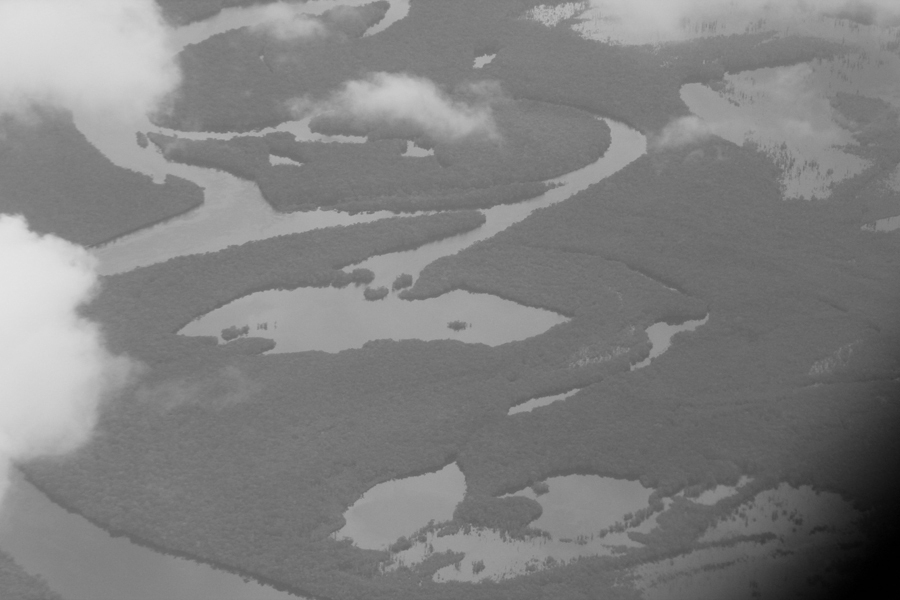
\includegraphics[width=\textwidth]{./img/001}
%\caption{Imagem aérea de afluente do rio Negro (foto: Sylvia C. Novaes, 2012)}
%\end{figure}


A viagem ao Tiquié é adiada a cada dia. A falta de chuvas ou o excesso
de tempestades, o motor quebrado ou a falta de gasolina na cidade, a
doença ou a espera das autorizações de entrada na Terra Indígena fazem
com que o pesquisador fique sempre mais dias no meio urbano do que
imaginava. Em meio a cervejas e caxiris, a pães e beijus, a bifes e
carne de caça, surgem os primeiros laços de amizade. É com indignação
que se começa a ouvir falar da morosidade na demarcação das Terras
Indígenas, da escravidão por dívidas, da violência contra a mulher, da
desatenção à saúde, da falta de estrutura educacional, da corrupção na
prefeitura, do tráfico de drogas. A difícil situação da população local
talvez desperte o desejo de contribuir com o movimento\footnote{A
  Federação das Organizações Indígenas do Alto Rio Negro ({\textsc{foirn}}) é uma
  associação civil fundada em 1987 que se constitui como a principal
  expressão do movimento social e político indígena da região.} e
associações indígenas na busca por melhores condições de vida. No meu
caso, foi também o tempo de acompanhar e assessorar os Hupd'äh em suas
tentativas de obter documentos, benefícios sociais e de participar mais
ativamente do movimento político em busca de melhorias para suas
comunidades.

No porto, a voadeira espera. É chegado o dia da viagem com destino ao
rio Tiquié. Apesar da grande quantidade de roupas, comidas e
equipamentos, resta sempre a sensação de estar se esquecendo de algo.
Acompanhar o dia a dia da pesca, dos trabalhos na roça, das viagens, das
incursões à caça, das festas e das rodas de coca exige a preparação para
inserir"-se em um modo de vida em tudo diferente daquele do morador de
uma grande cidade como São Paulo. Os prédios, as avenidas, as pessoas, a
violência, os barulhos soam aos Hupd'äh como imagens de um meio ao mesmo
tempo estranho, fascinante e perigoso. Nos longos períodos de campo,
minha saudade da família e da esposa comovia sempre meus companheiros.
Queriam integrar"-me a todo custo a seus afazeres, conversar comigo e
nunca me deixar só. Nesse zelo constante, misturavam"-se pena e
solidariedade.

A voadeira vai cortando as águas. O vento forte e o barulho do motor
dificultam as conversas dos tripulantes. Os olhos certamente já estão a
vagar pelo verde das margens. À frente, araras azuis passeiam suavemente
pelo ar. Tucanos pousam nas árvores do lado de lá. Cutucando"-se e
apontando morros, clareiras e aldeias, os companheiros de viagem mostram
lugares, lembram casos e vão ensinando as primeiras lições ao
recém"-chegado. Páginas de livros, imagens de fotografias, cenas de
filmes, palavras de familiares talvez circulem pelos pensamentos do
tripulante. As etnografias lidas falam sobre o povo do barqueiro
Marcelino Massa, um sábio desano que conduz com firmeza o barco.
Denunciam a exploração e violências sofridas pelos parentes barés do
auxiliar de enfermagem Alair Pimenta, que viajou tantas vezes ao meu
lado para atender seus pacientes hup. Descrevem as guerras combatidas
pelos antepassados de Cecília Piratapuia, ex"-freira, liderança
importante para o fortalecimento da participação feminina na Secretaria
das Mulheres da Federação das Organizações Indígenas do Rio Negro
({\textsc{foirn}}), que sentava"-se mais à proa da embarcação durante a viagem que
fizemos juntos.

Grandes morros de pedra emergem da planície amazônica. O vento forte
parece roubar o som das palavras dos viajantes. O pouco que se escuta
vai transformando as formações rochosas em antigas moradas de heróis
criadores do universo. Algumas clareiras ciliares revelam casas de
alvenaria ou madeira com seus telhados indecisos entre a palha do caranã
e as folhas de zinco da Eternit. Nos arranjos comunitários, uma
igrejinha desbotada sempre faz par com uma escola azul e amarela pintada
há pouco. De povoados desconhecidos, as aldeias passam a ser os sítios
onde vivem diversas pessoas de algum modo ligadas aos tripulantes, entre
primos, amigos, um irmão, conhecidos, um tio"-avô ou uma cunhada.

Com o barulho do motor, as crianças que brincam à beira"-rio correm para
perto de suas casas. No porto, as canoas balançam com o banzeiro de
nossa embarcação a aproximar"-se. Na pequena praia, mulheres de longos
cabelos negros arremessam com força as roupas que lavam contra as
pedras. Um sino toca. A aula vai começar. As crianças saem das casas com
seus uniformes de cor amarela e azul que, na região, chamam"-se
``fardas'', como os uniformes dos militares. O barqueiro desliga o
motor. A voadeira vai vagarosamente empurrando as canoas e ocupando seu
lugar no porto. A fome e a vontade de urinar já tornavam impossível a
continuidade. Num instante, todos arregaçam a barra das calças e pulam
no rio para puxar a voadeira. Monte Alegre era frequentemente o ponto de
nossa primeira parada. O capitão da comunidade vinha cumprimentar os
recém"-chegados e o estranho, o antropólogo, de São Paulo.

Em tempos de seca, quando o rio e os igarapés estão baixos, sempre é
possível trocar sabão, arroz, macarrão e/ou sal por peixes moqueados e
beiju. Depois de muitas viagens, os gostos do aracu, da pimenta e do
beiju impregnam na boca a sensação das boas"-vindas. O som das palavras
impenetráveis da língua tukano, falada alegremente pelos viajantes que
reencontram seus conhecidos, passa a ser uma saudação também para
aqueles que aprendem a sentir"-se bem, participando de conversas em
línguas que não compreendem, e a rir de piadas que não podem entender.
Algumas palavras em português permitem seguir a conversa. Por vezes, os
presentes fazem perguntas ao estrangeiro. As novidades da política
local, dos crimes e das festas são comentadas durante o acolhimento e a
partilha da refeição. Pedidos, negociações de trocas e conselhos marcam
a despedida nessas paradas.

A voadeira retoma seu curso. Apenas o barqueiro identifica o caminho a
seguir no espelho d'água. É preciso passar de um lado ao outro para
respeitar o trajeto delimitado pela marinha. Os olhos do barqueiro
perseguem as pedras submersas do rio. Toda atenção é pouca, pois uma
colisão pode emborcar a voadeira e causar uma tragédia. São muitas as
histórias de incidentes envolvendo os barcos mercantes. Numa época de
seca, viajando durante a noite, o barco do comerciante Candinho colidiu
com uma pedra no rio Tiquié. O casco fendeu"-se e a embarcação, com todas
as cargas e bagagens dos tripulantes, afundou. Ninguém morreu, mas foram
muitas as perdas, principalmente das famílias que voltavam de São
Gabriel trazendo roupas, alimentos e instrumentos de trabalho. ``Já vi
muitos barqueiros experientes virarem'', comentou certa vez Marcelino.

Em todas as viagens, em algum momento, nuvens negras começam a
avolumar"-se no céu. A pequena voadeira segue em direção à cortina de
água a ocultar o horizonte. Uma lona azul de {\textsc{pvc}} fornece o abrigo para
que os tripulantes se protejam da força das águas e do vento. Relâmpagos
e trovões iluminam novamente o dia causando temor ao marinheiro de
primeira viagem. O barqueiro veste seu casaco e ajeita seu boné. Segue
firme contra a tempestade. É comum que, depois de horas de precipitação,
o céu volte a se abrir e o sol retome seu brilho. Recolhe"-se a lona,
ajeitam"-se as caixas e os tambores de gasolina da embarcação. Da mata
até o céu, um arco"-íris por vezes contrasta com o cinza das nuvens e com
os diversos tons de verde da mata. Pode ser que uma garça atravesse o
rio bem perto da proa do barco. Branca, desenha no ar um voo rasante.
Pousa sobre uma pedra e acompanha a passagem da voadeira.

Ao longe, avista"-se uma grande igreja. O barqueiro informa que o
distrito de Taracuá se aproxima. O vilarejo é resultado das atividades
dos missionários salesianos. Junto à igreja, uma enfermaria e uma escola
materializam os pilares do projeto civilizatório católico. Velhas
freiras italianas vivem ainda nas casas da missão junto com as freiras
tukano, atualmente em maior número. Certa vez, Cecília contou que nos
anos 1950 o então presidente da república Juscelino Kubitschek pousou de
avião na pista de Taracuá para conhecer de perto as ações missionárias
que, de acordo com o Estado, visavam à integração dos indígenas à
sociedade nacional. Nosso barco parou muitas vezes no porto do vilarejo,
em meio às canoas e a outras voadeiras de alumínio. Precisa"-se descer e
procurar um lugar para dormir, pois o fim da tarde se aproxima e não é
prudente a viagem noturna. Pede"-se ao capitão local a permissão para o
repouso no barracão comunitário. É lá onde dormem os viajantes que
participam dos cursos, reuniões e festas promovidas pelo movimento
indígena. Com um fogareiro preparam"-se os enlatados que se somam ao
peixe moqueado, à pimenta e ao beiju. Redes atadas, todos apagam as
lanternas e deitam"-se com os corpos consumidos pela viagem.

Na penumbra, o sol mal começa a tatear o breu do horizonte e os
viajantes já estão retornando de seus banhos de rio. A refeição matinal
é rápida, pois talvez haja a possibilidade de chegada, no final da
tarde, à comunidade de Taracuá"-Igarapé, nosso destino final. A voadeira
deixa o porto em meio ao vento frio que faz tremer o corpo e ansiar pelo
calor do dia. Depois de uma curva acentuada, o barco despede"-se do rio
Uaupés e penetra as águas do rio Tiquié. As margens estreitam"-se e o
curso d'água revela o tecido rochoso de seu leito. A monotonia do
percurso retilíneo do rio Negro e do Uaupés dá lugar a um itinerário
sinuoso e repleto de paranás. Mais próxima, a vegetação começa a
oferecer"-se menos homogênea em seus tons de verde e de marrom. Flores,
folhas, troncos, arbustos tomam infinitas formas. As trepadeiras,
paxiúbas, paus"-brasil, samambaias, pupunheiras, seringueiras talvez
estejam entre as poucas espécies reconhecidas pelo principiante. No alto
das copas, macacos"-prego, macacos"-barrigudos e provavelmente uma
preguiça se mostram ao viajante.

Nas idas ao Tiquié, talvez uma falha no motor possa reduzir sua
potência. A velocidade passa a ser inferior à metade da empregada em
condições normais, apesar dos esforços do barqueiro em acelerar. O
carburador pode estar sujo. Com sorte, chega"-se à comunidade de Serra do
Mucura antes do pôr do sol para limpar o carburador e descansar. Com a
diminuição da velocidade, acompanha"-se, por alguns instantes, a viagem
das canoas movidas a rabeta. Elas levam os moradores das comunidades do
Tiquié aos vilarejos de Taracuá, Pari"-Cachoeira, outra antiga missão
salesiana, e mesmo a São Gabriel da Cachoeira. Repletas de gente e, em
alguns casos, de caixas com mercadorias, as pequenas embarcações parecem
quase virar a cada ondulação do banzeiro. Com a passagem do barco, todos
que estão na canoa levantam os braços e acenam. Para proteger"-se do sol,
as mães abrigam seus filhos em um guarda"-chuva. As crianças animam"-se
com a passagem da voadeira e sorriem.

Com muito custo, depois de oito horas de viagem, chega"-se à comunidade
de Serra do Mucura. Muitos barqueiros têm fortes laços de amizade com os
moradores dessa aldeia. Alguns dos moradores são considerados ótimos
artesãos e participam do projeto de uma {\textsc{ong}} que criou uma rede de
distribuição e venda de bancos tradicionais nos grandes centros urbanos
do país. O capitão sempre vem ao nosso encontro e nos recebe
calorosamente. Geralmente nos instalamos na casa comunitária onde, sobre
uma mesa, beijus, peixes moqueados e uma quinhampira, caldo de peixe e
pimenta são colocados como oferecimento aos viajantes. Partilhamos a
comida e depois bebemos o chibé, uma refrescante água com farinha. Em
minhas últimas viagens, as eleições municipais e a compra de votos por
parte de alguns candidatos foram temas correntes das conversas e das
piadas. Um dos candidatos, dono de postos de gasolina, distribuíra
combustível de graça para alguns eleitores. Como havia adicionado água à
gasolina, muitas pessoas que voltavam da cidade em suas rabetas ficaram
ilhadas e tiveram que pedir carona para conseguir chegar a suas casas.

À noite, depois do banho, o capitão me fala da vontade que todos têm de
me ouvir tocar violão. Eu começo, então, a dedilhar algumas modas
caipiras. Para minha surpresa, nas minhas primeiras visitas, ouvi os
outros cantarolarem suavemente comigo alguns versos das canções.
``Menino da porteira'' e ``Chico Mineiro'' são sempre as mais pedidas.
Antigamente, as rádios regionais tocavam muito as modas de viola e
familiarizavam os ouvintes com esse estilo musical. Isso permite que meu
repertório seja apreciado com gosto. Por volta das 20h30, nossos
anfitriões, satisfeitos com a cantoria, despedem"-se e, muito cansados,
retiram"-se para suas casas. Nós atamos nossas redes e rapidamente caímos
no sono.

Logo cedo, a mesa já está repleta novamente de mingau, moqueados e
beijus. Conversamos sobre minha pesquisa e sobre o tempo que eu teria de
permanecer na comunidade de Taracuá"-Igarapé. Como minhas primeiras
incursões à região se deram através do trabalho com saúde pela
Associação Saúde Sem Limites (\textsc{ssl}), em toda conversa falamos muito sobre
os atendimentos das equipes de saúde do \textsc{dsei}"-\textsc{rn}. As reclamações sobre as
poucas visitas de atendimento, os remédios vencidos, a demora nos
resgates, a falta de cursos para os Agentes Indígenas de Saúde (\textsc{ais}) e a
falta de médicos dão o tom das falas indignadas. Meu caderno de campo
inicia"-se com notas sobre essas queixas que depois compõem meus
relatórios técnicos em denúncia de tal situação à \textsc{foirn} e ao Controle
Social\footnote{O Controle Social é uma estrutura composta por conselhos
  nacionais, estaduais e municipais dos quais participam representantes
  comunitários e lideranças de movimentos sociais para fiscalizar a
  condução das políticas públicas em saúde.}.

De volta ao barco, nos preparamos para enfrentar o percurso do
Igarapé"-Taracuá, o /Ta̗t"-Dëh/. Passadas algumas horas de navegação pelo
rio Tiquié, chegamos à comunidade de Cunuri, aldeia tukano onde
atualmente vivem também famílias desano e tuyuka. Um caminho pela mata
leva os cerca de duas horas à aldeia hup. É para lá que algumas famílias
do Cunuri vão para realizar trocas com os Hupd'äh, demandar auxílio no
trabalho das roças, solicitar que benzedores hup executem encantamentos,
ou para fazer visitas e participar das festas de caxiri de /Ta̗t"-Dëh/.
Contam os Tukano que o antigo dono da comunidade foi quem autorizou os
Hupd'äh a constituírem sua aldeia nesse território que consideram seu.
Com a parada no Cunuri, conhecem pessoas tukano que participam da
sociabilidade da aldeia hup. Ouvem também conselhos sobre a melhor forma
de navegar pelo Igarapé"-Taracuá.

O barco mal entra no Igarapé"-Taracuá e já é possível perceber as
dificuldades que serão enfrentadas no percurso. O caminho d'água
torna"-se estreito e raso. Muitas vezes é preciso que todos desçam do
bote para empurrá"-lo. Em momentos mais difíceis, deve"-se retirar as
caixas de mantimentos e equipamentos para diminuir ainda mais o peso da
embarcação e empurrá"-la com força, para que ela aos poucos vá deslizando
pela areia e encontre área de maior profundidade. Árvores caídas fazem
com que os viajantes desçam com seus terçados para ``torar'' o tronco
até cindi"-lo ao meio. Toda a atenção é pouca, pois grandes aranhas e
cobras costumam surgir em meio aos troncos e galhos. Vez ou outra, o
barulho do grupo que se aproxima assusta um veado. ``Se tivesse uma
espingarda à mão'', lamentam"-se todos.

Passadas longas horas nesse trabalho que exige grande esforço, surge
finalmente o porto de areia da comunidade de /Ta̗t"-Dëh/. Tendo ouvido já
há horas o barulho do motor de popa, muitas pessoas correm para a beira
para ver e saudar quem está chegando. Depois de algumas viagens, foi com
imensa saudade que passei a acenar aos moradores de /Ta̗t"-Dëh/, que foram
se tornando grandes amigos. Do estranhamento das primeiras estadas,
comecei também a perceber os sorrisos e cumprimentos afetuosos depois de
meses de distância.

Passei a entender também que meus interlocutores são, antes de mais
nada, viajantes sedentos pelas notícias das terras distantes. O
desbravamento das muitas ``coisas dos brancos'' como carros, cachaças,
casas, comidas, roupas, músicas, filmes vem ocorrendo através das
constantes viagens a São Gabriel. Essas idas ao centro urbano
alternam"-se com as andanças pela mata para a pesca, caça e visita a
parentes, que são também uma fonte inesgotável de causos e lembranças.
Mas suponho que o gosto pelas notícias que eu trazia e o interesse por
São Paulo tenham algo a ver com a própria história de origem de seus
ancestrais, os /hib'ah te͂h d'äh/. Saídos do Rio de Janeiro, do
/Pu̗d"-dëh"-moh/, o ``Lago de Leite'', os antepassados dos Hupd'äh viajaram
por muito tempo dentro da /M'e̖h Hõh Tëg/, a ``Cobra"-Canoa''. Depois de
ter chamado os seres humanos à existência, /K'e̖g Te͂h/ fez a Cobra"-Canoa
e mandou que todas as Gentes"-Peixe embarcassem e rumassem para a região
do Uaupés. Alguns não aguentaram a viagem longa e penosa, caíram da
Cobra"-Canoa e vivem hoje nas /Dëh"-Mo̖y/, ``Casas"-do"-Rio'', que existem
nas profundezas dos rios Negro, Uaupés e Tiquié. Esses continuaram a ser
Gente"-Peixe, não se transformaram em Hupd'äh e, por isso, causam doenças
e vivem tentando roubar nossos ``espíritos''.

A Cobra"-Canoa foi abrindo o caminho dos rios pelos quais viajamos hoje
em dia. Foi na cachoeira de Ipanoré, /Hib'a̖h Hu͂h/, que os ancestrais dos
diversos clãs hup emergiram pelos buracos que há nas rochas. Depois da
longa viagem, foi lá que os primeiros hup sentaram para conversar
enquanto comiam a coca, fumavam tabaco e bebiam caarpi. Talvez o
fascínio com que os Hupd'äh contam sobre a viagem de seus antepassados
na Cobra"-Canoa tenha algo desse encantamento com um mundo completamente
diferente daquele que eu vinha experienciando ao longo de minha vida.
Foi com esse encantamento também que comecei a viajar pelos rios da
região do Alto Rio Negro, a sentar"-me nas rodas de coca, a ouvir sobre
as viagens dos antigos, e a andar pelos caminhos das matas.

%\begin{figure}
%\centering
 % 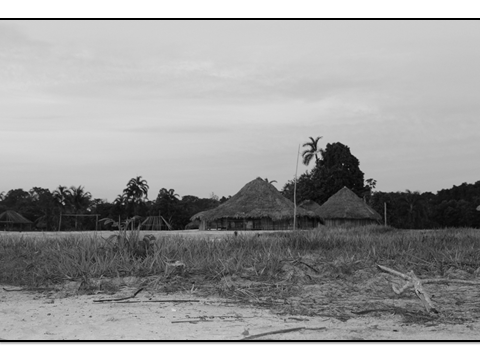
\includegraphics[width=\textwidth]{./img/002}
%\caption{Vista da aldeia de /Ta̗t"-dëh/ (Foto: Sylvia C. Novaes, 2012)}
%\end{figure}

\section{Encontros noturnos e caminhos
vividos}\label{encontros-noturnos-e-caminhos-vividos}

O velho Henrique está morto. A notícia chegou naquela tarde por
\emph{e"-mail}. A fumaça do cigarro deixava minha boca e tateava
lentamente o ar frio. O traumatismo craniano ocasionado por uma queda no
banheiro mal equipado do posto de saúde fez com que ele morresse dias
depois do acidente. Como aprendi, seu espírito viajava naquele momento
para a /Paç Pö̗g/, a ``Serra Grande'', onde coabitaria com seus
antepassados. Mais tarde, ascendendo, o percurso o levaria à casa do
criador, /K'e̖g Te͂h/. ``No próximo ano não estarei mais aqui'', ele me
disse em língua hup no momento em que o abracei, despedi"-me, e dei a ele
minha rede. O calor da febre e as tosses causadas por uma forte gripe
não o deixavam descansar. Uns dias antes, ele acordou triste e contou ao
filho um sonho. Tinha sido levado para o fundo da Terra pelos /K'öd
d'äh/. Disse a eles que não era de lá. Mandaram que seguisse um
beija"-flor/canoa para chegar novamente à Terra. Acordou triste. O sonho
mostrava que seu ``espírito'', /ha̗͂wäg/, estava deixando seu corpo. Eu
não poderia mais acender seus cigarros, ouvir suas histórias nas rodas
de coca nem cantar com ele os caapivaiás.

O velho Henrique (/B'o̖'/, falecido, /Sokw'ä̗t Noh K'öd Tẽ̖h/) foi
a primeira pessoa hup que conheci logo que cheguei à cidade de São
Gabriel da Cachoeira, em 2007. Ficamos juntos alojados na casa da
Associação Saúde Sem Limites (\textsc{ssl}), onde ele recebia cuidados médicos e
eu aguardava a viagem com a equipe da \textsc{ong} para realizar um diagnóstico
participativo em comunidades hup quanto aos impactos da suposta
sedentarização sobre a saúde e a qualidade de vida dessa população.
Almoçávamos e jantávamos juntos e, de alguma forma, nos comunicávamos,
cantávamos e fazíamos companhia um ao outro. Quando comecei meu trabalho
de campo em 2009 na aldeia de Taracuá"-Igarapé, /Ta̗t"-Dëh/, tomávamos café
pela manhã, comíamos juntos no início da tarde, cantávamos e gravávamos
os cantos do caapivaiá e, no início da noite, íamos participar dos
encontros noturnos para comer coca, fumar, ouvir histórias e
benzimentos. Acredito que esse laço que nos unia esteja relacionado com
o modo como foram se estabelecendo os contornos da etnografia sobre as
rodas de coca e os caminhos vividos pelos Hupd'äh.

Ao pôr do sol, quando o som do pilão começa a soar na aldeia, é possível
acompanhar os passos dos senhores hup que vão caminhando vagarosamente e
se reunindo atrás de uma casa na periferia da comunidade. Alguns
encontram banquinhos. Outros repousam seus corpos sentando no chão de
areia. Aos poucos, é possível ver uma roda surgir em torno do pilão que
vai triturando a coca e as folhas queimadas de imbaúba. Enquanto isso, a
fumaça cinza vai se espalhando pelo ar e cigarros movimentam"-se nas
bocas. As saudações são acompanhadas de risos e piadas, e seguidas por
comentários sobre as andanças pelos caminhos para a pesca, caça ou
colheita de folhas de coca. A mistura de coca e imbaúba é então
derramada numa cuia que começa a circular de mão em mão. Lembro"-me de
que o velho Henrique era sempre o primeiro a receber a coca por ser o
mais velho da comunidade. Cada participante vai derramando a coca na
boca à medida que histórias são contadas e encantamentos ensinados.
Murmurando palavras para cigarros ou cuias, alguns dos presentes começam
também a executar ações xamânicas para curar ou proteger pessoas.

A pesquisa de campo foi realizada principalmente na comunidade hup de
Taracuá"-Igarapé, /Ta̗t"-Dëh/, na qual habitam aproximadamente 202
indivíduos e que está situada em território hup às margens do igarapé de
mesmo nome, afluente do rio Tiquié. Há, ao todo, vinte e seis casas onde
moram 38 grupos domésticos. O clã /Sokw'ä̗t Noh K'öd Tẽ̖h/ é majoritário e
reivindica a posse do território, das áreas de caça, pesca e roça. Há
também a presença de muitas famílias que, na geração atual, se
identificam como pertencentes ao clã /Dög M'e̖h Tẽ̖h D'äh/, grupo afim aos
/Sokw'ä̗t Noh K'öd Tẽ̖h D'äh/. Essas famílias dizem ter pertencido
anteriormente à etnia Dâw, mas por diversas razões estão se tornando
Hupd'äh, esquecendo sua língua e benzimentos, casando"-se com pessoas hup
e assumindo a identidade desse clã. Em algumas noites, mais de uma roda
para o consumo de coca pode se formar. A principal delas ocorre
diariamente e conta com a participação de aproximadamente 10 pessoas,
tendo como referência o senhor Ponciano (/Hu̖d/, 05/07/1946, Sokw'ä̗t Noh
K'öd Tẽ̖h). Uma outra, da qual participam em média 6 pessoas, se
forma próximo à casa do pajé Firmino (/B'o̖'/, 06/07/1947, /Sokw'ä̗t Noh
K'öd Tẽ̖h/). Em /Ta̗t"-Dëh/, além de Firmino, Armando (/Kä'/,
05/01/1948, /Sokw'ä̗t Noh K'öd Tẽ̖h/) também é identificado como
/sä̗w/, ``pajé'', e realiza curas xamânicas. Entretanto, todos os
participantes das rodas praticam o xamanismo, sendo vistos
principalmente como /bi'i̖d d'äh/, ``benzedores''. Dessa forma, tanto
pela intensidade com que se realizam as rodas quanto pela existência dos
pajés e benzedores, essa comunidade mostrou"-se como de especial
relevância para a pesquisa.

Foi sentando"-me às rodas de coca que comecei a ser convidado para seguir
meus interlocutores pelos caminhos que atravessam a floresta. Os
chamados /hup ti̖w/, ``caminhos de hup'', iniciam"-se como continuações
dos trajetos para as roças que vão se estreitando aos poucos até
formarem trilhas fechadas que se diferenciam sutilmente da densa mata.
Seguindo por esses percursos, as pessoas se dirigem diariamente aos
igarapés para a pesca, deslocam"-se para outras aldeias, seguem os
rastros de animais ou realizam viagens para os morros situados nas
cabeceiras. Em meio a seus movimentos, os andarilhos passam pelas
/Moy"-Höd/, ``Moradas Antigas'', onde seus antepassados habitaram antes
de viver na grande aldeia de /Ta̗t"-Dëh/. Chegam a lugares impregnados
pela ação de demiurgos cujos feitos são narrados até hoje nas /pɨnɨ̖g/,
``mitos/histórias''. Descobrem, assim, sentidos imanentes ao mundo que
vão se revelando à medida que os viajantes se situam nessas outras
paisagens e aceitam interagir com animais, plantas, ancestrais e demais
seres com quem coabitam.

Sentados nos encontros noturnos, os senhores hup revelam"-se viajantes a
narrar seus percursos pelo mundo através dos ``caminhos'', /hup ti̖w/, e
dos deslocamentos xamânicos. O trabalho de campo realizado entre 2009 e
2012 permitiu perceber que as rodas de coca constituem"-se como uma forma
constante de interação central para os fazeres mítico e xamânico, a
partir dos quais os senhores estabelecem relações fundamentais com o
universo hup. Seus movimentos fazem"-nos passar por lugares onde eventos
míticos ocorreram, visitar paisagens habitadas por seres diversos e
praticar ações rituais no alto de morros como a Serra Grande.

Compartilhar as cuias de coca com o senhor Henrique, ouvir seu sonho de
deslocamento para a morada subterrânea dos /K'ö̗d däh/, testemunhar sua
morte pelo descaso em São Gabriel, e saber de seu percurso póstumo à
Serra Grande motivaram"-me a ocupar um lugar nas rodas e a aceitar seguir
meus mentores em viagens por seus caminhos vividos. Ao longo da
pesquisa, entendi que os encontros noturnos podem ser vistos como um
\emph{modo de ação} que permite aos participantes constituírem
\emph{percursos de observação} a partir de seus próprios movimentos em
meio às palavras sopradas dos encantamentos e aos passos trilhados pelos
caminhos que atravessam a floresta. As rodas de coca, tão importantes
para o senhor Henrique, passaram a ser vistas por mim como
\emph{performances} onde, em meio à sequência dos encontros e viagens,
ocorrem múltiplas \emph{condensações rituais}, tornando determinados
gestos, posturas, palavras e substâncias fundamentais para a interação
com todos aqueles com quem os Hupd'äh partilham paisagens e saberes.
Espero, com esse trabalho, descrever um pouco esses aspectos da
existência dos Hupd'äh que, com a amizade de Henrique, começaram a fazer
parte de minha própria história.

\section{Olhares para os Hupd'äh}\label{olhares-para-os-hupduxe4h}

Os Hupd'äh habitam a região do Alto Rio Negro (\textsc{am}), na fronteira entre o
Brasil e a Colômbia. Suas comunidades situam"-se às margens de igarapés
da área interfluvial dos rios Tiquié e Papuri, afluentes da margem
esquerda do rio Uaupés. Os dados demográficos mais atuais, de acordo com
a pesquisa de Epps (2005) e Athias (2006) estimam a população num total
de 1.500 indivíduos distribuídos em aproximadamente 35 aldeias. A alta
mobilidade e circulação pelo território são aspectos fundamentais do
modo de vida hup, que estão relacionados ao vasto conhecimento que
possuem sobre os caminhos, os igarapés, os animais e a vegetação local.
Associada à mobilidade, a caça"-coleta constitui"-se como foco de
interesse das pesquisas antropológicas sobre esse povo, estabelecendo o
contraste entre os Hupd'äh com as populações ribeirinhas de
pescadores"-agricultores. Ao mesmo tempo, a constância da caça"-coleta tem
diminuído nas últimas décadas, fazendo com que a pesca em igarapés e as
roças de mandioca venham se tornando cada vez mais fundamentais para a
produção alimentar, principalmente nas comunidades mais populosas.
Atualmente, há algumas aldeias que agregam de 100 a 200 indivíduos,
enquanto outras continuam concentrando de 15 a 50 pessoas, como parece
ser o padrão descrito pelos pesquisadores. Conforme mostra Athias, em
sua pesquisa de 1995, o aumento populacional e a maior duração da
permanência da morada num local próximo aos grandes rios têm a ver com a
agência missionária salesiana, que procurou agregar em grandes aldeias,
designadas pelo pesquisador como povoados"-missão, o maior número de
pessoas para evangelização.

\begin{figure}
\centering
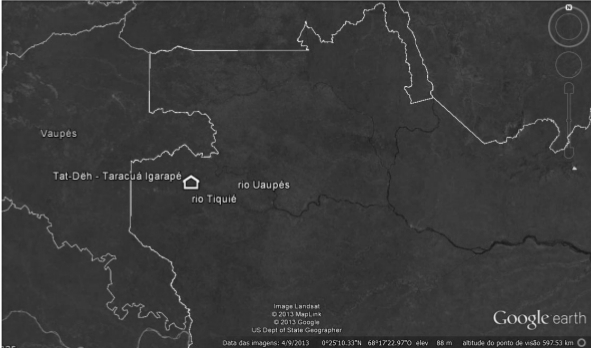
\includegraphics[width=\textwidth]{./img/003}
\caption{Localização da comunidade Hupd'äh de /Ta̗t"-Dëh/,
Taracuá"-Igarapé}
\end{figure}

A estrutura social hup tem nos clãs agnáticos seus segmentos básicos de
constituição e de diferenciação. Criados pelo herói cultural /K'e̖g Te͂h/,
os ``ancestrais'', /hib'a̗h"-tẽ̖h"-d'äh/, deram origem aos hoje
aproximadamente 25 clãs exogâmicos e de descendência patrilinear. Cada
clã possui um conjunto específico de nomes, mitos e cantos por meio dos
quais são narrados os eventos de criação e se constitui um senso de
pertencimento e identidade. O casamento preferencial dá"-se entre os
primos cruzados bilaterais numa mesma geração e procura respeitar certa
hierarquia entre os clãs. Em contraste com outros povos da região, o
sistema de matrimônio dá"-se segundo a endogamia linguística e a exogamia
clânica. O casamento dá origem a grupos de fogo, unidades mínimas de
produção e consumo. A coabitação em um mesmo território ou espaço de
grupos de fogo gera os grupos locais, que são nomeados e diferenciados
entre si. Os deslocamentos de grupos de fogo ou indivíduos para visitas
a parentes de outros grupos locais ocorrem periodicamente e podem durar
meses.

Esses traços aproximam os Hupd'äh de povos como os Yuhupdëh, Nadëb, Dâw,
Kákwa e Nukák, permitindo que fossem designados pela literatura
etnológica da região como povos maku. Entendendo haver um sistema
relativamente homogêneo baseado na exogamia linguística, nas relações
hierárquicas rituais e territoriais entre povos falantes de línguas
tukano e arawak, os pesquisadores descrevem a especificidade da
articulação dos povos maku a esse ``sistema vaupesiano''. O próprio
termo ``maku'', adotado pela literatura, revela a particularidade dessa
interação, já que a palavra maku origina"-se do arawak e significa
``aquele que não tem fala'' ou ``aquele que não tem a nossa fala'' (ma =
prefixo privativo/aku = fala), sendo associado a ``selvagem'', a
índios"-da"-floresta em oposição a índios"-do"-rio, como os povos tukano e
arawak. A realização de trabalhos nas roças de famílias tukano, que faz
com que famílias maku se mudem para um local próximo às aldeias tukano
em determinados períodos, as trocas de carne de caça e frutos por
mandioca, peixes e mercadorias, e o respeito e silêncio diante dos
tukano são aspectos que fizeram com que os pesquisadores descrevessem as
relações entre esses povos como simbióticas, de patrão/cliente,
hierárquicas/assimétricas.

Segundo a linguista Patience Epps (2005), os traços semelhantes entre as
línguas hup, nadëb (kuyawi), dâw e yuhup constituem"-nas como línguas
irmãs, formando assim uma família linguística. Ela propõe que essa seria
a família nadahup ou, como vem sendo designada por outros estudos, a
família maku. Há também pesquisadores que incluem as línguas kákwa
(bara"-maku) e nukák como pertencentes a essa família. O trabalho de
Epps, \emph{A Grammar of Hup}, de 2005, coloca"-se como o primeiro estudo
mais aprofundado da língua hup. Até hoje, a língua hup é a primeira a
ser falada pelas crianças hup. Dado seu relativo isolamento, poucos
falantes de hup são fluentes em português. Apesar disso, virtualmente
todos são falantes da língua tukano, uma língua tukano oriental falada
pelas etnias próximas que serve como uma língua franca regional. A
partir de 2001, ações da secretaria da educação local e de \textsc{ong}s
implantaram um sistema de formação de professores hup, dâw e yuhup, com
o objetivo de consolidar as escolas desses povos. Começa, a partir de
então, um processo de descrição da língua hup, fixação da grafia,
compreensão dos princípios gramaticais, e alfabetização inicial dos
professores. Foram elaborados um dicionário hupd'äh"-português e
cartilhas na língua hup. Esses materiais vêm permitindo aos professores
desenvolver junto aos alunos a escrita e o aprendizado de sua língua.

\begin{figure}
\centering
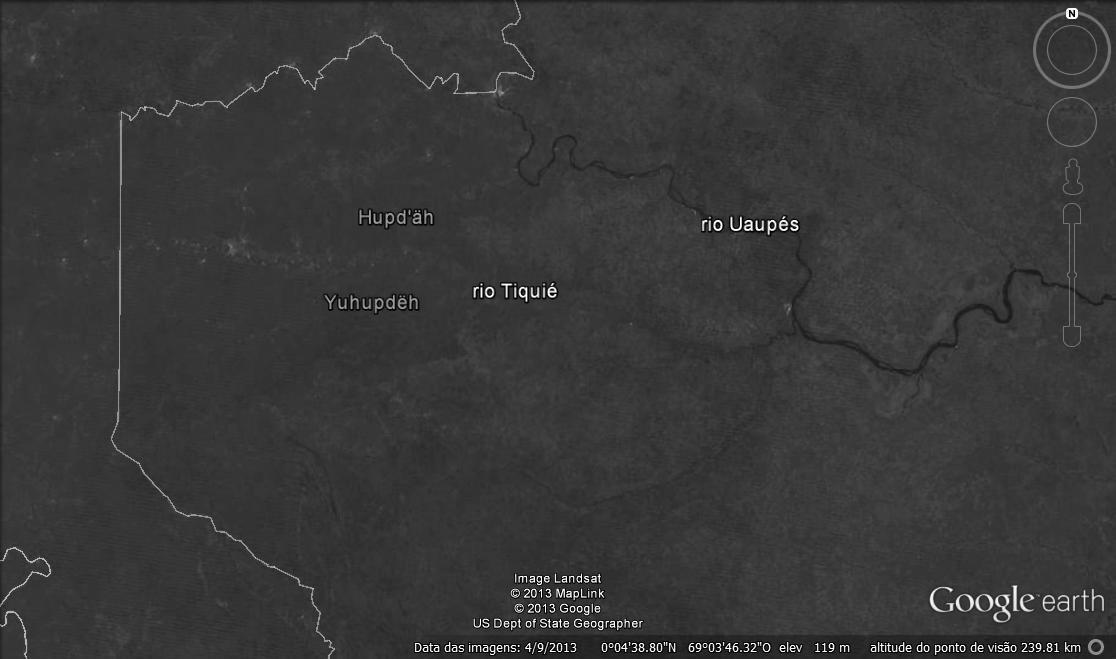
\includegraphics[width=\textwidth]{./img/004}
\caption{Regiões habitadas por populações das etnias hupd'äh
e yuhupdëh no médio Tiquié}
\end{figure}

O contato teve inicio com as frentes de colonização desde o século
\textsc{xviii}, mas foi apenas nas décadas de 1960 e 1970 do século \textsc{xx} que os
missionários salesianos iniciaram atividades mais intensas visando à
evangelização e à escolarização dos Hupd'äh. Trabalhando já há décadas
com os Tukano, os padres salesianos pretendiam intervir nas relações
vistas como assimétricas entre esses povos. A constituição de aldeias
hup em território tukano e o aumento populacional das comunidades podem
ser vistos como processos influenciados pela ação missionária.
Paralelamente, observa"-se a dificuldade crescente na obtenção de
alimentos, o aumento na taxa de mortalidade e de doenças, e o constante
recrutamento e exploração de mão de obra para atividades extrativistas
(borracha e cipó). Nos últimos anos, as atividades das equipes de saúde,
de indigenistas, e de missionários pentecostais vêm somando"-se à ação
dos salesianos que ainda mantêm suas ações em uma aldeia hup e na região
do Alto Rio Negro como um todo.

\asterisc{}  

Certa vez, enquanto eu lia a tese de Howard Reid em meu computador,
Ricardo se lembrou das histórias do antropólogo que usava tanga, falava
hup, caçava e pescava.

\begin{quote}
Mostrei a Ricardo o livro de Howard Reid. Ele disse que os velhos
falaram pra ele desse que chamavam Haw. Ele usava tanga. Ficava lá no
meio deles. Falava a língua hup. Ia caçar no mato, pescava, fazia tudo
como os Hupd'äh. Ele e o Peter (Peter Silverwood"-Cope). Ele falava pros
velhos que veio de avião. Eles gostavam desse /Haw/. Mas ele foi embora
e não voltou mais. O avô de Ricardo conheceu"-o. Ele foi embora uns anos
antes de Ricardo nascer (Caderno de campo, 25/11/2009).
\end{quote}

Durante minhas estadas em campo, sempre ouço também histórias dos
pesquisadores que me precederam. De formas diferentes, a imagem desses
``brancos'' que ``viviam com e como os índios'' sobrepõe"-se à minha.
Distante das comunidades, encontro"-me com o /Haw/ quase sempre. Seus
trabalhos guiam"-me por muitos percursos florestais que permeiam minhas
experiências partilhadas com os Hupd'äh. Como tenho ouvido em muitas
conversas, a relação com os senhores hup parece ter sido marcante também
para Reid.

Há poucos trabalhos antropológicos sobre os grupos maku. Dentre os
existentes, destacam"-se os de Peter Silverwood"-Cope (1972/1990) sobre os
Bara"-Maku (Kakwá), de Howard Reid (1979) sobre os Hup'däh, de Renato
Athias (1995) sobre os Hup'däh e Tukano, de Jorge Pozzobon (1983, 1991)
sobre diversos povos maku e, mais recentemente, o trabalho de Pedro
Lolli (2010) sobre os Yuhupdëh. Desses, apenas o trabalho de Reid
apresenta uma monografia extensa sobre os Hupd'äh. Athias enfatiza a
relação interétnica entre os Hupd'äh e os Tukano. Pozzobon (1991), por
sua vez, enfoca os sistemas de parentesco e as regras de casamento dos
Yuhupdëh, Hup'däh, Dâw, Kákwa e Nadëb. Tomando como referência a leitura
crítica da literatura sobre os povos maku feita por Bruno Marques
(2009), passo agora a uma breve discussão a respeito dos trabalhos dos
pesquisadores que se dedicaram ao estudo dos povos maku.

O primeiro estudo etnográfico detalhado sobre um grupo maku, os
Bara"-Maku (Kákwa), foi realizado por Peter Silverwood"-Cope em 1972. O
autor salienta que um dos objetivos de sua pesquisa foi o de contribuir
para aumentar o conhecimento sobre os povos maku, já que era reduzido o
número de pesquisas e eram poucos os dados existentes até então. Antes
de seu estudo, autores como Giacone (1969), Koch"-Grünberg (1906/2010),
Biocca (1965) e Münzel (1969) apresentaram apenas listas de palavras,
descrições gerais da cultura material, comportamento e rituais,
transcrições de mitos e resenhas bibliográficas.

Em outubro de 1968, Peter Silverwood"-Cope viajava com Stephen e
Christine Hugh"-Jones para o rio Pira Paraná em busca de grupos maku na
região. O fato de não ter encontrado tais grupos nessa área fez com que
o antropólogo consolidasse sua pesquisa com um único grupo regional
bara"-maku (kákwa), da região do rio Macu"-Paraná. Sua pesquisa apresenta
uma descrição detalhada do modo de vida dos Bara"-Maku e, genericamente,
dos Maku, abrangendo as atividades de caça, pesca, coleta e colheita, os
conhecimentos sobre o ecossistema, técnicas produtivas, sistema de clãs,
regras de casamento e categorias de parentesco. Para descrever a
adaptação ecológica dos Bara"-Maku e mostrar a importância da caça para
esse povo, Silverwood"-Cope observa ser fundamental entender a relação
que os grupos têm em diferentes momentos com a aldeia, o acampamento de
caça e a permanência junto aos Tukano para a realização de trabalhos.

Os padrões de caça são descritos através das técnicas utilizadas, de
dados quantitativos sobre produção e consumo, de formas de classificação
e concepções cosmológicas sobre a atividade. Na monografia, é também
estabelecido o contraste entre a adaptação ecológica tukano e maku, e
são descritas as relações de trocas sociais e econômicas entre ambos. A
complexidade revelada por seu trabalho aponta a necessidade da revisão
da categorização desses povos como sendo caçadores e coletores nômades
muito primitivos que, segundo a literatura científica, vinham sendo
assimilados e escravizados por povos agricultores invasores.

Numa perspectiva semelhante, o trabalho de Reid (1979) busca entender a
cultura e o semi"-nomadismo hup através da mobilidade e da fluidez desse
povo em diferentes espaços da floresta; do seu sistema de classificação
e de relações sociais que marcam as distintas fases da vida, e da sua
cosmologia. As mudanças suscitadas pelas atividades dos missionários
salesianos, pelos comerciantes de produtos extrativistas e pela Fundação
Nacional do Índio (\textsc{funai}) são tematizadas na parte final de seu estudo,
realizado num momento de intensificação do contato.

As atividades econômicas e a organização social são apresentadas sempre
em conexão com os conceitos de mobilidade e fluidez. Além do estudo
sobre economia e organização social, Reid realiza também uma
interessante descrição acerca das fases da vida dos Hup'däh, buscando
sempre relacioná"-las aos espaços sociais e às atividades desempenhadas
por cada um em determinados períodos da vida. Para o autor, as mudanças
nos papéis sociais e nas fases da vida contribuem para aumentar, no caso
dos mais jovens, e diminuir, no caso dos mais velhos, a mobilidade entre
os grupos sociais hup. Seu trabalho ressalta também a convergência entre
a classificação dos mitos e do cosmos e o sistema de classificação hup
mais geral.

Para Jorge Pozzobon (1983), a principal contribuição das análises de
Reid e Silverwood"-Cope, quanto aos sistemas de parentesco e de
organização social, foi a de revelar que ``o traço mais marcante da
cultura dos povos maku é a grande fluidez com que eles seguem as
próprias regras de aliança e filiação, sua terminologia de parentesco e
suas regras residenciais''. A partir disso, o objetivo de seu trabalho é
enfocar como esse caráter de fluidez dos Maku está ligado a fatores
demográficos.

O autor percebe haver uma tendência geral para que os Maku procurem seus
cônjuges em círculos endogâmicos cada vez mais restritos, estando esse
princípio relacionado à proporção entre os sexos em determinadas
unidades demográficas. Para Pozzobon, a mobilidade desses grupos liga"-se
mais a fatores sociais e políticos do que a fatores econômicos (caça e
coleta). Os grupos locais funcionam como isolados matrimoniais,
caracterizados pela endogamia e ``um sentimento restrito de
identidade''. Assim, o pesquisador parte da diferença entre a suposta
exogamia prescrita pelas regras de matrimônio e a prática cada vez mais
endogâmica evidenciada por seu recenseamento, e analisa o comportamento
fluido desses povos\footnote{Desse modo, para perceber as dimensões
  relevantes dos sistemas de parentesco e melhor compreender as rodas de
  coca, foi preciso estar atento à diferença entre as regras de
  casamento e à forma como o parentesco se realiza na prática, tendo em
  vista o novo contexto demográfico atual.}.

O estudo de Renato Athias, de 1995, analisa as relações interétnicas
entre os Hupd'äh e os Tukano, e as formas de adaptação de cada etnia ao
ecossistema. Contribui para uma melhor compreensão da organização social
e das relações entre esses povos. Segundo ele, a diferença marcante do
sistema de parentesco e das atividades produtivas faz com que as
relações interétnicas se caracterizem pela assimetria e formem um
sistema hierarquizado. Para o pesquisador, o fato de partir da
perspectiva hup para entender essas relações de subordinação e submissão
com os Tukano faz com que seu trabalho se diferencie das pesquisas
anteriores, que partiam sempre do ponto de vista tukano. Recentemente, o
trabalho de Lirian Monteiro (2011) abordou o tema da relação entre os
Hupd'äh e os Tukano a partir da história da comunidade tukano de
Barreira Alta que, após a migração das famílias tukano para São Gabriel,
passou a ser habitada quase que exclusivamente por famílias hupd'äh.

Como pode se perceber nas pesquisas já realizadas, as narrativas e ritos
são apenas elementos descritos para a composição de um quadro geral
desses povos, surgindo, geralmente, em capítulos destinados à cosmologia
ou em meio à descrição da organização social desses povos. Assim,
tomando como referência os encontros noturnos enquanto forma de
interação social específica, articulada aos movimentos das viagens, o
trabalho que desenvolvi procura delinear o modo como narrativas e
andanças geram importantes condensações rituais que entrelaçam rodas,
caminhos e paisagens como campos de percepção e ação vividos mutuamente
pelas pessoas hup.

\section{Movimentos de emaranhar}\label{movimentos-de-emaranhar}

Sonhar com uma antropologia livre da desumanização dos sujeitos,
transformados pelos estudos em portadores impessoais de ``cultura'',
determinados pelas forças, variáveis e pressões sociais foi o que levou
Victor Turner a buscar os estudos da \emph{performance}. Entendendo que
apenas por meio dessa liberdade seja possível escrever sobre os
encontros noturnos revelando os modos de percepção e as sensibilidades
que são por eles mobilizados, descrevo as rodas de coca como sendo uma
\emph{performance} e tento delinear as sequências reflexivas de ações
verbais e não verbais que, noite após noite, geram uma forma constante
de interações.

Ao acompanhar o narrar, o benzer e o andar como sequências articuladas
de modos de ação dos encontros noturnos, abriu"-se a possibilidade de
seguir a organização da ação performática nela mesma através não da
exegese total de um ritual, mas das múltiplas condensações rituais que
associam esses modos de relação. Nesse sentido, a abordagem de Humphrey
e Laidlaw (2004) tornou"-se fértil por permitir ver o ritual como uma
qualidade da ação, e não como uma classe de eventos ou instituições. O
contraste entre ações ritualizadas e ações não ritualizadas ressalta a
importância da atenção do agente para sua própria ação. Essa perspectiva
ajuda a perceber situações surgidas no curso das viagens ou das rodas de
coca como transformações sutis de ações correntes promovidas pelos
caminhantes ou participantes dos encontros. Essas transformações revelam
histórias e características específicas da ação performada que alteram
sentidos, formas de interação e de intenção dos agentes.

Ao longo da pesquisa, percebi que os modos de ação articulados pelas
rodas ocorrem por meio da mobilidade específica das viagens. Essas
viagens são tanto as caminhadas para banhos e ingestão de água das
serras, estas tidas como moradas de ancestrais, quanto os deslocamentos
da pessoa ao benzer ou sonhar, para as casas do céu, do rio, da terra,
onde habitam ancestrais e seres como o Trovão, as Gentes"-Onça, as
Gentes"-Cobra, dentre outros. Pensando com Gow, procuro mostrar como o
interesse dos participantes das rodas por contar um mito ou por executar
um benzimento parte de eventos vividos pelas pessoas ao se deslocarem ao
longo de diversas paisagens pelo mundo. Nesse sentido, foco minha
atenção no mundo vivido, na concretude das experiências vividas pelos
``comedores de coca'' como viajantes, agentes"-no"-ambiente que percebem,
atuam, pensam, aprendem e conhecem pelo seu envolvimento mútuo nas rodas
e nos deslocamentos do caminhar e do benzer.

Em seus trabalhos, Lévi"-Strauss mostra como inversões, novas relações,
oposições, ambiguidades e contradições se abrem como feixes de relações
que auxiliam a interpretar questões sugeridas pelos mitos, ritos ou
sistemas de classificação através de mediações progressivas, vistas por
ele como grupos de transformação. Sobre os grupos de transformação de
mitos, o antropólogo diz que ``o sentido de um termo só pode ser
definido substituindo"-o em todos os contextos em que seja encontrado.
{[}\ldots{}{]} o mito é reorganizado de tal maneira que ele próprio se
constitui como contexto'' (Lévi"-Strauss, 2003, p.~247). Partindo de
categorias empíricas definidas por meio da observação etnográfica de
culturas específicas, a análise através dos grupos de transformação
possibilita isolar noções abstratas e encadeá"-las em proposições. Esses
procedimentos seriam fundamentais para explicitar uma lógica das
qualidades sensíveis, em que a inteligibilidade é condição para a
apreensão sensível do mundo. A noção de transformação levistraussiana
ajuda a ver inversões, relações, oposições, ambiguidades e contradições
que se dão no curso das ações dos participantes nas rodas e nos caminhos
pela floresta que os fazem gerar transformações. Entretanto, de modo
diferente, essas transformações geradas pelos viajantes hup não se dão
como ``noções abstratas encadeadas'', mas como deslocamentos nas
posições ocupadas em campos mútuos de percepção e ação.

Ao benzer ou caminhar, os ``comedores de coca'' substituem"-se, por ação
e movimentos, em diferentes ambientes e realizam mediações progressivas
para transformar pessoas ou atitudes dos seres dessas outras regiões. A
noção de plano"-casa proposta por Lolli torna"-se especialmente
interessante para entender esses deslocamentos xamânicos. Há
perspectivas distintas inerentes a cada plano"-cósmico (casa), o que
implica numa descontinuidade entre os pontos de vista. Deslocando"-se
entre planos"-casa, a ação dos xamãs gera um contínuo entre planos e
perspectivas à medida que assumem diferentes pontos de vista para
interagir com os habitantes dessas moradas. As viagens xamânicas
permitem também proteger ou curar os Hupd'äh dos malefícios causados
pela circulação de pessoas e de afecções de pessoas pelos diversos
planos"-casa.

Contando sobre os ancestrais, viajando rumo às serras ou aos
planos"-casa, os senhores hup atuam na passagem entre contextos, na
transição entre estados, na transformação de pessoas e de perspectivas.
Nesse sentido, a abordagem processual de Turner ajuda a perceber como
esses deslocamentos ao longo do mundo resultam em transições e
metamorfoses entre tempos e espaços (\emph{betwixt and beetween}). A
dinâmica constante das ações dos encontros noturnos, ao combinar as
ações mítica e ritual, pode ser vista como um processo por meio do qual
os benzedores constituem"-se como seres transicionais, pessoas liminares.
O aspecto reflexivo das rodas de coca torna"-se mais evidente, já que,
agindo, os participantes, imersos numa pluralidade que os divide entre
``Nós'' e ``Eles'', ``Ego'' e ``Alter'', observam e revelam"-se a si
mesmos.

Tomando o trabalho de Gow como referência, entendo ser possível assim
explorar as relações entre os atos de contar, de benzer e de caminhar
como variações, não só de narrativas mas de modos de ação articulados
por \emph{processos de transformação} que se dão pela mobilidade dos
participantes, seja nas viagens aos ``lugares sagrados'', seja nos
deslocamentos da pessoa durante os benzimentos por meio de palavras que
agem. Simultaneamente, dado o caráter reflexivo das \emph{performances},
esse processo de transformações leva a uma maior consciência da
habilidade para narrar e benzer, e das dificuldades nos fazeres mítico e
xamânico. Associados pelo contexto relacional particular das rodas,
esses atos também sofrem mudanças com o envelhecimento e com a
participação da pessoa nos encontros noturnos e dos rumos por ela
trilhados. Voltar o olhar para essa \emph{mitopoeisis} das rodas de coca
e dos caminhos é significativo para entender aprofundamentos na memória
de eventos que ocorrem ao longo da vida e do mundo, como nas viagens às
serras ou aos planos"-casa.

Apenas dessa maneira creio ser possível estar atento à configuração de
uma memória ritual que se dá na recordação e no esquecimento, entendidos
como atos de percepção das mudanças criadas, experienciadas, sofridas,
desejadas e temidas ao longo da vida das pessoas hup (Severi, 1996; Gow,
2001). As rodas situam processos de educação da atenção, em que o
contar, o benzer e o vagar são vistos como ``atos de mostrar sentidos''
que estão no mundo e que consolidam a longa história de interações dos
Hupd'äh. A atenção aos gestos do preparo da coca, às posturas corporais,
aos atos de palavra, aos modos de deslocar"-se em sonho, em benzimento ou
pelos caminhos, revela a memória ritual como sendo um processo de
engajamento perceptual com o ambiente para interações reflexivas. Isso
permite pensar para além da formulação de Schechner do comportamento
restaurado, para o qual é na repetição e na afirmação de laços com o
passado, com uma memória social, que a história de expressão das
\emph{performances} ganha sentido para os participantes.

Nas rodas de coca, é como atos de fala que o benzer e o contar delineiam
uma memória ritual. Um dos traços importantes para a comunicação nos
encontros é o modo como é gerada uma ``nova identidade dos
participantes, própria do contexto ritual, através do estabelecimento de
uma forma particular de interação linguística''. Pelas ações dos
encontros, eventos narrativos (atuação dos narradores) e eventos
narrados (aquilo a que se reportam) acontecem pelo interesse em contar,
ouvir e benzer. Assim, descrever os eventos aos quais as narrativas
estão se reportando e, dessa forma, descrever os atos, eventos e papéis
mesclados em cada \emph{performance} passou a ser relevante para a
análise. Ao mesmo tempo, interessa aqui não tanto a análise formal dos
textos das exegeses de encantamentos e narrativas míticas, mas a relação
entre os movimentos desses modos de ação expressos por palavras e
gestos, e aqueles dos narradores, xamãs e viajantes, em meio a seus atos
de palavra e andanças pelo mundo.

Observa"-se também que a transformação da identidade dos participantes e
do interesse em contar e ouvir histórias e encantamentos ocorre ao mesmo
tempo em que a pessoa adquire a habilidade de emprestar a palavra a
objetos transicionais, como o cigarro e a cuia, e deslocar"-se para
múltiplos planos"-casa do universo. Procura"-se, então, descrever o
contexto de uso dos objetos e as transformações dos atos de fala para
mostrar como o objeto transicional, ao tomar a palavra, age restituindo
a presença da pessoa e de suas interações com os diversos seres.

Dessa forma, a percepção dos encontros noturnos como contextos que
associam os fazeres mítico, xamânico às andanças, a partir de uma forma
relacional particular, que articula modos de ação, exige que diferentes
referenciais teóricos sejam mobilizados para a descrição e interpretação
das múltiplas dimensões das rodas de coca. De um modo geral, pode"-se
dizer que, por um lado, a combinação de instrumentais analíticos
propostos por linhas diferentes da chamada antropologia da
\emph{performance} a procedimentos estruturalistas configura um olhar
para a experiência etnográfica vivida com a ênfase na observação de
aspectos expressivos, reflexivos e estruturantes das práticas das rodas.
Por outro lado, inspirado pelas abordagens relacionalistas de Gow,
Ingold e Houseman e Severi, procuro interpretar o narrar, o vagar e o
benzer como modos de ação que mobilizam sensória e experiencialmente os
participantes, permitindo a interação com diversos seres e ambientes
para a atuação em processos de transformação no mundo.

\section{Crônicas e viagens}\label{cruxf4nicas-e-viagens}

A ``Viagem ao Tiquié'', com a qual esbocei as primeiras linhas deste
texto, está presente também nas notas iniciais de meus cadernos de
campo. Com o tempo, meus próprios deslocamentos foram deixando de ser
jornadas empreendidas de ponto a ponto com o fim último de chegar à
aldeia, ao morro sagrado, à roda de coca, para se tornarem cada vez mais
percursos de observação e ação ao longo dos quais comecei a ver"-nos, a
mim e aos Hupd'äh, reflexivamente, como viajantes. A navegação pelos
rios, os deslocamentos xamânicos dos encantamentos, as narrativas
míticas surgidas nas andanças e nos encontros noturnos foram
emaranhando"-se em minhas notas e tramando minha experiência etnográfica
como uma contínua partilha de caminhos, palavras e paisagens.

Escrevendo sobre nossas andanças pela mata, ouvindo e traduzindo
narrativas e lendo com fascínio os relatos dos ``viajantes'', comecei a
perceber como a crônica de nossos passos e percursos pelo mundo
constituía um campo relacional por meio do qual modos de ação distintos
--- como encantamentos xamânicos, narrativas míticas, apontamentos
científicos e relatos de viagem --- entrelaçavam nossas atenções,
sensibilidades e interesses. As traduções de mitos e encantamentos são
assim o lugar comum ao qual chegamos depois da gravação e/ou anotação
das falas dos xamãs, da transcrição e tradução compartilhada, e da busca
por analogias entre gestos, posturas e movimentos das pessoas nos
eventos narrativos, nos eventos narrados, nas caminhadas e nas ações
xamânicas.

Guiado por meus interlocutores, comecei a ver as exegeses de
encantamentos não como textos, mas como modos de ação compostos pela
descrição de movimentos e ações a serem realizadas em meio à interação
com seres diversos, e complementadas sempre por comentários explicativos
que permitiam a mim, um neófito, inserir"-me nessas práticas xamânicas,
participar das conversas das rodas e ser benzido inúmeras vezes. As
traduções de encantamentos apresentadas nos capítulos são menos guias de
viagem para o transporte ponto a ponto, e mais ``campos de rastros''
através dos quais passa a ser possível ao viajante seguir pelos
percursos, adentrar as moradas celestes, aquáticas, florestais de
inúmeros seres para acalmá"-los ou incitá"-los à ação.

Os longos textos xamânicos foram divididos em: \emph{movimentos} (mov.),
partes numeradas sequencialmente que correspondem a conjuntos de
parágrafos descritivos sobre deslocamentos, gestos e formas de interação
com entes em suas moradas, ações que devem ser realizadas pelos xamãs.
Ao final dos textos, as últimas frases correspondem ao gesto de
/hik'ë̗t/, ``pisar'', e por isso tais ações são destacadas como
\emph{pisar}. Procura"-se, assim, precisar o momento de conclusão quando,
a partir de seu gesto, o xamã afirma sua chegada após a viagem e
``amarra firme'' as ações realizadas com seu pisão. Vez ou outra, o
narrador interrompe o fluxo dos movimentos com comentários explicativos
que permitem ao ouvinte entender aspectos importantes sobre o ser com o
qual se deve interagir ou sobre a Casa onde as ações devem ser
realizadas. Por isso, essas observações explicativas são igualmente
diferenciadas em parágrafos como \emph{comentários} (\emph{Com.}).

As narrativas míticas tomadas igualmente como modos de ação surgiram
tanto em meio às conversas nas rodas de coca quanto ao longo das
caminhadas pela mata. São muitas vezes relatos sobre os modos de viver e
de habitar dos antepassados, bem como crônicas de suas viagens pelo
mundo que foram consolidando marcas, rastros de suas ações na paisagem.
Clareiras, cavernas, morros mostraram"-se sempre impregnados da presença
e das ações de antepassados e seres diversos. Para a análise procurei
apresentar essas narrativas nos seus respectivos contextos de
enunciação, tentando fazer o texto aproximar"-se do modo de fala de meus
interlocutores ao traduzirem comigo as narrativas. Além disso, recorri
às notas de meu caderno, que registraram algumas versões dessas
narrativas. Seguindo o mesmo procedimento adotado na análise dos
encantamentos, busco descrever analogias entre as ações dos eventos
narrados e as experiências partilhadas com meus interlocutores que
constituem a matéria de minhas próprias crônicas.

Desse modo, a estrutura deste livro pretende trazer à vida as múltiplas
experiências que foram permitindo perceber o contínuo emaranhar dos
modos de ação em meio às cuias de coca que circulam nas rodas e aos
passos que engendram as linhas de fuga para a interação com animais,
plantas e ``espíritos''. Nos entrecruzamentos dessas linhas de vida,
surpreendentes condensações rituais fazem ver as ligações entre a
\emph{performance} noturna, os banhos na Serra Grande, as águas eméticas
ou cerimônias de Jurupari como pontos nodais que geram possibilidades de
convívio e crescimento pelos movimentos constantes entre paisagens.

Na primeira parte, intitulada \emph{Coca e Fumaça}, busco tanto
descrever as rodas de coca nelas mesmas quanto perseguir suas linhas de
fuga expressas pelo caminho à Serra Grande e pelas viagens xamânicas dos
encantamentos. Inicia"-se o percurso no capítulo \emph{Viajantes}, com
a busca por entender a relativa invisibilidade que as rodas de coca têm
nas notas de pesquisadores e viajantes que trabalharam na região. O
capítulo \emph{Viagem à Serra Grande} é uma crônica da viagem à
Serra Grande que realizei com meus companheiros das rodas de coca.
Procura"-se delinear como, ao longo do caminho, seres e lugares vão sendo
mostrados, envolvendo a todos num processo de educação da atenção. No
capítulo \emph{Círculos de coca}, partindo das notas de diferentes
pesquisadores sobre as práticas da coca, apresento uma descrição da
sequência de ações das rodas de coca, ressaltando posições, gestos,
movimentos, posturas corporais e atos de palavra. Para descrever o lugar
central do tabaco nas rodas de coca para as práticas de benzimento, o
capítulo \emph{Círculos de fumaça}, descreve como o aprendizado do
xamanismo hup se dá através de um longo processo de aquisição de
habilidades. A observação dos usos do tabaco permite acompanhar as
relações entre diversos modos de ação associados aos encontros noturnos.

Na segunda parte, \emph{Círculos e caminhos}, os capítulos procuram
aprofundar a relação entre os encontros noturnos e as viagens pelos
caminhos, explorando as relações desses modos de ação com outros, como a
concepção, a caça, o Dabucuri e a cidade de São Gabriel. Assim, no
capítulo \emph{Caminhos abertos}, a crônica da viagem que fizemos às
serras procura descrever a constituição dos percursos de observação que
surgem quando rapazes seguem anciões e se mantém atentos a seus
movimentos, palavras e indicações. No capítulo \emph{Lagos"-de"-leite},
para a análise de uma viagem à Casa"-dos"-Animais, realiza"-se uma incursão
pelo universo da concepção e nascimento. A caça, o nascimento e os
benzimentos revelam processos de contínua criação da vida que permitem
curar e proteger a partir da paisagem dos Lagos de leite. Seguindo esse
itinerário, no capítulo \emph{Sopros na noite}, busca"-se mostrar as
relações entre as rodas de coca e outras ações ritualizadas, como a
dança das flautas, as festas de caxiri e as rodas de caarpi, tomando
como referência a crônica de um evento de Dabucuri presenciado. Por fim,
o capítulo \emph{Viagens a São Gabriel} traz impressões sobre os
deslocamentos cada vez mais constantes ao centro urbano, que vão
transformando os modos de ação emaranhados pelos caminhos e pelas rodas
de coca.

Em suma, este livro tem como objetivo analisar como as
\emph{performances} das rodas de coca, ao articularem distintos modos de
ação, lançam os participantes a deslocamentos por percursos de
observação através da atenção que eles, enquanto viajantes, voltam para
suas ações ao soprar cigarros, andar por trilhas ou narrar mitos.
Procura"-se descrever em que medida esses modos de ação mobilizam os
viajantes hup sensória e experiencialmente permitindo a interação com
diversos seres em múltiplas paisagens e o engajamento mútuo em processos
de transformação ao longo do mundo.
\chapter{Para ler as palavras hup}

Para a grafia dos termos da língua hup em geral, adotou"-se como
referência o dicionário de língua hup elaborado pelo linguista Henri
Ramirez, \textit{A língua dos Hupd'äh do Alto Rio Negro}.\footnote{Associação Saúde
Sem Limites, de 2006.} Todos os termos em língua hup são colocados entre
barras e seguidos ou precedidos pela tradução entre aspas. Por exemplo: 
\textit{Ta̗t"-Dëh}, ``taracuá"-igarapé''. Seguindo Ramirez, mantenho a acentuação
das vogais de acordo com a nasalidade --- indicada por um \textit{til} --- e o tom --- indicado por um acento grave agudo ou grave.

\section{o alfabeto}

Ramirez propõe que o alfabeto hup tem 25 letras: \textit{a}, \textit{ä}, \textit{b}, \textit{ç}, \textit{e}, \textit{ë}, \textit{g},
\textit{h}, \textit{i}, \textit{ɨ}, \textit{j}, \textit{k}, \textit{m}, \textit{n}, \textit{o}, \textit{ö}, \textit{p}, \textit{r}, \textit{s}, \textit{t}, \textit{u}, \textit{w}, y e '.\footnote{Oclusão
glotal.} Destas, 16 são consoantes, nove são vogais e 11 são consoantes
laringalizadas: \textit{b'}, \textit{d'}, \textit{r'}, \textit{j'}, \textit{g'}, \textit{m'}, \textit{n'}, \textit{w'}, \textit{y'}, \textit{s'}, \textit{k'}.

\section{genealogia}

Ao longo dos capítulos, na primeira vez em que é feita referência ao nome de
uma pessoa, este é seguido por seu nome em língua hup, por sua data de
nascimento, por seu clã e por seu número de indivíduo na \textit{base de dados
populacionais}.\footnote{Como no exemplo de Ponciano, dentro do texto, que traz uma frase complementar após seu nome. No caso, \textit{Hu̖d}, 5 de julho de 1946, \textit{Sokw'ä̗t Noh K'öd Tẽ̖h}.} 

Adota"-se também a notação inglesa para as referências às posições genealógicas:

\begingroup
\begin{tabular}{l}
\textsc{f}, \textit{pai}\\
\textsc{m}, \textit{mãe}\\
\textsc{b}, \textit{irmão}\\
\textsc{z}, \textit{irmã}\\
\textsc{h}, \textit{marido}\\
\textsc{w}, \textit{esposa}\\
\textsc{s}, \textit{filho}\\
\textsc{d}, \textit{filha}\\
\textsc{e}, \textit{mais velho\,(a)}\\
\textsc{y}, \textit{mais novo\,(a)}\\
\end{tabular}

%\section{genealogia}
As narrativas de mitos e sonhos e as exegeses de benzimentos são
destacadas do texto pelas letras \textsc{m}, como \textit{mito}, \textsc{s}, como \textit{sonho}, e
\textsc{b}, \textit{benzimento}. Todas são numeradas sequencialmente, seguidas
pelo título e pela diagramação específica. Ao longo da análise, as
referências a esses textos são feitas através do uso das mesmas letras.\footnote{Por exemplo, \textsc{m1}.} Para algumas narrativas míticas curtas, optou"-se
por destacá"-las apenas pela letra \textsc{m}, numerada e sem negrito. Ao fim do
livro podem ser encontrados índices dos mitos e benzimentos.

\endgroup

% \begin{table}[ht!]
% \parbox{.45\linewidth}{
% \centering
% \begin{tabular}{ccccc}
% \hline
% \multicolumn{5}{c}{\textsc{consoantes}}                                  \\ \hline
% P & t                                               & s & k & ’ \\ \hline
% B & \begin{tabular}[c]{@{}c@{}}d\\ (r)\end{tabular} & j & g &   \\ \hline
% M & n                                               &   &   &   \\ \hline
%   &                                                 & ç &   & h \\ \hline
% W &                                                 & y &   &   \\ \hline
% \end{tabular}
% }
% \hfill
% \parbox{.45\linewidth}{
% \centering
% \begin{tabular}{ccc}
% \hline
% \multicolumn{3}{c}{\textsc{vogais}} \\ \hline
% i       & ɨ       & U      \\ \hline
% ë       & Ä       & ö      \\ \hline
% e       & A       & o      \\ \hline
% \end{tabular}
% }
% \end{table}

% \bigskip
\part{Coca e fumaça}

\chapter{Viajantes}\label{viajantes}

\setlength{\epigraphwidth}{.40\textwidth}
\begin{epigraphs} 
\qitem{Eu vejo aquele rio a deslizar\\
O tempo a atravessar meu vilarejo\\
E às vezes largo o afazer\\
E me pego em sonho a navegar
}{\textsc{dominguinhos \& chico buarque}}
\end{epigraphs}

\section{Um viajante}\label{um-viajante}

No dia 20 de abril de 1903, o então auxiliar científico do Museu
Etnológico de Berlim Theodor Koch"-Grünberg deixava a Alemanha rumo ao
Brasil para a realização de uma expedição etnográfica à região dos rios
Ucayali e Purus. Seu objetivo era a observação da cultura dos povos
indígenas do grupo dos Pano e a obtenção de objetos etnográficos para os
acervos dos museus. Depois de mais de trinta dias de viagem de Hamburgo
ao Brasil, o pesquisador chegou finalmente a Manaus no dia 1º de junho.
O baixo nível das águas e notícias dos conflitos sangrentos entre
comerciantes, exploradores da borracha e indígenas deixaram"-no
apreensivo. Ele optou, então, por postergar sua meta inicial e
aventurar"-se na região do Alto Rio Negro, onde posteriormente, tendo
desistido definitivamente da viagem ao Purus, realizaria sua expedição
etnográfica.

Navegar pelo rio Negro dependia da relação e também da autorização e
simpatia dos comerciantes de borracha, denominados \textit{grandes senhores}
pelo etnógrafo em uma carta a seu diretor, Karl von den
Steinen.\footnote{Carta de Koch"-Grünberg a Von den Stein, São Felipe, 28
  de agosto de 1903.} Koch"-Grünberg relata ter conseguido, com muito
custo, obter um pequeno barco para percorrer, em companhia de Otto
Schmidt, o trecho fluvial entre Trindade e São Gabriel. Inúmeras
cachoeiras, ventos fortes e tempestades acabaram por avariar a
embarcação e forçá"-los a permanecer dias parados numa habitação
indígena, até conseguirem um novo barco. Em três semanas chegaram a São
Gabriel e prosseguiram até o sítio de São Felipe, onde se instalaram sob
a proteção e cuidados do patrão da borracha, Germano Garrido y Otero. O
sítio serviu de base para armazenar os equipamentos e também para
preparar cartas, informes científicos e estudos preliminares. De São
Felipe, Koch"-Grünberg partiu para suas viagens às regiões dos rios
Içana, Ayari, Uaupés e Curicuriary.

Como aponta Kraus, durante a sua segunda saída de São Felipe,
Koch"-Grünberg fez o reconhecimento do rio Tiquié, um afluente do Uaupés,
com a esperança de entrar em contato com os Maku. No curso desse rio,
visitou muitas comunidades tukano, mas, pelo que conta em seus relatos,
não conseguiu chegar às aldeias maku. Seu encontro com os Maku teria se
dado nas aldeias tukano, onde alguns índios maku realizavam trabalhos e
trocas. Com essas pessoas fez as entrevistas linguísticas a partir das
quais elaborou e publicou a primeira lista de palavras de uma língua
maku. Nas primeiras linhas do artigo ``Die Maku'', publicado no ano de
1906 na revista de etnologia e linguística \emph{Anthropos}, o etnólogo
descreve os Maku da seguinte maneira:

\begin{quote}
Entre o Rio Negro e o rio Yapurá, numerosos indígenas sem assentamento
fixo vagam pela selva. São \textit{índios do mato}, como dizem os
brasileiros, toscos nômades caçadores que não possuem plantações, nem
conhecem rede ou canoa, mas, por outro lado, conhecem a selva como a
palma de suas mãos. Vivem da caça, da pesca e dos frutos da selva. Seus
vizinhos, tribos sedentárias e de nível mais alto de desenvolvimento,
odeiam"-nos e perseguem"-nos como a animais selvagens. Obrigam"-nos a
servir"-lhes como escravos nos trabalhos domésticos e agrícolas e, em
algumas situações, vendem"-nos a comerciantes brancos em troca de rifles
e outras mercadorias europeias.\footnote{As citações de textos
  consultados em língua estrangeira foram traduzidas para conferir maior
  fluidez à leitura. \textsc{n.\,a.}}
\end{quote}

É com estranhamento que os olhos de alguém que tenha vivido entre os
Hupd'äh e lido com entusiasmo as narrativas de viagem do grande
etnógrafo alemão sobre os povos do Alto Rio Negro seguem essa descrição
dos Maku. \textit{Índios do mato} que vagam pela floresta, animais selvagens
odiados e perseguidos por tribos sedentárias mais avançadas, toscos que
não conhecem as redes e nem as canoas, escravos obrigados aos serviços
domésticos e agrícolas são os traços que vão informando ao leitor as
características desses povos, que habitam as regiões do Uaupés, Rio
Negro e Japurá.

Também conhecida como Cabeça do Cachorro, a região do Alto Rio Negro
situa"-se no noroeste amazônico, na fronteira entre o Brasil, a Colômbia
e a Venezuela. A área constitui"-se como a maior bacia de águas pretas do
mundo, sendo composta por um mosaico de formações florestais únicas. As
lutas históricas dos movimentos indígena e ambientalista garantiram a
consolidação de diversas Terras Indígenas\footnote{São 11 milhões de hectares de
terras demarcadas.} e Unidades de Conservação Ambiental. Habitado por 23
povos indígenas --- Baniwa, Kuripako, Dâw, Hupd'äh, Nadëb, Yuhupdëh,
Baré, Warekena, Arapaso, Bará, Barasana, Desana, Karapanã, Kubeo,
Makuna, Mirity"-tapuya, Pira"-tapuya, Siriano, Tariana, Tukano, Tuyuca,
Wanana e Yanomami ---, o Alto Rio Negro possui uma população aproximada
de 50 mil pessoas, divididas entre os centros urbanos de São Gabriel da
Cachoeira, Santa Isabel e Barcelos, e as 750 comunidades distribuídas ao
longo dos rios e igarapés da região. Segundo levantamentos atuais,
aproximadamente 90\% da população dessa região é indígena (\textsc{foirn}, 2015).

Sobre a obra de Koch"-Grünberg, Schaden dirá que ``como poucos, soube ver
sempre no habitante das selvas o seu semelhante, o ser humano merecedor
de profunda simpatia e de grande amizade''. Como explicar, então, essa
descrição do viajante sobre os povos Maku, semelhantes em tudo ao olhar
preconceituoso de um eurocentrismo colonialista que, ao negar ao outro a
humanidade, justificava as ações de violência, terror e exploração
contra essas populações? Visão essa contra a qual, como afirma Schaden,
Koch"-Grünberg opôs"-se inúmeras vezes explicitar a humanidade dos
indígenas e denunciar \textit{os desastrosos efeitos do contato}. Partindo
desse estranhamento, gostaria de refletir um pouco sobre o modo como
esse artigo de 1906 influenciou alguns estudos posteriores e, como a
partir de ``Die Maku'', o tema da mobilidade passa a ser fundamental
para a interpretação do modo de vida dos povos Maku.

Nas notas ao artigo de 1906, Koch"-Grünberg faz referência às obras
\emph{A Narrative of Travels on the Amazon and Rio Negro}, do
naturalista Alfred Wallace (1889) e \emph{La Région Équinoxiale \textsc{ii}}, de
Coudreau (1887). Ambos os autores também viajaram pela região e fizeram
apontamentos em seus livros sobre os Maku. Referência para o artigo de
Koch"-Grünberg, Coudreau tem em seus trabalhos a influência do pensamento
evolucionista do século \textsc{xix}. O naturalista buscava, nesse sentido,
diferenciar, dentre os inúmeros povos indígenas, aqueles que seriam os
descendentes dos conquistadores e aqueles que seriam primitivos e
conquistados. Isso fica claro quando o cronista afirma que os Maku eram
vestígios de uma raça aborígene reduzida à escravidão por tribos
conquistadoras. Nas palavras de Münzel:

\begin{quote}
Destarte, os Maku recebem o papel de \emph{missing link} na pirâmide
evolucionista. Visto que sempre os povos superiores e mais bonitos
conquistaram e escravizaram os inferiores, os Maku --- de fato
escravizados por outros índios --- devem ser inferiores e, para
Koch"-Grünberg, mais feios. Visto que deve haver, na pirâmide, uma base
de gente feia e primitiva, próxima dos animais, os Maku devem constituir
essa base.\footnote{1969, p.\,145.}
\end{quote}

Para o autor, com as melhores descrições etnográficas sobre os povos da
região do rio Negro, que começaram a ser produzidas já no século \textsc{xix},
passa a ser difícil vinculá"-los à imagem de semianimais. De modo
distinto, o pouco conhecimento etnográfico sobre os Maku continuava,
para Münzel, a autorizar tal tipo de visão sobre esses povos. Aos olhos
de Koch"-Grünberg, a animalidade dos Maku passava, assim, pela percepção
de seu nomadismo, pelo modo de fala, pela feiura da aparência física e
pelo fato de serem os primeiros habitantes da região, posteriormente
conquistados, assimilados e/\,ou escravizados por civilizações mais
avançadas.

Como ressalta Münzel, a impossibilidade de contato direto com
comunidades maku e a impossibilidade de comunicação direta com os
indivíduos maku que se encontravam junto aos Tukano fizeram com que o
pesquisador tomasse como referência as falas e visões de pessoas de
outras etnias para elaborar seus apontamentos sobre os Maku. Os aspectos
negativos revelam um complexo jogo especular na oposição entre esses
\textit{índios do mato} e seus vizinhos, povos sedentários, que serão
denominados mais tarde \textit{índios do rio}. Da perspectiva dos índios
tukano, por exemplo, o modo de vida Maku é tomado como modelo do não
humano e do animalesco. Para esse povo, os Maku habitam a floresta, não
têm moradias fixas, não possuem conhecimentos sobre rituais nem
ornamentos, casam"-se com aqueles que falam a mesma língua,
incestuosamente, \textit{não comem senão carne, caçam no escuro e andam sem
trilhas}.\footnote{Silverwood"-Cope, 1990, p.\,72.} Também são vistos como
\textit{canibais}, tanto por não respeitarem as interdições alimentares dos
\textit{índios do rio} como por caçarem e comerem seres humanos. O povo que
\textit{anda sem trilhas}, \textit{caça no escuro}, \textit{não planta} e \textit{não tem
habitações fixas ou rituais} parece delinear"-se aos olhos tukano como
marcado por um modo de vida onde a mobilidade se coloca como um fator
diacrítico central.

Em ``Die Maku'', os apontamentos sobre o estudo da língua maku deixam
claro que a interação do pesquisador não se deu com grupos de etnias
maku, mas apenas com indivíduos que, no período da viagem, se
encontravam em aldeias tukano. Koch"-Grünberg, ao utilizar o termo
\textit{maku}, afirma que essa palavra se origina das línguas arawak,
constitui uma grave injúria e é uma forma de referir"-se a grupos
indígenas específicos que, para ele, teriam como marca contrastiva o
fato de serem nômades. Mais tarde, os pesquisadores mostrarão que a
palavra Maku se origina das línguas arawak e significa \textit{sem língua}
(\textit{ma}: privativo e \textit{aku}: palavra). Ciente da negatividade do termo
\textit{maku}, o etnógrafo alemão mostra entender o modo injurioso e
discriminatório com que os outros povos tratavam os Maku. Em seu
escrito, a convergência da imagem dos Maku como \textit{semianimais},
restrita a certos povos indígenas, à tese evolucionista em voga no meio
acadêmico aponta para a identificação do pesquisador com certo \textit{ponto
de vista nativo}. Isso não se dá apenas na reprodução passiva do
discurso, mas também na busca por dados empíricos que comprovem que os
Maku seriam de fato um povo nômade e inferior. Para tanto, o etnógrafo
oferece a seguinte descrição de uma suposta aldeia maku:

\begin{quote}
Em minha viagem pelo Curicuriary, em fevereiro de 1904, apesar de não
ter localizado esses homens da selva, descobri nas profundezas da selva,
próximo à montanha de mesmo nome, dois acampamentos abandonados, muito
primitivos. Eram compostos por numerosas cabanas de proteção que
chegavam apenas à altura de um homem. Alguns paus enterrados em forma de
pirâmide e cobertos com folhas. Nesses míseros refúgios que realmente
não merecem o nome de cabanas, vive o Maku frequentemente com sua
numerosa família, exposto às inclemências do tempo como o animal
fugitivo da floresta.\footnote{Koch"-Grünberg, 1906/2010, p.\,31.}
\end{quote}

Qualquer um que tenha aceitado o convite de uma pessoa hup para uma
incursão à caça ou à pesca verá na descrição acima a arquitetura de um
acampamento temporário para a realização dessas atividades, e não a
morfologia de uma aldeia maku. Mas, aos olhos de Koch"-Grünberg, a
observação do acampamento de caça ou pesca, tomado como aldeia, fornece
a prova de que os Maku vivem em \textit{míseros refúgios} com suas famílias
numerosas e \textit{expostos às inclemências do tempo como o animal fugitivo
do bosque}. Como visto acima, os Maku são adjetivados como aqueles que
\textit{andam vagando}, que são perseguidos como \textit{animais selvagens},
\textit{nômades}, que \textit{andam errantes}, e que \textit{conhecem a floresta como a
palma de suas mãos}. Em todo o artigo, essas caracterizações vão
reforçando a imagem dos Maku como um povo de grande mobilidade. Se, por
um lado, a mobilidade permite a eles o desenvolvimento de excelentes
dotes para a caça e grande conhecimento da floresta, por outro, essa
mesma mobilidade, conceitualmente denominada \textit{nomadismo} pelo autor,
representa a face negativa de um espelho no qual as \textit{tribos
sedentárias} surgem como modelo de belo, bom, avançado e humano. Como
na imagem constituída pelos Tukano, é também através da ênfase nos
aspectos de um princípio global de mobilidade dos Maku que o etnólogo
vai concebendo sua representação. A partir disso, o que Koch"-Grünberg
propõe é uma espécie de \textit{teoria da dominação}, que encontra nas
oposições entre agricultores \emph{versus} caçadores"-coletores e nômades
\emph{versus} sedentários as bases para a interpretação das relações
entre esses diferentes povos como relações de \textit{senhor e escravo}.
Retomando o primeiro excerto citado acima, num dado momento o autor
afirma que as tribos sedentárias ``Obrigam"-nos a servir"-lhes como
escravos nos trabalhos domésticos e agrícolas e, em algumas situações,
vendem"-nos a comerciantes brancos em troca de rifles e outras
mercadorias europeias''.\footnote{Koch"-Grünberg, 1906/2010, p.\,29.}

Para a compreensão desse excerto, é preciso ter como referência o
contexto histórico da exploração da borracha, que fazia com que
comerciantes brancos escravizassem grupos indígenas. Através de um
estudo minucioso dos textos de cronistas, Becerra, Calvo e Rubio
(1996-1997) reconstituem historicamente os usos do termo Maku, que
aparece já em documentos do século \textsc{xvii} através do termo genérico
\textit{macos}, referindo"-se a órfãos trocados entre grupos locais e depois
comercializados com europeus, e a escravos indígenas da região do Alto
Orinoco. Para os autores, o emprego do termo \textit{maku} nos séculos \textsc{xvii} e
\textsc{xviii} teria como referência o sentido de \textit{sem parente} ou de
\textit{apartado de seu grupo}. Os grupos derrotados nas batalhas contra os
europeus ou capturados por outros grupos indígenas, eram chamados de
\textit{maco}, aqueles que começaram a constituir a mão de obra escrava. Em
meio à exploração da borracha por comerciantes e à ativação do sistema
escravista na região do Uaupés, aqueles que eram vistos como inferiores
se transformaram em escravos vendáveis, passíveis de captura,
denominados \textit{Maku}.

De acordo com o trabalho Münzel de 1969, grupos maku eram ora recrutados
para caçar e apresar índios de outros grupos, ora vítimas nessas
\textit{caçadas aos escravos}, fomentadas pelos comerciantes e patrões da
borracha. Para o autor, a participação dos Maku nessas caçadas pode
tê"-los levado a uma \textit{vida menos tranquila} devido a um aumento em sua
mobilidade. Entretanto, no trabalho de Koch"-Grünberg, os Maku são os
cativos dessas \textit{caçadas aos escravos}, e não os caçadores. A
unilateralidade desse movimento do texto reforça uma espécie de \textit{teoria
da dominação}, que identifica os Maku aos nômades conquistados, e as
\textit{tribos sedentárias} aos invasores dominadores. Nesse sentido, a visão
de Koch"-Grünberg como filólogo sobre a língua maku corrobora a afirmação
da subordinação e inferioridade dos Maku.

Numa nota ao artigo de 1906, comentando sobre uma lista de palavras
elaborada pelo viajante austríaco Johann Natterer, em 1831, sobre a
língua dos Anodöub"-Maku, do rio Téia, o pesquisador faz referência à
palavra \textit{yehub}, que significaria ``gente'', na língua dos Maku do rio
Tiquié. A proximidade entre a palavra descrita como \textit{yehub} e a atual
grafia do etnônimo Yuhupdëh permite ver que os poucos interlocutores
Maku do etnógrafo em sua viagem ao rio Tiquié pertenceriam aos grupos
Yuhupdëh e talvez também aos Hupd'äh. Silverwood"-Cope afirma que teria
sido dos Hupd'äh que Koch"-Grünberg obteve \textit{informações observadas em
primeira mão}. São principalmente esses dois povos, Hupd'äh e Yuhupdëh,
que ocupam há gerações as regiões interfluviais entre os rios Papuri e
Japurá. Entre os povos maku, os Hupd'äh, os Yuhupdëh e os Kakwa são
aqueles que mantêm relações mais intensas com os povos tukano do Tiquié
e Papuri, já que os outros povos vivem em territórios mais afastados de
populações tukano e arawak. Além desses, como mostra Athias, a viagem
pelo rio Curicuiary permitiu a aproximação aos Dâw, habitantes dessa
região na época.

Com os Maku do Tiquié, o filólogo realizou, como diz, as \textit{torturantes}
seções de trabalho linguístico, que proporcionaram, através de grande
esforço dos entrevistados, as primeiras listas de palavras sobre as
línguas maku, já que a lista do viajante austríaco se perdeu.
Koch"-Grünberg descreve essas entrevistas dizendo que ``os indivíduos às
vezes proferiam as palavras rápida e timidamente, outras vezes
vacilantes e a meia voz, de um modo animal que corresponde à natureza
geral desses habitantes primitivos da selva''.\footnote{Koch"-Grünberg, 1906/\,2010,
p.\,34.} A elaboração da primeira lista de palavras em língua maku
relaciona"-se também à busca por formular, em termos científicos, a
hipótese da ocupação inicial do noroeste amazônico por povos ancestrais
dos Maku. Esses possuiriam diferentes línguas e teriam sido
\textit{fusionados} pelos povos invasores e dominadores. Talvez, para o
filólogo, os comentários sobre as \textit{línguas feias} tenham a ver com sua
proposição sobre o fato de a fusão dos povos ancestrais ter levado
também à fusão e redução da variedade linguística dos Maku. Num
determinado momento do artigo, a hipótese sobre a ocupação da região é
formulada da seguinte forma:

\begin{quote}
A explicação consiste talvez no fato de que a massa dos atuais Maku
constitui uma mescla de restos de tribos de diferentes línguas que em
tempos anteriores foram os donos exclusivos de toda a região. Entre os
invasores Arawak que vieram do norte ou do noroeste e as tribos do grupo
Betoya que mais tarde chegaram do oeste e do sudoeste, estes autóctones
primitivos foram paulatinamente comprimidos e logo fusionados. Esse
processo histórico se deduz com bastante certeza a partir da atual
configuração das tribos do Alto Rio Negro e de seus rios tributários.\footnote{Koch"-Grünberg, 1906/\,2010.}
\end{quote}

Como mostram Becerra, Calvo e Rubio em 1996, Koch"-Grünberg formula
hipóteses sobre as rotas de ocupação do noroeste amazônico, tomando como
base a análise dos nomes dos rios da região. Suas proposições são
referendadas mais tarde, em 1982, por Nimuendajú, que reapresenta a
hipótese dos \textit{primeiros habitantes} da seguinte maneira:

\begin{quote}
A primeira população destas terras parece ter sido formada por ora das
poucas numerosas de uma cultura extremamente rudimentar, desconhecendo a
princípio a cerâmica, a arte têxtil, a navegação, a lavoura e as
construções permanentes, levando uma vida errante pelos centros da mata.
Hoje os seus representantes, os pacíficos Maku dos centros, entre os
afluentes grandes do Uaupés e Xiriána, em parte hostis nos sertões da
margem esquerda do mesmo rio, já se acham profundamente influenciados
pela cultura da segunda camada, da qual porém se conservam até hoje
nitidamente separados.\footnote{Nimuendajú, 1982, p.\,169.}
\end{quote}

Nessa versão, o desconhecimento da navegação, da lavoura e das
construções permanentes levam Nimuendajú a continuar a composição da
imagem dos Maku a partir da mobilidade. As toponímias e as urnas
funerárias dos Arawak são dados apresentados para comprovar a \textit{primeira
onda migratória}, que fez com que grupos arawak, vindos do norte,
ocupassem a região, impondo"-se sobre os Maku preexistentes.
Posteriormente, o padre Bruzzi Alves da Silva defenderá, em 1962, que a
expressão \textit{Dya Poxsa}, ``rio dos Maku'', modo como os grupos da região
designam esse rio, seria uma prova da ocupação primeira desses povos,
posteriormente afastados das margens para os interflúvios por pressão
dos Arawak e Tukano.

A hipótese sobre os \textit{primeiros habitantes} da região do noroeste
amazônico é formulada inicialmente por Coudreau, em 1887. O viajante via
nos ancestrais dos Maku populações primitivas com tecnologia rudimentar
que teriam inicialmente ocupado a região. Grupos que possuíam
tecnologias mais avançadas teriam, posteriormente, invadido a área e
escravizado os Maku. Stradelli, em 1890, se refere aos Maku como \textit{a
raça escrava} e \textit{os antigos senhores da terra}, ideias também
evocadas por Koch"-Grünberg para sua composição da imagem dos \textit{primeiros
habitantes}.

Além dos nomes dos rios, a \textit{configuração das tribos} permitiria
deduzir que os Maku constituem uma mescla de povos de diferentes
línguas, comprimidos e fusionados pelos Arawak e Betoya invasores. Esse
seria, portanto, um dado importante para comprovar o modo como ocorreu a
subordinação dos Maku"-nômades aos povos denominados por Koch"-Grünberg
como \textit{tribos sedentárias}. Uma segunda contraposição entre nômades e
sedentários ocorre quando o autor propõe que os Guaríua"-Tapujo,
habitantes da região do Japurá, seriam erroneamente designados \textit{Maku},
pois possuíam \textit{casas grandes e bem construídas, belas plantações e uma
certa cultura}.\footnote{Koch"-Grünberg, 1906/\,2010, p.\,31.} Seriam, assim,
diferentes dos Maku"-nômades, habitantes da região do rio Negro, que se
moviam constantemente e estariam sempre em contenda com os Guaríua.
Desse modo, seja na invasão da região por povos sedentários e
agricultores, seja nos conflitos entre esses diferentes Maku, a oposição
entre nômades e sedentários parece sempre envolver a questão política do
conflito entre os primeiros, supostamente inferiores, e os segundos,
mais desenvolvidos.

Tomando como base o artigo de Koch"-Grünberg, escrito após ter convivido
com algumas famílias dos então chamados Maku"-mansos do Japurá, o padre
Tastevin escreve o artigo ``Os Maku do Japurá'', texto em que aborda
esse grupo, que o etnógrafo alemão não considerava Maku. O padre parte
de uma categoria abrangente dos Maku no interior da qual opõe os
Maku"-Guariba e os Maku"-mansos. Tomando como referência o relato de
seringueiros que, em meio a uma expedição de represália aos
Maku"-Guariba, depararam"-se com duas malocas e roças grandes, Tastevin
delineia uma imagem desse grupo muito próxima às descrições das
populações sedentárias e agricultoras. São, por outro lado, \textit{índios
bravos} que \textit{manifestam"-se aos civilizados através de assassinatos,
roubos, raptos e incêndios} (2008, p.\,79). De modo diferente, os
Maku"-mansos do Jurubaxi seriam inferiores, por possuírem pequenas roças,
por serem \textit{apaixonados pela caça} e por retomarem o \textit{caminho da
floresta} quando se veem contrariados. Tastevin ressalta, ainda, que os
Maku"-mansos buscam diferenciar"-se dos outros autorreferindo"-se pelo
etnônimo Nadöpa e denominando os Guariba como Nadöb. Para o religioso,
os Maku"-mansos teriam possuído anteriormente malocas e grandes roças,
mas perderam esses traços de sedentarismo e de maior grau de
civilização.

Métraux, em \emph{The Hunting and Gathering Tribes of the Rio Negro
Basin} (1963), partindo dos trabalhos de Koch"-Grünberg e Tastevin,
reformula de modo interessante a hipótese sobre os \textit{primeiros
habitantes}. Os grupos Maku atuais seriam os sobreviventes\footnote{No original, \emph{surviving}.} das populações que ocuparam primeiramente a bacia
Amazônica, tendo sido em seguida exterminados e assimilados pelos Carib,
Arawak e Tukano. Esses povos de cultura mais avançada na agricultura os
teriam escravizado ou reduzido à servidão. Mas para Métraux, os Maku
conquistados não seriam necessariamente nômades. Ele ressalta haver dois
tipos de povos maku. De um lado, estariam os nômades da região do
Caiari"-Vaupés, e, de outro, os Maku"-Guariba, habitantes da região
localizada entre os rios Negro e Japurá, que seriam bons agricultores.
Esses possuiriam grandes plantações e habitariam casas comunais. O
contraponto entre os dois tipos de povos maku --- de um lado, os nômades
caçadores"-coletores, de outro, os sedentários agricultores --- dá
subsídio à comprovação das ideias sobre a \textit{decadência dos povos Maku}
após o contato estabelecido com os não indígenas. Os Maku descritos por
Koch"-Grünberg, nômades, com suas cabanas e plantações pequenas, seriam
os representantes inferiores e decadentes de uma cultura anterior e
ainda presente nos Maku"-Guariba baseada na agricultura, no sedentarismo
e em casas comunais. Se a chegada dos Tukano e dos Arawak escraviza e/\,ou
extermina os Maku, o contato com os brancos se torna o motivo para a
decadência de uma cultura sedentária e agrícola, transformada em uma
cultura nômade de caçadores"-coletores.

É possível dizer que a reformulação da hipótese dos \textit{primeiros
habitantes}, feita por Métraux, se valha da diferenciação já
apresentada por Koch"-Grünberg, mas considerando"-se, de modo mais amplo,
os dois grupos, Maku"-Guariba e Maku"-nômades como pertencentes aos Maku.
Os primeiros são designados por Métraux como agricultores sedentários,
enquanto os segundos figuram como nômades. Dessa maneira, o modo como
Métraux concebe a \textit{hipótese de decadência} dos Maku pelo contato
parece ser um desenvolvimento da contraposição inicial proposta por
Koch"-Grünberg, acrescida das observações de Tastevin.

Afirmando e descrevendo os dados da mobilidade e do nomadismo dos Maku,
Koch"-Grünberg os opõe aos povos sedentários e mais evoluídos,
apresentando negativamente elementos como o vagar, as residências
pequenas, a falta de canoas, o dormir no solo, de modo a caracterizar
sua inferioridade e anterioridade atuais, mas, ao mesmo tempo, seu
domínio anterior num vasto território que eles conheciam \textit{como a palma
da mão}. Para Koch"-Grünberg, ainda que negativa na constituição da
imagem contrastiva aos povos sedentários, a mobilidade é um traço
constitutivo do modo de vida maku. De modo diferente, para Métraux,
apenas recentemente a mobilidade passa a constituir"-se como atributo
característico desses povos. Suponho que, para Koch"-Grünberg, pensar
sobre a mobilidade dos Maku estava diretamente ligado à reflexão
política sobre a dominação dos grupos sedentários sobre os nômades e,
por isso, talvez fosse necessário refutar a possibilidade de grupos maku
com grandes roças e malocas.

Assim, retomando o artigo de 1906, a reformulação da hipótese de
Coudreau sobre os \textit{primeiros habitantes} da região, baseada em dados
linguísticos e populacionais, pode ser vista como uma elaboração a
partir da observação empírica de um problema que, como mostra Münzel,
vinha sendo elaborado pelos viajantes numa perspectiva apriorística.
Desde os relatos de padres, como Bruzzi Alves da Silva, até as
proposições de Métraux, passa a ser fundamental não só a referência à
análise de Koch"-Grünberg para a reflexão sobre os movimentos migratórios
das populações da região, mas também a apresentação de dados empíricos e
comparativos para o embasamento das proposições. Na convergência de
dados etnológicos e linguísticos, essa é a meu ver uma primeira
contribuição interessante do artigo de 1906, que aponta para uma nova
forma de interpretar o modo de vida dos Maku.

Tentando compreender a dissonância de ``Die Maku'' com relação a outros
escritos de Koch"-Grünberg, Münzel argumenta que fora ``justamente a
amizade pelos indígenas, a capacidade de sentir com eles, que pôde levar
o pesquisador sensível a desprezar os Maku''. A meu ver, no entanto,
ouvindo e reproduzindo certa visão dos Tukano, Desano e Tuyuka sobre os
Maku, Koch"-Grünberg não estava apenas mesclando, de modo ingênuo, sua
simpatia e sensibilidade pelos indígenas com os argumentos
evolucionistas dos naturalistas e teóricos que influenciaram sua
formação. Estava também gestando uma forma de olhar, um determinado modo
científico e evolucionista de observar os povos Maku. Temas como os
\textit{primeiros habitantes do noroeste amazônico}, o \textit{nomadismo}, a
relação \textit{patrões e escravos} e a \textit{língua maku}, que ganham
reformulações ao longo do desenvolvimento de pesquisas etnográficas,
como mostra o trabalho de Becerra, Calvo e Rubio, fazem"-se presentes e
subordinados ao rigor científico e às reconhecidas qualidades de análise
desse pesquisador alemão, que, após sua expedição ao Alto Rio Negro,
ganhou notável renome no meio acadêmico. O próprio fato de apresentar
todos esses temas reunidos para constituir a imagem de um povo nômade já
demonstra a especificidade desse texto que, apesar de seu tom
depreciativo e preconceituoso, torna"-se uma espécie de ponto de partida
para as observações dos pesquisadores que o sucederam.

À parte o tom racista que torna difícil a leitura do texto de
Koch"-Grünberg, seu artigo constitui uma forma de olhar para os povos
maku que estabelece a descrição de aspectos de mobilidade e a comparação
com o modo de vida dos povos tukano como procedimentos analíticos
relevantes para a interpretação. Como mostra Marques, é como figuras de
movimento que os povos Maku serão percebidos pela literatura etnológica
em contraste com um fundo de fixidez estabelecido pelos povos Tukano.

Diferente de Münzel, suponho que seja justamente o fato de Koch"-Grünberg
estar identificado com a visão dos \textit{povos do rio} sobre os Maku que o
faça buscar na teoria e nos dados meios de comprovar essa visão que
revela a humanidade, o domínio territorial e a superioridade de uns em
detrimento dos outros. Em interação constante com os Maku, os Tukano
percebem a mobilidade dos Maku como um traço diacrítico total para
contraporem"-se identitária, política e cosmologicamente a esses povos. A
meu ver, o modo como os Tukano, Desano, Tuyuka se referiam aos Maku fez
com que o etnógrafo percebesse a questão da mobilidade como sendo um
aspecto fundamental à compreensão do modo de vida dos Maku. Como será
possível verificar nos trabalhos de antropólogos posteriores, o foco na
mobilidade possibilitará a Peter Silverwood"-Cope e Howard Reid uma
profunda crítica etnográfica aos paradigmas evolucionistas que vinham
informando o modo de reflexão científica sobre os povos Maku.

%\section{Outros viajantes}\label{outros-viajantes}

\section{Peter Silverwood"-Cope e Howard
Reid}\label{peter-silverwood-cope-e-howard-reid}

Em outubro de 1968, Peter Silverwood"-Cope viajou com Stephen e Christine
Hugh"-Jones para o rio Pira Paraná em busca de grupos maku na
região.\footnote{O autor comenta que de julho a setembro havia realizado
  já viagens preliminares percorrendo o Uaupés de norte a sul
  pesquisando pequenos grupos maku (1972, p.\,309).} S. Hugh"-Jones e sua
esposa C. Hugh"-Jones iniciaram suas pesquisas etnográficas sobre os
Barasana, povo Tukano. Como Silverwood"-Cope não encontrou grupos maku na
região do rio Pira Paraná, iniciou sua pesquisa com um único grupo
regional Bara"-Maku (Kakwa) da área do rio Maku"-Paraná. Seu trabalho
consolidou"-se como o primeiro estudo etnográfico detalhado sobre um
grupo maku. Os três jovens etnógrafos de Cambridge participavam de um
projeto dirigido por Edmund Leach e financiado pelo Social Science
Research Council, que visava suprir a lacuna do pouco conhecimento
etnográfico da antropologia britânica sobre os povos das chamadas terras
baixas.\footnote{Em \emph{From the Milk River}, C. Hugh"-Jones (1979) faz
  também comentários sobre o projeto em que os três pesquisadores
  estavam envolvidos sob orientação de Leach.}

Alguns anos mais tarde, em setembro de 1974, Howard Reid, outro
antropólogo inglês, chegou ao noroeste amazônico, com o objetivo de
realizar o primeiro estudo etnográfico sobre os Hupd'äh, povo Maku que
habita a região interfluvial dos rios Papuri e Tiquié. O pesquisador
veio ao Brasil entusiasmado com a leitura dos trabalhos de Peter
Silverwood"-Cope, Jean Jackson, Christine e Stephen Hugh"-Jones, seus
predecessores, e também com as perspectivas comparativas apontadas pelo
projeto Harvard"-Brasil. Seu doutorado foi acompanhado por Leach, S.
Hugh"-Jones e Silverwood"-Cope, e também recebeu financiamento do Social
Science Research Council. Durante os primeiros meses de trabalho de
campo, Reid realizou viagens circulares através da floresta e visitou 24
aldeias hup. Sua estratégia de pesquisa envolveu a alternância entre
períodos de maior convivência em determinados grupos locais e viagens às
vilas e cidades próximas.

O antropólogo recebeu o apelido de \textit{Häw} e alguns Hupd'äh mais velhos
narram histórias sobre sua presença no convívio das aldeias. Nesta
subseção, tomando como referência uma narrativa hup sobre o modo como
eram percebidos os etnógrafos, gostaria de discutir um pouco como seus
trabalhos, a partir da longa observação participante, vão constituindo
uma crítica etnográfica às abordagens influenciadas por Koch"-Grünberg,
ao mesmo tempo em que consolidam um modo diferente de reflexão sobre a
mobilidade dos povos maku.

\section{Contraposições}\label{contraposiuxe7uxf5es}

Silverwood"-Cope contrapõe"-se à perspectiva difundida por Koch"-Grünberg
já nas primeiras linhas de seu trabalho, que ``os Maku eram descritos
como animais selvagens de floresta pelos vizinhos Tukano que, diz"-se, os
mantinham como escravos''. Justifica"-se assim a diferença de natureza
entre seu trabalho, que parte de uma pesquisa de campo sistemática, e a
\textit{pouca informação publicada sobre os Maku} anteriormente. Seu trabalho
apresenta uma crítica etnográfica ao modo de entendimento dos povos maku
como caçadores e coletores nômades. Essa crítica correspondia à visão
difundida pelo artigo de Alfred Métraux no \emph{Handbook of South
American Indians}. Opondo"-se a essa interpretação, Silverwood"-Cope dirá
que:

\begin{quote}
Primeiro, os Maku são classificados como \textit{caçadores e colhedores}.
Isto não está claramente baseado em qualquer observação direta
quantitativa das atividades de subsistência dos Maku. Deve"-se, mais
provavelmente, ao modo como as duas atividades \textit{caça} e \textit{colheita}
são, de certo modo, associadas na mente ocidental como características
de subsistência dos povos nômades de pouco cultivo.
{[}\ldots{}{]} Em segundo lugar, enquanto é discutível se ou não os Maku
deveriam ser designados como nômades ou seminômades, é certo que os Maku
são muito móveis em comparação com os Índios do Rio sedentários.
{[}\ldots{}{]} Koch"-Grünberg (1906), McGovern (1927) e Nimuendajú (1950)
dizem que os Maku foram escravos dos Tukano mas exemplificam com poucos
casos que indiquem o grau de escravidão.\footnote{1990, p.\,74.}
\end{quote}

Nas linhas finais de sua tese, o antropólogo ressalta a importância de
uma revisão da categorização desses povos como sendo caçadores e
coletores nômades muito primitivos, que vêm sendo assimilados e
escravizados por povos agricultores invasores. Com relação ao argumento
sobre os \textit{Maku escravos}, Silverwood"-Cope relata ter observado casos
de escravidão por dívida que atingiam tanto índios Tukano quanto índios
Maku, não havendo a exclusividade desses últimos nesse papel, como
afirmava Koch"-Grünberg. Silverwood"-Cope observa um \emph{nomadismo
circular} dos Bara"-Maku que se dá, principalmente, através da mudança de
aldeamento em intervalos de meses ou anos. O retorno sucessivo aos
acampamentos de caça e o reestabelecimento de relações de parceria de
troca com pessoas Tukano e Desano também indicariam esse nomadismo
circular.

A força que a \textit{teoria das tribos marginais}, difundida pelo
\emph{Handbook of South American Indians} (1963), parece ter ainda na
década de 1970 faz com que Reid critique as interpretações de Métraux,
Steward, Lévi"-Strauss e Lathrap. Para o autor, os argumentos em voga
sustentavam, primeiro, que os povos caçadores"-coletores do Noroeste Amazônico
teriam sido ribeirinhos agricultores que, pressionados por invasores, se
afastaram para os interflúvios e se transformaram em caçadores"-coletores
(Lathrap), ou, então, que sua cultura teria se deteriorado porque ocupavam
áreas ecologicamente mais pobres devido às pressões de outros povos.

Reid demonstra a fragilidade dos dados que embasam essas suposições e
contrapõe a elas aspectos do padrão de mobilidade e adaptação ecológica
dos Hupd'äh. Seus dados demonstram a complexidade do seu modo de vida e
tornam visível a presunção apriorística de que povos agricultores,
ribeirinhos e sedentários teriam \textit{culturas não deterioradas} ou \textit{não
marginais}. O etnógrafo mostra que, na visão dos Hupd'äh, seus
antepassados teriam vindo do leste, rio abaixo, e seriam os primeiros
habitantes da região. A caça"-coleta teria sido sua principal atividade
produtiva, e não a agricultura. Essas informações, contrapostas às
teorizações em voga, vão revelando a importância de uma \emph{abordagem
compreensiva} alternativa.

Desse modo, os antropólogos criticam o tipo de explicação causal e
diacrônica que pretendia sustentar a subordinação dos Maku
nômades, ou caçadores"-coletores, a povos sedentários invasores em termos da
\textit{teoria da dominação}. A mobilidade deixa de ser um dado de
comprovação do nomadismo e subordinação aos agricultores sedentários, e
passa a ser um aspecto inerente à sociabilidade, às atividades
produtivas, e mesmo à identidade dos Maku.

\section{Dois irmãos}\label{dois-irmuxe3os}

\begin{quote}
Esse \textit{Häw} comia coca. Eu o conheci lá em \textit{Pɨ̖͂g"-Dëh} quando eu ainda
morava lá. O irmão dele era o Peter. Mas o Peter ficava mais pra lá. Os
dois viajavam muito juntos. Eu era rapaz e vi esse \textit{Häw}. Ele era alto!
Comia muita coca e ouvia bem os benzimentos. Sabia bem a nossa língua.
Ele tinha a zarabatana dele. Era bom caçador. Matava muito
macaco"-barrigudo. Usava aquele \textit{b'ö̗b}, ``tanga'', dos antigos e andava
descalço. Ele tinha uma namorada tukano que morava lá em Pari"-Cachoeira.
Por isso, ia sempre pra lá. Você sabe onde ele está agora?\footnote{Caderno de
campo, 9 de setembro de 2011.}
\end{quote}

Na aldeia de \textit{Ta̗t"-Dëh}, sentado com os velhos antropólogo Howard
realizara sua pesquisa de campo na década de 1970. À pergunta de João,
respondi que o estar na Inglaterra, muito longe. A descrição de João
torna visível o empenho do pesquisador em assemelhar"-se física, técnica
e gestualmente aos Hupd'äh. Ao mesmo tempo, esses mesmos aspectos
demonstram seu sucesso no aprendizado e na aquisição de habilidades
necessárias à vida na floresta.

Num dado momento do trabalho, Silverwood"-Cope relata da seguinte forma o
momento em que decidiu acompanhar os homens em suas incursões à mata:

\begin{quote}
{[}\ldots{}{]} o caminho para uma melhor compreensão da experiência maku
seria acompanhar os caçadores à floresta. A princípio não foi nada
fácil. Os Maku achavam em parte divertido e em parte inconveniente
ter"-me com eles na aldeia. Mas, na floresta, eu era só um problema e um
impedimento. {[}\ldots{}{]} eu havia esperado aprender a caçar sob
exatamente as mesmas condições dos Maku --- saí de pés descalços e tentei
usar zarabatanas e arcos e flechas. {[}\ldots{}{]} Usando sapatos de
basquete, pude acompanhar caçadores que perseguiam as grandes caças de
solo; correr de pés descalços era mais silencioso, mas meus pés
delicados ficaram tão cortados, feridos e cheios de espinhos que logo me
vi reduzido a um trôpego vagaroso.\footnote{1990, p.\,34.}
\end{quote}

Como afirma Silverwood"-Cope, através das caminhadas na floresta e da
participação nas caçadas, procurava estabelecer seu contato de modo
diferente dos \textit{patrões Tukano} e dos padres salesianos. Como me
relatou certa vez Ponciano, os \textit{ingledäh} talvez fossem um povo
semelhante aos Hup'äh, capazes de caçar e viver na mata. Esses modos de
participação dos pesquisadores vão garantindo a constituição de uma
imagem de si como sendo um tipo de \textit{branco} diferente dos padres e
freiras \textit{italianos} e dos comerciantes e seringueiros \textit{brasileiros}.
Aproximando"-me de Ingold, entendo que, movendo"-se com os Hupd'äh e
Bara"-Maku no ambiente da floresta, os \textit{ingledäh} iam conhecendo o mundo,
inserindo"-se num processo mútuo e generativo. Peter, correndo com seu
tênis de basquete pela floresta, e \textit{Häw}, caminhando pela mata,
descalço, com sua zarabatana, tornavam"-se \textit{outros}, brancos
diferentes, e conduziam seus objetivos de vida num campo de relações com
pessoas como o senhor João.

As metodologias adotadas contrastam com o tipo de pesquisa de campo
realizada a partir da habitação permanente e individual do etnógrafo.
Para Reid, a \textit{casa permanente} permite estruturar a rotina de trabalho
através de entrevistas, participação, filmagens, gravações, escrita,
etc. De modo alternativo, Reid define sua abordagem como uma
\emph{etnografia compreensiva} através da qual o pesquisador, habitando
casas hup, tentava participar intensamente das atividades de caça, das
caminhadas e das visitas a outras comunidades. Isso exigia uma postura
diferente do pesquisador diante do grupo. Outra opção metodológica vem a
ser a alternância entre períodos de convívio mais intenso com certos
grupos locais e períodos de maior circulação entre diferentes
comunidades.

Conceitualmente, para Silverwood"-Cope, a observação da mobilidade
passava pelo entendimento da \emph{adaptação ecológica} dos Bara"-Maku. A
caça configura"-se em sua reflexão como a atividade produtiva mais
relevante para entender a relação que os grupos têm em diferentes
momentos com a aldeia, os acampamentos e a aldeia dos \textit{índios do rio}.
A partir da observação da sociabilidade nesses espaços, o etnógrafo
descreve os movimentos dos Bara"-Maku em termos de padrões de mobilidade.
O \textit{ritmo} e o \textit{sentimento de interação humana} variam de acordo com
esses ambientes importantes para o comportamento social e econômico.

Analisando a adaptação ecológica à floresta tropical, Silverwood"-Cope
tenta mostrar como, em contraste com os \textit{índios do rio}, os Maku se
sentem bem na floresta, possuindo vasto conhecimento de trilhas que se
estendem por grandes áreas de floresta. Durante as caminhadas,
reconhecem áreas de caça antigas e a localização de árvores frutíferas.
As aldeias são interligadas por caminhos. A caça e a pesca realizam"-se a
pé ao longo dos igarapés, diferente dos \textit{índios do rio}, que pescam em
canoas nos rios grandes. O antropólogo ressalta o vasto conhecimento que
os Maku possuem sobre o comportamento das presas e do meio ambiente da
floresta. Descreve os termos na língua bara"-maku usados para a
classificação do ambiente florestal, dos tipos de árvores e arbustos,
das áreas de clareira e pântano. Além disso, apresenta dados
quantitativos sobre a variedade de frutos e espécies animais
comestíveis, a produtividade de cada caçador e as estratégias e técnicas
de caça.

Para Reid, a interpretação dos padrões de mobilidade hup depende da
compreensão da descrição dos movimentos que se dão através das dimensões
ecológica, social e intelectual ou ideológica. No que diz respeito à
dimensão ecológica, seguindo Turnbull, o pesquisador procura perceber
como os Hupd'äh \emph{exploram} o ambiente físico e social onde vivem,
alternando suas ações em três \textit{mundos} distintos. Um deles seria a
aldeia onde vivem e para onde retornam periodicamente. A floresta, por
sua vez, constituiria um segundo mundo onde habitam, principalmente por
ocasião dos acampamentos de caça. Por fim, as aldeias dos \textit{índios do
rio} representam o terceiro mundo, onde permanecem temporariamente para
trabalhar e para fazer trocas. O enfoque de Reid procura mostrar os
fatores que atraem e repelem as pessoas em cada um desses \textit{mundos} e
que os mantêm em constante circulação e movimento. Portanto, é com base
no impacto de uma série de fatores econômicos, sociais e rituais que um
grupo muda seu aldeamento sempre mantendo certa proximidade com outro
grupo local e com uma aldeia de \textit{índios do rio}.

Em certo ponto de sua tese, Silverwood"-Cope menciona uma situação
extrema que viveu já no final de seu trabalho de campo. O etnógrafo
viu"-se abandonado numa parte desabitada da floresta ao sul do Uaupés.
Tinha permanecido lá à espera de um guia maku que o levaria a outra
aldeia. O guia não apareceu e ele pôs"-se a caminhar durante seis dias,
tendo que buscar abrigo sozinho. Quando finalmente conseguiu chegar a
seu destino, muitos Bara"-Maku disseram acreditar que ele já estivesse
morto. Questionando a um velho porque ninguém tinha ido procurá"-lo, o
mesmo respondeu: ``Logo que você chegou, não sabia nada --- agora você
aprendeu a morar e a andar na floresta''.

A meu ver, a perspectiva do velho Bara"-Maku tem algo de semelhante a uma
espécie de antropologia reversa, uma contrapartida interpretativa da
própria antropologia. Os movimentos, hábitos, percepções e
sensibilidades do etnógrafo situavam"-no num campo de relações de homens
caçadores que sabiam orientar"-se e permanecer na floresta. Seu processo
de aquisição de habilidades deu"-se em meio à convivência com mentores
que mostravam a ele os sentidos daquele mundo, revelando os
comportamentos dos animais, os frutos bons para comer, os modos de andar
e correr na mata, etc. O corpo, os gestos e os saberes do antropólogo
eram também objeto de observação e reflexão. Se, no início, sua
participação era divertida e inconveniente, a percepção que os Bara"-Maku
tinham desse \textit{branco} foi mudando à medida que ele conseguia
compreender, não apenas com a \textit{mente}, mas também em termos de suas
habilidades e sensibilidades, como mover"-se e existir naquele ambiente.
O \emph{antropólogo perdido} é reflexivamente uma experiência de
observação sobre esse outro, \textit{inglês}, e uma autopercepção sobre a
eficácia dos Bara"-Maku em comunicar suas habilidades para serem
adquiridas por esse \textit{outro distante}.

Através do relato de Silverwood"-Cope, é fácil entender como as
argumentações e sistematizações dos pesquisadores não advêm somente de
conversas e enquetes, mas também de informações obtidas por eles que,
como pessoas orientadas por outros, percebem através de seus movimentos
relativos ao entorno.\footnote{Nesse sentido, creio que a
  \emph{etnografia compreensiva} aproxime"-se muito das ideias de
  Bateson. Como mostra Ingold (2000, p.\,18), Bateson apresenta uma
  abordagem por meio da qual a abertura do mundo para a mente se dá por
  meio de um processo de revelação.} Conduzindo suas experiências
principalmente por incursões à caça e por viagens a outras aldeias, as
reflexões dos \textit{ingledäh} chegam a supor as atitudes e sentimentos das
pessoas com que conviviam em termos de uma \emph{especialização} e senso
de identidade como caçadores, no caso de Silverwood"-Cope, e de um prazer
e um gosto maiores pelas atividades realizadas na floresta, no caso de
Reid. Silverwood"-Cope procura apresentar a prática da caça através de
descrições dos acampamentos, de técnicas utilizadas, de dados
quantitativos sobre a produção e consumo, de formas de classificação e
concepções cosmológicas sobre a atividade. Descreve minuciosamente as
técnicas para a captura de animais e os usos de arco e flecha,
zarabatana e cães, de acordo com o tipo de caça. Estabelece também o
contraste entre a adaptação ecológica dos Tukano e dos Maku, além de
delinear as relações de trocas sociais e econômicas entre ambos.

No trabalho de Reid, a prática da caça surge também como uma
movimentação que desenvolve o conhecimento dos caminhos, a possibilidade
de orientação noturna e o uso de técnicas e instrumentos de acordo com o
tipo de animal e com seus hábitos e comportamentos. A partilha da carne
entre as famílias presentes numa expedição e a interpretação do
princípio de \textit{k'e̗t kö' ay}, ``cruzar'', ``perambular'', revelam a atividade
como uma especialidade para a produção econômica e também como um modo
de mobilidade que integra formas específicas de interação social e de
exploração do ambiente.

A oposição que Reid estabelece entre os tipos de atividade masculinas de
\textit{k'e̗t kö ay}, ``perambular'', ``cruzar'', e \textit{bɨ̗'ɨ̗y}, ``trabalhar'',
mostra"-se especialmente interessante para a compreensão dos padrões de
mobilidade dos Hupd'äh e de suas formas de interação nos distintos
\textit{mundos}. A primeira atividade abrange o conjunto de práticas
realizadas na floresta que vão desde a caça e a pesca até a coleta de
plantas, frutos e matéria prima para a produção de instrumentos de
trabalho. Essas práticas seriam consideradas interessantes e prazerosas,
pois elas ocorrem na floresta, um ambiente em contínua mudança. Já as
atividades relacionadas ao \textit{trabalho} --- que envolvem a abertura de
roças, o artesanato, a construção de casas, realizadas na aldeia ou,
mediante trocas, nas comunidades dos \textit{índios do rio} --- seriam
consideradas entediantes, desinteressantes e cansativas. A abordagem de
Reid torna"-se explícita no excerto a seguir:

\begin{quote}
A \emph{especialização de habilidades} pode ser vista como outro
princípio importante para a \emph{bem"-sucedida exploração do ambiente}
pelo homem Hupdʉ. Já discuti anteriormente o amplo espectro de técnicas
utilizadas para a coleta de recursos florestais. Eles matam e
alimentam"-se de quase todas as espécies de caça da floresta tropical;
utilizam certa variedade de métodos para pescar os peixes dos igarapés;
e alimentam"-se de boa variedade de espécies de insetos, frutas
silvestres e castanhas. As técnicas empregadas para cada tarefa exigem
diferentes proporções de \emph{energia física}, \emph{habilidades} e
\emph{conhecimentos}. Três fatores governam a variedade das habilidades
empregadas por qualquer indivíduo: a \emph{idade}(e consequentemente sua
experiência e conhecimento), \emph{sua condição física}, e suas próprias
\emph{preferências}. Um quarto fator que repercute sobre as preferências
pessoais vem a ser o leque de habilidades empregadas por outro
corresidente.\footnote{1979, p.\,58.}
\end{quote}

A alternância entre ambos os modos de ação, \textit{perambular} e
\textit{trabalhar}, seria chave para compreender as motivações de grupos ou
indivíduos para realizarem expedições para caça e pesca e, assim,
explorar o ambiente de acordo com a variedade de habilidades e técnicas
que são aprendidas ao logo da vida. Esse aprendizado é visto como um
processo de \emph{especialização de habilidades} que, combinadas a
idade, vigor físico e energia, garantem uma melhor exploração do
ambiente em termos de acesso a uma maior variedade de animais, vistos
como \textit{recursos}.

Refletindo com Ingold, a imagem do \textit{caçador"-especialista} parece
mesclar princípios da perspectiva teórica do homem econômico aos da
perspectiva do \emph{optimal forager}. Para a primeira perspectiva, o
avanço da cultura se dá contra um fundo de natureza resistente, através
da atuação do indivíduo na esfera social baseada em seu interesse
racional próprio. Para a segunda perspectiva, a racionalidade do
\emph{optimal forager} está circunscrita pela natureza, e o domínio
humano da sociedade e cultura é visto como fonte de normas externas que
podem desviar o indivíduo do \textit{ótimo}. Na descrição das práticas de
caça, Silverwood"-Cope e Reid vinculam valor utilitário a cada tipo de
recurso buscado pelo indivíduo, procurando mensurar a satisfação e o
rendimento, calculando a estratégia \textit{ótima} por recurso procurado para
obter o máximo de utilidade por tempo e energia empregados. Como
especialistas, os homens maku são os mais capazes de fazer escolhas para
maximizar seu interesse próprio.

As tabelas de Silverwood"-Cope e Reid, com suas mensurações de eficácia
em quilos de carne produzidas, ou de espécies capturadas por cada
caçador em dado local e período, são um exemplo da influência desse
olhar. Já a ênfase no aprendizado com os mais velhos, no uso racional de
técnicas por indivíduos nas expedições coletivas e a preferência aliada
ao conjunto de métodos de uma dada comunidade apontam para essa
especialização de habilidades em termos de uma sociabilidade que se
estabelece contra um fundo de natureza, pleno de recursos. Quanto mais
especializado ou socializado na caça, mais recursos e satisfação o
indivíduo obterá. O senso de identidade como \textit{caçador"-especialista} e
o prazer por \textit{perambular} pela mata reforçam a busca dos pesquisadores
por interpretar essas atividades como sendo racionais por serem pautadas
por saberes instrumentais e utilitários que fazem com que a imagem dos
Maku oscile entre, de um lado, indivíduos que, pela exploração do
ambiente, impõem a cultura sobre a natureza, ou, de outro, pessoas que,
distanciando"-se do mundo da aldeia, do trabalho monótono, circunscrevem
na natureza, no mundo da floresta, seus interesses racionais para obter
o máximo de recursos.

Em \emph{Os Maku} (Silverwood"-Cope, 1990), a atividade agrícola aparece
como uma prática feminina em que a mandioca (maniva) se coloca como o
principal gênero alimentício, sendo papel dos homens apenas o de abrirem
as roças. O livro enfatiza, ainda, o caráter limitado da produção,
certos aspectos do solo, o cultivo de algumas frutíferas e a
participação dos filhos que auxiliam suas mães e irmãs. O preparo das
refeições, o cultivo da roça, o cuidado com as crianças, o artesanato
dos cestos, a coleta de insetos, frutos e cipós são práticas
relacionadas, no trabalho de Reid, para caracterizar as atividades
femininas como \textit{monótonas} e \textit{árduas}. Na tese de Silverwood"-Cope são
mencionadas a pesca com anzol, a pesca coletiva com timbó e o uso do
arco e flecha. Ele ressalta a importância das estações para a subida ou
descida dos peixes, a variedade de espécies comestíveis e as eficácias
variáveis em tempos de seca ou chuva. Por outro lado, Reid atém"-se mais
à pesca, evidenciando sua relação íntima com a caça e com os percursos
ao longo dos igarapés. No que diz respeito à coleta, Silverwood"-Cope
detalha os tipos de frutos comestíveis bem como os insetos e os modos de
preparo. Reid indica a relação entre caça e coleta de frutos, mostrando
a conexão entre o conhecimento sobre os frutos da mata e os hábitos
alimentares dos animais, e também a importância de determinados frutos
para a realização de rituais e festas.

Certamente a inserção de ambos os pesquisadores foi mais intensa nas
formas de sociabilidade masculinas e, mais especificamente, a partir de
suas participações nos \textit{k'e̗t kö' ay}, nessas caminhadas pelas matas.
Reid menciona a dificuldade que teve em descrever as atividades
femininas, por exemplo, porque há uma rígida divisão do trabalho entre
os gêneros e porque não é bem"-visto um homem acompanhar as mulheres em
seus afazeres. Silverwood"-Cope também apresenta poucos dados sobre essas
atividades. Comparando"-se às notas detalhadas sobre as atividades de
\textit{k'e̗t kö' ay}, ``perambular'' e de caça, nenhum dos dois antropólogos
descreve os afazeres na aldeia (trabalhos) em profundidade.

As lembranças de João evocam uma imagem do \textit{Häw} talvez muito próxima
àquela que Koch"-Grünberg transmite dos Maku, sem, no entanto,
depreciá"-los. Os dois irmãos, \textit{Häw} e Peter, os \textit{ingledäh} são vistos
como um povo caçador ou apto a aprender a prática da caça e a conseguir
se movimentar pelo ambiente da floresta, a compreender e a compartilhar
esse modo de vida. O homem alto, de tanga, caçador e seu irmão, que
corria pela mata com um tênis de basquete, dão um \emph{status}
reflexivo fundamental à questão da mobilidade como central para um
entendimento compreensivo do modo de vida maku. Entendo que a
metodologia de trabalho adotada por ambos, ao diferenciar"-se das
atitudes dos \textit{índios do rio} e dos outros \textit{brancos}, constitui uma
identidade do pesquisador perante os grupos que se distingue daquela
praticada por Koch"-Grünberg, pelos cronistas, padres e etnógrafos.

Mas em sua \textit{etnografia compreensiva} os etnólogos identificam"-se
também com certo olhar masculino e de contraposição aos Tukano. Isso os
faz depreciar ou silenciar sobre o universo feminino e enfatizar o
caráter cansativo e não prazeroso das atividades \textit{não móveis}. Em seus
trabalhos, nas notas sobre as atividades de \textit{k'e̗t kö' ay}, o
conhecimento dos etnógrafos não se dá pelo acúmulo, mas sim através do
engajamento nos movimentos ao longo de um ambiente. Como aceitavam ser
guiados e ensinados, os etnólogos demonstraram sensibilidades íntimas
para outros modos de ser, contribuindo, assim, para que sejam motivo
recorrente de boas lembranças nas rodas de coca de \textit{Ta̗t"-dëh}. De modo
diferente, a imagem dos Maku vai sendo constituída a partir dos traços
do \textit{homem econômico} e o \emph{optimal forager}, sendo caracterizados
por uma racionalidade pautada no conhecimento pelo acúmulo, no saber
instrumental, na especialização das habilidades, no cálculo de esforço e
técnicas empregados para um máximo de satisfação das necessidades
individuais. Entender, a um só tempo, como se dá o engajamento mútuo de
Maku e pesquisadores como pessoas que percebem movendo"-se num dado
ambiente pode, a meu ver, ser revelador quanto à experiências,
sensibilidades e habilidades compartilhadas nessas múltiplas paisagens
amazônicas. Pode também configurar um modo alternativo aos paradigmas
desse racionalismo econômico que informa a perspectiva de ambos os
antropólogos. Afinal, movendo"-se pela floresta com os Hupd'äh e com os
Bara"-Maku, \textit{Häw} e Peter vão deixando de ser viajantes ao modo de
Koch"-Grünberg e aceitando aprender sobre a mobilidade com esses \textit{outros
viajantes}.

\section{Paradoxo?}\label{paradoxo}

A \textit{história do Häw} foi contada por João em uma roda enquanto
conversávamos, fumávamos e comíamos coca no início da noite. Em suas
memórias, o \textit{Häw}, além de bom caçador, surge como um \textit{pũ'u̖͂k wed i͂h}, um
``comedor de coca'', falante da língua hup e bom ouvinte de benzimentos.
Nas rodas noturnas, enquanto comem coca e fumam tabaco, os homens hup
conversam sobre encantamentos e ações xamânicas, narram mitos e comentam
sobre encontros com animais e andanças pela mata. Pelas lembranças de
João, Reid parece ter presenciado esses encontros e partilhado a coca, o
tabaco e as conversas. Apesar de refletir sobre mitos, encantamentos e
andanças, elementos presentes e constitutivos dessa forma de
sociabilidade das rodas, o pesquisador não os relaciona ao consumo
coletivo de coca e tabaco. Tentando interpretar os escritos de Reid e o
tema do \textit{bom comedor de coca} e do \textit{bom ouvinte de benzimentos} da
narrativa de João, qual teria sido o motivo do silêncio quanto às
práticas da coca e do tabaco? A participação e não descrição dessas
práticas representaria um paradoxo com relação à etnografia
compreensiva?

Peter Silverwood"-Cope refere"-se às rodas da seguinte forma:

\begin{quote}
À noite, homens de diferentes grupos domésticos sentam"-se juntos,
algumas vezes fora e, outras vezes, na casa do homem mais velho, para
discutir a caça e a floresta, para contar estórias e para conversar e
discutir os problemas da comunidade, dos seus vizinhos e dos Índios do
Rio.\footnote{1990, p.\,86.}
\end{quote}

No que diz respeito às unidades sociais, Silverwood"-Cope apresenta a
organização social dos Maku como sendo constituída por três grupos de
interação fundamentais: os grupos regionais, os grupos locais e os
grupos domésticos. Seu olhar para os sistemas de parentesco e para as
regras matrimoniais enfatiza a mobilidade e a plasticidade dos arranjos
e regras sociais. Comparando alguns casos de casamento, diz que a
mobilidade característica ao padrão de residência baseia"-se na
inexistência de laços de propriedade imóvel de terra ou local de
moradia. A mobilidade torna"-se relevante para entender as mudanças, a
fragmentação ou cisão e reconfigurações dos grupos locais ocasionadas
por brigas ou desentendimentos entre seus moradores ou, ainda, desses
com os \textit{índios do rio}. Nesse sentido, é interessante notar como o seu
breve relato surge em meio a uma análise sobre a integração dos grupos
domésticos nos grupos locais. Há um senso de pertencimento ao grupo
local que se reforça através das rodas de conversa. Sua descrição deixa
transparecer certo aspecto de igualitarismo e comunhão, mostrando o mais
velho como alguém importante por seu saber e papel político. O excerto
revela a atenção do pesquisador não apenas para os elementos que geram a
fluidez social, mas também para a importância de formas de sociabilidade
que promovem integração, durabilidade e continuidade dos arranjos
sociais.

Enfocando a vida social Hupd'äh como um sistema que incorpora um alto
grau de mobilidade, Reid busca em Thurnbull as bases para entender a
fluidez, a liberdade com que as pessoas se movem, juntando"-se ou separando"-se de grupos locais,
aldeias e/\,ou famílias. Reid enfatiza que o clã não é uma unidade
estável, podendo alterar seu nome de acordo com migrações ou flutuações
demográficas, por exemplo. O antropólogo vê na plasticidade de arranjos
clânicos hup um fator marcante de fluidez que se relaciona à alta
volatilidade da composição dos grupos locais. Não há pertencimento de um
clã determinado território, já que os maiores clãs são encontrados em
todos os grupos locais. Se, como aponta Silverwood"-Cope, as rodas de
coca são um fator fundamental para a integração dos grupos locais,
talvez a grande ênfase de Reid na fluidez e no movimento dos grupos
domésticos seja justamente algo que leva o pesquisador a desconsiderar
os encontros noturnos. Seu olhar volta"-se para a autonomia desses grupos
com relação aos grupos locais e para um senso de pertencimento que se
constitui mais no \textit{mundo da floresta} do que no \textit{mundo da aldeia}.
Embora não haja notas sobre essa forma de sociabilidade hup, o
antropólogo, em meio a um relato sobre as relações entre os Hupd'äh e os
Tukano, escreve algumas linhas sobre as práticas da coca e do tabaco.

O tema do \textit{roubo da coca} aparece recorrentemente na tese de Reid. Os
Hupd'äh roubam a coca, o tabaco e a maniva para punir o homem tukano
para quem prestaram serviço pela troca ruim ou para maximizar seu
consumo. O trabalho das mulheres na roça é descrito como pouco
especializado e árduo, refletindo"-se numa produção pequena e, por vezes,
insuficiente de maniva. Isso gera a necessidade de obter"-se, junto aos
Tukano, uma quantidade complementar de maniva, seja pela troca de frutos
ou carne de caça, pelo trabalho, ou pelo roubo. Da mesma forma, Reid diz
que pequenos pés de coca são plantados por poucos homens nas roças de
suas esposas, ao contrário do tabaco e do \textit{caarpi}, cultivados pelos
homens ao redor da casa, mas igualmente em pequena quantidade.
Sutilmente, a insuficiência produtiva de maniva e coca liga"-se à roça,
\textit{bɨ̗'ɨ̗y}, ao ``trabalho'' árduo, monótono e pouco especializado,
realizado no \textit{mundo da aldeia} pelo qual os Hupd'äh teriam pouco
interesse, ao contrário dos Tukano. Em seu argumento, o desinteresse
gera a baixa produtividade, que suscita a reciprocidade positiva ou
negativa com os Tukano.

Contrárias à mobilidade da \textit{perambulação}, a coca e a maniva são
especialidades de produção dos \textit{índios do rio} que, por isso, possuem
grandes plantações desses gêneros. Isso motiva o interesse dos Hupd'äh
pela troca ou pelo roubo. Para maximizar seu acesso a esses e outros
recursos produzidos insuficientemente, o indivíduo escolhe,
racionalmente, realizar atividades árduas para um Tukano, ou pilhá"-lo,
caso a troca não atenda às suas expectativas. O vínculo da coca ao
\textit{trabalho}, à \textit{pouca mobilidade} e aos \textit{índios do rio} vai fazendo
com que ela seja descrita como objeto de desejo dos Hupd'äh e, ao mesmo
tempo, antítese de seu modo de vida, especializado na caça e nas
perambulações. Mas se a maniva é um gênero alimentício de consumo
básico, como explicar esse interesse na coca que motiva o homem hup a
deixar o \textit{mundo da floresta} para realizar afazeres monótonos nas
aldeias tukano?

Num dado momento, Reid descreve a coca em meio à relação entre Hupd'äh e
Tukano da seguinte maneira:

\begin{quote}
Depois de terminado o dia de trabalho, os homens Hupdʉ adultos
geralmente tentam convencer um dos Índios do rio presentes a permitir
que colham e processem folhas de coca próximo à casa. Pedem também
permissão para que possam preparar uma pequena trouxa para o consumo
próprio, que o grupo mantém pendurada em alguma parte do caminho de
retorno à aldeia. {[}\ldots{}{]} Os continentes são peneirados e
despejados em uma cuia pelo homem Hupdʉ que finaliza o preparo e oferece
ao dono. Este lança o pó à boca algumas vezes e, em seguida, faz com que
a cuia circule entre os demais homens presentes. Depois disso, o dono
despeja parte do pó em uma lata e permite que os Hupdʉ peguem o
restante. {[}\ldots{}{]} Os Hupdʉ raramente conversam com os Índios do
rio, mas escutam suas conversas e fazem comentários em sua própria
língua. Por vezes, traduzem parte do diálogo dos Índios do rio para
algum jovem presente que não tenha compreendido a língua (tukano) que
está sendo falada. Não é apenas por propósitos sociais que a coca e o
tabaco são preparados; mas também são utilizadas na cura de doenças.
Tanto os Hupdʉ quanto os Índios do rio possuem xamãs que praticam esses
ritos de cura. Entretanto, enquanto alguns grupos locais Hupdʉ não
possuem um xamã coabitante, a maior parte dos Índios do rio possuem.
{[}\ldots{}{]} Há poucos Hupdʉ que possuem reputação de serem xamãs
poderosos, mas há muitos Índios do rio com tal reputação.
\end{quote}

As notas de Reid referem"-se a uma roda de coca muito semelhante àquela
de que eu participava quando João contou sua história. Entretanto, o
encontro noturno ocorre numa aldeia tukano, sendo eles os donos da coca.
O silêncio dos Hupd'äh ao participarem da roda, o pedido formalizado ao
dono para o preparo da coca, o recebimento das sobras vão caracterizando
os Hupd'äh com posturas de subordinação e submissão nesse uso \textit{social}
da coca. O uso \textit{ritual} da coca e do tabaco leva a uma comparação
entre os xamanismos hup e tukano. As práticas de cura dos primeiros são
vistas como inferiores, Estar na aldeia tukano permite também aos
Hupd'äh poderem ser curados pelo xamã tukano, pagando em troca carne ou
frutos. Os Hupd'äh não só usam táticas para ter acesso às manivas e à
coca, mas também parecem agir estrategicamente buscando compensar o fato
de terem menos xamãs e de estes serem menos poderosos.

Desse modo, a coca e o tabaco tornam"-se elementos de mediação
circunscritos às atividades de ``trabalho'', \textit{bɨ̗'ɨ̗y}, em aldeias tukano
e às práticas de cura, sendo que em ambos os casos se supõe haver uma
inferioridade assimétrica dos Hupd'äh. A coca e o tabaco recebem
atributos de imobilidade, enquanto o interesse em obter coca e tabaco
motiva as atividades especializadas de \textit{k'e̖t kö ay}, ``perambulação'',
que fazem com que a carne de caça seja trocada por essas substâncias.
Supõe"-se haver um desinteresse dos Hupd'äh pelo cultivo, mas um
interesse pelo consumo que, apesar do \textit{fraco xamanismo}, faz com que
os homens se sujeitem a essa relação assimétrica. Enquanto a
especialização de habilidades capacita o homem a explorar a floresta, a
falta de especialização, seja na agricultura, seja no xamanismo, faz com
que os Hupd'äh tenham interesse em viver próximo à aldeia tukano para
maximizar sua coca, tabaco, maniva, mercadorias e também as curas
xamânicas, ao mesmo tempo em que podem se dedicar ao que lhes dá mais
prazer, as atividades de alta mobilidade. Como a inserção e o interesse
do antropólogo se encontram nesse tipo de \textit{atividades móveis},
entende"-se melhor a ausência de menção, em sua obra, às rodas de coca
hup, o número reduzido de notas sobre o xamanismo e o aspecto de
imobilidade característicos dessas práticas. Explicar o padrão de
habitação próxima a aldeias tukano vem a ser o interesse último da
análise de Reid que, para isso, contrasta ambos os povos em termos das
diferenças de especialidades e interesses. Numa outra chave, ressurgem
elementos da contraposição \textit{nômades \emph{versus} sedentários}, agora
lidos não a partir da oposição entre \textit{humanos e não humanos}, mas sim
a partir de um \textit{racionalismo de mobilidade} e de um \textit{racionalismo não
móvel}.

Para entender melhor esse paradoxo do \textit{bom comedor de coca que não fala
das rodas}, é necessário refletir um pouco mais sobre o modo como Reid
aborda os temas do xamanismo, da vida ritual e da cosmologia. Para o
etnólogo, as pessoas que possuem maior treino xamânico têm maior
interesse e conhecimento sobre os mitos e sobre as zonas do cosmos.
Visto que o xamã é capaz de viajar pelo cosmos e interagir com seus
habitantes, sua mobilidade é considerada fundamental para validar o
sistema de crenças das classificações cosmológicas que fornecem
enquadramentos e sentidos às experiências dos Hupd'äh. Como no caso do
caçador, o longo treino é também um processo de especialização de
habilidades que vai dotando o xamã de consciência sobre seus movimentos
e de suas interações com outros seres. O xamã parece ter uma
racionalidade que lhe permite interagir com os donos das casas do
universo para recuperar as almas hup roubadas, para curar, para obter a
liberação de maior número de animais para serem caçados ou mesmo para
causar o mal a outrem. Já os \emph{não especialistas}, apesar de
viajarem pelo cosmos em sonhos, não compreendem conscientemente essas
viagens e não conseguem interagir com os outros seres. Parece haver uma
divisão entre os modos de percepção do cosmo, onde os não especialistas
recebem estímulos efêmeros de dados sem sentido e, por isso, orientam"-se
com base nas classificações e símbolos organizados e transmitidos como
representações duradouras pelos xamãs.

As crenças fornecem um \emph{enquadramento conceitual} para as
interpretações dos Hupd'äh sobre como o mundo é e como tomou a forma
atual. As \emph{performances} rituais dos benzimentos, do Jurupari e do
Dabucuri são descritas de modo a enfatizar as relações entre as crenças
e práticas. No entanto, o etnógrafo relata não ter presenciado
cerimônias de Jurupari ou Dabucuri já que, diante da perseguição dos
missionários a esses rituais, os Hupd'äh evitariam realizá"-los diante
dos \textit{brancos}, ocultando"-os. Para descrever essas \emph{performances},
o etnógrafo toma como base os relatos de seus interlocutores,
diferentemente de suas narrativas sobre outros âmbitos da vida social,
fundamentadas no envolvimento direto nas ações sociais. Ao apresentar
uma breve descrição dos ritos de cura, esses se reduzem a fórmulas
verbais que configuram sua eficácia a partir de uma estrutura fixa, da
evocação de ancestrais e da utilização de determinados alimentos para a
purificação do corpo.

A descrição da sequência de ações das cerimoniais resume"-se a uma
sequência de ações prototípicas devido à inexistência de um engajamento
direto pela participação nos eventos rituais de Jurupari e Dabucuri. Sua
função social seria a de fazer crescer, ascender e regenerar a alma
através de processos que controlam e ordenam a vida social, os processos
naturais e o cosmos como um todo. Apesar dos poucos dados etnográficos,
esses rituais são identificados como o modo de ação social por
excelência, que permite aos indivíduos perceberem as inter"-relações
entre símbolos de diferentes sistemas de classificação e darem sentido a
suas experiências.

É notável a mudança no eixo analítico da reflexão de Reid, já que ele
passa a dar pouca ênfase nas práticas xamânicas e rituais, reduzidas a
seus elementos verbais e classificatórios, a partir dos quais se
estabelecem \textit{grades de discriminação} que, enquadrando partes do
contínuo da experiência, permitem aos indivíduos dar sentido e agir.
Tomando como referência as abordagens de Leach, Lévi"-Strauss e Kelly,
Reid descreve a cosmologia, as narrativas míticas e a classificação de
animais, florestas e solos como sistemas de classificação, buscando
demonstrar a \emph{coerência da visão de mundo} dos Hupd'äh. Para tanto,
sua análise explicita as relações metafóricas entre as formas de
classificação. Uma estrutura tripartite, vista pelo autor como um
\textit{constructo}, ordenaria todas essas formas de classificação, gerando
enquadramentos conceituais que permitem aos Hupd'äh dar sentido ao
mundo. Haveria sempre elementos mediadores operando entre oposições,
constituindo níveis intermediários de classificação, de modo complexo e
harmônico. O movimento cósmico é compreendido não em termos das
práticas, das experiências e das transformações que suscitam no ambiente
e nas pessoas, mas sim em termos da fixação de grades de referência que
orientam as ações das pessoas. Para os não especialistas, o sentido da
inter"-relação dos sistemas de classificação seria vivido e validado
através da ação ritual pela composição de relações
simbólico"-metafóricas.

Na tentativa de interpretação total, a \textit{mudança de eixo} evidencia a
opção do pesquisador pela decodificação. Enquanto o \textit{movimento pelos
mundos} e a \textit{fluidez social} são acompanhados por uma descrição que
tende a revelar modos de explorar o ambiente ou as relações gerando
transformações que levam à especialização das habilidades e à
plasticidade do sistema clânico, por exemplo, os quadros de analogias e
metáforas classificatórias compõem oposições, gradações, simetrias
mediadas mais pelos trabalhos da \textit{mente} e da ação ritual prototípica
que pelos movimentos, gestos e ações das pessoas interagindo em meio à
vida num dado ambiente.

Pode"-se dizer que o processo vital é reduzido à forma, ao contrário de
haver uma relação em que as classificações e suas analogias entre si
emergem com os \textit{movimentos pelos mundos}, com a \textit{fluidez social} e
com as \textit{ações rituais} constituídas a partir da experiência vivida. Os
rituais são percebidos não pela mobilidade e pelas transformações que
fomentam, mas pelas mensagens codificadas que conectam. A viagem do xamã
pelo cosmos torna"-se um movimento funcional e especializado para dar
sentido às classificações. Os seres com quem os Hupd'äh se relacionam ao
longo dos \textit{mundos} em que habitam tornam"-se figuras arranjadas a
partir de critérios de classificação. Refletindo com Deleuze e Guattari,
nas estruturas tripartites apresentadas por Reid, as multiplicidades
suscitadas pelos movimentos vividos são organizadas, estruturadas,
neutralizadas em eixos de significação, em um decalque que \textit{já não
reproduz senão ele mesmo quando crê reproduzir outra coisa}.

O paradoxo que surge na justaposição entre as palavras de João aos
escritos de Reid deixa ver como talvez, mesmo participando diretamente
das rodas de coca hup, o etnólogo não perceba relevância na descrição
dessa forma de interação social que, através de conversas, gestos e
movimentos em torno do consumo de coca e tabaco, relaciona mitos, ações
xamânicas e andanças pelas matas. Remetendo as práticas da coca e do
tabaco à imobilidade do \textit{trabalho}, ao roubo ou trabalho árduo para os
Tukano, ao xamanismo de caráter inferior, à especialização do xamã, Reid
deixa de ver as múltiplas formas de mobilidade situadas pelos encontros
noturnos. Nas rodas os participantes trazem à vida os ancestrais,
narrando, por exemplo, os movimentos dos heróis que dão forma à
geografia do mundo atual; falam dos encontros com animais e seres da
mata, e executam encantamentos através dos quais circulam pelos diversos
planos cósmicos para curar ou proteger as pessoas. Com suas bocas verdes
da coca, exalando a fumaça dos cigarros, sentados, os senhores hup
engajam"-se num processo mútuo a partir do qual se deslocam pelo mundo e
refletem conjuntamente sobre seus modos de ação.

Se a mediação da visão tukano leva Koch"-Grünberg a expressar uma imagem
total dos Maku através do nomadismo, onde a mobilidade é o fator
explicativo que leva esses povos, ao mesmo tempo, a \textit{conhecerem a
floresta como a palma de suas mãos} e a serem dominados pelos povos
sedentários, o estudo dos movimentos de Reid circunscreve"-se às
dimensões exploratórias, formais e funcionais da mobilidade, o que gera
a tentativa de uma interpretação totalizante através da qual o analista
decodifica os sentidos ao mesmo tempo em que busca mostrar como tal
decodificação se dá prototipicamente através das práticas rituais.
Enquanto etnógrafo, foi simultaneamente sentando"-me às rodas de coca e
caminhando com os Hupd'äh rumo a morros, a outras aldeias e a
acampamentos que comecei a descrever a mobilidade através dos fluxos
entre experiências na aldeia, na mata e nos diversos planos
cosmológicos. Esses movimentos geram modos de perceber, de atuar, de
aprender e de conhecer em meio ao envolvimento mútuo ao longo de
processos generativos e vividos.

Na participação das rodas ou da vida da aldeia, os deslocamentos do
narrar, do benzer ou do sonhar expressam, a todo momento, os vínculos
com as andanças pela mata. Algo que permite refletir para além da
oposição entre as \textit{perambulações prazerosas} e o \textit{trabalho árduo},
noções que parecem cindir o mundo vivido dos Hupd'äh, valorizando certa
especialização de habilidades e atividades em detrimento de outras.
Penso haver a possibilidade de olhar para o modo como o envolvimento
global das pessoas umas com as outras vai fazendo"-as, ao longo da vida,
adquirir disposições e sensibilidades no curso das atividades práticas e
das situações concretas. Tomadas em conjunto, as rodas de coca e as
caminhadas permitem ver os Hupd'äh e o etnógrafo como viajantes que se
deslocam pelas matas, pelas palavras e pelos sonhos, encontrando"-se em
constante movimento e imersos em processos de educação da atenção a
partir dos quais, ao mostrarem sentidos uns aos outros, revelam seus
engajamentos perceptuais totais com o mundo vivido.

\section{um modelo de natureza e cultura}\label{algumas-considerauxe7uxf5es}

É possível dizer que os aspectos de mobilidade descritos por
Koch"-Grünberg definem um modelo de natureza e cultura onde os Maku,
dadas suas práticas, estão imersos na natureza e têm os Tukano como
contraponto cultural, devido aos seus costumes sedentários, rituais,
normativos, linguísticos e habitacionais. Legitima"-se a dominação de um
povo pelo outro da mesma forma que se defende o avanço da cultura sobre
a natureza, de sedentários sobre nômades. Já no caso de Reid e
Silverwood"-Cope, as práticas sociais dos Maku, imersas na natureza, vão
moldando sua cultura através de uma mobilidade constitutiva. Para esse
modelo de natureza e cultura a atuação social circunscrita pela natureza
vai moldando os contornos de uma cultura especializada e alicerçada no
interesse individual ou de grupos. Em ambos os casos, a mobilidade é
descrita como um traço preponderante que emana seja da animalidade
(natureza), seja da imersão ou de maior proximidade da natureza. De um
lado, está o dominado, o subjugado, o submisso. De outro, o
especialista, o explorador, o técnico, o interesse individual. Para
apresentar essa mobilidade dada, os analistas descrevem padrões,
movimentos, situações exemplares ou ações prototípicas.

Procurei, ao longo capítulo, explicitar os graus de distância que ambas
as abordagens estabelecem com relação ao mundo Maku, seja pela
\textit{mediação Tukana}, seja pela pouca ênfase nas experiências partilhadas
para a constituição da imagem do caçador"-especialista (econômico ou
ótimo). Dessa forma, tentei delinear a gênese de dois modos de olhar que
se tornaram as bases antropológicas de reflexão sobre os povos maku. De
modo diferente, os encontros noturnos e as caminhadas são aqui vistos
como modos de interação social que possibilitam uma abordagem movediça.
Tenta"-se aqui religar os movimentos aos padrões de mobilidadeos mapas
aos decalques ou as árvores"-raízes aos rizomas, na perspectiva de
Deleuze e Guattari. A partir de experiências vividas mutuamente entre o
pesquisador e seus interlocutores, procuro situar"-me no meio de
oposições como \textit{movimento/\,repouso}, \textit{fluidez/\,forma}, 
\textit{mobilidade/\,imobilidade}, \textit{caos/\,ordem}, 
\textit{simetria/\,assimetria}, \textit{sedentário/\,nômade} uma 
orientação não dicotômica ou tipologizante para descrever
não as unidades de sentido ou a totalidade da \textit{cultura hup}, mas as
dimensões, as direções movediças percorridas pelos Hupd'äh ao longo de
suas existências.

\chapter{Viagem à Serra Grande}\label{viagem-uxe0-serra-grande}

\setlength{\epigraphwidth}{.60\textwidth}
\begin{epigraphs} 
\qitem{Ando devagar porque já tive pressa\\
E levo esse sorriso, porque já chorei demais\\
Hoje, me sinto mais forte, mais feliz, quem sabe\\
Só levo a certeza de que muito pouco eu sei\\
De que nada sei}{\textsc{almir sater}}
\end{epigraphs}


%\section{serra grande}\label{serra-grande}

%\subsection{Pescando onças}\label{pescando-onuxe7as}

%\begin{center}\adforn{68}\end{center}

% \begin{flushright}
% \textsc{30 de março de 2012}\\
% \textit{Pescando onças}\label{pescando-onuxe7as}
% \end{flushright}
% \smallskip

\section{Pescando onças}

No breu da noite, as redes balançavam sem parar. A escuridão devorava as
chamas do fogo, uma a uma, até não podermos mais ver nada ao nosso
redor. As águas do igarapé abriam"-se estrondosamente para o banho das
feras. Podíamos ouvir as folhas do chão mastigadas pelas patas e a voz
ameaçadora aproximando"-se lentamente. Estavam armadas. Os trovões que
ecoavam eram suas espingardas. O sopro de Lucas despertava as brasas das
cinzas. O veneno na flecha de Demétrio era nossa única proteção. O
caçador se levantou e mergulhou nas sombras da mata. Não dormíamos,
apenas esperávamos.

Nossa barraca erguia"-se no meio de uma lagoa, a lagoa de pesca dos
\textit{b'atɨ̖b'}, Gente"-Sombra. Às margens da clareira, os espíritos
malfazejos sentam"-se, empunham seus caniços\footnote{Caniços: varas
  utilizadas, no caso, para a pesca.} e conversam enquanto as traíras
não agarram a isca. Atraídas pelo cheiro das pacas oferecidas pelos
\textit{b'atɨ̖b'}, as onças aproximam"-se. Certas da presa fácil, elas penetram
as águas da lagoa para o banquete. Quando agarram a isca, são puxadas e
mortas pelos \textit{b'atɨ̖b'}. Eles, então, limpam as escamas e começam a
moqueá"-las.

Ao pôr do sol, chegamos a essa clareira. Estávamos já no pé da Serra
Grande, \textit{Paç Pö̗g}, próximos à cabeceira do Cabari"-Igarapé, \textit{Pi̖j"-Dëh}. É
nesse \textit{õ̗h höhö̗d}, ``lugar'' ou ``clareira de dormir'', que todos aqueles que
viajam para a Serra Grande repousam para a escalada no dia seguinte.
Samuel explicou"-me que os lugares onde se encontra a árvore \textit{b'öbö̖d"-
tëg}\footnote{Segundo Ramirez (2006), no dicionário Hup"-Português,
  encontra"-se esse tipo de árvore em áreas de terra firme. Sua presença
  envenena a terra de tal modo que causa a morte dos vegetais próximos.}
são lagoas de pesca dos \textit{b'atɨ̖b'}. Essa árvore faz com que todas aquelas
que estão ao seu redor morram, criando um grande vazio. No chão da
capoeira era possível ver algumas pedras que lembravam cristais. O local
de dormida dos Hupd'äh era, a um só tempo, o território de caça das
onças e a lagoa de pesca dos \textit{b'atɨ̖b'}.

Sentados em nossas redes, descansávamos da caminhada e da pescaria.
Bebíamos chibé, mistura de farinha e água, e conversávamos. Perguntei a
Samuel qual o nome da capoeira em que dormiríamos. Foi, então, que ele
deu um leve sorriso e disse: \textit{õ̗h höhö̗d, b'atɨ̖b' nɨ̖h hõ̖p ho̗y}, ``esse é
um lugar de repousar, uma lagoa ou poço de pesca de \textit{b'atɨ̖b'}''. Começou a
contar então sobre a trágica história da pescaria de um \textit{b'atɨ̖b'} e de
seu cunhado, um homem hup.

%\begin{center}\adforn{68}\end{center}

\index{1@\textsc{m}1\quad A pescaria do \textit{b'atɨ̖b'}\break(história de \textit{b'atɨ̖b'})}
\begin{quote}
\mito{1}{a pescaria do \textit{b’atɨ̖b’}}% (história de \textit{b’atɨ̖b’})}

O \textit{b'atɨ̖b'} casou"-se com uma mulher hup. Ele chamou seu cunhado para
tinguejar.\footnote{Pesca com timbó.} ``Vamos pescar traíra, cunhado?''.
``Mais tarde nós vamos tinguejar sarapó'', respondeu o cunhado. Quando
chegou a noite, o cunhado concordou em ir, pois queria muito tinguejar
sarapó e o \textit{b'atɨ̖b'} prometeu que pegariam muitos peixes. Pescaram
muitos sarapós, mas o \textit{b'atɨ̖b'} pegou os peixes e jogou"-os fora. ``Eu
quero pescar outros peixes, não quero sarapó'', afirmou. Puseram"-se a
caminhar novamente e o \textit{b'atɨ̖b'} foi apanhando pacas. Chegaram
aqui,\footnote{No local onde estávamos acampados.} no lugar da árvore
\textit{b'öb'ö̖d}, por volta das 21h00.

\textit{Ko̗yërë}, \textit{ko̗yërë}, era o rugido da onça que se aproximava. Primeiro
chegou a jaguatirica, que era uma traíra para ele. Ela comeu a paca, que
era uma minhoca para o \textit{b'atɨ̖b'}. Ele matou a fera e o cunhado teve
medo. Muitas onças foram mortas por ele.

O cunhado correu quando viu a segunda que era muito grande. Corria ao
redor do \textit{b'atɨ̖b'}, desgovernado, até que pisou no pé dele. Com o pisão,
o diabo morreu, aqui mesmo onde estamos. Mas ele ressuscitou e começou a
tirar a pele das onças, que, para ele, eram as escamas das traíras.
\textit{Ya'a̗m d'äh nɨ̖h b'ö̖y}!, dizia, ``as onças são as minhas traíras''!. O
cunhado hup pediu para irem embora. Voltaram para casa.

Dias depois, o \textit{b'atɨ̖b'} chamou novamente o cunhado para uma pescaria. O
hup aceitou e, quando estavam chegando ao lago, ele pisou no pé do
\textit{b'atɨ̖b'} e voltou correndo. Pegou sua irmã e fugiram. Estavam já na
metade do caminho, quando o \textit{b'atɨ̖b'} os encontrou. Furioso, arremessou
uma ``lança'', \textit{sara̗p"-b'ah} que varou as costas de sua esposa e saiu
pelo peito. A mulher morreu, mas o cunhado conseguiu escapar e retornou
para sua comunidade.
\end{quote}

Em pé, no meio da lagoa, da capoeira, Samuel pisou forte o chão mostrando
como o cunhado hup tinha matado o \textit{diabo}. Depois, sentado em sua
rede, fez como se raspasse a pele de um peixe para tirar suas escamas.
Por fim, arremessou uma lança invisível com a mão para que eu visse como
a esposa tinha sido assassinada. Sorria e contava a história num tom ao
mesmo tempo hilariante e tenso. Em seus gestos, alternava entre as
perspectivas em jogo.\footnote{O perspectivismo ameríndio pode ser visto
  como uma dimensão fundamental ao pensamento dos povos indígenas que
  começou a ser melhor descrita e analisada a partir dos trabalhos de
  antropólogos como Eduardo Viveiros de Castro, Tânia Stolze Lima e Kaj
  Århem. As análises comparadas das ontologias desses povos vêm
  demonstrando que dois pressupostos podem ser destacados como próprios
  a esse tipo de perspectivismo. Para muitos desses povos, o mundo é
  povoado diversas espécies de seres (inclusive não humanos) dotados de
  consciência e de cultura próprias, sendo que cada uma dessas espécies
  vê a si mesma como humana, e percebe todas as demais como espécies de
  animais ou de espíritos (não humanas).} Quando terminou de contar,
Samuel foi ao mato pegar lenha para acender a fogueira.

Depois da pescaria no igarapé, nós voltamos ao acampamento e cozinhamos
nossa mojeca, um caldo preparado com peixe, pimenta, farinha e sal.
Acendemos uma fogueira e colocamos a água para ferver. Samuel derramou
farinha e pimentas para a preparação do caldo. Cada um dos pescadores
contribuiu com alguns peixes, que eram colocados na panela. Cozinhamos
jandiás, pacus, mandis, etc.\footnote{Para a taxonomia de animais e
  plantas deste trabalho, tomo como referência o dicionário de Ramirez
  (2006). Conforme o dicionário: ``Mandi'', \textit{Wewe̖g̖} (família dos
  pimelodídeos, \emph{Pimilodella sp.}); ``Jandiá'', \textit{b'ëj}, (família
  dos auquenipterídeos --- \emph{Trachycorystes trachycorystes});
  ``Pacú'', \textit{hu̗hu'}, (família dos serrassalmídeos).} O cozinheiro ia
salgando aos poucos e provando para encontrar o ponto certo da sopa.
Quando a \textit{hõ̖p hipu̖d}, ``mojeca'', ficou pronta, cada um pegou sua caneca
e colher. Todos de cócoras em torno da mojeca, íamos comendo o caldo
quente que nos confortava depois de tantos dias de caminhada.

Mandu foi até a fogueira e ergueu seu pé sobre as chamas. ``No garimpo
lá na Serra do Apaporis'', contava, ``a gente não podia dormir durante a
noite. Comíamos três vezes e ficávamos acordados conversando, vendo se
não vinha onça''. Demétrio comentou sobre uma ocasião em que subira a
Serra Grande e procurava pelas cavernas onde dizem haver ouro. ``É o
ouro das onças!'', alguém comentou. Enquanto entrava numa das cavernas,
surgiu uma imensa onça"-preta. Ele saiu correndo.

Aos poucos fomos deitando nas redes, amontoadas umas sobre as outras em
nossa barraca. Mandu acendeu um cigarro e soprou a fumaça em seu corpo.
Seu cigarro passou de mão em mão até que todos nós tínhamos soprado a
fumaça em nossos \textit{hã̗wäg}, ``sopros vitais''. Era um ``benzimento para
cercar nossos sonhos ruins'', um \textit{sõ̖h ni̗ pa̗y bi'i̖d}.

\begin{quote}
Essa visão de mundo em que, aparentemente, cada perspectiva é aí mesmo
válida e verdadeira, e onde existe a capacidade para ver o mundo a
partir do ponto de vista de uma classe de seres diferentes daquela à
qual um determinado ser pertence, é, de fato, fonte e manifestação de
poder místico (como no caso do xamã), de um homem necessariamente
\textit{descentrado}; o ponto de vista do homem se converte, simplesmente, em
um de muitos pontos de vista.\footnote{Århem, 1993, p.\,22.}
\end{quote}

O \textit{acampamento dos hup} é ao mesmo tempo uma lagoa de pesca de
\textit{b'atɨ̖b'} e um local de caça das onças. No jogo das transformações e
perspectivas, ocupávamos simultaneamente posições de predadores e de
presas. A mediação xamânica operada pelo benzimento de Mandu para cercar
os sonhos fez com que todos nós ficássemos ocultos em meio à fumaça
criada ao nosso redor. Ciente dos perigos que corríamos, a agência
xamânica buscava influenciar o campo de percepção desses outros seres e
as transformações entre esses diversos planos separados e simultâneos,
onde nos situávamos e, com medo, tentávamos dormir.

%\subsection{Mundo em miniatura}\label{mundo-em-miniatura}

%\begin{center}\adforn{68}\end{center}

% \begin{flushright}
% \textsc{31 de março de 2012}\\
% \textit{Mundo em miniatura}\label{mundo-em-miniatura}
% \end{flushright}
% \smallskip

\section{Mundo em miniatura}

``Quem tem dois mulher, \textit{lá-rá-la-rá-la-rá}, quem tem dois mulher'', diziam os
versos cantarolados por Mandu, aprendidos nos tempos do garimpo,
enquanto subíamos a \textit{Paç Pö̗g}. As águas que escorriam pelas paredes da
rocha revelavam o caminho da subida. Nossas mãos agarravam"-se às raízes
dos arbustos que impulsionavam nossos corpos para cima. Escorrendo
lentamente, os fios de água iam esboçando os contornos do \textit{Pi̖j"-Dëh},
Cabari"-Igarapé. Ritmados pela canção, ríamos e víamos as árvores ficarem
cada vez menores sob os nossos pés.

\textit{Na̗w sa̗p, Na̗w kɨ̗d}!, ``Muito bom, incrível!'' eram as falas de
admiração de todos quando paramos na metade do morro para descansar. Em
meio ao suor, os sorrisos acompanhavam os olhos arregalados,
contemplando a beleza da paisagem que surgia. As serras de Mitú erguiam
as árvores ao longe. Natalino preparou um cigarro e fumamos lentamente.
Nossas respirações ofegantes soavam junto às explicações que nosso
\textit{kɨhsä̗t}, ``guia'', nos dava. Demétrio já havia subido a serra cinco
vezes, algumas delas com o pajé Armando, seu padrasto (\textsc{mh}). Era ele quem
ia à frente experimentando os rumos na pedra. \textit{Ha̗ma̗y, Kariwa!}, ``Bora,
branco!'' Com o chamado irônico, continuamos rindo e escalando as
paredes da \textit{Paç Pö̗g} até o topo.

Nosso guia foi o primeiro a chegar. Aos poucos fomos pisando e
experimentando a superfície plana onde arbustos e pedras disputavam
espaço. Nessa entrada, soldados tinham tentado construir uma casa.
Segundo Demétrio, trouxeram baterias, panelas, redes. Moraram por algum
tempo no canto para onde olhávamos. Quando iam começar a fazer sua base,
surgiu ameaçadoramente o ``dono da Serra Grande'', \textit{Paç"-Pö̗g yo'o̖m ĩh}.
Os soldados foram embora correndo. Nem se lembraram de suas coisas.
Foram os Hupd'äh da comunidade de \textit{Tõ̗h"-Haya̗m}, Santo"-Atanásio, que
encontraram seus pertences abandonados no topo da serra.

Uma leve brisa soprava. Nossos pés exploravam os vãos da rocha negra.
Chgamos a um miradouro. Com nossos corpos erguidos, passeávamos os olhos
pela paisagem que se abria diante de nós. Um imenso tapete verde
esparramava"-se ao pé da serra. \textit{Kë̗y w'ë̗h hisa̗p}!, ``Vê"-se muito
longe"'', exclamava Samuel. \textit{Te͂h"-Sɨg"-Mo̖y"-Paç}, a Serra da Menstruação,
dizia recnhecendo a imensa serra que víamos. Em seu tempo de garimpo,
ele foi para lá extrair ouro.

\textit{Tëg d'uh si̗m'eh, si̗m'eh}, ``as árvores são pequenas daqui, todas
pequenas'', dizia Mandu, que tinha vindo acompanhar seus cunhados pela
primeira vez. Ele apontava para frente, mostrando que ao sul estava o
rio Tiquié, ao norte o Papuri, a leste o Uaupés. Mais acima, avistávamos
as \textit{Ya'a̗m"-Huh}, Cachoeiras"-de"-Iauaretê. Lá do alto, contemplávamos o
mundo em miniatura.

%\begin{figure}
%\centering
%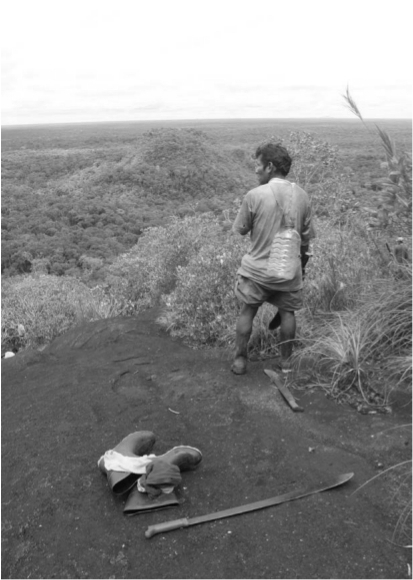
\includegraphics[width=\textwidth]{./img/005}
%\caption{Mandu avista a /Paç"-Tẽ̖h/, ``Serra"-Pequena'' (Foto Danilo P. Ramos, 2012)}
%\end{figure}

%\begin{center}\adforn{68}\end{center}

\section{Fotografias e escritos}\label{fotografias-e-escritos}

Eram muitos os pedidos para que eu tirasse fotos de todas as serras
distantes. Fizemos uma série de fotos com cada um à frente e as serras
ao fundo. Samuel e Lucas exploravam a câmera para tirar fotos de mim e
dos morros e rios à nossa frente. Com o pretexto de mostrar para a
família, registrávamos nossa presença nesse topo do mundo. Tiramos fotos
coletivas e fotos em \textit{particular}, como diziam.

Com a câmera fotográfica, tentávamos talvez reproduzir nossa presença,
entender melhor o que víamos e ordenar nossa experiência visual para
mostrar e contar histórias aos outros. A viagem e a fotografia permitiam
assim uma relação específica entre nós e o ambiente onde nos situávamos.

Samuel pegou uma lasca de pedra e começou a escrever no chão rochoso.
Aos poucos os riscos das linhas claras formaram letras e números,
compondo a frase: Paç Pö̗g 1.04.2012. Sua escrita foi seguida pela de
Natalino: Brasil Amazonas. Antes, não havia nada escrito nas pedras.
Todos os Hupd'äh de outras comunidades poderiam ver que os Hupd'äh de
\textit{Ta̗t"-Dëh}, únicos a passar por um processo longo de letramento, tinham
ido à Serra Grande. Saberiam também que os membros do clã \textit{Sokw'ä̗t Noh
K'öd Tẽ̖h}, majoritários nessa aldeia, tinham passado por lá. O ato de
escrita pode ser visto como um traço aditivo, nos termos de Ingold, já
que vai se formando uma camada sobre o substrato rochoso. Segundo o
autor, ``{[}\ldots{}{]} para o habitante, a linha de seu caminhar é um
percurso de conhecimento. Nesse mesmo sentido, a linha da escrita é,
para ele, um percurso de rememoração. E ambos os casos, o conhecimento é
integrado ao longo do caminho do movimento (2007, p.\,43)''.

Durante a viagem, em meio a nossas andanças, sempre que me mostravam um
animal, uma planta, um peixe ou diziam o nome de um lugar, eu os
escrevia em meu caderno de bolso ou no \textsc{gps}. Era comum que meu caderno
passasse de mão em mão, ou que fosse lido em voz alta e minhas anotações
comentadas e corrigidas. No final da tarde, assim como as narrativas
míticas e as histórias de caçaria, o \textsc{gps} e o caderno permitiam refletir
sobre nossas agências naquele percurso. No aparelho, víamos os nomes e a
posição dos lugares onde havíamos passado. Meus companheiros
interessavam"-se em comentar as distâncias percorridas e em relembrar os
lugares que me foram mostrados durante o trajeto. Nossas conversas
falavam menos de nosso transporte ponto a ponto pelas conexões e mais
das situações vividas. Falavam sobre o traço gestual de nosso movimento.
Assim, no contexto dessas conversas, a imagem do \textsc{gps} rememorava nossas
percepções ao longo de um percurso de observação e ajudava a integrar o
saber num modo não cartográfico.

%\begin{figure}
%\centering
%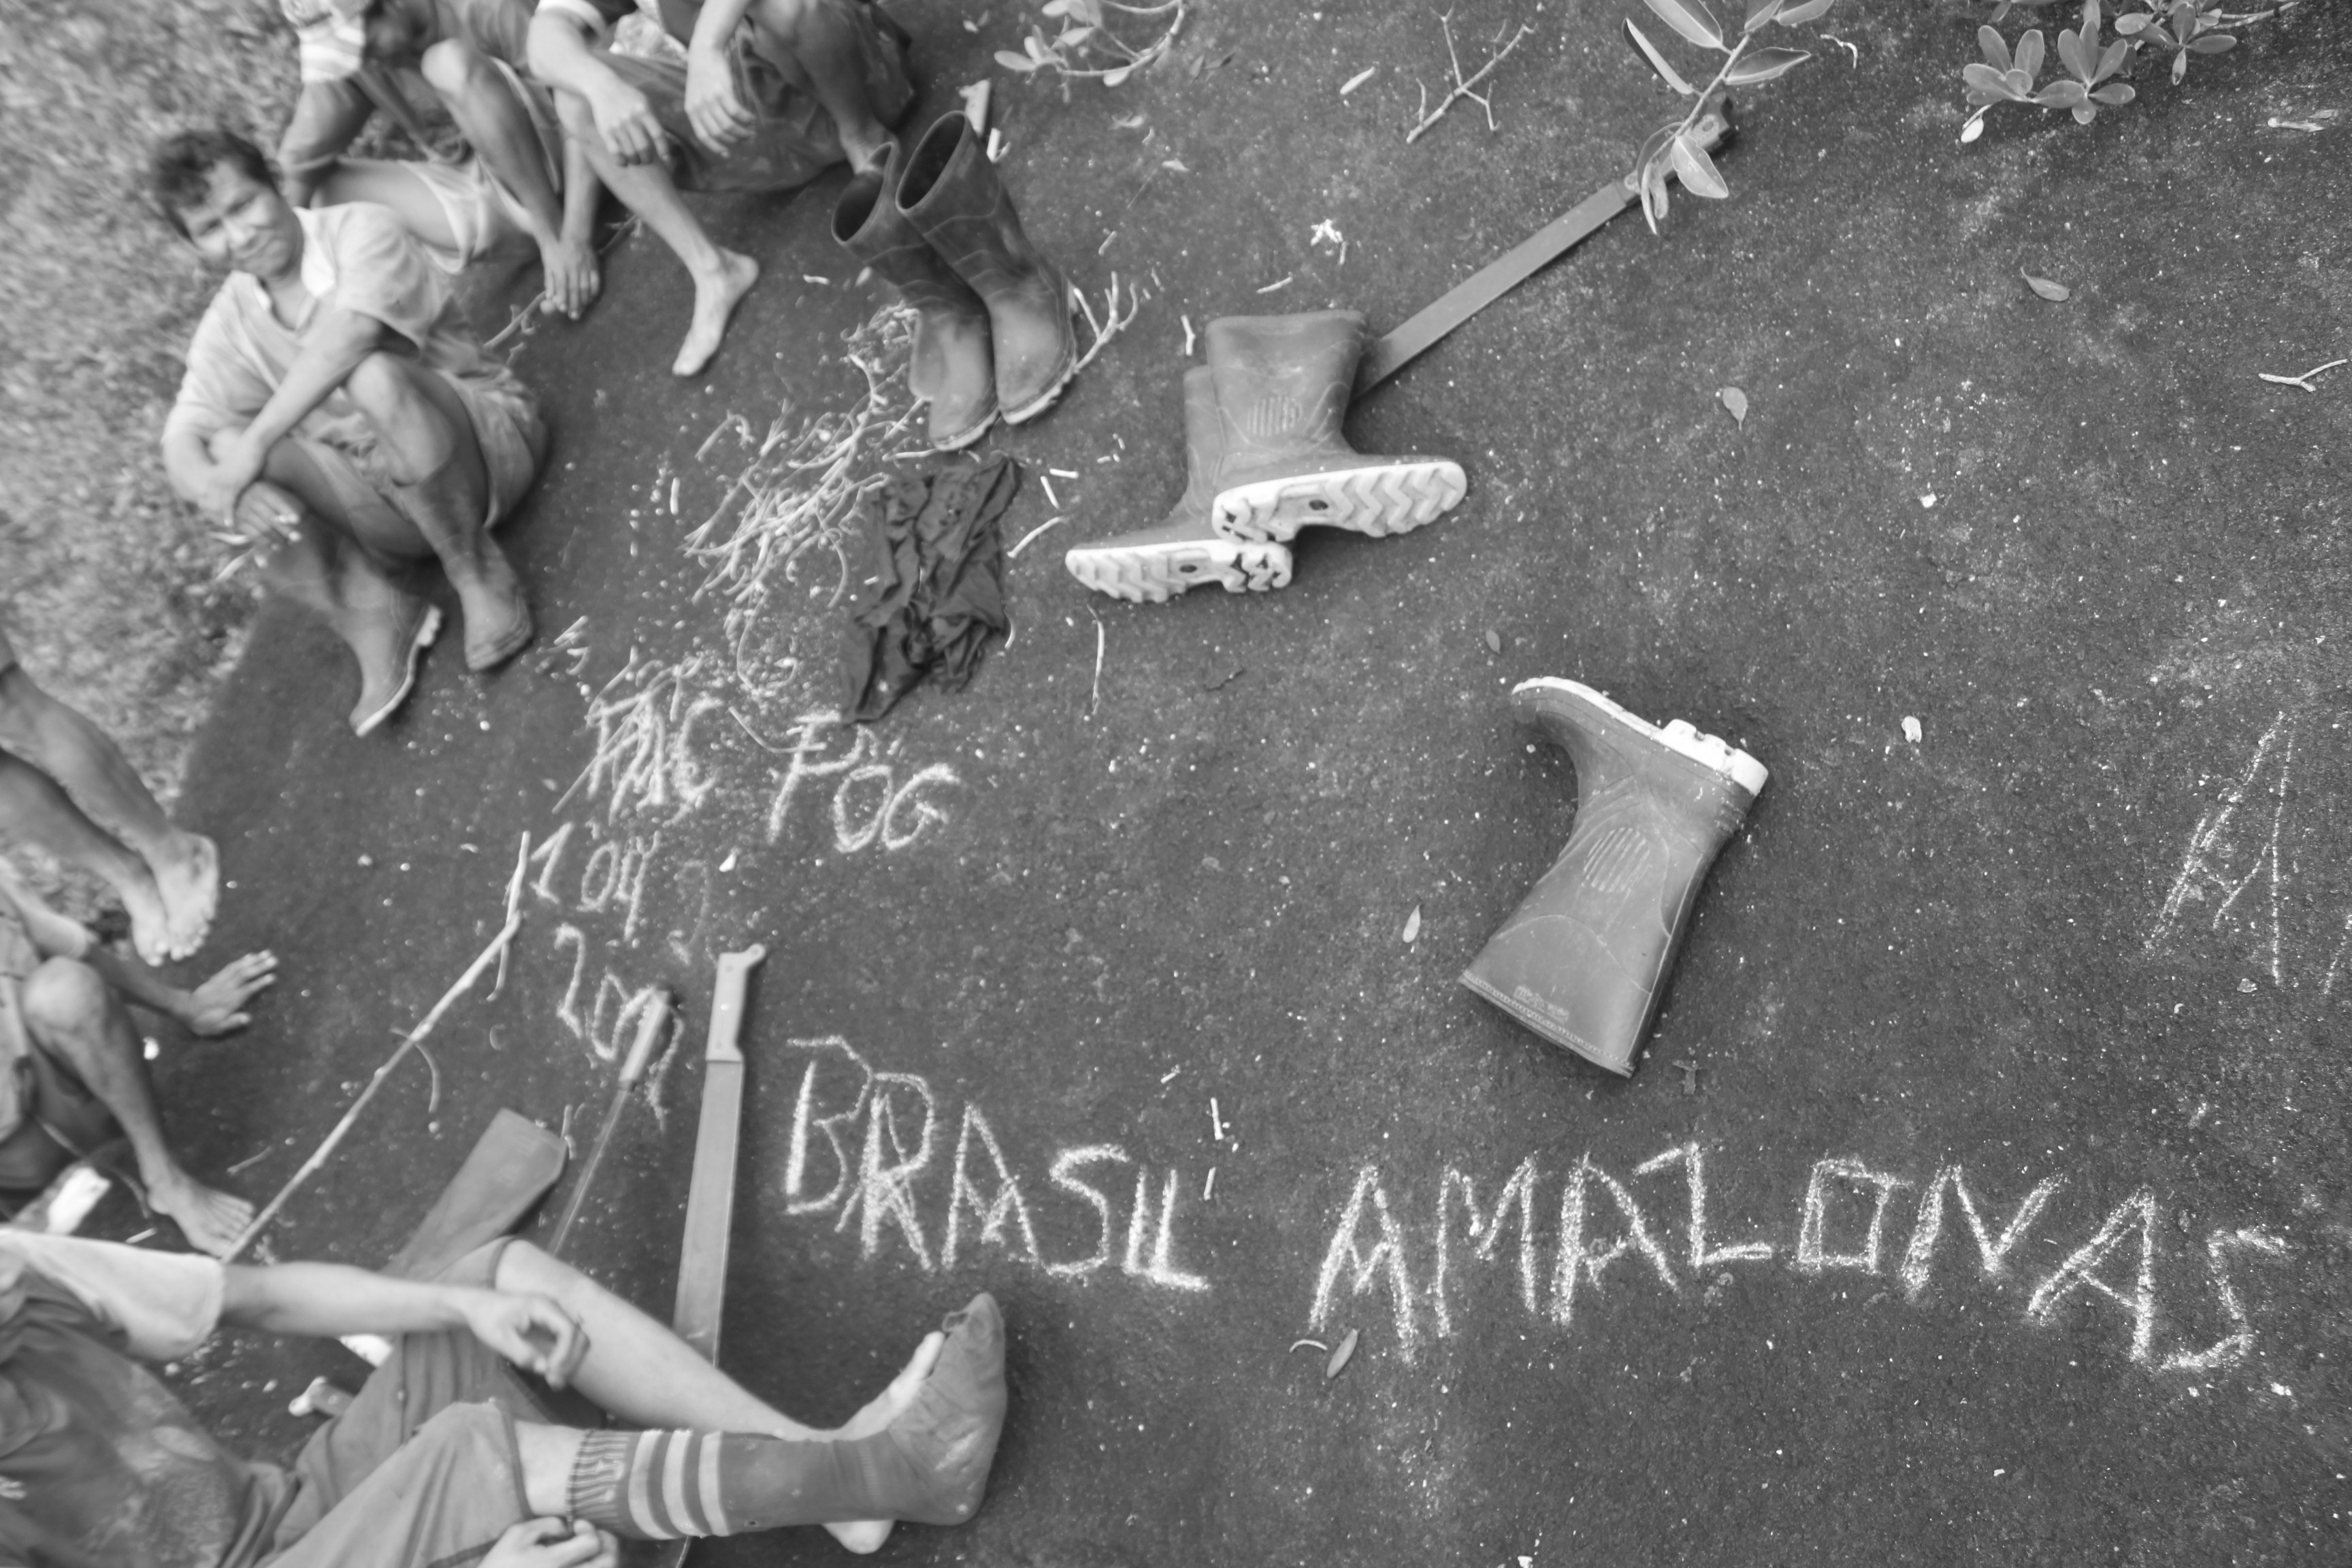
\includegraphics[width=\textwidth]{./img/006.jpg}
%\caption{Escritos na rocha (foto: Danilo P. Ramos, 2012)}
%\end{figure}

Como em relatos de viagem, a crônica do caderno, as linhas e pontos do
\textsc{gps} e as fotos permitiam ordenar a experiência, sendo modos de relembrar
caminhos e situações que iam se integrando através de nossos movimentos.
Naquelas superfícies, os escritos e traços situavam nossa viagem e nossa
presença por meio de aspectos temporais, espaciais e linguísticos.
Aproximados por essa longa caminhada da viagem à Serra Grande, os atos
de andar, escrever e fotografar proporcionavam modos de interação
específicos entre os viajantes e constituíam"-se como distintos caminhos
de rememoração.

\section{Lagos de banhar}\label{lagos-de-banhar}

Aproximando"-se da beira, Lucas respirou fundo, abriu bem a boca e lançou
um forte grito que se espalhou por todo o universo à nossa frente:
\textit{êêêêê}. As ondas sonoras reverberavam e espelhavam ecos: \textit{êêêêê}. ``Tem
gente ali, tem gente ali'', Mandu apontava para o meio da selva de onde
pareciam vir os ecos. A visão de longe, em perspectiva, era também uma
possibilidade de audição em perspectiva. Em seu grito e no comentário de
Mandu, de certo modo, a gênese da humanidade era retomada. (\textsc{m2})
No \textit{Pud"-dë̖h"-mo̗h}, no Lago de Leite, \textit{K'e̖g Tẽh} gritou e a humanidade
respondeu. E foi assim que surgiram os Hupd'äh, contou"-me Miguel em uma
roda de coca semanas antes.\footnote{Destaco algumas narrativas míticas
  do texto analítico"-descritivo com a letra \textsc{m} numerada.}
  \index{11@\textsc{m}2\quad O grito de \textit{K'e̖g Tẽh}}

Fomos, então, procurar pelos ``lagos'' ou ``poços de banhar'', \textit{s'o̗m ho̗y}, que
ficavam do outro lado do morro. Demétrio foi o primeiro a chegar. O lago
estava com água. Ele tirou suas sandálias, sua camiseta e foi para a
beira preparar"-se para o banho. Vagarosamente pôs"-se de cócoras, abriu
as palmas das mãos, movimentou"-as em direção ao espelho d'água,
umedeceu"-as e levou"-as para o peito, para o centro do sopro vital para
lavá"-lo.\footnote{\textit{hã̗wäg s'i̗d}, ``lavar o \textit{hã̗wäg}'' é uma ação comum aos
  encantamentos xamânicos.} Depois levou a água até seu rosto, braços,
pernas e pés, sempre de modo leve e delicado. Estava concentrado e
silencioso quando chegamos. Olhou para nós, sorriu e pediu que eu
tirasse uma foto dele se banhando. Todos começaram a tirar suas botas e
camisas e foram banhar"-se com a água do lago, um de cada vez. Quando fui
me banhar, explicaram"-me que havia dois lagos contíguos, um para o banho
das mulheres e o outro para o banho dos homens. Eu deveria molhar minhas
mãos no lago masculino para refazer meu corpo. Samuel fotografou"-me e
todos riram muito do \textit{banho do branco}.

``Se banhar, tem que voltar de novo, senão vai morrer já'', lembrava
Mandu enquanto nos lavávamos. As águas que refazem o corpo são as mesmas
que o deixam fraco e doente. Com o banho todos nós esperávamos ficar com
a pele dura, \textit{tab'a̗'}, como uma casca de árvore, com os ossos fortes e
com o corpo novo. Como disse Natalino enquanto banhava"-se, \textit{ɨ̗n pɨ̗b ĩh ni̗
tëg, wähä̗d nɨ̗h}, ``todos ficaremos jovens até a morte, não
envelheceremos''. Mas para isso tínhamos que retornar uma segunda vez à
Serra Grande e banhar"-nos novamente no lago. Lucas jogou um cigarro
dentro das águas. Como fiz menção de retirá"-lo, ele riu e contou que
estava deixando esse cigarro para os antigos, \textit{tɨ̗h wähä̗d'äh nɨ̖h hũ̖t}.
Era uma oferenda para aqueles que, como Demétrio, tinham ido muitas
vezes banhar"-se na Serra Grande. Entendo que essas ações realizam uma
\textit{fabricação do corpo}, uma intervenção sobre a matéria que recria o
corpo em banhos que são como passagens entre vida e morte.

%\begin{figure}
%\centering
%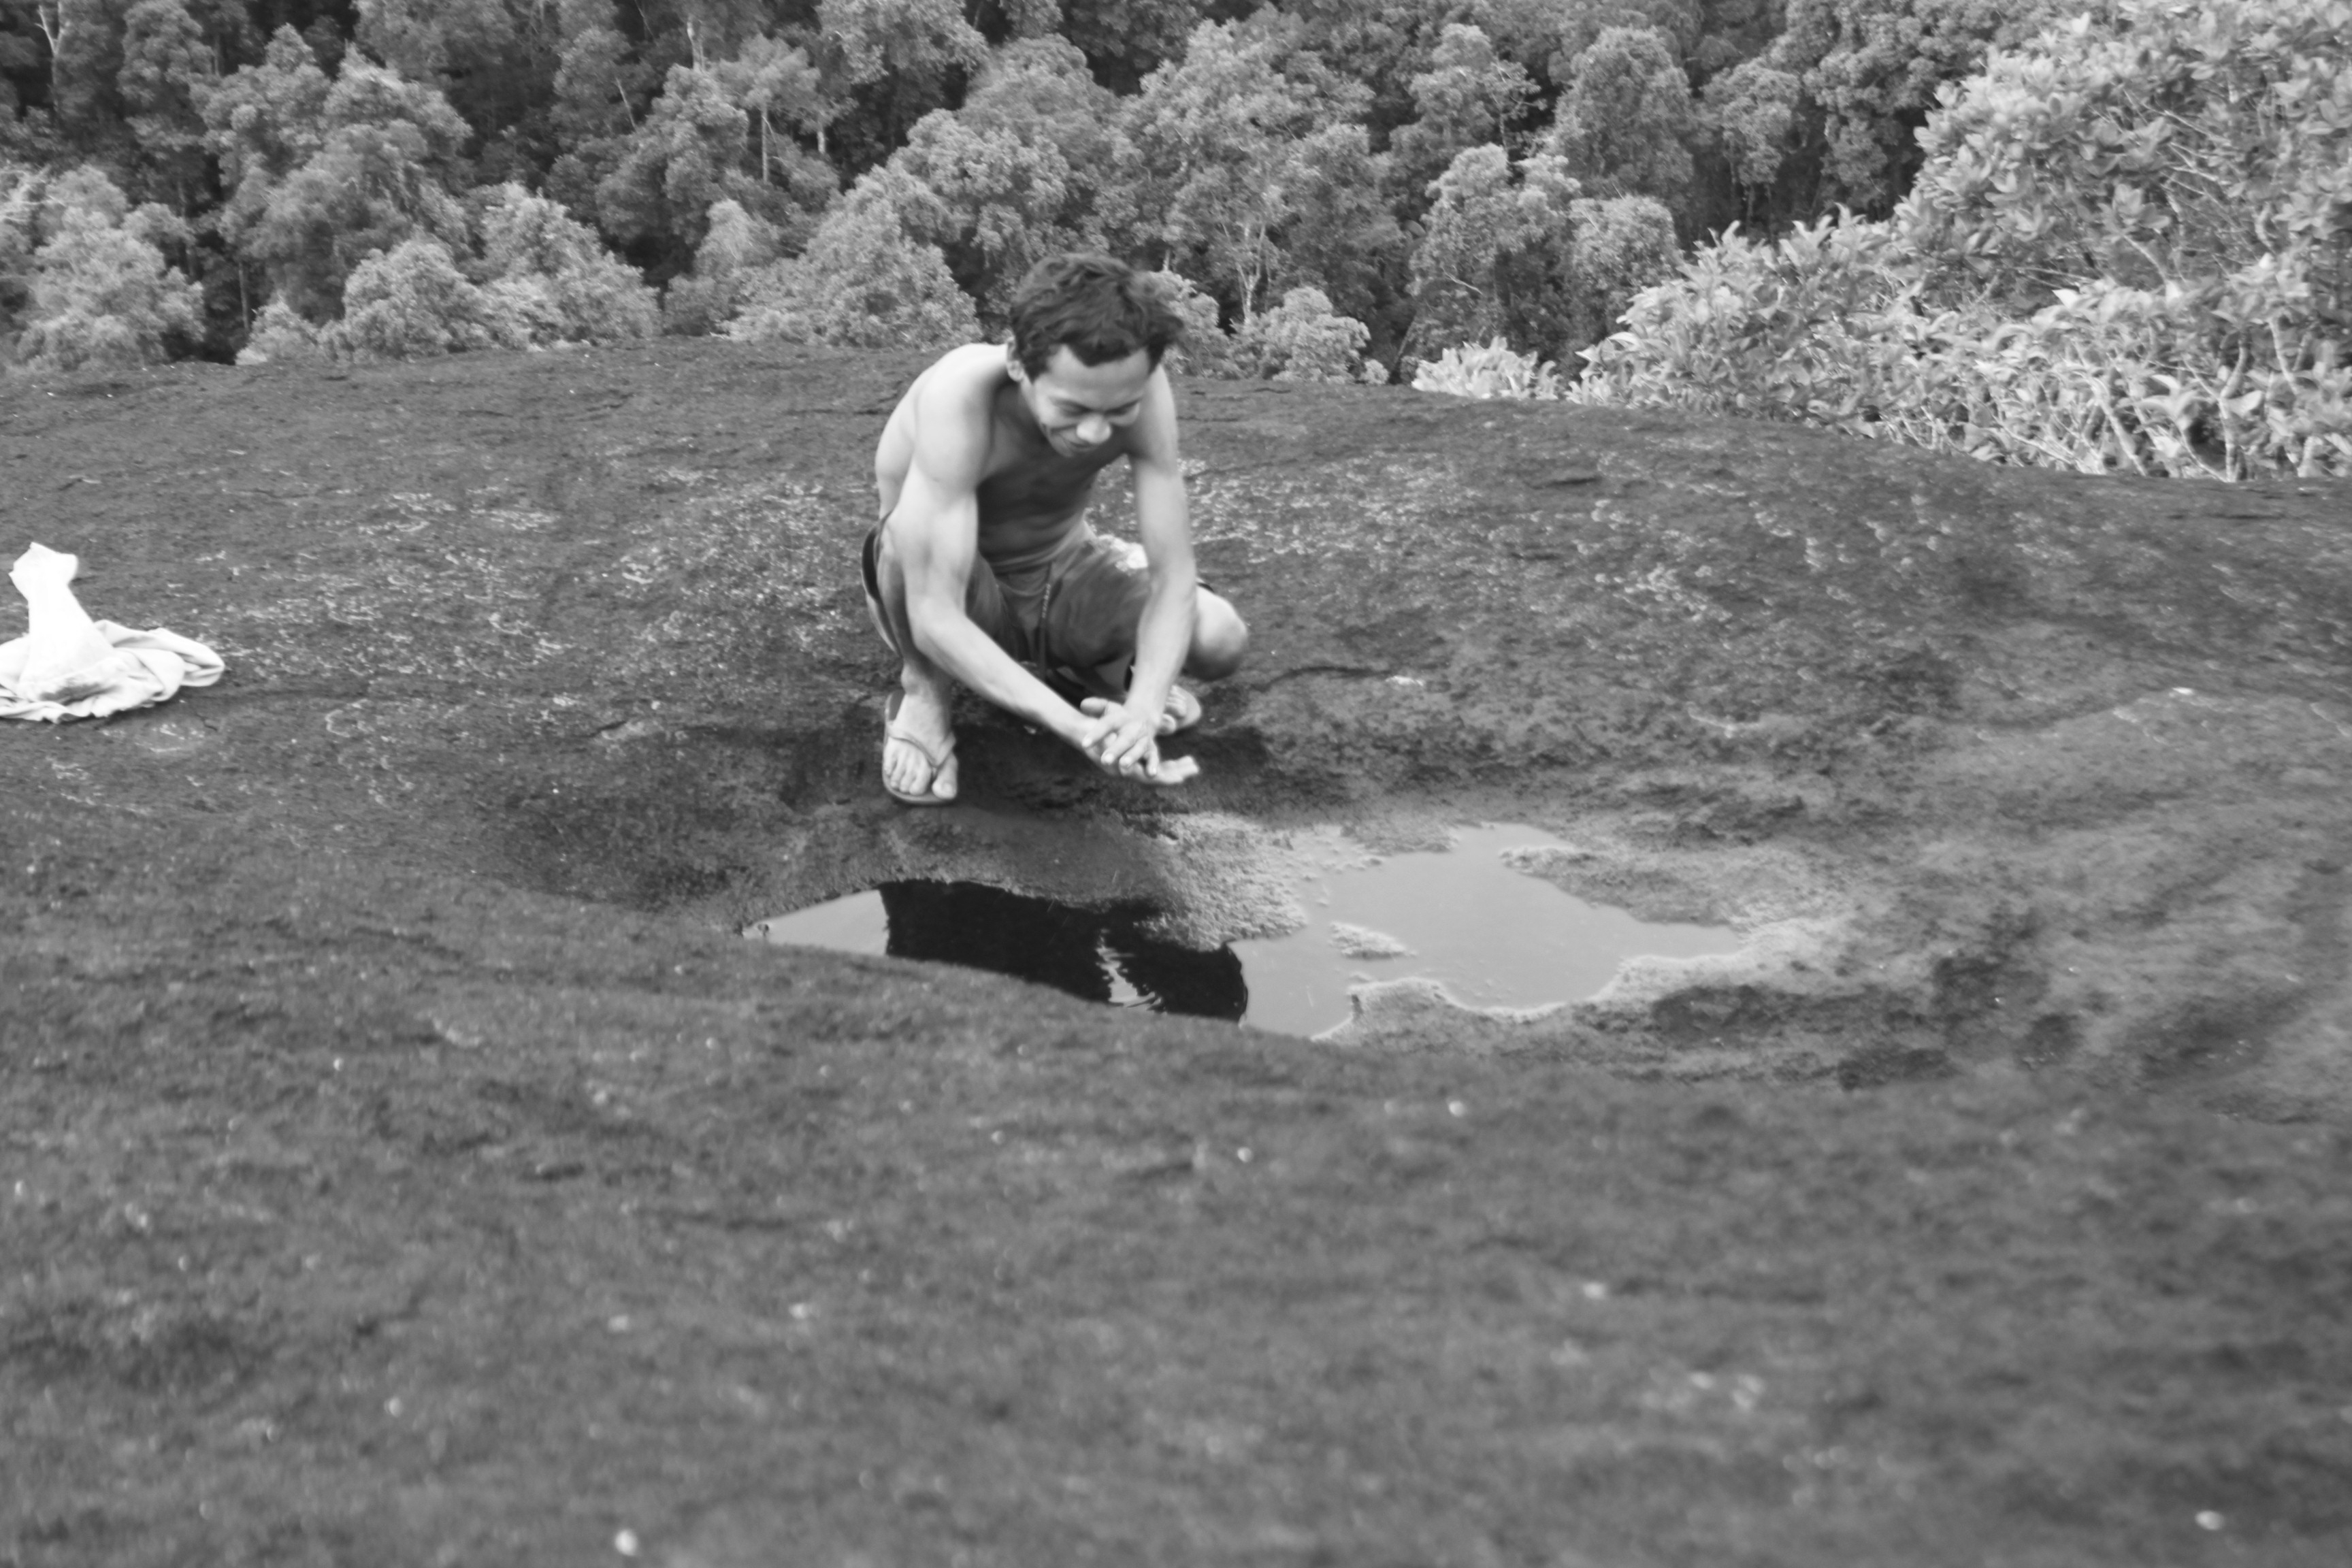
\includegraphics[width=\textwidth]{./img/007}
%\caption{Banho de Demétrio (foto: Danilo P. Ramos, 2012)}
%\end{figure}

Nosso \textit{kɨhsä̗t}, guia, falou dos pés de ``coca de abiu'', \textit{wahna̗w"-pũ'ũk},
que havia antes plantados na beira do lago. Um homem da aldeia de
\textit{Tõ̗h"-Haya̗m} arrancou"-os e levou"-os para sua comunidade. Preparou as
folhas dessa \textit{coca da origem} com cinzas de imbaúba e comeu"-as. Um
pouco depois ele passou mal e morreu. Nunca deveria ter retirado os pés
de coca da beira do lago. É por isso que hoje não há mais a coca no topo
da serra. Demétrio indicava com a mão o lugar preciso onde, antigamente,
havia a coca. Lembrava"-se de ter ainda visto os pés de coca certa vez em
que estivera lá com o pai, quando criança.

Em pé, perto do lago, ele nos levou até o ponto em que o padre Afonso
tinha colocado uma imagem de \textit{K'e̖g Tẽh}, Jesus, bem perto do lago.
Isso aconteceu na década de 1980, quando ele começou a trabalhar com o
pessoal de \textit{Ta̗t"-Dëh} e \textit{Tõ̗h"-Haya̗m}. O padre fez a viagem para a Serra
Grande com um guia e veio trazendo essa imagem de Jesus. Subiram o morro
e ele a colocou bem na beira do lago ou poço. Mas, tempos depois, pessoas
de \textit{Tõ̗h"-Haya̗m} vieram, tiraram a imagem e levaram"-na embora.

Com os banhos dos presentes e a enunciação de certas regras e
interdições começa a delinear"-se uma sequência articulada de ações que
são repetidas de forma semelhante por todos. Um processo de condensação
ritual passa a ocorrer através desses procedimentos que situam a busca
pela purificação do sopro vital e do fortalecimento do corpo. Se, ao
longo da viagem, modos de interação específicos com seres e lugares
puderam ser percebidos, creio que, no alto da serra, um jogo de
identificações com os antigos, com os diferentes seres e com elementos
presentes naquele espaço passou a ganhar maior densidade, situando uma
modalidade particular de ação. Nesse sentido, as narrativas do \textit{homem
que arrancou os pés de coca}, do \textit{padre que colocou uma imagem
cristã} e dos \textit{soldados que fugiram} podem ser vistas como falas que
contrastam com o modo de atuação dos presentes, mostrando os perigos e
decorrências de atuações indevidas. São também falas sobre as tensões e
disputas entre diferentes seres em interação (os ancestrais, as pessoas
de diferentes clãs, os padres, os soldados etc.) que situam suas
disputas naquele lugar. Já a analogia possível entre o ``chamado de
Lucas'' e o ``chamado de \textit{K'e̖g Tẽh}'' (\textsc{m2}) no surgimento da
humanidade permite entender a percepção da paisagem como lócus de uma
cosmogênese. Desse modo, o fortalecimento do corpo, a purificação do
sopro vital, a atenuação do envelhecimento e a morte iminente apontam
para a importância do modo de interação com esse espaço em termos de
ações ritualizadas.\index{11@\textsc{m}2\quad O grito de \textit{K'e̖g Tẽh}}

\section{Venenos e descida}\label{venenos-e-descida}

Reparei nas folhas de um arbusto que, para mim, eram muito parecidas com
as folhas de coca. Samuel disse que o nome da planta era \textit{tẽh na̖m},
veneno para não ter criança. Do ponto onde estávamos, avistamos também
os dois outros morros que formam o complexo da Serra Grande, a
\textit{Paç"-Tẽ̖h}, Serra"-Pequena, e a \textit{Tõg"-Tẽg}. É no alto da Serra Pequena
que cresce um outro veneno, fundamental para a prática da caça, o \textit{hũ
na̖m} ou curare\footnote{O curare é extraído de espécies da família
  vegetal \emph{Menispermaceae}, comum na Amazônia, sendo
  \emph{Chondrodendron} e \emph{Curarea} os seus gêneros principais.}
(\emph{Menispermaceae}), veneno para matar animais. Um mês antes,
Ponciano havia me mostrado o pote de cerâmica onde guardava seu curare e
contou"-me uma narrativa sobre o surgimento do curare.

%\begin{center}\adforn{68}\end{center}

\index{12@\textsc{m}3\quad \textit{K'e̖g Tẽh} e o aparecimento do curare}
\begin{quote}
\mito{3}{\textit{k'e̖g tẽh} e o aparecimento do curare}

Certa vez, \textit{K'e̖g Tẽh} pegou sua flecha e foi caçar. Foi caminhando pela
mata, até que ouviu dois tucanos no alto de uma árvore. Ele parou,
imitou o som que eles faziam, armou seu arco e atirou. Acertou"-os no
bico e ambos caíram mortos no chão.

Como ele estava com muita fome, devorou"-os logo. Mas a carne das aves
fez"-lhe mal e ele começou a vomitar. Seu vômito espalhou"-se pelo mundo e
foi cair em três serras. Uma delas é a \textit{Paç"-Tẽ̖h}, Serra Pequena.

De seu vômito apareceu o \textit{Na̖m tɨ̗t}, o cipó com o qual se prepara o
veneno para matar animais. ``Não dá pra plantar, não. Só nasce o curare
nesses lugares onde ele vomitou, mesmo''.
\end{quote}

Estávamos sentados numa roda de coca e Ponciano apontava para o sul e
para o norte com os braços, indicando os lugares onde \textit{K'e̖g Tẽh} havia
vomitado. No evento narrado,\footnote{Incorporo o princípio analítico da
  etnografia da \emph{performance} de distinguir entre os eventos aos
  quais a \emph{performance} está se reportando: eventos narrados; e os
  eventos de atuação do narrador: eventos narrativos (Bauman, 1977).} a
caça situa o modo de interação entre o demiurgo e os animais, sendo que
o não preparo apropriado do alimento para o consumo ocasiona a
indigestão e o vômito. Caindo em lugares específicos, o vômito faz
aparecer o cipó de curare, fundamental para a interação com os animais
na prática da caça.

O veneno é conservado como se fosse uma cera que é passada, com muito
cuidado, na ponta da flecha. A princípio tínhamos pensado em tirar
curare para prepararmos o veneno, mas, quando conseguimos chegar à Serra
Grande nossa farinha já estava terminando e, por isso, desistimos. A
retirada e preparo do curare são muito perigosos. Miguel contara em uma
festa de caxiri, semanas antes, que aquele que colhe não pode ter
nenhuma ferida, pois qualquer contato do corpo com a substância venenosa
é fatal. Por isso, a colheita é demorada e exige muita atenção e
coragem. Corta"-se um pedaço do cipó, raspa"-se a casca e depois se
mistura a raspa com água. Leva"-se ao fogo quando o sol nasce e deixa"-se
a mistura fervendo até que a noite chegue. A solução pastosa é então
guardada em potes de cerâmica que conservarão seu potencial mortífero
por muitos anos. Miguel referiu"-se à enorme quantidade de cipós que
podem ser encontrados pelo chão na Serra Pequena. Sempre que um homem
vai percorrer caminhos para caçar, pescar ou visitar parentes de outras
comunidades, ele leva seu curare e uma flecha envenenada. Hoje em dia,
como poucos vão às serras retirar a raspa de cipó, aqueles que conseguem
retirá"-la e preparar o curare podem realizar boas trocas com parentes
por bens ou dinheiro. Como disse Mandu, ``se nossa farinha não estivesse
acabando, íamos tirar curare para trocar. Paga caro esse curare!''.

Em língua hup, a palavra \textit{na̗m} é usada tanto para esse veneno de caça
quanto para a planta abortiva que apontei para Samuel. No alto dos
morros crescem essas plantas para envenenar animais, \textit{hũt na̗m}, e para
envenenar o filho, \textit{tẽh na̗m}. Dotam a humanidade da capacidade de matar
envenenando. Se é \textit{K'e̖g Tẽh} quem traz a vida à humanidade através de
seu chamado (\textsc{m2}), é ele também quem faz surgir o veneno
(\textsc{m3}), meio de causar a morte.
\index{11@\textsc{m}2\quad O grito de \textit{K'e̖g Tẽh}
\index{12@\textsc{m}3\quad \textit{K'e̖g Tẽh} e o aparecimento do curare}}

A descida foi rápida. Pegamos nossas coisas e partimos apanhando as
raízes do arbustos e lançando nossos corpos para baixo. Todos me
ajudavam a refazer o caminho por entre as fendas e rastros d'água. Em
quinze minutos chegamos ao pé do morro, quando tínhamos demorado pelo
menos meia hora para a subida. Cansados e sedentos, bebíamos a água com
limão de nossa garrafa. Ninguém bebeu da água do morro. Tampouco
consumimos a água do lago ou poço. Já em nosso acampamento, preparando as
coisas para partir, Mandu contou que da próxima vez voltaríamos com o
\textit{sä̗w}, ``pajé'', e daí poderíamos beber a água. A água é muito forte.
Quando se bebe, é preciso que um pajé ou \textit{kä̖d hup ĩh}, ``xamã do
banco'', esteja junto, pois a pessoa tem muitos sonhos. Seu sopro vital
viaja para muitos lugares e, se não estiver protegida, pode correr
perigo.

A Serra Grande pode ser percebida como uma paisagem de mediação
fundamental entre a vida e a morte. Nesse lugar central para o mundo
vivido dos Hupd'äh, os movimentos e gestos dos viajantes revelam um modo
específico de interação com os elementos e seres ali presentes. Evitar
beber a água, lavar o corpo com o líquido da metade masculina do lago,
contar narrativas sobre o lugar, retomar a disputa com o padre e com os
soldados, salientar a necessidade do retorno, a extração do curare,
todos esses atos podem ser vistos como ações ritualizadas que marcam um
processo de condensação de modos de relação dos presentes entre si e
deles com outros seres e com o ambiente onde interagiam. Caminhos de
rememoração, a escrita na rocha, as linhas do \textsc{gps} e a fotografia
justapunham"-se às ações ritualizadas possibilitando diálogos futuros e
ordenações da experiência presente.

%\begin{center}\adforn{68}\end{center}

\section{Caminhos vividos}\label{caminhos-vividos}\label{no-caminho}

%\subsection{No caminho}

Conforme nos distanciávamos da serra, ouvíamos ecoar um barulho muito
alto. Era como se um grito seguisse em nossa direção. Samuel apertava o
passo à minha frente. Com receio do barulho, começamos a correr pela
trilha. Estávamos assustados. Quando conseguimos nos distanciar e
encontrar os outros, paramos para descansar. \textit{Dö̗h A̗͂y hõ̗h, Danilo! Dö̗h A̗͂y
hõ̗h yo'o̗m}, ``o grito da Dö̗h A̗͂y, era o grito da Dö̗h A̗͂y, Danilo! É
muito perigoso, ela tava chamando, queria pegar você. Fica brava quando
brancos vêm à \textit{Paç"-Pö̗g}'', ele contou. Estava pálido. Todos os outros,
com o semblante tenso, riram do que ele nos contava.

Samuel falava rindo que a \textit{Dö̗h A̗͂y} tem uma vagina muito grande. É
preciso tomar cuidado, pois ela \textit{vem pegar}. Lembrava"-se da história
contada por seu pai, Ponciano, dias atrás numa roda de coca.

%\begin{center}\adforn{68}\end{center}

\index{13@\textsc{m}4\quad A \textit{Dö̗h Ã̗y} e seu marido}
\begin{quote}
\mito{4}{a \textit{dö̗h ã̗y} e seu marido}

A \textit{Dö̗h Ã̗y} tinha um marido, um homem hup. Eles tinham dois filhos, um
menino e uma menina. Só que ela tinha uma vagina muito grande. O pênis
do marido era pequeno demais e não chegava. Ele sempre tinha muita dor
no pênis e muita dor quando comia pimenta.

Um dia, ele se escondeu na mata e ficou esperando a mulher sair para a
roça com seu aturá pequeno. Quando ela chegou perto, ele a surpreendeu e
a matou.

Mas ela renasceu e, quando ele foi para o rio se banhar, ela vestiu sua
roupa de \textit{Dö̗h Ã̗y}, matou"-o e comeu"-o. Ela, então, encontrou um outro
companheiro, o \textit{Kuku̗i}, o Macaco"-da"-Noite. Ele tem um pênis grande e
hoje em dia ela vive com ele, ela e seus filhos.\footnote{Caderno de campo, 
23 de fevereiro de 2012.}
\end{quote}

Naquela noite, Ponciano e todos que ouviam essa história riam muito,
principalmente quando ele mostrava com as mãos o tamanho do pênis dos
maridos e o quão grande era a vagina da \textit{Dö̗h A̗͂y}.\footnote{No português
  falado pelos Hupd'äh, \textit{Dö̗h A̗͂y} é traduzida como Curupira muito
  provavelmente por sua ação protetiva com relação a animais.} Quando
Samuel se lembrou da história, todos nós rimos também e o medo diminuiu.
Na narrativa, a \textit{Dö̗h A̗͂y} surge como uma mulher com uma vagina grande que
gera dor em seu marido. Ele a mata, mas ela renasce, veste sua roupa de
\textit{Dö̗h A̗͂y}, assassina e devora seu marido. Depois, casa"-se com o
Macaco"-da"-Noite, que tem um pênis grande. O riso de Ponciano e Samuel
nos eventos narrativos é provocado pelo tamanho avantajado da vagina da
mulher relacionar"-se a uma atitude sexual insaciável, suprida pelo pênis
grande do Macaco"-da"-Noite. Mas, também no plano da comensalidade ela se
revela insaciável, já que, tendo matado seu marido, ela o devora depois
que veste sua roupa. Devoradora de gente e principalmente de homens, a
\textit{Dö̗h A̗͂y} é vista como uma grande ameaça, como uma predadora que gera
medo e terror àqueles que começam a ouvir seu chamado. Assim, \textit{Dö̗h A̗͂y},
gritando no alto do morro, estava chamando sua presa, no caso meus
companheiros e eu.

\index{1@\textsc{m}1\quad A pescaria do \textit{b'atɨ̖b'}\break(história de \textit{b'atɨ̖b'})}
Em \textsc{m1}, o \textit{b'atɨ̖b'} também \textit{chama} seu cunhado para a pescaria
por duas vezes. Na primeira, ele aceita o chamado e segue com o
\textit{b'atɨ̖b'} para pescar sarapós, mas atemoriza"-se e abandona o companheiro
depois de ver que as onças eram traíras de \textit{b'atɨ̖b'}. Na segunda, ele
atende ao chamado para depois fugir definitivamente com sua irmã. Em
\textsc{m2} e \textsc{m3}, é o chamado de \textit{K'e̖g Tẽh} que faz surgir a
humanidade e aparecerem os tucanos para serem abatidos. O ato de chamar
a presa pode ser visto como um ato comum a diversas situações de caça e
revela uma espécie de diálogo interpessoal. As descrições de mais
algumas situações que presenciei durante a caminhada daquele dia podem
ajudar a entender a importância desses chamados na relação com outros
seres.\index{11@\textsc{m}2\quad O grito de \textit{K'e̖g Tẽh}}\index{12@\textsc{m}3\quad \textit{K'e̖g Tẽh} e o aparecimento do curare}

Mandu seguiu na frente quando retomamos o caminho. Íamos num passo
ritmado percorrido a trilha que tinha a largura exata de nossos corpos.
Por vezes, apenas as hastes partidas de uma folha delineiam os traços na
mata. Começamos a ouvir o canto de um \textit{yë̖ç}, ``jacu''.\footnote{Ave da
  família dos cracídeos, \emph{Penelope jacquacu}. Cf. Ramirez (2006).}
O som foi tornando"-se mais alto a cada passo até que o caçador parou.
Com seu corpo imóvel, ele levou as mãos à boca para imitar o jacu.
Estava chamando a ave. Ficamos assim imóveis por alguns minutos até que
ele entendeu que o animal já tinha ido embora. Mais adiante, ouvimos o
som de um casal de \textit{meme̗ç}, ``jacamins''.\footnote{Ave da família dos
  psofídeos, \emph{Psophia crepitans}. Cf. Ramirez (2006).} Postando"-se
novamente imóvel, ele imitou o canto dessa outra ave e logo concluiu que
ela já tinha voado também. Ele levava um \textit{töw tëg}, um socador de pilão
de coca que encontrara às margens do \textit{Dö̖g"-Dëh}, Igarapé"-Uirapixuna. Essa
era também sua arma. Caso uma onça surgisse, ele bateria nela até
matá"-la.

Em língua hup, diz"-se \textit{hũ̗ ë̖yë̗y}, ``chamar a presa''ou ``animal'', para
designar essa atitude do caçador de imitar o som do animal para fazer
com que ele se aproxime ou não fuja com a aproximação do caçador. A
pessoa geralmente para, volta o corpo para o lugar de onde vem o canto
ou barulho do movimento do animal, leva as mãos à boca e cria um
aparente aerofone para emitir sons que se assemelhem aos emitidos pelo
animal em sua ``fala'', \textit{ɨ̗d}, ou ``canto'', \textit{ya̗m}. Em \textsc{m3}, para caçar os
tucanos, \textit{K'e̖g Tẽh} também chama a presa que surge para ser abatida por
sua flecha. Também a atitude de \textit{Dö̗h A̗͂y} e a do \textit{b'atɨ̖b'} (\textsc{m1})
podem ser vistas como \textit{chamados à presa} que, nesses casos, são
humanas.\index{12@\textsc{m}3\quad \textit{K'e̖g Tẽh} e o aparecimento do curare}
\index{1@\textsc{m}1\quad A pescaria do \textit{b'atɨ̖b'}\break(história de \textit{b'atɨ̖b'})}

\index{12@\textsc{m}3\quad \textit{K'e̖g Tẽh} e o aparecimento do curare}
O momento de encontro entre caçador e presa pode ser percebido como
propício para o estabelecimento de um diálogo entre humano e animal por
meio do qual um toma o ponto de vista do outro, entendo que Mandu e
\textit{K'e̖g Tẽh} (\textsc{m3}), realizando imitações sonoras dos animais para
chamá"-los, buscam alterar suas posições no contexto de diálogo com as
presas. Nesse sentido, o \textit{b'atɨ̖b'} (\textsc{m1}), chamando seu cunhado,
está também chamando a presa, já que altera os contextos de diálogo com
as substituições\footnote{Há nessas transformações algo semelhante ao
  que Roy Wagner estabelece como sendo um processo de obviação
  (\emph{Obviation)} enquanto fluxo de metáforas substitutivas
  constituindo a trama de um mito ou ritual num movimento dialético que
  se fecha no ponto inicial (1986, p.\,xi, trad. minha).} do sarapó pela
traíra e depois da onça pelos humanos. Ao vestir sua roupa, \textit{Dö̗h A̗͂y} em
seu modo de interagir com o marido, também altera sua posição para
devorá"-lo.

Os Hupd'äh dizem que o animal ``surge'', ``aparece'', \textit{hũ̗ baha̗d},
estabelecendo"-se assim um diálogo interpessoal entre as partes. A
analogia com o chamado de \textit{K'e̖g Tẽh} (\textsc{m2}) na gênese da
humanidade faz pensar que, ocupando posições nesse contexto dialógico,
humanos e animais passam a existir, surgem reciprocamente uns para os
outros.\index{11@\textsc{m}2\quad O grito de \textit{K'e̖g Tẽh}}

Durante esses dias de caminhada, muitos foram cortando paus com os quais
fizeram ``varas de pesca'', \textit{hõp käk su̗k}. Ao longo das margens do
igarapé cada pescador distribuía suas varas em pontos diferentes.
Olhavam"-nas de tempos em tempos para ver se haviam fisgado algum peixe.
Enquanto vão de um lado ao outro tirando os peixes, os pescadores
comunicam"-se através do som da ave \textit{popo̗ hup}.\footnote{\textit{Popo̗},
  ``uru"-corcovado'', certo tipo de ave pequena da família dos
  fasianídeos, \emph{Odontophorus guianensis}. Cf. Ramirez (2006).}
Colocando as duas mãos diante da boca, moldam"-nas de modo a obter um
assobio semelhante ao da ave. Quando um assobia o outro responde,
exatamente como a ave faz na mata. Samuel contou que quando a ave canta
eles têm medo, pois ela é gente também. Nesse ato de chamar, pela
imitação do canto da ave, os pescadores hup se comunicam como se fossem
aves \textit{popo̗ hup}. A metáfora revela uma espécie de metamorfose dos
humanos para ocuparem posições nesse outro contexto de diálogo. Já o
encontro ou interação entre a ave e os humanos pode ser perigoso, pois o
\textit{po̗'po̗ hup} é gente também. Os pescadores interagem entre si a partir da
posição e do ponto de vista de outro ser, o que lhes garante a
comunicação, a ciência da localização do companheiro e uma espécie de
camuflagem que, por meio dessa \textit{roupa sonora}, os protege da ameaça de
outros seres.

\textit{Ha̗ma̗y, sät, ha̗ma̗y!} é o modo como qualquer um dos viajantes convocava
os outros para, após uma parada, retomar o caminho. \textit{Vamos, irmão
maior, vamos} ou \textit{vamos, velho, vamos} é talvez a forma como esse
vocativo, que chama para uma ação, pode ser traduzido. A mesma ação pode
ser iniciada ou convocada por qualquer pessoa, sendo que o ato de
convocar não exime a pessoa de sua realização. Chamar alguém para fazer
algo ou começar uma ação que será seguida por outros faz da pessoa um
\textit{kɨhsä̗t}, ``o primeiro'', ``o que começa'' ou ``o que chama''. E foi
Samuel o \textit{kɨhsä̗t} a preparar nossa refeição noturna. Naquela noite,
havia muitos peixes, moqueados e cozidos. Todos estavam preparando seus
\textit{kaba̗w}, trouxas feitas com folhas de palmeiras com peixes ou carne
moqueada dentro, para levar para seus familiares. Os \textit{kaba̗w} são
ansiosamente aguardados por todos, principalmente pela esposa e filhos
do viajante. Enquanto preparava as lenhas para cozinhar a mojeca, Samuel
perguntou se eu já tinha ouvido a \textit{história do besouro e do
vaga"-lume}. Ele então começou a contar"-me essa triste história de dois
companheiros de caminhada.

\begin{quote}\index{14@\textsc{m}5\quad O Besouro e o Vaga-Lume}
\mito{5}{o besouro e o vaga"-lume}

O Besouro estava tinguejando no igarapé. O Vaga"-lume chegou e perguntou:
\textit{O que você está fazendo?}, e ele respondeu \textit{Eu estou tinguejando no igarapé},
respondeu o outro. Ele havia conseguido pegar muitos dos peixes que
morreram.

Era por volta de umas cinco e meia da tarde. Ainda havia sol no céu quando o
Vaga"-lume voltou e chamou o Besouro para ir mais adiante com ele. Ele
disse que iria depois, e pediu"-lhe para esperar um pouco. O Vaga"-lume
disse que ia iluminar o caminho. Os olhos dele são lanternas. Ele
acendeu o corpo três vezes.

Então o Besouro amarrou o peixe com cipó e concordou em ir mais acima
com o companheiro. Eles foram juntos. Andaram muito e, de repente, a
lanterna apagou"-se. Anoitecera e o Besouro não via nada. \textit{Eu não vejo o
caminho}, ele disse.

O Vaga"-lume foi embora e deixou o companheiro no meio da mata, sozinho.
O caminho não aparecia. Tudo era escuridão. Acabou a história.
\end{quote}

Analisando as práticas de caça dos Hupd'äh, Reid diz que ``conforme a
luz diminui, os caçadores se encaminham para a trilha e, caso esteja
muito escuro, poderão ter de \textit{sentir} o caminho de casa''. Sem seu
parceiro, o Besouro teria, como o caçador hup, que intuir o caminho de
volta. Seja para começar a pescaria, seja para preparar o acampamento, a
refeição ou pegar lenha, sempre havia uma pessoa que era o \textit{kɨhsä̗t} da
ação, o que começa, o que chama a ação. No evento narrado, o Vaga"-lume
surge como o \textit{kɨhsä̗t}, o que ``chama a ação'', convidando o Besouro para
ir mais adiante. Num primeiro momento, o Besouro não aceita o chamado e,
num segundo momento, o Vaga"-lume abandona o companheiro. A narrativa
torna"-se especialmente interessante para pensar essa relação. Espera"-se
que o \textit{kɨhsä̗t}, ao chamar uma ação, seja seguido e, do mesmo modo,
aquele que inicia uma ação deve conduzi"-la até sua conclusão junto com
aqueles que o seguem.

Demétrio, o maior conhecedor do caminho, foi sempre o que esteve à nossa
frente, agindo, portanto, como nosso guia, nosso \textit{ti̖w kɨh sä̗t}. Mas
sempre consultava Mandu por ser ele o mais velho do grupo, o \textit{kɨhsä̗t
wähä̗d}. Samuel, por ser filho de Ponciano, o principal dono de
\textit{Ta̗t"-Dëh}, era também um \textit{kɨhsä̗t}. Todos aqueles que seguiam o \textit{kɨhsä̗t}
em sua ação eram chamados de \textit{huy ham d'äh}, ou
``acompanhantes'', ``seguidores''. Há, assim, e isso será retomado mais à
frente, um princípio comum mais fluido no nível da ação e mais rígido em
termos de posição na estrutura social.

Mas, voltando ao ``chamado da \textit{Dö̗h A̗͂y}'', ao ``chamado dos animais'' e
ao ``chamar como \textit{popo̗ hup}'', pode"-se entender a importância de saber
posicionar"-se nesses contextos de diálogo e de estar ciente do perigo
que uma pessoa pode correr caso, ao atender a um chamado, ocupe o lugar
de presa, como no caso do homem hup e seu cunhado, o \textit{b'atɨ̖b'}
(\textsc{m1}). Na interação entre o Vaga"-Lume e o Besouro, o primeiro
pode ser visto como um \textit{kɨhsät} por chamar a ação e por iluminar o
caminho. Não atendendo ao chamado de pronto, o Besouro revela"-se um mau
\textit{acompanhante}, restando sozinho em meio ao breu da noite, sem saber
como continuar o percurso.
\index{1@\textsc{m}1\quad A pescaria do \textit{b'atɨ̖b'}\break(história de \textit{b'atɨ̖b'})}

%\subsection{Caminhar}\label{caminhar}

%\begin{center}\adforn{68}\end{center}

% \begin{flushright}
% \textsc{28 de março de 2012}\\
% \textit{Caminhar}\label{caminhar}
% \end{flushright}
% \smallskip

\section{Caminhar}

O dia estava bom para viajar. Samuel veio logo cedo à casa de Américo
para dizer que a chuva parara e que podíamos sair. Fomos, então,
preparar as coisas para a viagem. Era preciso verificar tudo. Lanternas,
terçados, roupas, farinha, anzóis e linhas, arco e flecha, rede e
cordas, tudo precisava ser revisto para que passássemos bem durante os
sete dias de caminhada previstos. Enfrentaríamos uma trilha com \textit{ti̗ti̗},
``lama suja'' no dizer de meus companheiros. Os dias anteriores tinham
sido de muita chuva e, por isso, todos iam com suas botas calçadas. A
chuva faz as cobras, as jararacas, saírem de suas tocas. ``É um
sopro\footnote{Nesse caso, a palavra \textit{dö̗h}, ``sopro'', designa a ação
  xamânica realizada com o intuito de prejudicar outrem, algo como o
  feitiço.} do Trovão. É ele quem faz as cobras saírem para nos
morder'', alertara Miguel dias antes. Eu ainda tinha que preparar os
cadernos de bolso, o \textsc{gps}, a câmera fotográfica e as pilhas.

Os viajantes vieram todos à casa de Américo, onde eu estava. Sentamos,
conversamos, comemos fumamos juntos. Acertamos os últimos detalhes da
viagem. ``Vamos comer bem na mata, o Demétrio é bom caçador. Ele vai
matar \textit{ha̖t}, \textit{moytu̖d}, \textit{yë̖w}, dizia Mandu enquanto pegava um pouco de
minha farinha e uma rede emprestada. As crianças passavam correndo e
brincavam dizendo que as onças iam me comer, que a \textit{Dö̗h A̗͂y} ia me levar
embora. Todos estavam com suas botas de borracha calçadas para a
caminhada. Devido à presença de jararacas nas trilhas, os Hupd'äh têm
substituído cada vez mais as sandálias havaianas usadas no dia a dia
pelas botas de cano alto feitas com borracha para proteção contra as
picadas.

Pegamos nossas mochilas, jamaxins,\footnote{Estrutura semelhante à
  mochila, usada para carregar peso; é feita com cipós, madeira e tiras
  de casca de embira (árvore da família das anonáceas) para acoplar ao
  tronco e à cabeça do caminhante.} arcos, terçados, anzóis e sacos de
farinha, e partimos. Tomamos um caminho a noroeste da aldeia. Fomos
passando pelas roças da família de Ponciano. Viajaríamos pelo território
dos ancestrais desse ``dono'', o \textit{yo'o̗m ĩh} de \textit{Ta̗t"-Dëh}. O intervalo
entre as fileiras de árvores é largo enquanto conduz às roças espalhadas
às suas margens. As \textit{b'o̖t}, ``roças'', são grandes áreas de mata
derrubada e queimada no período dos verões. As cinzas dos troncos
queimados dão uma coloração acinzentada a esses espaços, num contraste
marcante com o verde que cerca as lavoras. Algumas mulheres e crianças
estavam arrancando manivas ou capinando enquanto passávamos. Fomos
saudados com expressões de \textit{boa viagem} e de \textit{as onças vão comer
vocês}.

O caminho largo das roças ia estreitando"-se à medida que entrávamos nos
\textit{hup ti̖w}, ``caminhos de hup''. Os passos precisos e ritmados eram, como
a trilha, estreitos. As pernas quase raspavam umas nas outras e os pés
iam tateando e se impulsionando nas raízes das árvores esparramadas pelo
chão da floresta. A velocidade do caminhar era rápida e contínua. Os
Hupd'äh são tidos por outros povos indígenas da região como sendo os
mais rápidos e desenvoltos para a realização de longas caminhadas na
mata. Em sua pesquisa sobre os Hupd'äh, Reid ressalta a importância do
ato de \textit{k'ët k'ö̗'}, ``andar, passear'', cruzando a floresta e pegando
frutas, cipós, varas, folhas, etc. de acordo com a necessidade.

Pequenos galhos quebrados, grandes árvores, mudanças no relevo e
igarapés garantiam a consciência do percurso. O caminhar pode ser visto
como uma atividade circum"-ambulatória de conhecimento, já que, a partir
do contato do pé com o chão e do deslocamento, locomoção corporal, o
caminho torna"-se um percurso de percepção que envolve a pessoa em todos
os seus sentidos. É somente através dessa atenção total do caminhar que
se pode perceber a trilha discreta e quase inexistente aos olhos de um
não hup, vencer o solo alagadiço e muitas vezes movediço, ouvir e ver os
animais, e reconhecer os lugares dos antigos.

Vi"-me muitas vezes parado no meio da mata, sem conseguir distinguir a
continuidade do caminho, esperando que alguém viesse me socorrer e
indicar por onde deveria seguir. Meus companheiros pediam que eu fosse à
frente. \textit{Kariwa ha̗m!}, ``Vai, branco!'', riam"-se. Todos sabiam de minha
total ignorância do percurso mas, mesmo assim, insistiam para que eu
fosse à frente em muitos momentos. Completamente perdido e atordoado no
início, fui aos poucos entendendo as discretas marcações e a percepção
detalhista e indiciária exigida por essas trilhas. Era como se a cada
encruzilhada e a cada erro se abrisse a possibilidade de alguém
mostrar"-me como caminhar. A importância desse ato de mostrar algo é
descrita por Ingold como fundamental para uma educação da atenção, por
meio da qual a compreensão vai se dando através de um processo de
engajamento perceptual com o ambiente.

Caminhando um pouco à frente, Lucas, um jovem de 21 anos, encontrou uma
pegada fresca no chão. Vínhamos num passo rápido. Gritou: \textit{Tõh"-hö̗d'
s'i̖b}!, pegada de caititu! Derrubou suas coisas por terra, agachou"-se e
curvou seu corpo todo para analisar de perto a pegada. Natalino, que
vinha um pouco mais atrás, viu de longe a pegada e disse convicto:
\textit{Tõh"-hö̗d' nɨh, yë̖w}, ``Não é caititu, é tatu''. Lucas continuou olhando,
parecendo situar contrastivamente essa percepção àquela que concluíra
inicialmente. É comum que nesses caminhos crianças e jovens assumam a
dianteira do trajeto. A cada dificuldade ou incompreensão, os mais
velhos mostram aos neófitos uma trilha, um animal, uma planta ou uma
pegada. Em muitos momentos, tanto para mim quanto para os mais jovens,
essa educação da atenção assumia a forma de uma revelação. Voltando a
atenção para os caminhos e para as marcas e indícios no percurso, éramos
guiados para sentidos que estão no próprio mundo.

Com uma folha soprada pela boca, Patrício ia imitando, ao longo do
caminho, o canto"-fala do ``macaco"-barrigudo'', \textit{ö̗h}.\footnote{\textit{ö̗h},
  ``macaco"-barrigudo'', macaco da família dos cebídeos, \emph{Lagothr
  lagotricha}. Cf. Ramirez (2006).} Era comum ouvirmos o som dos bandos
de macacos agarrando os galhos e observando"-nos enquanto moviam"-se pelas
copas das árvores. Todos se deliciavam ao comentar sobre como era
saborosa a carne dos macacos"-barrigudos. A maior parte de meus
companheiros crescera aprendendo a apreciar essa iguaria. Seus pais
caçavam com zarabatana e, por isso, conseguiam matar muitos \textit{ö̗h}.

Foi apenas no dia seguinte que, armando suas flechas, Samuel e Demétrio
tentaram caçar os macacos. Abrindo o caminho à frente, Demétrio ouviu um
barulho no alto das árvores. Olhou para cima e avistou um \textit{ö̗h}.
Rapidamente moveu"-se da trilha para o meio da mata. Buscava um lugar
onde pudesse ver bem o animal, que se agitava de galho em galho. Com a
boca, fazia uma imitação da \textit{ɨ̗d} ou \textit{ya̗m}, fala ou canto do bicho. Tirou
sua flecha, flexionou seu arco com o joelho e braço, esticou bem a corda
com a seta e atirou, tendo os olhos fixos no alvo. O caçador errou.
Samuel, que vinha atrás de nós, pegou meu arco e flecha e colocou"-se
também mata adentro. Com velocidade, correu por entre as árvores e
pôs"-se mais perto do macaco. Mirou bem e disparou. A flecha pegou bem na
cara da presa, mas não a feriu mortalmente. Era uma flecha com ponta
para matar pássaros, e não outros animais. Sua ponta era espessa e o
choque apenas atordoou e irritou o bicho, que começou a gritar irado.
Agitava os galhos das árvores como um louco, esbravejando. \textit{Tɨ̗h täw pɨ̗b}
­­­­­­``está muito bravo'', disse Samuel, confirmando aos outros que a
caçada não tinha dado certo e que era melhor irmos embora. Afirmavam que
perto da serra havia muitos \textit{ö̗h} e que comeríamos muito da deliciosa
carne desses macacos. Ele e Demétrio ainda, por um tempo, procuraram
suas flechas caídas na mata, mas apenas Demétrio conseguiu encontrar a
sua. Novamente caminhando, Natalino pegou uma vara da mata para fazer
uma nova flecha para mim. Enquanto andava, ele ia limpando e esculpindo
a vara para que se transformasse num corpo de flecha. A vara que
utilizava era a mesma com que os antigos faziam suas flechas. Ficaria
boa!

Em sua pesquisa sobre os Awa"-Guajá, Garcia afirma que esse processo de
caminhar e confeccionar os instrumentos de caça durante o percurso pode
ser pensado como uma tecnologia. Em vez de sair com todos os seus
instrumentos, o caçador entende que as ferramentas serão reveladas de
acordo com a situação.

No dia de nossa saída, foi apenas o barulho de um \textit{mo̖h},
``inambu'',\footnote{Inambu, nome dado a várias espécies de inambus da
  família dos tinamídeos, Cf. Ramirez (2006).} que ouvimos nas árvores.
Como Mandu em sua tentativa de caça ao jacu, Patrício parou, levou suas
mãos ao redor da boca e começou a imitar o som da ave. Avisou aos
companheiros que vinham um pouco atrás, mas ninguém quis tentar flechar
a ave. Estávamos cansados. A substituição da folha com a qual imitava um
macaco"-barrigudo para o uso das mãos para moldar o som para chamar o
inambu ressalta o caráter \emph{artefactual} e a variação de formas
instrumentais para a modelagem do som. Compreendendo a observação desses
caçadores"-caminhantes como uma atenção ativa aos movimentos dos animais,
e suas imitações como o alinhamento de sua atenção para seus próprios
movimentos práticos para o ambiente, pode"-se ter a dimensão de como esse
andar coletivo envolve a todos num processo de aquisição de habilidades.
Saber observar os movimentos e índices de presença de outros seres,
chamá"-los através de imitações sonoras são ações comuns a Mandu,
Patrício e \textit{K'e̖g Tẽ̖h} (\textsc{m3}) nos encontros com os animais. Tais
habilidades permitem que se situem em contextos de diálogo com seres com
os quais coabitam.\index{12@\textsc{m}3\quad \textit{K'e̖g Tẽh} e o aparecimento do curare}

Chegamos a uma capoeira que serve para os acampamentos. É lá onde os
pescadores dormem e preparam a comida quando vêm apanhar seus peixes no
igarapé \textit{Wö̗h"-Dëh}. Mandu reparou que a estrutura da barraca de Natalino,
feita com varas fincadas transversalmente na terra, ainda estava em pé.
Famintos, fomos colhendo à nossa frente as pequenas frutinhas vermelhas
\textit{b'äb'ä̗g tẽh}, ``cubiu'',\footnote{\textit{b'äb'ä̗g tẽh}, ``cubiu'', planta da
  família das solanáceas, \emph{Solanum sessiliflorum}. Cf. Ramirez
  (2006).} que tinham um sabor semelhante ao do tomate. Bebemos um
pouco de chibé, conversamos e fumamos.

Continuamos pelo caminho que nos levaria, naquele dia, à comunidade do
pajé Armando, \textit{Armando Mo̖y}. Lá encontraríamos nosso guia, Demétrio,
comeríamos e repousaríamos para a nova caminhada do dia seguinte. Os
igarapés estavam muito cheios por causa das chuvas fortes das semanas
anteriores. Para atravessarmos alguns igarapés, foi preciso derrubar
árvores que permitissem ligar uma margem à outra. Tentávamos nos
equilibrar com os pés enviesados na ponte que possibilitava nossa
passagem sobre as águas.

Por volta das três da tarde, chegamos à morada de Armando e sua família.
Fomos saudados com os leves apertos de mão costumeiros por todos os
presentes. Para o cumprimento, a pessoa vai em direção a cada um dos
parentes que acaba de chegar e estende a mão direita. O outro segura a
mão oferecida com um leve fechar da mão. Há também um suave chacoalhar e
sempre um sorriso sem jeito por parte das mulheres e um aceno com a
cabeça por parte dos homens. O gesto acompanha a saudação \textit{Na̗w a̗m?},
``tudo bem?'', respondida pela expressão \textit{Na̗w!}, ``tudo''. Uma variação
ocorre principalmente quando há a chegada de viajantes: \textit{Wɨd ne̗ne̗y a̗m}!,
\textit{Wɨd ne̗ne̗y}!, ``Bem"-vindo, você!, Bem"-vindo!''. As boas"-vindas envolvem
também o oferecimento quase que imediato de beiju, caldo de pimenta,
mojeca e, para beber, chibé.

Depois do caldo de peixe, sentamo"-nos em roda para fumar e comer a coca
que tinha sido preparada por Demétrio e João Paulo. A cuia com o pó
verde ia passando de mão em mão. Enquanto nossas bocas adormeciam sob o
efeito anestesiante da coca, histórias começavam a ser contadas e nossos
\textit{planos de viagem} iam sendo traçados. \textit{Ti̖w bahad nɨ̗h}, o ``caminho
não aparece'', afirmava nosso guia ressaltando o desafio que tínhamos
pela frente. A mata tinha fechado o caminho. Há muitos anos ninguém
percorria a trilha que leva a \textit{Paç"-Pö̗g}. Com nossos terçados, teríamos
que reabrir o \textit{hup ti̖w} para chegar a nosso destino. Estaríamos em
\textit{Paç"-Pö̗g} no sábado, depois de dormirmos no \textit{B'o̖t"-Pe̗m"-Dëh"-Mo̖y"-Höd},
lugar da comunidade de onde vieram os ancestrais de muitas pessoas do
clã \textit{Sokw'ä̗t Noh K'öd Tẽ̖h} que moram em \textit{Ta̗t"-Dëh} atualmente. Mas
Demétrio disse que também para lá não havia caminho. Alertou que lá há
muitos \textit{b'atɨ̖b'} atualmente.

Mandu contou a história de quando perseguiu um inambu até o \textit{Siwi̖b"-Dëh},
Igarapé"-Bacaba. Com a ajuda do cachorro e de seu arco e flecha,
conseguiu matá"-lo. Apesar de a ave ser grande, ela tinha pouca carne,
disse desapontado e rindo. Certa vez, estava na mata com uma zarabatana
com setas envenenadas. Percebeu quando uma onça se aproximou e preparou
sua arma. Esperou até que ela chegasse mais perto e soprou. A seta
atingiu o pescoço da fera, que começou a fugir dali. O animal cambaleou
agonizando até cair morto no chão. Noutra vez, o velho Mandu estava na
mata apenas com uma faca pequena nas mãos. Percebeu que seu cachorro
farejava um tamanduá e foi atrás. Era uma mãe com seu filhote. Ele
conseguiu chegar perto sem que eles se dessem conta e desferiu um golpe
certeiro. Depois, seu cachorro cercou o filhote que seguira em
disparada. Mandu, novamente, alcançou"-o e conseguiu matá"-lo.

As narrativas de Mandu iam animando a conversa da roda. Ele mostrava o
tamanho da faca que possuía, escrevia com gestos como tinha soprado a
zarabatana na onça. Ria muito quando contava da parca carne que o inambu
tinha. Estávamos todos muito confiantes de que boas caças nos esperavam.
As histórias de Mandu contavam sobre o êxito em suas caçadas ao inambu,
à onça e ao tamanduá, muitas vezes em condições adversas. Perceber o
tipo de animal, estar atento a seus movimentos e saber como aproximar"-se
dele para matá"-lo são habilidades fundamentais nesses encontros.

A reação do macaco"-barrigudo depois de ter sido flechado é tida como
braveza. Isso desmotiva a continuidade da caçada. Tomando como
referência as narrativas de caça de Mandu e outras situações descritas,
imagino que essa desistência se deva ao fato do encontro com o
macaco"-barrigudo apresentar características distintas daquelas
preconizadas para esse encontro com os animais. A atitude do caçador
envolve o ``chamado'', \textit{hũ̗ ë̖yë̗y}, o corpo parado, atento para os sinais
de presença do animal, o deslocamento e a aproximação precisos, a
preparação da arma e o gesto certeiro para \textit{hũ̗ me̗h}, abater a presa.
Quando contam sobre o manejo da zarabatana ou da flecha por seus pais,
os caçadores enfatizam sempre a habilidade em matar sem que o animal
perceba, silenciosamente. Reid, ao descrever a prática da caça, ressalta
a importância da imitação dos chamados dos animais e a busca pelo uso
preciso do arco para acertar a presa e logo imobilizá"-la. Esses aspectos
vão dando, a meu ver, os contornos de um modo específico de ação que
ordena a experiência de encontro com animais.

Se a imitação e a observação são importantes para a aquisição de
habilidades que envolvem as práticas de caminhar e caçar, as narrativas
sobre a caça e a \emph{performance} do narrador através de seus gestos e
fala expressam e dão forma à complexidade envolvida nesses encontros. A
habilidade em contar histórias desses encontros com animais pode ser
percebida como uma \emph{performance} que busca dar forma a essa
proximidade experienciada com outros seres sensíveis (\emph{sentient}) e
vivos. Para Ingold, seriam as sensibilidades e orientações desenvolvidas
através da longa experiência de alguém em conduzir"-se a si mesmo num
ambiente particular que permite a constituição de uma ecologia sensível
(\emph{sentient ecology}). Creio que nos encontros com animais que
estávamos vivenciando e através dessas \emph{performances} de narrativas
sobre caçadas, uma ecologia sensível expressava"-se como um modo de
interação e percepção do ambiente.

Durante a noite, trovões e nuvens formaram uma chuva forte. ``A chuva
tem seus caminhos e, às vezes, vai para outros lados'', Samuel
comentava, na esperança de que a chuva não atrapalhasse nossa viagem.
Durante nosso percurso, mais de uma vez ele disse que alguns dos
trajetos que fazíamos atualmente eram caminhos de onça. As onças têm a
capacidade de apropriar"-se dos \textit{hup ti̖w}, ``caminhos de hup'', assim
como os \textit{b'atɨ̖b'} transformam em lugar de morada espaços que antes foram
comunidades hup. ``Todos os animais têm seus caminhos assim como os
Hupd'äh'', disse ele quando vimos o rastro de tatu. Enquanto andávamos,
meus companheiros iam percebendo as trilhas dos animais através de suas
pegadas, fezes, galhos quebrados e cantos-falas. Suponho que os caminhos
hup e a capacidade de caminhar de nuvens, tatus, onças e humanos situem
as marcas e os traços da história do envolvimento desses seres num dado
ambiente. Os caminhos expressam sua vida e seus movimentos ao longo do
mundo.

%\subsection{\textit{Ti̖w b̗ɨ'̗ɨy}, fazendo o
%caminho}\label{tiw-bux268ux268y-fazendo-o-caminho}

%\begin{center}\adforn{68}\end{center}

% \begin{flushright}
% \textsc{29 de março de 2012}\\
% \textit{Ti̖w b̗ɨ'̗ɨy: fazendo o caminho}%\label{tiw-bux268ux268y-fazendo-o-caminho}
% \end{flushright}
% \smallskip

\section{Ti̖w b̗ɨ'̗ɨy, «fazendo o caminho»}

\textit{Ti̖w tä!}, ``caminho fechado!'', falavam sempre os viajantes. Nosso
caminhar era ritmado pelos sons agudos dos terçados e os sons
estridentes dos pés pisando as folhas, as raízes e a lama. As lâminas e
as pegadas rasgavam a mata abrindo um vão através do qual nossos corpos
podiam locomover"-se. Íamos penetrando dimensões não familiares à maior
parte dos viajantes. Mesmo Demétrio dizia de tempos em tempos: \textit{Ã̗h hipãh
nɨ̗h}, ``Eu não sei''. Ainda assim, parava, pedia que esperássemos,
movimentava"-se pelas aberturas da mata rapidamente. Experimentava seu
terçado em muitos sentidos. Voltava e dizia: \textit{Nusö̗', ha̗ma̗y}, ``por aqui,
vamos''.

Através do manejo do terçado e de seus passos mata adentro, Demétrio ia
tocando o entorno, experimentando e intuindo o sentido. Ele ia, assim,
negociando uma passagem com o mundo, ia a um só tempo lembrando o
percurso e fabricando"-o. Havia uma prática do lembrar imersa nessa
percepção do ambiente.

Depois da passagem de nosso guia à frente, todos proferiam golpes de
terçado abrindo mais o caminho e, ao mesmo tempo, deixando suas marcas
na trilha que surgia. Íamos pisando sobre as pegadas daqueles que nos
antecediam e, assim, deixando nosso rastro. Nossa atividade
condensava"-se no chão ao mesmo tempo que esse solo modificava nossos
passos e orientações. \textit{Ka̗r'ah sö̗'}, ``em frente''; \textit{Heyho̗}, ``pelo
meio''; \textit{Mɨnɨ̗g}, ``direto''; \textit{Hara sö̗'}, ``para o lado'' (``para lá'') ---
eram as falas que ouvíamos indicando, assim como as pegadas, para onde
devíamos seguir.

%\begin{center}\adforn{68}\end{center}

\section{Moradas antigas}\label{moradas-antigas}

À frente, a densa mata deixava entrever um clarão. Aproximávamo"-nos do
antigo local de morada dos ancestrais dos viajantes. Chegávamos a
\textit{Pë̖d"-Dëh"-Mo̖y"-Höd}, o Lugar"-da"-Casa"-do"-Igarapé"-Cunuri. \textit{Mo̖y Höd} é
como os Hupd'äh se referem a lugares onde havia antigas comunidades.
Talvez \textit{morada antiga} possa ser uma tradução não literal para esse
modo de designar esses espaços de habitação, mas é como \textit{sítios
velhos} que os Hupd'äh se referem a esses lugares em português. Na
paisagem desse \textit{Mo̖y"-Höd}, os traços da habitação, das atividades
cotidianas dos antigos despertavam interesse e lembranças, como
monumentos solidificados pela vida.

Um tronco caído serviu de apoio para recostarmos nossos corpos cansados.
Varrendo o chão com nosso olhar, encontramos restos de uma garrafa e
pedaços de ferro de um tacho antigo de fazer beiju. O caco de vidro era
o resto de uma garrafa de cachaça. \textit{Tatuzinho, wähä̗d'däh nɨ̖h sib'i̖},
``Tatuzinho, a cachaça dos antigos''. Agachado, erguendo o vidro em
minha direção, Samuel ria ao contar que seu avô comprava a cachaça do
velho Saba. O comerciante visitava as comunidades de tempos em tempos.
Vinha com seu barco mercante trazendo mercadorias e aguardente. ``Caro
não, trocava bem, ele queria cipó'', explicou Samuca. Seu avô (\textsc{ff}) e
tios (\textsc{ffb}) ficavam dias mata adentro colhendo grandes quantidades de
cipó para trocar com o comerciante por panelas, roupas, terçados, sal,
fósforos, bebidas etc. Como mostra Garcia,\footnote{2010, p.\,58} ``O território
é marcado pela memória; e cada trilha tem seus \emph{pontos de parada}
para a caminhada quase que pré"-definidos {[}\ldots{}{]}''.

Samuel agora segurava o pedaço de ferro e dizia ser um ``pedaço de
forno'', um \textit{b'ok ka̗b b'ah}. O tacho de ferro havia sido completamente
consumido pela oxidação intensa causada pela forte umidade amazônica. A
mesma palavra, \textit{b'ok"-ka̗b b'a̗h}, como será visto mais adiante, é
empregada para referir"-se aos restos de cerâmica encontrados em muitas
serras que estão relacionados aos instrumentos de cozinha do ancestral
\textit{Hũ̖t Wäg}. O beiju dos tempos do avô era muito bom, lembrava"-se, feito
com manivas que cresciam nas \textit{terras boas} perto dali, onde o solo é
de ``terra firme'', \textit{M'a̖j' kɨ̗'}.

Percorrendo a terra com nossos olhares, vimos um bolo de pelos no chão.
Havia pegadas de onça perto. Eram os restos de uma presa que havia sido
devorada naquele local. O espaço da comunidade dos antigos era agora
\textit{lugar de caça das onças}. No dia seguinte, passamos com rapidez por
uma caatinga que tinha sido lugar de roça dos antigos Hupd'äh. Demétrio
revelou que, hoje, essa área é uma \textit{ya'a̗m d'äh nɨ̖h b'o̖t}, ``uma roça das
onças''. São as onças da Serra Grande que fazem suas roças naquela
parte. São muito perigosas e, por isso, precisávamos passar rapidamente.
As mulheres"-onça vêm com seus cestos aturá para cuidar de suas manivas.
Passávamos na hora de trabalho delas. Todos nós tínhamos o olhar atento
e o passo apressado para que não fossemos surpreendidos pelas feras em
pleno trabalho agrícola. Como os caminhos dos antigos que se transformam
em caminhos de onça, também as antigas comunidades e roças podem ser
apropriadas pelos afazeres cotidianos dessa outra gente. Segundo
Viveiros de Castro, ``As aparências enganam por que nunca se pode estar
certo sobre qual é o ponto de vista dominante, isto é, que mundo está em
vigor quando se interage com outrem. Tudo é perigoso; sobretudo quando
tudo é gente, e nós talvez não sejamos''.\footnote{2002, p.\,397.}

Como o \textit{acampamento} no pé da serra, que é ao mesmo tempo \textit{local de
caça das onças} e \textit{lagoa de pesca de \emph{b'atɨ̖b'}}, as transformações da
\textit{morada antiga} em \textit{local de caça de onça}, da \textit{roça dos antigos}
em \textit{roça das onças} e dos \textit{caminhos de hup} em \textit{caminhos de onça}
revelam o mútuo envolvimento de animais e humanos em um contínuo
processo vital, o de seu interagir numa dada paisagem.

Desse modo, seria possível dizer que há uma intuição súbita de que o
Outro é humano, o que humaniza sua paisagem, ao mesmo tempo em que
desumaniza e aliena a pessoa situada como interlocutor, transformando"-a
em presa.

\section{\textit{Yë̖w bomba}, bomba de tatu}\label{yuxebw-bomba-bomba-de-tatu}

Andando com o olhar rasteiro, Demétrio percebeu um caminho de ``tatu
canastra'', \textit{o̖k},\footnote{\textit{o̖k}, ``tatu canastra'', mamífero da família
  dos dasipodídeos, \emph{Priodontes maximus}. Cf. Ramirez (2006).}
\textit{yë̖w pög}, ``tatu grande'', comentou. Os rastros cruzavam o sentido que
seguíamos e penetravam a mata à nossa direita. Todos pararam, deixaram
suas cargas e começaram a seguir o caminho do tatu nos dois sentidos.
Caminhavam lentamente. Tinham a cabeça e o olhar voltados para baixo.
Estavam à procura da ``casa do tatu'', a \textit{yë̖w mo̖y}. Rompia"-se o silêncio
apenas para a reorientação que permitia seguir as pegadas. Continuaram
até que, mais à frente, encontraram um buraco num tronco de árvore podre
caído. Havia uma casa de cupim recostada ao tronco, próxima ao orifício.
Do fundo do tronco, a cavidade penetrava a terra e formava a toca do
bicho.

``Vou fazer como meu pai falou'', Patrício disse ao quebrar a casa de
cupim com um pau. Raspou uma vara com eu terçado de modo que as farpas
se amontoaram dentro de um dos pedaços do cupinzeiro. Pegou um isqueiro
e ateou fogo às farpas de madeira. Uma fumaça negra muito densa começou
a tomar o ar ao nosso redor. Samuel brincava: \textit{yë̖w bomba}, ``bomba de
tatu''. Patrício mantinha a tocha bem próxima ao rosto e ia soprando
para que, das brasas incandescentes, saísse a fumaça. Debruçando"-se
sobre o buraco, num movimento muito preciso, o caçador lançou a tocha na
boca do orifício, de modo a tapá"-lo. A parte incandescente voltava"-se
para dentro. A fumaça espalhou"-se rapidamente por toda a cavidade e
começou a ser cuspida pelas fissuras da terra e do tronco. A estranha
fumaça envolvia nossos pés e parecia escalar o ar em torno de nós. Ainda
debruçado, Patrício continuava a soprar a tocha que tapava o buraco. E
mais e mais fumaça ia saindo pelos poros da terra e cada vez mais forte
soprava o caçador. O papel de soprador foi sendo revezado, já que,
depois de um tempo, exauriam"-se as forças do peito e começava"-se a
inalar a fumaça. Quando alguém cansava, olhava para uma pessoa próxima e
pedia"-lhe que o substituísse. Todos sopramos a tocha que faria com que o
tatu morresse asfixiado. Enquanto descansávamos, Samuel explicou"-me, em
português, o que estávamos fazendo:

\begin{quote}
 \textit{Yë̖w hõ̗hõ̗k}  --- ``fogo de tatu'' é o carapanã. O tatu
dorme dentro da terra. Quando a gente mexe, sai muito
carapanã. É o fogo do tatu. O tatu ficou dentro da
\textit{s'a̗h"-mo̖y}, ``casa de terra''. Quando chegou, apagou o
fogo. Primeiro, pegou o cupim. Segundo, fazer fogo. Ele tá
dormindo dentro da terra na casa dele. Depois, chegou
fumaça. Na hora ele morreu respirando. Bomba! Como
branco. A bomba de matar animais é veneno deles mesmo.\footnote{Caderno de campo, 29 de março de 2012.}
\end{quote}

Da mesma forma como os mosquitos carapanã atormentam os viajantes hup
enquanto dormem, também o tatu, ao dormir, é incomodado pelas mordidas
desses insetos. No início da operação, os carapanãs de tatu (fogos) saem
e resta apenas o bicho dormindo em sua casa. A tocha de cupim envenena o
animal enquanto ele dorme. Nessa guerra que surpreende o inimigo ainda
dormindo, a tocha é justaposta às bombas dos brancos e ao veneno numa
interessante montagem que irrompe em riso. Afinal, belicamente, todas
são tecnologias para surpreender o inimigo.

Um outro grupo encontrou o buraco de saída do \textit{túnel} do tatu e ficou
à espreita, com os terçados à mão, para surpreendê"-lo em fuga. Passado
um tempo, era hora de ver se o tatu tinha morrido. Pegamos varas e
começamos a cavoucar o relevo e o tronco de modo a cutucar a morada do
animal. Mas da terra remexida não surgiu nenhum bicho. Havia apenas
algumas marcas de sua presença como restos de alimentos. \textit{Ha̗m isin},
``Já foi'', concluía Patrício. O tatu tinha deixado sua casa antes de
começarem a caçá"-lo. Largamos as varas decepcionados. Pegamos nossas
coisas e colocamo"-nos no caminho novamente.

No dia seguinte, caminhando, passamos por um lugar onde muitos Hupd'äh
tinham sido assassinados. Percorríamos a antigas trilhas que levavam às
roças dos antigos. Estávamos próximos ao \textit{B'o̖t"-Pe̗m"-Dëh"-Mo̖y"-Höd}, aldeia
dos antepassados dos viajantes. Samuel e Demétrio seguiam à minha
frente. Diminuíram um pouco o passo e voltaram o olhar para um ponto da
mata. Pararam por um instante apontando para entre as árvores e contaram
que ali tinham morrido muitos Hupd'äh: \textit{Na̗' yɨ̗'ɨ̗h, dä̗b, hup dä̗b na̗'
yɨ̗'ɨ̗h nusö̗'}, ``Muitos hupd'äh morreram ali''. Um grupo de brancos e
Tukano surpreendeu os antigos. Começaram a atirar com suas espingardas.
Os homens hup correram para pegar suas flechas envenenadas com curare.
Armados, dispararam contra os inimigos. Conseguiram matar quatro
inimigos tukano e quatro brancos, mas foram muitos os Hupd'äh que
morreram, principalmente mulheres. Um dos brancos chamava"-se Marcelo.
Isso foi há muito tempo, quando seus avós eram jovens. \textit{Hãwäg hihũ̗'ũ̗p
nu̗p}, ``Muito triste isso'', diziam retomando o caminho e a cadência dos
passos.

Logo depois, passamos por um outro lugar onde mais pessoas tinham
morrido. Com uma expressão séria, Samuel contou que andávamos pela
``caatinga da bexiga'', \textit{Pap dö̗h mu̖n}. Muitas pessoas tinham morrido ali
dessa doença dos brancos que atingiu a antiga comunidade como uma peste.
Os andarilhos olharam ao redor dessa clareira, mas não pararam.
Retomando as narrativas da expulsão dos soldados do topo da Serra Grande
e da retirada da imagem de Jesus da beira do lago, entende"-se melhor
como esses espaços constituem locais de disputa. Memórias carregadas de
tensões, a percepção desses espaços e as narrativas ouvidas de seus pais
aproximam o modo como meus companheiros entendem esses lugares como
\textit{espaços da morte}.

O espaço da morte revelava uma história de violência e crueldade nos
confrontos com brancos e Tukano. Seus ancestrais tinham sido
surpreendidos. Conta Athias que a palavra \textit{tëg"-hõ̗ ĩh}, modo como os
Hupd'äh se referem aos brancos, pode ser traduzida literalmente por
``gente do barulho da arma de fogo''. A palavra que designa esses
\textit{outros} dos quais faço parte, metonimicamente vincula os \textit{brancos}
às suas armas de fogo e à sua violência.

A \textit{bomba de tatu} desloca o sentido desses confrontos com os brancos e
Tukanos para a caça ao tatu canastra e para o conhecimento do repertório
bélico destrutivo dos brancos. Já no caso do lugar do confronto com
brancos e Tukanos, a tensão carregada pelo termo \textit{tëg"-hõ̗ ĩh} vem à tona
nessas cenas de morte evocadas pela memória. A peste da \textit{caatinga da
bexiga} é retomada também com assombro pelas mortes causadas por essa
\textit{doença de branco}. Vejo a \textit{retirada da imagem de Jesus}, a 
\textit{expulsão dos soldados} e as \textit{flechas com curare} como sendo ações
combativas e tentativas dos habitantes desses lugares de contraporem"-se
ao terror dessas \textit{agências dos brancos}. Penso que tanto a imagem da
\textit{bomba de tatu} quanto da \textit{gente do barulho da arma de fogo} possam
ser tomadas como montagens enquanto imagens tensas, configuradas a
partir de justaposições de elementos distantes que geram interrupções e
estranhamentos com relação aos brancos e sua ação violenta.

Quando deitamos em nossas redes armadas umas por cima das outras,
espremidas por debaixo da curta lona azul que nos protegia da chuva,
fumamos o cigarro benzido por Ponciano. Era um \textit{bi'i̖d ta̗'}, um
``encantamento de cercar''. Criava estruturas de casca de árvore dura
para envolver nossos corpos e um campo de fumaça negra ao nosso redor de
modo semelhante ao encantamento preparado por Mandu para nosso repouso
ao pé da serra. O cigarro era para proteger"-nos da ameaça de outro
inimigo, as onças que tinham começado a rondar nosso acampamento. Seus
rugidos denunciavam a presença das feras não muito longe. Mandu contava
sobre os animais do zoológico que tinha visto na \textit{minha terra}, São
Paulo, num tipo de encontro com animais completamente distinto daquele
experienciado nas caminhadas. \textit{Branco}, eu também era \textit{gente do
barulho da arma de fogo}, e minha presença gerava tanto aproximações
quanto distanciamentos. Imagino que o benzimento protegesse também
contra a minha presença, já que muitos seres como a \textit{Dö̗h A̗͂y} não gostam
da presença de brancos, como disse Samuel. Amontoados, dormimos atentos
aos sons da floresta. Como tatus ou como os antigos Hupd'äh assassinados
pelos brancos e Tukanos, temíamos ser surpreendidos em nosso repouso.

%\subsection{Caça do jacaré e pesca do
%jandiá}\label{cauxe7a-do-jacaruxe9-e-pesca-do-jandiuxe1}

%\begin{center}\adforn{68}\end{center}

% \begin{flushright}
% \textsc{30 de março de 2012}\\
% \textit{Caça do jacaré e pesca do
% jandiá}\label{cauxe7a-do-jacaruxe9-e-pesca-do-jandiuxe1}
% \end{flushright}
% \medskip

\section{Caça do jacaré e pesca do jandiá}

\textit{Ë̗y, ë̗y!}, ouvimos um grito e acordamos assustados. Era um grupo de
pescadores que retornava ao acampamento. Acordaram"-nos para contar da
sorte na caçaria. Chegavam com um \textit{ha̖t}, ``jacaré'', que Demétrio tinha
matado. Pescando próximo à cabeceira, ele viu o réptil mover"-se nas
pedras. Preparou sua flecha e atirou"-a no animal, atingindo"-o de modo
certeiro na região próxima à cabeça. Em meio aos peixes, o jacaré chegou
ao acampamento pendurado pelo rabo. Não era muito grande, mas foi o
suficiente para fazer a alegria de todos que voltavam da pescaria com
apenas uns poucos peixes. Ao despertarem, alguns disseram: \textit{Mɨnɨ̗g õ̗hõ̗y},
``estava em sono profundo'', e riram. Valdemar limpou e cortou o bicho.
Samuel reacendeu o fogo para ferver a água da panela. Explicou que nas
patas e nos dentes os jacarés têm suas ``armas'', \textit{d'abuy}, como as
\textit{sara̗p"-b'ah}, ``lanças'', e as \textit{yö̗k b'ah}, ``facas'', ``espadas''. Espumando
com as pimentas e farinha, a carne branca do jacaré era esperada
ansiosamente por todos nós.

Uma comemoração semelhante foi feita na \textit{paragem} ao pé da Serra
Grande quando também Demétrio chegou ao acampamento carregando um peixe
\textit{b'ë̗j pög}, um ``jandiá muito grande''. Com o peixe nas mãos, Samuel foi
mostrando"-me cada uma das partes de seu corpo. Explicou que esse peixe
tem a boca grande, não tem dentes e tem espinhos. Contou que na \textit{bi'i̖d
ɨ̗d}, na ``fala dos benzimentos'', diz"-se que o jandiá tem suas armas nas
nadadeiras dianteiras. Lá ele possui sua \textit{yö̗k b'ah}, ``faca'', ``espada'', e
seu \textit{k'i̗g}, ``arco''. Essas armas assumem a forma de espinhos que
precisam ser retirados antes do consumo, do contrário a ingestão da
carne pode fazer mal a quem come. ``O espinho foi a primeira coisa que
Demétrio retirou do peixe'', disse. A carne do peixe foi cortada e seus
pedaços, divididos entre todos na mojeca.

Segundo os relatos de meus companheiros e os relatos presentes na
literatura etnológica, o engajamento simultâneo nas atividades de caça e
pesca em igarapés parece ter sido sempre importante para os Hupd'äh. A
prática da pesca era a garantia de nossa alimentação nessa caminhada. Ao
longo do percurso, todos iam colhendo varas, raras nas proximidades da
aldeia, mas abundantes naquelas regiões. Enquanto caminhavam, os
viajantes raspavam o corpo da vara com os terçados e fabricavam
\textit{hõp"-käk"-su̗k}, ``caniços''. Cada pescador possuía um grande número
dessas varas e as dispunha fixadas em diferentes pontos ao longo das
margens dos igarapés. Sempre que passávamos por um monte de terra úmida
perto do caminho, todos paravam, abaixavam"-se e cavoucavam a terra em
busca de minhocas que eram depositadas em folhas ou em garrafas \textsc{pet}. Nos
acampamentos feitos sempre à beira dos igarapés, a pesca era a atividade
mais constante. Revertia"-se na produção de grande quantidade de
alimento, em contraste com a caça, realizada ao longo do caminho, mas
que gerava o abate de poucas presas.

%\begin{center}\adforn{68}\end{center}

\index{1@\textsc{m}1\quad A pescaria do \textit{b'atɨ̖b'}\break(história de \textit{b'atɨ̖b'})}
Retomando \textsc{m1}, é possível ver em que medida caça e pesca são
tomadas como transformações perspectivas. O que para o \textit{b'atɨ̖b'} era
minhoca e traíra, ou seja, pesca, para o homem hup era paca e onça, ou
seja, caça. Na interação entre homem hup e seu cunhado, essas
perspectivas em jogo geram perigo, pois o ponto de vista dominante é o
do \textit{b'atɨ̖b'}, pescador de traíra. \textit{Hõ̖p kä̗k}, ``puxar peixe'',
``pescar'', e \textit{hũ̗ me̗h}, ``bater'', ``matar animais'', ``caçar'', são as duas
ações que estão em jogo nesse encontro com seres marcado pela predação.
Mas essa predação é também uma imanência do inimigo, já que, como visto
na explicação das anatomias pela \textit{fala dos benzimentos} de Samuel, os
animais carregam armas em seus corpos e podem prejudicar o predador não
só no momento de encontro, mas também quando são devorados. Caça e pesca
parecem articular um modo totêmico, com ênfase na percepção da anatomia
e morfologia, e um modo anímico, com ênfase na observação dos
movimentos, comportamentos e nas posturas dos seres.

Quando deixamos o acampamento, passamos por duas \textit{dëh"-mo̖y}, nascentes de
água de igarapés. Demétrio comentou que as águas eram muito boas para
beber. À sua frente, viu uma jararaca, \textit{b'a̗w}, rastejando próxima a seus
pés. Parou, ergueu o terçado e atingiu a serpente na cabeça. Por não
usar botas, o guia era o mais atento às cobras e formigas"-de"-fogo.
Mostrou a todos a jararaca morta e recomendou que tivéssemos cuidado. Um
pouco mais à frente, Lucas, analisando manchas acinzentadas numa folha,
concluiu que eram fezes de \textit{mo̖h}, ``inambu'', e ele não estava longe.
Seja para matar o animal e obter alimento, seja para a proteção contra
sua mordida ou para comunicar a presença para a possível caça, os
viajantes mostravam uns aos outros os sinais dos animais.

Nesse contexto relacional, era partilhada uma atenção que permitia a
apreensão direta pelo toque, pelo cheiro, pela visão e pela audição. As
conversas sobre a caça ao jacaré, aos inambus e tatus, sobre matar
cobras e sobre a pesca ao jandiá podem ser vistas como comentários e
avaliações sobre os relacionamentos entre as ações humanas e não
humanas. O ato de mostrar nos eventos de encontro com animais e as
narrativas sobre caça e pesca contadas no final do dia iam situando esse
processo de educação da atenção que envolvia a todos.

Em um momento, enquanto caminhávamos, Demétrio subiu em um tronco caído
para avistar algo. Ergueu bem a cabeça e esticou o corpo todo para ver
melhor. Ao longe, surgia a imagem surpreendente da \textit{Paç"-Pö̗g}. Já
estávamos próximos. Um sorriso grande abriu"-se no rosto de nosso guia,
quando falou: \textit{Paç"-Pö̗g mah yɨ̗'ɨ̗h}, ``a Serra Grande está perto''. Seu
caminho tinha dado certo. Precisávamos apenas chegar ao local para
descansarmos. Todos pararam, subiram no tronco e esticaram"-se em direção
à serra, que surgia ainda pequena, como uma mancha cinza na cortina da
verde mata. Com os olhos encantados, todos sorriam assim que conseguiam
ver.

Fizemos acampamento à beira do \textit{Dö̖g"-Dëh}, Igarapé"-Uirapi-xuna. Mandu
e Patrício prepararam uma \textit{bu'ba̗k}, ``tocha de cupim'', que foi quebrada
em quatro pedaços. As partes da tocha foram dispostas ao redor do
acampamento para afastar as onças e o \textit{Bisi̗w}, agora que estávamos tão
perto de suas moradas. A fumaça da \textit{tocha de cupim} proporcionava uma
ação muito próxima àquela dos benzimentos, que cercava a todos com as
brasas e com a fumaça para afastar os demais seres presentes naquele
ambiente. ``As onças choram com o cheiro da fumaça, não vêm'', disse
Samuel, reforçando a eficácia de nossa proteção.

\section{A volta}\label{a-volta}

%\subsection{Chegadas}\label{chegadas}

%\begin{center}\adforn{68}\end{center}

% \begin{flushright}
% \textsc{1º de março de 2012}\\
% \textit{Chegadas}\label{chegadas}
% \end{flushright}
% \smallskip

Na volta, cansados e famintos, chegamos finalmente ao sítio do Armando.
Conforme fomos entrando, todos derrubaram suas coisas no chão coberto da
cozinha coletiva e foram cumprimentar cada um dos presentes. As mãos
estendidas das mulheres e dos homens que nos esperavam iam sendo
chacoalhadas levemente pelas mãos dos viajantes suados e famintos.
Sorrindo, recebíamos as saudações que vinham acompanhadas da pergunta:
\textit{Paç kë̗yë̗y am?}, ``Você viu a serra?''. Logo, João Paulo trouxe dois
aracus grandes moqueados como pagamento pelas trocas que eu lhe tinha
fornecido: tabaco, fósforo, sal e sabão. Com o beiju e a mojeca de peixe
trazidos pelas mulheres, acocoramo"-nos em volta das bacias e paneiros e
começamos a devorar com voracidade os alimentos. Ríamos e brincávamos
uns com os outros. Não tardaram a chegar as cuias de caxiri, tão
desejadas por todos nós nesses últimos dias de andança. Eram um grande
prêmio pela façanha de \textit{ver a Serra Grande} e \textit{abrir o caminho}. Em
meio às cuias de caxiri, estendemos nossas redes nos esteios do telhado
e, alguns deitados, outros sentados, começamos a conversar.

Ao meu lado, Mandu e Demétrio começaram a negociar comigo as trocas pela
ajuda que tinham dado na viagem. Elaboramos uma lista com alguns itens
como botas, facões, meias, redes, os quais seriam, segundo eles,
utilizados também na incursão do próximo ano. Ajudei Demétrio a redigir
um pedido à \textsc{funai} para a aquisição de um tacho comunitário para
prepararem beijus. As trocas eram vistas como recompensas pelas
dificuldades passadas e, no meu caso, por terem \textit{tomado conta de mim},
um não hup que se aventurara a conhecer lugares tão distantes e
perigosos com eles. Eram também mediadoras entre as duas viagens, pois
estabeleciam o \textit{pacto da volta}, necessária a todos. Por fim, eram
como \textit{kabaw}, não de carne ou peixe, mas de objetos dos brancos que
beneficiariam suas famílias.

Ao meu lado, Mandu revelou que não tinha dormido na noite anterior.
Estava sofrendo com uma terrível dor de dente. Desperto enquanto todos
dormiam, começou a ouvir uma onça bem perto. Agarrou seu socador de
pilão e ficou pronto para caceteá"-la, caso ela se aproximasse. Mandu
passava um ``pinu"-pinu'', \textit{yo̗'} (urtiga), benzido pelo sogro de Demétrio
nas pernas e nas costas. Estava com terríveis dores pelo corpo devido à
caminhada. Disse que seu pai fora um bom benzedor. Uma vez, José, irmão
de Ponciano, foi mordido por uma jararaca. Ficou muito mal na rede. Seu
pai foi chamado e benzeu"-o uma noite inteira. Apenas no dia seguinte é
que ele ficou bom.

Participando da conversa, Samuel se relembrou de quando caminhara com o
pai para \textit{B'ö̖'"-Paç}, Serra do Tucunaré. Ponciano banhou"-se nas águas
da serra, praticou a ingestão emética de água das nascentes. Ainda
menino, Samuel presenciou o pai praticando essa ação ritualizada da qual
depende o bom aprendizado xamânico. No caminho de volta, ouviu de seu
pai um benzimento. Ponciano tinha sido preparado pelo velho Henrique
para essa caminhada à \textit{B'ö̖'"-Paç}. O velho protegera"-o com o \textit{sẽhẽ̖k
bi'i̖d}, ``benzimento do paricá'', para que, praticando as ações rituais
na \textit{B'ö̖'"-Paç}, conseguisse aprender as histórias e benzimentos em seu
``ouvido'', \textit{b'oto̗k mo̖y}. O único problema dessa prática, alertou
Samuel, era que os filhos podem ficar loucos. Apesar do risco, agora,
depois de ter ido à \textit{Paç"-Pö̗g}, iria beber o \textit{bi'i̖d kapi}, o ``\textit{caarpi}
benzido'' com o pajé Armando para ver se iria tornar"-se \textit{sä̗w}, ``pajé'',
\textit{kä̗d hup ĩ̖h}, ``xamã do banco'', ou \textit{bi'i̖d hup ĩ̖h}, ``xamã do sopro''.
Seus irmãos não sabem benzimentos. Apenas ele foi quem começou a
aprender. Jovino e Sabino estudaram muito a \textit{cultura dos brancos},
mele é quem estava estudando a \textit{cultura dos hup}.

As três categorias que diferenciam os praticantes do xamanismo hup serão
analisadas adiante, mas nesse momento gostaria de salientar o caráter de
revelação que leva à diferenciação entre os praticantes do xamanismo.
Beber o \textit{caarpi} ou a \textit{água das serras} são atos que envolvem a
preparação do corpo e a proteção. Deve haver também o engajamento num
processo de educação da atenção onde caminhar com o pai e presenciar seu
processo de iniciação despertam em Samuel a vontade da iniciação
xamânica como uma descoberta de sentidos imanentes ao mundo e a seu ser,
o que revelará qual tipo de praticante ele é, e qual sua posição nesse
campo mútuo de ação.

Olhando para meu caderno de bolso, Samuel perguntou se eu ia escrever no
livro as histórias da \textit{Paç"-Pö̗g}. Como respondi afirmativamente, ele
começou a contar sobre o caminho dos mortos para a Serra Grande.

%\begin{center}\adforn{68}\end{center}

\index{15@\textsc{m}6\quad O caminho dos mortos}
\begin{quote}
\mito{6}{o caminho dos mortos}

Antigamente, quando alguém morria, o \textit{hã̗wäg} viajava para a \textit{Paç"-Pö̗g}.
Quando enterra, coloca farinha e fósforo para a caminhada. A pessoa
morria, o \textit{hã̗wäg} subia a \textit{Paç"-Pö̗g} e depois subia para a \textit{K'e̖g
Tẽh"-Mo̖y}, a Casa de K'e̖g Tẽh, no céu. \textit{Hã̗wäg sakay}, o ``hã̗wäg
subia''. Hoje já não sobe mais, porque fomos batizados. O \textit{hã̗wäg} vai
direto para o céu, para a casa de \textit{K'e̖g Tẽh}.
\end{quote}

Em seu comentário sobre a transformação operada pelo batismo católico, a
Serra Grande surge como o local para onde ia o \textit{hã̗wäg}, ``sopro vital'',
dos mortos antes da ação dos padres. A analogia entre nossa viagem, a
iniciação xamânica e o caminho dos mortos permite entender a importância
da Serra Grande como um lugar de mediação entre a vida e a morte, e a
ascensão para o plano"-casa de \textit{K'e̖g Tẽh}. A imagem de Jesus colocada
pelo padre é retirada do local onde a água permite os banhos que
purificam o \textit{hã̗wäg}, endurecem a pele e fazem sonhar. O batismo muda o
caminho, impede a passagem para a Serra Grande e leva à ascensão direta.
Espaço de mediação entre a vida e a morte, a Serra Grande transforma"-se
também num espaço da morte onde a tensão entre a \textit{ação dos brancos} e
dos Hupd'äh faz com que os mortos mudem seu caminho e com que os vivos
deixem de fazer a caminhada, com que as trilhas se fechem e com que cada
vez menos pessoas vejam a serra, banhem"-se lá e bebam suas águas.

Os narradores seguiram contando outra história sobre a Serra Grande, que
falava da aproximação do \textit{b'atɨ̖b'} \textit{Tõg Tẽg} durante um acampamento de
pesca dos antigos próximo à \textit{Paç"-Pö̗g}.

\begin{quote}
\index{16@\textsc{m}7\quad História de \textit{Tõg}}
\mito{7}{história de \textit{tõg tẽg}}

Os antigos foram pescar no igarapé perto da \textit{Paç Pö̗g}, \textit{Pi̖j"-Dëh},
Cabari"-Igarapé. Era a segunda vez que iam pescar lá. Foi então que
apareceu esse \textit{Tõg Tẽg}. O pajé estava esperando esse \textit{b'atɨ̖b'}, sem
roupa. Mas o \textit{Tõg Tẽg} ficou olhando e viu as roupas que todos estavam
usando. Viu tudo da cultura dos antigos. A única coisa que não viu foram
os \textit{Döhö̗ d'äh} --- os Jurupari --- porque o pajé guardou as flautas.

Foi se aproximando. O pajé hup estava deitado no chão de areia. O \textit{Po
nen} cresceu e falou duas vezes: \textit{Po Nen, Po Nen!}. Assustado, ele
começou a procurar de onde saía aquele som. Olhava para um lado e para o
outro, mas não via o homem deitado no chão de areia.

O \textit{Tõg Tẽg} é o diabo, e esse que estava sem roupa era o pajé. \textit{Hɨ̗d nɨ̖h
ĩh sa̗p nu̗p no̗o̗y, ma̗h. Nu̗p ĩh baha̗d nɨ̗h} --- ``Esse é o corpo do homem
deles. Ele não aparece'', disse o \textit{Tõg Tẽg}. O pajé tinha preparado seu
corpo para esperar o \textit{b'atɨ̖b'}. Ficou sem roupa e, ao vê"-lo, o \textit{Tõg Tẽg}
sentiu medo. O pajé começou a fazer o barulho novamente: \textit{Po nen, Po
nen!}.

O \textit{b'atɨ̖b'} foi ficando cada vez com mais medo. \textit{Nu̗p ĩh ã̗h kë̗y tu̗k d'äh,
Kuri, Kuri, Kuri!}, ``Esse homem eu não quero ver, não'', falou o
\textit{b'atɨ̖b'} e gritou \textit{Kuri, Kuri, Kuri!}. O \textit{Po nen} soou mais uma vez e
começou a levantar"-se. O \textit{b'atɨ̖b'} sentiu tanto medo que começou a fugir
correndo. Atrás dele ia o homem hup soando: \textit{Po nen, Po nen, Po nen!}.

Quando o diabo chegou em casa, a esposa perguntou: ``Como foi lá?''. Ele
não falava. O coração dele estava rápido, \textit{hẽ̗gẽ̗t}. Não conseguia falar.
Até que disse: \textit{ã̗h pon, pon ã̗h, pon ã̗h}. Esse \textit{Bisi̗w} ficou com medo do
homem hup. \textit{Ya̗'ap bay, yɨ̗t tɨ̗h toho̗} --- é isso, aqui termina a história.
\end{quote}

Enquanto contava, Samuel passava as mãos pelo corpo rápido e chacoalhava
a cabeça rapidamente para mostrar que o pajé da narrativa estava sem
roupas. Ele e Demétrio riram muito quando imitaram o som do \textit{Pon nen}.
Riram mais ainda ao contarem da situação do \textit{b'atɨ̖b'} amedrontado diante
da mulher. Samuel apontava para seu peito, para seu \textit{hã̗wäg} para mostrar
como se expressava o pavor do diabo. Distante da Serra Grande, a
narrativa falava dos perigos enfrentados com bravura pelos ancestrais
hup, da força do pajé e também da valentia dos viajantes atuais.

Alternando a cuia e o lápis, eu ia escrevendo essa narrativa no papel e,
depois, atendendo aos pedidos de todos, lia em voz alta as versões em
português e em hup. À medida que lia, outros iam contando detalhes da
narrativa e revelando falhas em minha compreensão. O medo do \textit{Tõg Tẽg}
divertia a todos assim como meus erros no papel. Creio que o pedido de
Samuel para que eu escrevesse os mitos logo que fossem narrados diz
respeito a uma busca por integrar processos de interpretação do mundo,
partilhados durante o percurso da viagem.

Ao final, como na outra história, li os escritos em voz alta e, a partir
das opiniões e complementações, fui refazendo o texto escrito. Os
narradores continuaram contando a história da Matumã, mulher que foi
viver com o marido no interior da \textit{Paç"-Pö̗g}.

\begin{quote}\index{17@\textsc{m}8\quad A história de Matumã}
\mito{8}{a história de matumã}

A Matumã tinha um marido. Ele foi caçar no mato longe. Então, um homem
apareceu. Ela estava preparando a semente de ucuqui e peneirando, mas
estava menstruada. Antigamente não tinha comida. O beiju era feito da
semente de ucuqui. A mulher estava fazendo a comida para sua família.

Esse homem que chegou tocou \textit{pĩ̖h} e tirou o \textit{hã̗wäg} dela. O homem era
jovem e filho do capitão, do \textit{Sokw'ä̗t Noh K'öd Tẽ̖h ĩ̖h}, o dono da
\textit{Paç"-Pö̗g}. Ele se aproximou e tocou na costela dela. Era novo e bonito,
estava querendo ela. Por isso, pingou pussanga no olho dela. Na hora,
apareceu para ela a cidade e a casa dele, \textit{Paç"-Pö̗g}. Ela viu. Ele era
onça. A comunidade dele apareceu. Ele fez ela entrar dentro da casa
dele.

A mulher tinha dois filhos, um menino e uma menina. O marido dela foi
caçar a segunda vez. Quando eram seis e meia da tarde ele voltou. No outro
dia, ele foi caçar de novo. A Matumã deu comida para os filhos dela
durante dois dias. Ela deu beiju, farinha, tapioca. Então, ela esperou o
marido perto da árvore. Apareceu de novo duas vezes. O marido a viu e
abraçou"-a quando ela apareceu. E ela desapareceu. Foi para dentro da
terra, para \textit{Pe̖j"-Dëh}.

O beiju dela estragou. A farinha dela virou terra, \textit{wewe̖g dö̗}, boa para
plantar e fazer comida. O marido riu e ficou em pé perto da casa da
floresta. O rapaz levou"-a para sua casa, a \textit{Paç"-Pö̗g}.

Depois de uma semana ela reapareceu para os filhos. E foi aí que ela
levou a todos, os filhos e o marido, para dentro da \textit{Paç"-Pö̗g}. Primeiro
o rapaz pegou a Matumã, mas depois devolveu e deu para o marido sua
própria irmã. O marido caçador ficou com duas esposas, a Matumã e a irmã
do rapaz, dentro da \textit{Paç"-Pö̗g}.

\textit{Tuhu̗p nu̗p}, ``muito bonito isso''! Antigamente, era muito perigoso. Há
muitas histórias sobre a \textit{Paç"-Pö̗g}. Mas hoje em dia cercou, os \textit{kä̖d
d'äh}, ``xamãs do banco'', benzeram e cercaram.
\end{quote}

Quando Samuel e Demétrio começaram a contar essa história, já estávamos
consumindo coca, caxiri e tabaco. As cuias iam sendo servidas
alternadamente por João Paulo, o dono da coca, e pelas mulheres, donas
das panelas de caxiri. Em \textsc{m8}\index{17@\textsc{m}8\quad A história de Matumã}, os narradores contam sobre a
incursão à pesca feita por um grupo hup numa região próxima à \textit{Paç"-Pö̗g}.
Um \textit{b'atɨ̖b'}, \textit{Tõg Tẽg}, morador de uma das serras, aproxima"-se para
olhar as roupas e os ornamentos dos pescadores hup. Mas o pajé já
esperava por ele, despido e deitado na areia, pronto para soar o \textit{Po
Nen} e atemorizá"-lo. O fato de ter medo, correr para casa e não querer
ver o Jurupari aproxima a imagem do \textit{b'atɨ̖b'} daquela das mulheres
durante os rituais em que as flautas sagradas são tocadas e exibidas aos
jovens. A flauta que soa é, a um só tempo, o pajé e o instrumento, assim
como as flautas atuais são os ancestrais do clã que vivem novamente pelo
sopro, pelo movimento do ar em seus corpos. O som é sua ``fala'', \textit{ɨ̗d},
e, talvez, no contexto de \textsc{m7}\index{16@\textsc{m}7\quad História de \textit{Tõg}}, possa ser tomado como um chamado
semelhante aos chamados de caça que, através da imitação, buscam fazer o
animal surgir. Chamando os homens hup, a flauta atemoriza o \textit{b'atɨ̖b'},
que corre com medo. Também Samuel e eu corremos de medo quando ouvimos o
\textit{chamado da \emph{Dö̗h Ã̗y}} no alto da Serra Grande. O riso gerado pela
imitação do som da flauta por Demétrio talvez tenha a ver com o lugar de
presa e de mulher que o \textit{b'atɨ̖b'} \textit{Tõg Tẽg} ocupa nesse enfrentamento
com o pajé"-flauta.

\index{17@\textsc{m}8\quad A história de Matumã}
Já \textsc{m8} trata da saída de um homem para caçar e do descumprimento
de uma interdição por parte de sua esposa, Matumã, ao preparar beiju com
semente de ucuqui enquanto estava menstruada. Surge o jovem"-onça que
toca a flauta \textit{pĩ̖h}, encanta"-a ao pingar pussanga, um feitiço de
sedução, em seu olho e leva"-a para dentro de sua casa, \textit{Paç Pö̗g}. A
flauta, nesse caso, é muito usada em dias de festa de caxiri nas danças
em que homens e mulheres bailam abraçados lado a lado. Dizem que o som
da \textit{Pĩ̖h} deixa as mulheres \textit{Mi͂ni̗͂g}, ``loucas pelo homem''. Há, dessa
maneira, um \textit{chamado sedutor} que faz com que a mulher hup seja
roubada de seu esposo e de seus filhos. Num outro plano, se são os
mortos que vão morar na Serra Grande (\textsc{m6}), o \textit{chamado
sedutor} pode ser visto como uma predação por uma onça que faz com que
toda a família passe a habitar a serra, uma morada dos mortos. É para
evitar predação semelhante que o homem hup em \textsc{m1} simula atender ao
\textit{chamado do \emph{b'atɨ̖b'}} para depois fugir com a irmã.
\index{1@\textsc{m}1\quad A pescaria do \textit{b'atɨ̖b'}\break(história de \textit{b'atɨ̖b'})}
\index{15@\textsc{m}6\quad O caminho dos mortos}

A sequência de histórias era contada ao mesmo tempo em que Samuel se
lembrava de sua caminhada com o pai para outra serra, a \textit{B'ö̖'"-Paç},
Serra do Tucunaré. Enquanto afirmava várias vezes que queria
aprender encantamentos, tomar \textit{caarpi} e beber a água do lago, do poço da
\textit{Paç"-Pö̗g}, Samuel enunciava as narrativas, todas elas ouvidas do pai
quando era pequeno. No dia seguinte, contou que as águas do alto da
\textit{Paç"-Pö̗g} são como \textit{caarpi}. Seu pai, quando fez a caminhada para lá,
bebeu as águas, vomitou e sonhou. Lá há um \textit{ho̗n"-höd}, ``buraco de
vomitar'', como nas outras serras. A viagem rememorada por Samuel, entre
mitos e lembranças, abria também a possibilidade de seu devir xamânico.
Os eventos narrados falavam dos perigos nas relações entre os seres que
atuam num mesmo ambiente sejam eles homens, mulheres, animais ou
\textit{b'atɨ̖b'}. Percebendo a centralidade do papel do pajé em \textsc{m7}\index{16@\textsc{m}7\quad História de \textit{Tõg}},
suponho que nossa conversa falava da importância da ação xamânica e da
prática das viagens.

Como conta Reid sobre o xamanismo hup, para tornar"-se um xamã o noviço
deve submeter"-se a um controle rígido sobre a dieta e o comportamento.
Segundo o antropólogo, através do treinamento, a pessoa adquire uma
maior capacidade de libertar a alma do corpo e viajar pelo espaço"-tempo,
pelas casas cosmológicas e encontrar seres sobrenaturais. Dormindo em
\textit{lagoas de \emph{b'atɨ̖b'}}, andando por \textit{caminhos, roças e aldeias de
onça}, encontrando e dialogando com animais através da pesca e da caça,
vendo o mundo do alto da Serra Grande, banhando"-nos com suas águas creio
que viajávamos pelo espaço"-tempo num modo ritual muito próximo a esse
descrito para a viagem dos xamãs. Percebíamos o mundo através do caminho
que fazíamos e tecíamos linhas de crescimento e movimento na superfície
que iam alterando nosso modo de percepção e permitindo que nos
situássemos a partir de outros pontos de vista em contextos de interação
com espíritos e animais. Para mim, a viagem à Serra Grande situa um
vasto campo relacional para que ações ritualizadas surjam com os
movimentos dos viajantes que, caminhando, metamorfoseiam seus corpos e
as paisagens por onde passam. A viagem revela"-se como um complexo
processo ritual, fundamental tanto para a iniciação xamânica quanto para
a educação da atenção e aquisição de habilidades no mundo vivido.

Agora comíamos a coca que havia sido preparada por João Paulo para
celebrar nossa chegada. Em nossas bocas alternavam"-se os gostos do
tabaco, do caxiri e da coca em meio às palavras e gargalhadas, numa
celebração dos perigos que tínhamos vencido e dos laços que nos uniam.
Samuel dizia que, quando se come coca, o corpo fica quente e a gente
consegue \textit{pegar} as histórias e benzimentos mais facilmente em nosso
\textit{hã̗wäg}, em nossa \textit{b'oto̗k mo̖y},''orelha'', e em nossa \textit{nu̗h}, ``cabeça''.
Entendo que tinham ocorrido transformações nele e em muitos de nós.
Samuel sentia"-se pronto para beber o \textit{caarpi} e seguir aprendendo com o
pai as práticas xamânicas. Apesar de cansado e com o corpo dolorido, o
velho Mandu dizia repetidas vezes da importância de voltarmos à
\textit{Paç"-Pö̗g} no próximo ano para que não padecêssemos com os malefícios de
uma viagem única. Demétrio prometia guiar"-nos mais uma vez, agora junto
ao pajé Armando e a João Paulo. Todos nós, principalmente aqueles que
nunca tinham visitado o \textit{lugar sagrado}, ficamos encantados com as
fotos da Serra Grande, de nossos banhos, de nossos acampamentos.
Respondendo à pergunta de todos, como os antigos e como os mortos:
\textit{Vimos a Serra Grande}.

%\subsection{Chegada à \textit{Ta̗t"-Dëh}}\label{chegada-uxe0-tat-duxebh}


%\begin{center}\adforn{68}\end{center}

% \begin{flushright}
% \textsc{2 de março de 2012}\\
% \textit{\textit{Ta̗t"-Dëh}}\label{chegada-uxe0-tat-duxebh}
% \end{flushright}
% \smallskip

\section{Ta̗t"-Dëh}

Acordamos cedo, depois de uma noite de muito frio. Na volta do banho de
rio, Demétrio e João Paulo ofereceram"-nos mojecas. Uma delas tinha a
carne desfiada do inambu caçado por João Paulo, e a outra continha
alguns peixes cozidos. O beiju ajudava a matar nossa fome e a preparar o
corpo para a longa caminhada que nos levaria de volta à \textit{Ta̗t"-Dëh}.
Preparamos nossas coisas nos jamaxins e mochilas, despedimo"-nos de todos
e pusemo"-nos a caminho, novamente. Agora seguíamos mais rápido do que
antes, e quase sem paradas.

Logo fomos chegando aos caminhos das roças de \textit{Ta̗t"-Dëh}. Encontramos
muitas mulheres indo para a roça e fomos sendo saudados com a pergunta:
\textit{Paç kë̗ë̗y am}?, ``Você viu a serra?'' Isabel, esposa de Américo,
caminhava com seu aturá, vestida com suas roupas novas, trazidas por seu
marido de São Gabriel. Sorriu quando passamos e disse que havia muito
caxiri para bebermos.

Depois de descansarmos um pouco, fomos para a \textit{Ä̗g"-Mo̖y}, ``maloca'', onde
as panelas de caxiri iam começar a ser servidas. O dia estava quente e,
pouco a pouco, todos foram voltando do banho no igarapé. Eram inúmeras
as perguntas sobre a Serra Grande. O fato de termos conseguido ir e
voltar da Serra Grande, e de não termos tido problemas com as onças e
nem com os seres malfazejos surpreendia a todos. As mulheres iam
chegando com suas panelas repletas de caxiris de vários sabores. Nós,
apesar de termos bebido durante todo o dia anterior na aldeia de
Demétrio, estávamos sedentos pela \textit{cerveja dos hup}, como todos
brincam em português. O capitão Américo repartia as folhas de papel para
distribuir um pouco de tabaco para cada um dos participantes. Ele tinha
pedido que alguns rapazes pegassem as flautas \textit{pĩ̖h} para que os homens
tocassem e chamassem as mulheres para dançar. Eu afinava o violão para
puxar algumas modas, pois todos estavam com saudades de me ouvir cantar.

Todos os viajantes contaram histórias de nossa viagem em meio às danças,
ao caxiri e ao tabaco que iam encerrando nosso caminhar. Esse ato de
narrar as situações que compartilhamos ao longo dessa \textit{k'ët k'ö̗'},
``caminhada'', nos aproximava enquanto companheiros e abria a
possibilidade de novas viagens para nós e para aqueles que ouviam as
histórias, já que o caminho à Serra Grande tinha sido aberto por nossos
passos. Aqueles que já tinham ido em tempos passados confirmavam o que
dizíamos e também relembravam as situações vividas ao longo desse
caminhar. A narração ia sendo tecida com um mesmo fio e tramava vidas e
caminhos ao longo de percursos de observação e revelação pelo mundo.

Entender as caminhadas, a caça e a pesca, os banhos nos lagos, os
benzimentos e as narrativas como modos de ação cujas inter"-relações vão
se delineando ao longo de um processo ritual foi a tentativa da presente
crônica da viagem à Serra Grande. Reid parte do conceito de mobilidade
ecológica e social para interpretar a circulação desse povo num dado
território. Distancia"-se, assim, de escritos anteriores que
cristalizavam os Hupd'äh como nômades e caçadores"-coletores. Perceber os
Hupd'äh como viajantes cujos movimentos são simultaneamente espaciais e
cosmológicos talvez permita repensar a mobilidade e a fluidez desse
povo.

Os \textit{caminhos antigos} transformam"-se em \textit{caminhos de onças} e, de
repente, é preciso correr, pois a \textit{roça dos antigos} passou a ser
\textit{roça de onça}. Pelos afazeres diários, pela habitação, os seres
disputam as paisagens que não podem ser vistas apenas como \textit{níveis
cósmicos} atingidos por \textit{viagens extracorpóreas} de \textit{especialistas
rituais}. Caminhando, benzendo e sonhando os viajantes percorrem esses
outros mundos onde os pontos de vista de seres como os \textit{b'atɨ̖b'}, as
onças ou a \textit{Dö̗h A̗͂y} podem ser predominantes. Andarilhos cujos passos
formam \textit{caminhos de hup}, os viajantes são os cronistas de seus passos
e dos encontros com os diversos seres com quem coabitam os mundos
vividos.

\chapter{Círculos de coca}\label{cuxedrculos-de-coca}

% \epigraph{
% Noite chegou outra vez, de novo na esquina\\
% Os homens estão, todos se acham mortais\\
% Dividem a noite, a lua e até solidão\\
% Neste clube, a gente sozinha se vê, pela última vez\\
% À espera do dia, naquela calçada\\
% Fugindo pra outro lugar
% }{\textsc{milton nascimento}}

\setlength{\epigraphwidth}{.60\textwidth}
\begin{epigraphs} 
\qitem{Noite chegou outra vez, de novo na esquina\\
Os homens estão, todos se acham mortais\\
Dividem a noite, a lua e até solidão\\
Neste clube, a gente sozinha se vê, pela última vez\\
À espera do dia, naquela calçada\\
Fugindo pra outro lugar}{\textsc{milton nascimento}}
\end{epigraphs}

%\section{Breves notas}\label{breves-notas}

Em 1960, em sua enquete sobre os índios Maku do Caiari Uaupés para a
Société Suisse des Américanistes, os primos Mário e Michel Terribilini
descrevem o modo de preparo da coca. Sua pequena nota atenta para a
mastigação realizada noturnamente e ao redor do fogo. O consumo de coca
ocorria também durante longas caminhadas e acalmava a fome durante
períodos de escassez de alimentos. Em suas palavras, ``A folha de coca,
adicionada de uma pequena quantidade de outra planta, é secada e pilada,
para depois ser misturada com as cinzas vegetais (de grandes folhas
secas) para formar um pó acinzentado'' (1960, p.\,5).

Na pesquisa de Reid, o consumo noturno de coca surge em meio a um relato
de como se dá o trabalho dos Hupd'äh junto aos Tukano. No final do dia
de trabalho, os Hupd'äh tentam convencer os Tukano, para o qual
trabalham, a deixá"-los preparar a coca para eles. Com a permissão, eles
buscam folhas de coca e começam a processá"-las. Misturam os pós,
envolvem"-nos num saco na ponta de uma vara e socam"-nos no interior de um
tronco oco. Parte da coca, processada com as cinzas, é dada aos Tukano e
parte é consumida pelos Hupd'äh enquanto conversam durante a noite. A
descrição do autor delineia as rodas observadas na década de 1970 como
uma forma de interação entre pessoas dessas duas etnias marcada pela
assimetria, pelas trocas e pela prestação de serviços.

Como observado no capítulo \emph{Viajantes}, é interessante notar como o breve relato
das rodas de coca de Silverwood"-Cope é feito em meio a uma análise sobre
a integração dos grupos domésticos nos grupos locais e apresenta
elementos relevantes para entender a dinâmica das relações políticas. Há
um senso de pertencimento ao grupo local que se reforça através das
rodas de conversa. Sua descrição deixa transparecer certo aspecto de
igualitarismo e comunhão, mostrando o mais velho como alguém importante
por seu saber e papel político.

No trabalho de doutorado de Buchillet, as rodas de coca são mencionadas
em sua reflexão sobre o modo como o aprendizado de encantamentos e mitos
se dá entre pai e filho por meio de diálogos cerimoniais. Ambos os
participantes comem coca e fumam tabaco para reavivar a memória e para
não dormir. C. Hugh"-Jones detalha o processo de produção e consumo da
coca em meio a uma descrição dos processos de produção dos alimentos.
Mostra como a atividade se constitui enquanto uma prática exclusivamente
masculina, diária e secular, e como é central para definir o ciclo
diário de produção masculina em oposição à feminina. Além disso, ela
estabelece relações entre a produção da coca e o mito Barasana de origem
da coca, e enfatiza a importância da coca para o xamanismo e vida ritual
desse povo.

Stephen Hugh"-Jones, por sua vez, enfoca o uso ritual e cotidiano da coca
e outras substâncias pelos Barasana, através de uma minuciosa descrição
dos hábitos de consumo da coca enquanto alimento masculino. Traçando
paralelos entre o consumo cotidiano da coca, de derivados da mandioca e
o consumo ritual de yagé e tabaco, o autor mostra como, pela mediação
dessas substâncias, as pessoas se relacionam, expressam valores sociais
e se diferenciam enquanto homens e mulheres, jovens e adultos. Nas rodas
noturnas de conversas, ao consumirem a coca em pó, os homens contam
histórias, conversam, comentam fatos diários etc. Alimento consumido
pelos \textit{espíritos} e pelos ancestrais, a coca estabelece um aspecto
temporal diferente, permite aos homens no presente entrarem em comunhão
com os ancestrais no passado. O foco de sua reflexão incide mais sobre
os hábitos diários de consumo que sobre o uso ritual das substâncias. As
práticas que envolvem tais substâncias expressam a ordem social e a
cosmológica. Revelam também a diferenciação de papéis e as relações de
reciprocidade igualitária. Essas substâncias seriam partes integrais das
identidades dos grupos, perpetuadas através do tempo por meio do
consumo, da transmissão das plantas, de seu cultivo para novas gerações
e da diferenciação de gênero. Para o autor, esses aspectos marcam a
coca, o tabaco, a mandioca, a pimenta e o yagé como veículos de
interação social.

De forma muito próxima à análise de S. Hugh"-Jones, em seu artigo ``La
parole engendrée'', Dimitri Karadimas (2000) aborda as concepções Miraña
sobre o consumo cotidiano da coca. Em reuniões noturnas, a coca é
mascada enquanto se contam mitos, realizam"-se as curas xamânicas e
conversa"-se sobre fatos importantes, havendo a enunciação e reprodução
nos níveis profano e sagrado da língua. A coca e o tabaco são objetos de
trocas constantes entre os homens, e formam um par indissociável. À coca
são vinculados atributos femininos e ao tabaco atributos masculinos,
sendo que o seu consumo caracteriza o homem adulto por excelência. Essas
substâncias compõem uma mesma essência combinada na boca e no estômago
masculinos. Devido às cinzas, o tabaco e a coca possuem princípios
fecundantes que compõem a identidade corporal Miraña. São as palavras
engendradas pela coca que são consumidas nessa relação estabelecida no
estômago.

As curas xamânicas, as falas em níveis sagrado e profano dos Miraña, e o
aspecto temporal que permite a comunhão com os espíritos e ancestrais
nos encontros noturnos barasana revelam as relações estabelecidas
através desses encontros não só entre os participantes, mas também com
diversos seres que manifestam sua copresença. Numa perspectiva
semelhante, Sulkin, em seu trabalho sobre os Muinane, descreve a coca e
o tabaco como substâncias importantes para as práticas rituais
masculinas que envolvem o aprendizado de mitos e dos meios de proteção
dos filhos e da esposa. Em suas palavras,

\begin{quote}
Os malefícios em questão se \textit{transubstanciam}, de tal forma que sua
agencialidade destrutiva se manifesta de maneira positiva, na forma de
uma agencialidade que fortalece, nutre e beneficia por meio de alguma
substância \textit{própria}. Os homens efetuam essas transformações através
da agencialidade predadora de suas substâncias rituais: principalmente
do pó de coca processado, denominado \textit{mambe}, e do tabaco misturado
com sal vegetal.\footnote{2004, p.\,37.}
\end{quote}

O pesquisador analisa o processo de aprendizagem entre pai e filho que
se dá através da preparação da plantação de coca do filho e das
\textit{charlas de mambeadero}, conversas durante a produção e consumo do pó
de coca. O momento de iniciação dos jovens nessas práticas é enfocado
pelo autor, que mostra também a importância das conversas durante o
preparo e consumo da coca e do tabaco para os homens ao longo da vida e
em diferentes situações rituais.

Em 2010, em um artigo sobre a influência da obra de Lévi"-Strauss nos
trabalhos sobre os povos do noroeste amazônico, Jacopin ressalta que os
encontros noturnos de homens Yukuna iniciados para o consumo da coca e
para a prática da palavra mítica constituem circunstâncias ritualizadas.
A observação desses encontros noturnos permite a ele perceber a palavra
mítica como um ato de palavra institucional. No mesmo ano, Pedro Lolli
apresenta em sua tese de doutorado uma excelente descrição das rodas de
coca yuhup, mostrando suas relações com as práticas xamânicas desse
povo. Ainda que seu foco principal esteja na análise dos benzimentos, do
ritual e dos mitos das flautas Jurupari, o modo como o pesquisador
articula os encontros noturnos com as práticas de proteção e cura, com a
narração de mitos e com as ações de desconstrução, neutralização, e
construção de pessoas revela um olhar muito mais atento a como essas
rodas de coca associam diversos modos de ação.

Comer coca, fumar tabaco e conversar são atos que parecem reunir os
homens, particularmente os mais velhos, desses diversos povos descritos
pelos pesquisadores. Esses atos delineiam também os contornos de uma
modalidade específica de interação social e verbal. As interpretações
apontam para certa comunhão e reforço da identidade local, para a
diferenciação de papéis sociais e de gênero, para uma reciprocidade
igualitária, para a mediação em relações assimétricas interétnicas, e
para a realização de práticas xamânicas. A meu ver, são os trabalhos de
Lolli, Jacopin, Sulkin e Karadimas que delineiam essa forma específica
de interação como constituindo um modo de ação ritualizada a partir de
uma lógica relacional particular.

As breves notas escritas pelos pesquisadores até o trabalho de
Hugh"-Jones explicitam certa invisibilidade na literatura etnológica
dessas práticas relativas à coca. Numa região etnográfica onde o
Jurupari e o Dabucuri são vistos como as práticas rituais e
extracotidianas por excelência, suponho que a constância na realização
dos encontros noturnos tenha tornado invisível essa forma relacional,
fazendo com que seja relegada a um campo pouco descrito das ações
cotidianas. Analisando o Naven, ritual realizado pelos Iatmul da
Papua"-Nova"-Guiné, Houseman e Severi dirão que ``ela pode surgir através
de uma forma institucionalizada de grande escala {[}\ldots{}{]} ou, num
outro extremo, como um evento que pode passar desapercebido na vida
cotidiana {[}\ldots{}{]}'' (2009, p.\,199). Inspirado pelas palavras dos
autores, procuro mostrar nesse capítulo como as rodas de coca situam,
noite após noite, uma dinâmica constante de interações que aproximam
modos de ação.

Para interpretar os diversos pontos de vista e os modos de percepção
daqueles que interagem, descrevo gestos, movimentos, posturas corporais
e atos de palavra que explicitam a copresença dos diversos seres em
interação e as transformações geradas pela sequência dos eventos que
presenciei. Procuro descrever as rodas de coca como uma
\emph{performance}, uma sequência reflexiva de ações verbais e não
verbais, que possuem estilo, finalidades, retórica, padrão de
desenvolvimento e papéis característicos. Ao mesmo tempo, busco enfocar
a organização da ação performática nela mesma através da observação das
interações entre diferentes seres e sujeitos em suas interagências.

\section{\textit{Hib'a̗h we̖d}, «comida do surgimento»}\label{hibah-wed-comida-do-surgimento}

O som do \textit{pũ'ũ̖k tök}, ``pilão de coca'', vai marcando o início da
preparação da coca enquanto os homens começam a voltar para a aldeia. Os
jamaxins de uns trazem peixes, os aturas\footnote{As mulheres hup
  confeccionam dois tipos de cestaria, o ``aturá'', \textit{ma̗j}, um cesto
  fundo de cipó utilizado para carregar frutos, raízes, lenha que,
  atualmente, também serve para guardar roupas e demais utensílios e o
  bati, um cesto raso de cipó utilizado para servir beiju e outros
  alimentos.} de outros, manivas ou frutos, e há mesmo alguns poucos que
chegam com alguma carne de caça para partilhar com a esposa, filhos e
parentes próximos. Em meio ao sol já baixo, a cadência da coca socada
mistura"-se ao som da mandioca ainda sendo raspada nos grandes raladores
pelas mulheres. Alguns velhos começam a sair de suas casas, cruzar a
aldeia e juntar"-se aos outros que já estão sentados próximos ao pilão.

%\begin{figure}
%\centering
%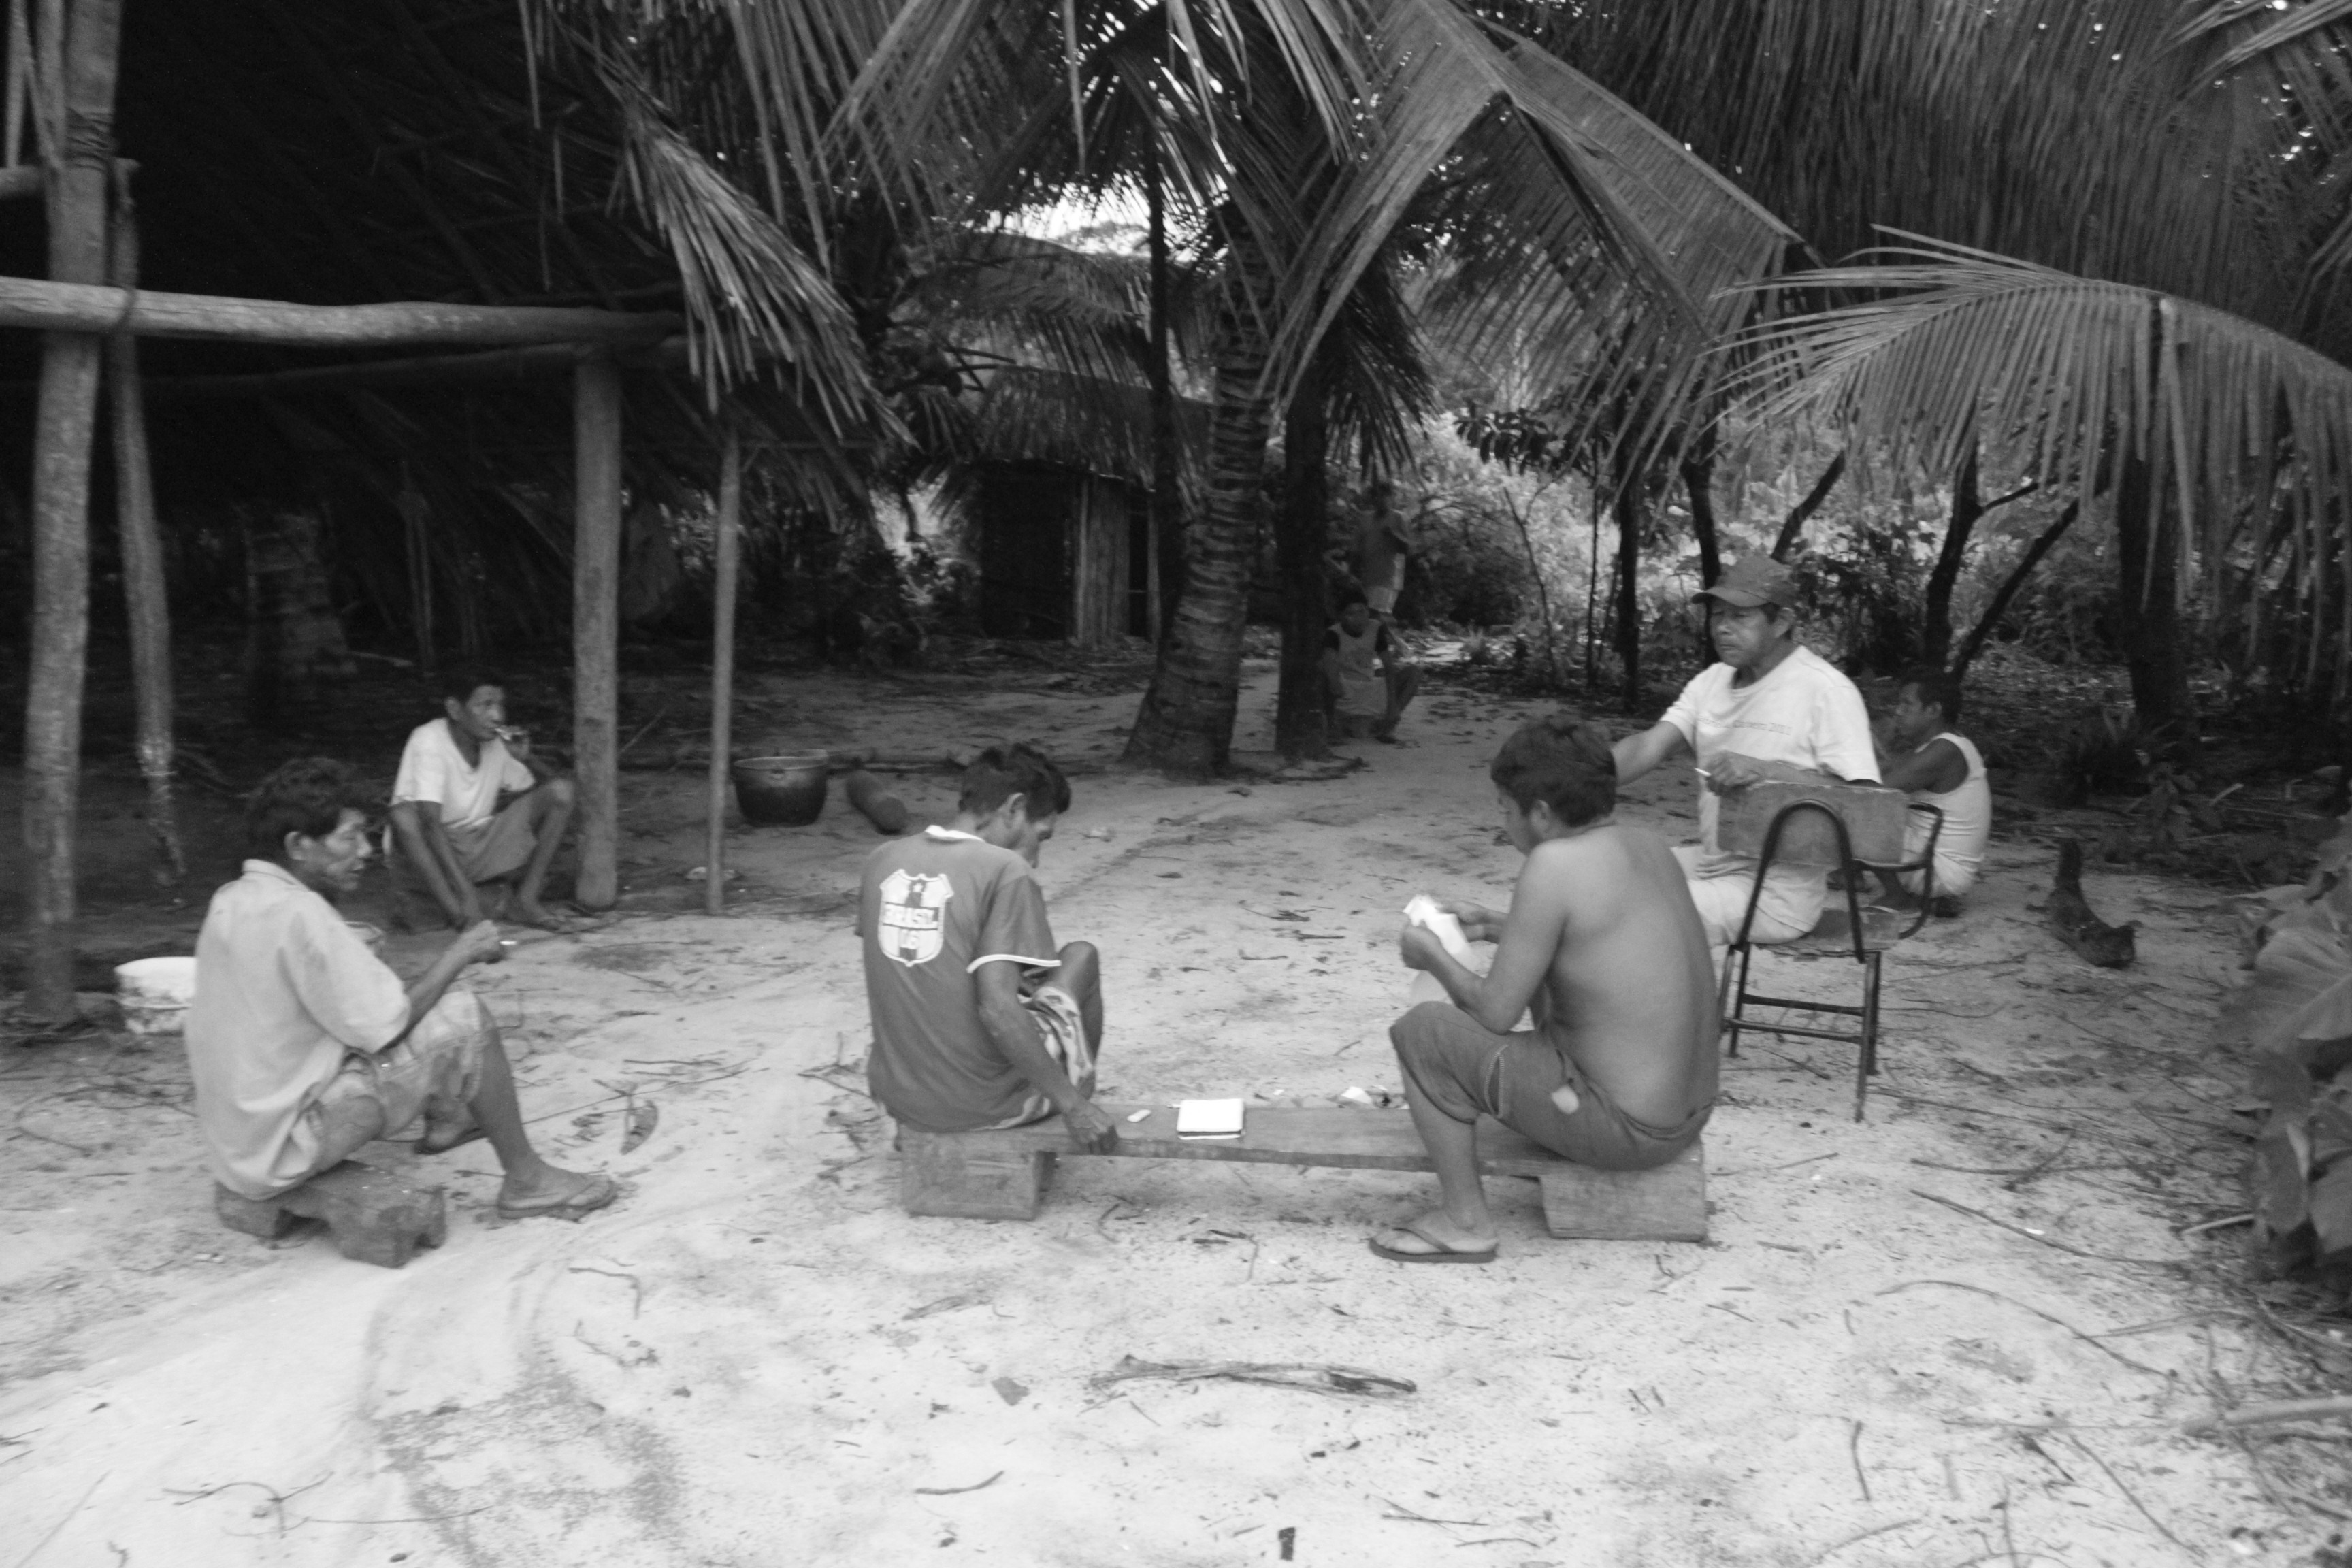
\includegraphics[width=\textwidth]{./img/032}
%\caption{Uma roda de coca (foto: Danilo P. Ramos, 2009)}
%\end{figure}

É dessa forma que se iniciam vagarosamente os encontros noturnos cujos
participantes são, em sua maioria, \textit{wähä̗d d'äh}, ``velhos hup'',
conhecedores das práticas xamânicas, das narrativas míticas e das
atividades de caça e pesca. Conversando animadamente e rindo uns dos
outros, todos vão procurando ``bancos hup'', \textit{hup kä̖d}, troncos caídos
ou, mesmo, espaços no chão para sentar"-se e esperar para comer a \textit{hib'a̗h
we̖d}, a ``comida do surgimento''. Vão assim se formando rodas que
estabelecem as linhas para a circulação da coca. Sentando"-se para \textit{pũ'ũ̖k
we̗d}, ``comer coca'', os senhores constituem os \textit{pũ'ũ̖k kökö̗t}, os
``círculos de coca''.

Em \textit{Ta̗t"-Dëh}, em muitas noites, rodas ocorrem simultaneamente. A mais
constante forma"-se em torno do pilão de Ponciano, herança de seu pai
falecido, Antônio. Uma segunda roda forma"-se próxima à casa do pajé
Firmino. Os participantes também se reúnem próximo às casas de Vicente e
de Luís. Os velhos alternam"-se entre uma roda e outra, dependendo do
dia, do convite e da quantidade de coca disponível. O número de
participantes pode ir de dois a dez. Em dias de festa de caxiri, até
vinte pessoas chegam a sentar"-se para comer coca e fumar.

À medida que vão se cumprimentando, cada um ocupa um lugar, geralmente
em frente ao pilão, à \textit{b'o̖'}, ``cuia'', e à \textit{mom"-b'o̗k}, ``panela de
metal''. Esses três objetos são manuseados para a produção e o consumo
da coca. Quando há muitos participantes, três deles começam a
preparação. Despejam na panela as folhas de coca colhidas por diferentes
pessoas. As folhas são remexidas com a mão para perderem a umidade dos
saquinhos plásticos. Depois, as folhas são esparramadas no ``forno'',
\textit{b'o̗k"-ka̗b}, previamente aquecido. Ao final da tarde, quando as mulheres
terminaram de torrar a farinha e/\,ou assar os beijus para alimentar a
família, os senhores hup começam a mexer as folhas para assá"-las ao
calor do forno.

Enquanto esperam o beiju ficar pronto, as mães sentam"-se com seus filhos
no colo ou entre as pernas, catam seus piolhos, entoam delicadas
melodias de ninar, conversam entre si sobre os acontecimentos do dia. É
uma hora de muita brincadeira. As crianças maiores correm em grupos de
casa em casa. As mulheres presentes sempre provocam os \textit{pũ'ũ̖k we̗d däh},
os ``comedores de coca''. Chamam"-nos pelos apelidos, debocham de suas
bocas verdes. Nesses momentos é comum que mães ou avós se aproximem de
um dos presentes, expliquem a doença que acomete algum de seus
familiares e lhe peça que realize um encantamento. Geralmente,
chegando"-se perto do benzedor que já está sentado, ela se agacha,
conversa com ele em voz baixa, entrega tabaco e papel, ou um copo com
líquido dentro e \textit{bi'i̖d ih kë̗y}, ``pede para benzer''. Em seguida, ela
se afasta da roda e senta"-se, mantendo certa distância dos participantes
enquanto o senhor executa o benzimento. De modo diferente, caso um
homem, jovem ou adulto, demande a ação xamânica, ele se sentará ao lado
dos participantes, partilhará o tabaco, mas não a coca.

Diz"-se que ocupa o ``primeiro banco'', \textit{kɨhsä̗t kä̖d}, aquele que se
encarrega de socar o pilão, misturar a coca com as cinzas de imbaúba e
filtrar o composto até derramá"-lo do pilão à cuia. Essa mistura será
oferecida aos demais presentes por um dos velhos ao seu lado e começará
a circular de mão em mão. \textit{O primeiro banco} foi a expressão usada por
Angélico para descrever o lugar que seu pai, Paulino ocupara nas rodas
quando começou a comer coca. Em 2009, o filho mais velho de Henrique,
Marino, ocupava constantemente o \textit{primeiro banco}. Tinha recebido o
\textit{benzimento da coca} para começar a comer diariamente o alimento. O
velho Firmiano o acompanhava e o instruía a cada encontro. Membro de um
clã afim aos \textit{Sokw'ä̗t"-Noh"-K'öd"-Tẽ̖h"-d'äh}, diz"-se \textit{brincando} que
Firmiano é o \textit{capitão coca}, o \textit{cozinheiro}. Cunhado, \textit{yo̖h}, de
Ponciano, Firmiano é o dono do \textit{primeiro banco} pelo qual devem passar
todos aqueles que começam a comer coca.

%\begin{figure}
%\centering
%\includegraphics[width=\textwidth]{./img/008}
%\caption{Instrumentos para preparo da coca (foto: Danilo P. Ramos, 2009)}
%\end{figure}

A riqueza gestual que compõe o preparo é impressionante. A coca é
colhida durante a tarde por um ou mais participantes em suas próprias
roças ou nas plantações de um ``dono da coca'', um \textit{pũ'ũ̖k yo'o̖m ĩh}.
Enquanto as mulheres trabalham com a mandioca, os senhores vão até os
pés de coca e começam a colher as folhas, cuidadosamente retiradas uma a
uma. Diante dos pés de coca, o senhor abaixa seu corpo e realiza a
colheita de cócoras, retirando delicadamente as folhas com as duas mãos
e olhando atentamente a planta. Evita"-se deixar o pé de coca
inteiramente sem folhas. No meio do caminho rumo à roça, apanha"-se uma
folha verde de imbaúba para que as folhas de coca colhidas possam ser
depositadas nela, caso não haja sacola plástica. Quando já há uma boa
quantidade de coca, fecha"-se a folha de imbaúba e amarra"-se com um cipó
fino. A trouxinha pode ser carregada numa das mãos ou em volta do
pescoço como uma mochila pequena. Como nas descrições de C. Hugh"-Jones
(1979) e S. Hugh"-Jones (1979), chama a atenção o paralelo entre a
atividade feminina da roça de mandioca e a atividade masculina de
velhos, da colheita de coca. Terminada a colheita, o \textit{comedor de coca}
volta para a aldeia e pendura a trouxa com folhas nas palhas do telhado
da cozinha coletiva, perto dos instrumentos de produção da coca.

Certo dia, Ponciano veio visitar"-me na hora do almoço. Comemos juntos.
Arroz, lentilha e banana. Rimos muito com as duas bananas grudadas
(gêmeas), pois ele disse que apenas os mais velhos podiam comer bananas
assim. Para os mais jovens, comê"-las representa perigo. Ele estava a
caminho da roça e disse que eu poderia acompanhá"-lo. Apanharíamos
\textit{pũ'ũ̖k}. Saímos da aldeia por um caminho que se abre a oeste em direção
à roça de Vicente, seu irmão. Sempre no mesmo passo ritmado, Ponciano
seguia à frente e guiava"-me nos momentos mais difíceis. Em lugares de
terra úmida e igarapés pequenos, ele procurava sempre andar sobre as
raízes das árvores. Fomos passando pelas roças de outras pessoas, todas
cheias de maniva. Crianças brincavam às margens do caminho num dos
trechos. Meia hora depois, chegamos à roça de Vicente. No percurso,
atravessamos uma ponte feita com um tronco e duas varas de apoio. Depois
disso, troncos de árvore grandes transformavam"-se em caminhos. Era
perigoso andar no chão, pois podia haver cobras. Íamos como
equilibristas sobre esse caminho de toras, vendo de cima as plantações
que se espalhavam a nossos pés.

Uma mulher e uma jovem trabalhavam na plantação de mandioca naquelas
roças. A jovem parou seu trabalho para ajudar"-nos na colheita. De
cócoras, Ponciano mostrou"-me como fazer para colher a coca. Apoiava o
dedão na haste (pecíolo) da folha. A outra mão retirava a folha
cuidadosamente. Os punhados eram colocados numa folha verde de imbaúba.
A sobrinha de Ponciano ajudou"-nos até enchermos a imbaúba. No final, o
cipó que envolve a folha foi fechado com o monte de coca dentro.
Ponciano colocou a trouxinha em torno do pescoço e seguimos de volta
para a comunidade. Ao chegarmos, a trouxinha com coca foi pendurada numa
das ripas do telhado da cozinha. Eu deveria me dirigir ao igarapé para
banhar"-me, enquanto Ponciano buscaria folhas de imbaúba seca nos
arredores da aldeia.

Já no final de minha última viagem de campo, fui com Américo à sua roça
colher coca. Ele contou que uma mão de coca é chamada de \textit{kimi̖t}. Dez
\textit{kimi̖t} são considerados uma grande quantidade de coca. A medida permite
o controle do montante de coca que será retirado e levado para a
preparação. Há duas formas de plantar a coca. Uma delas é dispor os
``ramos de coca'', \textit{pũ'ũ̖k"-tig}, em círculo. O nome desse arranjo é \textit{sih
kökö̗t}, traduzido por Américo como sendo o modo ``rodado'', ``em
círculo''. Essa é a maneira como os antigos a plantavam para que os pés
de coca conversassem entre si como os senhores conversam nas rodas
noturnas, também chamadas de \textit{pũ'ũ̖k kökö̗t} pelos antigos, ``círculos de
coca''. Atualmente, planta"-se como os Tukano, em fila. Também nesse
arranjo os pés conversam entre si. O nome desse modo de plantação é
\textit{pũ'ũ̖k ka̗'}. A coca deve ser plantada na ``terra firme'', \textit{m'aj' kɨ̗'}.
Esse tipo de solo, considerado muito fértil, surgiu quando um ancestral
com o mesmo nome entrou na terra.

Ao longo da pesquisa de campo, todas as noites em que eu participava dos
encontros noturnos, perguntava qual tipo de coca estávamos comendo. O
\textit{pũ'ũ̖k"-s'a̗}, ``coca preta'' é o gênero mais consumido. Está também
presente nas roças de pelo menos onze dos participantes das rodas. Essa
coca de folhas médias é considerada ``um pouco doce'', \textit{si̗m'eh k'ä̗h}. O
tamanho da folha e o grau de doçura são os principais critérios de
classificação utilizados para diferenciar as plantas. Em dias de festa
de caxiri, comíamos o \textit{wahna̗w"-pũ'ũ̖k}, a ``coca de abiu'', que possui
folhas pequenas. Esse é considerado o tipo mais doce de coca. Todos os
participantes das rodas possuem pelo menos alguns pés dessa coca em suas
roças. Essa é também a ``coca da origem'', \textit{hib'a̗h"-pũ'ũ̖k}, aquela que
foi dada por \textit{K'e̖g"-Tẽh} à humanidade. Como visto no capítulo anterior,
essa coca é também encontrada à beira do lago de banhar, no alto da
Serra Grande. Outros tipos de coca são: a ``coca árvore'',
\textit{tëg"-d'u̗h"-pũ'ũ̖k}, pouco doce e de folhas pequenas; a ``coca piaba'',
\textit{hu̗y"-pũ'ũ̖k}, pouco doce e de folhas pequenas; a ``coca anta'',
\textit{ta̖h"-pũ'ũ̖k}, igualmente pouco doce e de folhas grandes; e a ``coca
sapo"-cururu'', \textit{hoho̗h"-pũ'ũ̖k}, de folhas pequenas e pouco doce.

\begin{table}%[]
\centering
\resizebox{\textwidth}{!}{%
\begin{tabular}{@{}lllll@{}}
%\toprule
\textbf{Nome} & \textbf{Tradução} & \textbf{Folha} & \textbf{Sabor} & \textbf{Potência} \\ \midrule
\textit{Wahna̗w"-pũ'ũ̖k} & Coca abiu & Pequena & Muito doce & Muito forte\\
\textit{Pũ'ũ̖k"-s'a̗} & Coca preta & Média & Pouco doce & Forte\\
\textit{Tëg"-d'u̗h"-pũ'ũ̖k} & Coca árvore & Pequena & Pouco doce & Forte\\
\textit{Hu̗y"-pũ'ũ̖k} & Coca piaba & Pequena & Pouco doce & Forte\\
\textit{Ta̖h"-pũ'ũ̖k} & Coca anta & Grande & Pouco doce & Forte\\
\textit{Hoho̗h"-pũ'ũ̖k} & Coca sapo cururu & Pequena & Pouco doce & Forte\\
\bottomrule
\end{tabular}
}
\caption{Tipos de coca e características principais.}
\label{q1}
\end{table}

Durante o encontro, folhas de caderno e saquinhos com tabaco
industrializado vão sendo tirados dos bolsos e passam de mão em mão.
Cada um prepara seu ``cigarro'', \textit{hũ̖t sop}, coloca"-o na boca e acende"-o
com fósforos, isqueiros ou com o fogo sob o tacho que aquece as folhas
de coca. Contam que antigamente todos os velhos tinham grandes
plantações de tabaco, mas que, com o tempo, essas plantações foram
acabando. Possuíam um método de produção do tabaco para o fumo
semelhante ao do fumo de corda, mas armazenavam"-no na forma de bolas
secas, \textit{hũ̖t pan'}, guardadas em sacos de folha de bananeira. O \textit{hũ̖t},
``tabaco'', é dito ser o ``irmão da coca'', o \textit{pũ'ũ̖k ba̗b'}. Certa noite,
Samuel, filho de Ponciano, disse: \textit{hũ̖t pã̖, pũ'ũ̖k na̗g nɨ̗h, hũ̖t pũ'ũ̖k
k'o̗y, hũ̖t pũ'ũ̖k ba̗b'}, ``se não há tabaco, a coca não tem óleo, o tabaco
acompanha a coca, o tabaco é o irmão da coca''.

Em 2012, somente Manoel afirmava ter ainda sementes de tabaco e alguns
poucos pés plantados em sua roça. Apenas em dias de festa ele preparva
cigarros com esse tabaco, cujas sementes e mudas recebera de seu pai,
Francisco. Levando em consideração a dificuldade de se obter tabaco para
o consumo nos encontros noturnos e o fato de comerem coca diariamente,
propus aos participantes que ofertaria à roda um maço de fumo por noite
como forma de troca. Junto com meu caderno de notas, levava sempre um
pacote de tabaco e folhas de papel almaço para que os presentes pudessem
preparar seus cigarros e \textit{temperar} a coca. A troca sempre foi
apreciada por todos e diziam sentir falta de minha oferta quando eu
estava longe.

O fogo vai assando as folhas de coca que se tornam secas e duras. É
preciso estar diante do tacho todo o tempo juntando as folhas com as
mãos e jogando"-as para o alto para que fiquem assadas por igual. O olhar
e a concentração fixam"-se na coca, havendo pouca conversa com os outros
participantes. Enquanto isso, uma terceira pessoa recolhe as grandes
folhas secas de imbaúba (família das cecropiáceas, \emph{Cecropia sp.}),
em língua hup chamadas \textit{pũ'ũ̖k b'ö̖h}, ``sal de coca''. A imbaúba cresce
nas capoeiras e é recolhida no entorno da aldeia. Apesar de predominar o
uso da imbaúba, as folhas da ``imbaúba roxa'' (família das cecropiáceas,
\emph{Cecropia purpurascens}), \textit{b'ab'a̖'}, do ``açaí'' (palmeira da
família das arecáceas, \emph{Euterpe sp}.), \textit{ker'a̗g}, e da ``pupunha''
(palmeira da família das arecáceas, \emph{Bactris gasipaes}), \textit{sɨ̖w
k'e̖t}, também podem ser utilizadas como \textit{sal de coca}. Próximo à roda,
as folhas são amontoadas sobre uma chapa de latão e queimadas. As chamas
intensas transformam pouco a pouco as folhas em cinzas. A fumaça negra
espalha"-se pelo ar próximo à roda e pode ser vista mesmo de longe por
todos da aldeia. É também um sinal de que o encontro noturno está
começando. As cinzas de imbaúba são peneiradas no \textit{pũ'ũ̖k b'ö̖h sɨ̗m'},
tipo de balaio usado para reduzir as cinzas a pó.

Depois de assadas, as folhas de coca são colocadas no pilão da coca e
socadas até ficarem totalmente trituradas, já constituindo em parte um
fino pó verde. O preparador fica em pé, os olhos fixos no pilão. Mantém
seu corpo erguido e realiza movimentos precisos com o socador.
Arremessa"-o para baixo contra o fundo e puxa"-o para cima para um novo
soco. Quando o pó já começa a sair pela boca do pilão, e uma fumaça
verde envolve o corpo do preparador, é sinal de que a coca pode ser
derramada na cuia. O preparador retira o pau, traz a cuia para perto de
seus pés, ergue e vira o tubo, deixando a coca escorrer para a cuia.
Nesse momento, parte da coca já constitui o pó, mas restam ainda
pequenos pedaços.

As cinzas das folhas de imbaúba são misturadas à coca na panela e depois
a solução é despejada num pano. Fecha"-se o pano na forma de ``saco'',
\textit{pũ'ũ̖k"-pɨ̖h}, com um cipó que o amarra à ponta de um pau mais fino e
menor que o do pilão. O preparador senta"-se em seu banco, coloca o saco
dentro de uma panela, cobre"-a com outro pano para impedir a saída do pó
e começa a fazer movimentos pendulares e rápidos com o pau, ao mesmo
tempo em que soca levemente o fundo da panela. Esse procedimento pode
durar até 15 minutos, e é através dele que o pó a ser consumido começa a
surgir no fundo da panela após a filtragem. O composto em pó é então
derramado na cuia e entregue aos velhos que estão ao lado do preparador.

O que resta no pano é colocado novamente no pilão e retriturado. Esse
procedimento repete"-se até que a maior parte da mistura de coca com
imbaúba tenha se transformado em pó. Entre uma pilagem e outra, pequenas
porções são retiradas para que alguns participantes \textit{we̖d kë̗y},
``experimentem'', a comida e digam se o \textit{tempero} está bom. Muitas
vezes, ao explicar"-me o modo de preparo, os senhores diziam que é
preciso experimentar para ver se foi colocada a quantidade suficiente de
cinzas de imbaúba, ou, como diziam, \textit{tem que ver se está bom de sal}.
A mistura deve deixar a coca menos doce, pois há uma relação entre o
grau de doçura e a força do alimento. Quanto mais doce, mais forte a
coca. Consumir a coca sem o \textit{sal} ou com uma quantidade insuficiente
faz com que a pessoa não consiga dormir durante a noite e, no dia
seguinte, não saia da rede para trabalhar.

A técnica utilizada para lançar a coca na boca é muito importante.
Atualmente os participantes utilizam uma colherinha para jogar o pó nos
dois cantos da boca ou sob a língua. Antigamente, os antigos usavam um
``osso de jacamin'',\footnote{Jacamim, ave da família dos psofídeos,
  \emph{Psophia crepitans}. Cf. Ramirez (2006).} \textit{meme̗ç k'e̖g}, para
``chupar'', \textit{o̗no̗y}, a coca. Segundo Ponciano, era muito perigoso, pois
ao chupar o osso o pó podia ir para a garganta. Caso o pó seja lançado
diretamente na cavidade bucal, ele se espalha indo para a cavidade
nasal, laringe e traqueia, causando tosses, engasgos e lágrimas.
Possivelmente também leve ao riso dos outros, como aconteceu comigo nas
primeiras vezes em que participei da roda. O certo é deixar o pó nos
cantos da boca ou sob a língua e ir absorvendo"-o vagarosamente.
Misturada à saliva, a coca transforma"-se numa pasta que vai aos poucos
sendo digerida. Os cantos da boca na parte externa ficam verdes e, à
medida que absorvem a coca, os senhores continuam conversando e fumando.
Isso faz com que uma fumaça verde se forme diante de suas faces,
iluminadas pela brasa dos cigarros. Quando já não há mais coca para
reabastecer a cuia, inicia"-se novamente o processo de produção para que
haja outra \textit{rodada}, como dizia Jovino. Os participantes dizem que a
``coca vai'', \textit{pũ'ũ̖k ha̗ma̗y}, quando se referem ao movimento de
circulação da cuia.

Durante uma roda, Ponciano comentou que os ancestrais não usavam latas
nem potes de plástico para fazerem a coca circular. Usavam os antigos
\textit{m̗j wõwõ̗y'}, ``potes'', feitos com cipó e vedados com breu. Eram usados
para guardar a coca e o tabaco e para oferecê"-los aos participantes dos
encontros. A partir do desenho desses potes antigos foi feito na areia
por Angélico como ilustração numa outra roda.

%\begin{figure}
%\centering
%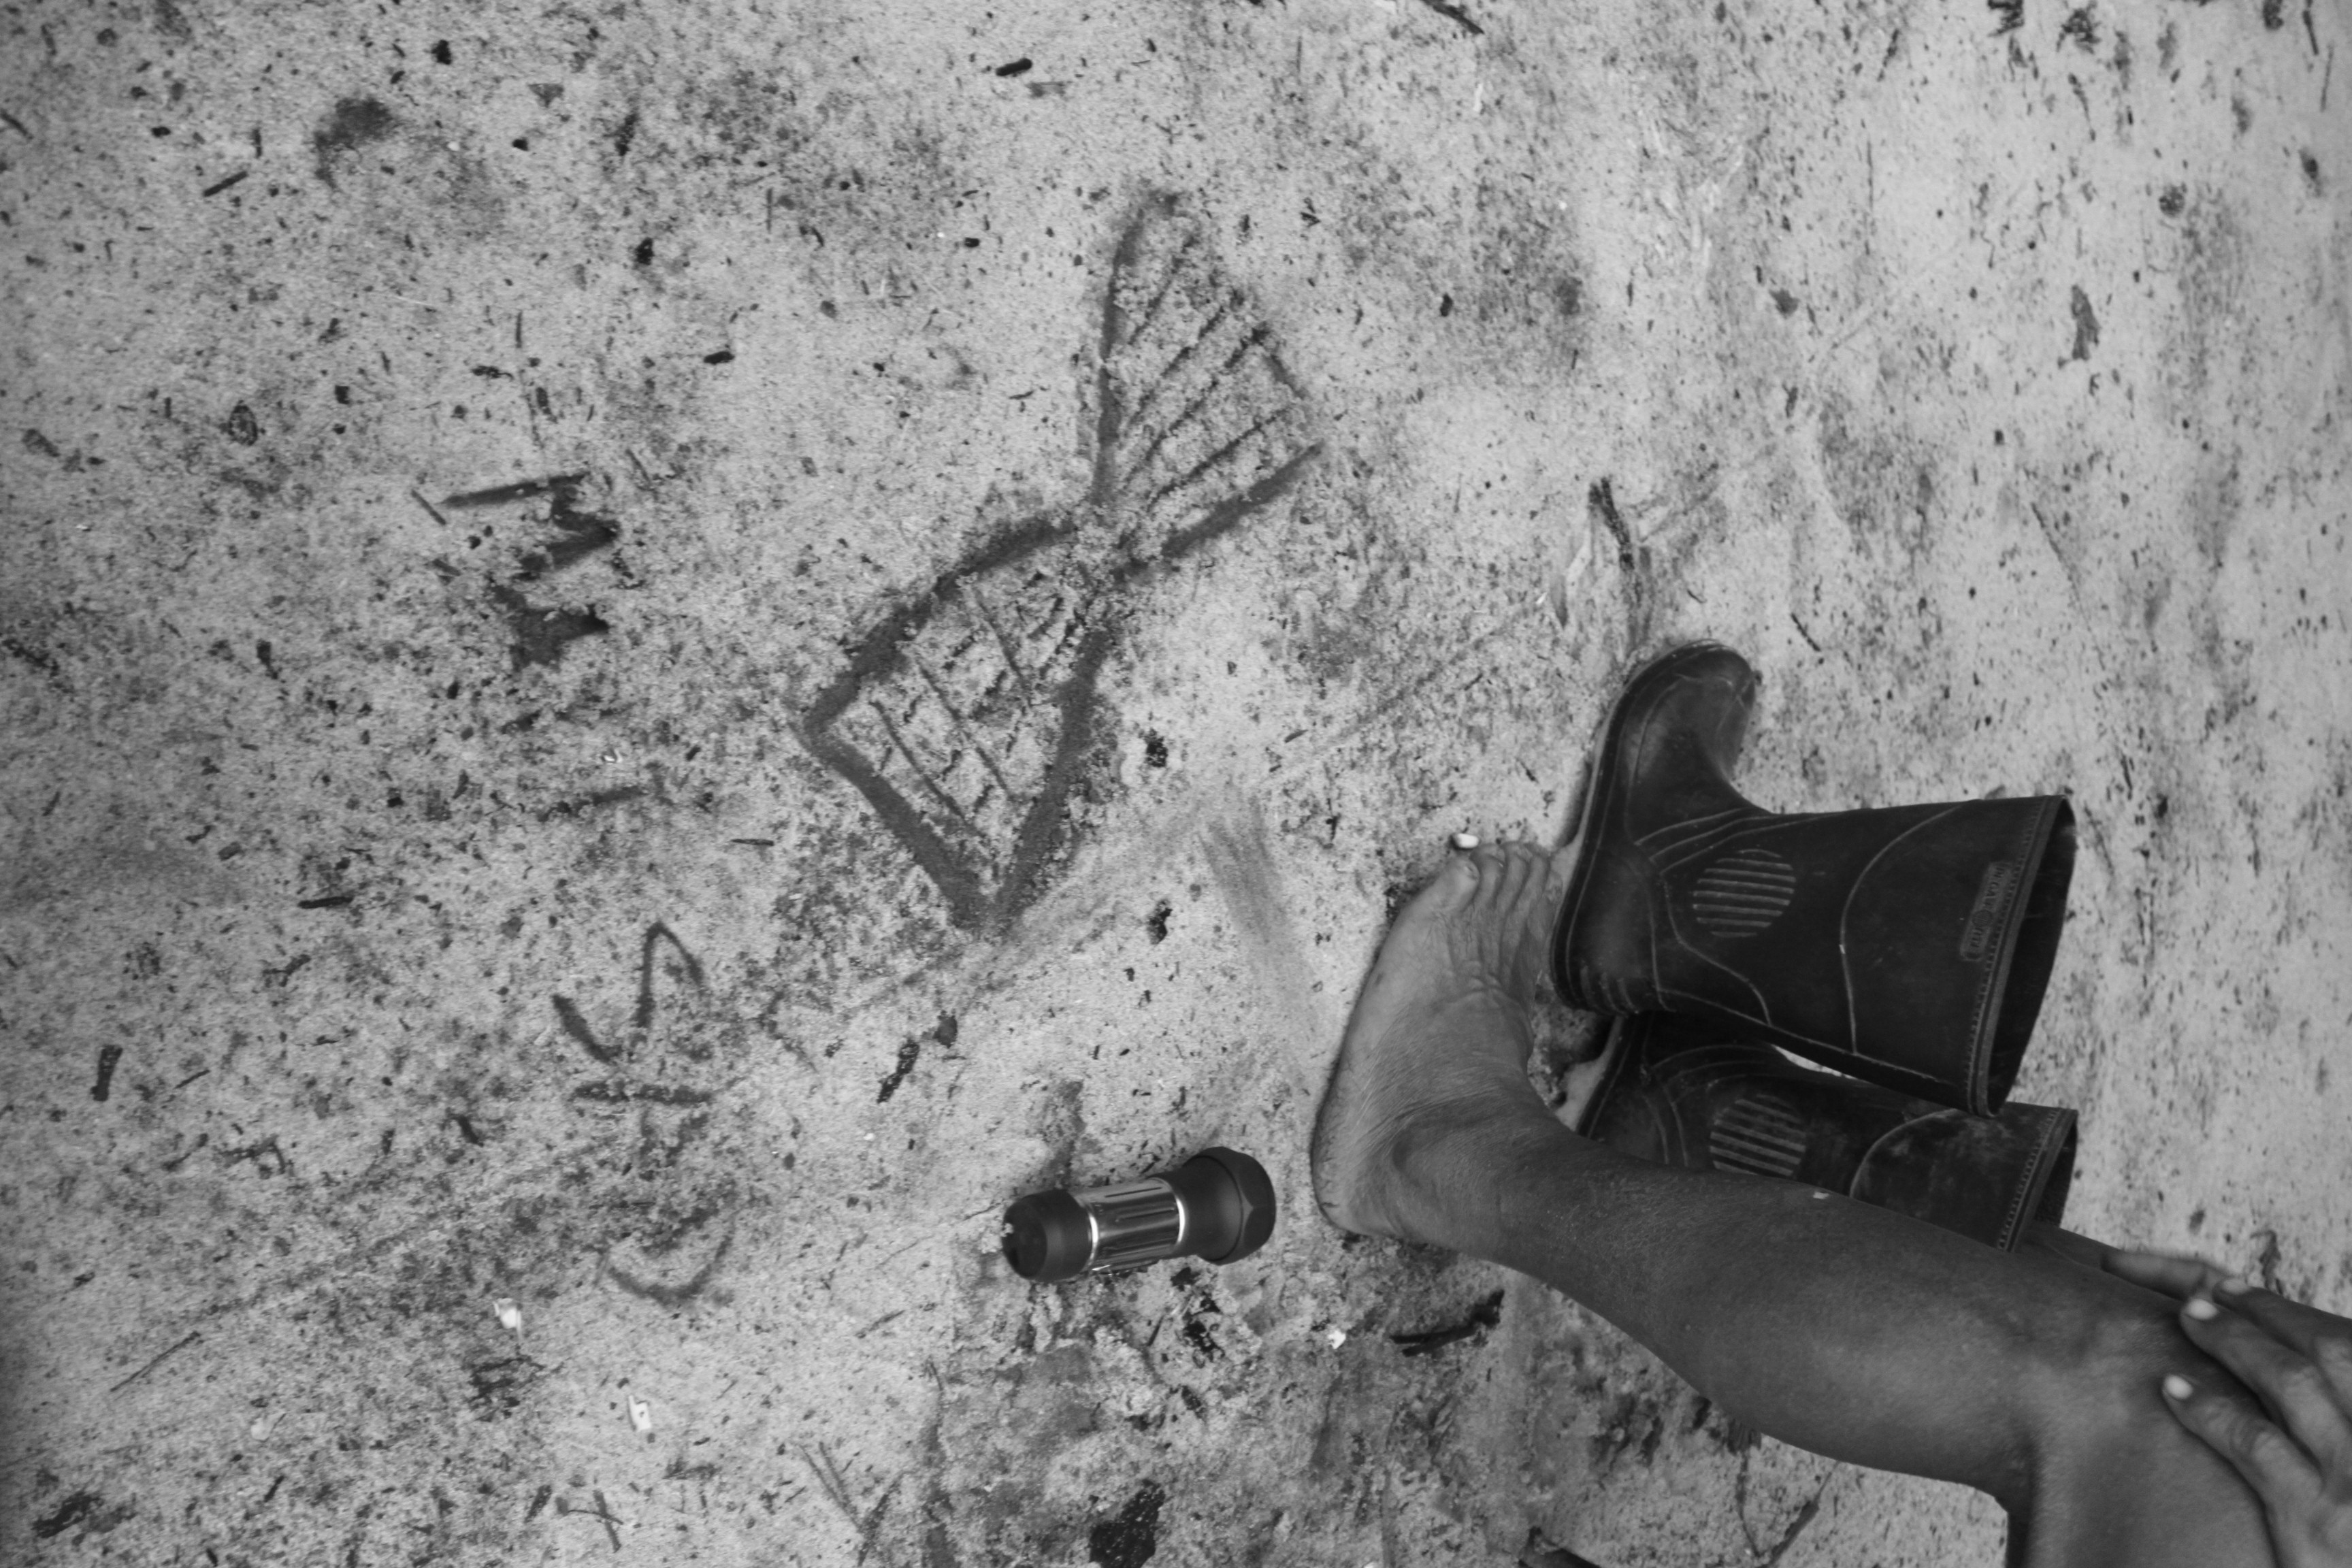
\includegraphics[width=\textwidth,angle=90]{img/009}
%\caption{Antigo pote de coca e tabaco}
%\end{figure}

Um homem só começa a participar dos encontros noturnos quando já tem
filhos ``jovens'', \textit{pesa̖w}. São geralmente considerados \textit{wähä̗d'däh},
``velhos''. Com a escuridão da noite e o silêncio da aldeia, os
presentes começam a preparar a coca e a comunicar"-se a partir de modos
de fala específicos. Durante a preparação, os presentes chamam"-se por
apelidos, riem uns dos outros, provocam as mulheres próximas. Os
sucessos na pesca ou na caça, a chegada de brancos, as viagens a São
Gabriel são temas frequentes nesses primeiros momentos em que os homens,
ainda que sentados, movimentam"-se bastante e levantam"-se de tempos em
tempos para ajudar os outros na preparação. Conforme o alimento começa a
ficar pronto, aqueles que ainda não se banharam dirigem"-se até o igarapé
para esfriar e limpar o corpo.

À medida que o espaço próximo à roda vai esvaziando"-se, o barulho
diminui, e ``histórias sobre os antigos'', \textit{pɨnɨ̖g}, são contadas e
discutidas, assim como ``encantamentos'', \textit{bi'i̖d}. Os apelidos dão lugar
ao termo de parentesco \textit{sät}, ``irmão maior'', usado como pronome de
tratamento, o que produz um sentido respeitoso, de modo semelhante ao
uso do pronome \textit{senhor} em português. Entre afins ocorre também a
alternância dos termos \textit{yo̖h}, ``cunhado'', \textit{semú}, do nheengatu
``cunhado'', e \textit{cumpa̗}, do português ``compadre''. O desempenho de
benzedores ausentes é motivo de avaliações e críticas. Juntos, os
participantes debatem também as causas de doenças que afligem a
comunidade e as melhores formas de proteger e curar. Os sonhos relatados
por seus parentes próximos ao longo do dia são interpretados e remetidos
a mitos e a benzimentos.

Ao cabo de três a cinco \textit{rodadas} termina o estoque de coca colhido
para o encontro noturno. Os preparadores comunicam ao grupo o término
dizendo: \textit{we̖d toho̗ yɨ̗'ɨ̗h}, ou \textit{pũ'ũ̖k toho̗ yɨ̗'ɨ̗h}, ``acabou a comida'' ou
``acabou a coca''. Os senhores começam a se despedir, levantar"-se
lentamente de seus lugares e retornar para suas casas. Restando ainda um
pouco de pó de coca, insuficiente para uma \textit{rodada}, esse é dividido e
armazenado nos ``potes de plástico ou latas'', \textit{pũ'ũ̖k tö̗d'}, e entregues
aos ``donos da coca'', \textit{pũ'ũ̖k yo'o̖m ĩh}, que a consomem ao longo do dia
seguinte, ou guardam"-na para oferecer no próximo encontro.

\section{\textit{Pũ'ũ̖k}, «coca»}\label{puuk-coca}

%\paragrahph{osso de coca}\label{osso-de-coca}

O fogo ia assando a carne do \textit{M'e̖h hup ĩh}, o Velho Cobra. No tacho
de ferro seus pedaços iam sendo mexidos pelos preparadores. De tempos em
tempos, recolhiam um pedaço e experimentavam sua textura para ver se a
carne estava no ponto. Muitos já haviam chegado para o encontro noturno.
Sentados em bancos, em pedaços de tronco ou no chão, conversavam
animadamente. Os preparadores recolheram a carne e colocaram"-na toda
dentro de um pilão. Em pé, um senhor hup ia golpeando o fundo do pilão
com força e precisão. O tronco oco mastigava os restos mortais a cada
soco. O som dos ossos despedaçando"-se contra a madeira ecoava por toda a
aldeia. Quando um pó verde começou a ser cuspido pela boca do pilão, o
preparador derramou o conteúdo em uma cuia. O outro preparador trazia o
sal para temperar a carne assada do Velho Cobra. Depois de salgada,
a carne e os ossos triturados foram peneirados e o fino pó despejado num
pequeno pote.

Um dos donos veio recebê"-lo para oferecer a todos, entre irmãos e
cunhados, que estavam sentados conversando. O pote circulava de mão em
mão. Cada um jogava o pó dentro da boca e passava o alimento para o
seguinte. Os cigarros iam sendo enrolados para acompanhar a refeição,
pois são eles que molham, com seu óleo, a carne e os ossos do Velho
Cobra. Toda a refeição era feita a partir de seu dedo menor, arrancado
por sua filha mais velha, \textit{Hõp Hup ã̗y}, a Mulher Peixe. Ela roubara
seu dedo sem que ele percebesse para entregar a seu marido \textit{Wed B'ö̖'}.
Foi ele quem fez a coca germinar para os Hupd'äh.

Descrevendo a roda de coca dessa maneira em meu caderno de campo, tomava
como referência os comentários de Samuel durante o encontro noturno em
que ele explicitou as relações entre a \textit{história de \emph{Wed B'ö̖'}} e o
modo como a cada noite as ações eram atualizadas. Em suas palavras,

\begin{quote}
O som do pilão que ouvimos é o osso da coca. A folha assando no forno é
a carne do Velho Cobra. A coca é o dedo dele. A imbaúba misturada é
o sal, tempero para a carne assada. O tabaco é o irmão da coca. Sem
tabaco a carne não tem óleo.\footnote{Caderno de campo, 8 de julho de 2012.}
\end{quote}

Observando a roda há mais de um ano e tendo ouvido a \textit{história de \emph{Wed
B'ö̖'}}, contada pelo pai de Samuel num encontro noturno em agosto de
2011, ainda não tinha percebido a analogia entre esses encontros e essa
história de \textit{Wed B'ö̖'}.

\begin{quote}\index{18@\textsc{m}9\quad História de \textit{Wed B'ö̖'}}
\mito{9}{história de \textit{wed b'ö̖'}}

Tinha um homem, aquele \textit{Wed B'ö̖'}. Perto de sua casa havia uma árvore
que dava uma frutinha como miçanga. Duas moças, filhas do \textit{M'e̖h hup}, o
Velho Cobra, iam lá para tirar a fruta e comer. O homem foi lá e
esperou"-as com sua zarabatana, cujas setas estavam envenenadas. Acertou
a moça, que caiu. Ele tentou benzê"-la para que ela voltasse, mas não
conseguiu.

Então ele cavou um buraco e enterrou"-a. Foram esses bichinhos que cavam
buraco na terra, esses que aparecem agora em agosto, que a fizeram
reviver. Ele a desenterrou e a levou para casa. Tentou dar"-lhe vários
tipos de comida, mas ela não comia.

Depois, quando ela tecia uma pulseira de tucum para o marido usar na
canela, uns passarinhos vieram e foram levando o fio de tucum. Eram as
irmãs dela que queriam saber como ela estava. Ela disse para o marido
que precisava ir para a casa do pai, mas o marido não queria deixar.
Quando acabou de casar, o marido não deixa a esposa. Só quer ficar
junto. A Mulher Peixe caiu na água e foi para a casa do pai.

Lá ela começou a pegar beiju, farinha, moqueados, tudo. Foi e pegou um
galho de coca, mas diz que a coca é o osso do \textit{M'e̖h Hup}, o Velho
Cobra. O pai sentiu aquela dor no dedo e pensou: \textit{Será que minha
filha está me roubando?}. Foi e olhou todo o corpo dela. Só não olhou a
vagina, pois se diz que é ruim o pai da moça olhar a vagina dela. Lá ela
tinha escondido o galho de coca.

Quando chegou na data marcada, ela foi dando comidas para o marido. Mas
ele desmaiava com cada alimento que punha na boca. Comeu moqueado e
desmaiou, ao beber caxiri desmaiou também. É aí que começa o benzimento
do caxiri. O marido dormiu e, quando acordou no dia seguinte, havia um
pé de coca plantado. Não precisava tirar as folhas. Era só balançar o pé
e colocar a cuia embaixo e já enchia de coca. O mesmo acontecia com o pé
de tabaco que também estava plantado. Todos os tipos de coca surgiram
aí, o \textit{pũ'ũ̖k"-s'a̖}, a ``coca preta'', o \textit{wahna̗w"-pũ'ũ̖k}, ``coca abiu'', e
os diferentes tipos de tabaco.
\end{quote}

Essa era a segunda vez que Ponciano contava a história de \textit{Wed B'ö̖'}
para mim. A primeira tinha sido quando comecei a fazer a gravação das
narrativas e benzimentos na roda. Eu ainda trabalhava a tradução escrita
da história com seu filho mais novo, Sabino. Para que eu entendesse o
conteúdo da história, ele a contou novamente para que seu filho mais
velho, Jovino, a traduzisse aos poucos para mim. Ponciano revelou"-me que
muitos encantamentos como o da coca, do tabaco, do caxiri e da roça têm
origem nessa história. O narrador contava e perguntava aos outros
participantes da roda se estava certo o que dizia: \textit{Yid}, ``É isso?'',
ao que os outros confirmavam dizendo: \textit{Yid}, ``sim''. Por vezes,
acrescentavam fatos e corrigiam o narrador. Jovino ouvia atentamente a
fala do pai e, de tempos em tempos, começava a traduzir em português.
Minha fluência na língua ainda não me permitia ouvir e entender bem as
\textit{pɨnɨ̖g}, ``histórias''.

Nas ações dos ``ancestrais'', \textit{hib'a̗h tẽ̖h d'äh}, encontram"-se os
acontecimentos que fazem aparecer malefícios que afligem os Hupd'äh até
hoje. Ao mesmo tempo, surgem os encantamentos que ajudam a curá"-los.
Numa roda de coca dias antes, Ponciano contou que a coca tem uma
essência ruim. Isso se deve ao fato de a Mulher Peixe ter colocado o
galho, o dedo, o ramo de seu pai, na vagina. A cera de sua vagina
impregnou"-se na coca. Essa cera faz mal e deve ser tirada. É nesse ponto
da história que surge o \textit{benzimento da coca} e também os malefícios,
como o sono durante o dia, a impotência sexual e o enfraquecimento do
corpo. A partir do ato de \textit{Wed B'ö̖'} de beber e desmaiar, surgem o
malefício de \textit{äg na̗'ap i,h}, ``morrer de beber'' ou ``desmaiar de
bêbado'' e o ``benzimento do caxiri''. Enquanto traduzia a história,
Jovino localizava o momento preciso em que surgiu esse malefício para
indicar o momento do aparecimento do encantamento.

\index{18@\textsc{m}9\quad História de \textit{Wed B'ö̖'}}
Em \textsc{m9}, duas perspectivas, dois modos de percepção parecem estar
em jogo. Num primeiro momento, o ancestral hup ocupa a posição
predominante, mata a Mulher Peixe com sua zarabatana e depois a acolhe.
Tenta alimentá"-la, mas ela se recusa a comer o que lhe é oferecido.
Depois, a esposa viaja para visitar os pais e retorna para alimentar o
marido. Ela realiza uma mediação entre as duas perspectivas
concorrentes, a das Gentes"-Cobra, da qual faz parte, e a das Gentes"-Hup,
com as quais estabelece aliança através do casamento. O osso da coca
revela a imagem que justapõe essas duas perspectivas, já que \textit{a coca
dos Hupd'äh é osso de Gente"-Cobra}.

Nas rodas de coca, talvez o primeiro malefício a ser atenuado ou
revertido seja a ação da Mulher Peixe de arrancar o dedo do pai e
escondê"-lo na vagina. Assar a coca ou a carne, pilar os ossos são processos
que provavelmente revertam a agência destrutiva da coca enquanto carne
de Gente"-Cobra e a tornem um alimento limpo, bom para o consumo e para a
conversa. Tudo ocorre como uma predação onde os senhores hup procuram
assumir o ponto de vista dominante nessa relação com as
Gentes"-Cobra. Isso se dá através de suas agências mítica e xamânica.
Entendo que a partilha da carne e da coca e a comensalidade produzem relações
entre parentes.\footnote{Nas palavras de Fausto (2002, p.\,15), ``A
  partilha da carne e a comensalidade não apenas marcam as relações
  entre parentes, como as produzem. Comer como alguém e comer com alguém
  é um forte vetor de identidade, assim como se abster por ou com alguém.
  A partilha do alimento e do código culinário fabrica, portanto,
  pessoas da mesma espécie''.}

Nas rodas, ao preparar a coca, todos sabem que preparam a carne e o osso
do Velho Cobra. Comendo com os parentes hup, os participantes comem
também como o ancestral que estabeleceu um laço de comensalidade e de
casamento, ao mesmo tempo em que predava o sogro.

Aproximando"-me da reflexão de Gow, considero que os encontros noturnos,
nas ações de preparação da coca, constituem gestualmente um \textit{agora}
estabelecido pelo ato de os participantes voltarem sua atenção
mutuamente para eventos, movimentos e seres buscando situar"-se entre as
perspectivas. Se em \textsc{m9} o \textit{roubo do dedo} é condição para que
a coca, o tabaco e os benzimentos \textit{apareçam} para os Hupd'äh, a
transformação do \textit{osso da coca} em todas as noites permite que
diariamente esses alimentos, os encantamentos e as histórias
\textit{apareçam} para os participantes.
\index{18@\textsc{m}9\quad História de \textit{Wed B'ö̖'}}

\section{A essência ruim da
coca}\label{a-essuxeancia-ruim-da-coca}
% Please add the following required packages to your document preamble:
% \usepackage{longtable}
% Note: It may be necessary to compile the document several times to get a multi-page table to line up properly



\begin{comment}
\begin{longtable}[c]{lllll}
\label{b1}\\
\multicolumn{4}{l}{\textbf{B1 - /Pũ'ũ̖k bi'i̖d/ ‒ Benzimento da coca}} \\
\endfirsthead
%
\endhead
%
&  &  &  \\
1º mov &  &  & \begin{tabular}[c]{@{}l@{}}Eu vou contar para você, Danilo. Eu faço a casca \\ de abiu, a casca de tururi transformarem-se na \\ água-pura que há dentro (dessas árvores). \\ Transformo a água-pura  de dentro do ramo \\ de coca de onde vem a /hã̗wag-dëh/, a ``água do \\ sopro vital''.\end{tabular} \\
 &  &  & \begin{tabular}[c]{@{}l@{}}\emph{(Com.)} Menciono as águas-puras dali para extrair \\ sua essência ruim, a ``pasta da coca'', /pu͂'u̖͂k nu̖h/. \\ Essa impureza pode causar doenças como o sono \\ de dia.\end{tabular} \\
 &  &  & \begin{tabular}[c]{@{}l@{}}Nós mandamos sair. Mandamos para baixo para \\ que saia ali. Para que desça vagarosamente e saia \\ por baixo.\end{tabular} \\
 &  &  &  \\
2º mov. &  &  & \begin{tabular}[c]{@{}l@{}}Banhamos o corpo com a água-pura da árvore \\ de ingá do cerrado.\end{tabular} \\
 &  &  & \begin{tabular}[c]{@{}l@{}}\emph{(Com.)} Essa água-pura é excelente para banharmos\\  o nosso corpo ao benzer. Essa água foi trazida pela \\ Mulher Peixe.\end{tabular} \\
 &  &  & \begin{tabular}[c]{@{}l@{}}Banhamos nosso corpo com a água-pura de \\ imbaúba para retirar o que é ruim e restar apenas \\ o que é benéfico. Fazemos isso para \\ que nosso corpo fique como era antes. \\ Tiramos todo o cheiro da coca. Mandamos sair.\end{tabular} \\
 &  &  & \begin{tabular}[c]{@{}l@{}}\emph{(Com.)} Lavamos o resíduo que entra, senão ele \\ suja o /hã̗wäg/, penetra o /hã̗wäg/. Lavamos \\ com a água-pura e banhamos o corpo para \\ refazê-lo.\end{tabular} \\
 &  &  &  \\
 3º mov. &  &  & Vocês brancos estão ouvindo? \\
 &  &  & \begin{tabular}[c]{@{}l@{}}Quantos tipos de coca abiu há. Cada um deles: \\ coca abiu, coca preta, nós lavamos sua pasta \\ e mandamos sair. Limpamos com a água-pura. \\Extraímos com a água-pura da fruta /tũ-a̗g/. \\ Refazemos o corpo para que não restem impurezas. \\ Falamos para que a pasta seja expelida \\ e o corpo pareça como antes. Diz-se: \\ ``água-pura do abiu pequeno'' para fazer \\ com que o corpo esteja  como que dentro da casca \\ de tururi. Como tudo que eu já falei, \\ mencionamos todas as águas-puras das árvores \\ da mata para que seu líquido \\ refaça nosso corpo.\end{tabular} \\
 &  &  &  \\
4º mov. &  &  & \begin{tabular}[c]{@{}l@{}}\emph{(Com.)} Além disso, banha-se o corpo com água \\ devido às lagartas que há na coca. \\ Elas se embrulham na rede que têm na folha. \\ Embrulham-se e ficam penduradas.\end{tabular} \\
 &  &  & \begin{tabular}[c]{@{}l@{}}Mando saírem da rede e cerco. Mando saírem da \\ rede, da teia de aranha pequena delas, onde se \\ embrulham. Das duas redes, folha e teia, eu \\mando saírem.\end{tabular} \\
 &  &  & \begin{tabular}[c]{@{}l@{}}\emph{(Com.)} Dizem que para tirar aquela lagarta preta, \\ a lagarta que se enrola na rede e fica pendurada, \\ é preciso mandar sair todas as lagartas, pois,\\ se a lagarta dá de beber do caarpi dela,  ficamos \\ doentes. Ela fica na rede dela, dentro da folha, \\ dentro, na ponta da folha enrolada.\end{tabular} \\
 &  &  & \begin{tabular}[c]{@{}l@{}}Mando-a sair de sua teia, de sua rede. Vai se \\ apagando o calor gostoso que dá na rede \\ quando não queremos sair. Mando-a sair da sua \\ rede, da sua teia.\end{tabular} \\
 &  &  & \begin{tabular}[c]{@{}l@{}}\emph{(Com.)} Diz-se que, quando fica morno, queremos \\ ficar pendurados em casa.\end{tabular} \\
 &  &  & \begin{tabular}[c]{@{}l@{}}Atenuo o calor com a água-pura e mando sair. \\ Faço haver um calor apropriado no corpo com a \\água-pura para que não fiquemos em casa, \\ em nosso lar. Transformo o corpo para que esquente menos.\end{tabular} \\
 &  &  &  \\
5º mov. &  &  & \begin{tabular}[c]{@{}l@{}}Aqui parou, mas há ainda para falar. É preciso \\ mencionar todos os tipos de coca que há. \\ Menciono todos os tipos que comemos. Benzo tudo. \\ Banho o corpo com água para que todos fiquem \\ bem, para que não haja nada de ruim. Vejo e digo \\ para que,\\ depois de banhado com água, o corpo renasça.\end{tabular} \\
 &  &  & \begin{tabular}[c]{@{}l@{}}\emph{(Com.)} Diz-se que depois (do benzimento) nosso \\ corpo fica bom, continua bom.\end{tabular} \\
 &  &  &  \\
PISAR &  &  & \begin{tabular}[c]{@{}l@{}}Lá, naquele lugar, falo e fumo o tabaco para que ali \\ mesmo saia (do corpo). Ali, com casca de tabaco, \\ mando sair para fazer o corpo estar dentro do \\ tronco e para não estar pendurado. \\ Está bom já, Danilo.\end{tabular}
\end{longtable}
\end{comment}

\begin{quote}\index{ab@\textsc{b}1\quad \textit{Pũ'ũ̖k bi'i̖d}\break Benzimento da coca}
\benzimento{1}{\textit{pũ'ũ̖k bi'i̖d}, «benzimento da coca»}
\begin{itemize}

	\small
	\item[1º \textsc{mov}\quad] Eu vou contar para você, Danilo. Eu faço a casca de abiu, a casca de tururi transformarem"-se na água"-pura que há dentro (dessas árvores). Transformo a água"-pura de dentro do ramo de coca de onde vem a \textit{hã̗wag"-dëh}, a ``água do sopro vital''.
	\paragraph{Comentário} Menciono as águas"-puras dali para extrair sua essência ruim, a ``pasta da coca'', \textit{pu͂'u̖͂k nu̖h}. Essa impureza pode causar doenças como o sono de dia. Nós mandamos sair. Mandamos para baixo para que saia ali. Para que desça vagarosamente e saia por baixo. 
	\medskip

	\item[2º \textsc{mov}\quad] Banhamos o corpo com a água"-pura da árvore de ingá do cerrado.
	\paragraph{Comentário} Essa água"-pura é excelente para banharmos o nosso corpo ao benzer. Essa água foi trazida pela Mulher Peixe. Banhamos nosso corpo com a água"-pura de imbaúba para retirar o que é ruim e restar apenas o que é benéfico. Fazemos isso para que nosso corpo fique como era antes. Tiramos todo o cheiro da coca. Mandamos sair.
	\medskip
	
	\item[3º \textsc{mov}\quad] Vocês brancos estão ouvindo?
	Quantos tipos de coca abiu há. Cada um deles: coca abiu, coca preta, nós lavamos sua pasta e mandamos sair. Limpamos com a água"-pura. Extraímos com a água"-pura da fruta \textit{tũ"-a̗g}. Refazemos o corpo para que não restem impurezas. Falamos para que a pasta seja expelida e o corpo pareça como antes. Diz"-se: ``água"-pura do abiu pequeno'' para fazer com que o corpo esteja como que dentro da casca de tururi. Como tudo que eu já falei, mencionamos todas as águas"-puras das árvores da mata para que seu líquido refaça nosso corpo. 
	\paragraph{Comentário} Lavamos o resíduo que entra, senão ele suja o \textit{hã̗wäg}, penetra o \textit{hã̗wäg}. Lavamos com a água"-pura e banhamos o corpo para refazê"-lo. 
	\medskip

	\item[4º \textsc{mov}\quad] Além disso, banha"-se o corpo com água devido às lagartas que há na coca. Elas se embrulham na rede que têm na folha. Embrulham"-se e ficam penduradas. Mando saírem da rede e cerco. Mando saírem da rede, da teia de aranha pequena delas, onde se embrulham. Das duas redes, folha e teia, eu mando saírem.
	\paragraph{Comentário} Dizem que para tirar aquela lagarta preta, a lagarta que se enrola na rede e fica pendurada, é preciso mandar sair todas as lagartas, pois, se a lagarta dá de beber do \textit{caarpi} dela, ficamos doentes. Ela fica na rede dela, dentro da folha, dentro, na ponta da folha enrolada. Mando"-a sair de sua teia, de sua rede. Vai se apagando o calor gostoso que dá na rede quando não queremos sair. Mando"-a sair da sua rede, da sua teia.
	\medskip

	\item[5º \textsc{mov}\quad] Aqui parou, mas há ainda para falar. É preciso mencionar todos os tipos de coca que há. Menciono todos os tipos que comemos. Benzo tudo. Banho o corpo com água para que todos fiquem bem, para que não haja nada de ruim. Vejo e digo para que, depois de banhado com água, o corpo renasça.
	\paragraph{Comentário} Diz"-se que, quando fica morno, queremos ficar pendurados em casa. Atenuo o calor com a água"-pura e mando sair. Faço haver um calor apropriado no corpo com a água"-pura para que não fiquemos em casa, em nosso lar. Transformo o corpo para que esquente menos. 
	\medskip
	
	\item[\textsc{pisar}\quad] Lá, naquele lugar, falo e fumo o tabaco para que ali mesmo saia (do corpo). Ali, com casca de tabaco, mando sair para fazer o corpo estar dentro do tronco e para não estar pendurado. Está bom já, Danilo.
	\paragraph{Comentário} Diz"-se que depois (do benzimento) nosso corpo fica bom, continua bom.
	 
\end{itemize}
\end{quote}

\begin{center}\adforn{68}\end{center}

Pela manhã bem cedo, Paulino veio à casa de apoio\footnote{Casa de
  apoio: casa da aldeia para receber equipes de saúde e profissionais
  que venham trabalhar com a comunidade.} contar o \textit{pũ'ũ̖k bi'i̖d}, o
``benzimento da coca''. Estava ainda com os cabelos molhados do banho de
rio matinal. Ofereci a ele um copo de café. Ele se sentou em meu \textit{hup
kä̖d}, ``banco hup'', e começou a contar calmamente o benzimento em
língua hup. Sentando"-me em outro banco, coloquei"-me diante dele e
comecei a beber meu café. Liguei o gravador, coloquei"-o sobre minha
perna e deixei"-o registrando nossa conversa. O narrador voltava seu
rosto e voz ora para mim, ora para o gravador um pouco mais abaixo.
``Vocês brancos estão ouvindo?'', ele perguntava à máquina.

Com as mãos, Paulino indicava a localização de substâncias e partes do
corpo importantes para a compreensão do encantamento. Levava as mãos ao
peito, mostrava a \textit{hã̗wäg dëh}, a ``água do sopro vital''. Esfregava as
mãos contra o peito para explicitar a lavagem do sopro vital. Erguendo o
pé com a mão, mostrava onde se encontram os buracos por onde sai a
essência ruim de alimentos como a coca e o tabaco. Terminamos nosso
café. Paulino levantou"-se. Despediu"-se dizendo que nos veríamos na roda
de coca mais tarde, e seguiu para sua casa. Ia à roça com sua mulher
apanhar timbó.

Homem mais velho de \textit{Ta̗t"-Dëh}, ele é considerado um \textit{kɨhsä̗t wähä̗d}, o
``primeiro velho'' --- como visto, aquele que ``vem primeiro'' e que
``chama a ação''. Na roda de coca da noite anterior ele havia chamado a
todos para tinguejar dali a dois dias no Igarapé"-Taracuá, o \textit{Ta̗t"-Dëh}. A
presença de mulheres e crianças próximas à roda naquela noite, e o
barulho de suas conversas e risos fizeram com que Paulino preferisse
contar o benzimento da coca na manhã seguinte. \textit{Hõ̗h dä̗b, bi'i̖d wä̗' nɨ̖h},
``Muito barulho, não se pode ouvir encantamentos'', ele disse. Vicente e
João, também presentes na roda, concordaram e disseram que na manhã
seguinte bem cedo, no silêncio da casa de apoio, ele me contaria.
Vicente levantava"-se de tempos em tempos para oferecer a coca do \textit{pũ'ũ̖k
tö̗d'}, o ``pote de coca'', de Paulino.

Ouvir benzimentos, falar a língua hup e ser branco eram características
que me aproximavam da imagem do antropólogo Howard Reid. Entretanto,
como mencionado anteriormente, em seus trabalhos Reid faz apenas algumas
considerações sobre as práticas de benzimentos dos Hupd'äh. Comentando
isso com meus companheiros, eles disseram que os antigos não deixavam
que os brancos escrevessem ou falassem a outros sobre os encantamentos.
Hoje em dia, eles conhecem melhor os brancos e sabem que os
encantamentos perdem muito de sua força quando escritos e/\,ou traduzidos
para o português. Por isso, para meu trabalho eu poderia mostrar aos
outros (brancos) os benzimentos. Poderia, como na pergunta de Paulino ao
gravador, fazê"-los ouvir.\footnote{Uma restrição foi feita, no entanto,
  quanto ao uso, na tese, de transcrições de encantamentos em língua
  hup, devido ao receio de que pessoas hup de outros grupos locais
  utilizassem as versões transcritas para praticar ações xamânicas
  agressivas contra os moradores de \textit{Ta̗t"-Dëh} (Ver capítulo \emph{Viagens a São Gabriel}), p.\,\pageref{viagens}.}

Foi Ponciano quem me benzeu com o encantamento da coca para que eu
pudesse participar dos encontros noturnos. Nas rodas de coca, todos
pareciam muito preocupados com o fato de eu comer coca, fumar tabaco e
ouvir encantamentos sem ter sido benzido com o \textit{pũ'ũ̖k bi'i̖d} e nem com o
\textit{hũ̖t bi'i̖d}, o ``benzimento do tabaco''. Jovino e Ponciano contaram que
o benzimento para comer coca faz com que a língua sinta o gosto da coca
como sendo doce. ``Faz com que a língua fique doce quando a gente come
coca'', disse Jovino. A essência ruim da coca faz mal, pois ela se
impregna nos testículos do homem, faz com que as pernas fiquem moles e
pode causar doença. Já a gordura do tabaco se impregna no estômago da
pessoa e pode fazer mal também. Nas pernas há ``caminhos corporais'',
\textit{sap ti̖w}, que são, como as trilhas pela mata, abertos pelos movimentos
da pessoa ao realizar o encantamento. É por esses caminhos da perna que
o \textit{mal} da coca e do tabaco deixa o corpo saindo pelos pés. Caso a
pessoa não seja benzida, o resíduo da coca não sai pelos orifícios que
há nos pés. Isso pode gerar doenças como a insônia, que faz a pessoa não
querer sair de sua rede durante o dia. Ela fica como uma \textit{lagarta em
sua rede}, deitada no calor de seu lar sem querer fazer mais nada.
Conversando uma tarde com a senhora Catarina, esposa de Paulino, ela riu
e me disse que comer muita coca pode fazer com que o pênis do homem não
levante mais, ``fica mole'', \textit{pɨ̗b nɨ̗h}. Para as mulheres e moças, o
consumo da coca pode ter consequências ruins como, por exemplo, fazer
com que ``não saibam mais pegar criança'', \textit{su̗' hipã̗h nɨ̗h}, ``dar à
luz''. Sempre que perguntei a mulheres que estavam próximas à roda no
início da noite se não iriam comer coca, elas diziam não querer, pois
queriam continuar tendo filhos.

Na tarde do dia 13 de julho de 2011, Ponciano veio à casa de apoio onde
eu estava para realizar os benzimentos da coca e do ``tabaco'', \textit{hũ̖t
bi'i̖d}. Preparou um cigarro com um punhado de tabaco e um pedaço de
papel de caderno. Sentado, segurando o cigarro apagado próximo à boca,
ele murmurava palavras e, de tempos em tempos, assoprava. Muito
concentrado, mantinha o olhar num ponto distante à sua frente. Quando
terminou, entregou"-me o cigarro e instruiu"-me a fumá"-lo soprando a
fumaça no peito, em meu \textit{hã̗wäg}, nas pernas e nos braços. A partir desse
dia, eu pude participar tranquilamente de todas as rodas de coca que
ocorreram sem temer as consequências ruins do consumo cotidiano.

Mencionando a água do ingá do cerrado, trazida pela Mulher Peixe, \textit{Hõ̖p
Hup ã̗y}, e a água de imbaúba, o benzedor tira o cheiro da essência ruim
da coca e impede que ela suje o sopro vital. A limpeza do \textit{hã̗wäg} é
importante também para que a pessoa ``corporifique'', ``grave'', \textit{wä̗'
d'ö̗'}, os encantamentos nos ouvidos. Só assim a pessoa consegue
guardá"-los para, futuramente, realizar ações xamânicas. Um quarto
movimento do benzimento busca fazer com que as lagartas saiam da rede.
Com a água"-pura produzida, vai"-se alterando o fogo, o calor que há na
rede, e gera"-se conforto. Segundo Sabino, que me ajudou a traduzir e
escrever o encantamento, ``quando comemos coca, ficamos iguais ao
bicho''. Nesse sentido, transforma"-se o corpo para o \textit{comedor de coca}
não agir como se fosse a lagarta da folha de coca. O perigo, no caso,
diz respeito a aceitar o \textit{caarpi} (\emph{banisteria caapi}) oferecido pela
lagarta, que pode causar \textit{doença}. Um último movimento (5º mov.) do
encantamento é a criação de envoltórios de casca (tabaco e tururi) para
cercar o corpo da pessoa.

Paulino mostra e esfrega o \textit{hã̗wäg} com as duas mãos enquanto menciona as
ações para banhar o \textit{hã̗wäg}. Seu gesto assemelha"-se ao de Demétrio
quando, à beira do \textit{s'o̗m ho̗y}, ``lago'', ``poço de banhar'', recolheu a água
com as mãos e jogou"-a contra seu peito para lavar seu sopro vital.
Partindo da reflexão de Kendon, esses gestos podem ser entendidos como
ações corporais visíveis, já que têm um papel central na ação de contar
o benzimento e de banhar"-se no lago. Banhando o sopro vital, Demétrio e
Paulino estão, como dizem \textit{hikäd ni̗}, ``trocando'' a água do \textit{hã̗wäg}.
``Fazemos isso para que nosso corpo fique como era antes'', diz Paulino
ao narrar a exegese do encantamento. No mesmo sentido, os banhos nos
lagos realizam"-se para que a pessoa fique \textit{jovem até a morte}.

\index{ab@\textsc{b}1\quad \textit{Pũ'ũ̖k bi'i̖d}\break Benzimento da coca}
Na renovação da substância que compõe o sopro vital é a própria vida que
é renovada. A \textit{água do ramo de coca} é também a \textit{água do \emph{hã̗wäg}}, o
sopro vital. Traduzida pela literatura como ``alma'', é como sopro, ar
pulsante que as pessoas se referem ao Espírito concentrado no peito.
Mas em \textsc{b1}, o sopro vital manifesta também a composição líquida
de sua substância plena de águas"-puras. A analogia entre os gestos de
Demétrio e Paulino ilumina essa fabricação do corpo, que atribui uma
nova identidade engendrada por um processo de limpeza e
rejuvenescimento. O \textit{pũ'ũ̖k bi'i̖d} e os \textit{banhos da serra} revertem a
moleza do corpo em dureza, a sujeira em limpeza, a velhice em juventude,
num caso para o consumo da coca, no outro para beber a água das serras
ou para beber o \textit{caarpi}. A água"-pura opera uma transformação da pessoa
por um processo de reversão do envelhecimento corporal para a
participação nos contextos rituais da roda de coca e da iniciação
xamânica. É essa reversão que torna a pessoa apta a participar de
contextos de interação onde sentidos serão revelados a ela através da
interação com \textit{comedores de coca}, benzedores, pajés ou seres como
donos das casas do universo, animais, plantas etc.

Assim, o encantamento é necessário a todos que começam a comer a coca
com frequência. Mas o benzimento acompanha também a passagem do
participante pelo \textit{primeiro banco}. Nessa posição, ele é instruído
pelo dono na aquisição de habilidades em meio ao processo de
transformação da coca para o consumo. Assando, pilando, misturando e
oferecendo para que os outros provem, a pessoa aprende a transformar o
\textit{dedo de Gente"-Cobra} em \textit{alimento do surgimento}. Tornando a língua
doce para alterar a percepção do gosto, banhando o \textit{hã̗wäg} ou abrindo os
caminhos nas pernas, o encantamento fabrica o corpo para o alimento, ao
mesmo tempo em que o \textit{primeiro banco} trabalha os movimentos para
metamorfosear a coca para o corpo. Há um aprendizado em termos de
técnicas corporais que permite ao preparador adquirir a destreza e a
sensibilidade na produção do pó de coca.

De modo semelhante ao que Sulkin diz sobre os Muinane, creio que as
práticas que envolvem a coca e o tabaco transformam as substâncias dos
agentes que causam malefícios e comportamentos antissociais. O
\textit{benzimento da coca} e o \textit{primeiro banco} garantem que todos estejam
preparados para comer a coca, que é osso e carne de Gente"-Cobra, sem
que precisem sofrer os malefícios como o ancestral \textit{Wed B'ö̖'} sofreu. Em
um caso limpa"-se a \textit{essência ruim}, no outro fragmenta"-se a matéria
para a refeição. Partindo da reflexão de Lolli, suponho que \textit{ser
benzido}, \textit{passar pelo primeiro banco} e \textit{banhar"-se nos lagos} são
ações de manejo de potências primordiais que preparam o participante
para agir entre perspectivas. Manejar a coca, transformá"-la, sentir seu
gosto mudar na boca são ações que fazem parte de um processo de educação
da atenção através do qual os mais velhos vão mostrando os sentidos,
fazendo com que haja um engajamento perceptivo e sensível do novo
participante no manejo da coca, enquanto uma potência primordial para
situar"-se entre as perspectivas da Gente"-Cobra e da Gente"-Hup.

Entendendo os benzimentos como um modo de ação, tal como Gow concebe os
mitos, percebo que neles a palavra xamânica ganha a forma de uma
sequência de atos que vão transformando o corpo, o ambiente e os seres.
O \textit{benzimento da coca} (\textsc{b1}), a passagem pelo \textit{primeiro
banco} e a \textit{história de \emph{Wed B'ö̖'}} (\textsc{m9})\index{18@\textsc{m}9\quad História de \textit{Wed B'ö̖'}} apresentam, assim,\index{ab@\textsc{b}1\quad \textit{Pũ'ũ̖k bi'i̖d}\break Benzimento da coca}
sequências de ações que associam modos de relação num processo de
torna"-se um \textit{pũ'ũ̖k we̗d ĩh}, um ``comedor de coca''. Mito, benzimento e
preparo promovem condensações rituais que combinam relações entre as
diversas perspectivas. Se, como mostra Severi (2009, p.\,469), um dos
traços importantes para a comunicação ritual vem a ser o modo como é
gerada uma ``nova identidade dos participantes, própria do contexto
ritual, através do estabelecimento de uma forma particular de interação
linguística'', creio que o novo \textit{comedor de coca}, ao manejar
potências primordiais, começa a compartilhar uma identidade necessária
aos atos verbais e não verbais engendrados pelo consumo coletivo da coca
e do tabaco.

%\section{Alguns gestos}\label{alguns-gestos}

\section{A lagarta e o
bicho"-de"-pé}\label{a-lagarta-e-o-bicho-de-puxe9}

% \setlength{\epigraphwidth}{.40\textwidth}
% \begin{epigraphs} 
% \qitem{Eles já estão comendo coca no seu dedo, e estão com suas roupas, olha.\footnotemark
% }{\textsc{caderno de campo},\\7 de setembro de 2011}
% \end{epigraphs}
%\footnotetext{Em hup, \textit{Amɨ̖h sö̖b hɨ̗d pũ'ũ̖k we̗de̗y. Hɨ̗d ni̗i̗h hɨ̗d nɨ̖h yu̖d, kë̗y}.}

Atormentado pela dor em meu dedo do pé, pedi a Genésio\footnote{Genésio
  (\textit{Kä'}, nasc. 26 de maio de 1986, \textit{Sokw'ä̗t}).} que ``visse se eu tinha
bicho"-de"-pé'', \textit{kë̗yë̗y a̗m te̖n n'a̗n ã̗h nííh?}. Ficamos sentados do lado
de fora da casa onde eu estava. Ele tomou uma agulha e começou a olhar e
a espetar meu dedo do pé. Foi então que olhou para mim surpreso e disse
que havia dois bichos"-de"-pé em meu dedo e que eles já estavam sentados
comendo coca. Estavam com suas roupas comendo coca. Para mim, a
\textit{roupa} eram os ovos que formam o anel em torno do bicho. Por outro
lado, informado pela teoria perspectivista, esperava ver roupas
principalmente em seres como jaguares, porcos queixadas e macacos, mas
não nesse pequeno inseto que me incomodava tanto. Também não esperava
que eles comessem coca, realizando algo semelhante aos encontros
noturnos. Fui entendendo que, além dos Hupd'äh, muitos seres se reúnem
para comer coca, fumar tabaco e conversar sobre encantamentos e mitos.

No início da noite, nas Casas do Rio, \textit{Dëh"-Mo̖y}, os benzedores e os
donos das muitas Gentes"-Cobra e das Gentes"-Peixe se reunem para comer
coca e fumar tabaco. No céu, na Casa"-do"-Trovão, \textit{Pẽ̗y"-Mo̖y}, quando as
Gentes"-Onça não se reúnem para comer coca e fumar com seu dono, o
Trovão, pode"-se ouvir sua fúria através dos estrondos dos raios e
trovões no céu. Na mata, as diversas Gentes"-Sombra, \textit{b'atɨ̖b'd'äh},
preparam a coca e o cigarro para fazer a refeição coletiva, conversar,
contar suas \textit{pɨnɨ̖g}, ``histórias'', ``mitos'' e falar sobre benzimentos. Na
Casa da Cachaça, \textit{Sib'i̖-Mo̖y}, os ``xamãs do banco'', \textit{kä̖d hup ĩh
d'äh}, e os ``xamãs do sopro'', \textit{bi'i̖d hup ĩh d'äh}, preparam a coca e
sentam"-se em roda para comer, fumar e conversar entre parentes ou, como
me disseram, entre ``cunhados'' (afins), \textit{yo̖h däh}, e ``irmãos''
(agnatos), \textit{ba̗b' d'äh}. Tomando as palavras de Fausto,\footnote{2008, p.\,341.}
``nesse mundo atravessado por relações de domínio, em meu dedo do pé,
assim como nos dedos de muitos da aldeia, os bichos do pé se instalam,
preparam sua coca, sentam"-se, comem e conversam entre parentes''.

Por várias noites, sentado próximo à casa de Genésio, comi coca e fumei
com seu pai, Vicente, seu sogro, Miguel, seus tios (\textsc{fb}) e cunhados
(afins). Fui entendendo que sentar é a postura corporal que marca a
harmonização conjunta (\emph{attunement}) o movimento de voltar a
atenção para esse campo mútuo de percepção e a ação dos encontros
noturnos. À medida que a coca começa a ficar pronta, é derramada do
pilão para a cuia. Um ``dono da coca'', \textit{pũ'ũ̖k yo'o̖m ĩh}, levanta"-se e
dirige"-se até o \textit{primeiro banco}. Pega a cuia ou a lata com coca e
oferece"-a aos presentes para que eles a comam e façam o alimento
circular. Ele aguarda em pé enquanto o recipiente é passado de mão em
mão. É apenas quando todos já estão sentados e a coca começou a circular
que os participantes começam a conversar sobre encantamentos e mitos.
Nas rodas, relações vão estabelecendo"-se com múltiplas pessoas e lugares
através de posturas, gestos, palavras e movimentos.

É comum que, durante os encontros noturnos, enquanto comem a coca e
conversam, os participantes comecem a mirar suas lanternas para seus
pés. Com as mãos, afastam os dedos e analisam atentamente. Caso
encontrem algum bicho"-de"-pé, procuram logo espinhos para cavoucar o
buraco e tirá"-lo. ``O bicho"-de"-pé fica nos dedos. Começa a comer sua
coca. Depois procura o \textit{hã̖wäg} da pessoa para comê"-lo. Pode causar muita
dor e até mesmo a morte'', contou Ponciano numa roda, enquanto procurava
o bicho entre os dedos. A pasta de dentes é utilizada para cicatrizar e
vedar o machucado logo que o bicho"-de"-pé é extraído. Genésio explicou"-me
que os bichos do pé gostam muito de pés com pelos. Era por isso que eu
tinha tantos. Pediria a Ponciano que me benzesse com o \textit{N'a̗n bi'i̖d}, o
``benzimento do bicho"-de"-pé''. Esse encantamento impediria a entrada
desses bichos do pé. Faria também com que não me oferecessem seu pote de
\textit{caarpi}.

Em noites de chuva, a roda acontece nas ``cozinhas coletivas'', \textit{sɨ̗w
mo̖y}, onde estão os fornos para assar o beiju e a coca. O chão dessas
cozinhas fica repleto de bichos do pé, pois a água de manicuera, que
mata esses bichos, é jogada apenas no chão da morada e não nos espaços
comuns externos. Muitos cachorros dormem nessas cozinhas, atraídos pelo
calor, pela cobertura e pelos restos de comida. Os participantes sempre
relutam muito em ir para o coberto devido aos bichos do pé e aos
cachorros, que tentam se deitar nas cinzas de imbaúba quentes.

\index{ab@\textsc{b}1\quad \textit{Pũ'ũ̖k bi'i̖d}\break Benzimento da coca}
A atenção voltada para esse pequeno ser durante os encontros é
importante para não sofrer com os perigos de sua ação no corpo. O bicho
do pé faz pensar também na lagarta da folha de coca. Como visto em
\textsc{b1}, uma das principais ações de Paulino no \textit{benzimento da
coca} é fazer a lagarta da folha sair de sua rede e não oferecer seu
\textit{caarpi} àquele que começa a comer coca. É comum que durante a colheita
das folhas de coca sejam encontradas essas lagartas, ora penduradas em
seus casulos, ora movimentando"-se pelas folhas. A folha pode apresentar
uma coloração amarelada, seca e com pedaços já consumidos pelo bicho.
Essas folhas são geralmente extraídas e jogadas no chão. Mata"-se o bicho
com um pisão. Como revela \textsc{b1}, a lagarta come a coca hup,
oferece sua cuia de \textit{caarpi} e faz com que o \textit{comedor de coca} não
queira sair de sua rede. Já o bicho"-de"-pé instala"-se no dedo da pessoa,
reúne"-se para conversar e comer coca. Com o tempo, ele se dirige ao
\textit{hã̖wäg} da vítima para devorá"-lo.
\index{ab@\textsc{b}1\quad \textit{Pũ'ũ̖k bi'i̖d}\break Benzimento da coca}

Se as roupas permitem transformações em termos de perspectivas, creio
poder dizer que a postura corporal, a gestualidade, as interações e o
alimento comum a esses seres se apresentam também como índices de uma
condição humana universalmente partilhada, \textit{a essência antropomorfa de
tipo espiritual, comum aos seres animados}.\footnote{Viveiros de Castro, 2002,
p.\,351.} As ações do bicho"-de"-pé e da lagarta são humanas e visam à
criação de relações com os participantes hup das rodas. Esses seres
coabitam as rodas e manifestam suas presenças de modos diferentes.

Como contou Américo, as plantas de coca estão reunidas, conversando e
comendo a sua própria coca nas roças. Antes, o formato circular da
plantação explicitava essa relação de semelhança entre as práticas hup e
a prática das plantas de coca. A ponta da folha e a ponta do pé
transformam"-se em ambientes que situam as interações desses pequenos
seres entre si e com seus hospedeiros. É por meio de seus gestos
alimentares que o bicho"-de"-pé cria uma relação de predação com a pessoa
hup, come sua coca e pode oferecer seu \textit{caarpi} explicitando que o sopro
vital hup é a coca de bicho"-de"-pé. A lagarta devora a coca dos hup e
oferece sua cuia de \textit{caarpi} aos mesmos. O gesto de oferecimento do
\textit{caarpi}, comum aos dois seres, é próximo ao do pajé hup em situações de
cura ou iniciação. Mas os efeitos da partilha do \textit{caarpi} da lagarta e do
bicho"-de"-pé fazem enlouquecer aquele que o toma. Fausto, refletindo
sobre a comensalidade e predação para as populações amazônicas afirma
que ``A comensalidade é um vetor de identificação que não se aplica
apenas às relações sociologicamente visíveis entre parentes humanos. Ela
é um dispositivo geral que serve para pensar a passagem de uma condição
de parentesco à outra e, portanto, aquilo que chamei de familiarização''.\footnote{Fausto, 2002, p.\,15.}

Tudo leva a crer que, bebendo o \textit{caarpi}, a pessoa aceite lagartas e
bichos do pé como interlocutores humanos, e assuma suas perspectivas.
Num caso, adoece e só quer ficar na rede. No outro, pode ter seu sopro
vital devorado.

\index{18@\textsc{m}9\quad História de \textit{Wed B'ö̖'}}
Se com \textsc{m9} os Hupd'äh se mostram devoradores da carne e dos
ossos da Gente"-Cobra, a lagarta e o bicho"-de"-pé revelam"-se pequenos e
poderosos predadores cuja interação pode levar à morte ou à loucura. Por
um lado, a coca é o osso e carne do Velho Cobra, por outro é a fonte da
\textit{água do hã̗wäg'} substância que garante refazer a vida. Comendo as
folhas da coca, a lagarta come também essa essência vital da pessoa hup.
Já o bicho"-de"-pé procura devorar o próprio sopro vital. Sem saber o que
é a coca da lagarta, sabe"-se que ela, como os Hupd'äh, também se
alimenta das plantas de coca que são carne e osso de Gente"-Cobra, do
ponto de vista hup. Essa comensalidade comum gera, a meu ver, o perigo
de partilhar outras substâncias como o \textit{caarpi}. Aceitar o \textit{caarpi} e
permanecer deitado no calor da rede durante o dia são atitudes que
metamorfoseiam a pessoa hup, fazendo com que \textit{fique como a lagarta}.

Para além da capacidade de assumir um ponto de vista através de roupas
cósmicas, entendo que a ação constituída por gestos, posturas,
movimentos e comensalidade é fundamental para a percepção da essência
humana que atravessa esses seres. Nesse encadeamento performático, as
rodas acontecem em diversos níveis, e podem ser vistas como condensações
que, associando relações, estabelecem"-se como pontos de referência para
a atuação de múltiplos sujeitos. Nessa dispersão e ampliação dos campos
relacionais engendradas pelas \emph{performances}, suponho haver algo
como um modo de ação marcado por aspectos de fractalidade, em termos
semelhantes aos que Lima descreve para a categoria de pessoa Yudjá. As
ações das rodas geram identificações, pontos de referência num vasto
campo relacional que se estende do dedo do pé dos participantes até as
diversas Casas do Céu. Creio que naquele final de tarde, aos olhos de
Genésio, meu próprio dedo era a morada onde os bichos do pé podiam
tranquilamente sentar"-se com suas roupas, comer coca e conversar sobre
suas histórias e benzimentos, enquanto nós começávamos a preparar a coca
para realizar o encontro noturno.

%\begin{figure}
%\centering
%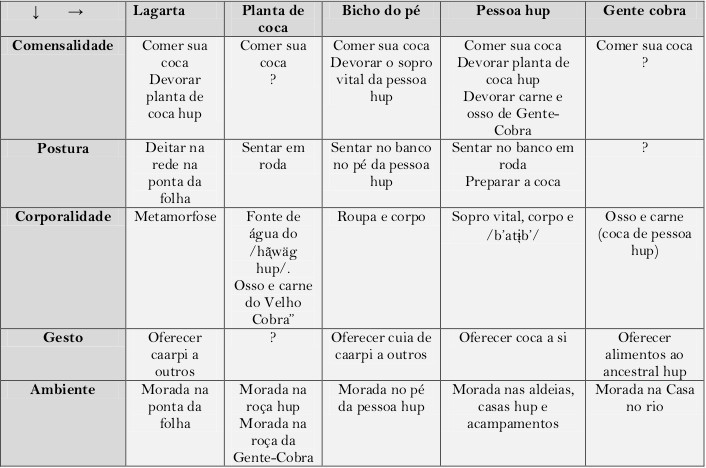
\includegraphics[width=\textwidth]{./img/q1}
%\caption{Quadro de ações relacionadas}
%\end{figure}

% Please add the following required packages to your document preamble:
% \usepackage{booktabs}
% \usepackage{graphicx}

% Verificar tabela.
% \begin{table}[]
% \centering
% \resizebox{\textwidth}{!}{%
% \begin{tabular}{@{}llllll@{}}
% %\toprule

% \textbf{↓ →} & \textsc{lagarta} & \textsc{planta de coca} & \textsc{bicho"-de"-pé} & \textsc{pessoa hup} & \textsc{gente-cobra} \\ 

% \midrule

% \textit{Comensalidade} & \begin{tabular}[l]{@{}l@{}}Comer sua \\ coca\\ Devorar planta\\ de coca hup\end{tabular} & \begin{tabular}[l]{@{}l@{}}Comer sua \\ coca\\ ?\end{tabular} & \begin{tabular}[l]{@{}l@{}}Comer sua\\ coca\\ Devorar o sopro\\ vital da pessoa\\ hup\end{tabular} & \begin{tabular}[l]{@{}l@{}}Comer sua\\ coca\\ Devorar planta\\ de coca hup\\ Devorar carne e\\ osso de Gente-Cobra\end{tabular} & \begin{tabular}[l]{@{}l@{}}Comer sua\\ coca\\ ?\end{tabular} \\ \midrule
% \textit{Postura} & \begin{tabular}[l]{@{}l@{}}Deitar na rede\\ na ponta da \\ folha\end{tabular} & \begin{tabular}[l]{@{}l@{}}Sentar em\\ roda\end{tabular} & \begin{tabular}[l]{@{}l@{}}Sentar no banco\\ no pé da pessoa\\ hup\end{tabular} & \begin{tabular}[l]{@{}l@{}}Sentar no banco\\ em roda\\ Preparar a coca\end{tabular} & ? \\ \midrule
% \textit{Corporalidade} & Metamorfose & \begin{tabular}[l]{@{}l@{}}Fonte de água do\\  \textit{hã̖wäg hup}\\ Osso e carne\\ do Velho Cobra\end{tabular} & Roupa e corpo & \begin{tabular}[l]{@{}l@{}}Sopro vital, corpo \\ e \textit{b'atɨ̖b'}\end{tabular} & \begin{tabular}[l]{@{}l@{}}Osso e carne\\ (coca de pessoa\\ hup)\end{tabular} \\ \midrule
% \textit{Gesto} & \begin{tabular}[l]{@{}l@{}}Oferecer caarpi\\ a outros\end{tabular} & ? & \begin{tabular}[l]{@{}l@{}}Oferecer cuia\\ de caarpi a outros\end{tabular} & Oferecer coca a si & \begin{tabular}[l]{@{}l@{}}Oferecer alimentos\\ ao ancestral hup\end{tabular} \\ \midrule
% \textit{Ambiente} & \begin{tabular}[l]{@{}l@{}}Morada na ponta\\ da folha\end{tabular} & \begin{tabular}[l]{@{}l@{}}Morada na roça\\ hup\\ Morada na roça\\ da Gente-Cobra\end{tabular} & \begin{tabular}[l]{@{}l@{}}Morada no pé\\ da pessoa hup\end{tabular} & \begin{tabular}[l]{@{}l@{}}Morada nas aldeias,\\ casas hup e \\ acampamentos\end{tabular} & \begin{tabular}[l]{@{}l@{}}Morada na Casa\\ no rio\end{tabular} \\ \bottomrule
% \end{tabular}%
% }
% \caption{Quadro de ações relacionadas.}
% \label{my-label}
% \end{table}                                        

\section{Sentar e deitar}\label{sentar-e-deitar}

\index{ab@\textsc{b}1\quad \textit{Pũ'ũ̖k bi'i̖d}\break Benzimento da coca}
Os benzedores hup não usam maracás ou cocares quando praticam um
encantamento, mas procuram geralmente sentar"-se em bancos. Para o ato
coletivo de comer coca, os participantes procuram também assumir a
postura sentada, seja em bancos, seja sobre folhas ou no chão. Proteger
a pessoa hup para o consumo da coca envolve fazê"-la sentar"-se no
\textit{primeiro banco} à noite, como os senhores hup, e não permitir que ela
fique \textit{deitada na rede} durante o dia como a lagarta e nem que ela
aceite beber seu \textit{caarpi} (\textsc{b1}). Partindo das reflexões de Ingold
e Kendon, entendo a postura como um alinhamento corporal para a ação.
Percebo que os modos de sentar e os modos de deitar contribuem para a
diferenciação dos seres quanto a suas perspectivas. Essa diferenciação
protege também dos perigos das metamorfoses.

Os bancos são feitos com madeira de ``sorva'',\footnote{\textit{Pãhã̗y},
  ``sorva'', árvore da família das apocináceas, \emph{Couma guianensis}.
  Cf. Ramirez (2006).} \textit{pãhã̗y}, árvore encontrada na mata próxima à
comunidade. Fabricados a partir de uma mesma peça de madeira, que é
entalhada a terçado, os bancos demoram aproximadamente quatro horas para
ficarem prontos. São leves, pequenos, fáceis de carregar de um lugar
para outro.\footnote{Creio que o design e a técnica empregada diferenciam
  os bancos hup dos bancos dos Tukano, que são mais pesados e demoram em
  média 72 horas para serem fabricados, segundo a Tok Stok. São,
  portanto, de fabricação muito mais rápida, pois um Hup usa somente
  5,5\% do tempo que um Tukano leva para fazer seu banco (ver
  \textless{}\emph{http://tokstok.com.br/linhakumurõ}\textgreater{}).} Além disso, os bancos hup não
são polidos ou lixados e nem recebem grafismo de trançado como os bancos
tukano. São fabricados também bancos pequenos para as crianças e seus
tamanhos variam de acordo com suas idades. Os homens aprendem a fazer os
bancos com seus pais, sendo uma das primeiras peças do mobiliário da
nova morada do casal após o casamento, junto com as redes.

A pedido de pais e avós, os benzedores muitas vezes realizam as práticas
para proteger ou curar enquanto participam das rodas de coca. Sentados
nos ``bancos hup'', \textit{hup kä̖d}, os senhores executam os encantamentos. É
marcante o contraste entre, por um lado, o corpo silencioso, quase
imóvel, concentrado, os lábios movimentando"-se próximos ao cigarro ou à
cuia, soprando"-os para fazer as palavras penetrarem, gesticulando as
mãos para reforçar ações mencionadas e, por outro, sua pessoa"-sopro
(pensamento ou sopro vital) em constante movimento pelo cosmos, entrando em
relação com seres e com outras dimensões do espaço"-tempo.

Como disseram, nas rodas os benzimentos nunca são contados por completo.
Quando o encontro está prestes a terminar, os senhores enchem suas bocas
de coca, despedem"-se e vão para suas casas para deitar na rede. Enquanto
a coca vai sendo absorvida, os senhores deslocam seu ``pensar'',
\textit{wä'kë̗y}, e seu ``sopro vital'', \textit{hã̗wäg}, para os tempos e espaços
mencionados nas conversas da roda. Esse é um momento perigoso, pois os
benzedores e pajés de todas as Casas do Céu, da Terra, do Rio, do
Subterrâneo, de outras comunidades hup e de outras etnias estão
deslocando"-se para ``roubar'', \textit{s'ë̗kë̗y}, os encantamentos, o sopro
vital, e os ``saberes'', \textit{hipã̗hã̗y}, uns dos outros. Para estar
protegido, é preciso que o benzedor saiba cercar"-se com o ``benzimento
de cercar os sonhos'', o \textit{sõh ni̗ ta̗' bi'i̖d}, e manter"-se acordado. Do
contrário, terá sonhos ruins que podem representar perigo à sua família
e à aldeia como um todo. Por volta das duas da madrugada os benzedores
dizem dormir e sonhar. Em seus sonhos, deslocam"-se para as casas onde
estão seus pais, avós e ancestrais. Esses surgem e contam os
encantamentos e mitos sobre os quais conversavam na roda. Assim, os
viajantes hup conseguem complementar as sequências de ações parcialmente
descritas nos encontros noturnos.

Antigamente, contam os senhores hup, suas redes eram feitas de ``fibra
de tucum'',\footnote{Tucum, palmeira da família das arecáceas,
  Astrocaryum tucuma, Cf. Ramirez, 2006.} \textit{k'öb"-s'o̗}, palmácea
encontrada hoje em dia em áreas de floresta mais distantes das aldeias.
Por meio das trocas com os comerciantes e com os religiosos, os Hupd'äh
passaram a adotar as redes de pano dos brancos. Cada pessoa possui sua
própria rede. Apenas bebês e crianças pequenas ocupam a mesma rede das
mães, pais ou irmãos mais velhos. Adultos partilham a mesma rede para
relações sexuais ou para o consumo de caxiri em dias de festa. Como
visto em \textsc{b1}, deitar"-se na rede permite aconchegar"-se em meio ao \textit{calor
gostoso} para o descanso, \textit{bɨ̗'nɨ̗h}, ``não fazer'', e para o ``sono'',
\textit{õ̗h}. Mas, após as rodas de coca, é justamente esse descanso e sono,
ainda com a coca na boca, que possibilitam a viagem da pessoa hup que se
dá durante o repouso do \textit{sa̗p}, ``corpo'', e na concentração e movimento
como pessoa"-sopro (sopro vital ou pensamento). Tomando a reflexão de Lolli,
há assim uma desconstrução da pessoa e uma concentração num regime de
corporalidade diferente.\index{ab@\textsc{b}1\quad \textit{Pũ'ũ̖k bi'i̖d}\break Benzimento da coca}

As posturas de \textit{hipe̗me̗y}, ``sentar'', e de \textit{ya̗ga̗t}, ``deitar"-se na
rede'', são alinhamentos corporais importantes para \textit{viajar},
interagir com outros seres e adquirir mais habilidades para curar ou
proteger. Pajés e benzedores contam sempre sobre sonhos em que viajam
com seus \textit{hã̗wäg"-wä'kë̗y} para as diversas casas do cosmos, morros,
cachoeiras, lagos. É como \textit{ham k'ö̗'}, ``viagem'', que essa mobilidade do
ser é percebida. Através desse deslocamento, os xamãs estabelecem
relações com ancestrais e seres diversos que habitam os muitos
planos"-casa do universo. É por meio dessa mobilidade e fluidez --- para
tomar conceitos chave através dos quais Silverwood"-Cope, Reid e Pozzobon
refletiram sobre a organização social e a circulação de Hupd'äh,
Yuhupdëh e Kákwa pelo território --- que o xamã interage com as múltiplas
perspectivas e busca situar"-se para intervir no campo de percepção e
ação dos seres, agindo para alterar suas percepções sensoriais e acalmar
sua fúria. Também para Lolli, a concepção yuhup de pensamento diz
respeito à ação e ao deslocamento. Em suas palavras,

\begin{quote}
O que gostaria de frisar é que pah"-këy me sugere ao mesmo tempo uma
distinção entre planos distintos de atuação e a possibilidade de
atravessar os planos conectando"-os, já que se age alhures para agir
aqui: através de pah"-këy, a atuação em um plano é também a atuação em
outros planos.\footnote{2010, p.\,72.}
\end{quote}

Conversando muitas noites com Jovino e seu pai, Ponciano, disseram"-me
que o ``benzedor'', \textit{bi'i̖d ĩh}, enquanto profere o benzimento,
murmurando"-o em direção a um objeto intermediário, \textit{Tɨ̗h hã̗wäg ham. Tɨ̗h
wä'kë̗y ham. Bab' ni̗}, ``Vai como pensamento. Vai como sopro vital.
Juntos.'', dirige"-se até a pessoa a ser benzida e depois desloca"-se para
as diversas Casas do Céu, da Terra, do Rio, do Subterrâneo, dependendo
do encantamento. O deslocamento se daria não \textit{em pensamento}, mas
\textit{como pensamento}, estando o pensamento sempre acompanhado do \textit{sopro
vital} para vibrar e se deslocar num mesmo pulsar.

A antropóloga Dominique Buchillet termina sua tese \emph{Maladie et
memoire des origines chez les Desana du Uaupes} abrindo os seguintes
questionamentos:

\begin{quote}
Entendendo que a eficácia terapêutica repousa no encantamento, e que as
palavras desse encantamento refletem a ideia de um deslocamento no
espaço, uma progressão do kubu de um local a outro para identificar os
agentes responsáveis pela doença, poderíamos nós, portanto, falar de uma
viagem do kubu?\footnote{1983, p.\,198.}
\end{quote}

As perguntas colocadas pela autora sobre o deslocamento do kubu durante
a realização de encantamentos partem de sua minuciosa descrição das
práticas xamânicas dos Desana. A partir de sua etnografia, Buchillet
contrapõe"-se às descrições generalizantes de Lévi"-Strauss e Eliade, por
perceber que as práticas de cura desana são realizadas muitas vezes sem
a presença do doente, em silêncio, por meio de palavras murmuradas e
sopradas em objetos intermediários, sem ornamentos rituais e sem a
\textit{viagem da alma}. A descrição de Reid revela um entendimento da
prática xamânica muito próximo ao de Buchillet. Os encantamentos hup são
vistos pelo autor como fórmulas murmuradas por benzedores ou pajés para
um cigarro ou cuia com remédio líquido. Têm como objetivo a proteção ou
a cura de determinada doença. A \emph{performance} é descrita como a
recitação de um texto cuja estrutura se divide em níveis (chão, centro e
topo).\footnote{No primeiro nível (chão), o benzedor isola a fonte da
  doença. Depois há ações de despoluição e tentativas de libertar o
  espírito da caixa do agente maléfico. Por fim, a alma do paciente é
  recolocada no corpo e as essências ruins são jogadas para fora e
  purificadas (Reid, 1979, p.\,176-7).} A ênfase no caráter textual e
figurativo dos encantamentos torna pouco visível a relação entre o ato
de fala, a postura e a gestualidade do benzedor em suas ações. O
murmúrio e o sopro são os únicos gestos descritos nessa tentativa de
distanciar"-se do modelo de eficácia simbólica levistraussiano. De modo
distinto, creio que tomar os encantamentos como sequências de ações
possa gerar novos entendimentos sobre essa prática. Por um lado, se o
xamã \textit{vai como pensamento e como sopro vital}, há uma ação de
deslocamento da pessoa sentada, murmurando e soprando palavras a objetos
intermediários visando à proteção ou à cura. Por outro lado, quando já
estão deitados em suas redes é que os \textit{comedores de coca} viajam para
os diversos planos"-casa e, como dizem os Hupd'äh, ``trabalham'', \textit{bɨ̗'}.

No banco ou na rede, sentados ou deitados, benzendo ou sonhando, os
xamãs perfazem"-se pessoas"-sopro para viajar ao longo do mundo vivido.
Tornam"-se seres transicionais que são seus próprios movimentos
realizados no \emph{entrecurso} de perspectivas, paisagens, percepções e
sensibilidades. Passa a ser difícil delimitar onde a pessoa"-sopro começa
ou onde acaba, pois ela depende das relações externas que a estabelecem
como um ponto de referência de si para lançar"-se alhures. Os benzimentos
deixam assim de ser tomados apenas como textos recitados para a cura,
podendo ser vistos como sequências de atos realizados através do
deslocamento e da interação com outros seres e lugares para curar ou
proteger.

Pensando com Lolli, esse \textit{devir pessoa"-sopro} é marcado por
procedimentos de desconstrução e reconfiguração de si para a ação
através de uma corporalidade outra que permite ver, ouvir,
movimentar"-se, oferecer, acalmar, banhar, sentar, gestos e posturas para
situar"-se entre o aqui e o lá das muitas moradas (planos"-casa),
paisagens, caminhos e morros. O espírito parece não ser a parte de um
todo, permanentemente alojado no interior do corpo ou um conteúdo
libertado oniricamente. No lugar de ver, como Reid, a agência xamânica
marcada por uma \textit{saída do espírito do corpo para a atuação no universo
não material}, entendo esses movimentos do ser como viagens realizadas
a partir da reconfiguração do xamã como \textit{pessoa"-sopro} (sopro vital e
pensamento), numa transdução para agir mobilizando a energia do contínuo
entre corpo e espírito, entre ego e alter, situando"-se como viajantes ao
longo dos caminhos.

\index{ab@\textsc{b}1\quad \textit{Pũ'ũ̖k bi'i̖d}\break Benzimento da coca}
Toda essa movimentação surge nas \textit{exegeses de benzimentos}, como em
\textsc{b1}, através da narrativa das ações do benzedor quando este
interage com os diversos planos"-casa e com as diversas perspectivas dos
seres que habitam esses locais. Se a viagem da pessoa hup parece ocorrer
a partir de duas posturas corporais específicas: \textit{sentado no banco} e
\textit{deitado na rede}, impedir que a \textit{pessoa fique só deitada na rede
como a lagarta} e fazê"-la sentar"-se no \textit{primeiro banco} talvez sejam
formas de negar o ``não fazer'', o \textit{bɨ̗' nɨ̗h}, modo como a maior parte
das pessoas percebem o \textit{deitar na rede} e inserir o novo \textit{comedor de
coca} num processo de \textit{bɨ̗'}, ``fazer'', ``agir'', que ocorre nos atos
de deitar e sentar. Por outro lado, \textit{fazer sair da rede} talvez impeça
o alinhar da postura a partir da ação da lagarta, o que faria a pessoa
assumir não só o ponto de vista desse ser como também o modo de ação a
partir do qual a lagarta perfaz"-se xamanicamente em sua metamorfose
para, como mariposa, deslocar"-se pelo mundo.

\section{Oferecer}\label{oferecer}

``Oferecer'', \textit{k'o̗po̗y}, vem a ser um gesto fundamental na sequência de
ações de preparo e consumo da coca nos encontros noturnos. De modo
semelhante ao que mostra Buchillet para os Desana, também para os
Hupd'äh muitas doenças relacionadas aos animais e seres malfazejos
ocorrem quando a pessoa aceita seus oferecimentos de alimentos, bebidas
e demais substâncias. Como visto na viagem à Serra Grande, quando um
caminhante chega a uma casa ou aldeia, depois dos cumprimentos, há o
oferecimento imediato de alimentos e bebidas. Em festas de caxiri, a
recusa da bebida oferecida por uma mulher pode significar uma ofensa
grave e, por vezes, ocasionar brigas. Assim, na interação entre pessoas
hup, a recusa a um oferecimento é mal"-vista.

Contrariamente, é a recusa ao oferecimento que permite a proteção da
pessoa hup quando em face a outros seres. Esse é o caso do oferecimento
da cuia de caapi pela lagarta da coca ou pelo bicho"-de"-pé que pode fazer
com que a pessoa hup enlouqueça. Já em \textsc{m9}\index{18@\textsc{m}9\quad História de \textit{Wed B'ö̖'}}, o oferecimento do
caxiri, da coca e dos diversos alimentos pela Mulher Peixe a seu marido
faz com que \textit{Wed B'ö̖'} vomite e desmaie. Também na história de Matumã,
depois de ter ido para a aldeia das Gentes"-Onça, a mãe retorna e oferece
alimento aos filhos (\textsc{m8}). Nas narrativas e nos benzimentos o
gesto de oferecer surge como um movimento que cria ou recria relações
entre as pessoas e as perspectivas.\index{17@\textsc{m}8\quad A história de Matumã}

Nas rodas de coca, o gesto de ``oferecer'', \textit{k'o̗po̗y}, marca toda uma
forma relacional dos encontros noturnos. Como pôde ser percebido na
descrição do preparo da coca, há uma divisão dos papéis e há também uma
diferenciação do \emph{status} dos participantes. Ponciano é chamado de
\textit{yo'o̖m ĩh}, o dono da comunidade de \textit{Ta̗t"-Dëh}, o capitão velho. Seus
pais e seu avô foram os \textit{kɨhsä̗t} que chamaram as outras famílias para
mudarem"-se e formarem a comunidade de \textit{Ta̗t"-Dëh}. Ele e seus irmãos são
reconhecidos como sendo os descendentes dos primeiros \textit{Sokw'ä̗t Noh K'öd
Tẽ̖h d'äh}. Foram esses os primeiros ancestrais hup a sair da
Cobra"-Canoa, \textit{M'e̖h"-Ho̗h"-Tëg}, quando ela fez a viagem trazendo os
diversos clãs hup do Lago de Leite, \textit{Pu̗d"-Dëh"-Moh}, para habitarem as
terras do rio Uaupés. Entre seus consanguíneos, ele é o \textit{sät}, o ``irmão
maior'', de quem é esperado que chame as ações. Para morar em \textit{Ta̗t"-Dëh},
é preciso que a família peça permissão a esse dono. Do mesmo modo, para
abrir uma roça, pescar em igarapés próximos ou caçar, deve ser feito um
pedido formal.

Ponciano é também o principal \textit{pũ'ũ̖k yo'o̖m ĩh}, ``dono da coca''. Todos
os seus irmãos são igualmente donos da coca, assim como todos os agnatos
desse clã que começam a comer coca nessa aldeia. Os \textit{Sokw'ä̗t Noh K'öd
Tẽ̖h d'äh} possuem o maior número de roças, bem como têm acesso aos
melhores igarapés para pescaria e a territórios privilegiados para a
caça. No que diz respeito à coca, suas roças são as maiores e com mais
variedades dessa planta. Os ramos, na maioria das vezes, foram recebidos
dos pais e avós, mas podem também ter sido adquiridos dos sogros e
cunhados.

Ponciano herdou de seu pai o pilão, \textit{pũ'ũ̖k tö̖k}, e também o hábito de
comer coca. É em torno desse pilão que se realizam os principais
encontros noturnos. Contou"-me que passou a sentar"-se com os benzedores e
a comer coca quando tinha por volta de 30 anos. Só começou a benzer
quando tinha perto de 40 anos. Sempre que está em \textit{Ta̗t"-Dëh}, dirige"-se
todas as noites para a roda, senta"-se e espera. É ele quem muitas vezes
começa a contar mitos e a descrever ações de benzimento, sendo sempre
complementado pelos demais. Apesar de não participar da produção da
coca, é comum vê"-lo sair da aldeia para colher coca em sua roça ou nas
de seus irmãos. Seu pote de coca é geralmente abastecido e oferecido por
seu irmão menor, Vicente. Os homens que chegam de viagem vão até ele
para saudá"-lo.

Seu ``cunhado'', \textit{yo̖h}, Firmiano, é também seu \textit{pũ'ũ̖k hɨ̗t ĩh}, seu
``apanhador de coca''. Diz"-se que Firmiano colhe coca para preparar para
ele. Logo que volta da roça, Ponciano ou seus irmãos penduram o saco com
coca no telhado da cozinha, próximo ao pilão. Depois de seu banho,
Firmiano pega o saco com a coca colhida de sua própria roça, mistura
àquela trazida pelos outros e começa a assar as folhas. Ele é o dono do
\textit{primeiro banco}, o responsável por começar a ação de preparo para que
os \textit{donos da coca} possam oferecer o alimento a todos. Caso haja um
novo \textit{comedor de coca}, ou um senhor de clã afim e de outra
comunidade, esse será encarregado do preparo, sendo sempre observado
pelo dono do \textit{primeiro banco}. São os \textit{pũ'ũ̖k hɨ̗t ĩh}, ``apanhadores'',
dos outros donos que contribuirão também com o processo de produção. Sem
possuir potes pequenos, pilões ou grandes roças de coca, aos
\textit{apanhadores} cabem quase todos os dias a colheita da coca e o seu
preparo. Já a colheita dos donos é complementar, sendo suas as sobras do
alimento de um encontro.

São os donos de posição hierárquica inferior que se levantam para
oferecer o pote ao dono de \emph{status} superior presente. Muitos donos
com diferentes \emph{status} podem estar sentados, mas será considerado o
dono da roda em uma noite específica o \textit{pũ'ũ̖k yo'o̖m ĩh ma̗h}, o ``dono da
coca mais próximo'' à cuia, ou seja, ao \textit{primeiro banco}. Em noites
com poucos participantes, alguns donos mais novos ou de posição inferior
integram"-se ao processo seguindo uma ordem de irmandade
(\emph{sibling}). Todo o processo de preparação transforma a coca em
alimento para que ela seja derramada no pote pequeno dos donos, únicos
possuidores desses potes. A preparação da coca é assim dividida de
acordo com critérios de \emph{status} e por um princípio de anterioridade,
onde a ordem de nascimentos,\footnote{Como observa Fausto em 2008, p.\,349.} para o
Alto Rio Negro, ``serve como régua sociocósmica para marcar diferenças
entre segmentos''.

Os \textit{donos da coca} devem fornecer os meios para que os \textit{apanhadores}
colham e preparem o alimento. Muitas vezes os \textit{apanhadores} vão às
roças de seu \textit{dono} ou dos irmãos do dono fazer a colheita. Os
instrumentos de preparo (pilão, panela e cuia) são também pertencentes
ao principal dono de coca de uma roda. Cabe também aos donos oferecer a
coca a todos os participantes enquanto eles conversam, determinar o
sentido de circulação e o momento de término do encontro. Após receber
seu pote com as sobras, o dono diz: \textit{we̖d toho̗y ay}, a \textit{comida
terminou}, todos se levantam, se despedem e se dirigem para suas casas.
Se os \textit{apanhadores} não forem cunhados reais, eles serão sempre afins
classificatórios tendo como referência as relações clânicas. Há também
certa equivalência em termos de grupo etário. Tanto o \textit{dono da aldeia} como os \textit{donos da coca} parecem
designar pessoas magnificadas capazes de ações eficazes, constituindo
uma singularidade plural. As rodas de coca, ao situarem a relação
\textit{dono"-apanhador} estabelecem, assim, a reflexividade performática de
um tipo de relação maestria"-domínio.

Pensando com Houseman e Severi em torno do gesto de oferecer, há uma
dinâmica constante de interações entre os participantes através de
relações de amizade formal. A partir do binômio \textit{dono} e
\textit{apanhador}, um laço específico é criado entre todos, em função da
coca. Há uma transformação na identidade dos participantes que se
estabelece através da articulação entre as relações de parentesco e as
relações da coca. ``Afins'', \textit{yo̖h}, tornam"-se \textit{apanhadores}, enquanto
os ``agnatos'', \textit{yawa̗m}, passam a ser \textit{donos da coca}. Essas
modificações permitem perceber uma condensação ritual, já que, numa dada
sequência de ações, existe uma associação específica de modos de
relação. Nesse sentido, realiza"-se um circuito de dádiva, visto que a
maioria dos participantes colhe e prepara a coca para dá"-la ao dono, ao
passo que este a recebe concentrada em seu pote, que, por sua vez,
concentra também o resultado dos trabalhos de todos. A partir de seu
pote pequeno é que ele retribui a todos, oferecendo a coca que circula
na roda. Nessa articulação entre dono"-pote há uma relação
conteúdo"-continente que marca uma forma de englobamento característica
da assimetria desse modo de domínio.

% \begin{center}
% \textsc{binômio relacional:}
% \textit{pũ'ũ̖k yo'o̖m ĩh} : \textit{pũ'ũ̖k hɨ̗t ĩh}
% dono da coca : apanhador da coca
% \end{center}

%\begin{figure}
%\centering
%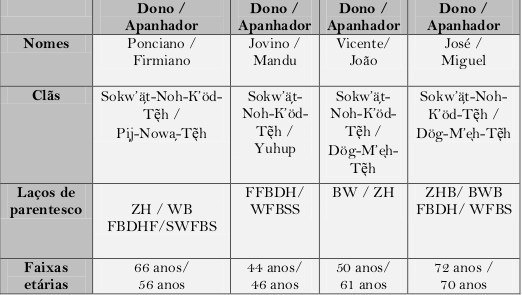
\includegraphics[width=\textwidth]{./img/q2}
%\caption{Quadro de relações entre donos e apanhadores}
%\end{figure}

% Please add the following required packages to your document preamble:
% \usepackage{booktabs}
% \usepackage{graphicx}
% Please add the following required packages to your document preamble:
% \usepackage{booktabs}
% \usepackage{graphicx}
% Please add the following required packages to your document preamble:
% \usepackage{booktabs}
% \usepackage{graphicx}

% Verificar essa tabela.
% \begin{table}[]
% \centering
% \resizebox{\textwidth}{!}{%
% \begin{tabular}{@{}lllll@{}}
% %\toprule
% \textbf{} & \textit{Dono/\,Apanhador} & \textit{Dono/\,Apanhador} & \textit{Dono/\,Apanhador} & \textit{Dono/\,Apanhador} \\ \midrule
% \textbf{Nomes} & Ponciano/\,Firmino & Jovino/\,Mandu & Vicente/\,João & José/\,Miguel \\ 
% \midrule

% \textbf{Clãs} & \begin{tabular}[c]{@{}c@{}}Sokw’ä̗t-Noh-K’öd-\\ Tẽ̖h/\,Pi̖j-Nowa̗-Tẽ̖h\end{tabular} & \begin{tabular}[c]{@{}c@{}}Sokw’ä̗t-Noh-K’öd-\\ Tẽ̖h/\,Yuhup\end{tabular} & \begin{tabular}[c]{@{}c@{}}Sokw’ä̗t-Noh-K’öd-\\ Tẽ̖h/\,Dög-M’e̖h-Tẽ̖h\end{tabular} & \begin{tabular}[c]{@{}c@{}}Sokw’ä̗t-Noh-K’öd-\\ Tẽ̖h/\,Dög-M’e̖h-Tẽ̖h\end{tabular} \\ 

% \midrule

% \textbf{\begin{tabular}[c]{@{}c@{}}Laços de parentesco\end{tabular}} & \begin{tabular}[c]{@{}c@{}}\textsc{zh/\,wb}\\\textsc{fbdhf/\,swfbs}\end{tabular} & \textsc{ffbdh/\,wfbss} & \textsc{bw/\,zh} & \begin{tabular}[c]{@{}c@{}}\textsc{zhb/\,bwb}\\ \textsc{fbdh/\,wfbs}\end{tabular} \\ 
% \midrule
% \textbf{\begin{tabular}[c]{@{}c@{}}Faixas\\ etárias\end{tabular}} & 66--56 anos & 44--46 anos & 50--61 anos & 72--70 anos \\ \bottomrule
% \end{tabular}%
% }
% \caption{Quadro de relações entre donos e apanhadores.}
% \label{my-label}
% \end{table}

Hugh"-Jones e Buchillet mostram em suas descrições das rodas de coca que
elas são fundamentais para a transmissão de substâncias e conhecimentos
entre agnatos. De modo diferente, creio que as rodas realizadas pelos
Hupd'äh apontem para uma diferença quanto a esses eventos e à circulação
de saberes, pessoas e substâncias. Como na descrição de Silverwood"-Cope
das rodas de coca kákwa, agnatos e afins participam conjuntamente dos
encontros noturnos já que coabitam um mesmo grupo local. A constância
nessa dinâmica de interação permite ver que os participantes se
organizam em função da sequência de ações entre \textit{donos de coca} e
\textit{apanhadores}.

% Verificar tabela.
% \begin{figure}
% \centering
% 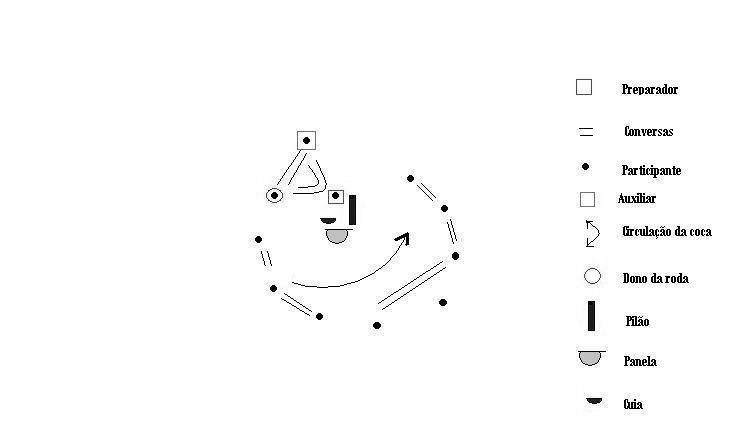
\includegraphics[width=\textwidth]{./img/010}
% \caption{Esquema de relações posicionais numa roda de coca.}
% \end{figure}

Conversando entre ``irmãos'', \textit{yawa̗m}, ou entre ``afins'', \textit{yo̖h}, os
\textit{comedores de coca} adquirem habilidades e mostram uns aos outros
sentidos que estão no mundo, sendo estes revelados pelas viagens e
interações com ancestrais, animais e outras gentes. O perigo na oferenda
da lagarta talvez esteja no fato de, aceitando o \textit{caarpi}, a pessoa hup
além de consumir a substância, aceita situar"-se num modo de relação com
esse ser e abandonar sua posição e seu fazer na roda de coca e no mundo
hup. Isso gera o perigo de roubo de seus conhecimentos, saberes e
habilidades xamânicas. Afinal, parece não haver possibilidade de
consumir a coca sem tomar parte nas ações de preparo e aquisição de
habilidades que diferenciam os participantes em termos da organização,
\emph{status} e saberes. Como nas caminhadas, entendo que as rodas de
coca perfazem o contexto para uma educação da atenção. Sentados ou
deitados em suas redes, os senhores hup manejam a coca enquanto potência
primordial e adquirem habilidades de modo diferenciado. A partilha da
coca é também um processo de potenciação de habilidades de cura e
proteção que se articula em relações diferenciais entre os
participantes. Através desse modo de ação, processos de magnificação de
pessoas articulam"-se performativamente.

\section{Palavras}\label{palavras}

A hierarquia da roda é também uma hierarquia da palavra. Apenas
Ponciano, Paulino e o pajé Armando podem contar para mim, \textit{branco
pesquisador}, ou para um Tukano ou Desano, índios de outras etnias,
histórias e benzimentos. A posição que ocupam, a idade, seus saberes e a
eficácia de suas ações de cura e de proteção fazem com que sejam
considerados grandes conhecedores das \textit{pɨnɨ̖g}, ``histórias'', e dos
benzimentos. Apesar disso, enquanto contam, esses narradores fazem
perguntas a seus cunhados e apanhadores. Os afins participam e
complementam suas narrativas. Isso torna as versões de mitos contadas e
as descrições de ações xamânicas pontos de convergência de saberes de
diferentes clãs.

Tomando como referência a etnografia da fala, é possível dizer que,
quando a coca começa a circular, os participantes conversam através do
que denominam ser a \textit{hib'a̗h ɨ̗d}, a ``fala da origem'', e também da
\textit{bi'i̖d ɨ̗d}, a ``fala dos benzimentos''. Dessa forma, comentários sobre o
desempenho na execução de um benzimento, contar partes de algum
encantamento a alguém ou mesmo o ato de benzer compõem essa \textit{linguagem
dos benzimentos}. Já as histórias sobre \textit{K'e̖g Tẽh}, \textit{K'e̖g Tẽh pɨnɨ̖g},
sobre os ``ancestrais'', \textit{hib'a̗h tẽh d'äh pɨnɨ̖g}, ou sobre os
``antigos'', \textit{wähä̗d däh pɨnɨ̖g}, podem ser tomadas como gêneros dessa
\textit{fala da origem} por meio dos quais são narradas as ações desses
seres.

Os encontros noturnos podem, a meu ver, ser entendidos de modo muito
semelhante ao que Gow mostra ser uma \emph{mitopoiesis}. O
envelhecimento dos homens ocorre simultaneamente à sua participação nas
rodas de coca. A autoridade para contar mitos e para executar práticas
xamânicas tem como referência os \textit{antigos} e sua participação em rodas
de coca \textit{s'a̗m yɨ}, desde ``muito tempo atrás''. Se ao longo da vida uma
pessoa ouviu histórias e encantamentos de seus pais ou parentes
próximos, as rodas situam o contexto e o enquadramento performático para
a expansão em profundidade e complexidade, permitindo a cada um, a
partir de diálogos, tecer mais detalhes e conexões.

Como me contaram, é quando possui filhos ``rapazes'', \textit{pesa̖w d'äh}, e
``moças'', \textit{ta'asa̗w d'äh}, que os homens e mulheres começam a ser
denominados \textit{wähä̗d'd'äh}, ``velhos''. O casamento dos filhos e o
nascimento dos netos também podem marcar a designação dos pais como
\textit{wähä̗d'd'äh}. Como mostra Reid, a categoria inclui desde os mais velhos
da geração vivente até ancestrais míticos. Com o envelhecimento ocorre
um aumento da atuação dos velhos na vida ritual e política da
comunidade. São os anciões que conduzem os assuntos do grupo local,
sendo sempre consultados quanto aos melhores lugares para caçar, pescar
e abrir roças. A eles cabe o papel importante de aconselhar os mais
jovens e sugerir ações e decisões com relação à vida política e ritual.
Cuidar dos netos é uma atividade que ocupa boa parte de seu dia a dia.
Pela manhã é comum encontrar avós nas casas com as crianças,
ensinando"-lhes a tecer cestos, paneiros, tipitis e demais instrumentos
de trabalho. Tanto as senhoras como os senhores contam narrativas
míticas aos netos, ensinam cantos e brincadeiras.

Comer muita coca, passar por muitos eventos rituais, conhecer
detalhadamente narrativas míticas e ações xamânicas gera alterações na
composição corporal. Em crescimento ao longo da vida, o \textit{sopro vital}
atinge o tamanho do próprio corpo na velhice. Nesse processo de mudança,
há também um aumento do poder dos \textit{wähä̗d d'äh}, que os torna mais aptos
para as viagens xamânicas e para a interação com outros seres e
planos"-casa. Para aqueles que vivem junto ou próximo aos velhos, isso é
percebido beneficamente, mas o risco da prática da feitiçaria pelos
\textit{wähä̗d d'äh} de grupos locais diferentes e distantes gera temor. É
primeiro a seus pais e sogros que uma pessoa pede um benzimento. Caso
esse não tenha eficácia, o pedido será feito a um benzedor de
\emph{status} superior ou a um dos pajés. Quando querem ouvir ou
relembrar uma narrativa mítica, é também a pais e avôs que uma pessoa
pergunta primeiro, para depois procurar narradores de outros \textit{kakah},
``grupos de fogo'', ou clãs.

Analisando as relações entre benzimentos e mitos yuhup, Lolli mostra que
o benzedor e alguns heróis míticos, agindo entre planos"-casa e múltiplas
perspectivas, têm a função de \textit{conseguir conectar os acontecimentos do
presente aos processos ontogênicos de individuação}. Retomando
\textsc{m9}\index{18@\textsc{m}9\quad História de \textit{Wed B'ö̖'}}, é possível perceber que a \textit{origem da coca} revela a
transição entre perspectivas ocasionada por uma aliança. Hupd'äh e
Gente"-Cobra passam a ser afins, e o pai da moça, uma filha mais velha,
torna"-se um \textit{wähä̗d}, um Velho Cobra. Tomando as palavras de Fausto
(2008, p.\,349),

\begin{quote}
A relação sogro"-genro encontra"-se no polo oposto ao da germanidade, pois
se compõe de diferenças e assimetrias sobrepostas: sobre uma base de
afinidade, erguem"-se duas outras assimetrias, aquela entre
tomador"-doador de mulheres e aquela entre gerações. A relação é potente
demais, logo deslizando para figuras de poder e para a voracidade
canibal.
\end{quote}

A sequência de ações do mito pode ser vista como a transmissão de
benzimentos e de substâncias entre afins pela mediação da Mulher Peixe.
Ao contrário do oferecimento como redistribuição do \textit{dono da coca}, é
a partir de uma reciprocidade negativa, do roubo do \textit{dedo}, \textit{ramo}, que
alimentos e encantamentos surgem para os ancestrais hup. Enquanto no
casamento o esposo deve \textit{me̗y}, ``pagar'', a família da mulher abrindo
roças, pescando ou caçando, na narrativa ocorre uma inversão, já que é a
ação da Mulher Peixe que faz aparecerem as plantações. O pai, dono de
coca e de saberes xamânicos, torna"-se ``velho'', \textit{wähä̗d}, com o
casamento da filha. Sem adivinhar as intenções da moça, ele não consegue
proteger sua coca e seus conhecimentos xamânicos do ``roubo'', \textit{s'ë̗kë̗y}.
A aliança entre a Mulher Peixe e o ancestral hup, o oferecimento dos
alimentos e a aquisição de benzimentos revelam seus perigos no vômito e
desmaio, no surgimento de doenças e na essência ruim da coca, \textit{cera da
vagina de Mulher"-Peixe}, que deve ser extraída para o consumo. A
sobreposição de assimetrias desliza para ``figuras de poder e para a
voracidade canibal''.\footnote{Fausto, 2008.}

Nas narrativas, talvez esses eventos que fazem surgir malefícios e ao
mesmo tempo encantamentos possam ser tomados, por um lado, como
acontecimentos que arrebatam sujeitos, e, por outro, como ações de
manejo de potências primordiais que permitem a determinados sujeitos
agirem para tornar seus pontos de vista predominantes e, assim, gerar
processos ontogênicos de pessoas, alimentos e encantamentos. A Mulher
Peixe advinha a intenção de seu pai de revistar seu corpo e esconde o
dedo ou ramo em sua vagina para depois dar ao ancestral hup a possibilidade
de obter coca. Os preparadores estão cientes da essência ruim da coca,
dos malefícios e doenças que surgem nessa interação com a Gente"-Cobra.
Por isso, realizam o \textit{benzimento da coca} e transformam os processos
de assar a carne, pilar os ossos e salgar o alimento em ações de
aprendizado e atenção. Atuando na mediação entre modos de percepção,
\textit{mulher"-cobra} e \textit{comedores de coca} realizam ações de manejo de
potências primordiais que permitem a eles adivinhar as intenções e
preparar"-se para a espera do ponto culminante em que surgem alimentos,
malefícios e encantamentos. Cotidianamente, as ações perfazem
encantamentos e narrativas e situam um modo de interação com as
Gentes"-Cobra através de ações de roubo e predação, que tomam de assalto
o Cobra em sua passagem para a velhice, quando não está ainda bem
preparado para proteger seus conhecimentos, sua filha e sua coca.

Nesse sentido, as rodas de coca situam o processo de tornar"-se
\emph{mitopoético} dos mais velhos, fazendo com que estes tenham maior
facilidade e habilidade para narrar e executar benzimentos.
Parafraseando Gow, o mito muda conforme o narrador muda de idade e à
medida que participa de mais e mais encontros noturnos durante a vida. À
medida que envelhecem, as pessoas hup passam a ser autoridades vivas e
ativas no conhecimento sobre os antigos e passam a contar as \textit{histórias
dos antigos} apenas com referência à sua autoridade e à dos antigos.

\section{Contar e ouvir}\label{contar-e-ouvir}

Espero ter demonstrado como os processos e as relações das rodas de coca
revelam uma \emph{performance}, uma dinâmica constante de interações
marcada por condensações rituais e por modificações na identidade dos
participantes. As sequências, transformações, passagens entre as
narrativas e eventos performáticos vão constituindo transformações onde
o interesse por ouvir, contar e ver gera aproximações e distanciamentos
entre seres, pessoas, corpos e substâncias nos diversos tempos e espaços
do cosmos através das viagens.

Sentando"-se todas as noites em roda, os velhos assumem perspectivas e
identidades distintas e relacionam"-se como \textit{donos} e \textit{apanhadores} a
partir de um princípio de anterioridade. A organização da ação dá forma
à \emph{performance} e faz circular as palavras, a coca e as pessoas.
Seus diálogos murmurados vão descrevendo linhas e tecendo as vidas
presentes e passadas numa trama expressa por mitos, sonhos e
benzimentos. A partilha da coca e do tabaco entre \textit{donos} e
\textit{apanhadores} é também a partilha de diferentes tipos de coca e
tabaco, dados pelo deus a cada grupo, cultivados e transmitidos por cada
clã e consumidos pelos que falam a mesma língua. Os saberes, benzimentos
e mitos, patrimônios de cada grupo clânico, circulam nesses encontros e
protegem os grupos de fogo e locais da aproximação das ``outras
gentes'', \textit{sã̗p hupd'äh}. Esses outros, humanos, são tanto os
Gente"-Cobra, Gente"-Onça, quanto bichos do pé, lagartas etc., e por isso
é necessário, como nas caminhadas, estar atento aos mínimos sinais de
suas presenças.

Contar mitos e descrever as ações de encantamentos são atos de mostrar.
Fazem os participantes, agnatos e afins, voltarem sua atenção para
sentidos que estão no mundo, nos diversos planos"-casa. O benzimento terá
maior eficácia de acordo com a capacidade do benzedor de viajar como
\textit{pessoa"-sopro} e interagir com diversos seres e ancestrais. Nos
movimentos da coca, dos corpos, das narrativas e das pessoas, os fazeres
ritual e mítico dos benzedores descrevem os contornos de uma
\emph{mitopoiesis} hup que vai reestabelecendo a cada encontro, a cada
cuia e a cada cigarro um equilíbrio tenso ao longo do mundo vivido dos
Hupd'äh.\footnote{Estar atento, como sugere Schouten (2010), a um só
  tempo às \emph{qualidades sensíveis da lógica}, como V. Turner, e à
  \emph{lógica das qualidades sensíveis}, como Lévi"-Strauss, faz"-se
  fundamental para que se possa interpretar essas múltiplas viagens que
  parecem caracterizar os diversos modos de ação desses círculos de
  coca.}

\chapter{Círculos de fumaça}\label{cuxedrculos-de-fumauxe7a}

% \epigraph{
% %\begin{verse}
% Acendo um cigarro ao pensar em escrevê-los\\
% E saboreio no cigarro a libertação de todos \qb{}os pensamentos.\\
% Sigo o fumo como a uma rota própria,\\
% E gozo, num momento sensitivo e competente,\\
% A libertação de todas as especulações\\
% E a consciência de que a metafísica é uma consequência \qb{}de se estar
% mal disposto.
% }{\textsc{fernando pessoa}, ``Tabacaria''}

\setlength{\epigraphwidth}{.60\textwidth}
\begin{epigraphs} 
\qitem{Acendo um cigarro ao pensar em escrevê-los\\
E saboreio no cigarro a libertação de todos os pensamentos.\\
Sigo o fumo como a uma rota própria,\\
E gozo, num momento sensitivo e competente,\\
A libertação de todas as especulações\\
E a consciência de que a metafísica é uma consequência de se estar
mal disposto.}{\textsc{fernando pessoa}, \textit{Tabacaria}}
\end{epigraphs}

\section{\textit{Hũ̖t Wäg"-Mo̖y}, «morada de semente de
tabaco»}\label{a-caminho-da-hut-wuxe4g-moy-morada-de-semente-de-tabaco}

Depois de colhermos coca nas plantações do irmão de Américo, continuamos
caminhando rumo à \textit{K'a̗j"-Pa̖ç}, Serra da Cutivaia. Íamos deixando o
caminho largo das roças e penetrando uma trilha estreita por meio da
qual nos aproximávamos cada vez mais do morro. Havia ainda algumas
plantações da família de Américo. Andávamos rápido e logo já estávamos
próximos à nascente do \textit{K'a̗j"-Dëh}, Igarapé"-Cutivaia, no pé do morro.
Ao cruzarmos o igarapé, Américo apontou o lugar onde seu pai colocava o
pari para pescar: ``Pegava muitos peixes nesse tempo'', lembrou
sorrindo. Seu pai fora o primeiro a chegar à \textit{K'a̗j"-Paç}. Tinha vindo com
a família toda de \textit{B'o̖t"-Pe̗m"-Dëh"-Mo̖y"-Höd}, morada antiga, próxima à
Serra Grande. Logo que chegou, Henrique plantou pimenta, banana, coca.
Tudo cresceu bem no começo. A terra era muito boa para plantar, \textit{M'aj'"-kɨ̗'}, ``terra firme''. Mas logo sopraram um estrago (feitiço). As
plantas começaram a morrer e já não brotou mais nada.

\index{19@\textsc{m}10\quad \textit{U̖y-ta̖k}}
Ainda no caminho, ouvimos o som de um pássaro, \textit{uy"-ta̖k}. (\textsc{m10})
``\textit{U̖y"-ta̖k} é gente antigamente. Tem um irmão menor. Ele é o \textit{sät}.
Depois, não encontrou mulheres. Comeu o irmão menor mesmo. Fez sexo com
ele''. O \textit{u̖y"-ta̖k} que ouvíamos cantava do alto de uma árvore. Estava com
seu filho pequeno. Naqueles dias, Américo e eu colhíamos coca para que
eu levasse a seu irmão Marino. A coca foi assada e pilada por nós nos
outros dias. Em minha viagem de volta a São Gabriel, eu procuraria
Marino para entregar"-lhe esse presente de seu irmão. A coca o faria
lembrar de suas terras, de suas roças, de sua vida em \textit{Ta̗t"-Dëh}.\footnote{Ver capítulo \emph{Viagens a São Gabriel}, p.\,\pageref{viagens}.}

Desde que o velho Henrique faleceu, Marino não voltou mais à sua
comunidade. Ele e a esposa, dona Mariquinha (\textit{Ya'a̗m K'e̖g}, nasc. 1961,
\textit{Dög M'e̖h Te̖͂h}, ind. 41), estavam morando na casa do genro num bairro
periférico de São Gabriel. Suas filhas já viviam na cidade há alguns
anos para estudar. Américo estava muito preocupado, pois diziam que seu
irmão não parava de beber cachaça. Ele trabalhava alguns dias numa
pedreira e em outros cuidava do sítio de sua patroa, funcionária do
\textsc{dsei}"-\textsc{rn}.\footnote{Distrito Sanitário Especial Indígena do Alto Rio Negro
  (\textsc{dsei}"-\textsc{rn}).} Sem falar português e sem documentos, estava ``sofrendo
muito na cidade'', dizia Américo. Segundo ele, seu irmão não sabia
guardar dinheiro, era roubado pelos comerciantes e estava sempre metido
em brigas. Enquanto caminhávamos, ele disse ter ``saudades'', \textit{hot"-ɨ̗d},
de Marino. As lagartas estavam comendo sua coca, suas roças estavam
cheias de mato, e sua casa, abandonada.

Encontramos um pé de cana bem perto do morro e paramos para chupar.
Sentamo"-nos e começamos a ouvir o canto de ``inambus'',\footnote{Inambu,
  \textit{mo̖h}, nome dado a várias espécies de inambus de tamanhos médio e
  grande (família dos tinamídeos). Cf. Ramirez (2006).} \textit{mo̖h}. Américo
assobiava. Dois pássaros cantavam. Aproximavam"-se devagar, vindo em
nossa direção. Mas, de repente, voaram. ``O melhor é chamá"-los logo de
manhã, quando estão bravos. Daí, vêm logo. A essa hora já não vêm
mais'', explicou. Começamos a subir o morro e vimos um buraco fechado.
Era uma casa de paca. A cobertura que tapava o buraco era a porta. ``A
paca fecha a porta para proteger"-se'', disse. Continuamos a subida. Com
o terçado, Américo cortou um cipó grande. Ergueu"-o inclinando a parte
cortada para sua boca e bebeu a água que escorria. Matamos nossa sede.
Essa era uma ``água pura'', \textit{yõ̖h dëh}. O cipó chamava"-se \textit{pa̖ç"-tɨ̗t},
``cipó da serra''. ``Os soldados gostam muito'', comentou, ``dá
força!''.

\index{20@\textsc{m}11\quad \textit{Hu̖͂t Wäg}\break Semente de Tabaco}
Estávamos já no meio do morro quando chegamos a uma \textit{Pa̖ç"-Mo̖y}, Casa de
Pedra, uma gruta. Uma pedra muito grande cobria o buraco que levava
para o interior do morro. Estávamos diante da morada antiga do ancestral
\textit{Hu̖͂t Wäg}, Semente de Tabaco. A rocha erguia"-se como uma cobertura
ampla para o abrigo fresco e bem preparado para a chuva. (\textsc{m11})
Numa roda de coca, Miguel contou que \textit{Hu̖͂t Wäg} era um ancestral dos
Yuhupdëh. Esse ancestral viveu com sua família em muitas Casas de
Pedra.\footnote{Reichel"-Dolmatoff (1996) comenta sobre a importância dos
  morros e casas de pedra para os povos Tukano também. Uma análise mais
  aprofundada sobre essas moradas será feita no capítulo \emph{Caminhos abertos}.} No chão de
terra avermelhada dessas moradas, sempre é possível encontrar as \textit{b'o̗kab
b'a̗h}, as ``lascas de cerâmica'', restos de suas panelas, fornos e
utensílios de cozinha. Sua primeira morada fora a Serra da Cutivaia.
Como o pai de Américo, esse ancestral fora o primeiro a chegar lá.
Depois se mudou para \textit{Ni̗k"-Hu̗͂-Pa̖ç} e posteriormente para \textit{B'ö̖'"-Pa̖ç}. De
lá, ele e a família subiram para o céu. Hoje em dia moram numa casa
próxima à de \textit{K'e̖g Te͂h}.\footnote{Reid comenta também sobre a proximidade
  de habitação celeste entre \textit{Hũ̖t Wäg, K'e̖g Tẽh} e outros ancestrais
  (1979, p.\,228).} Olhando para o chão, Américo apontou para os locais
em que, antigamente, podiam ser encontrados os restos das panelas de
\textit{Hu̖͂t Wäg}. ``Agora não tem mais, porque todo mundo vinha, pegava para
contar a história e levava para casa. Acabou"-se, mas tem ainda nas
outras casas onde ele morou'', disse.

%\begin{figure}
%\centering
%\includegraphics[width=\textwidth]{./img/011}
%\caption{Américo na /Hũ̖t Wäg"-Mo̖y/ (foto: Danilo P. Ramos, 2012)}
%\end{figure}

\index{21@\textsc{m}12\quad A Anta e a Cutivaia}
Continuamos a caminhada um pouco mais para cima até chegarmos à outra
gruta. Essa era a \textit{K'a̗j"-Paç}, a caverna onde a Cutivaia\footnote{Cutivaia
  (\emph{Myoprocta pratti}): mamífero da família dos dasiproctídeos. Cf.
  Ramirez (2006).} entrou depois de fugir da Anta. (\textsc{m12}) ``Essa
Serra da Cutivaia tem história também'', Américo começou a contar
enquanto contorcíamos nossos corpos para chegarmos à entrada da caverna.
``A Cutivaia foi pegar umari. Estava com muita vontade de comer umari.
Quando já estava voltando, apareceu a Anta e começou a correr atrás
dela. A Cutivaia correu para cima, para baixo, de serra em serra. Mas a
Anta continuava perseguindo"-a. Passou muito tempo, até que a Anta se
cansou e morreu ali, onde agora é o \textit{Ta̖h"-Dëh}, `Anta"-Igarapé'. A
Cutivaia entrou dentro desse morro, nessa caverna. Comeu o umari. Depois
ela se transformou em Onça. A Onça é a dona dessa serra. À noite tem
muita onça que vem dormir na pedra aqui perto da caverna''. Uma pedra
muito grande deixava entreaberto um pequeno vão por onde a Cutivaia
entrou. A Cutivaia também tinha sido a \textit{primeira a chegar} à serra,
assim como Semente de Tabaco e o velho Henrique. A história da habitação
da serra falava dos ancestrais e de suas ações de chegar ao morro e
fazer dele suas moradas. A cada passo, os mitos e as memórias
emaranhavam"-se nas falas de Américo. Compunham um modo de falar do pai,
do irmão e de sua vida naquele ambiente que, aos poucos, temporalizava a
paisagem.

Depois de descansarmos e tirarmos fotos de cada uma dessas moradas dos
antigos, começamos a descer o morro. O meio do dia aproximava"-se e já
não aguentaríamos a fome por muito mais tempo. Ao terminarmos a descida,
Américo mostrou algumas seringueiras de suas terras. Estavam sangradas.
Outras pessoas teriam vindo à Serra da Cutivaia para explorar a
borracha. Ao mostrar a foto que tirei de uma seringueira, ele começou a
rir. O corte que tinham feito era em formato de vagina. Antes de
casar"-se, Américo deixou \textit{Ta̗t"-Dëh} por alguns anos. Trabalhara na
borracha e por isso sabia sangrar a seringueira daquele jeito também.

Tomamos nosso rumo de volta. Deparamo"-nos com um pé de pupunha. Havia
sido plantado por seu pai, assim como as roças de coca um pouco à
frente. Nas lembranças trazidas pela paisagem, sempre que íamos à roça
ou à Serra da Cutivaia, o velho Henrique fazia"-se presente. Em meus
últimos dias de campo, quando voltávamos de \textit{K'a̗j"-Paç}, começamos a
ouvir um barulho alto que vinha do morro. Passávamos pelas roças, quando
Américo parou, voltou"-se para a serra e disse: ``Isso que tá zoando,
esse barulho é o grito do meu pai, do \textit{b'atɨ̖b'} dele''.


%\section{\textit{Hũ̖t}, tabaco''}\label{hut-tabaco}

\section{cigarro da origem}\label{cigarro-da-origem}\label{hut-tabaco}

Na noite de 7 de janeiro de 2010, decidi fazer uma pergunta aos senhores
com quem vinha me reunindo cotidianamente para comer coca e fumar.
Enquanto conversavam, comiam e preparavam o alimento, eu ficava em
silêncio, prestando atenção aos gestos, trocando algumas poucas palavras
e respondendo às questões sobre minha família e vida em São Paulo. O
lugar de onde eu vinha --- com seus prédios, carros e multidões ---
parecia ser um tema de grande interesse para todos. A saudade de meus
parentes, suas fotos, nomes e idades eram também motivo de curiosidade.
Mas sempre, depois de contar um pouco sobre a minha cidade, eles
voltavam a conversar entre si e eu voltava ao meu silêncio atento,
postura que me incomodava e que certamente causava desconforto a todos.

Quando Jovino chegou à roda, coloquei"-lhe uma questão em português.
Disse-lhe querer saber sobre quais eram os tipos de histórias contadas
durante os encontros noturnos. Tinha em mente a classificação dos
gêneros narrativos feita por Reid em:

\begin{enumerate}
\item Histórias de K'e̖g Tẽh, sobre o mundo físico e os seres humanos;
\item Histórias dos heróis míticos, sobre as ordens moral e cultural;
\item Histórias da criação da agricultura, da troca de mulheres e das atividades rituais;
\item Histórias dos primeiros humanos, sobre os aspectos metafísicos que os seres humanos encontram no mundo atual.
\end{enumerate}

Jovino traduziu a questão ao seu pai,
Ponciano, que começou a contar sobre como o ``deus'', \textit{K'e̖h Tẽh}, deu
aos ``ancestrais'', \textit{hib'a̗h tẽ̖h d'äh}, a coca e o tabaco como formas de
ver e saber as histórias da criação, podendo contá"-las às novas
gerações. A todo o momento, entre a narração e a tradução, Ponciano
fazia perguntas aos demais, ouvia suas respostas e ia compondo uma
versão que era traduzida para mim por seu filho. Em meio à fumaça, os
cigarros iluminavam as faces esverdeadas, a cuia de coca passava de mão
em mão e a polifonia das vozes murmuradas tecia a narrativa na trama dos
múltiplos diálogos.

\begin{quote}\index{22@\textsc{m}13\quad A dádiva da coca e do tabaco}
\mito{13}{a dádiva da coca e do tabaco}

\textit{Hib'a̗h tẽ̖h} viu o que aconteceu. (\ldots{}) Nas origens ele estava
saindo. Passou como se fosse através do pensamento dele. (\ldots{})
\textit{Hib'a̗h tẽ̖h} pensou para poder deixar essa história para surgir agora
para a humanidade. Foi ele que disse, porque viu o que aconteceu no
começo. Ninguém de nós aqui no mundo indígena parece que não viu. Só o
Deus, o \textit{K'e̖g Tẽh} que deu esse pensamento, o que aconteceu, o mundo de
nada.

Aí, o homem descobriu o que aconteceu naquele tempo. Descobriu que a
história veio contando das origens. Por que ele deu tabaco. Deu essa
comida, coca. Com essa coca e tabaco ele teve como se fosse um espírito
iluminando na cabeça para poder fazer aparecer nesse mundo para os
\textit{hib'a̗h tẽ̖h d'äh}. Ele deu para cada grupo um cigarro, coca, e tudo para
eles.

Esse cigarro ele fuma na origem. Esse \textit{hib'a̗h tẽ̖h}, \textit{Hũ̖t Wäg}, é como se
fosse um deus também. (\ldots{}) Por isso, o pessoal diz: ``O nosso
chefe, (\ldots{}) na origem, entrou naquele morro. Veio primeiro na
origem''. Ele, como um deus, entrou em forma de pessoa no morro.
(\ldots{})

Você passa aqui no mato, encontra, por exemplo, aqui onde o Américo está
trabalhando a roça dele. Tem o Morro da Cutivaia, \textit{Ka̗j"-Paç}. Lá deu
caverna. Dentro você encontra um pedacinho de \textit{b'a̖'}. \textit{B'a̖'}, ``beiju'',
quebrado! Eles falam: ``Foram as nossas origens!'' Tavam vivendo em
caverna. (\ldots{}) No morro do Arara. Diz que é a origem do
Miriti"-Tapuia, lá entrou a origem deles. (\ldots{}) Quando saíram da
canoa, na origem deles, ele acompanhou. Foi acompanhando e daí entrou.

Ele deixou o outro, o segundo dele, o segundo irmão dele. Ele disse:
``Acompanha você agora, eu já acompanhei vocês lá''. Ele entrou. O
\textit{hib'a̗h tẽ̖h} também entrou lá. Primeiro, ele acompanhou, entrou lá. O do
Miriti"-Tapuia também entrou lá. Diz que para eles também é como se fosse
deus. Querendo entrar, porta pra ele, daí entrou. (\ldots{}) Caverna,
\textit{Pa̖ç"-Mo̖y}. Entrou. O resto, como se fosse o filho deles, continua, a
nossa origem. (\ldots{}) Foi ele que fez. Esse que já deixou tudo para
eles o que vai usar nesse mundo. Acompanhou, (\ldots{}) deu nome para
eles. Disse: ``Pronto, eu já acompanhei, já. Então pronto''.

Por isso, na origem, foram eles que pegaram primeiro o tabaco, esses que
entraram, foram eles que pegaram o cigarro. (\ldots{}) O deus viu onde o
pessoal estava saindo. Foi ele que acompanhou a saída deles. Um grupo
saiu, outro grupo veio, outro grupo\ldots{} Quando saiu todo mundo, aí
ele deu esse poder para eles. Para cada grupo, só para a cabeça, para o
primeiro. Deu tudo, porque eles tinham saído da água, do rio, da cobra
(\ldots{}).

Então, eles pensaram como foi, como era o mundo antes de nós. Aí, para
eles apareceu (\ldots{}) o que era no mundo antes deles. Ele deu. Era
como se fosse um espírito iluminando na cabeça deles. Descobriram tudo e
passaram para os segundos que vieram para a segunda geração, e esses
foram passando até chegar hoje. Porque ninguém viu. Antes da saída
ninguém de nós viu.

A primeira vez, quando eles contavam assim, eu pensava: ``Quem é que viu
para contar essa história? Quem é que são esses homens?'' Eu costumava
pensar assim. O velho, ele nem sabia dizer. Eu pensava assim. Na quarta
vez que eu perguntava, aí ele explicava para mim, daí eu peço isso. Acho
que, para contar essa história, surgiu com essas pessoas. Porque ninguém
viu. Muita história que antes deles, muitas histórias são com os \textit{hib'a̗h
tẽ̖h d'äh}, ``ancestrais'' (\ldots{}). Aconteceram com eles já
(\ldots{}).

Quando ele comeu, irmão maior e irmão menor, os dois foram procurando.
``Como é que a gente vai viver no mundo?'' Eles procuraram. ``Como é que
a gente vai levar, como é que eles vão continuar a viver?'' Para ele
apareceu na visão dele. Ele estava pensando. Os dois discutiram. Isso
aconteceu assim. Esse pensamento deu para todo mundo através daquele
cigarro.

Ele deu uns saberes, uma coisa para eles saberem entender as coisas. Mas
ninguém escreveu. (\ldots{}) Na cabeça é que ele descobriu. Algumas
coisas\ldots{} Terminou a coca. Diz que vão descansar. Tá bom já.\footnote{Jovino traduzindo seu pai Ponciano, gravação sonora, 7 de janeiro 2010.}
\end{quote}

Enquanto narrava, Jovino deixava escapar a fumaça de sua boca. Num
momento, estendeu as mãos como se fossem uma cuia oferecida pelo deus.
Seus olhos abertos refletiam a iluminação surgida na cabeça dos \textit{hib'a̗h
tẽ̖h d'äh} quando tragaram o cigarro e comeram a coca. As palavras
misturadas às substâncias refaziam o ato ancestral de ver e contar.
Partindo do \textit{Pud"-Dë̖h"-Mo̗h}, Lago de Leite, local de surgimento da
humanidade em resposta ao chamado de \textit{K'e̖g Tẽh} (\textsc{m2}), os
ancestrais chegaram ao Uaupés após a viagem \textit{na água, no rio, na
cobra}. As ``histórias da origem'' e a possibilidade de narrar foram
dádivas de \textit{K'e̖g Tẽh} aos \textit{hib'a̗h tẽ̖h d'äh}. Sentados, conversando,
``irmão maior'', \textit{sät}, e ``irmão menor'', \textit{pu̗y'}, delineavam os
contornos do modo de ação necessário à revelação dos saberes e das
formas de viver no mundo. Como nas rodas de coca, é também essa forma
relacional de ação que permite aos pais e aos mais velhos mostrar o
mundo, os seres, os caminhos e as histórias a seus filhos. A descrença
de menino, as muitas perguntas, e a explicação dos velhos foram, com o
tempo, fazendo Jovino participar das rodas, \textit{descobrir em sua cabeça}
e envelhecer.\index{11@\textsc{m}2\quad O grito de \textit{K'e̖g Tẽh}}

Jovino é o filho mais velho de Ponciano. Quando criança, foi enviado à
escola salesiana de Pari Cachoeira. Lá aprendeu a falar português e
recebeu ensino escolar e religioso. Seu avô foi um poderoso dono da
comunidade, um dos responsáveis pela concentração das famílias às
margens do ``igarapé"-taracuá'', \textit{Ta̗t"-Dëh}. Como será analisado no
capítulo \emph{Caminhos abertos}, ao longo de décadas tomou curso um processo de afastamento
da região da Serra Grande. Após a formação de diversos assentamentos
menores e cada vez mais próximos do rio Tiquié, as famílias \textit{Sokw'ät}
juntaram"-se novamente para formar essa grande aldeia. Antes dispersos,
os homens de referência desse clã, pertencentes a um mesmo
\emph{sibling}, reaproximaram"-se para estar mais próximos à aldeia
tukano do Cunuri, no rio Tiquié, às atividades missionárias salesianas e
aos pontos de parada dos comerciantes.\footnote{Ver também capítulo \emph{Sopros na noite}.}
Como contou Américo, depois de constituírem uma morada próxima à Serra
da Cutivaia, Henrique e sua família juntaram"-se à família de seu irmão,
Antônio, avô de Jovino, às margens do \textit{Ta̗t"-Dëh}, para que também seus
filhos pudessem estudar com os salesianos.

Jovino é pai de sete filhos e casado com Amália da comunidade de
Santa"-Cruz"-do"-Cabari, \textit{Pi̖j"-Dëh}. Seu interesse em auxiliar as
equipes de saúde durante suas visitas, seu lugar de liderança, sua
habilidade com o português e sua educação escolar fizeram com que
participasse da formação de Agente Indígena de Saúde (\textsc{ais}), dada pela
Associação Saúde Sem Limite (\textsc{ssl}) para os povos Hupd'äh e Yuhupdëh.
Desde 2006, Jovino atua como \textsc{ais} de sua comunidade, realizando visitas
domiciliares, ministrando alguns medicamentos, comunicando"-se via
radiofonia com o \textsc{dsei}"-\textsc{rn} e auxiliando os profissionais de saúde em suas
visitas. Seu interesse pelos encantamentos, pelas curas xamânicas, pelas
plantas medicinais fez dele um interlocutor importante ao longo da
pesquisa de campo. Durante esse encontro noturno, sua mediação e
tradução para o português deram os contornos de uma versão produzida
através das conversas dos senhores hup, da explicação de Ponciano e de
minha questão sobre os tipos de ``histórias'' e ``mitos'', \textit{pɨnɨ̖g}.

\index{22@\textsc{m}13\quad A dádiva da coca e do tabaco}
\index{20@\textsc{m}11\quad \textit{Hu̖͂t Wäg}\break Semente de Tabaco}
Em \textsc{m13}, o ancestral que fuma o cigarro e entra na caverna da
Serra da Cutivaia, \textit{Kaj"-Paç}, é justamente \textit{Hũ̖t"-Wäg}, Semente de
Tabaco, ancestral que habitou o morro em cujas proximidades o pai de
Américo estabeleceu sua casa e suas plantações (\textsc{m11}). Na forma
de pessoa, Semente de Tabaco recebeu o cigarro de \textit{K'e̖g Te͂h}, fumou e
comeu a coca com seu irmão menor. Vindo do Lago de Leite, saiu da
\textit{água, do rio, da cobra}. Depois, entrou na caverna e passou a viver
lá. O pedaço de beiju quebrado atesta sua presença pelos restos de seu
alimento. Da mesma forma, as lascas de cerâmica, \textit{b'o̗kab b'a̗h}, são os
pedaços de suas panelas e confirmam sua presença pelos restos de seus
utensílios culinários. \textit{Chefe}, ele é visto como o primeiro a ter as
visões e a fazer surgir as histórias para \textit{deixar para os outros},
depois de fumar o \textit{cigarro da origem}.

Atualmente, o consumo de tabaco é feito a partir dos maços de fumo
desfiado comprados dos regatões ou nos mercados da cidade. Muitos
consideram esse \textit{fumo dos brancos} forte demais por causar dores de
cabeça e tosses. Em \textit{Ta̗t"-Dëh}, apenas Manuel possui alguns pés de tabaco
em sua roça. Recebeu de seu falecido pai, Francisco, as sementes para o
cultivo. Em ocasiões especiais, como em rituais ou festas, ele colhe as
folhas e produz as \textit{hũ̖t pan'}, ``bolas de tabaco'', a partir das quais
extrai o conteúdo dos cigarros a serem enrolados com folhas de sororoca.
Fumei apenas uma vez esse cigarro, durante uma festa de caxiri. Tem um
sabor mais suave que o tabaco comercializado na região, algo muito
próximo ao fumo de corda caipira. Além de Manuel, também Paulino e
Firmiano conservam sementes de tabaco em suas casas, mas não possuem
plantações.

Ao contrário dos ramos de coca que, após extraídos, são rapidamente
replantados nas roças dos filhos, genros ou sobrinhos, as sementes de
tabaco são armazenadas pelos ``velhos'', \textit{wähä̗d d'äh}, e transmitidas
aos filhos para o plantio em pequenas roças. O ato de \textit{dar as
sementes} é feito apenas quando os filhos já são ``adultos'', \textit{pɨ̗b}, e
possuem seus próprios filhos. Depois de serem secas ao sol, as sementes
são guardadas em sacos de \textit{b'ö̗b}, ``tururi'',\footnote{Tururi (família
  das estercuriáceas, \emph{Sterculia sp}.): árvore cujo líber era
  utilizado para fazer tangas. A tanga masculina era feita com embira e
  tururi. Cf. Ramirez (2006).} e conservadas em jiraus\footnote{Suportes
  semelhantes a estantes para guardar e apoiar os objetos da casa.}
próximos ao calor do fogo de cozinha. Para o plantio, leva"-se um punhado
das pequenas sementes para a roça ou para uma área de terra já limpa no
terreiro da casa. A mão com o punhado é elevada até perto da boca. A
pessoa abre a mão e sopra as sementes para que se espalhem e penetrem a
terra, não sendo preciso enterrá"-las. Outra forma é lançá"-las com a mão
para que elas se espalhem pelo solo. Antigamente, em dias de vento era
possível apenas abrir a mão e esperar que o vento as semeasse. Abaixo, alguns tipos de tabaco:

\begin{itemize}
\item \textit{B'äb'äg-hu̖͂t}, tabaco-cubiu
\item \textit{B'ëj-hu͂t}, tabaco-jandiá
\item \textit{Ba'b'a̖'-hu̖͂t}, tabaco-imbaúba-roxa
\item \textit{Dö̖g-hu̖͂t}, tabaco-uirapixuna
\item \textit{Hu̖y-hu̖͂t}, tabaco-piaba
\end{itemize}

O tabaco era geralmente plantado nos arredores da casa.\footnote{Reichel"-Dolmatoff
  menciona que para os Kogi o tabaco cresce perto das casas por gostar
  de escutar as narrativas míticas (1949, p.\,60).} Depois da mudança da
casa para outra área, o local deixado, bem adubado pelo consumo diário
de alimentos, podia ser usado também para o plantio. Geralmente,
fazia"-se uma cerca em torno das mudas para que não fossem ameaçadas
pelos animais. Quando já havia um número suficiente de folhas, podia"-se
começar a colher. Sobre o fogo de cozinha, colocava"-se um pedaço de
``tacho de cerâmica quebrado'', \textit{b'o̗kab b'a̗h}, ou um pedaço de ferro.
Aquecida a superfície, colocava"-se a folha verde e esperava"-se que ela
amolecesse para mudá"-la de lado. No momento em que elas estivessem
começando a ficar pretas, retiravam"-se as folhas, separando"-as. Elas
eram então piladas para que ficassem murchas. Com o auxílio de um pedaço
de pau de turi\footnote{Turi (família das rosáceas): árvore cujos
  pedaços da casca são utilizados para fazer tochas. Cf. Ramirez (2006).}
e a palma da mão, modelava"-se o bolo de folhas amolecidas até formar uma
bola de uns 20 cm de diâmetro, e 2 dedos de espessura, aproximadamente.
Da bola, tirava"-se os fios para o consumo. Elas eram sempre deixadas ao
sol ou perto do fogo de cozinha para manterem"-se secas.

A conservação das sementes de tabaco para serem transmitidas aos filhos
marca uma dinâmica intergeracional onde a germinação das plantas e o
consumo partilhado dos cigarros e da coca permitem ver os acontecimentos
para serem contados e, assim, \textit{deixar para os outros} as histórias e
as sementes. O nome de Semente de Tabaco pode ser tomado como uma alusão
a esse processo generativo e contínuo, já que as sementes plantadas e
passadas de geração em geração garantem a continuidade do consumo e do
aprendizado. As sementes de tabaco trazem à vida a memória das práticas
do tabaco como planta, cigarro e palavra. Essas práticas dão vida ao
ancestral, ao chefe, ao irmão maior e ao poder de revelar saberes.

Há, portanto, uma analogia entre a \textit{dádiva de \emph{K'e̖g Tẽh}} e a
\textit{herança das sementes} que aproxima o deus de uma figura paterna (deus
: ancestrais :: pai : filho). Num momento da narrativa, Jovino explicita
essa relação: ``O resto, como se fosse o filho deles, continua a nossa
origem''. Semente de Tabaco torna"-se uma figura de mediação, um
primogênito, ou pai, pois, num sentido metafórico,\footnote{Sentidos próprios
  e sentidos figurados convergem para o nome próprio, para o gesto (dar
  a semente) e para a coisa (semente), como aponta Lévi"-Strauss em sua
  análise dos mitos que tematizam o mel: ``nos mitos tal ambiguidade se
  exprime por meio de um código retórico que joga perpetuamente com a
  oposição entre a coisa e a palavra, o indivíduo e o nome que o
  designa, o sentido próprio e o sentido figurado'' (2004b, p.\,170).}
se a semente de tabaco faz germinar a planta a partir da qual será feito
o cigarro, o ancestral faz seus sucessores germinarem pela aquisição de
saberes.\footnote{Reichel"-Dolmatoff diz que para os Desana as sementes de
  tabaco têm o sentido de sêmen (1986, p.\,183).}

Apreende"-se que esse processo estabelece as condições para o crescimento
e desenvolvimento das plantas, dos filhos e dos narradores. Transmitindo
as sementes de tabaco e recebendo as histórias de Semente de Tabaco,
plantando os pés de coca em roda e sentando"-se em roda para conversar e
comer, os Hupd'äh participam do ambiente das plantas assim como as
plantas participam do ambiente humano. As rodas, os modos de transmissão
e as condições de crescimento são formas que emergem através do contexto
de envolvimento mútuo num único e contínuo campo de relações.

\section{Ver para contar}\label{ver-para-contar}

Nos encontros noturnos, a carne e o osso do Velho Cobra são assados e
pilados durante o preparo da coca para a predação entre afins de um
sogro perigoso (\textsc{m9})\index{18@\textsc{m}9\quad História de \textit{Wed B'ö̖'}}. Paralelamente, creio que a dádiva das
sementes de tabaco remeta à gênese do laço de consanguinidade pela
atualização, geração após geração, da dádiva de \textit{K'e̖g Tẽh}. De modo
semelhante, os pedaços de beiju (\textsc{m13})\index{22@\textsc{m}13\quad A dádiva da coca e do tabaco} e os restos das panelas
(\textsc{m11}) são também dádivas de Semente de Tabaco, pois
possibilitam \textit{ver para deixar a história}. Confirmam, como queria o
menino Jovino, a existência do ancestral e das narrativas. As
substâncias e as lascas vinculam os atos de fala, diálogos entre irmãos,
ao contexto culinário, à refeição como partilha de alimentos e palavras.
\index{20@\textsc{m}11\quad \textit{Hu̖͂t Wäg}\break Semente de Tabaco}

Como me corrigiu Jovino, certa vez, os Hupd'äh não fumam tabaco como os
brancos, ``nós chupamos o cigarro'', \textit{ɨ̖n hũ̖t o̗no̗y}. Como visto,
antigamente a coca também era chupada, o que caracteriza um modo próprio
de consumo, uma etiqueta. Fumar cigarros atualmente permite intuir esse
modo antigo de refeição, transformado ao longo dos tempos. Diferente da
coca, que é vista como uma comida, como o alimento por excelência, o
tabaco é um condimento, um óleo que tempera a coca.\footnote{Em \emph{Do
  mel às cinzas}, Lévi"-Strauss chama a atenção para o caráter de
  acompanhamento de refeição do mel e do tabaco para os povos ameríndios
  (2004b, p.\,16).} \textit{Hũ̖t pã̖, pũ'ũ̖k na̗g nɨ̗h}, ``sem o tabaco a coca não
tem óleo'' é uma das expressões ditas em muitos encontros noturnos,
principalmente naqueles em que há pouco tabaco. Outras falas comuns são:
\textit{hũ̖t pũ'ũ̖k k'o̗y} e \textit{hũ̖t pũ'ũ̖k ba̗b'}, respectivamente ``o tabaco
acompanha a coca'' e ``o tabaco é o irmão da coca''. Num dos casos, para
explicitar a necessidade do consumo conjunto, recorre"-se ao termo
culinário que enfatiza a necessidade do acompanhamento para a boa
degustação. No outro, faz"-se referência ao parentesco, explicitando uma
relação fraterna entre ambas as substâncias.

Chupando a coca e o tabaco pela primeira vez, os ancestrais veem o que
aconteceu, têm um \textit{espírito iluminando} em suas cabeças. Esses
alimentos de origem, substâncias irmãs, são \textit{pɨ̗b}, ``poderes'', forças
que mostram os sentidos e fazem a pessoa hup adquirir habilidades para
\textit{hipã̗hã̗y}, ``conhecer''. Em Hupd'äh, o verbo ``pensar'', \textit{wä'kë̗y},
aglutina dois radicais que correspondem aos verbos: \textit{wä̗'}, ``ouvir'', e
\textit{kë̗y}, ``ver''. \textit{Ver o que aconteceu} antes de sua existência, \textit{ver o
mundo surgir do nada}, ter um \textit{espírito iluminando na cabeça} são
todas imagens que remetem à visão que Semente de Tabaco e seu irmão
menor tiveram ao comer, ver, falar e ouvir as histórias. Quando Jovino
diz: ``Quem é que viu para contar essa história?'' e ``Para ele apareceu
na visão dele. Ele estava pensando. Os dois discutiram'', explicita que
a refeição dos irmãos faz ver e faz conversar, altera a percepção
sensorial do corpo para que o pensamento se torne um processo de procura
entre pessoas que se acompanham mutuamente, assim como o alimento e seu
acompanhamento.

Dessa forma, pensar é um processo vital onde se partilha a refeição para
seguir visões e falas num movimento mútuo de busca. É esse processo que
garante que \textit{as histórias surjam com as pessoas} para fazê"-las passar,
como as cuias e os cigarros, entre irmãos. Nas rodas, a expressão \textit{wä'
dö'}, traduzida pelos Hupd'äh como ``gravar'', é utilizada quando alguém
está ouvindo uma história ou encantamento com o objetivo de aprendê"-la.
Como para os Suya, o ouvido é o órgão fundamental para que o aprendizado
das palavras míticas e xamânicas seja incorporado pelo ato de gravar.

Sentado ao lado do mentor, o aprendiz ouve e repete sempre a última
palavra da fala do outro. Pode acenar com a cabeça e expressar o som:
\textit{hum}. É comum que aquele que ouve repita a última frase do
interlocutor expressando dúvida. Tudo isso sinaliza ao narrador que o
ouvinte está seguindo suas palavras, que está \textit{gravando} em seu
ouvido, acompanhando"-o com o pensamento. O termo \textit{wä' wo̗n} é traduzido
por Ramirez nesse mesmo sentido como: seguir o pensamento, entender. O
gesto de ``sentar"-se para escutar'' é uma ação corporal visível que faz
as outras pessoas presentes silenciarem para que o pensamento dos
interlocutores continue seguindo direto, sem espalhar"-se, sem perder o
seu rumo. Dessa maneira, \textit{sentar para conversar} é uma postura que
explicita a mobilidade constitutiva do ato de pensar, já que há um
deslocamento por meio do qual uma pessoa acompanha a outra por um
percurso. Como na caça e nas andanças, há um \textit{kɨhsät} que \textit{chama a
ação}, e um ouvinte que segue, acompanha. Seguindo um rumo \textit{mɨnɨ̗g},
``direto'', a pessoa vê e ouve para fazer os saberes \textit{surgirem com ela
mesma}, ao longo de seu percurso guiado.

Através de muitos diálogos, Ponciano ia compondo uma versão da narrativa
a ser traduzida por seu filho para mim. Refletindo com Bauman, no evento
narrativo e no evento narrado, o pensamento vai surgindo com a refeição,
fraternal ou paternal, de um \textit{prato principal} (coca) que, bem
temperado (tabaco), engendra visões e palavras para que os degustadores
acompanhem"-se em sua busca conjunta. De modo semelhante, ao longo do
caminho para a Serra da Cutivaia, Américo pensa em seu pai, ouve seu
barulho no morro, vê a pupunheira, a plantação de coca e o lugar de
pescar com pari. Narra histórias que ouvia do velho Henrique quando
caminhavam juntos por aquelas terras. As narrativas falam dos seres que,
como o pai, chegaram àquela serra e lá fizeram sua morada. Se o velho
Henrique viera de \textit{B'o̖t"-Pe̗m"-Dëh}, igarapé próximo à Serra Grande, \textit{Hu̖͂t
Wäg} viera de longe também, do Lago de Leite viajando dentro da
Cobra"-Canoa. Os temas da \textit{viagem}, da \textit{entrada no morro} e da
\textit{morada} aproximam as narrativas e as experiências vividas por Américo
e Jovino com seus pais. Configuram uma temporalidade dessas paisagens,
através daquilo que as gerações anteriores deixaram de si quando
habitavam, trabalhavam, comiam e conversavam nesses lugares. Em meio à
partilha dos \textit{cigarros de origem}, o pensamento é uma procura, um ato
de acompanhar o \textit{kɨhsä̗t} ao longo de um percurso para que as visões e as
palavras façam surgir as histórias com as pessoas para que saibam
habitar o mundo.

As sementes de tabaco e o Semente de Tabaco sintetizam a capacidade
generativa das plantas associando"-a à capacidade generativa dos Hupd'äh
de recriarem as condições para o crescimento e desenvolvimento da vida
pela concepção, pelo pensamento, pela segmentação e pela continuidade.
Explicita"-se uma relação próxima entre os atos de palavra, os atos de
comensalidade e os atos de plantio, como atos de relembrar que geram
memórias, caminhos de movimento percorridos pela pessoa ao longo de sua
vida.

É passando pela pupunheira que Américo se lembra do pai, é comendo coca
e fumando tabaco que os senhores hup lembram as histórias, é germinando
que as sementes de tabaco e os ramos de coca fazem os filhos crescerem e
aprenderem. Num certo sentido, Semente de Tabaco transmite"-se a si
mesmo, legando aos Hupd'äh a capacidade de constituírem"-se como pessoas
a partir dos saberes, dos nomes, da refeição e do pertencimento clânico.

``Terminou a coca. Diz que vão descansar.'', foi a fala com que Jovino
encerrou nossa conversa naquela noite, deixando aberta a questão sobre
os tipos de narrativas. O término do alimento, o levantar dos senhores,
os bocejos e os dizeres de boa noite concluíam o encontro. Buscando,
como Reid, uma classificação que diferenciasse os gêneros narrativos,
ouvi essa história que reúne, num mesmo ato de rememorar, seres e
eventos que estariam separados pela diferenciação sequencial proposta
pelo pesquisador. Naquela roda, o futuro era \emph{progerado} e o
passado regenerado num mesmo tempo em que os senhores hup produziam a
memória e faziam crescer os saberes. Minhas perguntas assemelhavam"-se às
que Jovino fazia quando menino. De certo modo, eu também vinha de um
lugar distante, São Paulo, cidade que suscitava muito interesse e
curiosidade. Querendo saber quem eram os ancestrais e quem tinha visto
tais acontecimentos para garantir sua veracidade, Jovino foi, aos
poucos, entendendo e ouvindo dos mais velhos e de seu pai as histórias.
Caminhando para a Serra da Cutivaia, Américo se lembrava de seu pai e
sentia saudades de seu irmão. Falando de minha família, eu a fazia
presente e atenuava a saudade do meu lugar.

\section{Segurar o cigarro}\label{segurar-o-cigarro}

Numa manhã de junho, enquanto bebíamos caxiri depois do \textit{bɨ' hita̗m},
``mutirão'', que reuniu muitas pessoas para ajudar Jovino a capinar uma
de suas roças, Ponciano sentou"-se próximo a mim para ouvir as canções
que eu tocava no violão. Ele começou, então, a fazer comentários sobre o
tabaco, a dádiva de \textit{K'e̖g Tẽh} e o modo como os antigos fumavam
ritualmente. Em suas palavras o cigarro ia ganhando os atributos de um
objeto fálico cujo preparo se faz à semelhança de um pênis,
anatomicamente eficaz para o ato sexual. A folha de tabaco é \textit{afiada}
e origina"-se do fio de cabelo da Mulher da Caatinga, \textit{Mu̖n Ã̗y},
enquanto a folha de sororoca para enrolar o fumo advém do cabelo da
Filha da Mulher da Mata, \textit{S'u̖g Ã̗y Tög}. Unidas, essas duas
partículas femininas geram o cigarro que é como um pênis para penetrar
as mulheres. Em \textsc{m14}\index{23@\textsc{m}14\quad Sobre a dádiva do tabaco}, Ponciano mencionou também o surgimento do
tabaco a partir do vômito de \textit{We̖d B'ö̖'} após ter ingerido o peixe
moqueado\footnote{Algumas narrativas míticas bororo analisadas por
  Lévi"-Strauss associam o tabaco ruim a peixes e o tabaco bom às cinzas
  de uma cobra (2004b, p.\,59).} dado pelo \textit{M'e̖h Hup}, e contou da dádiva
de \textit{K'e̖g Tẽh} no Lago de Leite, antes da viagem na Cobra"-Canoa. O
narrador advertiu para os malefícios da gordura do tabaco e da pasta da
coca que causam doenças a quem os consome sem ter sido benzido.

\begin{quote}\index{23@\textsc{m}14\quad Sobre a dádiva do tabaco}
\mito{14}{sobre a dádiva do tabaco}

Antigamente, tinha uma folha de tabaco afiada, pontuda, que era o cabelo
da Mulher da Caatinga. Os antigos fumavam esse tabaco com uma folha de
sororoca da mata. Essa folha é também o cabelo da filha da Mulher da
Mata. O cigarro era preparado no formato de um pênis, com a cabeça
pequena e o corpo grande, como deve ser para penetrar a vagina das
mulheres.

Foi \textit{M'e̖h Hup} quem ofereceu comida e caxiri a seu genro, \textit{We̖d B'ö̖'}.
Esse, um homem hup, comeu moqueado, beiju, bebeu caxiri e vomitou. De
seu vômito surgiu o tabaco. O tabaco tem a ver com os peixes moqueados.
Os diferentes tipos de tabaco têm os nomes dos diferentes tipos de
peixes. Só dois têm nome de árvores de fruta.

É preciso ser benzido para comer coca e fumar tabaco. A coca, o tabaco e
o breu têm essências ruins que ficam no testículo e a pessoa pode ficar
doente. O benzimento faz com que essas essências ruins saiam pelos pés
da pessoa. A coca tem em sua pasta a parte ruim. Já o tabaco tem em sua
gordura a parte ruim.

No Lago de Leite havia a casa dos ancestrais e o ancestral de cada grupo
tinha sua casa, seu banco, sua coca e seu tabaco. \textit{K'e̖g Tẽh} deu a eles
a cuia de coca, o banco e o tabaco. Quando voltou, todos tinham
escondido atrás de si esses poderes.\footnote{Caderno de campo, 12 de junho de 2011.}
\end{quote}

Atualmente, para preparar cigarros, cada pessoa conserva um estoque de
folhas de caderno pautado, mantidas sempre próximas ao fogo de cozinha
para que se mantenham secas e inodoras. Para a preparação do cigarro, a
folha é dobrada em oito pedaços a serem destacados. Folhas escritas ou
coloridas são evitadas, pois acredita"-se que a tinta possa fazer mal e
causar dores de cabeça. O tabaco desfiado é colocado no interior do
pedaço de papel que é enrolado e selado com a saliva dos lábios. Para
acender o cigarro, utilizam"-se fósforos, \textit{tëg s'ɨ̖k} ou \textit{tëg s'a̗}, e
isqueiros, \textit{tu̖j"-tëg}. Os gravetos em brasa no forno são também
alternativas, caso haja escassez de acendedores. O maior teor de gordura
do tabaco industrializado e a textura da folha de caderno são vistos
como transformações que fazem o cigarro causar mais mal que os cigarros
antigos.

Durante uma roda de coca, conversamos sobre a preparação ritual dos
cigarros. Na noite anterior, eu havia sonhado perguntar a meus
interlocutores sobre as folhas com que os antigos enrolavam os cigarros.
Miguel contou que, antes, havia muitos Dabucuri, \textit{pä̗'}, rituais em
que os habitantes de uma aldeia convidavam os parentes de outra
comunidade do mesmo grupo regional para uma festa que durava dias. Os
anfitriões ofereciam caxiri em troca de peixes, frutos ou carne de caça,
trazidos pelos visitantes. Os hóspedes comprometiam"-se a convidar os
anfitriões a uma festa de mesma proporção num próximo ano, oferecendo
caxiri em troca de alimentos. Eram nesses encontros que as flautas
Jurupari, \textit{Döhö̗ d'äh}, eram tocadas, podendo ser realizada a cerimônia
de iniciação dos rapazes. Preparava"-se um cigarro especial, enrolando
uma folha de tabaco da caatinga, \textit{hũ̖t sɨg k'e̖t}, ``folha de tabaco
afiada'', também chamada ``cabelo da Mulher da Caatinga'', com uma
variedade de folhas oriundas dos diversos tipos de solo da floresta como
a \textit{bed k'e̖t}, ``caatinga'', a \textit{bahu k'e̖t}, ``folha de cacau'', a \textit{wähuw k'e̖t}, ``folha de tucumã''\footnote{Entendo
  que essa planta seja um tipo específico de \textit{k'öb}, palmeira da família
  das arecáceas, \emph{Astrocaryum tucuma}, das folhas da qual se tira
  uma fibra conhecida como tucum (Ramirez, 2006).} e \textit{yawa̗k kẽ' k'e̖t},
``folha de enterrar japurá''.\footnote{Japurá (\emph{Erisma
  japura}): certo tipo de fruta cujas sementes são usadas para preparar
  uma massa usada como tempero de peixe, família das voquisiáceas. Cf.
  Ramirez (2006).}

Os antigos sentavam"-se com seus cunhados, bebiam \textit{caarpi} comiam
coca e acendiam o cigarro. O anfitrião, sentado, oferecia o cigarro ao
hóspede, em pé. Cantando, este tinha que descrever cada uma das folhas
com que havia sido preparado o cigarro. Ao mesmo tempo, ele ia contando
sobre suas origens a seus cunhados. Aquele que estivesse ouvindo, diante
do cantador, não podia pegar o cigarro enquanto o outro não tivesse
terminado de contar. Devolvido o cigarro, era a vez do anfitrião fazer
seu ``canto'', \textit{yamido̗'}, narrar suas origens e descrever as folhas, uma
a uma. Terminado o diálogo, o cigarro era passado a outro participante,
geralmente sentado ao lado, para fazê"-lo circular. Aqueles que o
recebiam \textit{cantavam suas origens} num diálogo mantido com quem tinha
dado o cigarro. O cigarro era muito comprido e demorava muito a
terminar, o que fazia o diálogo ser ouvido e acompanhado pelos presentes
que comparavam a habilidade dos cantadores. Por ocasião do pedido de uma
moça em casamento, o pretendente deveria esperar a cerimônia de
Dabucuri, receber o cigarro do pai da moça e contar sobre suas origens,
numa forma de demonstrar suas qualidades ao futuro sogro. Se não
descrevesse bem as folhas, não narrasse suas origens direito ou
devolvesse logo o cigarro ao pai da moça, o pretendente teria suas
intenções frustradas.\footnote{O naturalista Whiffen relata o consumo de
  grandes charutos no Uaupés (1915, p.\,143). A partilha dos cigarros
  durante os rituais de Dabucuri e festas de caxiri entre os Tukano foi
  descrita por Reichel"-Dolmatoff da seguinte maneira: ``um objeto ritual
  típico usando durante este cerimonial é um segurador de charutos de
  duas forquilhas que é trocado entre os representantes dos grupos de
  intercasamento'' (1987, p.\,10). No caso dos Cubeo, Goldman mostra que
  o cigarro cerimonial dos Dabucuris é uma marca de amizade e confiança.
  Os diálogos motivavam o mais velho a segurar o cigarro e a cantar as
  canções de origem do clã. A entrega do cigarro a uma mulher tinha um
  significado potencialmente sexual, o que fazia com que os maridos
  devessem passá"-los apenas a suas esposas (1972, p.\,212). C. Hugh"-Jones
  descreve o consumo dos cigarros, coca, rapé e yagé pelos Barasana no
  contexto das danças que sucedem o momento de troca entre anfitriões e
  hóspedes no Dabucuri (1979, p.\,208). S. Hugh"-Jones ressalta que o
  caráter fálico dos cigarros cerimoniais barasana associa"-se aos peixes
  e que, ritualmente, há uma analogia entre os cigarros e os trompetes
  no Dabucuri, sendo ambos construídos a partir dos mesmos princípios e
  percebidos como pênis (1979, p.\,211). No caso dos Hupd'äh, Reid
  menciona cantos que narram a história dos ancestrais de origem dos
  clãs quando os convidados chegam trazendo frutas durante o Dabucuri,
  mas não escreve sobre o consumo ritual dos cigarros (1979, p.\,181).}

Ao \textit{segurar o cigarro} a pessoa atende a um chamado feito por um
\textit{yo̖h}, ``cunhado'', que inicia a ação da mesma forma que os \textit{kɨhsä̗t}
começam as atividades coletivas. Em \textsc{m14}\index{23@\textsc{m}14\quad Sobre a dádiva do tabaco}, \textit{K'e̖g Tẽh} dá o
cigarro e, assim, chama os ancestrais para a existência no novo mundo,
do mesmo modo como havia feito um chamado para que a humanidade,
respondendo, começasse a existir no Lago de Leite (\textsc{m2}). O canto
das origens é realizado a partir de um ponto de vista agnático próximo à
partilha da coca e ao tabaco que geram atos de relembrar, fundamentais
para que a pessoa hup, constituindo"-se, faça surgir histórias e saberes.
Entretanto, diferente de \textsc{m13}, em \textsc{m14} a dádiva do deus
no Lago de Leite se dá num momento em que ancestrais de clãs diversos
estão reunidos entre afins, a mesma forma de interação que ocorre
durante o oferecimento do cigarro nos Dabucuris.
\index{11@\textsc{m}2\quad O grito de \textit{K'e̖g Tẽh}}
\index{22@\textsc{m}13\quad A dádiva da coca e do tabaco}

Sendo a coca, o tabaco e o banco poderes que fazem surgir as histórias
da origem aos filhos (\textsc{m13}), entendo que \textit{segurar o cigarro},
narrar a \textit{história das origens} e \textit{descrever as folhas} sejam modos
de ação que fazem o indivíduo apresentar"-se como uma pessoa plena,
conhecedora dos diferentes ambientes e solos em que germinam as plantas
com que seus cunhados preparam o cigarro e da singularidade de seu clã
perante os outros. Nesse sentido, o cantador \textit{busca as folhas} em
distintas paisagens que compõem o território do ofertante para preparar
o cigarro através da tessitura da palavra, dos fios da vida e do objeto
que segura. Faz as relações de afinidade surgirem via cigarro, e o
cigarro surgir via afinidade. Por isso, haja talvez a ligação entre essa
\emph{performance} e o modo formal de realizar o pedido da noiva,
apresentando as habilidades de convivência e de trabalho que fazem a
pessoa estar apta ao casamento. Além disso, o cantador demonstra sua
capacidade de compreender a existência social hup como uma singularidade
dividida.

\index{22@\textsc{m}13\quad A dádiva da coca e do tabaco}
\textit{Segurar o cigarro} mostra"-se fundamental a essa forma de
sociabilidade, já que é um sogro ou um cunhado (afim) quem o oferece
para que o outro \textit{faça surgir a história com a sua pessoa}
(\textsc{m13}). É preciso tecer os sentidos da própria história naqueles
da história do cigarro. O diálogo cerimonial constitui um modo de
observar e revelar"-se a si mesmo, numa reflexividade que faz a pessoa
relembrar as condições de seu crescimento e desenvolvimento, trazendo à
vida seus ancestrais, seu nome, seu clã para incluir"-se num \textit{nós} e
diferenciar"-se daqueles que oferecem o cigarro. O ato de \textit{segurar o
cigarro} coloca"-se como um gesto de fusão dos pontos de vista com a
conversão da distância extensiva e extrínseca em diferença intensiva.

\index{23@\textsc{m}14\quad Sobre a dádiva do tabaco}
Em \textsc{m14}, a folha de tabaco é vista como o cabelo da Mulher da
Caatinga, \textit{mu̖n}, tipo de paisagem caracterizada por floresta de
vegetação baixa e solo arenoso, considerada ruim para a plantação de
maniva ou coca.\footnote{A associação entre pelos e tabaco é feita também
  pelos Cubeo que, como relata Goldman, queimam ritualmente cabelos
  cortados como se queimassem o tabaco para fumar e denominam os pelos
  das axilas: ``pelos"-tabaco'' (1972, p.\,182). Essa relação será
  abordada mais à frente ao longo da análise do \textit{Tẽh bi'i̖d}, o
  ``benzimento do filho''.} São os locais de \textit{mu̖n} os mais buscados
para a construção dos acampamentos durante as incursões à pesca, à caça
ou nas viagens pelos caminhos a outras aldeias pelas características da
vegetação e pela facilidade e rapidez na limpeza e preparo da área.
\textit{S'u̖g} é o modo como são descritas as áreas de floresta alta, compostas
por mata primária, onde são realizadas coletas de frutos não cultivados
e caçadas. Boa parte da mata é composta por \textit{m'aj' kɨ̗'}, ``terra
firme'', um tipo de solo fértil considerado ideal para o plantio. Esse
tipo de solo é o mais buscado para a constituição das comunidades e para
a abertura de roças.

Desse modo, as caatingas são lugares adequados para a habitação humana
temporária durante os acampamentos, enquanto as áreas de terra"-firme são
buscadas para a consolidação das aldeias e das roças.\footnote{Atualmente,
  algumas comunidades assentam"-se sobre solos de caatinga, como é o caso
  de \textit{Ta̗t"-Dëh} onde há um grande areal na parte central da comunidade.
  Entretanto, as áreas com solos de terra"-firme continuam sendo buscadas
  para o cultivo das manivas, coca, pimenta e frutíferas.} Ora, a
maioria das folhas mencionadas por Miguel para envolver o tabaco é
originária de áreas de \textit{terra firme}, podendo ser solos trabalhados
pelas roças, ou ser o solo das áreas de mata. Mesclando elementos das
áreas de floresta e caatinga, o cigarro é preparado como um nexo entre
essas duas paisagens relacionadas à sociabilidade das viagens e ao
convívio mais permanente na aldeia. A folha de tabaco, parte de uma
planta que cresce na caatinga, é também o cabelo da Mulher da Caatinga.
Já a folha de sororoca, usada para envolver o tabaco, é o \textit{cabelo da
filha da Mulher da Mata}, algo que remete à origem não cultivada. Na
combinação entre elementos femininos das folhas da mata e da caatinga,
mesclam"-se os fios de cabelo de uma mulher mãe e de uma filha. Ao mesmo
tempo, descrevendo as folhas do cigarro preparadas a partir de fios de
cabelo femininos, a aliança apresenta"-se como um modo de reciprocidade
entre as gerações de afins. Pensando com Ingold, as histórias são
tramadas ao longo dos ciclos rituais de plantas e pessoas numa textura
de superfície.

\index{23@\textsc{m}14\quad Sobre a dádiva do tabaco}
Enquanto contava \textsc{m14}, Ponciano desenhou o cigarro dos antigos
na areia com uma extremidade pontiaguda e um corpo largo e cheio. As
linhas que compõem o desenho vão acompanhando sua descrição do cigarro
cerimonial como um objeto fálico preparado a partir de cabelos, ou folhas,
femininas. As extremidades pontiagudas delineiam a semelhança entre a
forma do cigarro e a folha de tabaco, afiada e pontuda, algo que remete
à forma anatômica ideal para o ato sexual.

Objeto fálico, o cigarro dos Dabucuris explicita como deve ser a
penetração correta no intercurso sexual para que a reciprocidade possa
se dar de modo apropriado entre afins, consumando a \textit{boa aliança}. A
penetração correta gera a vida, proporciona a sucessão clânica, a
transmissão das histórias e, paralelamente, a troca de mulheres entre os
grupos,\footnote{Tal como demonstra Lévi"-Strauss para mitos sobre o mel,
  identifico nesse caráter laminar do pênis/\,cigarro que perfura a vagina
  da mulher um \textit{motivo da furação} que expressa uma dialética do tipo
  continente/\,conteúdo, abertura/\,fechamento, fora/\,dentro (2004b,
  p.\,88-103).} de mulheres que serão mães numa geração (0) e filhas na
subsequente (-1). Tomando as palavras de Lévi"-Strauss,\footnote{2004, p.\,213.}
``o consumo é entendido ora no sentido próprio (alimentar), ora no
sentido figurado (sexual) e, em algumas vezes, em ambos os sentidos
{[}\ldots{}{]}''. Entretanto, o caráter laminar do objeto parece também
explicitar os limites e interdições para a troca em termos da
inabilidade para o preparo do cigarro, do uso incorreto da palavra, do
canto e da incompreensão do gesto de oferecimento e devolução. Como o
\textit{Aije} bororo, entendo que no ato de \textit{segurar o cigarro} haja a
``regulamentação da sexualidade, assim como a representação da vida
humana e social'' (Caiuby Novaes, 1994, p.\,184).

\index{13@\textsc{m}4\quad A \textit{Dö̗h Ã̗y} e seu marido}
\index{1@\textsc{m}1\quad A pescaria do \textit{b'atɨ̖b'}\break(história de \textit{b'atɨ̖b'})}
Essa dimensão fálica do cigarro faz lembrar algumas passagens de
narrativas de \textit{más alianças} ou de \textit{incestos} que apontam para os
perigos, limites ou problemas nas relações de afinidade. Enquanto
caminhávamos para a Serra da Cutivaia, Américo contou do pássaro
\textit{U̖y"-Ta̖k} que, frustrado em sua tentativa de encontrar mulher, \textit{comeu o
irmão mesmo}, ato incestuoso realizado pela impossibilidade de
encontrar mulher. Em \textsc{m4}, o pênis pequeno do marido hup e a
vagina grande de \textit{Dö̗h Ã̗y} fazem com que ela devore seu esposo e case"-se
com o Macaco"-da"-Noite, possuidor de um pênis grande. Já em \textsc{m1},
em vez de penetrar a esposa com seu pênis, o \textit{b'atɨ̖b'} joga uma lança
que perfura a mulher pelas costas e atravessa"-lhe o peito, matando"-a.
Nesse sentido, o marido de Matumã (\textsc{m8})\index{17@\textsc{m}8\quad A história de Matumã} pode ser visto como um
mau marido por permanecer tempo demais longe de casa caçando, deixando
aberta a possibilidade do Jovem"-Onça seduzir e roubar sua esposa. Em
\textsc{m14}\index{23@\textsc{m}14\quad Sobre a dádiva do tabaco}, há o oferecimento de beiju, caxiri e peixe moqueado pelo
Velho Cobra a seu genro \textit{Wed B'ö̖'}. Diferente de \textsc{m9}\index{18@\textsc{m}9\quad História de \textit{Wed B'ö̖'}}, não é a
Mulher Cobra quem dá os alimentos, mas sim o sogro. Abastecer o sogro
com peixes moqueados durante meses é justamente uma das prestações a
serem pagas pelo genro ao sogro pelo casamento, atestando a \textit{boa
aliança}. Ao contrário, na aliança constituída entre Velho Cobra e
\textit{Wed B'ö̖'} é o sogro quem paga ao genro.
\index{1@\textsc{m}1\quad A pescaria do \textit{b'atɨ̖b'}\break(história de \textit{b'atɨ̖b'})}

\index{13@\textsc{m}4\quad A \textit{Dö̗h Ã̗y} e seu marido}\index{19@\textsc{m}10\quad \textit{U̖y-ta̖k}}
Desse modo, \textit{segurar o cigarro} é um gesto que traz à tona os perigos
existentes na relação de afinidade pela: impossibilidade da troca
(\textsc{m10}), pelo mau intercurso sexual (\textsc{m1})
(\textsc{m4}), pela ausência (\textsc{m8})\index{17@\textsc{m}8\quad A história de Matumã}, ou pela não efetivação da\index{18@\textsc{m}9\quad História de \textit{Wed B'ö̖'}}
prestação de serviços devida (\textsc{m9}).\footnote{Retomando a
  discussão de Lévi"-Strauss (2004b), encontra"-se nessa sequência de
  mitos as atitudes do \emph{sedutor desavergonhado} (\textsc{m10}), do
  \emph{sedutor apático} (\textsc{m1}), (\textsc{m4}), (\textsc{m8}), (\textsc{m10}), e do \emph{companheiro
  perverso} (\textsc{m1}), (\textsc{m4}), (\textsc{m9}), (\textsc{m10}).} No caso hup, tais atitudes\index{17@\textsc{m}8\quad A história de Matumã}\index{19@\textsc{m}10\quad \textit{U̖y-ta̖k}}
evidenciam os perigos de situar"-se além da aliança ou aquém do
parentesco. Todos esses casos apontam para os perigos potenciais do ato
de \textit{segurar o cigarro} e de não efetivar a aliança em todas as suas
dimensões esperadas. Entendo esses aspectos muito próximos à reflexão de
Viveiros de Castro sobre a tensão característica da afinidade, em suas
palavras,

\begin{quote}
Essa combinação de uma diferença e de uma semelhança igualmente
necessárias cristaliza"-se, frequentemente, na identificação dos inimigos
a afins: os cunhados"-inimigos tupinambá são apenas o exemplo mais
célebre de uma configuração ameríndia muito geral, em que a tensão
característica da afinidade --- relação que tem a semelhança como base e
a diferença como princípio --- é utilizada para pensar a categoria do
inimigo e reciprocamente, isto é, onde os valores da exterioridade
predatória formam o subtexto da aliança matrimonial.\footnote{2002, p.\,289.}
\end{quote}

Além dos perigos da \textit{má aliança}, o caráter laminar do cigarro e da
folha de tabaco denota seu poder de fazer mal a outrem. Nos
encantamentos, muitos seres possuem lanças, facas, terçados, objetos
cortantes utilizados para causar doenças ou matar. Num encontro noturno
de 8 de abril de 2012, Miguel contou que o feitiço que havia matado há
alguns dias um Tukano com os sintomas de dor de cabeça, vômito e
diarreia crônicos tinha sido um \textit{hũ̖t döh}, um ``feitiço de tabaco''.
Para realizá"-lo, é preciso mencionar todas as folhas com as quais se
preparava o cigarro antigamente. Depois de aceso e tragado, o cigarro
terá sua fumaça assoprada pelo próprio feiticeiro.

Sopro, \textit{döh}, é o modo como os Hupd'äh referem"-se em português ao
feitiço, à ação xamânica que busca prejudicar outra pessoa. Uma das
ações do feiticeiro pode ser a de soprar palavras no cigarro, breu ou
outro objeto que depois será aceso e sua fumaça soprada para causar o
mal. Reichel"-Dolmatoff escreve algumas notas sobre o poder agressivo de
um \textit{feitiço do tabaco} realizado pelos Desana,

\begin{quote}
O tabaco também pode ser um meio de agressões mágicas. Pronuncia"-se em
encantamento sobre um grande cigarro e este é logo enterrado perto da
maloca ou do porto de um inimigo. Após uns dois ou três dias, esse
malefício causa uma série de enfermidades às pessoas que vivem na maloca.\footnote{1986, p.\,184.}
\end{quote}

O mesmo ato de mencionar as folhas para celebrar os laços de afinidade
pode, ao contrário, ser um modo de ação maléfica que causa a morte. O
feitiço parece explorar a relação entre as folhas e a \textit{fala sobre as
origens}, algo que atinge a pessoa"-sopro e causa a morte como uma
impossibilidade de narrar e de viver. Como um sogro que impede o
casamento e, assim, a regeneração da vida, o feiticeiro impossibilita a
continuidade da vida, tornando o gesto de \textit{dar cigarro} um \textit{mau
oferecimento}.

\textit{Segurar o cigarro}, gesto que demonstra as possibilidades, limites e
perigos da aliança entre cunhados, revela também a importância da
proteção xamânica contra os ataques dos feiticeiros"-afins. Da mesma
forma, ao \textit{segurar o cigarro}, o cantador expressa tais signos para
serem assimilados pelo sogro ou cunhado, o que pode fazer surgir a \textit{boa} ou 
a \textit{má aliança} dependendo da habilidade do cantador em
narrar suas origens, ressarcir, cuidar da esposa e realizar
adequadamente os atos sexuais. É no sentido de proteger a pessoa dessa
tensão constitutiva da afinidade que o \textit{benzimento do tabaco}, a ser
discutido a seguir, torna"-se fundamental para regenerar e
cercar.\footnote{Sobre a variedade de formas de consumo do tabaco de
  povos ameríndios, Lévi"-Strauss menciona que: ``Consome"-se o tabaco de
  maneira individual ou coletiva: sozinho, a dois ou com várias pessoas;
  tendo em vista o prazer ou para fins rituais, que podem ser mágicos ou
  religiosos, quer se trate de cuidar de um doente, administrando"-lhe
  fumigações de tabaco, ou de purificar um candidato à iniciação, às
  funções de sacerdote ou de curador, fazendo com que absorva
  quantidades variáveis de sumo de tabaco para provocar vômitos,
  seguidos algumas vezes de perda de consciência'' (2004b, p.\,53).}

\section{\textit{Bi'i̖d Hũ̖t}, «cigarro
benzido»}\label{biid-hut-cigarro-benzido}

Foi numa tarde de julho de 2011 que Ponciano veio benzer"-me para que eu
pudesse fumar tabaco e comer coca sem me preocupar com os perigos do
consumo dessas substâncias. Ele preparou o cigarro com um pouco do
tabaco desfiado enrolado num pedaço de folha de caderno. Era um cigarro
maior e mais grosso que os de nosso consumo usual. Aproximou o cigarro
da boca e começou a proferir palavras murmuradas e a soprá"-las para que
penetrassem o cigarro. Estava sentado e muito concentrado realizando as
ações dos encantamentos da ``coca'', \textit{pũ'ũ̖k bi'i̖d}, e do ``tabaco'',
\textit{hũ̖t bi'i̖d}. Depois de uns quinze minutos, Ponciano entregou"-me o
cigarro, dizendo que, daí em diante, eu estaria protegido das essências
ruins desses alimentos. Poderia participar tranquilamente dos encontros
noturnos. Comemos juntos um pouco de arroz com feijão e, quando ele
saiu, acendi o cigarro, traguei e soprei a fumaça em meu peito, em meu
\textit{hã̗wäg}. Diferente dos outros cigarros, esse parecia mais forte. Fiquei
zonzo, precisei deitar na rede e dormir um pouco. À noite, durante a
roda, os participantes disseram que agora poderiam se despreocupar com
meu consumo de coca e tabaco.

\begin{quote}\index{ac@\textsc{b}2\quad \textit{Hũ̖t bi'i̖d}\break Benzimento do tabaco}
\benzimento{2}{\textit{hũ̖t bi'i̖d}, «benzimento do tabaco»}

\begin{itemize}
\item[1º \textsc{mov}\quad] Eu dou o cigarro para melhorar a vida, para não morrer. Você vai entender! Um dia você vai ouvir: ``Primeiro, quem fez isso foi o \textit{K'e̖g Tẽh}''. Aqui, a vida termina para os jovens crescerem. Nossa vida termina para os jovens crescerem. Nosso corpo não aguenta mais agora, está velho. \textit{K'e̖g Tẽh} falou: ``Vocês vão ter o corpo bom!'' Por isso, hoje em dia, se não fazemos tabaco, os jovens não crescem. Fazemos o tabaco para os nossos jovens ficarem fortes e crescerem. Nós morremos quando não tem tabaco. Nós não temos vida se não há esse tabaco. As pessoas fazem o tabaco quando ficam velhas. Se os velhos morrem, acaba o benzimento. Se acaba o tabaco que a gente faz, os jovens ficam sempre pequenos e a doença vai acabar com eles. Se a gente não faz esse cigarro benzido a doença encontra a gente nessa terra. Eu tiro o tabaco da \textit{Nute̖ne̖y"-Mo̖y}, nossa casa de origem. Acompanho e tiro das casas \textit{Dëh"-Sa̗k"-Sö̗'ö̗y"-Mo̖y}, \textit{Hak"-Te̖ne̖y"-Mo̖y}, \textit{Dëh"-K'et"-Sö̗'ö̗y"-Mo̖y}. Eu vou tirando o nosso \textit{hã̗wäg}. Sento"-me em meu banco da vida, nosso banco do Lago de Leite. Troco o cigarro, sentado no banco da vida, no banco do Lago de Leite. Troco o cigarro com meu ser sentado no banco. Troco o bastão e sigo trocando (continuamente). Tiro e vou reunindo. Meu \textit{hã̗wäg} todo, eu tiro e vou levando. Falo e vou tirando a vida dos \textit{Sokw'ä̗t Noh K'öd Tẽ̖h däh} e minha própria vida (dessa morada). Eu falo e menciono para nossos ancestrais, para os \textit{Sokw'ä̗t i͂han}, os \textit{B'ö̖' Te̖͂h i͂han}, \textit{Su̗g Yom'o̖y Tẽ̖h ĩh}, \textit{So̗ Tẽ̖h ĩhan}, \textit{Yë̖w Tẽ̖h ĩhan}, \textit{S'ẽ̖h (Sẽk?) Tẽh i͂han}, \textit{Hõ̖p Tẽ̖h ĩhan}, \textit{Poho̗t Tẽ̖h ĩhan}. (Menciono) o cigarro, o banco da vida, o chapéu, o bastão deles. Com isso eu pego o bastão. (Reúno esses poderes) para lá, no Lago de Leite, lá no fundo, no final, no Rio de Janeiro.

\item[2º \textsc{mov}\quad] Vou para dentro da casa com a roupa do aracu pequeno. Entro e fico em pé com o \textit{hã̗wäg}, o espelho, a espinha, o cigarro (do aracu pequeno). Entro e fico em pé com seu cigarro. Sopro a fumaça do tabaco.
\paragraph{Comentário} A fumaça do tabaco é pari dentro da gente. Vou benzendo com o breu. A fumaça do breu é pari para dentro do corpo. Faz com que as Cobras não vejam. Entro com meu sopro vital. Fico em pé. A doença passa com o cigarro. Falo para esse aracu pequeno, para aquela gente de trás do lago, para aquela gente de acima do lago (k'ë̗t), para a Cobra do outro lado do lago (hak). Para aquela gente, eu menciono os aracus pequenos. Fico em pé e sopro com os cigarros dos aracus para que essas gentes não apareçam com seus cigarros e para que as doenças delas passem com o cigarro. Essa fumaça do cigarro é pari para dentro. Eu faço o \textit{hã̗wäg} entrar e ficar em pé na casa dele (corpo). Fazendo isso, dizem que essas cobras não aparecem{[}\ldots{}{]} Outro dia nós vemos essa gente. {[}\ldots{}{]} 
\medskip

\item[3º \textsc{mov}\quad] Retorno e falo para os aracus pequenos do Igarapé"-Grande onde há essa gente do Igarapé"-branco (\ldots{}). Entro e fico em pé com meu cigarro para que eles entrem em sua casa com seu cigarro, com seu sopro vital. 
\paragraph{Comentário} Essa fumaça do tabaco é pari dentro do corpo para esconder o sopro vital. {[}\ldots{}{]} Com esse cigarro, a doença passa, não aparece. Falo para nossas crianças, para nossas mulheres, para nossas filhas. Menciono tudo para (proteger) essas pessoas. Eu menciono e tiro para os nossos parentes que acompanham. 
\medskip

\item[4º \textsc{mov}\quad] Falo para as Cobras. Vou chegando para cá. Menciono a cuia de mel da origem. Digo e faço vir a cuia de mel da origem. Menciono todas as Gentes-Cobra do lago. (Falo para) a cuia de mel da origem, para o sopro vital da cuia de mel da origem, (para) o corpo da cobra da origem (em sua) asa (?). Com essa asa, com a base da asa (dirijo"-me) para dentro dessa morada. Faço o \textit{hã̗wäg} entrar e ficar em pé. Prossigo falando. 
\paragraph{Comentário} Com esse cigarro, com essa fumaça do cigarro o sopro vital regenerado entra e fica em pé no corpo. Com essa fumaça, o \textit{hã̗wäg} de nossas crianças, de nossas meninas, de nossos filhos entra e fica em pé. Com esse cigarro, a doença passa, não aparece. (Desloco"-me) na rede. (É preciso) entrar na rede e ficar enrolado. (Ajo com) o nosso banco para entrar, sentar e ver. Menciono o pote de mel. Profiro as palavras com a abelha. Falo para o sopro vital da abelha \textit{tat}. {[}Dirijo"-me{]} para dentro de sua morada. Profiro as palavras com essa abelha. Profiro as palavras com o mel"-da"-cotia. Entro com o mel"-da"-cotia e ergo"-me\ldots{}\footnote{Ponciano, gravação sonora de Patience Epps, 2011.}
\end{itemize}
\end{quote}

O encantamento acima foi contado por Ponciano à linguista Patience Epps,
durante uma viagem de campo que fizemos juntos em 2011. Sentado, olhando
fixamente o gravador, Ponciano contava com grande atenção às suas
próprias palavras, interrompidas apenas pelos movimentos de tragar e
soprar o cigarro. Em 2012, a partir da transcrição de Epps (\textit{mimeo}),
Samuel, filho de Ponciano e irmão menor de Jovino, ajudou"-me a traduzir
o encantamento para o português. Ajudou"-me a entender e a interpretar
alguns dos movimentos do benzedor durante a realização desse
encantamento.

Sem possuir plantação de coca e, ao mesmo tempo, consumindo grande
quantidade do alimento durante os encontros, decidi, em minha primeira
estada em campo, estabelecer uma troca com os senhores. Como mencionado,
a cada encontro, eu levava um maço de tabaco para ser partilhado por
todos, em troca de meu consumo de coca. Como não há quase plantações de
tabaco e depende"-se da compra dos maços industrializados, há sempre
certa escassez de fumo. Nos últimos dias de meus períodos de campo,
muitos dos participantes aproximavam"-se de mim e diziam que ficariam com
saudades e que suas ``bocas chorariam por não haver mais meu
oferecimento de tabaco'', \textit{hũ̖t pã, noh"-köd otoy}. A troca do tabaco pela
coca e minha identidade de branco pesquisador fizeram com que logo eu
fosse chamado jocosamente de \textit{hũ̖t yo'o̖m ĩh}, ``dono do tabaco''.

Se, como visto, \textit{K'e̖g Tẽh}, Semente de Tabaco e os pais são aqueles que
\textit{dão tabaco}, num tempo em que o fumo é comprado e fabricado pelos
brancos, a piada explicitava uma justaposição do tipo: \textit{dono
branco/\,tabaco branco}. Diferente da reciprocidade da dádiva do tabaco,
a compra coloca"-se como uma forma de troca diferente, própria dos
brancos, através da qual eu era visto como alguém que tinha riqueza: \textit{A̗m
hũ̖t rico}, ``Você é rico em tabaco'', diziam. Essa troca, estabelecida
com os participantes das rodas iluminava, desse modo, a posição de poder
que eu passei a ocupar naquela forma de sociabilidade. Comer coca, fumar
tabaco e conversar com os senhores hup são atos que foram constituindo
minha identidade de pesquisador perante a comunidade e permitindo a
todos entender o que eu fazia ali como sendo uma busca por ouvir
histórias e benzimentos. Ter meu próprio corpo transformado pela ação
dos encantamentos da coca e do tabaco significou uma reconfiguração de
minha pessoa, uma atenuação da diferença que marcava minha identidade e
a possibilidade de, mesmo sem laços de parentesco com os demais,
sentar"-me com eles nas rodas.

\index{18@\textsc{m}9\quad História de \textit{Wed B'ö̖'}}
Como pode ser percebido, \textsc{m9} enfatiza a dádiva do ramo de coca
aos Hupd'äh em meio a uma história sobre a obtenção dos alimentos
cultivados. Apesar de a coca e o tabaco surgirem juntos do vômito de
\textit{Wed B'ö̖'}, o consumo e a importância do tabaco são pouco tematizados.
Num último movimento do encantamento da coca (\textsc{b1})\index{ab@\textsc{b}1\quad \textit{Pũ'ũ̖k bi'i̖d}\break Benzimento da coca}, a casca de
tabaco e a casca de tururi são mencionadas para a criação de envoltórios
duros que protegem o corpo. O benzedor diz que vai fumando o tabaco para
que as essências ruins saiam. Entretanto, é apenas com \textsc{m13},\index{22@\textsc{m}13\quad A dádiva da coca e do tabaco}
\textsc{m14}\index{23@\textsc{m}14\quad Sobre a dádiva do tabaco} e \textsc{b2} que o tabaco revela"-se como uma substância,\index{ac@\textsc{b}2\quad \textit{Hũ̖t bi'i̖d}\break Benzimento do tabaco}
um poder tão importante quanto a coca. Em \emph{Do mel às cinzas},
Lévi"-Strauss chama a atenção para a posição além da cozinha do tabaco,
por ser incinerado para que se aspire a fumaça. Contrastivamente, o
caráter complementar do tempero para a \textit{carne de Cobra} (coca)
aparenta situar o tabaco hup a um só tempo dentro do registro culinário
(infraculinário) --- em sua conjunção com a coca para a partilha de
alimentos e palavras --- e além da cozinha --- ao ser soprado e incinerado
como cigarro benzido (metaculinário).

\index{ac@\textsc{b}2\quad \textit{Hũ̖t bi'i̖d}\break Benzimento do tabaco}
Por um lado, o tabaco, assim como a coca, marca uma forma de
sociabilidade alimentar em que as conversas permitem pensar, narrar e
trocar. Por outro, \textsc{b2} ressalta a importância do tabaco para a
agência xamânica enquanto cura e proteção. Para entender melhor os usos
dessa substância e seu papel nos modos de ação associados às rodas é
preciso descrever um pouco mais como se dá o consumo do tabaco enquanto
\textit{bi'i̖d hũ̖t}, ``cigarro benzido''.

Além das conversas, da aquisição de saberes e da aliança que
caracterizam um modo alimentar de sociabilidade, pajés e benzedores
utilizam principalmente os cigarros de ``tabaco'', \textit{hũ̖t}, e o ``breu'',
\textit{wõh}, para a produção da fumaça. Os cigarros benzidos são preparados
cotidianamente e seu consumo diferencia"-se dos cigarros fumados para as
conversas durante os encontros noturnos. Quando muitos senhores já se
encontram sentados na roda, pessoas aproximam"-se, dirigem"-se a um deles
e \textit{bi'i̖d ih kë̗y}, ``pedem um encantamento''. Para isso, contam das dores
que eles próprios, seus filhos ou cônjuges sentem. Podem também explicar
a viagem que farão, o sonho ruim que tiveram ou algo estranho que tenha
ocorrido. No primeiro caso, será executado um \textit{pë̗' bi'i̖d}, um
``benzimento de cura''. No segundo, um \textit{bi'i̖d ta̗'}, um ``benzimento de
cercar''. Para a cura, o benzedor procurará saber sobre os alimentos que
foram consumidos, os lugares por onde a pessoa passou e que tipo de
sonhos teve. Para cercar, é preciso saber qual caminho será percorrido,
quem acompanhará e quais sonhos a pessoa tem tido. Esses diálogos
permitem ao benzedor saber quais ações devem ser executadas ao soprar o
cigarro, quais lugares e casas ele deverá visitar e com quais seres ele
deverá interagir para acalmá"-los ou evitar que se enfureçam.
Selecionam"-se as partes, os movimentos, as palavras que serão sopradas
no cigarro, bem como o percurso a ser seguido.

Os demandantes trazem um pouco de tabaco e folhas de papel para
oferecerem ao benzedor. Este coloca um punhado de tabaco no papel e
começa a enrolá"-lo. Com a saliva da boca sela o cigarro. Diferente do
cigarro comum, que tem as extremidades abertas, o benzedor dobra as duas
pontas para conservar a forma do objeto até ser consumido por aquele que
receberá o encantamento. Os olhos mantêm"-se fixos no cigarro ou em algum
ponto próximo. O xamã aproxima o cigarro dos lábios e começa a murmurar
palavras rapidamente. De tempos em tempos, assopra o cigarro para que
suas ações e movimentos pelo mundo penetrem o cigarro como palavras. O
benzedor então entrega, \textit{dá o cigarro} fechado e apagado ao
demandante. A pessoa, por sua vez, deve acendê"-lo, tragá"-lo e soprar sua
fumaça no corpo para a cura ou para a proteção.

\index{ac@\textsc{b}2\quad \textit{Hũ̖t bi'i̖d}\break Benzimento do tabaco}
No 1º movimento de \textsc{b2}, chama a atenção o modo como o ato de
\textit{dar cigarro} é tomado como a dádiva que gera uma reciprocidade entre
``velhos'', \textit{wähä̗d d'äh}, e ``jovens'', \textit{pesa̖w d'äh}. Iniciada por \textit{K'e̖g
Tẽh}, essa dádiva fortalece os jovens e os faz crescer, ao mesmo tempo
em que introduz a morte como possibilidade de continuidade, de sucessão,
e de desenvolvimento: \textit{nossa vida termina para os jovens crescerem}.
Tabaco, velhos e encantamentos são elementos fundamentais para que não
haja doenças e para que haja continuidade da vida. O benzedor viaja para
o Lago de Leite e \textit{tira o tabaco} das casas ancestrais, ao mesmo tempo
em que tira dessas casas os elementos para compor o sopro vital.
Veste"-se com sua roupa de aracu para proteger"-se das Cobras. Retorna,
então, trazendo o tabaco e o sopro vital. A fumaça e a cuia de mel são
mencionadas para fazer com que o sopro vital entre no corpo e, ficando
em pé, restitua a vida. Todas essas ações e interações ocorrem enquanto
o benzedor está sentado, viajando como pessoa"-sopro, murmurando palavras
e assoprando o cigarro.

Quando traduzíamos o \textit{benzimento do tabaco}, Samuel explicou"-me que o
pensamento e o sopro vital são feitos de \textit{hãg"-sa̗k},
``ar'', ``respiração'', ``pulsação'', \textit{pud dë̖h}, ``leite'', e \textit{yõ̖h dëh}, ``água
pura''. O sopro vital situa"-se no peito, na \textit{Hãg"-Sa̗k"-Mo̖y},
Casa"-do"-Respirar, ou Pulsar. O pensamento localiza"-se na cabeça, mais
especificamente no ouvido. Dentro da Casa"-do"-Ouvido, \textit{B'oto̗k"-Mo̖y},
ele situa"-se no \textit{b'oto̗k"-wäg}, ``semente do ouvido''. Da orelha, o
pensamento estende"-se até o peito e liga"-se ao sopro vital por meio de
fios muito finos chamados de \textit{sap ti̖w}, ``caminhos corporais''. Quando o
benzedor se movimenta pelo cosmos, a porção líquida desses princípios
vitais permanece no corpo e apenas a porção ar, sopro, viaja pelo
cosmos. Portanto, a viagem xamânica torna"-se possível através da
reconfiguração de si como pessoa"-sopro (pensamento"-sopro vital) pela
continuidade que atravessa o sopro, a fala, o leite e a água"-pura,
substâncias vitais mobilizadas pelas ações de sentar no banco e de andar
pelos caminhos.

Até o momento, a palavra \textit{benzedor} vem sendo utilizada para designar
aquele que realiza as ações xamânicas que visam à cura ou à proteção.
Isso se deve, por um lado, à apropriação que os Hupd'h fazem da palavra
\textit{benzedor} do português para traduzir o termo \textit{bi'i̖d ĩh}. Entretanto,
como mostra Athias, a palavra \textit{bi'i̖d}, ``benzimento'', ``encantamento'',
aproxima"-se mais da palavra \textit{sopro}, soprar, ação xamânica para a cura
e proteção. Os benzedores poderiam ser denominados sopradores, já que
esse gesto vem a ser a ação corporal visível marcante dessa prática. Na
tentativa de ampliar o léxico e de aproximar"-me do modo como os Hupd'äh
diferenciam os praticantes do xamanismo, designo os \textit{bi'i̖d hup i͂h},
``homens do benzimento'', como sendo xamãs"-sopradores, e os \textit{kä̖d hup
i͂h}, ``homens do banco'', como sendo xamãs"-do"-banco. Ambos têm no sopro
sua principal ação xamânica, diferente dos \textit{säw}, \emph{xamãs"-pajés},
que, além de soprar, chupam e jogam água para curar e proteger. Uma
análise mais detida sobre esses diferentes papéis será feita mais à
frente, mas no momento creio que essa tradução possa contribuir para uma
compreensão mais sensível às diferenciações feitas pelos Hupd'äh.

Tendo analisado a centralidade do sentar e do deitar como posturas
corporais importantes na execução dos encantamentos e para a viagem como
pessoa"-sopro do xamã, creio ser necessário chamar a atenção para o modo
como o ar e a fumaça são fabricados e situam reconfigurações da pessoa
hup fundamentais à cura e à proteção. Como mostram Reichel"-Dolmatoff,
Reid, Buchillet e Athias, os benzimentos realizam"-se através de atos de
fala. Esses atos de fala alternam"-se com gestos que podem ser descritos
como atos de sopro, num processo contínuo de modelagem através do qual o
ar é trabalhado como uma matéria prima pela fala e pela respiração. São
essas duas \textit{modelagens do ar} que marcam o primeiro momento da ação
xamânica, no murmúrio para o cigarro. As palavras, o sopro e o cigarro
tornam"-se instrumentos de percepção e ação fabricados a partir da mesma
essência que compõe a corporalidade da pessoa reconfigurada para a
viagem ao Lago de Leite, o ar. Utilizando a fala e a respiração, os
xamãs"-sopradores hup estabelecem relações vivas consigo e com seus
semelhantes.

A sequência de sopros intercalados ao fluxo contínuo do murmúrio das
palavras dá os contornos rítmicos e o andamento do gesto vocal. Quanto
maior a velocidade com que forem mencionadas as palavras que agem, maior
força terá o encantamento. A potência e a habilidade também são medidas
em termos do não esquecimento de nenhuma palavra, ser ou lugar, o que
torna mais poderoso aquele que detalha as ações do encantamento com
maior precisão. Numa analogia com a musicologia, o cigarro, a palavra e
a fumaça podem ser vistos talvez como instrumentos vocais de sopro,
formas que emergem ao longo do engajamento do benzedor com o ambiente em
seu percurso, dos seus atos de fala e sopro enquanto está sentado em seu
banco, e da incineração e produção de fumaça pelo demandante. Os
elementos fonético e respiratório mostram sua base mímico"-gestual
através de um modo de ação que se revela como sendo uma regeneração
mútua de si pelo outro.

Apesar de não estarem necessariamente juntos presencialmente, o
demandante e o xamã"-soprador avaliam e dizem se \textit{bi'i̖d su̗' yɨ̗'ɨ̗h}, ``o
benzimento pegou'', ou se \textit{bi'i̖d su̗' nɨ̗h}, ``o benzimento não pegou''.
Uma fisgada, um alívio, uma pressão são as sensações que manifestam a
eficácia do encantamento tanto para benzedor quanto para demandante.
Isso indica a existência de uma continuidade corpórea e perceptiva
sincrônica entre ambos. Caso não tenha \textit{pego}, o xamã pedirá o cigarro
novamente, ou o mesmo será devolvido para que o encantamento seja
refeito. Recebendo o sopro das palavras, o cigarro, à medida que vai
sendo fabricado, realiza uma abdução da agência do benzedor para,
posteriormente, realizar uma transdução que faz o encantamento agir na
pessoa à medida que o demandante vai produzindo a fumaça. O cigarro,
abdutor e transdutor, age no contínuo entre regimes corporais e
perceptivos, transforma o modo de ação da viagem"-palavra (sopro de ar)
em um modo de ação de regeneração"-cercamento (sopro de fumaça).

Como me contou Ponciano, há dois modos diferentes de soprar a fumaça do
cigarro. No caso de um benzimento de cura, a fumaça deve ser soprada
para frente e inalada para que penetre na \textit{B'oto̗k"-Moy}, na
Casa"-do"-Ouvido. Já no caso do \emph{benzimento de cercar}, sopra"-se
a fumaça no peito, no \textit{hã̗wäg} da pessoa para que seu sopro vital seja
envolvido. Resultam, daí, dois tipos de fumaça a \textit{b'oto̗k"-moy"-s'ɨ̖k},
``fumaça da orelha'', e a \textit{hã̗wäg"-s'ɨ̖k}, ``fumaça do sopro vital''. Se a
ação do xamã envolve uma modelagem do ar pela fala e pelo sopro, a
agência do demandante produz a fumaça e a transforma em \textit{hã̗wäg s'ɨ̖k}
(soprada) e \textit{b'oto̗k"-moy"-s`ɨ̖k} (inalada). Nos encantamentos para
proteger e curar uma pessoa, essas modelagens do ar e da fumaça
diferenciam os benzedores e demandantes, do mesmo modo que os tipos de
fumaça distinguem os tipos de encantamento gestualmente. Como o gesto de
\textit{segurar o cigarro}, ao soprá"-lo, o benzedor faz surgir o objeto com
suas ações, assim como o demandante ao produzir a fumaça. Assim, a
relação social entre o xamã e o demandante também surge via cigarro e
fumaça.

\index{22@\textsc{m}13\quad A dádiva da coca e do tabaco}
Como visto, o sopro é uma das formas de semear o tabaco para fazê"-lo
germinar e trazê"-lo à vida. É possível diferenciar o \textit{sopro para
semear}, o \textit{sopro das palavras} e o \textit{sopro da fumaça} como sendo três
ações importantes para que o tabaco aja na cura e proteção. Em
\textsc{m13}, a dádiva do tabaco, ou coca, ao ancestral Semente de Tabaco é a
oferta de um alimento a um humano, ou semente, que, ao partilhar as
substâncias e as palavras, lega à humanidade a habilidade de pensar e
narrar. Já em \textsc{b2}, evidencia"-se a associação entre deus e pais,
quando os xamãs são descritos como velhos que repetem o ato de fazer e
dar tabaco, como \textit{K'e̖g Tẽh}, para que os jovens cresçam sem doença. Como
os pais que sopram as sementes e as transmitem aos filhos, os velhos
sopram os cigarros para dá"-los aos jovens. Soprando, fazem germinar e
crescer. Dessa forma, \textit{soprar as sementes} e \textit{soprar o cigarro}
delineiam as condições para o crescimento e desenvolvimento das plantas,
dos filhos e dos benzedores.
\index{ac@\textsc{b}2\quad \textit{Hũ̖t bi'i̖d}\break Benzimento do tabaco}

``Vocês vão ter corpo bom'', são as palavras de \textit{K'e̖g"-Tẽh} que explicam
por que os senhores fazem tabaco para os jovens. Os dois modos de soprar
a fumaça buscam envolver as \textit{casas} onde se situam o pensamento e o
sopro vital no corpo. O sopro inalado para a cura envolve a
\textit{b'oto̗k"-moy}, ``casa da audição'', e protege a \textit{b'oto̗k"-wäg}, ``semente
da orelha'', vista como o órgão do pensamento na cabeça. Evidencia"-se,
portanto, a relação entre o \textit{sopro da semente} e o \textit{sopro da
fumaça}. Anatomicamente descrita como sendo um carocinho pequeno
semelhante às sementes de tabaco, a semente da orelha e o pensamento
crescem ao longo da vida, à medida que a pessoa vai ouvindo e aprendendo
histórias, cantos, encantamentos, e vendo as moradas, os seres e as
paisagens. Mais do que registrar, no sentido audiovisual, ver e ouvir
parecem nutrir para fazer crescer a semente da orelha e, com ela, o
pensamento. Cercar com fumaça a Casa"-do"-Ouvido cura ao reestabelecer
as condições para que semente e pensamento se desenvolvam e a pessoa
cresça sem adoecer como as plantas de tabaco na roça.

A fumaça do cigarro não é a ação do benzedor, mas o ressoar, os ecos de
seus movimentos e gestos ao longo de um percurso. Lembrando os versos de
Fernando Pessoa, ambos, xamã"-soprador e demandante, seguem o fumo em sua
rota própria.\footnote{Ver epígrafe deste capítulo.} Esculpido pelo
benzedor, o cigarro torna"-se um instrumento vocal de sopro na
metamorfose de sua matéria operada pelo fumante. A fumaça emerge como o
elemento mediador para a conjunção de uma disjunção que transpõe as
ações realizadas num tempo relativo (viagem ao Lago de Leite) para um
espaço absoluto (corpo), restituindo o \textit{sopro vital em pé e cercado}
(\textsc{b2}).\index{ac@\textsc{b}2\quad \textit{Hũ̖t bi'i̖d}\break Benzimento do tabaco}

O cigarro e a fumaça surgem como instrumentos de percepção fundamentais
para a produção ativa da existência humana. Se, ao \textit{segurar o cigarro}
nos Dabucuris, a pessoa descrevia as folhas e narrava suas origens,
convergindo pontos de vista para efetivar a aliança e a reciprocidade
entre afins, a fabricação dos \textit{cigarros benzidos} consolida, nas rodas
de coca, uma dinâmica constante de interações que possibilita a
\emph{progeneração}, o contínuo desdobrar de um campo de relações entre
as gerações através do qual as pessoas crescem, pensam, curam e
protegem"-se mutuamente. As sementes de tabaco e os cigarros benzidos
continuam a fazer os jovens lembrarem"-se de Semente de Tabaco e a verem
os velhos como sendo aqueles que fazem germinar e regenerar a vida. A
pupunheira plantada pelo pai de Américo continua a crescer perto da
Serra da Cutivaia e a fazer esse filho contar as histórias ouvidas por
aquelas trilhas. As viagens e as rodas de coca revelam"-se \emph{campos
de percepção e ação} ao longo dos quais as pessoas hup crescem à medida
que veem, ouvem e acompanham"-se na busca por formas de habitar, trocar,
curar e cercar.

\section{Sonhar com o pai}\label{sonhar-com-o-pai}

No dia 2 de fevereiro de 2010, Marino começou a preparação da coca
aquecendo as folhas. Foi ajudado por Miguel e por José, irmão (y\textsc{b}) de
Ponciano, que estavam presentes. As folhas tinham sido dada por José,
dono de grandes roças de coca. Depois, Miguel tomou o pilão para socar e
José queimou um pouco de folhas de imbaúba. Apenas seis senhores
participavam da roda. Muitos haviam viajado para São Gabriel. Ponciano
fora acompanhar o filho Jovino, que assinaria seu contrato anual como
\textsc{ais}. Henrique estava doente e permanecia deitado na rede, aquecido pelo
calor do fogo todo o tempo. Os dias sem chuva traziam boas pescas e
motivavam a ida de algumas famílias para os acampamentos próximos a
lagoas e igarapés. Aos poucos a roda foi se formando. Mandu chegou já ao
cair da tarde. Sentou"-se ao meu lado e contou novamente a história de
sua viagem a São Paulo, de seu passeio pelo centro da cidade, do namoro
com uma mulher xavante, das cachaças, dos cigarros e do aprendizado das
práticas xamânicas com seu pai.

\begin{quote}
\index{ba@\textsc{s}1\quad O pai conta em sonho}
\sonho{1}{o pai conta em sonho}

\noindent\textit{Você começou a comer a coca com quantos anos?} \\
Vinte, vinte e cinco.
\smallskip

\noindent\textit{Você comia com seu pai?} \\
Não, daqui mesmo.
\smallskip

\noindent\textit{Depois que casou?}\\
Sim, depois que casei, já tinha minha filha.
\smallskip

\noindent\textit{Mas benzimentos, você começou a aprender antes com seu pai?} \\
Ele contava, depois dessa hora. Depois de dormir, ir para a rede, ele contava. Ele velho. Não dorme não. Ele dorme quase três horas. Dorme três horas, acorda são cinco horas. Só dorme uma hora. Toma o banho. {[}\ldots{}{]}
\smallskip

\noindent\textit{Ele comia coca?} \\
É, ele come. E meu tio também come.
\smallskip

\noindent\textit{Teu tio também comia.} \\
Eles morreram tudo {[}\ldots{}{]} Só tenho a minha sobrinha daqui de Samaúma que está morando. São três. {[}\ldots{}{]} Outro dia nós vamos visitar. Chegar, uma semana, estar pescando, e voltar. Ficar lá visitando eles.
\smallskip

\noindent\textit{Mas daí você aprendeu benzimento em sonho?} \\
Está benzendo ainda, com cigarro. É a primeira coisa que benze. Tem, ele contava. 
\smallskip

\noindent\textit{Em sonho ele contava?} \\
Benzendo. Ele tava benzendo com tabaco, cigarro. Ele fuma e depois conta. É que sonha, ele mesmo tá contava. Ele mesmo, quando você sonha, ele contava, daí não dorme mais. Quando você dorme, se dorme você esquece.
\smallskip

\noindent\textit{Ele aparecia, contava e você acordava}. \\
Rapaz, trabalho. É trabalho, Danilo. Como médico. Nós que comemos dessa coca, comer, deitar na nossa rede. Querer deitar. Nós botávamos assim, sentava perto do fogo, sentava mais ainda. Quando a gente dorme da criança, tá gritava. Outro dia tava lua clarera. {[}\ldots{}{]} Quando a gente, a menina tá dormindo, depois dorme, quando acaba, fica silêncio. Nós deitávamos na nossa rede. Dormia quase três horas. Acordei, já era sete horas.\footnote{Gravação sonora de conversa com Mandu, 2 de fevereiro de 2010.}
\end{quote}

Manuel Barbosa, o Mandu, é considerado um grande benzedor para mordidas
de cobra, especificamente de jararaca, \textit{tɨ̃hɨ̗̃y} (cobras da família dos
crotalídeos, \emph{Bothrops spp.}). Tê"-lo morando na comunidade
representa uma segurança a seus cunhados, que fizeram questão que ele
fosse viver lá, apesar de ser de outra etnia, Yuhupdëh. Casado com
Angelita, irmã de Ponciano, sempre visita os parentes em sua aldeia
natal, Samaúma. Aprendeu a falar a língua hup e com ela comunica"-se
diariamente com seus parentes, inclusive nos encontros noturnos. Gosta
muito de viajar, e uma das viagens que rememora com grande entusiasmo é
a ida a São Paulo, onde morou por seis meses na \textsc{casai}.\footnote{Casa de
  Saúde Indígena (\textsc{casai}), mantida pela Fundação Nacional de Saúde
  (\textsc{funasa}) para a atenção à saúde dos povos indígenas.} Nossas
conversas se davam em português, pois minha competência linguística
ainda era insuficiente para a conversação em língua hup.

\index{22@\textsc{m}13\quad A dádiva da coca e do tabaco}
Sua história de participação nas rodas de coca confunde"-se com o
aprendizado dos encantamentos com o pai. É possível perceber a
semelhança que esse processo de aprendizado entre pai e filho tem com a
transmissão da coca, do cigarro e dos saberes de \textsc{m13}. Mandu
escutava os benzimentos quando seu pai se deitava na rede, depois de
participar das rodas de coca. Mais tarde, após a morte do pai, ele
continuou seu aprendizado em sonho. Comia coca, fumava, deitava"-se na
rede e sonhava. Oniricamente, reencontrava seu pai que continuava a
ensinar"-lhe os encantamentos. Foi assim herdando, ao longo da vida, a
prática xamânica e assumindo um papel importante na região. Deitar na
rede mostra"-se um alinhamento corporal fundamental para que o processo
de aquisição de habilidades ocorra através dos diálogos primeiramente
com \textit{o pai deitado} (vigília) e depois com o \textit{filho deitado}
(onírico).

\index{22@\textsc{m}13\quad A dádiva da coca e do tabaco}
A viagem a São Paulo, lembrada por Mandu, diz tanto do fascínio com esse
mundo tão diferente quanto da perda de seu sobrinho, vítima de câncer
seis meses depois da partida de ambos para o tratamento. Como em
\textsc{m13}, \textit{um novo mundo} surge através da viagem para um lugar
distante, São Paulo. Mandu menciona também a relação de seu pai e seu
tio, que comiam coca, o que salienta a importância das relações
consanguíneas (e\textsc{b}/y\textsc{b} e \textsc{fs}). A sucessão no papel de benzedor acompanha a
transformação de Mandu, sua mudança para outra comunidade, a morte do
pai e o nascimento da filha. Em \textit{Ta̗t"-Dëh}, ele torna"-se pai, começa a
comer a coca e continua o aprendizado com seu pai em sonho e com seus
cunhados nas rodas.

O gesto de \textit{apontar a lua} durante a \emph{performance} sintetiza a
forma como o tempo noturno marca essa relação de aprendizado, em que as
práticas corporais se realizam em momentos específicos para garantir a
eficácia dos sonhos e dos encantamentos. No intercâmbio verbal entre pai
e filho, uma série de indicadores extralinguísticos (coca, tabaco,
limpeza, gestos, sono) soma"-se para dar sentido às palavras e à
identidade dos interlocutores. Em \textsc{s1}\index{ba@\textsc{s}1\quad O pai conta em sonho}, Mandu afirma a
importância do tabaco para o benzedor, dizendo que o cigarro é \textit{o
primeiro a ser benzido}. No sonho narrado por Mandu, seu pai aparece
benzendo com o tabaco, \textit{ele fuma e depois conta}. A ação xamânica e o
ato de fala ocorrem simultaneamente, já que, ao mesmo tempo que conta,
ele benze o próprio filho com o \textit{benzimento do tabaco}.

\index{ac@\textsc{b}2\quad \textit{Hũ̖t bi'i̖d}\break Benzimento do tabaco}
A ação xamânica do pai é fonte de proteção e de saber ao filho, que
desperta para aprimorar sua habilidade como benzedor. Esse talvez tenha
sido um primeiro sonho de Mandu, que pode ser considerado como uma
continuidade de sua iniciação xamânica, preparando seu corpo para fumar,
ver e contar. Como em \textsc{b2}, seu pai está \textit{dando cigarro para
melhorar a vida}, para proteger seu filho e fazê"-lo crescer forte como
um poderoso xamã"-soprador. De certo modo, sua \textit{vida acabou} para que o
filho o sucedesse, mas, mesmo morto, ele continua a proteger, curar e
ensinar. Seu pai não está narrando \textit{fórmulas textuais} para serem
decoradas por Mandu, como levam a crer as descrições de Dolmatoff,
Buchillet, Reid, Athias. Ele está mostrando ao filho através do fazer,
da prática para que ele adquira a habilidade por sua própria ação, ao
mesmo tempo em que está recebendo o tabaco (\textsc{m13}) (\textsc{b2}).\index{22@\textsc{m}13\quad A dádiva da coca e do tabaco}
Pensando com Ingold, o sonho pode ser visto como um modo de ação, uma
viagem que possibilita a interação com um mentor experiente para a
transmissão, não de representações ou fórmulas, mas de modos de
engajamento prático com o ambiente que geram transformações através do
ato de benzer. Realizando uma ação xamânica para proteger o filho com o
\textit{benzimento do tabaco}, o pai está preparando o corpo de seu filho
para fumar. Ao mesmo tempo, está mostrando como o filho deve viajar ao
Lago de Leite, visitar as casas dos ancestrais e juntar o sopro vital e
o tabaco para regenerar a vida. A partir da narrativa de Mandu
(\textsc{s1})\index{ba@\textsc{s}1\quad O pai conta em sonho}, é possível verificar que, como mostra Reid, as concepções
sobre o xamanismo dos Hupd'äh aproximam"-se muito daquelas sobre as
experiências de sonhos. Segundo o pesquisador, através da meditação, dos
encantamentos ou do uso de dadas substâncias, o xamã viaja pelos
diferentes níveis do cosmos. Para Reid, há mesmo xamãs que ao invés de
receberem seu treinamento de outros xamãs, como é comum, o receberam
inteiramente em sonhos. No caso, \textsc{s1} ajuda a ver como se realiza
essa forma de interação e como ela ocorre não apenas no caso do ``xamã
pajé'', \textit{säw}, mas também dos xamãs"-sopradores e dos xamãs"-do"-banco
quando consomem a coca, fumam e sonham.
\index{ac@\textsc{b}2\quad \textit{Hũ̖t bi'i̖d}\break Benzimento do tabaco}
\index{ba@\textsc{s}1\quad O pai conta em sonho}

Num outro encontro noturno, Angélico contou que, quando uma pessoa
morre, seu \textit{b'atɨ̖b'}, ``duplo sombra'' vai para a floresta e depois
segue para a Casa Subterrânea, \textit{Mɨ̖' Mo̖y}, uma casa dos \textit{b'atɨ̖b'däh}.
Sai e vai para debaixo da terra. Retomando \textsc{m6}\index{15@\textsc{m}6\quad O caminho dos mortos}, surge um segundo caminho
dos mortos que explicita a fragmentação da pessoa hup após a morte. O
\textit{hã̗wäg} ruma para a Serra Grande munido de farinha e fósforos,
necessários ao sucesso de sua caminhada e à ascensão à Casa de
K'e̖g"-Tẽh. Já o \textit{b'atɨ̖b'} da pessoa, sua \textit{sombra}, vaga pela floresta
e depois vai para baixo, para a Casa Subterrânea onde outros \textit{b'atɨ̖b'} a
esperam. Sentidos inversos separam essas duas viagens e distanciam
cosmicamente esses princípios vitais. A conversa com Angélico deixa
claro que a interação onírica entre Mandu e seu pai, falecido, se dá
entre suas pessoas reconfiguradas enquanto pessoa"-sopro, ou seja,
pessoas apartadas do elemento (duplo) \textit{b'atɨ̖b'} de seus seres.

Todos os seres humanos são compostos pelo corpo, \textit{sa̗p}, pelo sopro
vital, \textit{hã̗wäg}, e pela sombra, \textit{b'atɨ̖b'}. Segundo Reid, os Hupd'äh
entendem a si mesmos como tendo o melhor equilíbrio entre esses três
elementos. O sopro vital é pequeno quando a criança nasce e cresce
através da participação nos rituais. O corpo cresce com a ingestão de
alimentos e, após a morte, é enterrado. O \textit{b'atɨ̖b'}, ``sombra'', inicia
como uma grande aura que envolve a criança. Diminui ao longo da vida e
torna"-se pequeno quando a pessoa está velha. Fica localizado no
antebraço e contrasta com o \textit{hã̗wäg} por estar relacionado às doenças,
aos infortúnios e à feitiçaria. Está presente na urina, fezes, sangue,
suor. Quando a pessoa envelhece, o \textit{hã̗wäg} atinge o tamanho do corpo e,
com a morte, viaja como pessoa"-sopro (duplo) para a Serra Grande. Após a
morte, o \textit{b'atɨ̖b'} deixa o corpo como duplo e se junta às outras sombras
que habitam a floresta. Os \textit{b'atɨ̖b'däh} são vistos como seres
solitários, malévolos, agressivos e noturnos. Tentam agarrar e devorar o
sopro vital das pessoas hup, especialmente das crianças, e são
responsáveis por causar doenças e morte. Segundo Athias, os feiticeiros
hup manipulam seu \textit{b'atɨ̖b'} de modo a ocasionar doenças e infortúnios a
suas vítimas, e agem com o \textit{hã̗wäg} para curar e proteger (1998, p.\,253).

\index{22@\textsc{m}13\quad A dádiva da coca e do tabaco}
Semelhante a \textsc{m13}, é possível perceber uma identificação, no
sentido de Severi, entre pai e filho que se realiza através de mudanças
temporais (sequência), de \emph{status} (papéis sociais), corporais de
espaço (diferentes aldeias e diferentes lugares no cosmos).

Penso que esses diálogos póstumos entre pai e filho envolvam o
compartilhamento de identidade, onde o filho se aproxima cada vez mais
dos atributos do pai quando vivo, por meio das posturas de sentar na
roda e deitar na rede, do consumo de coca e tabaco, e da mobilidade
onírica como pessoa"-sopro. No sonho o pai aparece, é visto, há uma
imagem formada segundo a representação de um ser que age, toma a palavra
e restitui a presença paterna, num sentido próximo à atribuição de
palavras a representações icônicas descrito por Severi. O sonho leva a
uma mudança de papel em que a oposição vivo/\,morto é relativizada, o
pai/\,benzedor Mandu pode assumir novamente seu papel de filho/\,aprendiz
que vê e ouve seu pai. Nessa interação verbal onírica, palavras e
imagens levam ao aprendizado dos encantamentos que serão murmurados e
soprados no cigarro durante o deslocamento da pessoa reconfigurada pelo
cosmos. Através do movimento, a conversa se dá como um encontro que
interpenetra, cruza as linhas de vida de pai e filho, como uma
comunicação transversal quando \textit{pessoas particulares podem ir e vir,
mas o processo da vida continua}.

Em relação ao ato de deitar do pai, há um conjunto de práticas corporais
que são adquiridas pelo filho. A preparação corporal envolve sentar para
comer coca, fumar tabaco, fixar o horário de dormir e de acordar, dormir
pouco, banhar"-se. Além disso, caso haja a interação com um ancestral em
sonho, é preciso não dormir mais para não esquecer os encantamentos
aprendidos. Identificações em termos de comportamentos fazem do corpo um
meio através do qual se atualizam os laços entre pai e filho, permitindo
a aproximação temporal e espacial para o aprendizado (ver, ouvir e
contar), mesmo após a morte. Pensando com Taylor, com a morte há a
separação dos princípios vitais do corpo, o que gera uma memória
mutilada pela substantivação da intersubjetividade do pai e do filho. O
pai surge como uma pessoa hup no sonho de Mandu, uma singularidade
genérica que expressa a condensação e a memória das disposições afetivas
e dos saberes nutridos, partilhados e construídos no dia a dia de
convivência.

Creio ser possível entender as mudanças corporais ocorridas através
dessas práticas que geram transformações na identidade social como uma
fabricação do corpo. A passagem da vida à morte do pai pode ser vista
como um processo de metamorfose (humano para espírito). Essa
transformação leva à reconfiguração da pessoa hup em \textit{hã̗wäg}, que viaja
rumo à Serra Grande e em \textit{b'atɨ̖b'}, que vaga pela floresta e depois ruma
para a Casa"-Subterrânea. Há uma intervenção consciente sobre a matéria
para criar o corpo de um benzedor que pode continuar seu aprendizado
oniricamente. Essa metamorfose e a possibilidade de interação onírica
entre pai e filho para a aquisição de habilidades xamânicas parecem
aproximar a concepção de morte dos hup daquela que Århem descreve para a
\emph{ecosofia} makuna. Em suas palavras,

\begin{quote}
{[}\ldots{}{]} Os Makuna percebem a morte como transferência da alma de
uma forma de vida (ou forma de mundo) para outra {[}\ldots{}{]} a morte
é um movimento entre a morte espiritual e as várias formas de mundo do
cosmos material visível; é um movimento entre dimensões do cosmos.\footnote{1993,
p.\,19.}
\end{quote}

\index{22@\textsc{m}13\quad A dádiva da coca e do tabaco}
A fragmentação e reconfiguração da pessoa separam \textit{hã̗wäg} e \textit{b'atɨ̖b'} e
fazem com que duas viagens, dois movimentos de afastamento com relação
aos vivos se iniciem. No sonho, depois de comer a coca, fumar e deitar,
o xamã busca, então, um deslocamento para a aproximação, uma viagem rumo
à morada do morto, \textit{Paç"-Pög} ou \textit{K'e̖g Tẽh"-Mo̖y} para conversar e, como em
\textsc{m13}, \textit{ter os encantamentos revelados}. \textit{Dar cigarro}
(\textsc{s1})\index{ba@\textsc{s}1\quad O pai conta em sonho} depois da morte é uma ação que ajuda a perceber dimensões
importantes do modo como os Hupd'äh entendem a morte. Com a dádiva de
\textit{K'e̖g Tẽh}, \textit{dar cigarro} passa a ser a possibilidade de continuidade
da vida após a morte através dos jovens que crescem, das sementes que
germinam e dos ancestrais que contam em sonho. \textit{Dar o cigarro} e
\textit{soprar a fumaça} são \emph{ações de} \emph{manejo de potências
primordiais} que fazem os atos de \textit{K'e̖g Tẽh} ressoarem nos movimentos e
deslocamentos dos senhores hup. Tomando as palavras de Århem (1993), a
morte e a vida podem ser vistas como movimentos entre dimensões do
cosmos.

%\section{Pari de fumaça}\label{pari-de-fumauxe7a}

\section{Às margens do Lagos de
Leite}\label{uxe0s-margens-do-lagos-de-leite}\label{pari-de-fumauxe7a}

Durante um encontro noturno, depois de estarmos todos sentados em roda
comendo coca, um cachorro atravessou o espaço vazio dentro do círculo de
um lado a outro. Samuel e outros começaram a erguer seus braços como se
fossem bater no animal e a gritar irritados: \textit{Mo̗h pã̖, Mo̗h pã̖!}, ``no
lago não, no lago não!'', até que o cão saiu correndo assustado.
Surpreso, perguntei a eles por que tinham afastado o cachorro daquela
forma. Foi então que Samuel me contou sobre os \textit{lagos de leite} que se
formam quando os senhores estão sentados conversando ou benzendo:

\begin{quote}
No centro da roda forma"-se um \textit{Pud"-Dë̖h Mo̗h}, um Lago de Leite quando
os velhos estão sentados conversando ou benzendo. Também no centro da
\textit{Ä̗g"-Mo̖y}, Maloca, forma"-se um Lago de Leite quando todos estão
bebendo caxiri, cantando e dançando. As flautas jurupari circulam em
volta do Lago de Leite que se forma na Maloca quando são tocadas. Uma
das portas da Maloca é aberta para a \textit{Dëh K'et"-Yoh Mo̖y}, Casa da
Cabeceira, e a outra para \textit{Dëh Sa̗ka̗n Mo̖y}, Casa do Sol Nascente.
Os troncos que sustentam o telhado da Maloca são como as serras e o
telhado é como o céu.\footnote{Caderno de campo, 10 de abril de 2012.}
\end{quote}

\index{11@\textsc{m}2\quad O grito de \textit{K'e̖g Tẽh}}
\index{23@\textsc{m}14\quad Sobre a dádiva do tabaco}
Benzer e conversar em roda são atos que fazem surgir um Lago de Leite.
Ao redor desse lago, os senhores hup sopram a fumaça dos cigarros
enquanto contam histórias dos antigos. Sopram também os cigarros
benzidos para moldá"-los a partir de suas ações durante as viagens ao
Lago de Leite (\textsc{b2})\index{ac@\textsc{b}2\quad \textit{Hũ̖t bi'i̖d}\break Benzimento do tabaco}, rio abaixo, \textit{mer'ah sö̗'}, local onde a
humanidade surgiu após o chamado de \textit{K'e̖g Tẽh} (\textsc{m2}), onde os
ancestrais receberam os poderes (\textsc{m14}) e de onde partiram
navegando dentro da Cobra"-Canoa (\textsc{m13})\index{22@\textsc{m}13\quad A dádiva da coca e do tabaco}. As conversas em meio à
circulação das panelas de caxiri também fazem surgir um Lago de Leite na
maloca. De forma semelhante, a dança e o toque das flautas Jurupari cria
um Lago de Leite, ao redor do qual todos circulam. Em meio a atos de
fala, sopro e dança, o Lago de Leite emerge como uma poderosa
\emph{paisagem de vida} que estabelece a presença imanente do
espaço"-tempo da criação (\textsc{m2}), da dádiva (\textsc{m13})
(\textsc{m14}) e da possibilidade de cura, proteção e regeneração
(\textsc{b2}).\index{11@\textsc{m}2\quad O grito de \textit{K'e̖g Tẽh}}
\index{22@\textsc{m}13\quad A dádiva da coca e do tabaco}
\index{23@\textsc{m}14\quad Sobre a dádiva do tabaco}
\index{ac@\textsc{b}2\quad \textit{Hũ̖t bi'i̖d}\break Benzimento do tabaco}

Os cachorros, muito valorizados para a caça e acompanhamento nas
caminhadas, são correntemente enxotados das rodas. São eles que trazem
os bichos"-do"-pé, que procuram o calor das cinzas de imbaúba para
deitar"-se e que podem, farejando, derrubar a cuia de coca e atrapalhar o
encontro. Seus latidos e lambidas repentinas impedem a concentração, o
benzimento e as conversas. São seres que precisam estar afastados para
longe do convívio dessa forma de interação, pois seus movimentos e ações
tornam"-se incompatíveis com os afazeres dos encontros. Indesejados e
impuros, no sentido do estudo de Douglas, os cães são afastados e
tornam"-se seres marginais, potencialmente perigosos por serem fontes de
predadores minúsculos e por ameaçarem a boa sequência das ações dessa
forma relacional.

\index{ac@\textsc{b}2\quad \textit{Hũ̖t bi'i̖d}\break Benzimento do tabaco}
No 1º movimento de \textsc{b2}, no Lago de Leite o xamã tira o tabaco de
cada uma das casas ancestrais para reestabelecer a vida do doente. Ao
mesmo tempo, ele vai retirando o \textit{hã̗wäg} da pessoa dessas mesmas casas
para \textit{hikad ni̗}, ``trocar'', a vida. Sentado em seu ``banco de leite'',
\textit{pud"-kä̖d}, designado também como ``banco da vida'', \textit{ɨ̗b'"-kä̖d}, o
benzedor troca com os ancestrais dos diversos clãs agnatos o cigarro, o
bastão e o chapéu. Essa substância e os ornamentos são reunidos e depois
levados na viagem de volta. Para entender melhor esse processo de
regeneração da pessoa hup (que se dá com a retirada do sopro vital e do
tabaco das casas) e a formação de \textit{lagos de leite} durante as rodas de
coca, creio ser importante descrever em que medida a paisagem dos lagos
se configura como um campo de percepção e ação.

Os Hupd'äh denominam \textit{k'ɨ̗}, ``verões'', os períodos em que há poucas
chuvas e diminui"-se o volume dos rios e igarapés. Esses verões são mais
longos e intensos no período de setembro a novembro,\footnote{De acordo
  com o índice pluviométrico do \textsc{inpa}, os meses menos chuvosos estão
  compreendidos entre setembro e novembro quando a precipitação ocorre
  principalmente pela convecção local (2012, p.\,28).} e mais curtos no
restante do ano. São marcados por mudanças significativas na hidrografia
regional e têm um papel relevante para a pesca. Com a diminuição das
chuvas nas ``cabeceiras'', \textit{k'et"-yoh}, de onde escorrem as águas para
abastecer o leito dos rios, os igarapés tornam"-se mais estreitos. O
menor fluxo das águas faz surgirem lagos que represam grande quantidade
de peixes. Boa parte da reprodução dos peixes ocorre nesses lagos e é
comum ouvir comentários dos pescadores hup comparando esse momento a uma
grande festa dos peixes, a um Dabucuri com danças, cantos, caxiris e
namoros.

\index{ac@\textsc{b}2\quad \textit{Hũ̖t bi'i̖d}\break Benzimento do tabaco}
Nesses períodos, muitas famílias deixam a aldeia para constituir
acampamentos de pesca ao longo dos igarapés, rios e lagos da região.
Retomando \textsc{b2}, elas viajam aos lagos, num sentido próximo à
viagem do benzedor ao Lago de Leite. Os lagos que represam, cercam os
peixes que se reproduzem intensamente. Isso faz com que as famílias
obtenham grande quantidade desse alimento. O excedente é moqueado para a
conservação e para a troca com outros parentes. É justamente através da
fumaça e do procedimento de desidratação que se consegue manter o
alimento bom para o consumo por mais tempo, algo próximo à secagem das
sementes de tabaco para o plantio, ao procedimento de assar as folhas
para preparar as bolas de tabaco e à secagem das folhas que envolvem o
cigarro. Quando possuem cachorros, as famílias levam"-nos para que
farejem e persigam animais pelos caminhos e arredores do acampamento.
Diferente do modo como são tratados na aldeia, os \textit{cães"-caçadores}
recebem partes indesejadas de carne ou restos de peixe. Podem também
manter"-se mais próximos a seus donos sem ser enxotados.

Com o reinício das chuvas desfazem"-se os lagos e iniciam"-se as
piracemas, a subida dos peixes rio acima, muito favorável à pesca com
arco e flecha, timbós,\footnote{\textit{d'u̖ç}, ``timbó'', termo genérico dado a
  grande número de plantas que têm propriedades ictiotóxicas, cipós que
  pertencem à família das papilionoídeas e sapindáceas. Cf. Ramirez
  (2006).} malhadeiras, matapis e paris.\footnote{Segundo dados
  pluviométricos do \textsc{inpa}, o maior índice de precipitações ocorre entre
  os meses de abril e julho, havendo um contínuo aumento das chuvas no
  período de dezembro a março (Castellón; Souza, 2012, p.\,29).} Os
``paris'', \textit{b'e̖'}, são armadilhas em forma de cerca. Preparadas a partir
de varas de paixiubinha e trançadas com ``cipós de arumã'', \textit{moho̖y yu̗b},
essas armadilhas são dispostas ao longo do curso do igarapé para
apresar, cercar o peixe. Nos intervalos da pesca com anzol, o pescador
arma o pari fixando"-o no leito do igarapé. Dirige"-se a outros pontos do
córrego para continuar sua pesca com anzol enquanto os peixes vão
acumulando"-se no pari. Assim como os lagos, impede"-se a passagem dos
peixes, represando"-os e envolvendo"-os. Era com essa técnica que o velho
Henrique pegava muitos peixes na Serra da Cutivaia, como lembrou
Américo.

\index{ac@\textsc{b}2\quad \textit{Hũ̖t bi'i̖d}\break Benzimento do tabaco}
``Cercar'', \textit{ta̗'}, é o modo como os benzedores hup designam o
procedimento de criar envoltórios em torno de pessoas, lugares e
princípios vitais. Num momento, em \textsc{b2}, revela"-se que \textit{a fumaça
é pari para dentro}, para cercar o \textit{hã̗wäg}, fazer com que uma estrutura
dura envolva o sopro vital e torne invisível a pessoa hup às
Cobras.\footnote{É interessante notar que em \emph{O cru e o cozido},
  Lévi"-Strauss analisa o sopro da fumaça de tabaco lançada sobre um
  cercado de penas (2004a, p.\,111).} Envolve"-se o sopro vital da mesma
forma como os paris e os lagos envolvem os peixes, alimentos necessários
à vida. Retomando \textsc{b1}\index{ab@\textsc{b}1\quad \textit{Pũ'ũ̖k bi'i̖d}\break Benzimento da coca}, a casca de tururi e a casca de tabaco são
criadas pelo benzedor em torno da pessoa para protegê"-la, cercá"-la. De
modo interessante, a roupa de aracu, um dos peixes mais pescados e
moqueados durante os verões, protege o xamã, envolve"-o, cerca"-o. As
escamas do aracu moqueado, sua ``pele'', \textit{b'o̗k}, endurecem e o alimento
conserva"-se seco para o consumo, assim como a desidratação das sementes
de tabaco conserva"-as para a transmissão e plantio.\footnote{No xamanismo
  Yagua, Chaumeil descreve um procedimento semelhante de endurecimento
  da pele do xamã através da pintura corporal com jenipapo e um óleo
  vegetal, o que cria uma couraça para protegê"-lo dos perigos da
  exposição aos espíritos hostis durante suas viagens (1983, p.\,234).}
Entre os Desana, essa relação entre o tabaco e o ato de cercar é
descrita por Reichel"-Dolmatoff da seguinte maneira:

\begin{quote}
Soprando fumo ao redor de um lugar ou objeto, esse forma uma \textit{cerca}
mágica que protege contra perigos. {[}\ldots{}{]} Em um sentido
horizontal, o cigarro atua então de duas maneiras: ao soprar seu fumo
sobre algo ou em direção a algo, estabelece uma barreira circular que
aumenta ao passo que o fumo vai diminuindo; o fumo \textit{abre os olhos} dos
agentes do Mal que, em seu lugar, vêem uma cerca; cria"-se, pois, um
limite no espaço.\footnote{1986, p.\,184.}
\end{quote}

Os lagos, os paris, a fumaça dos cigarros, as cascas e as escamas ajudam
a ver como as formas e os gestos necessários à ação xamânica de cercar
emergem do processo vital na interação com as mudanças climáticas, com o
comportamento dos animais, com o manuseio dos instrumentos de trabalho e
com o consumo de substâncias. A fumaça do cigarro faz"-se especialmente
importante, pois cria uma barreira circular que oculta o lugar ou a
pessoa da visão dos seres malfazejos, como no xamanismo desana.

Nas rodas, quando algum dos presentes demonstra interesse em aprender um
encantamento perguntando a um dos benzedores, este tem a obrigação de
revelar a ele os movimentos que devem ser feitos, os lugares a serem
visitados e os elementos como plantas, animais e armas a serem
mencionados. Entretanto, todos sabem que o conhecedor ``cerca'', \textit{ta̗'},
seus saberes, contando apenas uma parte. O aprendizado do restante
depende dos sonhos e dos encontros de cada participante com os
ancestrais de seu clã, seus antepassados agnatos, como no caso do
diálogo de Mandu e seu pai (\textsc{s1})\index{ba@\textsc{s}1\quad O pai conta em sonho}. Nos encontros noturnos, o
participante deve ter a habilidade de não contar os encantamentos por
inteiro, \textit{escondendo os poderes de seu clã atrás de si} (\textsc{m14})
para cercá"-los.\index{23@\textsc{m}14\quad Sobre a dádiva do tabaco}

Substância fundamental para as conversas que atualizam a dádiva de \textit{K'e̖g
Tẽh}, o tabaco revela"-se potencialmente perigoso devido aos riscos de
seu consumo, de seu oferecimento e de sua capacidade destrutiva. Dessa
forma, entendo que após a dádiva de \textit{K'e̖g Te͂h}, o gesto de \textit{esconder os
poderes atrás de si} cerca as habilidades de cada grupo, tornando"-as
invisíveis aos demais ancestrais como o ato de \textit{não contar por
inteiro} nas rodas. Esse gesto previne, protege contra os riscos da má
reciprocidade entre afins e dos feitiços. Assim, as habilidades
xamânicas de cada clã diferenciam"-se de acordo com os saberes que vão
sendo aprendidos e cercados. Como os ancestrais no Lago de Leite, os
xamãs"-sopradores recebem os poderes e cercam"-nos, escondendo"-os atrás de
si (\textsc{m14}).\index{23@\textsc{m}14\quad Sobre a dádiva do tabaco}

%\begin{figure}
%\centering
%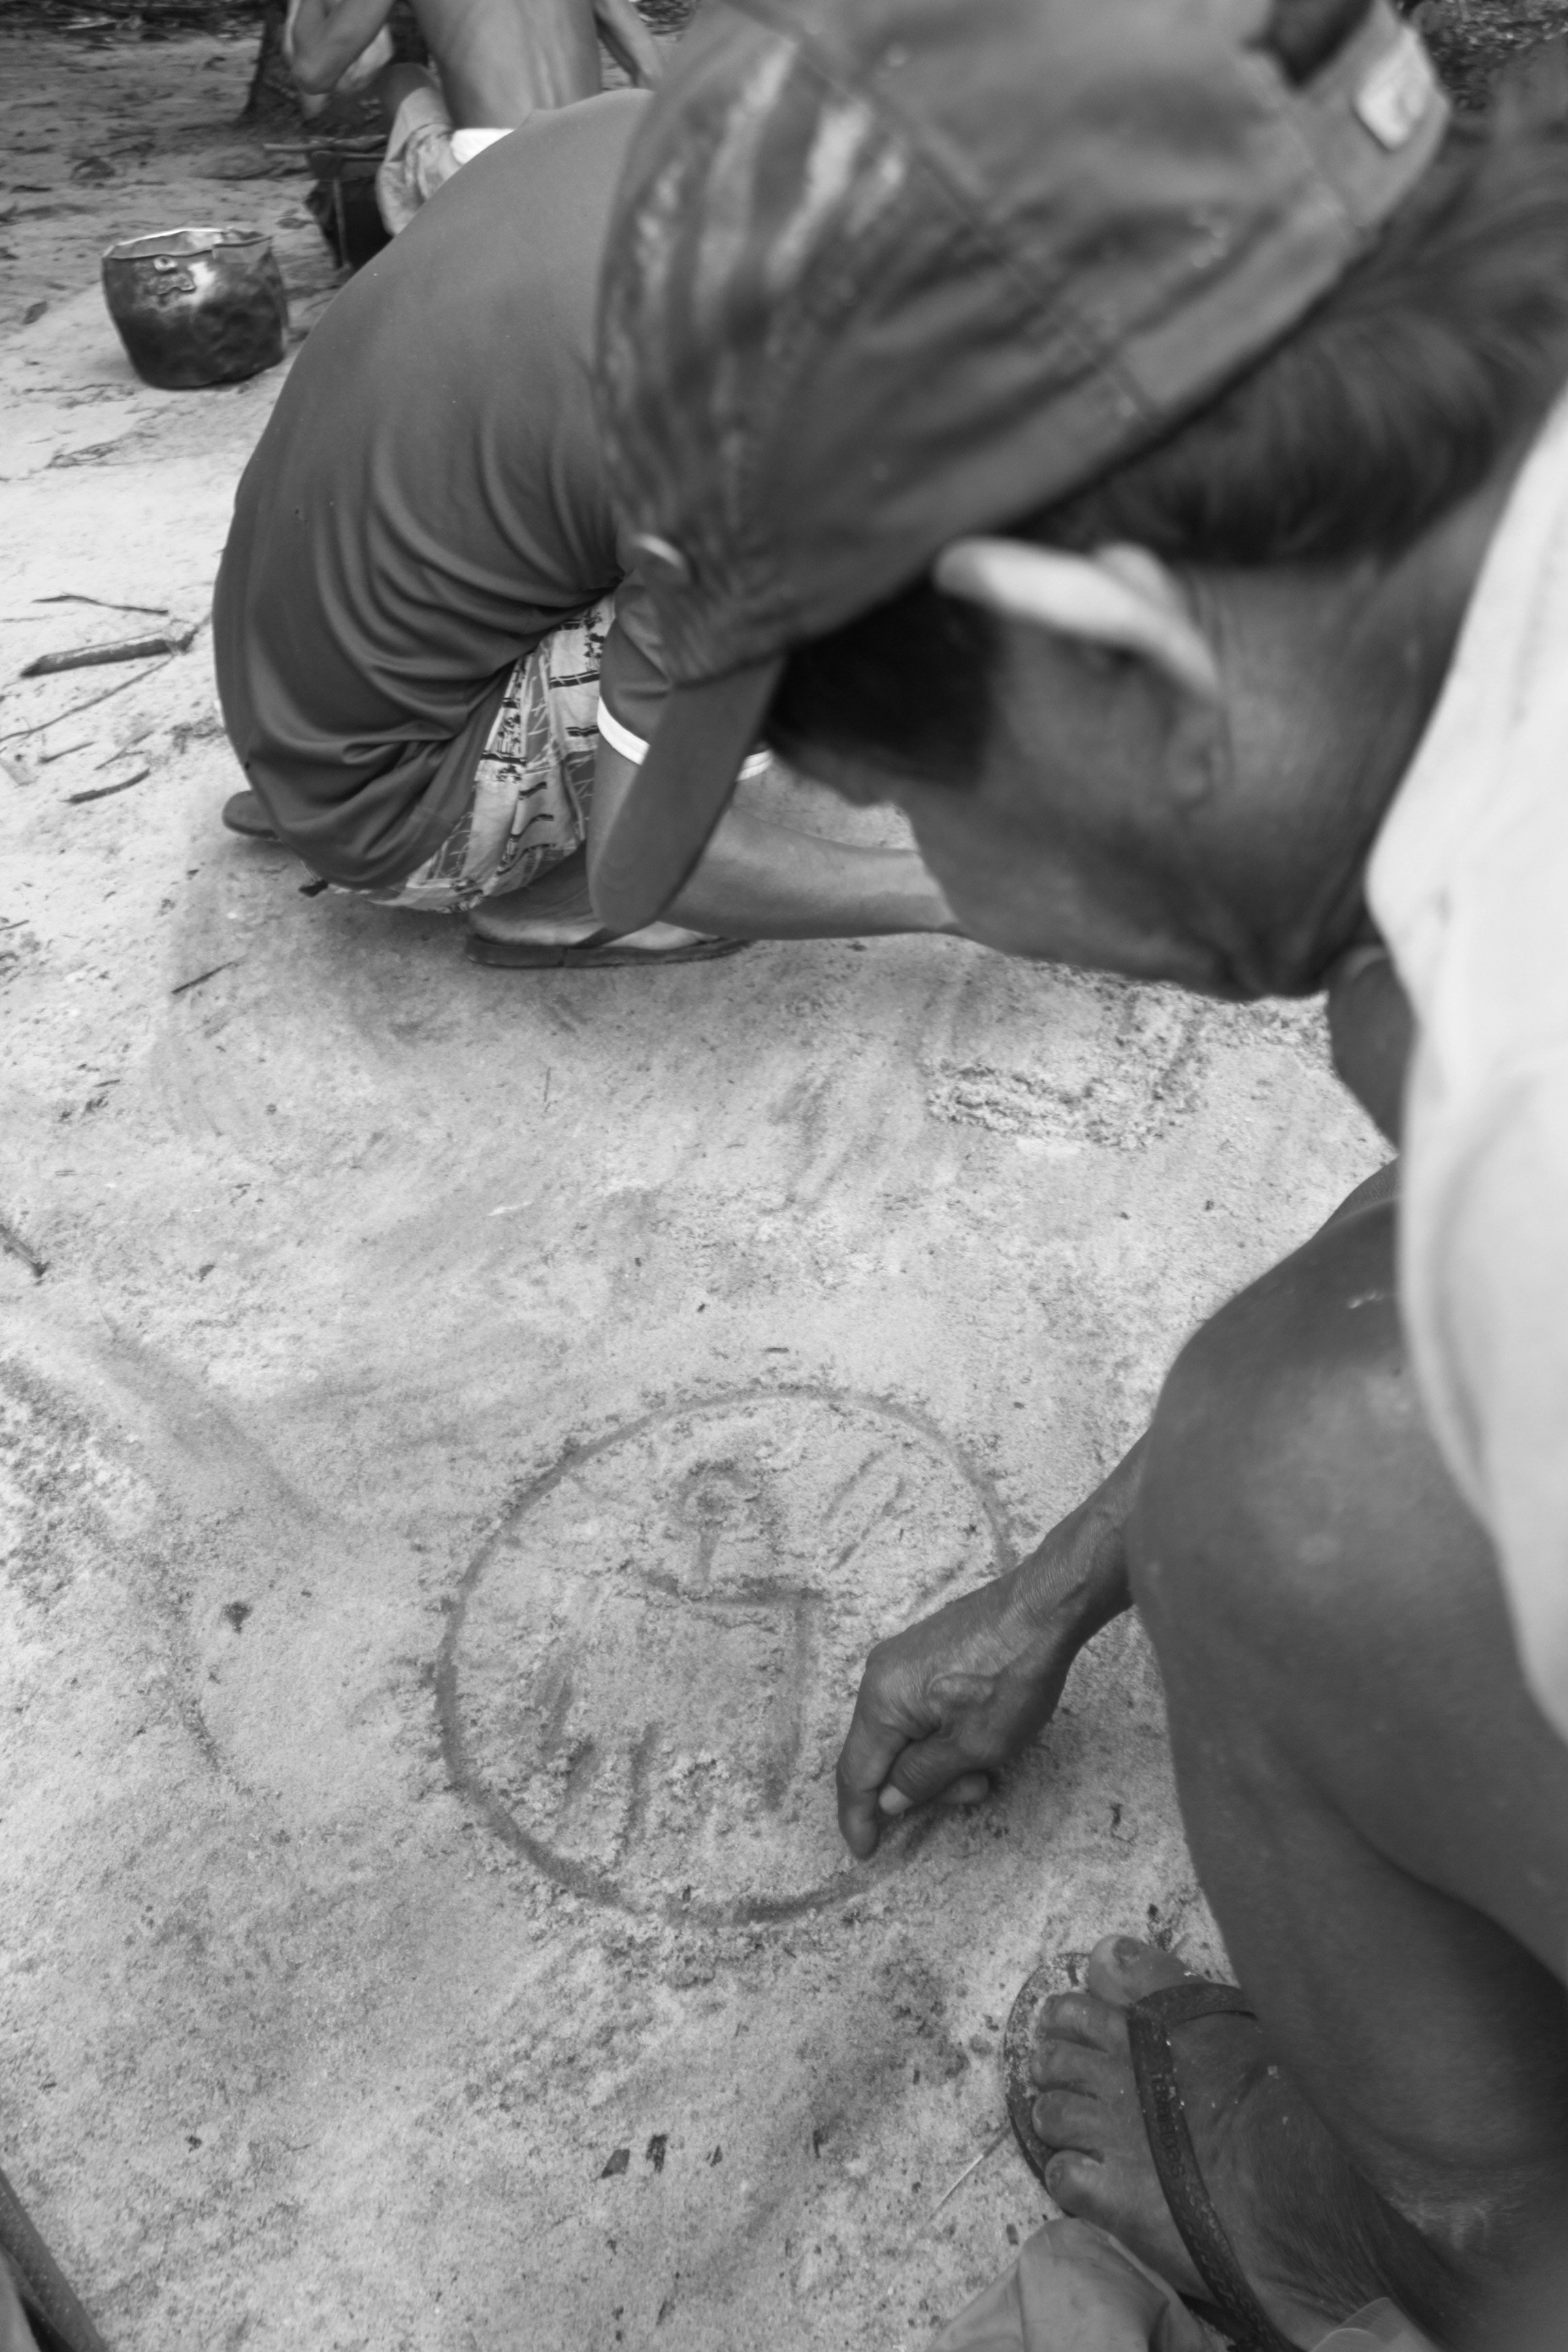
\includegraphics[width=\textwidth]{./img/012}
%\caption{Ponciano mostra o cercar (foto: Danilo P. Ramos, 2012)}
%\end{figure}

% Verificar tabela.
% \begin{figure}[b]
% \centering
% 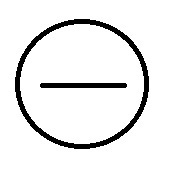
\includegraphics[width=0.2\textwidth]{./img/013}
% \caption{Grafismo do ato de cercar.}
% \end{figure}

Num encontro noturno, pedi a Ponciano e Samuel para me explicarem como
se dava a ação xamânica do cercar durante a execução de encantamentos.
Ponciano voltou"-se para o chão e, com o dedo, começou a desenhar na
areia. Seus traços delinearam um círculo no interior do qual estava uma
pessoa sentada em um banco.\footnote{Por inúmeras vezes, vi os senhores
  hup, ao contarem um encantamento, voltarem"-se para o chão e traçarem
  círculos ou contornos semelhantes. A repetição desses padrões parece
  explicitar a existência de certos grafismos que acompanham a palavra
  xamânica nessas conversas entre mentores e aprendizes.} A postura é
denominada \textit{ɨ̗b' kä̖dä̖t}, ``estar sentado no banco da vida'', ou \textit{pud"-dë̖h
kä̖dä̖t}, ``estar sentado no banco de leite''. Ainda que não se esteja
sentado em um banco de sorva, a postura acocorada ou sentada no chão com
o tronco curvado para frente e as pernas contraídas é igualmente
denominada \textit{banco da vida}. Com a postura corporal, a parte inferior
das costas e as nádegas formam um banco, presente na anatomia humana
desde que o feto se forma na barriga.

Num sentido parecido, o benzedor deve estar deitado dentro de uma \textit{rede
de leite} para viajar até o lago e retornar. Como uma canoa, a rede
torna"-se um veículo de navegação pelo Rio de Leite, \textit{Pu̖d"-Dëh}. Um
pedaço de tabaco sustenta a rede pendurada e aberta para que o benzedor
se movimente deitado. É esse pedaço de tabaco que \textit{cerca} a rede,
ocultando o xamã"-soprador das vistas da Gente"-Cobra para que faça uma
viagem segura durante o trajeto. Enquanto traduzíamos o \textsc{b2},
Samuel deu essa explicação sobre a locomoção do benzedor e fez um
desenho.\index{ac@\textsc{b}2\quad \textit{Hũ̖t bi'i̖d}\break Benzimento do tabaco}

% Verificar tabela.
% \begin{figure}[b]
% \centering
% 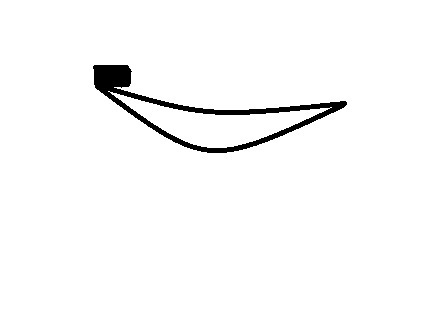
\includegraphics[width=.2\textwidth]{./img/rede_de_leite.jpg}
% \caption{Rede de leite e pedaço de tabaco.}
% \end{figure}

O leite torna"-se a substância comum com a qual são feitos o banco, a
rede, o sopro vital, o pensamento e o lago evidenciando a continuidade
entre as posturas, o corpo, a paisagem e objetos. A fumaça e o pedaço de
tabaco delimitam os contornos e a sustentação para que os alinhamentos
corporais do sentar e do deitar possam se dar com segurança e propiciar
a mobilidade e a agência necessárias. \textit{Sentada em seu banco de leite}
e \textit{deitada em sua rede de leite}, a pessoa alinha seu corpo a partir
de posturas de vida que precisam, elas mesmas, ser protegidas. O círculo
é o envoltório criado pelo gesto de cercar com o qual o benzedor produz
um pari. \textit{Be' ta'yɨ'ɨh}, o ``pari cerca'', diz"-se. O pedaço de tabaco,
sustentando, dá forma à rede e envolve a pessoa"-sopro, cerca"-a ao longo
do percurso de navegação pelo Rio de Leite. Se um Lago de Leite se forma
diante dos senhores sentados em roda, na areia, no centro da roda,
Ponciano desenhava uma pessoa sentada em seu banco de leite e cercada
pelo círculo de fumaça. Sentados em seus bancos, os benzedores
cercavam"-se a si mesmos e ao Lago de Leite com a fumaça de seus
cigarros, pari para envolver a vida e proteger a todos. Com o
\textit{benzimento do tabaco}, o pai de Mandu cercava"-o enquanto ele estava
deitado, sonhando em sua rede.

O Lago de Leite pode ser visto como uma paisagem que represa, que cerca
os princípios vitais, para que a vida possa ser renovada. Tornando"-o
presente diante de si durante a roda, os participantes estão cercando o
entorno a partir dos princípios vitais das águas do lago (leite e
água"-pura), das casas ancestrais às suas margens e dos ornamentos
necessários às danças e rituais (\textsc{b2})\index{ac@\textsc{b}2\quad \textit{Hũ̖t bi'i̖d}\break Benzimento do tabaco}. Enquanto paisagem, o Lago
de Leite é a forma como os Hupd'äh experienciam e reconhecem os
contornos por meio de relações criadas nas atividades práticas das
rodas. Os paris configuram os contornos no curso da atividade pesqueira.
A fumaça, nos atos de benzimento. Creio que a diferenciação que Ingold
faz das cifras e chaves (\emph{clues}) seja interessante para entender
melhor esses sentidos da paisagem do Lago de Leite.

Menos um código e mais uma chave, um indício, um vestígio, um campo de
rastros, a paisagem do Lago de Leite parece guiar o benzedor através de
sentidos desse centro do mundo que se encontram imanentes aos afazeres
diários. As rodas de coca e o Lago de Leite mostram"-se como centros de
atividade progenerativa que situam as pessoas no mundo, numa paisagem
nodal onde as trilhas e as linhas dos movimentos de cada um se cruzam
para formar um campo de percepção e ação. Comendo a coca e postando"-se
às margens do Lago de Leite, os senhores hup nutrem"-se com substâncias e
palavras, crescem e fazem crescer, ao mesmo tempo em que são nutridos
pelos ancestrais. Sentando"-se às rodas, as pessoas passam por linhas de
movimento e troca de substâncias com os presentes, os ancestrais e
demais seres.

Assim, tanto a expulsão do cachorro quanto o desenho do cercar mostram
os limites e contornos desse ambiente protegido para que os senhores se
alinhem corporalmente e, assumindo suas posturas de vida, façam surgir e
possam proteger o Lago de Leite. Revelam"-se os múltiplos estratos da
experiência numa forma unificada, numa paisagem que orienta e abre o
mundo para uma percepção melhor e mais aprofundada. Com a fumaça dos
cigarros os senhores hup cercam a paisagem e a vida, delineando os
contornos dos círculos de coca e fumaça a partir de suas viagens.

\section{Duas viagens}\label{duas-viagens}

Em 4 de março de 2012, a partir de um desenho de Samuel em meu caderno
durante a roda de coca, Miguel foi apontando as casas próximas ao Lago
de Leite. Disse que nos \textit{pë̗' bi'i̖d}, ``benzimento de cura'', é preciso
viajar até o Lago de Leite. Banha"-se a pessoa e seu \textit{hã̗wäg} com as águas
do lago para trocá"-los, \textit{hikad ni̗}, ``transformá"-los''. Deve"-se
parar diante de cada casa, entrar e mostrá"-la à pessoa, para que esta
veja e aprenda a história dos antigos. O percurso torna"-se um caminho ao
longo do qual a pessoa vai sendo socializada ou ressocializada na
paisagem, nas histórias, nas substâncias e ornamentos essenciais para a
fabricação do ser hup. Nesse sentido, em que medida seria possível
pensar a viagem à Serra Grande como uma viagem ao Lago de Leite?

Um dos principais objetivos durante a viagem à Serra Grande era o de
subir o morro e banhar"-se nas águas dos lagos para refazer o corpo,
endurecendo a pele e os ossos para que \textit{todos fossem jovens até a
morte}. O lago é dividido em uma metade masculina e outra metade
feminina. Para banhar"-se a pessoa acocora"-se, encosta suavemente a palma
da mão no centro do lago e, em seguida, passa a mão umedecida no peito,
morada do sopro vital, e depois nos braços. No alto do morro, Lucas
gritou como se estivesse chamando a humanidade (\textsc{m2}) e deixou um
cigarro para os ancestrais no lago.\index{11@\textsc{m}2\quad O grito de \textit{K'e̖g Tẽh}}

%\begin{figure}
%\centering
%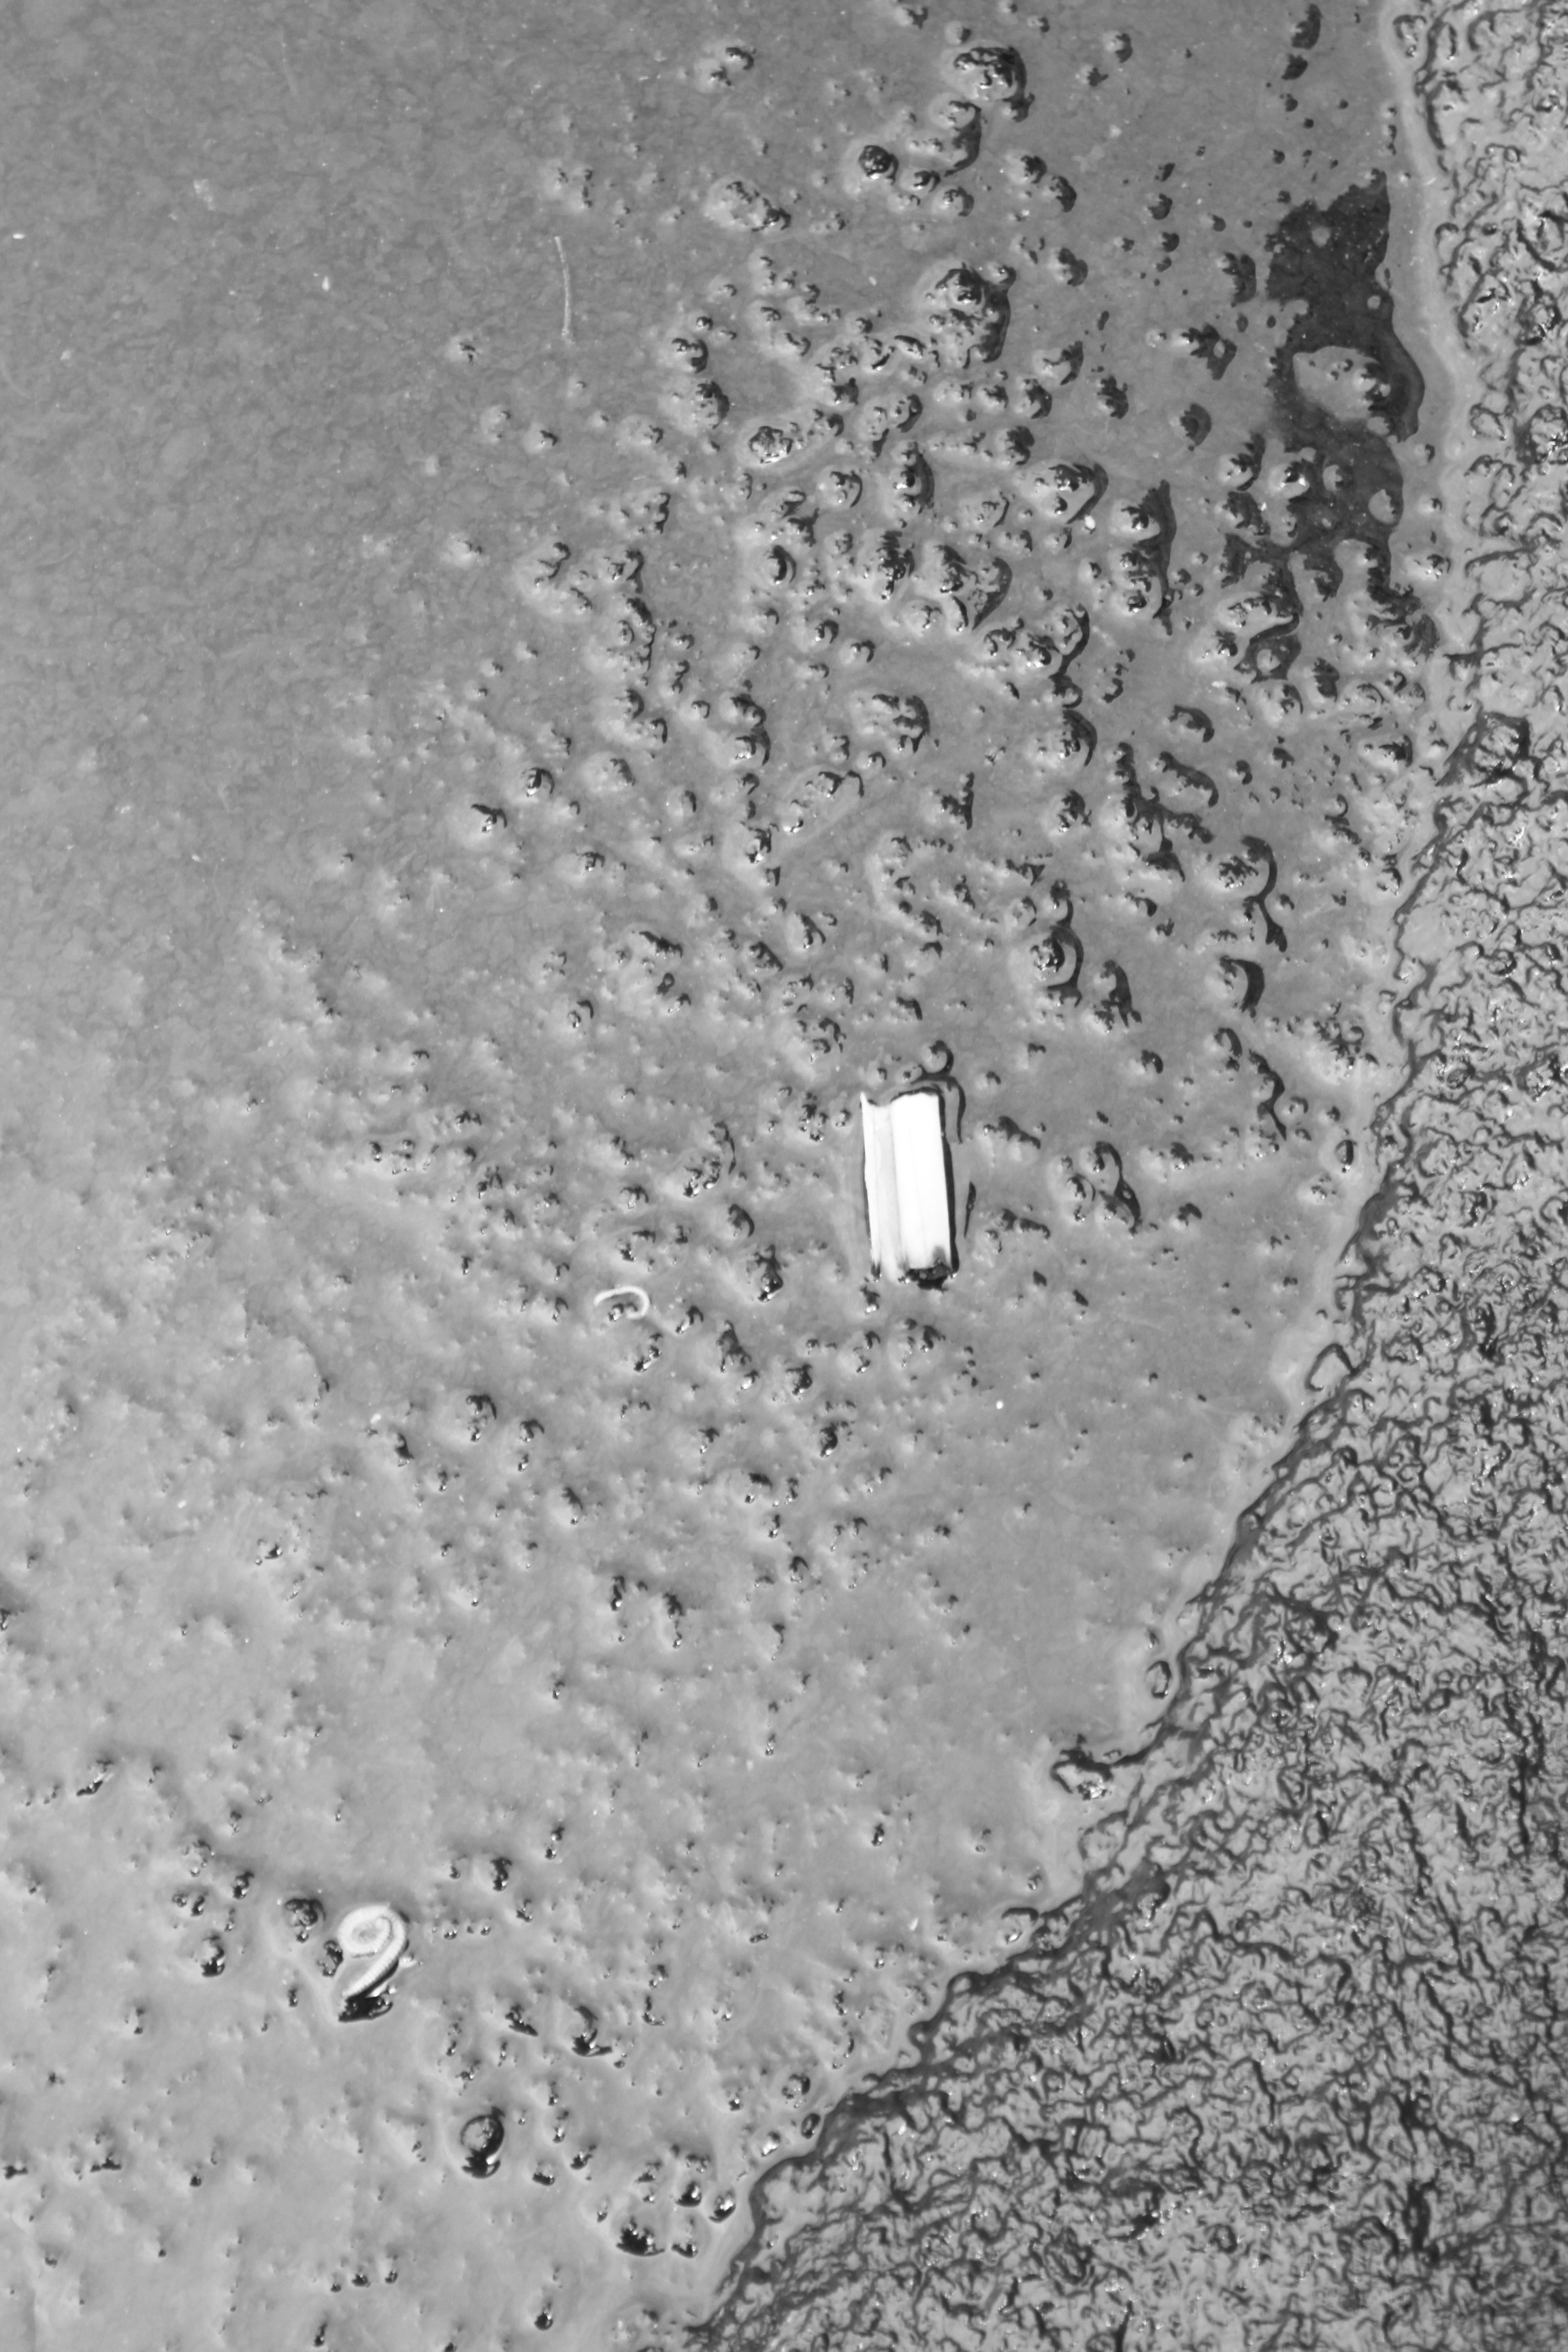
\includegraphics[width=\textwidth]{./img/015}
%\caption{Cigarro no lago (foto: Danilo P. Ramos, 2012)}
%\end{figure}

Como já foi assinalado, no alto da serra, um processo de condensações
rituais situa"-se através do complexo jogo de identificações com os
ancestrais que toma curso pelos gestos dos viajantes, pela manipulação
dos elementos presentes e pelas suas posturas corporais. Nessa casa do
ancestral \textit{Sokw'ät ĩh}, deixar o cigarro no lago é um gesto que se
aproxima da troca do tabaco com os ancestrais realizada pelo benzedor
(\textsc{b2})\index{ac@\textsc{b}2\quad \textit{Hũ̖t bi'i̖d}\break Benzimento do tabaco} ou de uma inversão de papéis, já que é um jovem, um filho
quem está dando cigarro aos antepassados. Como pode ser percebido na
foto, o cigarro é deixado na metade masculina do lago, algo que remete à
reciprocidade agnática e à possibilidade de entrelaçamento das linhas de
vida do jovem e dos ancestrais num modo próximo à comunicação
transversal de \textsc{s1}.\index{ba@\textsc{s}1\quad O pai conta em sonho}

\index{ab@\textsc{b}1\quad \textit{Pũ'ũ̖k bi'i̖d}\break Benzimento da coca}
Tirar o \textit{hã̗wäg} e o tabaco das quatro casas aponta para a associação
fundamental entre o princípio vital e essa substância. Com \textsc{b1}
foi possível entender que banhando o \textit{hã̗wäg}, o xamã purifica e renova a
porção líquida do sopro vital com a água pura do ramo de coca. Como
ressaltou Samuel acima, o sopro vital é composto por água"-pura, leite e
sopro. Banhando a pessoa com a água do Lago de Leite, composta também
por leite e água"-pura, o benzedor troca e regenera esses elementos
vitais. Ele fuma o tabaco em seu banco de leite para criar um pari e
cercar o \textit{hã̗wäg}. Na viagem à Serra Grande, o banho no lago da serra
purificava e renovava o \textit{hã̗wäg} ao mesmo tempo que tornava pele e ossos
estruturas duras que, como um pari de fumaça, cercavam nossos sopros
vitais.

Numa festa de caxiri, Samuel sentou"-se ao meu lado e contou que a aldeia
não estava bem cercada. Por isso, as pessoas das outras vilas teriam
brigado na noite anterior. A comunidade de \textit{Ta̗t"-Dëh} é dividida em
\textit{kopot} ou \textit{potan duy d'äh}, respectivamente ``agrupamentos'',
``vilas'', sendo quatro no total. Em mesmo número que as Casas
Ancestrais, esses \textit{kopot} estão dispostos como se estivessem às margens
de um Lago de Leite no centro. Dos diferentes \textit{kopot}, os benzedores
fazem sopros para cercar o lago e proteger a aldeia de doenças. Cercam
também a maloca para que não haja briga durante as festas. ``Uma hora
são os \textit{Sokw'ä̗t} que estão segurando, outra são os Dâw, outra os \textit{Ɨ̖h Noh
Te̖͂h}. Eles cercam para não ter doença'', disse Samuel. Quando pessoas
começam a brigar, adoecer ou morrer, é preciso que um xamã de outro clã
faça o encantamento novamente, pois aquele que foi feito começa a
demonstrar sinais de fraqueza. Esse encantamento denomina"-se \textit{haya̗m
bi'i̖d}, ``benzimento da aldeia'', e é realizado principalmente com breu.
Em \textsc{b2}, Ponciano menciona que, como a fumaça do cigarro, a
``fumaça do breu é pari para dentro do corpo''.
\index{ac@\textsc{b}2\quad \textit{Hũ̖t bi'i̖d}\break Benzimento do tabaco}

Para as ações xamânicas que visam cercar casas, famílias ou aldeias,
utiliza"-se o ``breu'', \textit{wõ̖h}, por sua fumaça ser mais densa e escura que
a do cigarro. Além disso, uma vez aceso, o breu mantém sua brasa por
muito mais tempo, o que permite ao benzedor \textit{fumaçar} o ambiente de
modo mais completo. Praticamente todas as casas possuem pedaços de breu,
que são o estado sólido de uma resina extraída a partir das árvores
\textit{wõ̖h"-tëg}.\footnote{\textit{wõ̖h"-tëg}, ``breu'', \emph{Protium sp.}, nome dado a
  várias árvores da família das burseráceas. Cf. Ramirez (2006).} Essas
árvores crescem principalmente em \textit{áreas pantanosas}, \textit{b'o̗k}, que
ficam a certa distância das aldeias, na floresta. É durante as incursões
à caça, pesca ou coleta que as pessoas sangram essas árvores para
recolherem a seiva que escorre e, posteriormente, preparar os pedaços de
breu para as ações xamânicas. O breu pode ser usado também no reparo das
canoas, na pintura de objetos (cuias, adornos), e na fabricação de
instrumentos musicais.

%\begin{figure}
%\centering
%
\includegraphics[width=\textwidth]{./img/016}
%\caption{Aldeia cercada (foto: Danilo P. Ramos, 2012)}
%\end{figure}

Como o gesto de \textit{segurar o cigarro}, central para a aliança e para a
continuidade da vida pela prática sexual, os benzedores de diferentes
clãs \textit{seguram a fumaça} que cerca a comunidade e protege o Lago de
Leite, progenerando a vida a partir do centro, o ponto nodal das vidas e
ações dos habitantes. No desenho que Samuel fez na areia, os traços
mostram um grupo de pessoas sendo envolvidas por uma estrutura que as
contém, ao mesmo tempo em que a linha superior se apresenta menor que a
inferior. Também não há uma linha lateral direita. Fixo no leito do rio
ou nas margens arenosas do igarapé, o pari impede a passagem do peixe,
mas mantém"-se aberto pela frente. Da mesma forma, o lago represa a
partir de seu fundo e de suas margens, mas mantém"-se aberto em sua
superfície.

Entendo que a incompletude desse envoltório se deva justamente ao fato
de nenhum grupo ter a habilidade para cercar a totalidade da vida
coletiva. Como o cigarro, que é passado nos Dabucuris, e a coca, que
circula nas rodas, o pari de fumaça vai sendo traçado pelo benzedor de
um dado clã para envolver e proteger a comunidade. À medida que seu
envoltório vai perdendo a força, os seres malfazejos vão conseguindo ver
as pessoas, e, consequentemente, começam a ocorrer doenças e brigas.
Percebendo o enfraquecimento da barreira que sustenta, o xamã passa a
ação ao seguinte, um benzedor de outro clã. Esse, por sua vez, assume a
tarefa e, a partir de seus saberes e habilidades, retoma o movimento de
cercar a aldeia, complementando a agência xamânica de seu predecessor.
Recebendo os poderes e escondendo"-os atrás de si, aprendendo
encantamentos nas rodas e nos sonhos, os saberes de cada grupo
magnificam"-nos diferencialmente e fazem da alternância na ação de
\textit{segurar a fumaça} um processo vital e nunca completo. Creio que essa
ação de cercar a aldeia se dê como um afazer no sentido de Ingold, um
\emph{taskscape}, uma atividade prática executada por um
\emph{agente"-no"-ambiente} em meio a suas ocupações diárias. Numa forma
de atuação mútua e coletiva, as ações xamânicas dos benzedores se dão
conjunta e alternadamente. Sempre cercada, a aldeia nunca está protegida
por completo.

A morfologia da aldeia, tida como a disposição das casas em torno do
Lago de Leite, ajuda a entender a presença imanente da paisagem da origem
criada e recriada no curso do processo vital e da habitação. O \textit{mundo
em miniatura} revelado pela \emph{vista} do alto da Serra Grande
permite agora entender melhor a perspectiva minimalista que leva à
admiração e ao sorriso dos viajantes. O lago diante dos viajantes,
pequeno como uma poça, delineia"-se proporcional em sua forma e tamanho
às serras, Casas"-Ancestrais minúsculas que surgem ao longe, nos cantos
do mundo. Com a vista do topo, os viajantes percebem o aspecto
pluridimensional dos seres, das coisas e do mundo. A paisagem da criação
emerge em sua aura, aparição única de algo distante, o que permite à
pessoa experienciar a existência numa identificação sensorial extrema
com os ancestrais à beira do Lago de Leite.

\index{11@\textsc{m}2\quad O grito de \textit{K'e̖g Tẽh}}
Os gestos de \textit{deixar o cigarro no lago} e \textit{chamar a humanidade}
(\textsc{m2}) apontam para a força da identificação vivida através da
totalidade do ser do viajante a partir de seu corpo, de sua percepção e
de sua ação. Da mesma forma que há uma reconfiguração da pessoa a partir
do sopro (ar) para o deslocamento pelo cosmos, a \textit{fumaça do tabaco é
pari para dentro}, pois cerca o sopro vital, envolve com cascas duras o
corpo. No Lago de Leite, é preciso reunir simultaneamente o sopro vital
e o tabaco para que a pessoa esteja protegida desde esse momento de
regeneração. Fumaça e pari, o tabaco consegue, ao mesmo tempo, envolver
os elementos líquidos e aéreos da pessoa hup, possibilitando e renovando
a vida. O tabaco nas margens cerca o Lago de Leite. Os senhores fumando
cercam a roda de coca. A fumaça no corpo cerca o \textit{hã̗wäg}. Começa"-se a
entender um pouco a analogia entre a pessoa hup e a paisagem do Lago de
Leite.

À luz do comentário de Samuel, creio poder dizer que, depois de nossa
caminhada, enquanto nos banhávamos no alto da serra, um Lago de Leite
tenha igualmente surgido para que nós, como nos encantamentos,
regenerássemos a vida. Mas o banho na serra traz doença e morte se for
tomado apenas uma vez, por isso deve haver um retorno para que o
rejuvenescimento se torne efetivo. Suponho que o risco da viagem única
diga respeito ao perigo da analogia entre os viajantes e os mortos. Como
dito acima, o \textit{hã̗wäg} viaja para a serra, ascende ao topo e depois parte
para o céu, para a casa de \textit{K'e̖g Tẽh} (\textsc{m6})\index{15@\textsc{m}6\quad O caminho dos mortos}. O \textit{b'atɨ̖b'} viaja
para o subterrâneo. A separação definitiva dos princípios vitais atesta
a morte como um \textit{não retorno} e uma \textit{não junção} desses princípios
vitais no corpo. Já os xamãs"-sopradores, preparando o corpo, comendo
coca, fumando e banhando"-se vão e retornam, encontram"-se com os
ancestrais, trocam com eles, conversam, e voltam a seus corpos, a seus
bancos, a suas casas, a suas redes. Como nas perigosas identificações com
a \textit{lagarta que oferece caarpi} (\textsc{b1}) e o \textit{bicho"-de"-pé que,
comendo coca, devora o \emph{hã̗wäg}}, \textit{viajar como os mortos} talvez gere
o perigo de partilhar com eles seus destinos e não retornar da viagem.
\index{ab@\textsc{b}1\quad \textit{Pũ'ũ̖k bi'i̖d}\break Benzimento da coca}

Na segunda viagem, o andarilho está pronto para beber a água do lago e
sonhar como quando se bebe \textit{caarpi}. Isso evidencia a dimensão de
iniciação xamânica do percurso, que se completa quando o andarilho
consegue bebe a água do lago dos ancestrais, aproximando"-se deles para
aprender encantamentos, mas, ao mesmo tempo, consegue retornar. Acordar
depois de encontrar o pai em sonho é uma habilidade que permite lembrar
para benzer, para contar (\textsc{s1})\index{ba@\textsc{s}1\quad O pai conta em sonho}, como fazem os ancestrais em
\textsc{m13}\index{22@\textsc{m}13\quad A dádiva da coca e do tabaco} que fumam e comem coca para \textit{ver e contar}. Ao voltar do Lago de Leite, o xamã"-soprador faz o sopro vital ficar em pé novamente
dentro do corpo do doente, fora da rede, desperto (\textsc{b2})\index{ac@\textsc{b}2\quad \textit{Hũ̖t bi'i̖d}\break Benzimento do tabaco}. Num
dado momento de \textsc{b2}, o benzedor diz: ``para cá eu vou
chegando'', expressão que explicita a viagem xamânica realizada durante
o ato de benzer e a importância do deslocamento e do retorno. Manejando
o tabaco, o sopro, as palavras e as posturas corporais como potências
primordiais, os senhores hup viajam, movimentam"-se, agem, para
comunicar"-se e interagir com esses Outros. O modo como se dá essa forma
de mobilidade, e não apenas a comunicação que ela proporciona, é
fundamental para entender a agência xamânica suscitada pelas rodas de
coca.\footnote{Refiro"-me a certa tendência das análises sobre o xamanismo
  ameríndio de, ao abordar as \textit{viagens xamânicas}, darem ênfase,
  sobretudo, às dimensões comunicativas e linguísticas dos encontros com
  Mestres, por exemplo, e pouca relevância aos processos de
  transformação, gestos e movimentos que ocorrem ao longo dos
  deslocamentos pelo cosmos.}

A habilidade de ir e voltar adquirida na caminhada à Serra Grande é a
mesma de fazer o percurso dos mortos, na totalidade de sua pessoa,
dominando os processos de transformação que envolvem a reconfiguração da
pessoa e sua metamorfose. Esse também é um processo de socialização
correspondente à viagem ao Lago de Leite, pois o caminhante passa pelas
\textit{moradas antigas}, pelas \textit{moradas das onças}, da \textit{Dö̗h A̗͂y}, até
chegar à morada do \textit{Sokw'ät ĩh}, ancestral hup dono da serra.

Conversando com Mandu sobre nossa viagem à Serra Grande discutíamos como
tinha sido difícil e demorado o percurso. Ele então disse que havia duas
formas de viajar e de movimentar"-se: \textit{sa̗pa̗t}, como
``pessoa"-corporificada'', e \textit{hã̗wäg ha̗m}, como ``pessoa"-sopro'' (sopro
vital que vai). Comentava, rindo, que a viagem pelo caminho, como
pessoa"-corporificada, demora muito e é muito difícil. Já a viagem em
benzimento ou sonho, com o deslocamento como pessoa"-sopro, é rápida:
\textit{não demora, chega logo}. Nos encontros noturnos, o Lago de Leite
forma"-se diante dos benzedores sentados em círculo e fumando tabaco,
deslocando"-se como pessoa"-sopro à paisagem da criação para banhar,
tirar, concentrar e regenerar. Simetricamente, caminhando rumo à serra,
viajávamos como pessoas corporificadas rumo a um Lago de Leite para,
como fazem os benzedores, nos banharmos e regenerarmos a vida. Chaumeil
diferencia duas formas de viagem que ocorrem durante o processo de
iniciação dos xamãs yagua,

\begin{quote}
O xamã é por definição aquele que cruza os limites. Embora a viagem
possa apresentar poucos atrativos ao viajante simples, ela se revela
fonte de inspiração e de aprendizado para o xamã. De meu ponto de vista,
é necessário considerar a imagem do xamã fora do meio familiar, e mesmo
fora do meio tradicional, como uma transposição, sobre o plano material,
da \textit{viagem da alma}: ambos experimentam, em níveis diferentes, a mesma
vontade de ultrapassar os limites categoriais e mesmo os limites de si
mesmo.\footnote{1983, p.\,102.}
\end{quote}

Essa oposição entre mobilidade espiritual e material também é utilizada
por Reid para compreender as viagens oníricas e xamânicas como a
\textit{liberação da alma do corpo} num processo que possibilita um maior
conhecimento do mundo não material. Não creio que a diferenciação
estabelecida por Mandu diga respeito a uma oposição entre uma \textit{viagem
da alma} e uma \textit{viagem material} que faça transpor os movimentos
etéreos sobre um plano material, ou que liberte a alma para o
conhecimento do mundo não material. Para além das oposições
material/\,imaterial, continente/\,conteúdo, parte/\,todo que informam essas
visões, creio que andando pelos caminhos ou navegando pelo Rio de Leite
os viajantes assumem regimes distintos de corporalidade, perfazem"-se
como pessoas"-corporificadas ou pessoas"-sopro a partir de seus movimentos
que os permitem concentrar em si potências de intensidades diferenciais
de acordo com os alinhamentos e ações postos em curso.

Calçando suas botas, descrevendo seus passos, abrindo a mata com os
golpes de terçado, escalando os morros, os viajantes projetam"-se,
lançam"-se num contínuo de interação com árvores, rochas, solos, animais
e seres diversos a partir da reconfiguração de si como
pessoas"-corporificadas que vencem inúmeros obstáculos para agir no
\emph{entrecurso} de perspectivas, paisagens, percepções e
sensibilidades. De modo diferente, a desconstrução e reconfiguração que
marca o devir pessoa"-sopro parece convergir para si potências intensas
de velocidade, roupas"-cósmicas, instrumentos de vida e substâncias que
permitem fluir com rapidez entre o aqui e o lá, entre os pontos de
vista, entre posições em campos relacionais, entre as moradas e corpos
de diversos seres.

\index{ba@\textsc{s}1\quad O pai conta em sonho}
Como diz Mandu (\textsc{s1}), benzer e sonhar, \textit{hã̗wäg ha̗m}, são
``trabalhos de médico'', \textit{yõ̖h d'äh bɨ̗' ey ten yɨ̗'}. Ambos são ``árduos''
e, ao mesmo tempo, formas rápidas e menos cansativas de chegar à Serra
Grande, ao contrário da viagem pelo caminho, \textit{sa̗pat}. A \emph{viagem
como pessoa"-sopro} e a \emph{viagem como pessoa"-corporificada}
mostram"-se duas formas de mobilidade que articulam campos relacionais
pelos movimentos, posicionamentos e ações do viajante. Esse ponto de
vista permite rever a oposição de Reid, na qual o \textit{bɨ̗'ɨ̗y}, ``trabalho'',
seria realizado na aldeia como uma atividade árdua e de pouca
mobilidade, enquanto o ``passeio'', ``perambulação'', \textit{k'ët k'ö̗' a̗y}, seria
uma atividade prazerosa, plena de sentido e de alta mobilidade. Sentados
nas rodas, deitados na rede e andando pelos caminhos, os senhores hup
deslocam"-se pelo narrar, pelo benzer, pelo sonhar e pelo vagar, modos de
ação que revelam o envolvimento global com o mundo por meio das
atividades diárias, ``afazeres'', \textit{bɨ̗'}, e ``deslocamentos'', \textit{k'ët k'ö̗'
a̗y}. Essa retradução dos termos talvez ajude a ver os viajantes hup no
contínuo movimento de suas existências. Substâncias fundamentais para o
convívio e para a agência xamânica, o tabaco e a coca mostram"-se não
mais os \textit{objetos do desejo} de caçadores"-especialistas que possuem um
\textit{fraco xamanismo}, mas potências primordiais cujo manejo se dá no
curso das atividades práticas e das situações concretas ao longo da
vida, fundindo o \textit{mundo da aldeia}, o \textit{mundo da floresta} e o
\textit{cosmos} num mesmo mundo vivido que progenera continuamente a pessoa e
a paisagem da criação.

De diferentes formas, endurecer, \textit{tab'a̗'}, e cercar, \textit{ta̗'}, pela fumaça,
casca, paris ou margens do lago conservam e protegem as pessoas hup da
ação dos seres malfazejos. Durante o encontro noturno, sentados em
círculo, os senhores criam diante de si um Lago de Leite semelhante ao
visitado em benzimento, sonho ou nas caminhadas. A percepção dessa
paisagem é um ato de rememoração que se dá não pela projeção, pela
evocação de uma imagem estocada na mente, mas por um ato de engajar"-se
perceptualmente com um ambiente fértil (\emph{pregnant}) de seu passado
através das viagens como pessoa"-corporificada e pessoa"-sopro. Pensando
com Merleau"-Ponty, não há uma projeção coletiva de um quadro do passado,
mas sim o ato mútuo de enveredar no horizonte do passado para ver um
sentido imanente emergir, fazendo convergir as múltiplas perspectivas de
seres, planos"-casa e paisagens para proteger, envolvendo, e curar,
regenerando. Assim, o modo de percepção nas rodas se estabelece muito
próximo à reflexão do filósofo quando mostra que:

\begin{quote}
Perceber não é experimentar um sem"-número de impressões que trariam
consigo recordações capazes de completá"-las, é ver jorrar de uma
constelação de dados um sentido imanente sem o qual nenhum apelo às
recordações seria possível. Recordar"-se não é trazer ao olhar da
consciência um quadro do passado subsistente em si, é enveredar no
horizonte do passado e pouco a pouco desenvolver suas perspectivas
encaixadas, até que as experiências que ele resume como que vividas
novamente em seu lugar temporal.\footnote{2011, p.\,48.}
\end{quote}

O \emph{lago diante de si} e o \emph{lago de destino} envolvem cada
participante na essência da totalidade de suas relações. É através do
movimento corporal da pessoa sentada e viajando pelo cosmos, \textit{hã̗wäg
ha̗m}, ou do percurso da trilha para a Serra Grande, \textit{sa̗pa̗t}, que essa
paisagem é experienciada como um nexo em si, distinto de outros. As
rodas de coca e a viagem à Serra Grande mostram"-se formas de
sociabilidade ritual imersas nos afazeres diários. Sua temporalidade
social não é marcada por enquadramentos (\emph{frames}), mas pela
atenção que as pessoas, no curso de suas atividades necessárias à
habitação, dão a essas \emph{performances}. O ato de caminhar para a
Serra Grande refaz as trilhas e regenera a pessoa através dos banhos. A
viagem xamânica ao Lago de Leite socializa com os atos de mostrar as
casas, os ornamentos, as paisagens.

O cachorro que atravessa o lago torna"-se um elemento indesejado, já que
se está compondo, coletivamente, uma paisagem que situa o espaço"-tempo
do surgimento da humanidade, da dádiva do cigarro, da coca, e da
reciprocidade entre a pessoa hup e seus antepassados através de uma
sequência de ações que pode ser afetada pela presença canina. A
identificação que permite ao benzedor trocar o tabaco e os ornamentos
com os ancestrais das casas (\textsc{b2})\index{ac@\textsc{b}2\quad \textit{Hũ̖t bi'i̖d}\break Benzimento do tabaco} assemelha"-se àquela que
garante o aprendizado de Mandu em sonho com o pai morto (\textsc{s1}) e\index{ba@\textsc{s}1\quad O pai conta em sonho}
à dádiva da coca, do tabaco, para revelar, geração após geração, as histórias
dos antigos (\textsc{m13}). A paisagem do Lago de Leite é o mundo tal
como ele é conhecido por aqueles que existem movendo"-se pelos caminhos
vividos. É o lugar de nascimento e de contínuo renascimento da
humanidade através da palavra, das substâncias, das viagens e dos
círculos de fumaça.\index{22@\textsc{m}13\quad A dádiva da coca e do tabaco}

\part{Círculos e caminhos}\label{segunda-parte---cuxedrulos-e-caminhos}

\chapter{Caminhos abertos}\label{caminhos-abertos}

\setlength{\epigraphwidth}{.60\textwidth}
\begin{epigraphs} 
\qitem{Caminho por uma rua\\
Que passa em muitos países\\
Se não me veem eu vejo\\
E saúdo velhos amigos.}{\textsc{carlos drummond de andrade},\\\textit{Canção amiga}}
\end{epigraphs}

\section{O caminho das nuvens}\label{o-caminho-das-nuvens}

Às vésperas de nossa viagem às serras para pescar e visitar os lugares
sagrados, a chuva insistia em cair. Parecia mais forte a cada dia. No
final da tarde, as tempestades invadiam a aldeia com suas águas, ventos
fortes e relâmpagos que dificultavam a realização das rodas de coca e
adiavam nossa caminhada. Estávamos ainda no \textit{Ya'a̗m"-Sõ̖h"-Dëh}, o
Inverno"-da"-Onça: ``Essa é a última parte, o rabo da onça'',
explicava Ponciano, tranquilizando"-me de que logo realizaríamos nossa
andança. Com a chegada do verão de \textit{Wero"-M'e̗h"-Töd},\footnote{Seguindo a
  tradução de Ramirez (2006), \textit{Wero M'e̖h Töd} seria o Verão do
  Bigodinho, pássaro da família dos fringilídeos que corresponde a uma
  constelação visível nessa época do ano.} os caminhos secariam, as
jararacas buscariam abrigo em suas tocas e poderíamos seguir
tranquilamente.

Foi então que, no dia 7 de março de 2012, uma massa de nuvens negras
formou"-se no céu quando estávamos sentados em roda. Com toda a força de
suas águas e ventos, a tempestade vinha em direção à aldeia. Os
estrondos dos trovões e a claridade dos relâmpagos assustavam a todos.
Ponciano parou de falar. Começou a soprar um cigarro. Os lábios
pronunciavam palavras silenciosas. Num dado momento, acendeu o fumo e se
levantou. Tragou. Fechou sua mão direita e levou"-a para perto da boca.
Os olhos parados nas nuvens negras que se aproximavam. Um sopro vindo do
peito lançou a fumaça para fora do corpo. Ao mesmo tempo, Ponciano
arremessou com força sua mão e seu braço para longe e fez com que a
tempestade rumasse por outro caminho para a \textit{Dëh"-K'et"-Yoh"-Mo̖y}, a
Casa"-da"-Cabeceira.

Depois, o benzedor sentou"-se novamente. Retomou seu lugar à roda. Queria
contar"-me como se realiza esse \textit{dëh bi'i̖d}, ``benzimento da chuva'', que
faz com que as nuvens se afastem para outro caminho no céu e não
despejem suas águas, raios e trovões sobre a aldeia. Sentados em
círculo, comíamos coca, fumávamos e conversávamos num grupo de nove
pessoas.

%\bigskip

\begin{quote}\index{ad@\textsc{b}3\quad \textit{Sõ̖h ta̗' bi'i̖d}\break Benzimento de cercar a chuva, ou o inverno}
\benzimento{3}{\textit{sõ̖h ta̗' bi'i̖d}, «cercar a chuva, ou o inverno»}

Você fala o nome de \textit{Mu'se'}, aquele da bíblia. Você se levanta e abre
os braços como ele fez para abrir o Mar Vermelho. Como ele, você afasta
as águas para as cabeceiras.
\end{quote}

%\bigskip

%\index{ae@\textsc{b}4\quad \textit{Sõ̖h ta̗' bi'i̖d}\break Benzimento de cercar a chuva, ou o inverno}
% \benzimento{4}{\textit{Sõ̖h ta̗' bi'i̖d}, «cercar a chuva, ou o inverno»}

\begin{quote}
\begin{itemize}
\item[1º \textsc{mov}\quad] Lê"-se a tartaruga vermelha e sua canoa. A tartaruga preta e sua canoa. Fala"-se para ela colocar todas as suas coisas em sua casa, dentro de sua canoa, e ir nadando até a cabeceira.
\paragraph{Comentário} Seu nado, o movimento de suas nadadeiras vai separando a água. Como Moisés quando separou as águas. Isso vai cercando a água também. 
\medskip

\item[2º \textsc{mov}\quad] Fala"-se para suas \textit{dëh hup hẽ̖h}, para suas ``coisas'', ``armas da água''. Fala"-se para seu \textit{he̖͂y'"-b'ah}, ``remo'', e para sua \textit{he̖y' b'ah}, sua ``tesoura da origem''. Então, conforme ela vai nadando ela afasta a água da chuva e cerca. 
\end{itemize}
\end{quote}

O fato de Ponciano, \textit{yo'o̗m ĩh}, ``dono'', de \textit{Ta̗t"-Dëh} ter se levantado
no momento em que as nuvens se aproximavam ameaçadoramente ressalta seu
lugar de prestígio político"-ritual e sua competência xamânica. As nuvens
afastaram"-se logo depois que ele realizou o ato de benzimento e recebeu
o olhar de aprovação e reconhecimento de seus companheiros. Em seguida,
sentou"-se e começou a contar"-me os encantamentos. Ele é um dos poucos
que pode ensinar essa prática aos não hup.

Em pé com o corpo voltado para as nuvens que se aproximavam, o velho
Ponciano evocava as ações de Moisés e as das tartarugas. Seus gestos
fizeram com que a fumaça que saía de sua boca fosse lançada em direção
às nuvens. Ao jogar seu braço, fez com que elas rumassem para a
Casa"-da"-Cabeceira. Sobre a relação entre as nuvens e a fumaça do
tabaco no xamanismo desana, Reichel"-Dolmatoff diz que,

\begin{quote}
Há uma reação entre o fumo e a chuva, sendo esta última naturalmente um
elemento fertilizador. Assim como a chuva apaga o fogo, o fumo de tabaco
é uma imitação das nuvens, pode dispersá"-las ou também aglutiná"-las. Por
outro lado, o fumo torna invisível e é, por conseguinte, um elemento de
defesa.\footnote{1986, p.\,183.}
\end{quote}

Como visto no capítulo anterior, os senhores hup fumam para conversar,
ouvir encantamentos e histórias que permitem nutrir e fazer crescer a um
só tempo os filhos e o pensamento. Se a chuva faz crescer as plantações,
ela também apaga o fogo, impede a continuidade das rodas de coca e,
consequentemente, o fluxo das conversas. Na relação que se estabelece
com as nuvens ocorre uma interação entre uma fumaça terrestre e uma
fumaça celeste. O benzedor imitava o nado da tartaruga abrindo os braços
e espalhando o ar à sua frente. Moisés abriu o Mar Vermelho. Estendeu a
mão e Javé fez soprar um vento oriental muito forte que perdurou a noite
inteira e dividiu as águas em duas. Lançando o braço à frente, Ponciano
imitava o ancestral dos brancos. A coluna de nuvens que acompanhava o
\textit{povo de Deus} retirou"-se da frente deles e colocou"-se atrás. Assim, o
\textit{povo de Deus} pôde seguir, atravessando o mar Vermelho com os \textit{pés
enxutos}. Continuaram pelo caminho indicado por Javé, que os levaria ao
Monte Sinai e à Terra Prometida, onde corre leite e mel. Pela manhã,
quando os soldados egípcios atravessavam o mar aberto, Javé fez as
colunas de água desabarem sobre eles, aniquilando"-os completamente.\footnote{\textit{Êxodo}, 3,14; 4,33.}

Para que pudéssemos viajar para os morros e para as Moradas Antigas, o
xamã alterou o rumo das nuvens da tempestade para a cabeceira, fazendo
com que os caminhos alagados secassem. Creio que essas múltiplas
interações com as nuvens, de humanos e quelônios, sejam possíveis a
partir da observação e da imitação, possibilitadas por processos de
educação da atenção desses atores em seus ambientes, tal como Ingold
propõe:\footnote{2000, p.\,37.} ``observar é ter atenção aos movimentos dos
outros; imitar é alinhar essa atenção aos seus próprios movimentos
práticos orientados para o ambiente''.

Nesse sentido, o xamã observa os corpos celestes, as tartarugas e o
profeta. Suas palavras, movimentos corporais e fumaça são gestos que
imitam para interagir com as nuvens e, assim, com \textit{Pe̗͂y Wäd}, o
Trovão. Dias antes, enquanto estávamos reunidos para comer coca, uma
forte tempestade caiu sobre a comunidade. Levamos os banquinhos para
debaixo da casa do forno e lá nos sentamos. Os raios que caíam na mata
próxima à aldeia e os trovões ensurdecedores faziam com que sentíssemos
muito medo. Ponciano e João penduravam"-se nos travessões da casa e davam
pulos a cada vez que ouviam um estrondo. Vicente reclamou: ``Se a
comunidade estivesse bem cercada, o menino Guilherme não teria ficado
doente''. Sua doença fora causada pelos trovões, assim como as doenças
de muitas crianças e adultos. Américo cobria com as mãos as orelhas do
filho. Alertou que o barulho dos trovões entra na orelha, suja a
\textit{b'oto̗k"-mo̖y}, a ``casa"-da"-audição'', e causa dores de cabeça, desmaios e
perda de consciência.

A tempestade e os barulhos ensurdecedores do trovão faziam com que
muitos dos participantes dissessem a seguinte frase: \textit{Pẽ̗y pũ'ũ̗k we̗d
tuy}, ``o Trovão quer comer coca''. Como visto anteriormente, no final
da tarde não são apenas os homens hup que preparam a coca para comê"-la
cerimonialmente. Nas Casas do Céu, da Mata e dos Rios, diversos seres
preparam coca para oferecê"-la a seus cunhados. No caso, se o Trovão quer
comer coca, é porque as Onças, seus cunhados, não estão oferecendo o
alimento a seu dono. Agindo como um \textit{benzimento da aldeia}, o sopro da
fumaça faz com que as nuvens mudem seus rumos e dirijam"-se à cabeceira.
A comunidade é cercada através desse procedimento que, ao afastar a
chuva, impede que a fúria do Trovão atinja a aldeia.

%\begin{figure}
%\centering
%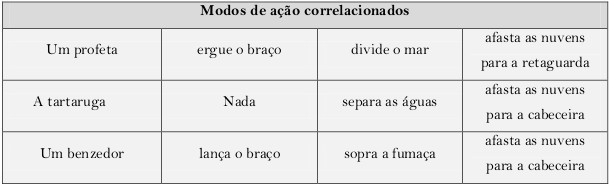
\includegraphics[width=\textwidth]{./img/q3}
%\caption{Quadro comparativo de ações}
%\end{figure}

% Please add the following required packages to your document preamble:
% \usepackage{booktabs}
% \begin{table}[]
% \centering
% \begin{tabular}{@{}cccc@{}}
% \toprule
% \multicolumn{4}{c}{\textbf{Modos de ação correlacionados}} \\ \midrule
% Um profeta & ergue o braço & divide o mar & \begin{tabular}[c]{@{}c@{}}afasta as nuvens\\ para a retaguarda\end{tabular} \\ \midrule
% A tartaruga & nada & separa as águas & \begin{tabular}[c]{@{}c@{}}afasta as nuvens\\ para a cabeceira\end{tabular} \\ \midrule
% Um benzedor & lança o braço & sopra a fumaça & \begin{tabular}[c]{@{}c@{}}afasta as nuvens\\ para a cabeceira\end{tabular} \\ \bottomrule
% \end{tabular}
% \caption{Quadro comparativo de ações}
% \label{my-label}
% \end{table}

%\textbf{Modos de ação correlacionados}\\
\begin{itemize}
\item \textsc{um profeta}\quad, Ergue o braço \rightarrow\, Divide o mar \rightarrow\, Afasta as nuvens para a retaguarda
\item \textsc{a tartaruga}\quad Nada \rightarrow\, Separa as águas \rightarrow\, Afasta as nuvens para a cabeceira
\item \textsc{um benzedor}\quad Lança o braço \rightarrow\, Sopra a fumaça \rightarrow\, Afasta as nuvens para a cabeceira
\end{itemize}

As ações do benzedor, do profeta e da tartaruga geram mudanças num dado
ambiente com o qual se relacionam. De modo muito interessante, a viagem
de Moisés e seu povo rumo à Terra Prometida parece ser uma transformação
da viagem da tartaruga com destino à Casa"-da"-Cabeceira. Soprando essas
agências para o cigarro, o deslocamento da fumaça e o movimento corporal
alteram o destino da tempestade.

\index{ad@\textsc{b}3\quad \textit{Sõ̖h ta̗' bi'i̖d}\break Benzimento de cercar a chuva, ou o inverno}
Pensando com Carneiro da Cunha, \textsc{b3} pode ser tomada como uma
tradução xamânica de \textsc{b4}\index{ae@\textsc{b}4\quad \textit{Sõ̖h ta̗' bi'i̖d}\break Benzimento de cercar a chuva, ou o inverno}, possivelmente elaborada após a
consolidação dos \textit{povoados"-missão} como \textit{Ta̗t"-Dëh} e da participação
das missas, das escolas salesianas, dos batismos que foram situando os
Hupd'äh num processo de evangelização já em curso com outros povos da
região. Como o povo de Israel, eles viajavam para terras distantes, para
longe das cabeceiras, das \textit{Paç"-Mo̖y}, Casas"-de"-Pedra, próximas às
quais seus ancestrais procuraram sempre constituir suas moradas. Como
aponta Reid,

\begin{quote}
A partir desses dados fica claro que, antes de 1890 e até 1950,
virtualmente todos os Hupdʉ viviam nas cabeceiras dos igarapés
tributários aos que ocupam atualmente. Alguns Hupdʉ afirmam que
Salesianos ordenaram que migrassem rio abaixo, ao mesmo tempo em que os
Índios do rio foram ordenados a fazer o mesmo (1930-40). Entretanto,
fica evidente que os Hupdʉ não fizeram isso até o início dos anos de
1940, sendo que a maior parte mudou"-se apenas nos anos de 1950. Os novos
assentamentos estabeleceram"-se entre uma e quatro horas de caminhada com
relação aos grandes rios. Em alguns anos, esses assentamentos mudavam"-se
para áreas das imediações, ao longo do igarapé onde já estavam situados
ou para igarapés próximos. Atualmente, os Hupdʉ estão vivendo
principalmente nas partes rio abaixo dos igarapés tributários aos que
ocupavam previamente.\footnote{1979, p.\,28.}
\end{quote}

De acordo com o antropólogo, antes de 1890 e até 1950 os Hupd'äh viviam
na região das cabeceiras dos igarapés ao longo dos quais se encontram as
aldeias atuais, situadas em áreas mais próximas aos grandes rios.
Entretanto, a violência posta em prática com o \emph{boom} da
borracha (1890 a 1900) e com a atuação dos representantes
governamentais (Manducas)\footnote{Wright comenta que Manuel
  Albuquerque, o ``Manduca'', fora um brasileiro mestiço que ocupou o
  posto de subprefeito de São Gabriel, obtido no auge do \emph{boom} da
  borracha. Com a ajuda dos irmãos, ele controlava o trabalho indígena
  por meio da violência e terror (Wright, 2005, p.\,213).} teria levado
os Tukano a deixarem a área ribeirinha para fixarem"-se em aldeamentos
nas áreas florestais, a algumas horas de caminhada. Segundo Reid, esse
deslocamento populacional tukano levou as comunidades hup a afastarem"-se
para áreas ainda mais próximas às cabeceiras. Como visto, durante a
viagem à Serra Grande, os \textit{espaços da morte} povoam a região trazendo
lembranças dos confrontos e das vítimas. Os representantes
governamentais, os exploradores de borracha e mesmo os Tukano muitas
vezes atacavam as aldeias hup para assassinar e escravizar pessoas.

Tomando os Hupd'äh como \textit{S'u̖g Hup}, ``gente da floresta'', Reid reforça
a ideia de que seriam eles, enquanto Maku, os \textit{primeiros habitantes}
do Uaupés, caçadores"-coletores que constituíam suas aldeias numa vasta
região interfluvial. Enquanto Koch"-Grümberg e Nimuendaju veem a pressão
exercida pelas populações Tukano e Aruaque como o fator que teria levado
ao afastamento dos Maku para as cabeceiras (\textsc{s.e.} para \textsc{n.o.}), Reid retoma
essa hipótese numa chave que considera os não indígenas e os Tukano como
sendo os agentes políticos que forçam os Hupd'äh a migrarem,
refugiando"-se na região montanhosa. Para além dessa visão que oscila
entre a caracterização dessas áreas como refúgios ou repositórios de
recursos econômicos, creio que nossa jornada às cabeceiras possa ajudar
a perceber a importância ritual que faz desses lugares paisagens de vida
fundamentais para a interação dos Hupd'äh com esses Outros.

Nos anos 1940, ocorreu a aproximação dos salesianos, muitas vezes mediada
pelos Tukano. Os missionários balizavam seu \textit{projeto civilizatório} no
aprendizado do português, na moradia em casas nucleares e na conversão
cristã, além de condenarem a ação dos exploradores de borracha. Para
Reid, o fato de os religiosos apresentarem"-se como uma alternativa face
ao terror praticado pelos demais brancos provoca, na década de 1950, a
migração de muitas aldeias para as imediações dos grandes rios e, anos
mais tarde, a consolidação das grandes comunidades, denominadas por
Athias como \textit{povoados"-missão}.

À luz da analogia bíblica, esse movimento migratório para as cabeceiras
assemelha"-se ao Êxodo, uma fuga da perseguição dos soldados egípcios. O
paralelo entre os percursos e os sentidos dos deslocamentos desses
vários agentes dos encantamentos torna"-se interessante para entender o
processo histórico que levou à constituição da grande aldeia de
\textit{Ta̗t"-Dëh}. Retomando \textsc{b3}\index{ad@\textsc{b}3\quad \textit{Sõ̖h ta̗' bi'i̖d}\break Benzimento de cercar a chuva, ou o inverno} e \textsc{b4}\index{ae@\textsc{b}4\quad \textit{Sõ̖h ta̗' bi'i̖d}\break Benzimento de cercar a chuva, ou o inverno}, num caso, os \textit{filhos de
Israel} conseguem fugir dos exércitos egípcios \textit{passando pelo mar com
os pés enxutos} rumo à Terra Prometida (\textit{Êxodo}, 3, 14; 4, 33). No outro,
para que não haja trovões e doenças, para que possamos viajar tranquilos
para os \textit{lugares sagrados} e para que a roda de coca não precise
transferir"-se para o coberto, a fumaça faz as nuvens afastarem"-se. Lê"-se
a tartaruga vermelha e sua casa"-canoa, a tartaruga preta e sua
casa"-canoa. O benzedor faz com que o anfíbio coloque suas armas da
origem na canoa, principalmente sua tesoura, e vá nadando para a
cabeceira do rio. Suas nadadeiras vão separando a água como Moisés
separou o Mar Vermelho. Nadando, ela faz as nuvens e a chuva rumarem
para a Casa"-da"-Cabeceira.

Ao mesmo tempo, nossa viagem seria realizada \textit{sa̗pa̗t}, como
pessoas"-corporificadas, andando pelos caminhos, num percurso semelhante
ao deslocamento \textit{hã̗wägat}, como pessoas"-sopro, que faz os xamãs hup
chegarem às Casas"-de"-Pedra. Surpreendentemente, o Êxodo até o Mar
Vermelho e a migração dos Hupd'äh para as imediações do rio Tiquié são
deslocamentos populacionais que se dão no sentido \textsc{n.o.} para \textsc{s.e.} Na
leitura xamânica hup do texto bíblico, Moisés desloca as nuvens para
trás, para as cabeceiras, distanciando"-as do Mar Vermelho assim como as
nascentes estão distantes do rio Tiquié. No mesmo eixo, a viagem que
faríamos aos lugares sagrados, o percurso da tartaruga em \textsc{b4}\index{ae@\textsc{b}4\quad \textit{Sõ̖h ta̗' bi'i̖d}\break Benzimento de cercar a chuva, ou o inverno} e
o afastamento das nuvens estabelecem"-se no sentido inverso \textsc{s.e.} para
\textsc{n.o.} Caminhando, iríamos abrir as trilhas fechadas pela floresta e pelo
tempo.

Nos dias que se seguiram, não houve mais tempestades e começamos a
preparar nossas coisas para a jornada. Viajaríamos num grupo a ser
formado por rapazes e senhores. Nesses dias de espera, as mães dos
jovens viajantes torraram uma quantidade suficiente de farinha para que
seus filhos não passassem fome no percurso. Ponciano preparou sua flecha
com curare, caso fossemos surpreendidos por uma onça. Todos ajeitaram
seus arcos e seus caniços para a caça e pesca. Nos encontros noturnos e
na festa de caxiri, antes de nossa andança, os dois guias
reorientavam"-se. Discutiam longamente os caminhos e direções com os
outros senhores. Fazia algum tempo que ambos não caminhavam por aquelas
searas onde haviam sido criados.

A vida nas aldeias populosas fez com que cada vez menos pessoas se
deslocassem até as cabeceiras ou às regiões onde antes havia os caminhos
de roça, os trajetos para outras aldeias, as áreas de caça e as
Casas"-de"-Pedra. Os rapazes nunca tinham percorrido aquelas paisagens
distantes e seu fascínio pela empreitada fazia com que todas as noites
viessem à roda de coca para conversar com os mais velhos e prepararem"-se
para a viagem. Nossa jornada aos \textit{lugares sagrados} constituir"-se"-ia
ao mesmo tempo de atos de relembrar dos mentores que visitariam os
lugares onde cresceram e conviveram com seus pais e avós, e de percursos
de observação, ao longo dos quais os jovens conheceriam histórias e
seres através de seus próprios movimentos e ações, e por meio das
indicações e narrativas dos mais velhos.

Para que estivéssemos bem protegidos durante a viagem, além do
\textit{encantamento para afastar a chuva}, Ponciano preparou um cigarro com
o \textit{ti̖wi̖t hamap bi'i̖d ta̗'}, ``benzimento dos caminhos'', para cercar os
viajantes das ações maléficas dos seres que pudéssemos encontrar.



%\section{Caminhos cruzados}

\section{O caminho dos Hupd'äh}\label{o-caminho-dos-hupduxe4h}\label{caminhos-cruzados}

Com a certeza de que não haveria mais chuvas, deixamos a aldeia depois
dos banhos e de nossa refeição matinal. Uns levavam jamaxins às costas,
outros mochilas para carregar as redes, a farinha, os anzóis e algumas
poucas peças de roupa. Éramos sete pessoas, jovens em sua maioria,
guiados por dois senhores, Ponciano e seu irmão menor, José. As serras
que visitaríamos situavam"-se todas nas dimensões territoriais de domínio
dos \textit{Sokw'ät"-Noh"-Köd"-Tẽ̖h}, cujo representante superior vivo é Ponciano.

Todos carregavam seus arcos e flechas nas mãos junto aos caniços para a
pesca. Apenas Ponciano levava uma \textit{mo̖m"-mu̖h}, flecha com a ponta de ferro
munida de curare. Essa era nossa proteção contra as onças ou seres
malfazejos que viessem ao nosso encontro. As pontas das flechas de cada
um dos viajantes variavam a partir de dois padrões. As flechas
específicas para as caças que se movimentam no alto das árvores, como os
macacos e as aves, tinham pontas de madeira estreladas. Já as flechas
para as caças de solo, como pacas, queixadas, tamanduás, tinham finas
pontas de madeira. A passos rápidos, seguíamos pelos caminhos da roça
que se transformavam em \textit{hup ti̖w}, ``caminhos de hup'', estreitos e
traçados sobre as raízes e folhas caídas.

Ainda estávamos numa clareira, próxima às últimas roças da comunidade,
quando todos pararam para descansar. Rindo, os jovens apanharam flores
amarelas de um tipo encontrado nas caatingas e colocaram"-nas em suas
orelhas. Faziam como os antigos, antes de começarem a dançar. De modo
divertido, nossa caminhada para as serras assemelhava"-se a uma dança, a
uma festa que unia a todos no convívio de um percurso desconhecido para
a maior parte dos viajantes. Ponciano acendeu um cigarro. Tragou. Soprou
a fumaça em seu corpo e passou"-o a Ari para que este fizesse o mesmo.
Quando terminou, o rapaz passou adiante o cigarro que circulou de mão em
mão até que todos tivessem soprado a fumaça em seus corpos. O cigarro
tinha sido preparado dias antes com o \textit{benzimento dos caminhos} para
que todos estivessem protegidos ao longo do percurso.

\begin{quote}\index{af@\textsc{b}5\quad \textit{Ti̖wi̖t hamap bi'i̖d ta'}\break Benzimento dos caminhos}
\benzimento{5}{\textit{ti̖wi̖t hamap bi'i̖d ta'}, «benzimento dos caminhos»}

\begin{itemize}
\item[1º \textsc{mov}\quad] História de benzimento para cercar, para ajudar nos caminhos. Faço (o corpo) estar dentro da canoa da cobra uirapixuna. {[}\ldots{}{]} Nessa canoa você manda ficar até o final do caminho. Menciono a canoa da cobra"-uirapixuna, canoa de pau amarelo, canoa de folha longa de louro, canoa de louro"-sapo, canoa de árvore \textit{s'i̗d tëg}, canoa da cobra uirapixuna. Eu faço existir uma canoa para que o corpo esteja dentro da pele da cobra ancestral e se possa fazer a viagem.
\paragraph{Comentário} Diz"-se que, fazendo dessa forma a cobra \textit{daha} não aparece
para nós. Faço com que haja uma casca de tururi em torno de nossa perna para
seguirmos. 
\medskip

\item[\textsc{pisar}\quad] Eu \emph{piso} essa canoa de banco.
\medskip

\item[2º \textsc{mov}\quad] Vou até \textit{Sõ̖hahan}. Vou para lá e começo a cercar a vida (da pessoa) com pari. Seguro o pari contra o chão para proteger das jararacas ao longo do caminho. Eu coloco a vida da pessoa dentro do pari para cercá"-la das jararacas e dou comida para elas. Ofereço coca, dou a cuia da seiva da coca. Ofereço a cuia da coca seiva de sorva, a cuia de coca seiva de \textit{mo̗t}. {[}Eu vou mencionando{]} as jararacas, e mando as jararacas \textit{b'a̗w} para suas casas. Mando as cobras \textit{dëh"-ha̖t} para a casa subterrânea. Mando entrar as cobras que ficam no oco das árvores. Falo para essas cobras. Mando para sua casa subterrânea as cobras \textit{dëh"-pu̖pan}. Falo para as surucucus irem para dentro de suas casas de terra {[}argila{]}, para sua casa preta. {[}\ldots{}{]} Dou de comer a essas cobras e faço"-as sentar com a cuia de coca da seiva de sorva, com a cuia de coca da seiva de \textit{mo̗t}. Faço"-as entrar em suas casas e depois eu entro e me sento. Eu faço haver tristeza em seus corpos. Dou o cigarro e a cuia de coca para elas comerem e faço com que se sintam tristes. Eu dou essa comida, coca, para elas comerem. Ofereço cigarro para elas fumarem e permanecerem sentadas. Eu faço o queixo delas grudar para que depois não nos mordam {[}\ldots{}{]}
\medskip

\item[3º \textsc{mov}\quad] Falo para cercar a cuia de beber e as armas das abelhas \textit{na̖'} e das abelhas pretas \textit{bɨ̗g}.
\paragraph{Comentário} Se estivermos no caminho, as abelhas pretas \textit{bɨ̗g} podem
nos oferecer {[}\textit{caarpi}{]} da cuia delas. Faço com que coloquem suas armas sobre o jirau. Menciono o caniço e a faca delas. Falo para as abelhas \textit{bä̗g}, para as cabas \textit{wɨwɨ̗h}. Cerco a cuia de \textit{caarpi} e as armas (facas) da jararaca \textit{b'a̗w}, da cobra"-de"-duas"-cabeças. Assim, eu vou fazendo para todos esses {[}seres{]}, para que não ofereçam da cuia de \textit{caarpi} deles.
%\paragraph{Comentário} Com isso não ficamos bêbados no caminho, não escorregamos e não caímos no chão, no pau, disse já.
\medskip

\item[4º \textsc{mov}\quad] Falo para as Gentes"-Árvore. Faço"-as ir para suas casas, para a Casa"-da"-Caatinga, para a Casa"-da"-Mata, para a Casa"-de"-Lama, para a Casa"-de"-Pedra. Faço"-as juntarem suas armas {[}facas{]} e estarem dentro de suas casas para que eu entre e fique em pé. Faço"-as juntarem e largarem o pedaço de pau de tabaco delas, as suas armas. É ai que nós entramos e ficamos em pé. Mando"-as para a Casa"-da"-Caatinga, para a Casa"-de"-Lama. Faço"-as juntarem todas {[}as suas armas{]} no chão, entro e fico em pé.
\medskip

\item[5º \textsc{mov}\quad] Faço as cobras para quem ofereci a coca e fiz entristecerem"-se entrarem e sentarem dentro da Casa"-da"-Cachoeira. Por isso elas não saem. Se eu dou a coca, elas não saem para observar"-nos, permanecem sentadas. Falo e cerco o bastão das cobras, o bastão das Gentes"-Árvore, o bastão dos \textit{b'atɨ̖b'}.
\paragraph{Comentário} Caso eles nos batam com seu bastão (\textit{kötö̖w"-tëg}) ou com
seu caniço, quando estivermos no caminho, diz"-se que temos \textit{kɨ̃kɨ̃nɨ̃'ih}, ``dor de carne''. Para que não nos batam com o bastão de imbaúba \textit{sãy}, com o bastão de imbaúba \textit{wag}, eu cerco"-os todos. Faço com que larguem seus bastões dentro de suas casas e faço com que as cobras entrem e fiquem em pé. Vou dizendo e dirigindo"-me até chegar a outra comunidade. Chego e saio.
\medskip

\item[6º \textsc{mov}\quad] Falo para as lagartas do tabaco. Falo para as lagartas pequenas no caminho delas. Digo para as lagartas pequenas e entro no caminho delas. Eu entro na aldeia delas e saio. Eu entro no caminho da lagarta pequena, a comunidade dos filhos, eu entro em cima do banco da vida. Faço o meu \textit{hã̗wäg} entrar e ficar em pé, disse já. Chego e entro com o tabaco, com o banco e fico em pé. Vou transformando meu corpo no corpo do muçum pequeno, no corpo do calango, faço"-os sair e ficar em pé. No corpo dos calangos. No corpo dos calangos pequenos, no corpo do curió pequeno, faço o corpo dos hup ser como o corpo deles, sair e estar em pé. Eu faço esses seres saírem e ficarem em pé. Faço os muçuns saírem e descerem para a beira. Faço o corpo dos hup entrar e ficar em pé dentro da casa dos muçuns para que tenhamos seu corpo, seu pedaço de tabaco, suas armas {[}faca{]}. Falo, entro no corpo do muçum e faço o corpo dos hup assemelhar"-se ao deles. Entro, fico em pé e saio para fora.
\medskip

\item[7º \textsc{mov}\quad] Vou para a mata e entro na casa do pedaço de tabaco do esquilo pequeno. Entro e fico em pé. Eu falo para o esquilo pequeno, para o esquilo marrom. Falo para o esquilo marrom, para seu pedaço de tabaco para fazer com que dentro da casa dos Hupd'äh seja como dentro da casa do esquilo. Eu entro e fico em pé.
\paragraph{Comentário} Dizem que, se vamos passear em outra comunidade, é perigoso, pois a doença pode pegar a gente, disse já. Faço muitos desses esquilos marrons saírem, ficarem em pé e passo para que nessa comunidade {[}os seres malfazejos{]} não saibam da gente. Vou para a mata e entro no corpo das onças pequenas, da onça \textit{dɨ̗d}, disse já. Para dentro dessa onça eu me dirijo, para dentro dos esquilos marrons, para dentro das onças. 
\medskip

\item[8º \textsc{mov}\quad] Menciono a água"-pura do maracujá pequeno. Com a água"-pura do maracujá eu (banho) a pessoa. Faço"-a entrar e deitar em sua rede. Faço com que a rede da pessoa esteja dentro das flores do maracujá. Faço o sopro vital entrar e deitar. Faço o sopro vital entrar e deitar na rede como se fosse a flor \textit{pu̗͂p s'o̗}.
\medskip

\item[\textsc{pisar}\quad] O benzedor não aparece por estar dentro do pedaço de tabaco e, dentro da rede, ele entra e deita. Então, a pessoa vai pelo caminho passear. E aqui termina. Nós vamos pelo caminho e esse é o nosso benzimento. Esse é o nosso benzimento para irmos para outra comunidade. Aqui termina.
\end{itemize}
\end{quote}

Banhando a pessoa hup com a água"-pura do maracujá e fazendo"-a estar
deitada em sua rede dentro da flor do maracujá é que o benzedor protege
o viajante para que faça seu percurso. O \textit{hã̗wäg} dentro da flor permite
entender melhor o gesto dos rapazes de colocar uma flor na orelha. Além
da semelhança com o adorno de dança dos antigos, talvez a flor amarela
proteja"-os como o faz a flor do maracujá, envolvendo e limpando o corpo
com a água"-pura.

Os caminhantes devem estar dentro da canoa da cobra"-uirapixuna durante
todo o trajeto. Essa cobra, conhecida como muçurana (\emph{Pseudoboa
cloelia}), é uma cobra não peçonhenta e devoradora de jararacas. De
acordo com Von Ihering, essa cobra é tida como uma \textit{limpa mato}. A
palavra muçurana origina"-se do tupi e seu significado evoca a semelhança
dessa serpente com o muçum, peixe próximo à enguia. Em tupi, além do
termo muçurana, essa cobra também é chamada \textit{boirú}, ``a cobra que come
outras cobras''. Logo, essa é uma serpente que \textit{abre os caminhos}
devorando as jararacas, uma das principais ameaças aos viajantes. Caso
não consigam enxergá"-las, os andarilhos podem ser atingidos por suas
presas na região dos pés e da panturrilha. Em \textsc{b5}\index{af@\textsc{b}5\quad \textit{Ti̖wi̖t hamap bi'i̖d ta'}\break Benzimento dos caminhos}, para
proteger"-se do ataque das jararacas, a pessoa hup deve caminhar
envolvida pela pele da cobra"-uirapixuna. Em torno de suas pernas deve
haver uma casca dura de tururi. Essas seriam, portanto, duas proteções
corporais que cercam os andarilhos e auxiliam"-nos a abrir os caminhos.

Em 2011, Samuel, filho de Ponciano, sofreu um acidente ofídico quando
retornava pelo trecho que liga a aldeia de \textit{Ta̗t"-Dëh} às margens do rio
Tiquié. Fora atingido nos dedos do pé pelas presas de uma jararaca.
Quando chegou à aldeia, sentia"-se muito mal. Deitou"-se em sua rede e
pediu que o benzessem. Nenhum dos parentes próximos, seus filhos,
esposa, pai ou irmãos, podia vê"-lo. Caso se aproximassem, o veneno se
espalharia rapidamente e o ferido morreria. Todos comeram pimenta e
foram banhar"-se, inclusive o \textsc{ais} Jovino que, sendo irmão, não podia
prestar socorro. Samuel foi benzido durante toda a noite por Mandu e,
quando o dia chegou, já apresentava sinais de melhora. Na tarde
seguinte, Ponciano veio pedir que eu gravasse dois encantamentos que
seriam muito importantes para o livro de benzimentos que estávamos
fazendo. Tratava"-se dos encantamentos do caminho e do filho, \textit{ti̖wi̖t
ha̗ma̗p bi'i̖d ta̗'} e \textit{tẽh bi'i̖d}.

\index{ac@\textsc{b}2\quad \textit{Hũ̖t bi'i̖d}\break Benzimento do tabaco}
Como a viagem ao Lago de Leite, que o xamã deve realizar no benzimento
do tabaco (\textsc{b2}), no encantamento para cercar os caminhos, a
proteção vai constituindo"-se à medida que o benzedor desloca"-se, visita
as casas de diversos seres, acalma"-os ou convoca"-os para auxiliá"-lo.
Primeiro, o xamã ruma para \textit{Sõ̖hahan}, a Casa"-da"-Chuva, ou
Casa"-do"-Inverno. Do alto dessa morada, ele crava o pari no chão para
cercar os viajantes. Voando, retorna à Terra e dirige"-se às casas das
cobras peçonhentas. Faz com que todas entrem em suas moradas e
sentem"-se. Com uma coca preparada a partir das seivas grudentas de
certas árvores, o xamã alimenta as cobras para grudar seus queixos e
impedir suas mordidas. Ele oferece cigarro e faz com que se sintam
tristes, algo que remete a uma postura calma e contemplativa.

\textit{No̗o̗}, ``falando'', ``dizendo para'', o soprador dirige"-se à casa das
abelhas, das cabas e faz com que todos os seres que possuem \textit{cuias de
oferecer caarpi}, como a jararaca e a cobra"-de"-duas"-cabeças, estejam
dentro de suas casas e acomodem suas armas sobre o jirau. Na exegese do
benzimento, as expressões \textit{no̗o̗}, ``dizer'', e \textit{dö̗'}, ``contar'', 
``mencionar'', fazem o foco da ação do xamã mudar de um ser a outro, de
uma morada a outra. As expressões tornam"-se evocativas do deslocamento
que faz o xamã sair da casa das cobras e viajar até a casa das abelhas
procurando cercar a cuia de \textit{caarpi}, arma comum aos insetos e às
serpentes. Seguindo De Certeau, nessa retórica ambulatória ``haveria uma
homologia entre as figuras verbais e as figuras ambulatórias'',\footnote{De
Certeau, (2011, p.\,167-68).} sendo que a expressão pode ser tomada como um
assíndeto, já que suprime a descrição do percurso entre as casas, como a
figura de linguagem que omite os termos de ligação, as conjunções e os
verbos. Nesse mesmo sentido, as casas, figuras que sintetizam o mundo
vivido desses seres compostas por suas moradas, roças, igarapés e
caminhos, parecem ter o sentido de sinédoques desses universos.

O xamã segue sua jornada e fala para as Gentes"-Árvore, faz com que
entrem em suas casas, coloquem suas armas no chão e \textit{fiquem em pé}.
Chegando, ele cerca o bastão das Gentes"-Árvore, dos \textit{B'atɨ̖b'}, e das
cobras, para que não batam nos caminhantes e não causem a \textit{dor de
carne}. A postura ereta dos seres à espera do xamã, aguardando para
saudá"-lo, ocorre como quando chega um parente. O gesto de cumprimentar,
descrito anteriormente, é uma etiqueta fundamental para a interação com
os visitantes. A atenção das cobras, Gentes"-Árvore, \textit{B'atɨ̖b'}, desvia"-se
dos viajantes e concentra"-se na formalidade obrigatória da postura ereta
e do gesto de mão.

Falando continuamente, o benzedor \textit{chega e sai para outra comunidade}.
Tendo acalmado e cercado as armas dos seres malfazejos, lançado seu pari
da Casa"-da"-Chuva e feito os viajantes seguirem dentro do corpo da
muçurana, o xamã \textit{fala para} os animais auxiliares\footnote{Analisando
  encantamentos desana, Reichel"-Dolmatoff refere"-se aos animais
  auxiliares como ``animais cuja ajuda se solicita e que se descrevem
  então por sua forma, cor, movimentos {[}\ldots{}{]}'' (1986, p.\,185).}
que, com suas armas, ajudam a proteger os andarilhos. Ao contrário da
lagarta da coca, cuja rede e \textit{caarpi} podem fazer mal, a lagarta das
folhas de tabaco descreve um caminho ao locomover"-se. Situando"-se no
caminho e na aldeia dessas lagartas, o xamã entra com seu tabaco, com
seu banco e fica em pé. Vai então transformando seu corpo e o dos
viajantes no corpo do muçum pequeno, dos calangos, do curió. Faz com que
a pessoa hup esteja dentro do corpo desses seres que saem armados de
suas casas. O xamã entra, fica em pé e sai, vai para a mata. Adentra as
moradas e os corpos do esquilo e da onça. Ele fala para o pedaço de
tabaco do roedor e cria uma relação de homologia entre as casas do
esquilo marrom e dos Hupd'äh. Diferente da postura ereta dos seres
malfazejos que deixam seus afazeres bélicos para saudar o forasteiro, os
animais auxiliares armam"-se e colocam"-se em pé para manifestarem"-se
prontos para acompanhar, para seguir o \textit{kɨhsä̗t} (guia, mentor, irmão
maior). Creio que a postura ereta do xamã ao posicionar"-se dentro das
casas-corpos dos seres tenha um sentido próximo ao que Reichel"-Dolmatoff
descreve para essa postura entre os desana, refletindo sobre o conceito
de \textit{pesi k'ranyeári} (\textit{peri}, ``ouvir'', ``entender''; \textit{k'rapíri},
``pisar''; \textit{nyeári}, ``agarrar''):

\begin{quote}
Mentalmente, esta expressão está acompanhada por uma imagem fixa: um
homem em pé, firmemente plantado sobre a terra como um eixo cósmico,
pisando seguro. O mero entendimento, \textit{pesí turágë} {[}\ldots{}{]} é
muito distinto, pois somente se refere à agilidade intelectual, à boa
memória e à eloquência, mas \textit{entender"-pisar"-agarrar} abarca uma
dimensão mais profunda, já que dá sabedoria e não mero conhecimento.
Chegar a esse estado de reflexão, de \textit{estabilização} e equilíbrio, é o
ideal do homem desana, porque somente a partir daí alcança a segurança
pela compreensão da religião e pela função da mesma na vida social.
Entretanto, para alcançá"-lo, é importante saber ouvir o eco das coisas;
em outras palavras, é preciso conhecer as ramificações do sistema
simbólico e poder reduzi"-las a suas bases elementares.\footnote{Reichel"-Dolmatoff, 1986, p.\,118.}
\end{quote}

Viajando como pessoa"-sopro, o benzedor hup chega, entra na casa"-corpo de
diversos seres, pisa e parte. Sua postura ereta dentro da morada desses
Outros é a de alguém que \textit{se planta sobre a terra}, \textit{pisa seguro} e
compreende esses outros mundos nos quais se posiciona ao ponto de
influir nos campos de percepção e ação, alterando as posturas e
intenções.

A observação das casas dos animais mostrava"-se um recurso fundamental
para a caça. Dentro de suas tocas ou próximos a elas, os animais podem
ser mais facilmente atraídos, capturados ou mortos. Como afirma Reid,

\begin{quote}
{[}\ldots{}{]} a floresta e seus habitantes fornecem muitos modelos a
partir dos quais os Hupdʉ estabelecem sua compreensão dos mundos social
e espiritual {[}\ldots{}{]}. Os Hupdʉ podem ler os \textit{sinais} da
floresta tão bem quanto um europeu pode ler um livro, e estão em
contínua comunicação com esta.\footnote{1979, p.\,72--73.}
\end{quote}

No caminho, Ari parou para analisar um tronco de árvore. Disse que um
\textit{moytu̖d}, ``urumutum'',\footnote{Urumutum é uma ave da família
  dos cracídeos, \textit{Nothocrax urumutum}. Cf. Ramirez (2006).} tinha
corrido quando ele se aproximava. Esse tronco oco era a sua casa. Ele
vivia só, pois não tinha esposa. Durante a noite, Lucas chamou minha
atenção para um som: \textit{Moytu̖d d'äh tɨnɨ̖h ɨ̗d, wä̗'ä̗y a̗m?}, o que ouvíamos
era a fala das aves \textit{moytu̖d}, que ecoavam pela mata enquanto tentávamos
dormir. Um pouco mais à frente, Lucas viu um buraco de tatu. Parou para
ver se o bicho ainda estava lá dentro. Abaixou"-se e inclinou o corpo
para cutucar o buraco com seu terçado. Refletindo sobre \textsc{b5}\index{af@\textsc{b}5\quad \textit{Ti̖wi̖t hamap bi'i̖d ta'}\break Benzimento dos caminhos},
fazer animais e seres malfazejos irem para suas casas e largarem suas
armas coloca"-os em uma posição passiva, distinta daquela assumida quando
estão fora de suas moradas e procuram atacar. Enquanto isso, os animais
auxiliares devem estar fora de suas casas ou mesmo nos caminhos, como é
o caso da lagarta do tabaco e da muçurana. Situar"-se dentro ou fora da
casa remete também às posturas corporais: sentado no banco (dentro) e em
pé (fora). Para comer a coca e fumar o tabaco o ser deve largar suas
armas, repousá"-las sobre o jirau e assumir um estado contemplativo, de tristeza. Já aqueles que auxiliam o xamã situam"-se fora da casa,
munidos de seus pedaços de tabaco, de seus bastões, de suas armas. Para
protegerem"-se, o xamã ou a pessoa hup podem abrigar"-se na casa desses
outros seres. Penetrar o corpo da onça, da lontra, caminhar envoltos
pela pele da muçurana ou posicionar"-se no caminho da lagarta do tabaco
correspondem também a ações que cercam a pessoa.

Como descreve Reid, os Hupd'äh percebem a existência de um grande número
de \textit{casas florestais} subterrâneas cujo acesso se dá por buracos ou
grutas. Os animais e seres que vivem nelas possuem suas malocas, roças,
igarapés e florestas em seus interiores. Cada uma dessas casas possui
seus donos. Alguns desses donos são seres solitários --- como \textit{Dö̗h Ã̗y} ---,
enquanto outros convivem com as espécies de aves e animais que protegem.
Os animais reproduzem"-se, mas são seus donos que os fazem surgir no
interior dessas casas subterrâneas. Caso animais sejam mortos sem
autorização prévia, os donos expressam sua ira causando tempestades
plenas de trovões, ventos fortes e relâmpagos. Quando a caça escasseia,
os xamãs comunicam"-se com os donos dos animais para pedir que liberem
animais para a floresta em troca do oferecimento de almas humanas e/\,ou
tabaco.

Desse modo, para garantir o aumento das presas e a autorização para as
caçadas, os xamãs viajam às casas dos animais e interagem com seus
donos. Em \textsc{b5}\index{af@\textsc{b}5\quad \textit{Ti̖wi̖t hamap bi'i̖d ta'}\break Benzimento dos caminhos}, são igualmente as viagens e interações do xamã
que permitem aos viajantes hup deslocarem"-se de casa em casa, de aldeia
em aldeia, de domínio em domínio. Antes de iniciarmos nossa viagem, o
benzimento dos caminhos revelava"-se como uma longa jornada que,
acalmando os seres malfazejos e mobilizando os animais auxiliares,
assegurava o nosso rumo. Protegidos, deixamos o local de parada e
seguimos em frente. A cada passo, eu enfrentava a dificuldade de não ver
a trilha que parecia desfazer"-se na mata a cada curva ou desvio. Quando
me encontrava parado, sem saber por onde continuar, meus companheiros
indicavam"-me o rumo e consolavam"-me dizendo que a trilha não aparecia
mesmo, estava fechada. Num dado momento, Ponciano revelou que os
caminhos dos antigos hup sobre os quais descrevíamos nossos passos eram
agora perigosos caminhos de \textit{b'atɨ̖b'}.

Conforme se lembrava de onde eram os locais de coleta de frutos como
buriti, açaí, \textit{mo̗t}, nosso \textit{kɨhsä̗t}, ``mentor'', ia conseguindo
identificar a rota a seguir. Entretanto, por vezes, mesmo Ponciano
parava, arregalava os olhos e dizia não saber como continuar. \textit{Ti̖w täm,
baha̗d nɨ̗h, ã̗h hipã̗h nɨ̗h}, ``o caminho está fechado, não aparece, eu não
sei como seguir''. Nesses momentos, seu irmão, que caminhava sempre
atrás de nós, aproximava"-se. Apontava para a frente e fazia seu \textit{sät}
reconhecer os caminhos de roça de seus pais, ocultos pela cortina verde
das folhagens. Grandes árvores que se distinguiam monumentalmente do
arvoredo também mostravam o sentido a percorrer. Uma terceira referência
era encontrada no relevo e na sequência dos tipos de solo sobre os quais
caminhávamos. Por vezes, tínhamos também que contornar a trilha devido a
algum obstáculo. Imensas árvores caídas, terrenos alagados ou cabas
dificultavam nosso trajeto e nossa orientação. Atentos às histórias e à
convivência com os antepassados nesses lugares, movíamo"-nos de um lugar
a outro dentro de uma região de memórias.

A cada passo, os caminhos fechados iam tornando"-se caminhos vividos nos
quais nos posicionávamos pelo itinerário contínuo de nossos movimentos.
Atentos ao entorno, os jovens ouviam seus guias e os sons da mata,
voltavam"-se para olhar atentamente quaisquer plantas, animais, paisagens
mostradas pelos mais velhos. Percebendo o ambiente a partir de todos os
lugares, os saberes iam sendo gerados em campos de prática que faziam
convergir eventos da viagem xamânica de \textsc{b5} com situações
ocorridas durante o percurso.\index{af@\textsc{b}5\quad \textit{Ti̖wi̖t hamap bi'i̖d ta'}\break Benzimento dos caminhos}

Estávamos caminhando próximos uns dos outros quando Ponciano gritou:
\textit{Yo̖' d'äh, to'o̗h}!, ``Cabas, corram!''. As cabas são um tipo de vespa
cuja ferroada causa dores insuportáveis. Nós, que andávamos
compassadamente, corremos para fora da trilha, pelo meio da mata para
despistar nossas perseguidoras. Retomamos nosso ritmo vagarosamente à
medida que nos distanciávamos do local do encontro. Em \textsc{b5}, as
cabas são mencionadas pelo xamã em meio a uma enumeração de seres, como
as abelhas, as jararacas e as cobras"-de"-duas"-cabeças que nos atacam com
suas cuias de \textit{caarpi}, facas e caniços. Para que não nos ofereçam a cuia
de \textit{caarpi} e nem nos firam com facas e caniços, o benzedor faz com que
larguem suas armas sobre o jirau. O risco de um encontro como o que
tivemos é tanto o das ferroadas quanto o do tombo, já que se pode ficar
``bêbado'' e ser espetado por um pau ao cair no chão. Cobras, abelhas e
cabas revelam"-se seres perigosos por ferirem com suas armas e por
embebedarem os viajantes com seus poderosos \textit{caarpis}.
\index{af@\textsc{b}5\quad \textit{Ti̖wi̖t hamap bi'i̖d ta'}\break Benzimento dos caminhos}

Numa dada parte do trajeto, Ponciano mostrou"-me uma \textit{imu͂y"-tëg}, árvore
dura muito utilizada antigamente para a construção de casas. Mais à
frente, Ari parou diante de um arbusto e disse ser um \textit{tɨ̃hɨ̗̃y yõ̖h},
planta medicinal utilizada quando se é mordido por jararaca. No
penúltimo dia de caminhada, durante o percurso para \textit{Ya̖k"-Dëh}, Ponciano
bateu forte com o terçado em um tronco de árvore. O barulho ressoou
longe. Ele explicou"-me que essa era uma \textit{ha"-tëg}, árvore boa para a
fabricação de canoas e para comunicar"-se com os companheiros durante uma
caminhada. \textit{Sĩ̗h na̗w!}, ``tem o cheiro bom!'', comentou. Em nosso
retorno, Lucas experimentou seu terçado contra uma árvore \textit{pãhã̗y}, uma
sorva. Com a lâmina feriu o tronco que começou a sangrar sua ``seiva
branca'', \textit{ta̖k}.

Ao longo do trajeto, ocorrem interações específicas com as árvores,
animais e plantas que permitem comentar sobre habilidades de construção,
navegação e cura. A atenção dos viajantes volta"-se para a matéria prima
das canoas, as casas, para a planta que auxilia na cura da peçonha. É
justamente por andarem dentro da canoa da cobra"-uirapixuna que os
caminhantes se protegem das mordidas da jararaca. A lembrança da árvore
de madeira dura, boa para construir moradias, faz pensar na semelhança
que o xamã cria entre a casa hup e a casa do esquilo (\emph{Sciurus
igniventris}). Os esquilos amazônicos são encontrados no chão ou na copa
das árvores. Seus ninhos são feitos com folhas, galhos ou cipós
entrelaçados e podem localizar"-se dentro de buracos dos troncos ou em
galhos das árvores, muitas vezes castanheiras de casca dura.
Alimentam"-se principalmente de castanhas, frutas, insetos, fungos,
folhas, flores e cascas de árvores. Graças à força de sua dentição, o
esquilo amazônico é capaz de roer castanhas extremamente duras e, mesmo,
cascas de árvore. Na mata, é localizado pelo barulho que faz ao roer. Em
\textsc{b5}, a casa do esquilo, feita de casca de tabaco, faz pensar
tanto nas árvores de casca dura, castanheiras, habitadas pelo roedor,
quanto em sua capacidade de trituração, capaz talvez de destruir os
envoltórios duros de outros seres.\index{af@\textsc{b}5\quad \textit{Ti̖wi̖t hamap bi'i̖d ta'}\break Benzimento dos caminhos}

A seiva que escorre da sorva é grudenta como a coca que o benzedor
oferece às cobras para colar seu queixo e impedir as mordidas. O barulho
da árvore que chama os companheiros de percurso é emitido por um tronco
oco,\footnote{Em \emph{Do mel às cinzas}, Lévi"-Strauss ressalta a
  importância de árvores de tronco oco como a embira, a imbaúba e o
  tururi para o pensamento de muitos povos ameríndios (Lévi"-Strauss,
  2004b, p.\,342-51).} análogo ao envoltório de casca de tururi que
cerca a perna dos andarilhos e onde algumas cobras peçonhentas procuram
abrigo para morar (\textsc{b5})\index{af@\textsc{b}5\quad \textit{Ti̖wi̖t hamap bi'i̖d ta'}\break Benzimento dos caminhos}. Sua madeira permite a comunicação com
aqueles que estão distantes e a construção de canoas para a navegação.
De modo interessante, a atenção para os seres e elementos do entorno
parece aproximar a percepção e ação do xamã que viaja \textit{hã̗wägat}, como
pessoa"-sopro, àquelas dos meus companheiros, que se deslocavam \textit{sa̗pa̗t}
como pessoas"-corporificadas. Dentre as várias frutas encontradas durante
o trajeto, as que mais comíamos eram as deliciosas \textit{pãhãy}. Essas frutas
de sabor extremamente doce e leitoso podiam ser encontradas pelo chão
próximas às árvores sorva. Sempre que alguém via os montes espalhados,
avisava aos outros gritando: \textit{Merenda! Pãhãy, Pãhãy!}. Interrompíamos
nossa caminhada no mesmo instante, largávamos nossas coisas e
começávamos a devorar as frutas e a conversar. É interessante perceber
que a coca oferecida pelo xamã às cobras é produzida a partir da seiva
da mesma árvore que fornece a \textit{merenda} aos viajantes. No
encantamento, o benzedor oferece a cuia com a coca seiva de sorva e de
\textit{mot} para diversos tipos de jararaca:\footnote{A dificuldade em
  identificar diferencialmente e de acordo com as classificações
  zoológicas esses tipos de cobras peçonhentas deve"-se, dentre outros
  motivos, ao fato de os Hupd'äh denominarem ``jararaca'', em português,
  a uma grande variedade de serpentes que, em língua hup, são
  diferenciadas pelos nomes e formas de classificação.} \textit{b'a̗w},
\textit{dëh"-ha̖t}, \textit{dëh"-pu̖pan}. Elas, em vez de conversar enquanto comem a coca,
são amordaçadas para que não ataquem. São afastadas dos caminhos e,
mesmo em suas moradas, não podem realizar as rodas de coca. O gosto doce
na boca dos caminhantes hup e a coca grudenta que amordaça as jararacas
advêm da mesma árvore e são bons sinais para a continuidade da jornada.

Também a \emph{viagem da tartaruga} relaciona"-se com nosso itinerário,
uma \emph{viagem dentro da muçurana}. Em \textsc{b4}\index{ae@\textsc{b}4\quad \textit{Sõ̖h ta̗' bi'i̖d}\break Benzimento de cercar a chuva, ou o inverno}, o casco da
tartaruga é tomado a um só tempo como sua canoa e sua casa. É dentro
dessa canoa que o anfíbio deve guardar suas armas e ornamentos para
seguir rumo à cabeceira. Ora, durante o trajeto, os caminhantes hup
seguem, como a tartaruga, dentro de uma canoa, a canoa da
cobra"-uirapixuna. Caminham sobre o solo seco, ao contrário da tartaruga
que ruma cortando a água. A \emph{viagem da tartaruga} afasta as nuvens
e faz com que os caminhos sequem. Isso faz com que as jararacas, cobras
que gostam de rastejar em terrenos úmidos, permaneçam longe das trilhas.
Com relação às jararacas, a muçurana situa"-se na posição de predadora,
já que esta devora aquelas e é imune a seu veneno. Ao mesmo tempo, a
muçurana e a tartaruga não representam perigo aos humanos, podendo ser
facilmente capturadas e mesmo consumidas. São animais que podem ser
vistos como protetores, isto é, animais auxiliares que cercam os
caminhos, da mesma forma que o esquilo, o muçum, o calango, a lagarta do
tabaco, a onça e o curió.

A \emph{viagem na cobra"-canoa} faz com que, em vez de serem vistos como
presas para quem se oferece o \textit{caarpi} embriagante, os viajantes estejam
ocultos sob a pele fria desse poderoso predador. Como sugere
Lévi"-Strauss, creio que seja a observação de uma lógica das qualidades
sensíveis que explicite as inter"-relações entre animais e viajantes
entrelaçadas pelos encantamentos e pelo curso da viagem.

Longe de suas casas, os viajantes caminham como pessoas corporificadas
pelas trilhas que já foram os percursos de seus antepassados.
Paralelamente, o xamã viaja \textit{hã̗wägat} para a Casa"-da"-Chuva, segue para
as moradas dos seres malfazejos e depois mobiliza os animais auxiliares
para continuar a cercar e a proteger os andarilhos. Num sentido
parecido, as nuvens negras e as jararacas mantinham"-se afastadas graças
à viagem da tartaruga rumo à cabeceira. Esses deslocamentos, paralelos e
complementares, iam abrindo os caminhos e permitindo que nos
mantivéssemos ocultos, longe dos olhares daqueles que pudessem nos fazer
mal.

Depois de um dia inteiro de caminhada, paramos para pescar e montar
acampamento às margens do \textit{Kaya̖'"-Dëh}, local de pesca dos antigos. Por
ali passava um caminho que os ancestrais percorriam para viajar de serra
em serra. Era a essa paragem que Ponciano vinha para pescar com seu pai
quando era jovem. Bem perto dali estava a \textit{Hëhë̖h"-Po̗-Mo̖y"-Hö̖d}, Morada
Antiga do irmão maior de seu pai, Severiano. Sentado ao meu lado, ele
contou que atualmente não há tantos peixes nesse igarapé, mas que as
terras das imediações são muito férteis para o plantio. Além disso, essa
continua a ser uma área rica em animais, sendo possível fazer boas
caçadas. Havia muita cotia, paca, macaco"-barrigudo,\footnote{\textit{ö̗h},
  ``macaco"-barrigudo'': macaco da família dos cebídeos, \emph{Lagothrix
  Lagotricha}. Cf. Ramirez (2006).} macaco"-prego,\footnote{\textit{yawa̖ç},
  ``macaco"-prego'': macaco da família dos cebídeos, \emph{Cebus apella}.
  Cf. Ramirez (2006).} por exemplo.

Ao anúncio do \textit{kɨhsä̗t} de que pararíamos para pescar e acampar naquele
local, os jovens largaram suas bagagens e saíram com os terçados à mão
para buscar varas e folhas de caranã. Apesar de não haver a ameaça de
chuva, preparamos barracas para que pudéssemos dormir e comer
tranquilos. Em alguns minutos, os rapazes já haviam voltado e começavam
a fincar as varas que suportariam as redes e a cobertura. Outros
trouxeram lenha para que pudéssemos moquear e cozer os peixes mais
tarde. Terminada a montagem do acampamento, todos pegaram seus anzóis,
caniços, minhocas e espalharam"-se em diferentes pontos ao longo do
igarapé. Cerca de duas horas mais tarde, voltaram com uma grande
quantidade de peixes. A felicidade tomou conta de todos que, brincando,
começaram a atirar os peixes uns na cara dos outros. Nem os senhores
escapavam da boa pontaria dos jovens. Reid escreve algumas notas sobre
os percursos realizados por jovens com mentores experientes chamando a
atenção para pontos semelhantes aos observados em nossa viagem,

\begin{quote}
Quando essas viagens são realizadas por jovens e homens maduros, os
jovens percorrem longas distâncias com eles, deslocam"-se por marcos
familiares, tipos de vegetação, pela direção do fluxo dos igarapés
conhecidos, e possivelmente pela orientação do sol enquanto é visível.
Durante o percurso, eles aprendem detalhes da topografia da floresta
local, e sobre onde é possível encontrar os recursos de fauna e flora.\footnote{1979, p.\,150.}
\end{quote}

Desse modo, o interesse dos rapazes em conhecer as Moradas Antigas e as
Casas"-de"-Pedra nos morros ancestrais dava"-se ao longo de um percurso que
os aproximava dos mais velhos. Em meio ao divertimento, os mentores iam
mostrando os caminhos, os animais, as serras e os lugares onde haviam
habitado com seus pais e avós. A viagem socializava os jovens e fazia os
ancestrais e as paisagens interpenetrarem"-se a cada passo e a cada
palavra dos nossos guias.

\section{O caminho da tartaruga}\label{o-caminho-da-tartaruga}

Pouco antes do nascer do sol, todos saíram para pescar. Retornaram com
muitos peixes, o suficiente para que nos alimentássemos com uma boa
mojeca e caminhássemos até os morros de \textit{D'ok"-Paç} e \textit{Ni̗k"-Hũ̗-Paç}
situados um ao lado do outro. (\textsc{s2})\index{bb@\textsc{s}2\quad O sonho de Ponciano} Enquanto comíamos a sopa,
Ponciano contou rindo que tinha sonhado com mulheres. Eram \textit{ta'asaw},
``moças'', e iam para a roça chupar cana. Ele conseguiu uma moça para si
e namorou"-a. Foi também com belas moças que Valter sonhou. Ponciano
comentou que esses eram sonhos bons. Faríamos uma boa caminhada.

Deixamos o acampamento e em poucas horas chegamos à base do morro de
\textit{D'o̗k"-Paç}, Serra do Acarapuru.\footnote{\textit{d'o̗k}, ``acarapuru'': certo
  tipo de jeju pequeno, peixe teleósteo caraciforme da família dos
  eritrinídeos, \emph{Erythrinus sp.} Cf. Ramirez (2006).} Fomos
subindo vagarosamente, caminhando por entre as árvores e arbustos que se
espalhavam por toda a superfície. O morro ia elevando aos poucos a
vegetação e a terra firme. Esgueirávamo"-nos por entre as árvores e
avançávamos lentamente. Valter e Maurício iam à frente explorando o
terreno. De repente, depararam"-se com um conjunto rochoso e
chamaram"-nos. Tinham encontrado uma gruta, uma \textit{Paç"-Mo̖y}. Como na Serra
Grande e na Serra da Cutivaia, essa Casa"-de"-Pedra também havia sido
local de morada de ancestrais.

Seguindo nossos guias, começamos a entrar e logo estávamos todos dentro
da caverna. Pelo chão arenoso, um fio de água escorria. Iluminando com
nossas lanternas o fundo da gruta pudemos ver uma enorme tartaruga
deitada: \textit{mi̖h"-pög ni yo'o̗m!}, ``há uma tartaruga grande, perigosa!''.
Perguntei se não iriam pegá"-la, mas todos consideraram arriscado ir até
o fundo. Ficamos durante algum tempo a iluminar o réptil e a observar
sua enorme carapaça. A tartaruga erguia sua cabeça para olhar"-nos, mas
não se movia, parecendo não temer nossa presença.

A chamada tartaruga"-da"-amazônia (\emph{podocnemis expansa}) é
considerada a maior tartaruga de água doce da América do Sul, chegando a
medir 70\,cm e a pesar 25\,kg. Sua coloração varia entre o marrom, o verde
e o cinza oliva. O casco é achatado e largo na região posterior. Ela
habita as áreas de floresta alagadas durante as cheias e migra no
período das secas para os corpos de água principais --- rios, lagos,
paranás, ressacas  ---, em busca de praias para desovar. Seu período de
desova ocorre de setembro a novembro, quando as chuvas escasseiam, o
nível dos rios diminui e as praias aparecem. Assim, seu padrão de
mobilidade sazonal relaciona"-se com a variação pluvial, o que permite
entender que em \textsc{b4}\index{ae@\textsc{b}4\quad \textit{Sõ̖h ta̗' bi'i̖d}\break Benzimento de cercar a chuva, ou o inverno} a tartaruga desempenha um papel mediador
quanto à precipitação das chuvas. A \textit{mi̖h pög} que encontramos nessa
Casa"-de"-Pedra estava possivelmente abrigando"-se na caverna. Durante o
dia, predadores, como as onças, perambulam pelas margens dos igarapés em
busca de presas. Protegida de seus predadores nessa morada hup ancestral
e úmida, o quelônio estava no mesmo lugar para onde o xamã havia
orientado o deslocamento da tartaruga, a cabeceira de um rio.

No dia 14 pela manhã, Lucas voltou da pescaria com uma tartaruga,
tracajá (\emph{Podocnemis unifilis}), que caçara nas pedras, já perto da
cabeceira do igarapé \textit{Bo"-Ka̗"-Dëh}. Fez um fogo e colocou o bicho morto
para cozinhar em seu próprio casco. Todos esperaram ansiosamente pela
iguaria que comemos em meio aos peixes e aos pedaços de beiju. Saímos do
acampamento logo depois da refeição. Como as chuvas do \textit{Ya'a̗m Sõ̖h Dëh}
tinham cessado recentemente, ainda havia consideráveis áreas alagadas
nas margens dos igarapés onde essas tartarugas podiam ser encontradas.
Os quelônios são capturados com a mão e trazidos ao acampamento junto
com os peixes. Podem ser mortos para que o casco seja aberto e a carne
extraída ou podem simplesmente ser colocados no fogo para que morram e
cozinhem no próprio casco. O ato de cozinhar o animal em seu próprio
casco faz com que a carapaça sirva como panela, ou seja, um utensílio
culinário que garante o preparo da carne crua, imprópria para o consumo,
para que se possa consumi"-la cozida.

Além da carne que é consumida, partes do corpo das tartarugas\footnote{A
  denominação comum dos quelônios como \textit{mi̖h}, diferenciando"-os por
  caracteres de tamanhos, e a ênfase em aspectos de suas anatomias e
  comportamentos permitem, a meu ver, essa análise que aproxima
  espécimes diferenciados pela zoologia.} servem para a fabricação de
alguns objetos. Um instrumento que pude observar certa vez em campo, o
\textit{mi̖h k'e̖g}, ``ossos de tartaruga'', é feito a partir da perfuração dos
ossos do quelônio, para que um fio de tucum ou \emph{nylon} os
atravesse. Quem manipula o objeto deve segurá"-lo com as duas mãos e
esticá"-lo num ângulo de 45 graus. Os ossinhos vão deslocando"-se de cima
a baixo e, de acordo com a forma como se aglutinam, a pessoa saberá quem
está chegando à comunidade. Pode"-se prever se os visitantes vindouros
são da mesma etnia ou de outra, a que clã pertencem e quantos são. Reid
descreveu esse objeto como sendo um \textit{brinquedo oracular} cuja
capacidade premonitória se assemelha à dos sonhos dos xamãs.

Se a mediação climática da viagem da tartaruga seca os caminhos, sua
carne alimenta os viajantes e seus ossos religados permitem antever a
chegada dos forasteiros. O réptil revela"-se um importante mediador tanto
para aqueles que se movimentam pelos caminhos quanto para aqueles que
permanecem nas aldeias. Em \textsc{b5}\index{af@\textsc{b}5\quad \textit{Ti̖wi̖t hamap bi'i̖d ta'}\break Benzimento dos caminhos}, uma das ações do benzedor é a de
deslocar"-se para a mata e adentrar a casa"-corpo do esquilo marrom. Ereto
dentro da morada do roedor, o xamã cria uma homologia entre a casa dos
Hupd'äh e a casa do esquilo. Na exegese, as palavras \textit{casa} e
\textit{corpo} alternam"-se, sendo que, como para a tartaruga, o corpo é
entendido como a casa do \textit{hã̗wäg}. Revestindo a estrutura dessa casa com
o pedaço de tabaco de um animal que habita árvores duras, o benzedor
cria, para os viajantes hup, um envoltório que faz lembrar o casco do
quelônio. Enquanto o oráculo esquelético permite antever, ver sem ser
visto, o deslocamento dentro da casa do esquilo assegura ao xamã e aos
andarilhos chegarem à outra morada sem serem vistos pelos seres
malfazejos, ou seja, serem imprevistos.

Durante as festas de caxiri de antigamente, a partir do casco da
tartaruga era produzido um instrumento de percussão, o \textit{mi̖h b'o̗k},
``tambor de tartaruga''\footnote{Utiliza"-se principalmente o jaboti, \emph{chelonoidis denticulata}, um quelônio terrestre.}.
Para a fabricação do instrumento, o casco era escavado após o consumo da
carne. Uma das extremidades era vedada com cera, sendo que a caixa
acústica podia ser polida com breu, o que veda possíveis orifícios
indesejados e dá um brilho especial ao tambor. Sustentado em baixo do
braço, o cantor ou a cantora friccionavam com a palma da mão a
extremidade recoberta. A percussão vibrante dava o ritmo para que o
músico entoasse cantos improvisados a partir de uma estrutura poética e
melódica que variava de acordo com o clã e com a temática escolhida.
Esse gênero musical é denominado \textit{yamido̗}, ``canto''. Atualmente, é
praticado principalmente pelas mulheres, \emph{a capella}, ou seja, sem
o acompanhamento dos tambores de tartaruga e/\,ou de ``pele de cotia'',
\textit{met"-b'o̗k}. Muitas narrativas contam como os heróis percutiam os
tambores para atrair e seduzir as mulheres que desejavam.\footnote{Ver
  capítulo \emph{Viagens a São Gabriel}, p.\,\pageref{viagens}.}

Instrumentos de divertimento para o tempo de festas na aldeia, os
tambores tinham um papel importante para a sedução. Enquanto o cigarro
cerimonial dos Dabucuris permite ao cantor tramar sua história com as
folhas do tabaco para apresentar"-se aos cunhados ou ao futuro sogro, o
tambor"-de"-tartaruga dá a base para um cantor que, contando sua
história, procura encantar o pretendente. Descrevendo o som desses
tambores de tartaruga, Reichel"-Dolmatoff diz que o som é como um uivo
vibrante. No sonho de Ponciano (\textsc{s2})\index{bb@\textsc{s}2\quad O sonho de Ponciano}, as duas moças chupando
cana seduzem o xamã que as namora na roça. No caso, chupar cana e
friccionar o tambor enquanto se canta \emph{chamam} para o namoro
através dos sons ritmados de uma vibração bucal e de uma vibração
manual. O som do tambor"-de"-tartaruga torna"-se evocativo de um tempo de
festas, de reunião de clãs, de encontros amorosos e de permanência na
aldeia. Nesse sentido, é importante lembrar que a reprodução e a desova
são fatores cruciais para o deslocamento dos quelônios.

A anatomia, no caso, torna"-se especialmente fértil para entender o papel
mediador da viagem da tartaruga para \emph{afastar as nuvens}. O casco
da tartaruga é visto como uma parte do corpo que é simultaneamente canoa
e casa. Pode também ser utilizado como ``panela'', \textit{b'o̗k}, para cozinhar
a carne do réptil. Seus ossos servem para a fabricação do instrumento
premonitório que permite antever os viajantes que chegarão à comunidade.
Nesse sentido, ela pode ser vista como um ser mediador não só com
relação a regiões (cabeceiras e rios) e estações (verão e inverno), mas
também entre a temporalidade da viagem e a temporalidade das aldeias.
Para a tartaruga convergem percepções simultâneas sobre a mobilidade e a
permanência que a tornam uma espécie de ser movediço.

Em \textsc{b4}\index{ae@\textsc{b}4\quad \textit{Sõ̖h ta̗' bi'i̖d}\break Benzimento de cercar a chuva, ou o inverno}, ela deve guardar suas \textit{hẽ̖h}, ``coisas'', ``armas'', em seu casco
e seguir nadando. Como visto na análise da pesca do jandiá e da caça ao
jacaré (capítulo \emph{Viagem à Serra Grande}), também, nesse caso, é necessário entender que o
corpo dos animais é descrito a partir de múltiplas anatomias. A primeira
anatomia equivale a um discurso biomédico de diferenciação e nominação
das partes do corpo. A segunda vem a ser a anatomia da \textit{bi'i̖d ɨ̗d},
``linguagem dos benzimentos'', através da qual os Hupd'äh identificam as
partes do corpo onde cada ser possui suas armas primordiais. Esse é o
caso das nadadeiras dianteiras do jandiá, e as patas e dentes dos
jacarés, por exemplo. No caso da tartaruga, é também impossível entender
essa relação entre casco, casa e canoa sem saber que seu corpo é tido como
uma ``casa'', \textit{mo̖y}, onde estão os objetos dados aos seres na origem. Na
linguagem dos benzimentos, as nadadeiras da tartaruga são ao mesmo tempo
``remos'', \textit{hẽ̖y'"-b'ah}, e ``tesouras'', ``lâminas'', \textit{he̖y' b'ah}. 

% Assim, a
% anatomia do quelônio e sua ação são percebidas de acordo com a seguinte
% relação:

% \bigskip
% \begin{center}
% \textsc{(casco : nadadeira :: canoa : remo) :: casa : armas}
% \end{center}

% \bigskip

\index{af@\textsc{b}5\quad \textit{Ti̖wi̖t hamap bi'i̖d ta'}\break Benzimento dos caminhos}
A partir de sua tesoura, ou remo, é que a tartaruga corta a água ao mesmo
tempo em que viaja para a cabeceira. Como os animais auxiliares em
\textsc{b5}, ela atende ao chamado do xamã, coloca suas coisas em sua
casa"-casco, e desloca"-se fazendo uso de seus membros, armas laminares.
Seu nado, ao cortar as águas do rio, afeta o rumo das nuvens, o que
demonstra haver uma continuidade entre uma água terrestre (rio) e uma
água celeste (nuvem), algo próximo à continuidade entre as fumaças
terrestre e celeste postas em relação pelo sopro do xamã.\footnote{Em
  \emph{La nature domestique}, Descola (1986) mostra a importância da
  diferenciação entre a água celeste e a água terrestre para compreender
  as relações estabelecidas pelos Achuar entre a paisagem e o cosmos.}
Ao afastar as nuvens, ela faz com que o Trovão deixe de usar suas armas
e com que as jararacas retornem para suas casas, abrindo o caminho seco
(trilhas) aos viajantes hup. É interessante notar que não é a mudança
climática que faz com que elas rumem para a cabeceira, mas é seu
deslocamento que gera a mudança climática e cria as condições
necessárias à desova e à viagem dos Hupd'äh. Nesse sentido, as
tartarugas estão mais próximas de Moisés do que dos animais barométricos
descritos por Lévi"-Strauss.\footnote{Lévi"-Strauss denomina ``animais
  barométricos'' o macaco guariba, que defeca a todo momento do alto das
  árvores e ronca quando o tempo vai mudar, e o preguiça, animal que
  come pouco, defeca sempre no chão, no mesmo lugar, uma ou duas vezes
  por semana (2004b, p.\,402).} No xamanismo hup, seu comportamento não
reflete ou sinaliza a nova estação. Pelo contrário, assim como Moisés é
capaz, por sua ação, de deslocar as nuvens para a retaguarda, as
tartarugas, nadando, abrem as águas e alteram os regimes pluvial e
fluvial.

O movimento sazonal das tartarugas, que ocorre por conta da desova,
talvez possa iluminar um pouco o papel sedutor do som do tambor de casco
de tartaruga e o contraste entre um tempo de festas e um tempo de
atividades produtivas. No mesmo sentido, o oráculo de ossos de tartaruga
situa bem esse ser como mediador entre pessoas, temporalidades e regiões
distintas. Entendo que na prática dos benzimentos haja a articulação
entre um modo totêmico, com a ênfase em aspectos da morfologia e
anatomia, e a um modo anímico, com a ênfase no movimento, postura e
comportamento dos seres. Desse modo, a tartaruga que tem em seu casco um
abrigo e uma canoa pode ser vista como um ser especialmente interessante
por condensar em si, em seu corpo, a morada e o meio de transporte. De
modo singular, ela está dentro e fora de sua casa, em sua morada e nos
caminhos a todo instante. Enquanto o anfíbio navega em sua casa, os
Hupd'äh caminham sobre uma canoa. O \textit{povo de Deus}, por sua vez, viaja
sem casa rumo à Terra Prometida e atravessa o mar Vermelho sem canoa,
com os pés enxutos.

\section{O caminho do povo de Deus}\label{o-caminho-do-povo-de-deus}

Segundo Athias, foi apenas nas décadas de 1960 e 1970 que os
missionários salesianos iniciaram atividades mais intensas para
evangelizar e transformar o que entendiam ser o \textit{modo tradicional de
vida} dos Hupd'äh. Trabalhando já há décadas com os Tukano, os padres
salesianos pretendiam intervir na suposta \textit{posição de inferioridade
hierárquica} dos Hupd'äh em relação aos Tukano, o que faria, segundo
eles, com que os primeiros devessem prestar determinados serviços, como
o trabalho nas roças, afazeres domésticos e construção de casas para os
Tukano. Reid sustenta que, no final dos anos de 1940 e ao longo dos anos
de 1950, iniciou"-se o processo migratório que levou as aldeias hup a
afastarem"-se da região das cabeceiras (interflúvios) e começarem a
fixar"-se nas áreas próximas aos grandes rios e às aldeias tukano e
desano.

Como mencionado, para Reid ambos os povos, Tukano e Hupd'äh, teriam se
refugiado nessa região interfluvial para proteger"-se da violência dos
representantes do governo (Manducas) e dos exploradores de borracha.
Nesse novo movimento migratório (\textsc{n.o.} para \textsc{s.e.}), os Hupd'äh sucediam os
Tukano que começaram a migrar já nos anos 1930 e 1940. A conversão
cristã, a moradia baseada na família nuclear e o aprendizado da língua
portuguesa eram os pilares de um processo de evangelização que fazia uso
de métodos como a queima das malocas, a destruição ou exposição às
mulheres das flautas Jurupari, a abdução forçada de crianças para as
escolas internas, os castigos corporais e a chantagem econômica para
atingir seus objetivos. Pensando com Taussig, uma verdadeira cultura do
terror foi instaurada com uma agência missionária que se justificava
como alternativa à violência da empresa borracheira.\footnote{Como relata
  Wright, ``Em 1914, os Salesianos começaram a trabalhar na área
  oferecendo aos índios proteção contra a brutalidade e a violência
  decorrentes da expansão vigorosa da extração da borracha'' (2005,
  p.\,162).}

A fixação das aldeias hup mais próximas às dos Tukano ocorreu depois de
um longo processo de afastamento dos Hupd'äh da região próxima aos
morros e às Casas"-de"-Pedra. Uma das traduções hup para \textit{Paç"-Mo̖y},
Casa"-de"-Pedra, é a expressão \textit{lugares sagrados}, algo que evoca
sentidos religiosos e cristãos. Migrando para sudeste, os antigos foram
aceitando a presença missionária, as orações, a permanência dos filhos
nas escolas, as roupas, os castigos e a violência. Como conta Reid, os
padres negociaram áreas com donos tukano e desano que cederam parte de
seus territórios para a criação dos assentamentos hup. Nesses locais, os
salesianos faziam com que o aldeamento das famílias, clãs e grupos
locais hup se desse de modo misturado, compondo grandes aldeias. Outra
estratégia foi a de ordenar que os Hupd'äh abrissem amplos caminhos,
modificassem a estrutura e os materiais com os quais faziam suas casas e
preparassem grandes roças. O antropólogo chama a atenção para os
diversos problemas surgidos, como o aumento da tensão social, a
desnutrição pelo esgotamento dos recursos próximos, as epidemias e o
aumento da taxa de mortalidade.

Durante a viagem à Serra Grande, os viajantes riram muito do roubo da
imagem de Jesus que o padre Afonso tinha colocado próxima ao lago. O padre
viajara por muitos dias até o morro, contando apenas com o apoio de um
ajudante tukano. De certo modo, com o intuito de tornar cristão esse
local de morada dos mortos e de banhos, o sacerdote viajara à cabeceira,
como os xamãs hup e a tartaruga, buscando disputar o \textit{lugar sagrado
hup} para transformá"-lo em um \textit{lugar sagrado cristão}. A imagem de
Cristo à beira de um Lago de Leite insere"-se nesse contexto em que
os padres agiam para fazer com que os Hupd'äh fossem morar em áreas
distantes das cabeceiras. De modo interessante, o missionário tornava"-se
um caminhante e viajava pelos caminhos hup. Entendo que, tirando a
imagem cristã da beira do lago, o \textit{pessoal de \textit{To͂h"-Hayam}} busca
interromper a identificação entre \textit{lugar sagrado} e o \textit{lugar sagrado
cristão}, e entre \textit{viajantes hup} e \textit{viajante branco}. Semanas
antes, numa roda de coca, Ponciano fez todos os presentes rirem quando
contou dos padres e freiras que chegaram primeiro às aldeias hup.

\begin{quote}
Os padres João e Chiqué foram os primeiros a chegar. Foram longe para
encontrar os Hupd'äh. O padre Afonso foi até onde hoje é o sítio do
Armando. Lá é uma Morada Antiga. Depois veio o padre Numberto. A
comunidade era do outro lado do igarapé, onde hoje é o \textit{Mo̖y"-Höd}. Foi
ele quem quis que a comunidade mudasse para a ``caatinga'', \textit{mu̖n}, na
areia. Construiu uma escola de lata, zinco, e uma igreja. As duas já
caíram, se acabaram. Na escola várias irmãs ajudaram. Primeiro veio a
irmã Terezinha. Depois foi o Antônio, pai de Rosalino, que veio dar
aula. Era um Tukano do Cunuri. Uma desana, Maria da Graça, veio
ajudá"-lo, mas quando o padre Afonso descobriu que ela tinha marido
colocou"-o para correr e tirou"-a daqui. Ele era bravo, o padre Afonso. O
padre Numberto, não. Então foi a vez da irmã Sandra. Ela trouxe fogão e
muitas coisas. Foi ela quem trouxe o armário que está hoje na casa de
Jovino. Fez sua casa no final da comunidade. Depois a casa caiu e
acabou"-se. Ela sempre queria trocar as coisas, zarabatana, aturá,
balaio. Dava fósforo, roupas, terçado, sal, tabaco. Ela morreu em
Manaus. A irmã Josefina, que também veio dar aula aqui, está em Taracuá.
Houve também a irmã Olga, mas depois foram todas embora. Os Hupd'äh
roubaram muito as coisas delas. Desistiram.\footnote{Caderno de campo,
25 de fevereiro de 2012.}
\end{quote}

\index{af@\textsc{b}5\quad \textit{Ti̖wi̖t hamap bi'i̖d ta'}\break Benzimento dos caminhos}
É como \textit{chegadas} que os movimentos de aproximação dos padres são
percebidos. Como o xamã hup em \textsc{b5}, os padres viajam até as
moradas hup, querem criar uma homologia entre a \textit{casa hup} e a \textit{casa
dos brancos}. Como os filhos de Israel, os missionários são pessoas
sem casa que passam pelas aldeias hup. Semelhante aos seres maléficos
que levam principalmente o \textit{hã̗wäg} das crianças, os religiosos
sequestram as crianças para mantê"-las nos colégios internos. Fazem"-nas
viver em casas separadas por sexo, aprender o português e apanhar, se
não agirem de acordo com o esperado. São inúmeras as histórias das fugas
de crianças hup dos internatos salesianos, contadas hoje pelos libertos
como grandes proezas. Para Reid, as vantagens do acesso permanente a
fontes de mercadorias, a possibilidade de entender melhor o mundo não
indígena através da educação e a percepção dos padres como patrões
seriam fatores que teriam levado os Hupd'äh a suportar essa situação.
Nas palavras de Reid,

\begin{quote}
{[}\ldots{}{]} o medo que os Hupdʉ têm dos padres e o modo como os veem
enquanto super"-patrões e, consequentemente, como patrões diretos foram
fatores importantes para a formação e manutenção das missões. Os Hupdʉ
foram preparados para tolerar um alto grau de comportamento
ininteligível e irracional dos missionários, em vez de ofenderem"-nos e
manifestarem contra eles a sua \textit{raiva}, o que poderia incitar a
feitiçaria de vingança por parte dos padres. O comportamento submisso é
constantemente utilizado pelos Hupdʉ na relação com os Índios do rio, e
estendido para interações com não indígenas.\footnote{1979, p.\,314.}
\end{quote}

Ponciano conta que os missionários moravam perto da escola de lata e
traziam suas coisas, armários, fogão, camas, roupas, comidas. Depois de
um tempo, desistiam de tanto que eram roubados pelos moradores da
aldeia. Essa prática causava a ira do padre Afonso, tido como muito bravo
e poderoso. Foi ele um dos primeiros a conviver com os Hupd'äh quando
moravam numa antiga comunidade onde hoje está a aldeia do pajé Armando.
Pilhar os padres e freiras brancos é um tema de grande divertimento, ao
mesmo tempo em que sempre se afirma a braveza e temor aos padres.
Atualmente, os padres fazem visitas semestrais às comunidades para
celebrar missas, casamentos e batismos. O padre designa em cada aldeia
um \textit{catequista}, uma pessoa responsável por realizar semanalmente as
orações e a leitura da bíblia. As atividades de missionários evangélicos
ocorrem em duas comunidades hup do rio Tiquié.

Em \textit{Ta̗t"-Dëh}, durante muitos anos o sr. Rosalino, tukano do Cunuri, era
o encarregado de conduzir as orações semanais, já que frequentou a
escola salesiana e o seminário. Seu pai, Antônio, fora um dos principais \textit{catequistas} 
dos padres, tendo sido ele o dono tukano que permitiu às
famílias hup constituírem sua aldeia em território considerado de sua
etnia. Além de Rosalino, Américo é o \textit{catequista hup} e, na ausência
do tukano, realiza leituras da bíblia, cujas passagens são interpretadas
e traduzidas durante um longo tempo. As passagens do Velho Testamento
são tomadas como um gênero do discurso específico: \textit{tëg"-hõ̗-ĩh d'äh nɨ̖h
hib'a̗h"-tẽ̖h pɨnɨ̖g}, as ``histórias dos ancestrais dos brancos''.

Enquanto contava sobre o modo de realizar o benzimento para afastar a
chuva, Ponciano também ria ao falar de \textit{Mu'sé}, Moisés. A barba do
ancestral dos brancos, sua estranha capacidade de agir como uma
tartaruga para cortar as água e fazer as nuvens irem para a retaguarda,
a Casa"-da"-Cabeceira, faziam Moisés surgir como uma figura ao mesmo tempo
poderosa e divertida, em tudo semelhante aos padres. Nas orações
comunitárias celebradas semanalmente na maloca, Moisés aparece como um
ancestral velho e muito poderoso, que possui uma relação próxima a \textit{K'e̖g
Tẽh}, herói criador da humanidade, que é a tradução em Hup para os
termos Deus e Javé. A ação de Moisés, profeta, santo e patriarca de uma
importante linhagem dos filhos de Javé, deve ser mencionada pelo
benzedor que, no caso, é um ancião, conhecedor das práticas do
xamanismo, e o \textit{kɨhsä̗t}, o primeiro da linhagem superior de um clã de
alto ranque.

Como Moisés, os padres assumiam um papel de mentores que conduziam o
\textit{povo de deus} a uma terra que era por eles prometida e adquirida pela
negociação com os Tukano e Desano. As relações estabelecidas pelos
padres davam"-se principalmente com os donos hup, dos grupos locais ou
famílias extensas. Jovino, por exemplo, lembra"-se de que, quando era
criança, o padre Numberto buscava abrigo em sua casa para estar junto a
seu pai e a seu avô. O padre dormia em rede, bebia chibé e aceitava
comer o que lhe era oferecido. O convívio com os padres que guiavam as
famílias hup para novas áreas torna"-se evocativo do Êxodo e da
importância que o profeta passa a ter nas missas e no xamanismo hup.

Acompanhando a prática de benzimento de Ponciano, é possível perceber
como um tipo de conhecimento, baseado em sentimentos, habilidades,
sensibilidades que se desenvolveram ao longo de sua vida na região das
cabeceiras e, posteriormente, no território ribeirinho, revela sua
atenção aguçada para movimentos, sons e gestos dos animais e dos
ancestrais hup. Ao mesmo tempo, suponho que a atenção para com as
histórias dos ancestrais dos brancos, num contexto marcado pela ação
missionária e pelas orações e histórias bíblicas, tenha sido fundamental
para muitos da geração de Ponciano. A bíblia e o velho testamento trazem
outros ancestrais, outros poderes, outros ambientes e outros tipos de
ação característicos dos brancos. A exegese do benzimento (\textsc{b3})\index{ad@\textsc{b}3\quad \textit{Sõ̖h ta̗' bi'i̖d}\break Benzimento de cercar a chuva, ou o inverno}
é também uma hermenêutica do texto bíblico, feita por pessoas que
observam os missionários, seus ancestrais e suas ações. Imitando"-os,
mobilizam para si poderes desses Outros e ampliam suas possibilidades de
ação no ambiente ribeirinho que passavam a habitar.

De forma semelhante, o convívio com os padres e as freiras permite a
compreensão de aspectos do modo de vida e comportamento dos brancos. A
aversão ao \textit{roubo} faz, por exemplo, com que ao roubar os Hupd'äh
afastem os missionários e riam deles. O casamento das noviças indígenas
causa a ira do padre e permite que as moças retornem às suas vidas
conjugais. O riso evidencia o aparente poder de subversão da ação
missionária que os antigos hup possuíam, sendo capazes de atrair e
afastar os religiosos como quem afasta as nuvens de uma tempestade.

A ação de Ponciano embasa"-se numa observação, enquanto atenção aos
movimentos do ancestral dos brancos e das tartarugas, e numa imitação,
um alinhamento da atenção para com o próprio movimento prático orientado
para o ambiente. As ações do benzimento parecem correlacionar agências
de seres que ocupam lugares estruturais semelhantes. Observando e
imitando a ação de Moisés, Ponciano realiza uma hermenêutica do texto
bíblico e, ao mesmo tempo, faz com que o ancestral dos brancos, abrindo
o Mar Vermelho, afaste as nuvens negras para trás, para a retaguarda,
para a Casa"-da"-Cabeceira, para que o \textit{povo Hup} possa caminhar rumo
aos \textit{lugares sagrados}.

Creio que a ação de Ponciano mobilize uma atenção simultânea para com os
movimentos e comportamento (anímica) e para com a anatomia e morfologia
(totêmica) do ancestral dos brancos e da tartaruga. Isso permite
refletir sobre a \emph{transformação da tartaruga em Moisés} nos
benzimentos para afastar a chuva a partir de seus gestos. O gesto de
erguer a mão e separar o Mar Vermelho assemelha"-se ao gesto da tartaruga
de separar a água em seu nado. Na nadadeira, a tartaruga concentra seu
remo e sua tesoura, que lhe permitem separar, cortar a água. Moisés, à
frente de um exército, separa o mar ao abrir e estender seu braço, o que
revela uma propriedade cortante de separação conseguida por um movimento
de braço. Tomando o corpo humano a partir da \textit{linguagem dos
benzimentos}, é nos braços e nas mãos que os seres humanos têm suas
armas cortantes primordiais como facas, flechas e punhais.\footnote{A
  anatomia humana concebida a partir da \textit{bi'i̖d ɨ̖d} será mais bem
  descrita e analisada no capítulo \emph{Lagos de leite}.} Separar o mar e o rio com um
gesto de braço manifesta a propriedade cortante dos gestos e a arma
laminar acionada. Assim, a atenção do benzedor volta"-se tanto para o
gesto de Moisés, quanto para sua anatomia.

Os princípios cortantes desses dois agentes permitem entender agora o
gesto de lançar a mão de Ponciano. Mobilizando a potência dessa arma de
origem presente em sua mão, o xamã corta o ar com seu sopro, assim como
o profeta Moisés que fez um vento soprar para dividir o mar e secar o
caminho dos filhos de Israel. É preciso lembrar que o cigarro tem também
sua propriedade cortante, pois antigamente era preparado a partir da
folha de tabaco afiada, \textit{cabelo da Mulher da Caatinga} (\textsc{m14}).\index{23@\textsc{m}14\quad Sobre a dádiva do tabaco}
Mobilizando propriedades cortantes do ancestral dos brancos, da
tartaruga, do tabaco e de seu próprio corpo, o xamã consegue afastar as
nuvens. De modo diferente, em \textsc{b5}\index{af@\textsc{b}5\quad \textit{Ti̖wi̖t hamap bi'i̖d ta'}\break Benzimento dos caminhos} é a partir da Casa"-da"-Chuva,
uma morada celeste, que o benzedor lança o pari e cerca o caminho hup
como se criasse paredes que separam o percurso da mata. Também o Mar
Vermelho, dividido, pode ser tomado como uma estrutura lateral, líquida,
que protege, cerca os filhos de israel ao longo de seu caminho seco para
depois desmoronar sobre os soldados egípcios.

Numa época de chuvas, Ponciano faz com que as tartarugas se movimentem
como no final da estação seca, retornando, após a desova, para as áreas
das cabeceiras, nascentes de água, longe dos corpos principais dos rios,
cortando as águas e levando consigo as nuvens para a cabeceira. Nesse
movimento, elas são sucedidas por suas crias que, logo ao nascer,
começam sua jornada pelos rios. O xamã busca interromper a época das
chuvas, o \textit{Ya'a̗m Sõ̖h Dëh}, e começar um período de verão, o \textit{Wero M'e̗h
Töd} para seguir com seus \textit{filhos} para as cabeceiras. Moisés também,
diante do mar Vermelho, abre"-o para que os \textit{filhos de Deus} o
atravessem \textit{com os pés secos}. Através de sua ação, o benzedor faz com
que o profeta e as tartarugas iniciem seus movimentos, fazendo com que a
seca substitua a umidade e o verão substitua a chuva. Tartarugas, xamãs
e profetas são, assim, mentores que abrem os caminhos para viajarem
acompanhados pelos filhos que os seguem.

Apenas com essa incursão pela história recente dos Hupd'äh marcada pelo
afastamento para as cabeceiras e pela habitação de áreas ribeirinhas, é
possível entender o poder que \textsc{b3}\index{ad@\textsc{b}3\quad \textit{Sõ̖h ta̗' bi'i̖d}\break Benzimento de cercar a chuva, ou o inverno} tem de afastar as nuvens e
abrir os caminhos para que os rapazes sigam livres dos perigos. Os
jovens viajantes com quem eu rumava para as cabeceiras desconheciam os
caminhos, nunca haviam estado nos morros, mas conheciam inúmeras
histórias sobre aquelas paisagens. Diferente dos senhores hup, os
rapazes cresceram nas grandes aldeias e observavam cada detalhe de nosso
percurso. Sobre o distanciamento que passa a existir em relação à região
das cabeceiras, Reid coloca a seguinte hipótese,

\begin{quote}
Nas décadas de 1920 e 1930, os Hupdʉ viviam em áreas rio acima e faziam
seus acampamentos de caça rio abaixo. Por volta da década de 1950, esse
padrão se reverteu, com a mudança dos Hupdʉ para porções rio abaixo do
território, o que os fez caçarem rio acima. Ainda não é claro se esses
movimentos se deram puramente em resposta a pressões externas colocadas
sobre eles pelos Índios do rio e, mais recentemente, pelos não
indígenas, ou se foram parte do ciclo de utilização dos recursos do qual
apenas uma parte foi registrada.\footnote{1979, p.\,32.}
\end{quote}

À sua hipótese, gostaria apenas de acrescentar mais um ponto que me
parece relevante para refletir sobre as motivações que levaram a esse
processo migratório. O \textit{roubo da imagem de Cristo} frustra a intenção
do padre viajante ao mesmo tempo em que evidencia a separação entre as
Casas"-da"-Cabeceira, \textit{lugares sagrados}, e as novas aldeias construídas
em torno da ação missionária e da educação cristã. Talvez, o
deslocamento populacional possa ser visto como uma forma de separar, de
cercar as Moradas Antigas e morros, fechando os caminhos para que os
locais de convívio dos antigos, dos ancestrais e o local de destino dos
mortos sejam mantidos distantes dos padres e das imagens de Cristo. No
sentido levistraussiano, a transformação de tartarugas em Moisés revela
algo sobre a percepção de um mundo onde os brancos e seus ancestrais
passam a ser vistos como pessoas presentes, atuantes e potencialmente
violentas nesse ambiente diferente onde os Hupd'äh passaram a viver.

%\section{Morros e grutas}\label{morros-e-grutas}

\section{\textit{Paç"-Mo̖y}, «Casa"-de"-Pedra»}\label{pauxe7-moy-casa-de-pedra}

Depois de nosso encontro com a tartaruga, continuamos explorando a
caverna. Num recanto iluminado, próximo ao abrigo do quelônio,
encontramos uma morada antiga de \textit{Hũ̖t"-Wäg}, Semente de Tabaco. Diferente
de sua Casa"-de"-Pedra na Serra da Cutivaia, essa morada ainda era
habitada pelo ancestral. Sempre que viaja por aquelas serras, é nessa
caverna que ele procura abrigar"-se. No chão de areia, um caminho de água
escorria para fora da gruta. Estávamos numa nascente que a alguns metros
dali dava origem ao igarapé \textit{Dëh"-Po̗-Te͂h}. Nosso \textit{kɨhsä̗t} contou que os
antigos bebiam grandes quantidades dessa água para vomitar. Dormiam nas
cavernas para sonhar e aprender encantamentos. Esses locais são
denominados \textit{Ho̗n"-Hö̖d},, Lugares"-de"-Vomitar ou Lugares"-de"-Sonhar.

Sobre a percepção desana dos morros e cavernas, Reichel"-Dolmatoff
destaca que:

\begin{quote}
Nas florestas do Uaupés, encontram"-se formações rochosas dispersas que
sobressaem como grandes relevos obscuros no horizonte. Com suas paredes
abruptas e, geralmente, aplanadas em sua parte alta, essas serras
isoladas são repletas de cavernas e grutas. Determinados lugares são
moradas de \textit{Waí"-maxsë} {[}\ldots{}{]} onde, cercado de seus animais,
domina a floresta. Por outro lado, as corredeiras dos rios onde as
correntes passam por entre as rochas gigantescas ou formam profundos
rodamoinhos, são as habitações de \textit{Waí"-maxsë} como protetor dos peixes.
Ambas habitações são imaginadas como grandes malocas, tanto nos morros
quanto nas águas, onde vivem todos os animais e de onde saem para a
selva ou para os rios. Essas \textit{casas dos morros} ou \textit{casas das águas}
são lugares sagrados e perigosos.\footnote{1986, p.\,105.}
\end{quote}

Como para os Desana, a percepção hup dos morros volta a atenção para as
cavernas, lugares sagrados que foram as moradas de ancestrais, e para as
nascentes dos rios com cujas águas os antigos praticavam as ações
ritualizadas eméticas para sonhar. A presença de Semente de Tabaco
aponta para a vitalidade dessa caverna enquanto espaço de convivência
com o ancestral e de possibilidade de viagens oníricas induzidas pela
ingestão das águas.

``Foi nesse local que, há muito tempo atrás, uma onça comeu um senhor
que estava praticando a ingestão das águas. Antes não havia tantas
onças, apenas os ancestrais habitavam os morros. Foi quando eles
partiram para o céu, para junto de \textit{K'e̖g Tẽh}, que elas passaram a tomar
conta das serras'', lembrou Ponciano. Após o longo período de chuvas do
\textit{Ya'a̗m Sõ̖h Dëh}, a tartaruga mantinha"-se segura nesse abrigo que era a
um só tempo Morada"-de"-Semente"-de"-Tabaco e Lugar"-de"-Sonhar dos antigos.
Possivelmente, ao contrário do período em que o senhor hup fora
devorado, as visitas recentes de Semente de Tabaco faziam dessa serra um
local mais seguro contra a ameaça das onças e fértil para o aprendizado
xamânico.

Do alto de \textit{D'o̖k"-Paç} avistávamos dois outros morros: \textit{Ni̗k"-Hũ-Paç} e a
\textit{Hu͂ya̗w"-Paç}. Depois de explorarmos as Casas"-de"-Pedra e de subirmos ao
topo, começamos a descer e a caminhar em direção a \textit{Ni̗k"-Hũ̗-Paç}.
Atravessamos a depressão que separava os dois morros e chegamos
rapidamente a essa outra \textit{Paç"-Mo̖y}. Logo nos dirigimos a uma gruta que
havia na lateral do morro. O piso arenoso e a água a escorrer pelo chão
faziam a caverna assemelhar"-se às grutas de \textit{D'o̗k"-Paç}. Estávamos diante
de mais uma \textit{Hũ̖t"-Wäg"-Mo̖y}, Morada"-de"-Semente de Tabaco. No chão
havia restos de cerâmica espalhados. As lascas que não puderam ser
vistas na Serra da Cutivaia, deviam somar uma dezena nessa caverna.
Designadas pelos Hupd'äh como \textit{b'ok"-ka̗b b'a̗h}, essas lascas eram os
fragmentos da ``cuia de beber água'', \textit{ä̗g b'o̖'}, e da ``cuia de comer'',
\textit{we̗d b'o̖'}, do ancestral. Assim, como o consumo do cigarro, a ingestão
de água das Casas"-de"-Pedra era uma prática comum aos antigos hup e
àquele que deixou as histórias e as visões aos Hupd'äh, Semente de
Tabaco (\textsc{m13}). Pegando as lascas do chão enquanto Ponciano
comentava sobre Semente de Tabaco, os viajantes pediram que eu tirasse
uma foto para que eles pudessem mostrar os restos dos utensílios
culinários do ancestral a seus parentes.\index{22@\textsc{m}13\quad A dádiva da coca e do tabaco}

%\begin{figure}
%\centering
%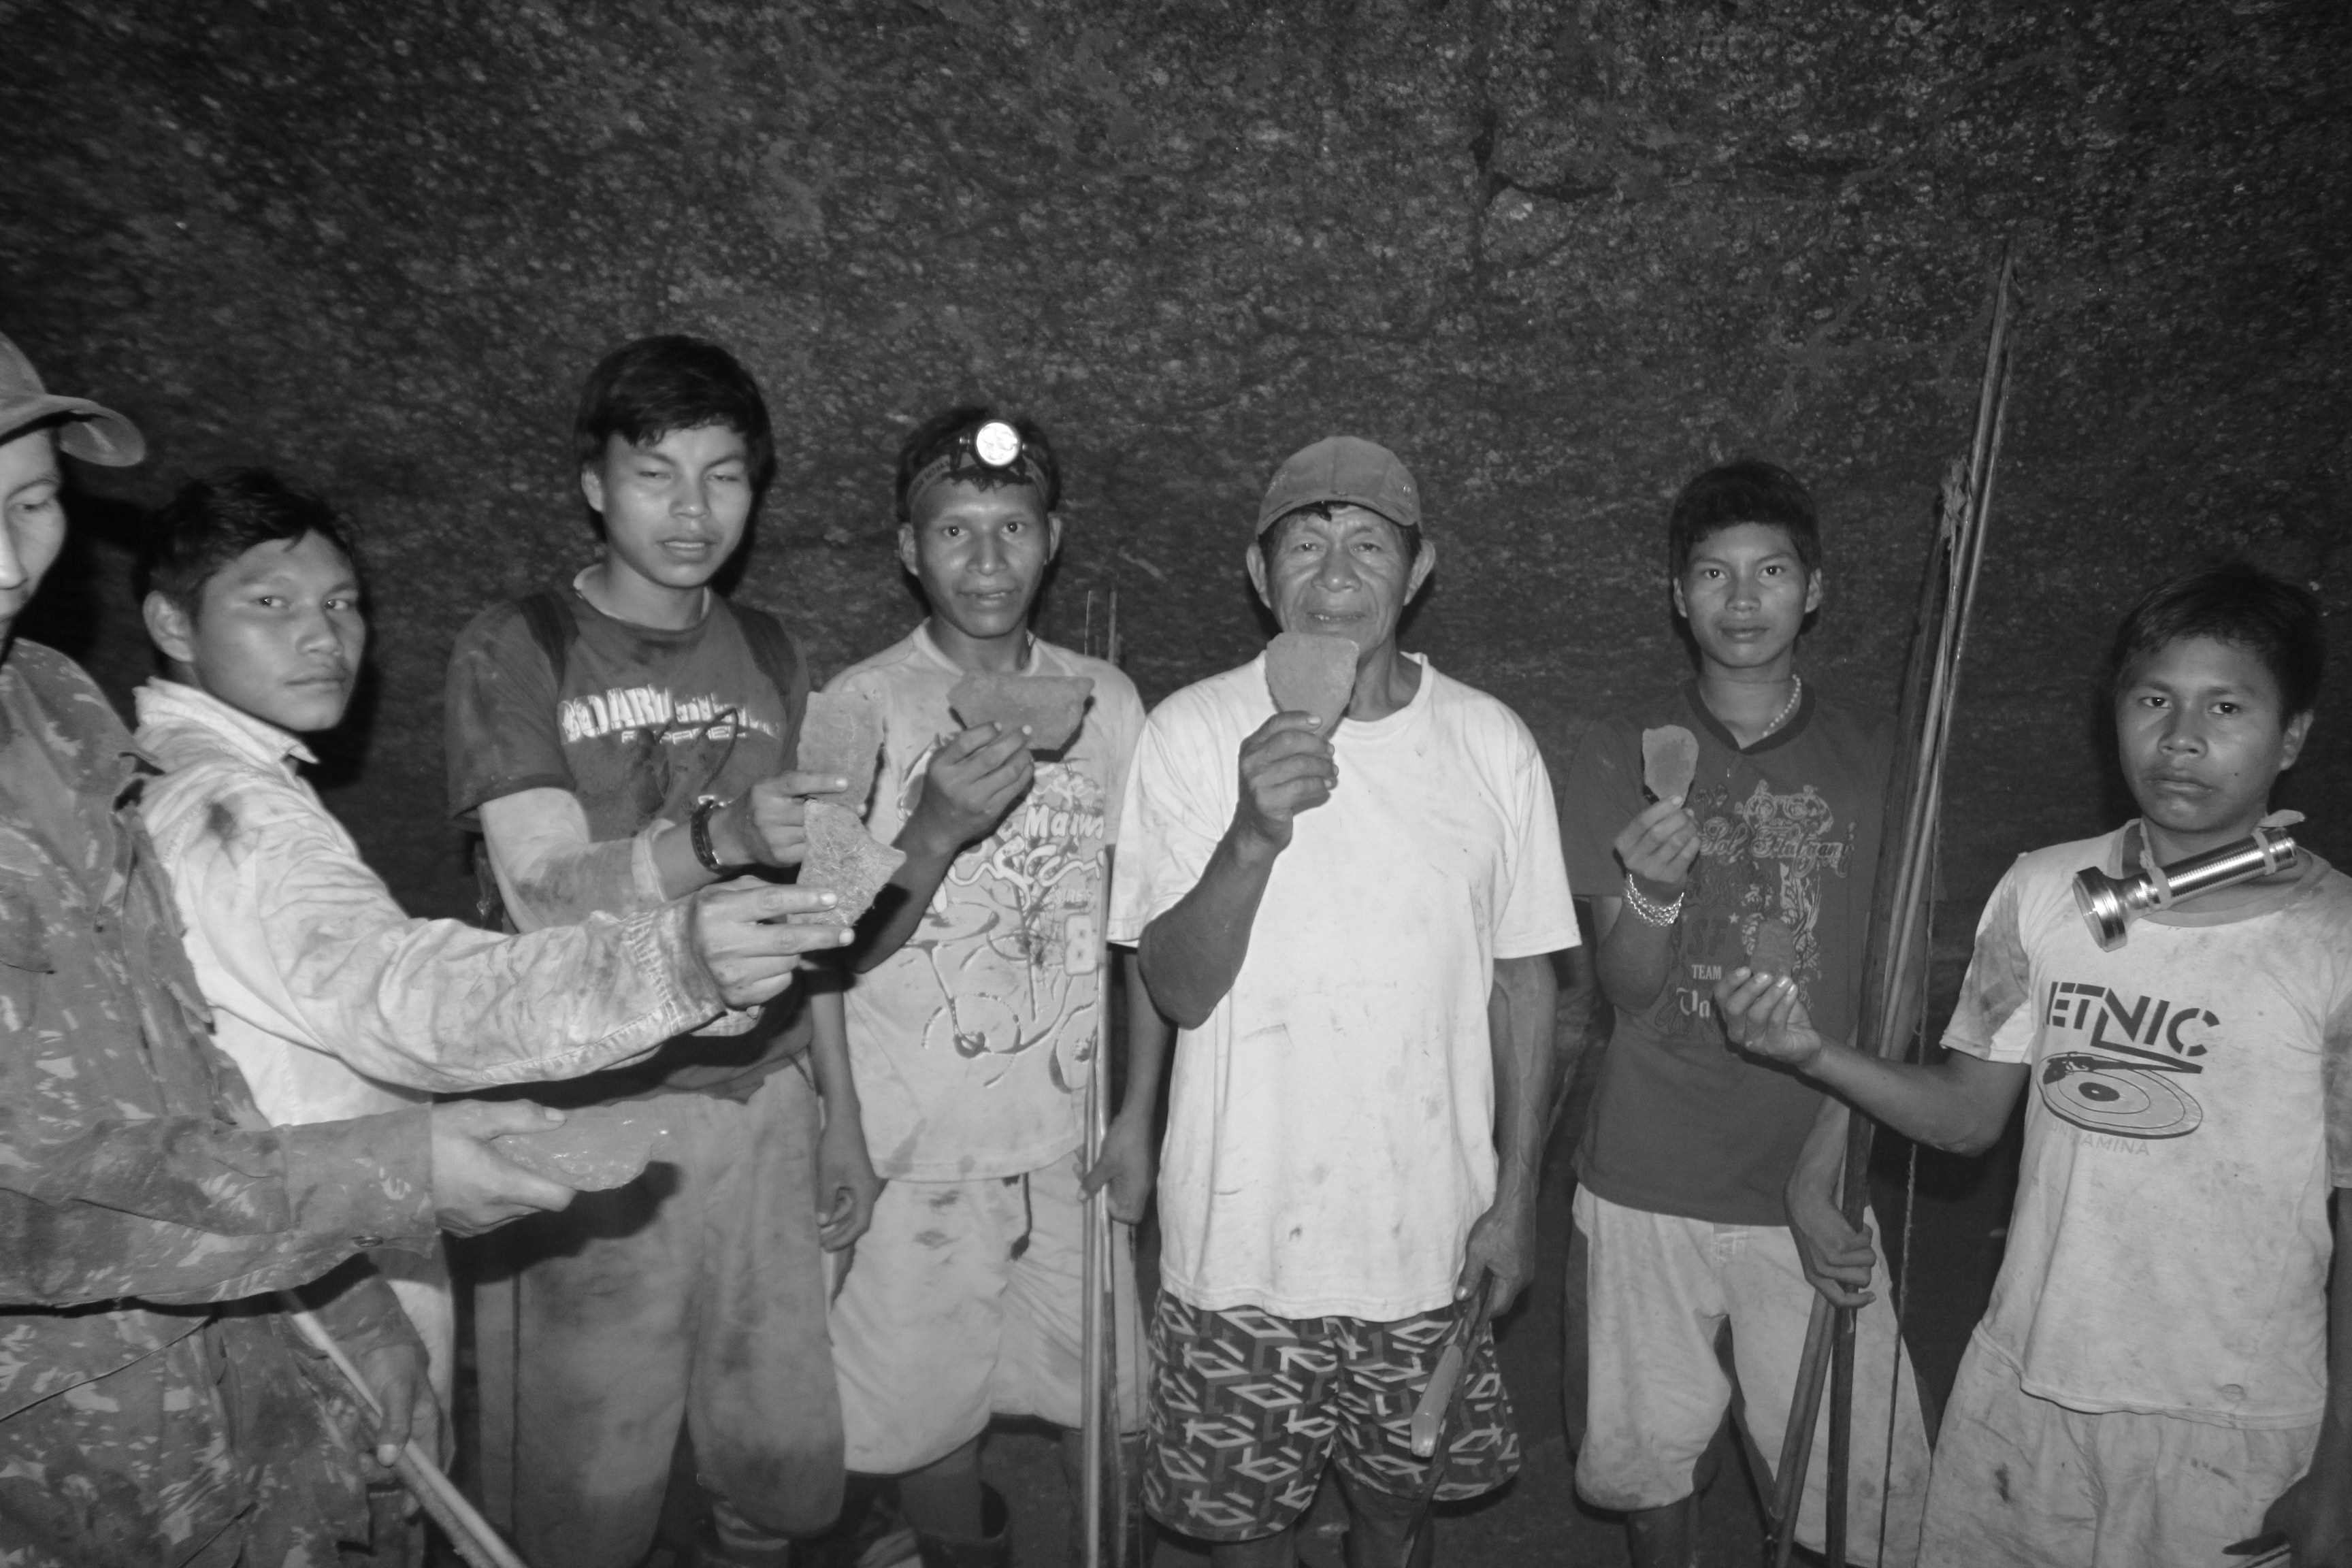
\includegraphics[width=\textwidth]{./img/017}
%\caption{Viajantes exibem as lascas de cerâmica (foto: Danilo P. Ramos, 2012)}
%\end{figure}

Assustado, olhando fixamente para ao chão, Ari chamou Ponciano:
\textit{Guerrilhero s'i̖b}, ``pegada de guerrilheiro'' exclamava. Sem dúvida era
o vestígio de um pé humano descalço, cuja marca ainda estava fresca. Não
estávamos sozinhos naquele local. Ainda hoje é possível ouvir boatos
sobre a presença dos guerrilheiros. Ex"-membros das antigas Forças
Armadas Revolucionárias Colombianas (\textsc{farc}), eles buscam refúgio nos
morros para esconder"-se do exército brasileiro. Antes de nossa partida
de \textit{Ta̗t"-Dëh}, os principais temores dos viajantes eram o encontro com
onças e com os guerrilheiros, por haver muitas notícias de sequestros de
rapazes indígenas pelas milícias. Temerosos da violência que esses
brancos poderiam praticar contra nós, encurtamos nossa visita e descemos
apressadamente o morro para retomarmos nosso percurso rumo a \textit{B'ö̖'"-Paç}.

Atordoados com o sinal de presença do guerrilheiro, deixamos
\textit{Ni̗k"-Hu̗͂-Paç}. Paramos no \textit{Kaya̖'"-dëh}, pequeno igarapé próximo, para
pescar e saciar a fome. No caminho, passamos por uma clareira na mata.
Ponciano parou e revelou que esse havia sido o local de morada do
ancestral \textit{Yo̗k}, Lontra, depois de sua partida de \textit{D'ö̖p"-Dëh}. Viera
com a família, sua esposa e filhos. Construíra o telhado de sua casa com
penas de \textit{yë̖ç}, ``jacuaçu''.\footnote{\textit{yëç}, ``jacuaçu'': certo tipo de
  ave da família dos cracídeos, \emph{Penelope jacquacu.}Cf. Ramirez
  (2006).} ``Nesse tempo não havia caranã e se fazia muito essas \textit{Yë̖ç
Pãt Mo̖y}, Casas"-de"-Pena"-de"-Jacuaçu\,'', explicou. O mesmo local era
também uma Morada Antiga onde os familiares de Ponciano vieram viver.
Ainda no caminho passamos por um lamaçal. Nossos pés atolavam a cada
passo e seguíamos com dificuldade. José contou que, ali, a ancestral
\textit{Tud"-Asa̗w} jogava água e lama nos rapazes para seduzi"-los.

Andamos por cerca de uma hora até encontrarmos a base da Serra do
Tucunaré, \textit{B'ö̖'"-Paç}. Diferente dos dois outros morros, esse
apresentava uma vegetação mais rasteira, composta principalmente por
arbustos. O solo, como nos outros morros, era de \textit{paç s'a̗h}, ``terra de
serra'', considerada extremamente fértil: \textit{paç s'a̗h tuhu̗p}, exclamava
Ponciano, ``a terra da serra é ótima''. Quando era criança, seu pai
tinha uma roça em \textit{B'ö̖'"-Paç}. Tombou"-a logo que se mudou de \textit{Pi̖j"-Dëh}. A
terra de \textit{B'ö̖'"-Paç} era tão boa que tudo o que se plantava crescia:
cana, abacaxi, maniva, banana. Ponciano mostrou o lugar onde seu pai
costumava fazer a barraca para eles abrigarem"-se enquanto realizavam
seus afazeres agrícolas. Aparentava estar muito feliz em guiar"-nos por
aquelas searas.

Ponciano levou"-nos para visitar uma das grutas desse morro que disse ser
outra Morada"-de"-Semente de Tabaco onde havia um \textit{ho̗n"-hö̖d}. O filete
de água a escorrer pelo chão, a luminosidade e o piso de areia clara
pareciam dar contornos a esse cenário ideal para a prática xamânica.
Ponciano, Ari e eu abaixamo"-nos e bebemos um pouco da água: \textit{käh, käh
hisa̗p, tuhu̗p}, ``doce, muito doce, pura'', exclamaram. Como o líquido do
maracujá em \textsc{b5}\index{af@\textsc{b}5\quad \textit{Ti̖wi̖t hamap bi'i̖d ta'}\break Benzimento dos caminhos}, essa água possui princípios que curam e
purificam o corpo, sendo considerada uma \textit{yõ̖h"-dëh}, uma ``água"-pura''.
Ingerindo grandes quantidades dessa água, o pai de Ponciano vomitava
para limpar o corpo do \textit{nag}, ``óleo'', que há na carne de caça e no
peixe moqueado, e que, com o tempo, suja o corpo e a orelha. Quando era
mais jovem, Ponciano chegou a fazer esses retiros para sonhar.

No dia seguinte, visitamos ainda outra Morada"-de"-Semente de Tabaco
em \textit{Hõpo̖y"-Paç}, Serra do Surubim. A gruta assemelhava"-se às outras
três visitadas. Fora também um \textit{ho̗n"-hö̖d} dos antigos, onde bebiam água,
vomitavam, dormiam e sonhavam com os ancestrais. Mais uma vez, Semente
de Tabaco havia deixado os restos de seus utensílios de cozinha
esparramados pelo chão. As lascas de cerâmica dispersas na areia
chamaram a atenção dos viajantes, que começaram a observá"-las. Saindo
dessa gruta, Ponciano contou de um ancestral, \textit{B'ö̗b tẽh}, Tururi,
que, como Semente de Tabaco, habitara esse morro. Fez sua casa, mas não
conseguia encontrar comida. Ele, então, esfregou sua colher no chão. O
barulho gerado pelo atrito fez os peixes aparecerem no rio e, assim, ele
pode pescar e saciar sua fome.

Nesse momento já nos aproximávamos de outra caverna. A formação rochosa
era menor que as outras e mais clara. Paramos para descansar um pouco e
todos quiseram que eu tirasse uma foto do grupo. Quando saíamos,
Ponciano matou uma jararaca com seu terçado. Aquilo que para nós
aparecia como uma cobra era, na verdade um \textit{b'atɨ̖b'} rastejando vestido
com sua roupa de jararaca: \textit{Nu̗p paç, b'atɨ̖b' nɨ̖h mo̖y}, ``essa
Casa"-de"-Pedra é morada de \textit{B'atɨ̖b'}''. Deixamos a \textit{Hõpo̖y"-Paç} e
retornamos às margens do \textit{Ya̖k"-Dëh}, Arara"-Igarapé, onde pescamos e
repousamos para visitar a Serra da Paca, \textit{Hu͂ya̗w"-Paç}, no dia
seguinte.

Nesses \textit{ho̗n"-hö̖d}, como nos aprendizados oníricos dos comedores de coca,
os sonhadores caminhavam até as Casas"-de"-Pedra, ingeriam água, dormiam e
viajavam para encontrar"-se com seus antepassados e ouvir encantamentos.
Esse processo de aprendizado podia durar semanas e ser realizado
individual ou coletivamente. Comiam pouco, alimentando"-se apenas de
beiju e farinha. Essa forma específica de interação realizava"-se a
partir de um afastamento do convívio da aldeia e dos afazeres diários
para uma aproximação aos antigos. Ocorria antes dos Dabucuri e das
grandes festas de caxiri que reuniam pessoas de diferentes aldeias.
Depois desses dias de retiro, os xamãs retornavam à comunidade e
participavam das festividades. Purificados e tendo aprimorado suas
habilidades, adquiriam mais força para cercar suas famílias, que durante
as celebrações estavam mais suscetíveis às brigas e aos feitiços.

De modo surpreendente, a Casa"-do"-Trovão é tida como uma \textit{Paç"-Mo̖y}, uma
Casa"-de"-Pedra celeste. Lá são as Onças que realizam as práticas
xamânicas. Observando o desenho feito por Samuel, é possível ver uma
casa que é, ela mesma, uma serra constituída por três morros. O primeiro
deles, à esquerda, trata"-se da morada dos homens cuja porta é aberta
para o sol nascente. Essa casa é denominada \textit{Dëh"-Sa̗ka̗n"-Du̗y"-Mo̖y},
Casa"-do"-Sol"-Nascente. Como as casas dos brancos, essa casa possui
janelas. O piso de areia faz com que a cor amarela predomine, irradiando
sua luminosidade para as portas e janelas. No meio, há uma casa onde
todos os dias as Gentes"-Onça oferecem a coca a seu dono, o Trovão. É lá
também que estão guardadas as flautas sagradas, os Jurupari do Trovão e
das Gentes"-Onça. Essa casa é denominada \textit{Dëh"-K'et"-Yoh"-Mo̖y},
Casa"-da"-Cabeceira. À direita, está a casa das mulheres com uma porta
e janela menores voltadas para o pôr do sol. É considerada a cozinha e,
por isso, recebe o nome de \textit{Po̗ho̗y"-Mo̖y}, Casa"-da"-Fermentação, algo
que alude ao preparo do caxiri feito pelas Mulheres"-Onça e
Mulheres"-Trovão.

%\begin{figure}
%\centering
%\includegraphics[width=\textwidth]{./img/018}
%\caption{Casa"-do"-Trovão (desenho M'e̖h Sɨh/Samuel Brasil Monteiro, 2012)}
%\end{figure}

Assim, a arquitetura celeste da Casa"-do"-Trovão torna"-se especialmente
interessante para refletir sobre as Casas"-de"-Pedra dos ancestrais hup. O
chão de areia das Moradas de Semente de Tabaco é como aquele da
Casa"-do"-Trovão. É principalmente o ato de entrar na caverna que
transforma as grutas em moradas. Em \textsc{m13}\index{22@\textsc{m}13\quad A dádiva da coca e do tabaco}, a Serra da Cutivaia
passa a ser uma morada de Semente de Tabaco após sua entrada. Do mesmo
modo, fugindo da Anta, a Cutivaia esconde"-se na caverna dessa serra,
transforma"-se numa onça que passa a habitar e a dominar o morro
(\textsc{m12}). A entrada dos xamãs hup nas cavernas para beber água,
vomitar, dormir e sonhar transforma os \textit{ho̗n"-hö̖d} em moradas que abrigam
os senhores hup nesses períodos de afastamento de suas aldeias. Se é na
\textit{Dëh"-K'et"-Yoh"-Mo̖y} que o Trovão e as Onças comem coca e guardam suas
flautas Jurupari, as cavernas nos morros são igualmente
Casas"-da"-Cabeceira para os Hupd'äh, onde práticas rituais levam ao
aprendizado onírico com os ancestrais e à maior capacidade dos xamãs em
cercar suas comunidades durante as cerimônias em que as flautas Jurupari
são tocadas. No xamanismo desana, o poder de entrar é descrito por
Reichel"-Dolmatoff da seguinte maneira,\index{21@\textsc{m}12\quad A Anta e a Cutivaia}

\begin{quote}
O poder de \textit{penetrar} possui várias interpretações. Por um lado,
possui um sentido visual, de ver o que está oculto para os demais. Por
outro lado, possui uma interpretação sexual, pois o pajé {[}\ldots{}{]}
representa um conceito fálico de procriação. Outro aspecto do poder de
\textit{penetrar} é a capacidade do êxtase e do voo mágico que permite ao
pajé sair da biosfera e \textit{penetrar} outro plano existencial. Um pajé é,
no fundo, o especialista em realizar essa ruptura de nível, tanto num
sentido extático espacial, quanto no sentido de passar de uma unidade
conceitual de tempo à outra, já que o êxtase equivale à morte e é,
assim, um processo de aceleração do tempo.\footnote{1986, p.\,156.}
\end{quote}

Dessa forma, entrar na caverna é penetrar a Morada"-de"-Semente de Tabaco.
É também um movimento que configura a caverna como uma maloca, própria
para as práticas rituais dos antigos nos \textit{ho̗n"-hö̖d}. A ingestão das águas
e o vômito possibilitam o deslocamento onírico, o \textit{voo mágico} através
do qual os praticantes veem os ancestrais, conversam e aprendem como se
estivessem sentados em rodas de coca. Entrando nos morros, os viajantes
atravessam \textit{unidades temporais} e fortalecem"-se, crescem ouvindo as
palavras dos ancestrais. As cavernas existem antes da entrada dos seres
e dos ancestrais hup, e é esse ato de entrada que as torna
Casas"-de"-Pedra e lugares sagrados próprios para a habitação e para a
prática ritual.

Antes de entrar na caverna, Semente de Tabaco deixa o cigarro e a coca
como alimentos para seus sucessores. Esses \textit{alimentos da origem}
permitem ver e conversar sobre as histórias e encantamentos, algo que
constitui uma gênese das rodas de coca. Todas as noites, com o término
do encontro noturno, os senhores hup juntam os utensílios culinários,
panelas, cuia, pilão, num canto da cozinha coletiva e deixam"-nos assim
para a roda do dia seguinte. De forma semelhante, os restos dos
utensílios culinários de Semente de Tabaco foram deixados ao lado dos
\textit{ho̗n"-hö̖d}, algo que possivelmente remete à prática emética do ancestral.
Dessa forma, as lascas de cerâmica no chão arenoso dessas nascentes de
igarapés parecem apontar para outra dádiva de Semente de Tabaco, a dos
\textit{ho̗n"-hö̖d}. Também esse ancestral bebia, comia e dormia nesses espaços.
Tocando as lascas de cerâmica e observando"-as atentamente, os viajantes
ouviam a história contada por Ponciano. Os artefatos, formas produzidas
ao longo do processo de habitação de Semente de Tabaco, iam sendo
remodelados pela Casa"-de"-Pedra. Nas mãos dos rapazes, as lascas
tornavam"-se espécies de pegadas, rastros para uma observação atenta
proporcionada pelas palavras do mentor.

Analisando o processo de ingestão de yagé e caxiri dos Barasana, C.
Hugh"-Jones ressalta que:

\begin{quote}
O vômito, induzido pela ingestão de yagé e caxiri durante o canto,
também ocorre no lugar masculino no fundo da maloca. Beber yagé e
vomitar, ouvir discursos e respondê"-los, inspirar e expirar são todos
processos de dois sentidos envolvendo entrada e saída pela boca (ou
orelhas). Esses processos são também associados às idas e vindas através
da porta dos homens e a processos rituais de regeneração patrilinear.\footnote{C. Hugh"-Jones, 1976, p.\,199.}
\end{quote}

\index{ab@\textsc{b}1\quad \textit{Pũ'ũ̖k bi'i̖d}\break Benzimento da coca}
Nos \textit{ho̗n"-hö̖d}, a água entra pela boca e por ela saem as impurezas
causadas pelo barulho do Trovão e pelos alimentos moqueados. Como no
benzimento da coca (\textsc{b1}), que faz surgirem orifícios nos pés
para a saída da gordura e pasta, a água doce transforma"-se no estômago,
absorve a sujeira e purifica o ouvido para que, na Casa"-da"-Audição, a
semente"-do"-ouvido esteja limpa e possa crescer com as palavras ouvidas
dos ancestrais em sonho. Há, nesse sentido, um processo ritual de
regeneração patrilinear proporcionado pelo caráter irreversível da
digestão. A ingestão das águas que absorvem a sujeira e a doença é uma
\textit{super"-digestão} capaz de fazer as impurezas não digeridas dos
alimentos saírem pelo orifício bucal.

Segundo a descrição de Reid, o Trovão coabita a zona superior do cosmos
com \textit{K'e̖g Te͂h}. É tido como o responsável pelo aparecimento das doenças
e das formas de curá"-las. De forma semelhante, o antropólogo menciona
que para prevenir a entrada de doenças causadas pelos trovões, os
Hupd'äh tapam os ouvidos. No esquema cosmográfico proposto por Reid,
abaixo desse nível superior haveria um cinturão rochoso, uma zona
central, habitada por Onças.\footnote{Conforme o mito \textsc{a}, transcrito por
  Reid, as Onças teriam sido lançadas a essa região celeste pelo sopro
  dos \textit{Biyoo Kagn Teindʉ}, Diruá, em vingança pela morte de seus pais,
  devorados pelas feras. Para a realização de sua vingança, os irmãos
  órfãos receberam do Trovão bastões para causarem trovões. Foi o Trovão
  quem deu aos Diruá a pintura facial e os alucinógenos como poderes
  (Reid, 1979, p.\,232- 233).} As Onças são capazes de gerar trovões e,
assim, causar doenças. São controladas pelo Trovão, visto como um dono
dos xamãs. Como enfatizavam meus companheiros, quando o Trovão e as
Onças deixam de reunir"-se na Casa"-da"-Cabeceira para comer coca,
formam"-se as nuvens de chuva (água celeste).\footnote{Lévi"-Strauss
  analisa a oposição entre água terrestre e água celeste para a análise
  dos mitos Warrau (2004b, p.\,204).} A tempestade atrapalha as rodas de
coca hup, suja o ouvido e causa doenças. Por outro lado, bebendo a água
das serras (água terrestre), os xamãs limpam seus ouvidos da sujeira.
Dessa forma, mandar a tartaruga para a Casa"-da"-Cabeceira afasta as
nuvens para os morros, nascentes dos rios, permite que os senhores hup
se reúnam nas rodas e talvez faça também com que as Onças voltem a
oferecer coca a seu dono.

Vimos no capítulo anterior que o nome de uma das casas situadas às
margens do Lago de Leite é justamente \textit{Pe̗͂y"-Mo̖y}, Casa"-do"-Trovão. Como na
arquitetura celeste, fazem parte da paisagem da origem uma
Casa"-do"-Trovão, uma Casa"-do"-Sol"-Nascente e uma Casa"-da"-Cabeceira. Se,
como Samuel contou, há um Lago de Leite na maloca quando as flautas
Jurupari são tocadas, há também uma porta para o nascer do sol e outra
para o pôr do sol. As colunas que sustentam o telhado são como os morros
que alicerçam o céu quando a maloca se torna um espaço masculino
interditado às mulheres. Essa interdição faz pensar na divisão sexual
das moradas na Casa"-do"-Trovão. Ao mesmo tempo, a maloca transforma"-se em
Casa"-da"-Fermentação com a entrada das panelas de caxiri das mulheres, as
danças e as conversas. Desse modo, é possível ver os \textit{ho̗n"-hö̖d} como
locais de afastamento de homens com relação às mulheres, isolando"-se
numa Casa"-da"-Cabeceira, como o Trovão e seus cunhados.

A água com que nos banhamos no lago do alto da Serra Grande era uma água
de chuva represada pelo orifício da superfície rochosa. Essa água
celeste no \textit{topo do mundo} purificava nossos \textit{hã̗wäg} e endurecia
nossas peles tornando"-as resistentes como paris ou cascas de turi. Após
a segunda viagem à Serra Grande, é possível aos andarilhos beber a água
do lago que age como um \textit{caarpi}, gerando sonhos e fazendo com que a
pessoa encontre ancestrais e aprenda mitos e encantamentos. Doce como a
coca (\textsc{b1}), a água que escorria pelos \textit{ho̗n"-hö̖d} era capaz de
causar vômitos para limpar e purificar. De forma parecida, essa água das
nascentes faz sonhar, como o \textit{caarpi} e a água do lago da Serra Grande.
Assim, os fios de água dos \textit{lugares de vomitar} são fontes de
água"-pura que preparam o corpo para a mobilidade e encontro oníricos.
\index{ab@\textsc{b}1\quad \textit{Pũ'ũ̖k bi'i̖d}\break Benzimento da coca}

Nesse sentido, talvez a força e o perigo da água da Serra Grande esteja
no fato de ser essa uma água celeste e, assim, uma água do Trovão. Beber
a água nos \textit{ho̗n"-hö̖d} é consumir a água da nascente, a água de uma
Casa"-da"-Cabeceira, algo que remete ao poder do Trovão de fazer a chuva e
as tempestades a partir de sua morada celeste. Nuvens e cabeceiras são,
portanto, nascentes de águas celeste e terrestre. Bebendo a água das
cabeceiras, os xamãs viajam oniricamente e encontram"-se com seus
ancestrais. Bebendo a água do Trovão (Serra Grande) represada como um
Lago de Leite, os senhores hup aproximam"-se da potência desse ser, algo
perigoso, desafiador e importante para o desenvolvimento xamânico.
Rumando para a cabeceira, a tartaruga dirige"-se para a nascente
terrestre das águas, age sobre a nascente celeste e, de certo modo,
reverte o impacto da ação maléfica do Trovão.

As Casas"-de"-Pedra são pontos fixos para os movimentos de seus ocupantes
e visitantes, ninhos e abrigos para onde os seres retornam regularmente.
Essas Casas"-de"-Pedra são organismos vivos cujas histórias são
desdobramentos de suas relações com humanos e seres diversos. Aceitando
caminhar aos morros, os viajantes iniciavam uma jornada ao desconhecido
desses centros nodais, plenos de forças primordiais e aterradoras.
Penetrando as cavernas, os andarilhos recriavam"-nas como Casas"-de"-Pedra
e recriavam"-se a si mesmos como filhos de Semente de Tabaco. Os rastros
do ritual xamânico praticado desde o tempo de Semente de Tabaco e as
cavernas tornam"-se vistas; o deslocamento entre uma vista e outra gera
transições que, como ocorre com a passagem do xamã de casa em casa
(\textsc{b5}), descrevem percursos de movimento, de percepção e de ação
ao longo de caminhos vividos. Percorrendo tais caminhos e bebendo a água
das nascentes, os rapazes vão seguindo os passos de seus predecessores e
posicionando"-se na matriz dos movimentos que constituem a região das
cabeceiras e estende"-se até a Casa"-do"-Trovão.
\index{af@\textsc{b}5\quad \textit{Ti̖wi̖t hamap bi'i̖d ta'}\break Benzimento dos caminhos}

\section{Na pele da onça}\label{na-pele-da-onuxe7a}

No dia 12 de março de 2012, quando deixamos a morada de Semente de
Tabaco de \textit{Ni̗k"-Hũ̗-Paç}, continuamos a explorar um pouco mais o morro,
dirigindo"-nos à sua área central. Valter, que andava à frente, ouviu um
barulho, como que um rugido de onça. Todos nós ficamos atentos. O rapaz,
corajosamente, seguiu adiante para ver o que era. Voltou esbaforido
dizendo que havia uma onça"-preta, uma \textit{ya'a̗m s'a̗}, deitada bem
naquela direção. Olhamos amedrontados e vimos o vulto negro que nos
observava à distância. Sem pensar duas vezes, começamos a correr para
nos afastarmos o mais depressa possível. Ponciano conservava sua mão na
flecha envenenada, caso o animal avançasse. Percebendo que ela não nos
perseguia, recuperamos o fôlego para chegarmos ao pé do morro com mais
calma.

Dias mais tarde, na festa de caxiri em comemoração a nosso retorno,
sentamos para conversar com o pajé Armando. Entre uma cuia e outra,
antes que contássemos de nosso terrível encontro com a onça, o xamã
revelou que havia nos acompanhado durante toda jornada. Ao longo
daqueles dias em que caminhávamos, ele consumiu paricá e viajou com seu
\textit{hã̗wäg} para as serras. Movia"-se dentro de sua roupa de \textit{ya'a̗m s'a̗},
``onça"-preta'', e nos observava de longe. Rindo, contou que o tínhamos
visto no alto de \textit{Ni̗k"-Hũ̗-Paç} e que corremos de medo. Olhando em meus
olhos e afagando minha barba, Armando disse que meu bigode era de onça.
Meu cheiro, de branco, podia ser sentido à distância pelas onças e pela
\textit{Dö̗h Ã̗y}, o que tornara nossa viagem muito perigosa. Por isso, ele teve
que nos acompanhar, seguir conosco \textit{hã̗wägat}, viajando como
pessoa"-sopro, com seu \textit{se͂he̖͂k hãwäg}, ``sopro de paricá''.

\index{af@\textsc{b}5\quad \textit{Ti̖wi̖t hamap bi'i̖d ta'}\break Benzimento dos caminhos}
Em \textsc{b5}, é para o corpo da ``onça pequena'' \textit{dɨ̗d} que se dirige o
benzedor. Ele penetra também o corpo do esquilo marrom. Assume as formas
corporais de um peixe"-cobra, o muçum (água), de uma ave pequena, o curió
(ar), e dos calangos (terra). Os últimos vivem em terrenos secos, tendo
permanente contato com o chão. A transmutação e penetração corporais são
procedimentos fundamentais para a proteção, para o deslocamento e para o
contato seguro do xamã com os seres malfazejos. Observando"-nos de longe,
Armando protegia"-nos. Fez"-se visível para mostrar que não estávamos
sozinhos e para assustar"-nos. Consumindo o paricá em sua casa, ele
vestiu sua ``roupa de onça'', \textit{ya'a̗m yu̖d}, e seguiu viajando pelos
caminhos para acompanhar"-nos. Sua jornada dava"-se a um só tempo
\textit{hã̗wägat}, ``indo como pessoa sopro'', e \textit{sa̗pa̗t}, ``indo como
pessoa"-onça corporificada''. Sobre o xamanismo Desana,
Reicheil"-Dolmatoff afirma que:

\begin{quote}
A transformação em jaguar poder ter dois objetivos: ou o pajé se
converte em jaguar para proteger uma maloca ou a um caçador solitário
contra os perigos, caso no qual o jaguar se mantém invisível para os
seres humanos e é percebido apenas pelos seres sobrenaturais; ou se
converte visivelmente em jaguar {[}\ldots{}{]} e ataca um inimigo.\footnote{1986, p.\,163.}
\end{quote}

De forma semelhante, a transformação do pajé hup em jaguar tem o
objetivo de proteger o grupo de viajantes dos perigos. Conforme me
explicou Samuel, as \textit{yu̖d}, ``roupas cósmicas'', são poderes fundamentais
para a agência xamânica de benzedores e pajés. Permitem seu deslocamento
entre os diversos planos"-casa e sua segurança durante a interação com
outros seres. Gentes"-Árvore, \textit{B'atɨ̖b'}, Gentes"-Cobra, \textit{Dö̗h Ã̗y}, todos
possuem roupas e são capazes de vesti"-las para assumirem outras
perspectivas, circular pelo cosmos e fazer mal aos Hupd'äh. Esse foi o
caso do \textit{b'atɨ̖b'} que Ponciano matou com seu terçado quando deixávamos
\textit{Hõpo̖y"-Paç}. A capacidade de diferenciar a serpente do ser malfazejo,
vestido, parece ser uma habilidade comum a muitos xamãs hup que
evidencia um modo de percepção atento à presença e aos poderes de
transmutação e penetração corporais dos seres. Assim, saber vestir"-se
com a roupa de onça e penetrar os corpos do esquilo marrom, do muçum e
do lagarto é também saber identificar a habilidade de metamorfose dos
outros seres a partir de suas roupas cósmicas. Analisando as roupas
cósmicas wauja, Barcelos Neto salienta que:

\begin{quote}
A \textit{roupa} é um dispositivo de atributos instrumentais e anatômicos ---
asas, no caso dos seres alados, garras e/\,ou presas, no caso dos
predadores, etc. --- que enseja capacidades físico --- locomotoras
específicas: voar, nadar, saltar, correr velozmente etc. Os humanos são
naturalmente os sem"-\textit{roupa}, com exceção dos feiticeiros, que podem
fazer uso de \textit{roupas} especiais chamadas \textit{iyeyá} para entrar nas
casas de outras pessoas ou viajar a grandes distâncias em curtíssimo
tempo. Uma \textit{roupa} sempre envolve consequências práticas imediatas,
pois ela é uma forma funcional: dentes e garras afiadas, nadadeiras,
bicos alongados etc., coisas que servem para realizar tarefas
específicas, as quais os humanos fazem com o auxílio de uma série de
artefatos, muitos deles originalmente criados pelos \textit{yerupoho}
{[}\ldots{}{]} e posteriormente transferidos para o mundo dos humanos
via doenças, xamanismo e ritual.\footnote{2008, p.\,69.}
\end{quote}

No caso da roupa de onça, o grau de poder varia de acordo com o tamanho
e a capacidade destrutiva da fera. Os pajés possuem roupas de onças
grandes, mas apenas os mais poderosos vestem as roupas da temida
onça"-preta. Enquanto a maior parte das onças se inibe diante de um grupo
de caçadores, essa parece ser a única variedade que não demonstra medo e
ataca ainda que esteja em desvantagem. A roupa de onça"-preta revela o
poder de Armando e sua capacidade de proteger"-nos durante a viagem. Como
no xamanismo wauja, além dos dentes e garras afiadas, ao vestir"-se com a
roupa de onça, o xamã leva consigo o arco e flecha, a lança e a faca
felinas, armas que fazem dele um poderoso caçador"-guerreiro. Segundo
Reid,\footnote{1979, p.\,264.} ``No pensamento Hupdʉ, os jaguares também são
associados muito intimamente aos xamãs, que, embora sejam reconhecidos
como humanos, ocupam a mais ambígua e marginal das posições na sociedade
humana''.

%\begin{figure}
%\centering
%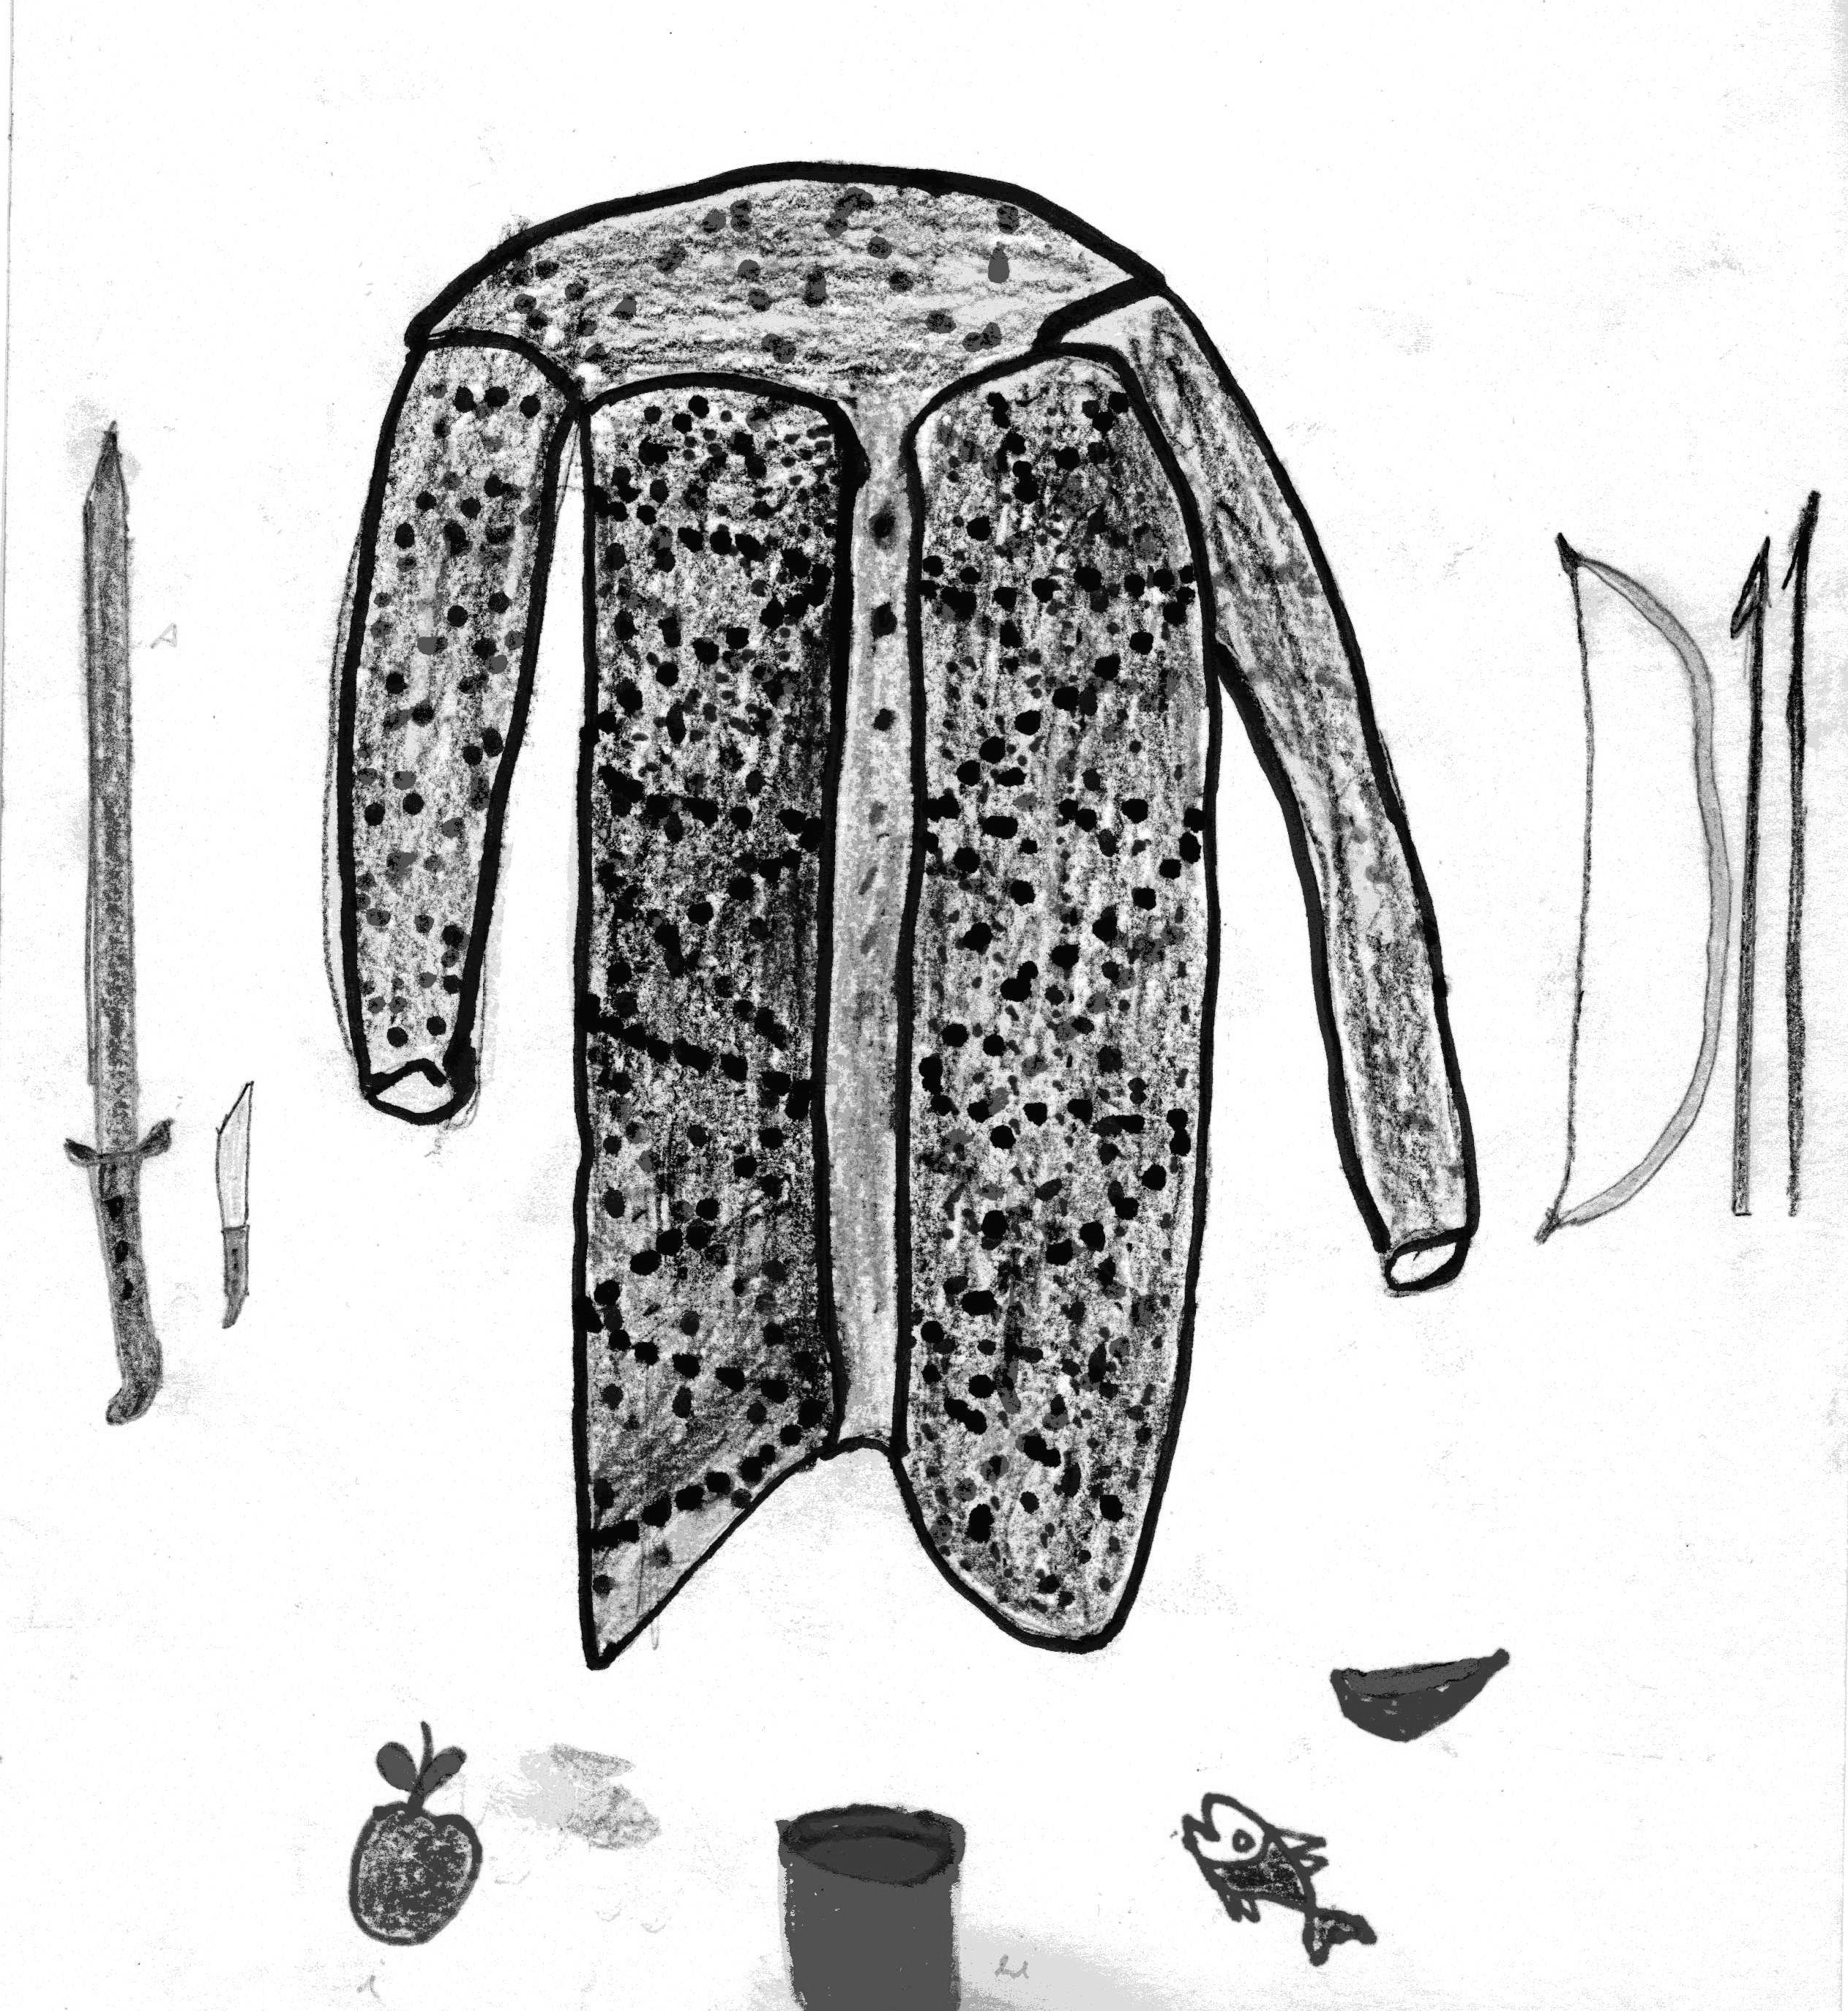
\includegraphics[width=\textwidth]{./img/019}
%\caption{Roupa de onça, armas e alimentos (Desenho: /M'e̖h Sɨh/ Samuel Brasil Monteiro)}
%\end{figure}

\index{af@\textsc{b}5\quad \textit{Ti̖wi̖t hamap bi'i̖d ta'}\break Benzimento dos caminhos}
Em \textsc{b5}, penetrando a onça pequena, Ponciano mostra"-se igualmente
como um poderoso \textit{kä̖d hup ĩh}, já que poucos \textit{xamãs"-do"-banco} são
capazes de vestir roupas de onça. A onça \textit{dɨ̗d}, jaguatirica, pode ser
vista como sendo o menor felino a viver na planície amazônica.\footnote{Diferente
  da classificação zoológica que diferencia a jaguatirica (\emph{felis
  pardalis}) do restante das onças (\emph{panthera onca}), os Hupd'äh
  incluem"-na na mesma categoria denominando"-as \textit{ya'a̗m te͂h} (Emmons,
  1990).} Envolto em seu corpo, o benzedor transita entre os diversos
\emph{planos"-casa} em segurança, mas sua capacidade de predação é
notavelmente inferior àquela dos pajés. Vestidos com suas roupas de
onça, os xamãs viajam pelos caminhos numa rapidez muito superior à dos
\textit{passos de hup}. Partindo da reflexão de Viveiros de Castro (2002), os
corpos das onças servem como modelos para que os humanos se vistam e
para que os animais se dispam de suas vestes animais e revelem sua
essência humana.\footnote{Viveiros de Castro, 2002, p.\,389.}

A onça"-pintada (\emph{Panthera onca}) é considerada o maior felino da
América do Sul, mas as que habitam as florestas tendem a ser menores que
aquelas que habitam áreas abertas. Seu peso varia entre 35 e 130 kg, e
seu tamanho entre 1,7 e 2,4 metros. O corpo musculoso e ágil permite ao
animal o deslocamento rápido e a precisão no ataque às presas. A cor de
sua pelagem varia do amarelo"-claro ao castanho"-ocreáceo, sendo
caracterizada por manchas (rosetas) pretas espalhadas por todo o corpo.
As onças que possuem pelagem preta e manchas são denominadas
onças"-pretas. As características específicas da garganta do felino, que
possui uma ossificação incompleta do osso hioide, permitem que ele emita
esturros, sons fortes e graves, fundamentais para a comunicação com
outros indivíduos, principalmente no período reprodutivo. Sendo as onças
animais solitários e territoriais, são principalmente os esturros e o
odor das fêmeas que permitem aos machos localizá"-las para a interação e
reprodução. A urina, as fezes e os arranhões em árvores são as marcas
que delimitam a área de vida do animal. As onças que vivem em áreas de
floresta atuam principalmente durante o dia. Apesar da grande capacidade
de predação do felino, que chega a alimentar"-se de 85 espécies na região
amazônica, as onças buscam principalmente grandes mamíferos --- como
queixadas, tamanduás, capivaras, antas --- e répteis --- como os jacarés e
as tartarugas.

Para os viajantes, os sinais da presença de onça são percebidos pelo
forte odor de sua urina, pelo som grave de seus esturros, pelas pegadas
deixadas no chão, pelo estrondo dos banhos noturnos da fera e pelos
restos de pelo das presas devoradas. Aquele que caminha pode ser
surpreendido pelo ataque de um felino que surge repentinamente do meio
da mata. Uma das formas de ataque mais temidas é o pulo do predador que
fica à espreita no alto das árvores e, conforme o caminhante passa,
lança"-se contra a presa ferindo"-a em sua nuca e costas. No que diz
respeito à comensurabilidade, há a interdição de consumo das onças
grandes. Entretanto, as onças pequenas, que se alimentam de herbívoros,
podem ser comidas apenas após um longo processo de cozimento com pimenta
para diminuir a acentuada concentração de raiva e calor de seus corpos.
As visitas aos morros tornam"-se especificamente perigosas, pois as
cavernas e rochas são muito procuradas pelas onças que fazem delas suas
moradas. Uma breve recapitulação das menções a esse padrão habitacional
das onças feitas em narrativas discutidas anteriormente pode ser
interessante para entender melhor a importância das interações e da
coabitação das onças para os Hupd'äh.

\index{1@\textsc{m}1\quad A pescaria do \textit{b'atɨ̖b'}\break(história de \textit{b'atɨ̖b'})}
Em \textsc{m1}, as onças são pescadas por um \textit{b'atɨ̖b'} que as percebe,
de sua perspectiva, como traíras. Chegando com seu cunhado hup a uma
clareira próxima à Serra Grande, o pescador lança pacas, minhocas de seu
ponto de vista, para atrair as onças. Elas aproximam"-se segundo uma
ordem de tamanhos, da menor (jaguatirica) até a onça grande. O \textit{b'atɨ̖b'}
as mata e tira suas peles, como se limpasse as escamas das traíras.
Aterrorizado, o homem hup corre em círculos e acaba por pisar no pé do
\textit{b'atɨ̗b'} que desmaia. Tomando como referência as concepções hup sobre
as roupas cósmicas, é possível dizer que a pesca e a caça do \textit{b'atɨ̖b'} podem
ser vistas como uma demonstração de poder que vai amedrontando o homem
hup. Se a diferenciação da força dos xamãs pode ser medida em termos de
suas capacidades de uso de roupas de onças cada vez maiores, a matança
do \textit{b'atɨ̖b'}, que vai da menor fera à maior, alude também a seu poder
destrutivo, superior ao dos xamãs hup mais poderosos. O detalhe da ação
de descamar as traíras, ou seja, de tirar a pele das onças pode remeter
também à capacidade de retirar a roupa felina dos xamãs, revelando suas
essências humanas uma a uma, e evidenciando a fraqueza do homem hup.
Como mostra Viveiros de Castro,

\begin{quote}
O homem ritualmente vestido de animal é a contrapartida do animal
sobrenaturalmente nu: o primeiro, transformado em animal, revela para si
mesmo a distintividade \textit{natural} do seu corpo; o segundo, despido de
sua forma exterior e se revelando como humano, mostra a semelhança
\textit{sobrenatural} dos espíritos.\footnote{2002, p.\,389.}
\end{quote}

Novamente, voltando à viagem à Serra Grande, para que não corrêssemos o
risco de ser surpreendidos pelas feras durante nosso sono, Mandu quebrou
um cupinzeiro em quatro partes, tocou fogo e espalhou as tochas
incandescentes pelos quatro extremos de nosso acampamento de modo a
envolver com a fumaça o grupo de viajantes deitados em suas redes.
Incapazes de ver suas presas, ocultas pela fumaça, as onças choram. À
luz de \textsc{b2}\index{ac@\textsc{b}2\quad \textit{Hũ̖t bi'i̖d}\break Benzimento do tabaco}, o círculo de fumaça gerado pelas tochas pode ser
visto como semelhante à ação de cercar a pessoa ou a comunidade com a
fumaça do cigarro. A invisibilidade protege os viajantes dessa fera, que
tem na observação um importante recurso para o ataque certeiro. Por
outro lado, correr em círculos em torno do \textit{b'atɨ̖b'} pode ser
considerado uma ação que dificulta o ataque do predador devido à rápida
movimentação e, além disso, permite o ataque preciso e certeiro do hup,
atingindo o ponto fraco do inimigo, seu pé. Sua precisão, movimentação e
rapidez aproximam o hup da destreza da caçadora felina.

Dentro de uma \textit{Paç"-Mo̖y} um antigo senhor hup fora devorado por uma onça
enquanto praticava o retiro para a ingestão de águas e revelação
onírica. A convergência das moradas de onça, moradas de ancestrais e
lugares de práticas xamânicas hup faz com que as cavernas sejam tomadas
não só como espaços de interação com ancestrais, mas também como lugares
perigosos pela iminência do encontro com as feras. Ao subirmos o morro
da Cutivaia, Américo enfatizava que, após fugir da Anta, a Cutivaia
entrou naquela serra, transformou"-se em onça e fez das rochas o local
para onde retorna todas as noites para dormir (\textsc{m12}). A forma de
onça garante à Anta o domínio do morro e da Casa"-de"-Pedra. Descrevendo
alguns hábitos das onças, Emmons\footnote{1990, p.\,153.} ressalta que ``elas
gostam de caminhar à noite nas trilhas abertas pelos humanos (assim como
outros felinos). As onças frequentemente fazem uso de \emph{habitats}
úmidos ou à beira d'água, onde caçam capivaras, tartarugas, jacarés e
peixes. Pegadas de grandes felinos nas praias dos rios costumam ser de
onças''.\index{21@\textsc{m}12\quad A Anta e a Cutivaia}

Assim, ao vestirem suas roupas de onça e rumarem para as serras, os
xamãs hup assemelham"-se às onças não apenas para interagirem com os
felinos ou adquirirem suas habilidades, mas também para poderem realizar
ações rituais nas moradas antigas dos ancestrais hup, domínios atuais
das onças. A capacidade de predação da fera revela"-se através de seu ato
de devorar a pessoa hup e, mais especificamente, os senhores hup, além
de manifestar"-se também através de seu ato de apossar"-se das moradas,
caminhos e regiões de convívio dos Hupd'äh. Os hábitos de \textit{banhar"-se},
de estar sempre próximo aos igarapés e de morar nessas nascentes de água
podem ser vistos como características que aproximam o felino das
práticas rituais e xamânicas hup. Dessa forma, entende"-se melhor que na
Casa"-do"-Trovão, um morro e uma nascente de água (celeste), as onças
sejam xamãs.

Viajando para a Serra Grande atravessamos uma antiga roça hup que tinha
se transformado em roça das mulheres onça. Observamos a carcaça de um
animal devorado numa aldeia antiga dos hup e repisamos as pegadas de
onça que percorriam os quase fechados caminhos de hup. A habilidade dos
xamãs hup de assumirem a perspectiva e a força da fera a partir de sua
corporalidade parece ser simultânea à incrível capacidade da onça de
assenhorar"-se dos caminhos, das Casas"-de"-Pedra, das Moradas Antigas, das
roças e de devorar o corpo hup. À roupa de onça adere a onipresença do
canibalismo como horizonte predicativo que faz do corpo o lugar de
emergência da diferença.

Animal de hábito solitário, que delimita seu território, é
potencialmente perigoso e interage com a fêmea apenas para acasalar, a
onça evoca atributos constitutivos ao xamã hup, que deve isolar"-se
durante certos períodos do convívio social, ter uma atividade sexual
moderada e é tido como potencialmente perigoso. O valor que as
Casas"-de"-Pedra têm para o animal e para o xamã, e o fato de a presença
dos ancestrais hup afastar as feras apontam tanto para a disputa desse
espaço quanto pelo convívio e interações constantes. O xamã transforma
sua identidade e incorpora aspectos subjetivos do inimigo felino,
realizando, assim, uma predação que torna possível a viagem com o corpo
predador e as práticas rituais nos \textit{ho̗n"-hö̖d}.

Num mesmo sentido, o rastro do guerrilheiro que vimos em \textit{Ni̗k"-Hũ̗-Paç}
permite perceber que esses brancos (guerrilheiros), que possuem armas de
fogo e habitam as cavernas sozinhos, assemelham"-se às onças. Na
Casa"-do"-Trovão, as Onças possuem suas espingardas, assim como os
guerrilheiros. Muitas vezes, os estrondos dos trovões são causados pelo
disparo de suas armas. Viajando periodicamente a São Gabriel, as Onças
compram cachaça e voltam às cabeceiras e à Casa"-do"-Trovão bêbadas,
agressivas e disparando suas espingardas. A analogia aproxima
diretamente a violência potencial dos brancos,
\textit{gentes"-do"-barulho"-da"-arma"-de"-fogo}, ao felino, que adquire também o
hábito etílico e o comportamento agressivo devido à embriaguez da
\textit{bebida de branco}. Constituindo suas moradas nas grandes aldeias dos
\textit{povoados"-missão}, circulando pouco pelas regiões das serras e das
moradas antigas, destinando"-se cada vez mais às incursões periódicas a
São Gabriel, um mundo hup, pleno de vida nas lembranças de Ponciano e
José, começa a ser dominado pelas onças que são, em muitos aspectos,
como os brancos.

No que diz respeito especificamente aos caminhos, a comparação das onças
com as tartarugas é especialmente significativa. Cunhadas do Trovão, as
Onças oferecem a coca a seu dono e, assim, acalmam"-no. A realização das
rodas de coca celestes faz com que o Trovão se mantenha contemplativo e
não atinja as aldeias hup com suas tempestades plenas de raios,
ventanias e trovões. Sua fúria causa doenças perigosas, impede a
realização das rodas de coca hup e suja o ouvido com os barulhos,
impedindo o pensamento, o benzimento e o aprendizado xamânico. As chuvas
alagam os caminhos que se tornam convidativos às jararacas. Cientes de
tantas ameaças, os Hupd'äh permanecem em suas casas. Desse modo, se as
tartarugas têm a capacidade de, viajando pelos rios, afastar as nuvens
para a cabeceira, as Onças, negando a coca ao Trovão, causam sua ira e
provocam as tempestades. Com os Hupd'äh deixando de transitar pelos
caminhos ou de visitar as Moradas Antigas e as Casas"-de"-Pedra, essas
passam a pertencer às onças, que estendem seus domínios sobre o mundo
dos hup.

Buscando refúgio dentro da morada, da caverna, de Semente de Tabaco, a
tartaruga provavelmente se protegia do ataque das onças que as farejam
durante o dia nas áreas alagadas da floresta. A presença constante do
ancestral hup afasta os felinos e possibilita que a caverna de
\textit{D'o̗k"-Paç} seja um lugar seguro para a realização de práticas xamânicas.
Dentro desse \textit{lugar sagrado} dos Hupd'äh, a \textit{tartaruga na cabeceira}
era também um sinal das vindas à Terra do ancestral e da segurança que
ele trazia para a morada. Viva, a tartaruga evidenciava que, pelo menos
naquela região, os caminhos e moradas estavam livres das onças. Talvez
seja por isso que, ao observar"-nos, o anfíbio não se amedrontou. Os
viajantes, por sua vez, evitaram caçá"-la ainda que sua captura pudesse
render muita carne.

Afagando meu bigode, o pajé falava de minha semelhança, enquanto branco,
com as onças. O cheiro forte, a violência, as armas"-de"-fogo, a cachaça
aderiam a minha pessoa como os atributos da fera com os quais o xamã se
vestia. Se minha presença e pesquisa tinham motivado a viagem às serras,
tinham também colocado o grupo em risco e, por isso, havia a necessidade
do pajé proteger"-nos, munindo"-se da sua roupa cósmica mais poderosa, o
corpo da onça"-preta. Consumindo o paricá em sua morada, o xamã passava
por uma transformação ritual que estabelecia sua identidade felina a
partir da condensação de conotações contraditórias que o metamorfoseavam
de presa em predador, capaz de proteger envolvendo os andarilhos pelos
limites englobantes de seu território. Constituindo"-se como territórios
de domínio das onças que ameaçam os viajantes, a região dos morros era
também cercada e protegida por esses felinos dos Hupd'äh e dos brancos.
Como os pajés"-vestidos, as terríveis predadoras capazes de embebedar"-se
com cachaça, atirar com espingardas e devorar pessoas mantinham as
moradas ancestrais cercadas e inacessíveis, envolvendo o mundo hup como
o xamã"-onça envolvia os caminhantes.

\section{O vestido de \textit{Dö̗h Ã̗y}}\label{o-vestido-de-duxf6h-uxe3y}

Quando chegamos aos arredores da \textit{Hu͂ya̗w"-Paç}, preparamos o acampamento à
beira do \textit{Ta̗t"-Dëh} e fomos pescar. Estávamos cansados da caminhada e
famintos. Comemos boa quantidade de mojeca, peixes moqueados e beiju.
Armamos nossas redes, acomodamo"-nos e Ponciano contou"-nos que, certa
vez, ainda criança, fora pescar com o pai e seus tios, Chico e
Severiano, perto de \textit{Huyãw"-Paç}. Era uma noite clara de luar. Mal
lançaram as iscas, começaram a ouvir os gritos de \textit{Dö̗h Ã̗y} a ecoar.
Saíram correndo em disparada. Nem olharam para trás. Foram direto pelo
caminho até chegarem à aldeia. Todos nós rimos dos pescadores medrosos e
dormimos preocupados, pois estávamos perto da morada de \textit{Dö̗h Ã̗y}. No dia
seguinte, visitaríamos a \textit{Hu͂ya̗w"-Paç} e percorreríamos nosso itinerário
de volta a \textit{Ta̗t"-Dëh}.

Despertamos com o alarido de Valter. Retornara da pescaria noturna
esbaforido. Acalmando a respiração, contou que tinha ouvido a \textit{Dö̗h Ã̗y}
rio acima. \textit{Uuooh!}. O som da mulher assassina era muito próximo ao
que Ponciano ouvira quando criança. O rapaz ficou apavorado. Voltou
correndo para avisar os outros. Quando nos preparávamos para sair,
alguns desistiram da aventura. Disseram ter receio de aproximar"-se da
morada de \textit{Dö̗h Ã̗y}. Ficariam pescando. Saímos apenas Ponciano e eu.
Maurício, Ari e Valter juntaram"-se a nós quando já estávamos perto da
serra.

Estávamos já perto do morro quando Ponciano pediu que olhássemos para o
chão, para os grandes buracos às margens do igarapé. As valas eram
esconderijos dos antigos para protegerem"-se dos ataques da \textit{Dö̗h Ã̗y}.
Eram também esperas\footnote{Emboscada ou tocaia que oculta o caçador
  para surpreender a presa.} para atacar os grandes jacarés daquela
cabeceira quando estes se aproximassem. Os caçadores ficavam deitados no
buraco, cobertos por folhas de sororoca, preparados com suas armas. No
momento preciso, lançavam"-se sobre o bicho, que dificilmente conseguia
fugir.

\index{12@\textsc{m}3\quad \textit{K'e̖g Tẽh} e o aparecimento do curare}
Aproximávamo"-nos vagarosamente da morada de \textit{Dö̗h Ã̗y}. Todos nós
estávamos muito atentos aos ruídos. Não queríamos ser surpreendidos.
Fomos até a metade do morro, e lá nos detivemos. Ponciano alertou que o
topo do morro fora um dos lugares onde o vômito de \textit{K'e̖g Tẽh} se
derramou (\textsc{m3}). Sua má digestão da carne crua dos tucanos fez
brotar uma grande quantidade de plantas de ``curare'', \textit{n'am tɨt}.
Entretanto, diferente do veneno recolhido no alto da \textit{Paç Te͂h}, Serra
Pequena --- esse tinha um potencial mortífero muito maior. A simples
inalação de seu perfume pode levar uma pessoa à morte.

Face aos terríveis perigos que nos ameaçavam, não visitamos as cavernas.
Toda aquela região estava sob o domínio de \textit{Dö̗h Ã̗y}. Seu chamado
sinalizava o ataque antropofágico dessa mulher voraz. Letal, o cheiro do
curare matava, em vez de permitir a produção do veneno de caça. Expostos
a tantos perigos, batemos em retirada. Chegamos ao acampamento por volta
das onze da manhã. Rapidamente arrumamos nossas coisas, fizemos uma
última refeição e retornamos. Antes de sair, felizes pela fartura das
pescarias e pelo sucesso da empreitada, tiramos uma foto do grupo de
viajantes.

A relação entre \textit{Dö̗h Ã̗y} e a caça é agora evidenciada pelas narrativas e
pela cosmografia que situam sempre os Hupd'äh na posição de caçadores ou
pescadores que podem virar presas dessa terrível sedutora. A devoradora
de gente é tida como uma \emph{dona dos animais} que investe contra os
caçadores com sua lança, arco e flecha, faca ou mordida fatal para
\textit{assegurar a vida de seus protegidos}. É igualmente uma \emph{dona do
veneno}, do tipo de curare mais poderoso que perfuma sua morada. Em
muitas conversas que tive com meus companheiros sobre os encontros com
\textit{Dö̗h Ã̗y}, os caçadores traduzem seu nome para o português como
Curupira, o que evidencia seu papel protetor. Para caçar é preciso
ocultar"-se nas valas à beira"-rio e estar atento aos gritos que são o
chamado da predadora. Retomando o trabalho de Reid, o autor menciona que
depois de mortas, algumas almas femininas retornam à Terra para caçar,
sendo essa uma das inversões que ocorrem quando as almas dos mortos
passam a habitar a zona superior do cosmos. A existência livre de
doenças e de fome são igualmente mudanças que diferenciam os mortos dos
vivos. Caçadora como as ``almas'' femininas, \textit{Dö̗h Ã̗y} é, entretanto, uma
\textit{protetora dos animais} e uma devoradora de gente hup que habita a
região das cabeceiras.

Durante a viagem à Serra Grande, foi possível perceber como os gestos
vocais de imitação dos sons dos animais buscam atrair a presa através da
sedução e, ao mesmo tempo, vestir o predador com uma espécie de \textit{roupa
sonora} que o situa na posição de par amoroso da vítima. Essa descrição
permite ver como a interação dos viajantes hup com os animais se
aproxima das observações de Reichel"-Dolmatoff para os Desana,

\begin{quote}
A relação entre o homem caçador e sua presa tem, então, um componente
marcadamente erótico. De fato, a caça é praticamente uma sedução, um ato
sexual, um evento que deve ocorrer com grande cuidado e obedecer a
normas estritas. {[}\ldots{}{]} A ideia manifesta vem a ser a de incitar
sexualmente os animais para que se aproximem e se deixem matar, o que é
em si, novamente, um ato sexual de domínio.\footnote{1986, p.\,255.}
\end{quote}

\index{13@\textsc{m}4\quad A \textit{Dö̗h Ã̗y} e seu marido}
Em \textsc{m4}, \textit{Dö̗h Ã̗y} surge como uma mulher hup. Ela é assassinada
pelo marido devido à dor que sua vagina exacerbada causava no pênis
pequeno do homem. A vítima renasce e vinga"-se do cônjuge. Veste sua
roupa de \textit{Dö̗h Ã̗y} e devora"-o vivo. Sacia assim seu apetite gustativo,
mas, para saciar seu apetite sexual, ela casa"-se com o Macaco"-da"-Noite,
animal que possui um pênis avantajado.\footnote{É interessante perceber
  que o casal formado pela \textit{Dö̗h Ã̗y} e o Macaco"-da"-Noite assemelha"-se à
  relação entre o tapir, \textit{pênis grande}, e a sarigueia, \textit{grande
  útero}, analisada por Lévi"-Strauss em \emph{O Cru e o Cozido}. Sob a
  forma direta, a sarigueia é uma \textit{boa nutriz}, enquanto sob a forma
  figurada, uma mulher adúltera, algo que faz pensar na \textit{Dö̗h Ã̗y} como a
  mãe de dois filhos e protetora dos animais, mas como uma mulher
  lasciva e devoradora de homens, que encontra no Macaco"-da"-Noite, um
  pênis grande, seu par amoroso (Lévi"-Strauss, 2004a, p.\,287- 288).}
Como a roupa de onça"-preta do xamã, a mulher hup veste uma roupa cósmica
denominada \textit{Dö̗h Ã̗y}, com a qual devora seu companheiro. Nesse sentido, a
roupa não apenas transforma sua corporalidade e a protege, como também a
torna duplamente insaciável, estendendo ao plano da comensalidade algo
que a fazia ter um comportamento sexual extremado. A vagina grande
torna"-se uma boca predadora que garante a ela matar e comer seu marido.

Ao contrário da roupa de onça"-preta, a roupa de \textit{Dö̗h Ã̗y} é um vestido
longo cheio de babados, costurada a partir de um tecido acinzentado. O
desenho feito por Samuel, retrata a vestimenta com a aparência de uma
antiga roupa feminina dos brancos. Assim, o apetite atroz e assassino da
esposa vingativa realiza"-se pelo uso de uma roupa dos antigos brancos,
algo que converte percepções sobre a violência, a etiqueta e a
sexualidade em poderes acessados com o uso do vestido \textit{Dö̗h Ã̗y}. Ao mesmo
tempo, a roupa é uma \textit{wayrö̖'"-tëg}, um veículo que permite à mulher"-fera
voar de morro em morro e perseguir seus inimigos com grande agilidade.
\textit{Wayrö̖'"-Tëg} é também a palavra em língua hup para avião, o admirável
veículo de voo considerado como um grande poder dos brancos.

%\begin{figure}
%\centering
%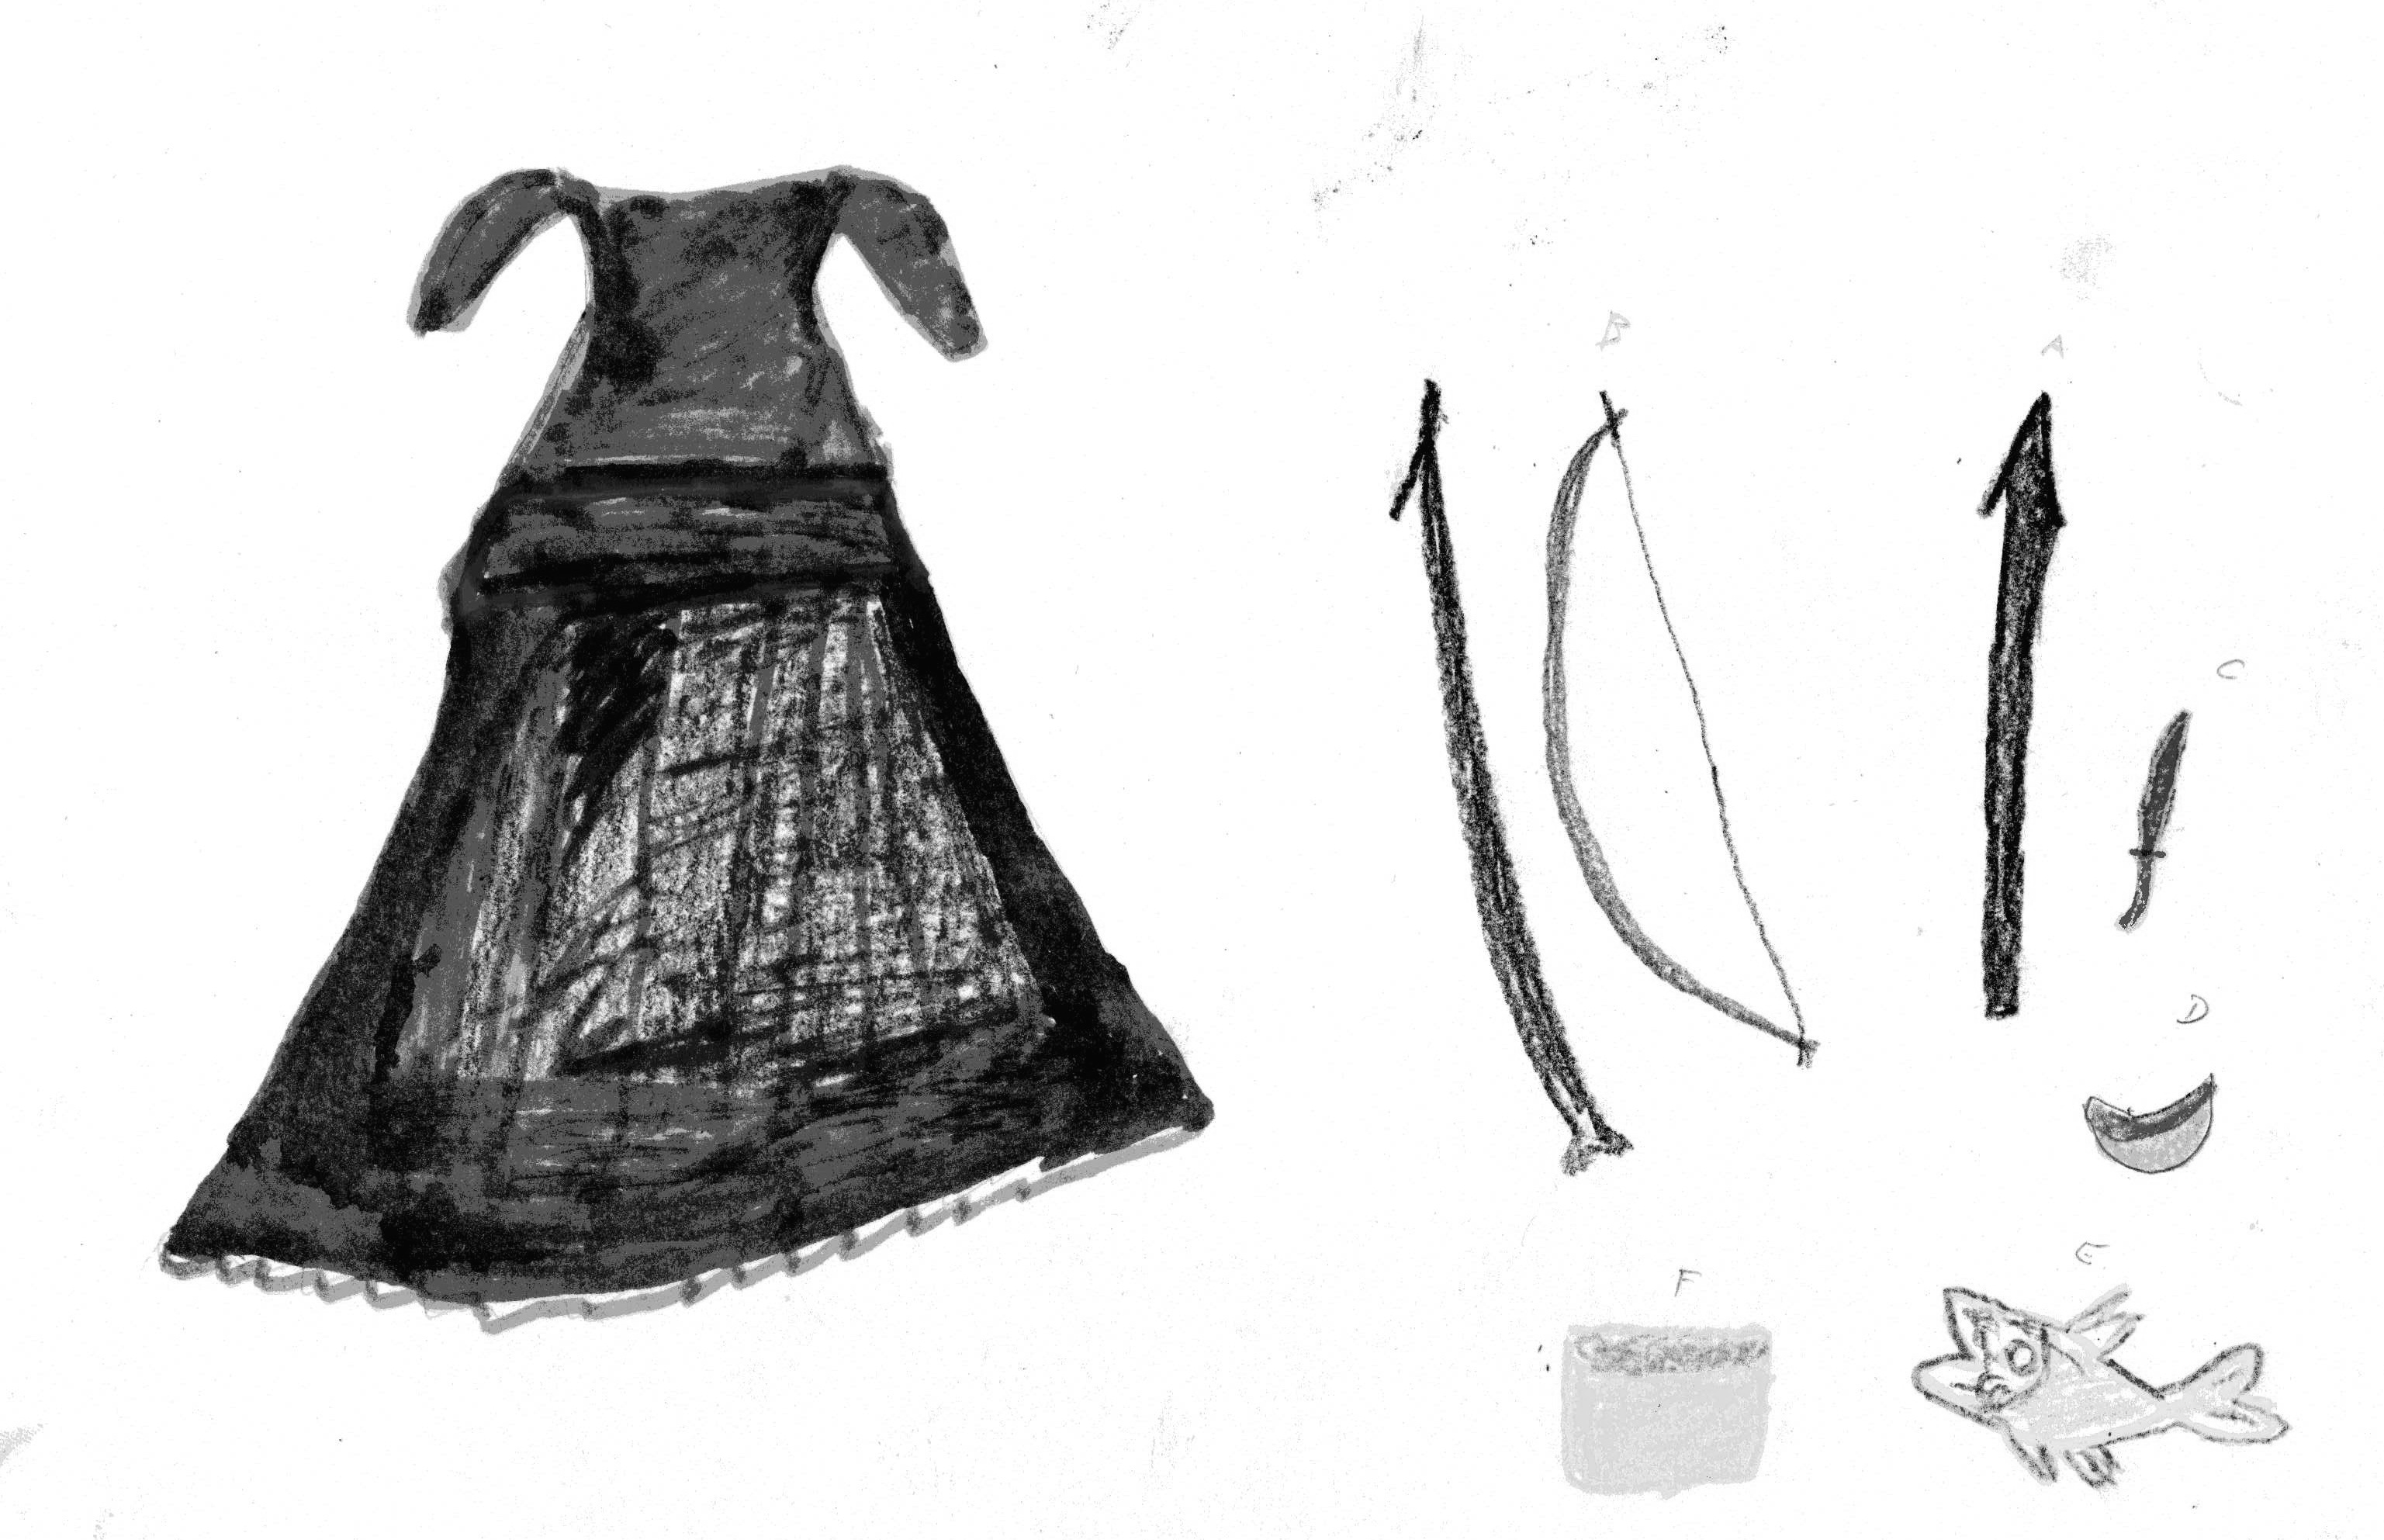
\includegraphics[width=\textwidth]{./img/020}
%\caption{Roupa \textit{Dö̗h Ã̗y}, armas e alimentos (Desenho: M'e̖h Sɨh/Samuel Brasil Monteiro)}
%\end{figure}

A roupa cósmica dessa caçadora de gente hup torna"-se especialmente
interessante, já que se trata de um corpo humano envolto em uma roupa de
branco que dota essa vingadora de atributos comuns à onça e aos
caçadores hup. Os humanos se vestem com roupas de animais para assumir
seus atributos e perspectivas. Os animais despem"-se de seus trajes para
revelar suas essências humanas. O traje feminino sedutor pode ser visto
como uma alta costura capaz de tramar a violência e terror dos brancos
com as linhas de sua corporalidade revestida pelas roupas de pano e pela
predação animalesca. Reid ressalta que os Hupd'äh percebem os brancos
como seres dotados de \textit{forte raiva} como os espíritos da floresta e
como os Tukano. Em suas palavras,

\begin{quote}
Todos eles organizam seus assentamentos a partir de padrões elaborados e
possuem hábitos peculiares como as restrições e os desvios sexuais e
alimentares. {[}\ldots{}{]} Todos eles partilham uma característica que
é particularmente não humana do ponto de vista dos Hupdʉ: possuem \textit{Toew
Pubm} --- forte raiva. {[}\ldots{}{]} A associação que eles fazem entre
raiva e poderes sobrenaturais leva os Hupdʉ a concluírem que os Não
Indígenas possuem considerável poder xamânico. No pensamento dos Hupdʉ
esse ponto é confirmado através da superioridade tecnológica dos Não
Indígenas. Certamente, na região do Uaupés, a superioridade tecnológica
levou primeiramente à dominação política dos Índios do rio e,
posteriormente, dos não Indígenas. A analogia vai mais além, por
equacionar a relação entre poder tecnológico e poder espiritual.
{[}\ldots{}{]} Como essas qualidades são exageradas, os não Indígenas
são vistos mais como espíritos da floresta e como os índios Maku
distantes {[}\ldots{}{]}\footnote{Reid, 1979, p.\,212-3.}
\end{quote}

A tecnologia, os hábitos sexuais e alimentares combinam"-se à raiva e
dotam os brancos de poderes xamânicos e de semelhança com \textit{b'atɨ̖b'},
seres selvagens, e como os Tukano. Esses atributos parecem condensar"-se
no tecido dessa roupa poderosa que faz uma mulher hup, mobilizando
poderes dos brancos, metamorfosear"-se num \textit{espírito da floresta}, uma
predadora voraz em busca de vingança. A roupa, uma arma sedutora,
potencializa sua raiva, sua sexualidade e seu regime alimentar
antropofágico. De modo interessante, essa roupa cósmica converte
características dos brancos em marcas de uma animalidade poderosa. De
forma semelhante, as Onças, que retornam de São Gabriel bebendo cachaça
e disparando suas espingardas-trovões, nutrem"-se da tecnologia, da raiva
e da bebida dos brancos para expressar sua força, violência e seu
domínio.

O xamã vestido de onça e a mulher hup em trajes de \textit{Dö̗h Ã̗y} utilizam o
arco e flecha, a lança e a faca, todas elas armas dos antigos caçadores
e guerreiros hup. Veículos que garantem velocidade e agilidade, essas
roupas cósmicas são também envoltórios de guerra que permitem combater
os inimigos e proteger os animais, de um lado, e os viajantes hup, de
outro. Como uma onça que delimita seu território, mover"-se com essas
roupas auxilia o xamã e \textit{Dö̗h Ã̗y} a cercarem seus domínios no interior
dos quais humanos ou animais podem habitar com segurança. A investida
dos caçadores de jacaré é também um roubo que evidencia a reciprocidade
negativa entre os Hupd'äh e a mulher antropófaga. Diferente do roubo aos
padres e freiras que levam os missionários a se afastarem, a caça causa
a ira desse ente que se aproxima dos Hupd'äh para matá"-los.

\index{af@\textsc{b}5\quad \textit{Ti̖wi̖t hamap bi'i̖d ta'}\break Benzimento dos caminhos}
Retomando \textsc{b5}, a pele da muçurana que reveste os viajantes pode
também ser vista como uma roupa cósmica, não individual, mas coletiva,
uma roupa que é um caminho cercado. Pensando com Deleuze e Guattari,
esse \emph{devir"-muçurana} é uma posição de massa por meio da qual o
sujeito assume uma posição em relação à multiplicidade"-muçurana. Dentro
da muçurana, a maneira como cada pessoa hup liga"-se à \textit{multiplicidade
caminhante} é fundamental para que todos rumem como um \textit{corpo povoado
de multiplicidades}, como uma serpente"-caminho. De forma semelhante, os
viajantes posicionam"-se no interior do território de um xamã"-onça, e
buscam predar os animais situados no domínio de \textit{Dö̗h Ã̗y}. Produzida pelo
benzedor, a pele da muçurana, uma devoradora de jararacas, é uma roupa
para vestir e cercar a multiplicidade, mas é também uma arma móvel, uma
\textit{máquina de guerra nômade} que faz dos andarilhos uma temível serpente
predadora.

\index{13@\textsc{m}4\quad A \textit{Dö̗h Ã̗y} e seu marido}
Os sonhos que Ponciano e Valter tiveram antes de rumarmos para
\textit{D'o̗k"-Paç} e \textit{Ni̗k"-Hũ̗-Paç} foram bons presságios. Para o primeiro, as
moças caminhando para a roça chupavam cana e aceitaram \textit{namorar} com o
velho. Ponciano ria enquanto contava. Chupar cana e aceitar a companhia
de um homem quando se vai à roça surgem como convites para o intercurso
sexual. Em \textsc{s2}\index{bb@\textsc{s}2\quad O sonho de Ponciano}, como em \textsc{m4}, a satisfação alimentar
acompanha a satisfação sexual das moças, e é o senhor hup que aparece
como dotado de um apetite sexual exacerbado, já que acompanha não uma,
mas algumas jovens à roça. Entendendo o intercurso sexual a partir da
caça, pode"-se dizer que Ponciano e Valter se situam na posição de
predadores como \textit{Dö̗h Ã̗y}. De forma parecida, \textit{Tud Asa̗w}, uma moça
ancestral, jogava água e lama nos rapazes para seduzi"-los, sendo, como
\textit{Dö̗h Ã̗y}, uma mulher dotada de um apetite sexual exacerbado. Na análise
de \textsc{m4}, o grito de \textit{Dö̗h Ã̗y}, uma mulher lasciva, evidenciava o
caráter sedutor do chamado aos caçadores"-presas. Desse modo, é possível
dizer que como uma caçadora, \textit{Dö̗h Ã̗y} grita, como uma mulher Branca, ela
veste seu traje de gala para o ataque.
\index{13@\textsc{m}4\quad A \textit{Dö̗h Ã̗y} e seu marido}

Em um artigo de 1998, Descola propõe três modelos para entender a
variação nas atitudes dos caçadores ameríndios quanto à caça. O caso do
povo Desana é tomado pelo antropólogo como compondo um modelo da
reciprocidade regido por um princípio de equivalência entre homens e
animais que fazem parte de um mesmo cosmos. Tomado como um circuito
fechado homeostático, os xamãs negociam com os donos a troca de
\textit{espíritos} humanos por animais, visando sempre ao equilíbrio. Já o
\emph{modelo de predação} teria como exemplo os Jivaro, que não oferecem
nenhuma compensação pela vida da caça, sendo apenas os excessos punidos
pelos donos dos animais. O modelo da dádiva seria aquele em que o
animal, percebido como afim ou consanguíneo, atende voluntariamente ao
pedido do caçador de ceder"-lhe sua roupa (corpo), do qual ele se desfaz
conservando sua alma sem pedir nada em troca. Essa interação ocorreria
principalmente nos Andes centrais do Peru.

Partindo da reflexão de Descola, creio que a caçadora vingativa, dona
dos animais, explicite traços da forma de interação dos viajantes hup
com os animais como situada entre a reciprocidade erótica e a predação.
Os chamados dos caçadores seduzem as prezas, atraindo"-as. A destreza e
ética do caçador envolvem a precisão na flecha ou no golpe mortal
desferido com atenção e silêncio. O momento do ataque aproxima"-se mais
de um confronto em que os homens e os animais revelam suas armas
primordiais, que de um coito, como leva a crer a descrição de
Reichel"-Dolmatoff sobre os Desana. Haja vista a preocupação do caçador,
após o triunfo da batalha, em identificar e retirar as armas originárias
presentes na anatomia dos animais, descritas pela ``linguagem dos
benzimentos'', \textit{bi'i̖d ɨ̗d}. Como será visto mais à frente, da mesma forma
que a onça delimita seu território nas cabeceiras fazendo com que os
animais aumentem populacionalmente, o xamã e os donos dos animais cercam
as Casas"-dos"-Animais para que realizem seus Dabucuris e se reproduzam.
Havendo necessidade, os xamãs abrem essas casas ou conversam com seus
donos, oferecem almas humanas e/\,ou tabaco para que os animais saiam para
a floresta.

As flores amarelas de dança dos rapazes e seus chamados ao longo dos
caminhos explicitam os aspectos sedutores e festivos da caça. Ocultos
pela pele da muçurana e por suas roupas vocais, os caçadores atraem a
presa como se as tirassem para dançar. No momento preciso, revelam suas
armas e surpreendem suas vítimas. Cercar os Dabucuris dos animais
garante a reprodução e o equilíbrio, em termos de reciprocidade. Atacar
depois da sedução garante surpreender o inimigo despreparado para
predá"-lo. O xamã vestido com a roupa de onça ilumina esse princípio de
uma territorialidade que cerca e assegura as viagens e a reprodução. De
modo diferente, a caçadora vestida, uma antropófaga com sede de
vingança, parece cercar os animais para atrair os homens e devorá"-los.
Como o \textit{b'atɨ̖b'}, que atrai as onças e traíras com pacas e minhocas, essa
caçadora seduz com seu vestido e suas criaturas. Já os brancos seduzem
com suas roupas e mercadorias para as regiões ribeirinhas e para São
Gabriel.

De forma parecida, as onças delineiam os contornos de seu território de
vida e de caça. Num caso, a ameaça se faz por uma disputa por presas
entre predadores humanos e felinos numa dada região. No outro, o embate
coloca"-se pelo fato de \textit{Dö̗h Ã̗y} ter se tornado uma dona dos animais,
algo que ocorre após seu casamento com um animal, o Macaco"-da"-Noite,
que, ao contrário de seu marido hup, sacia"-a sexualmente. Vestido com a
roupa de onça"-preta, Armando acompanhava"-nos e nos cercava, como um
benzedor ao criar um círculo de fumaça, movendo"-se como uma onça que nos
inseria dentro de seu território. De forma semelhante, voando de morro
em morro, \textit{Dö̗h Ã̗y} cerca seus protegidos e espera os caçadores.

\section{No caminho da lagarta do
tabaco}\label{no-caminho-da-lagarta-do-tabaco}

\index{af@\textsc{b}5\quad \textit{Ti̖wi̖t hamap bi'i̖d ta'}\break Benzimento dos caminhos}
Retomando \textsc{b5}, os viajantes rumam para as Casas"-de"-Pedra
envoltos na pele da muçurana que é, ela mesma, um caminho, uma canoa e
uma roupa para cercar os andarilhos, metamorfoseando"-os numa predadora
de jararacas. Antes de iniciar"-se a viagem hup, a tartaruga navega em
sua casa"-canoa para a cabeceira e afasta as nuvens à medida que corta a
água com seus remos (\textsc{b3})\index{ad@\textsc{b}3\quad \textit{Sõ̖h ta̗' bi'i̖d}\break Benzimento de cercar a chuva, ou o inverno}. O benzedor lança seu braço como
Moisés. Seu sopro de fumaça faz as nuvens rumarem para a cabeceira
(\textsc{b4})\index{ae@\textsc{b}4\quad \textit{Sõ̖h ta̗' bi'i̖d}\break Benzimento de cercar a chuva, ou o inverno}. Tendo as cabeceiras como pontos de referência, o xamã
imita as ações da tartaruga, do profeta e da muçurana, e cerca os
percursos a partir da Casa"-do"-Trovão para que os viajantes abram os
caminhos que entrelaçam as casas, os mundos e as vidas dos Hupd'äh às de
seus ancestrais.

\index{af@\textsc{b}5\quad \textit{Ti̖wi̖t hamap bi'i̖d ta'}\break Benzimento dos caminhos}
Um dos movimentos importantes do encantamento (\textsc{b5}) vem a ser o
posicionamento do xamã no caminho da lagarta da folha do tabaco. Ele
entra na comunidade dos filhos da lagarta pequena por sobre seu banco de
leite, segurando seu pedaço de tabaco. Uma vez dentro dessa morada, ele
assume a postura ereta e, a partir daí, transforma seu corpo naquele do
muçum, do calango e do curió, respectivamente, um peixe"-cobra, um
lagarto e uma ave, todos pequenos e capazes de deslocar"-se pela água
(muçum), pelo ar (curió), pela terra (calango) e dentro da terra
(muçum). Dado o tamanho e a agilidade, nutrir"-se com as faculdades
corporais e motoras desses seres garante ao xamã transitar oculto pelas
casas situadas nos vários ambientes, como os viajantes em pele de
muçurana. É a incursão pelo caminho da lagarta do tabaco e à comunidade
de seus filhos o que permite tais metamorfoses corporais e a mobilização
dos animais auxiliares. Esse ente, que habita a planta de tabaco,
torna"-se especialmente relevante para o xamã, pois é capaz de fabricar
um casulo, sua \textit{rede}, fazer crescer suas asas, virar mariposa e voar.
Como observa Reid, a habilidade de transformação de espécies de
mariposas, morcegos, cobras e onças leva os Hupd'äh a vê"-los mais como
\textit{espíritos} do que como animais.

As mariposas (\emph{Manduca quinquemaculata}) procuram as
folhas de tabaco para desovarem e são, ao mesmo tempo, importantes
polinizadoras que auxiliam na reprodução das plantas de tabaco. As
larvas alimentam"-se do tecido vegetal e tornam"-se lagartas que,
posteriormente, comporão seu casulo para a metamorfose e o voo. A planta
de tabaco é o \textit{caminho} ao longo do qual as lagartas se deslocam, o
\textit{alimento} que as nutre a partir das folhas e a \textit{aldeia} onde os
\textit{filhos} nascem e se desenvolvem. Em \textsc{b1}\index{ab@\textsc{b}1\quad \textit{Pũ'ũ̖k bi'i̖d}\break Benzimento da coca}, o benzedor busca
interromper a identificação entre o comedor de coca e a lagarta da coca,
que oferece seu \textit{caarpi} enlouquecedor, passa o dia todo em sua rede e,
devorando a coca, preda uma essência vital humana. Por outro lado, a
mariposa, que se desloca de planta em planta e dá o tabaco, a vida e os
caminhos a seus filhos, pode ser vista como um ser análogo aos xamãs
que, de aldeia em aldeia, de casa em casa, pacificam os inimigos,
mobilizam os animais auxiliares e dão tabaco a seus filhos para que
cresçam sem doenças (\textsc{b2}).\index{ac@\textsc{b}2\quad \textit{Hũ̖t bi'i̖d}\break Benzimento do tabaco}

Abrindo os caminhos antigos com os jovens viajantes, os mentores
conduziam"-nos de morro em morro, de morada antiga em morada antiga,
integrando"-os em uma região de memórias e afetos que, a todo instante,
fazia emergir gostos, palavas e paisagens da infância e juventude de
nossos guias, dos tempos de Semente de Tabaco e dos missionários. As
visitas às Casas"-de"-Pedra inseriam"-nos numa forma específica de
interação, um modo de coabitar com Semente de Tabaco, seguir seus
rastros, imitar seus gestos e encontrar os ancestrais. As águas das
nascentes e os vômitos purificam o corpo para nutrir o pensamento a
partir dessas \textit{rodas de coca oníricas}. A interação \textit{dentro da
caverna} potencializa as rodas de coca \textit{fora da caverna} e assegura a
eficácia da proteção e da cura agenciadas pelos xamãs. Entre o interior
e o exterior das Casas"-de"-Pedra, diversas multiplicidades coexistem,
penetram"-se e mudam de lugar.

Depois que saiu de \textit{Pi̖j"-Dëh}, o pai de Ponciano foi primeiro para
\textit{Ya̖k"-Dëh"-Mo̖y"-Hö̖d}, contou o mentor em nosso percurso a \textit{Hõpoy"-Paç}. De
lá, seguiu para \textit{Pë̖d"-Dëh"-Mo̖y"-Hö̖d} e, depois, para \textit{Wõhoy"-Dëh}. De
\textit{Wõhoy"-Dëh"-K'et"-Yoh}, ele mudou"-se para \textit{Ta̗t"-Dëh}. Em sua vida, seu pai
foi fazendo um percurso semelhante ao do ancestral \textit{Ya̖k} que, vindo de
\textit{Pi̖j"-Dëh}, fez sua casa em \textit{Ya̖k"-Dëh"-K'et"-Yoh}, mudou"-se para
\textit{Wõhoy"-Dëh}, mas, por fim, habitou a região distante do Iraiti. O
ancestral foi voando com sua \textit{wayrö̖'"-tëg}, seu cocar de voar, de um
local a outro. Quando vinha com o pai trabalhar a roça, comiam nas
grutas do morro. ``Meu pai mudou"-se muito de comunidade. Acho que o
próximo lugar onde vão morar é São Gabriel'', concluiu. Iniciando sua
jornada próximo à cabeceira de \textit{Pi̖j"-Dëh}, Serra Grande, a extensão
do deslocamento do ancestral \textit{Ya̖k} atinge a distante terra do Irati.
Ressalta, talvez, quão imensa poderia ser a amplitude da região de
mobilidade dos grupos hup.

Os atos de relembrar de Ponciano e José iam constituindo nossos
percursos de observação como caminhos vividos que mesclavam nossos
movimentos àqueles dos ancestrais. Os caminhos antigos, as
Casas"-de"-Pedra e as Moradas Antigas parecem apontar, como já afirmava
Reid, para uma existência social e convívio de longa duração nessas
regiões. Há semelhança entre os itinerários dos ancestrais e aqueles dos
pais e avós dos viajantes hup. A identificação de tantos assentamentos,
lugares sagrados, artefatos, a reabertura de caminhos antigos, com as
descrições das práticas rituais nas Casas"-de"-Pedra, revela as cabeceiras
como sendo pontos de referência para os padrões de mobilidade hup. Os
caminhos dos antigos eram também os caminhos dos ancestrais que mudavam
periodicamente suas moradas dos arredores de um morro ao outro.
Concentrando"-se na região dos morros até a década de 1950, os antigos
Hupd'äh repisavam cotidianamente os caminhos dos \textit{primeiros Hupd'äh}.

Com base no estudo de toponímias e nas observações de viagem,
Koch"-Grünberg propõe que os Maku, inclusos os Hupd'äh, seriam os
descendentes de antigas tribos que teriam povoado o Uaupés e depois sido
comprimidos e fusionados pelos Aruaque e Tukano (Betoya), vindos do
oeste e sudoeste. Mais tarde, Nimuendajú revalida tal hipótese afirmando
a vida errante dos Maku que, desconhecendo a cerâmica, a lavoura, a arte
têxtil e as habitações permanentes, seriam populações de cultura
rudimentar que habitam os centros da mata. O afastamento para as
cabeceiras, ocasionado pela ocupação territorial tukana é afirmado por
Bruzzi Alves da Silva, e figura, na visão de Métraux, como um
deslocamento populacional face ao contato com os não indígenas, que
teria resultado numa cultura decadente de grupos Maku"-Nômades,
descendentes de antigos Maku ribeirinhos e agricultores. Por fim, Reid
toma como referência as narrativas hup para dizer que os Hupd'äh teriam
vindo do leste e chegado àquela região. Seus ancestrais tinham na caça e
na coleta suas atividades principais. O afastamento extremo para as
cabeceiras foi simultâneo ao avanço da empresa da borracha, sendo a
agência missionária um fator crucial para a fixação recente dos grupos
hup nas grandes aldeias ribeirinhas.

Ainda que tenham habitado as áreas ribeirinhas, penso que a sucessão de
assentamentos nessa região das cabeceiras a situe como um \emph{centro
nodal} a partir do qual os diversos grupos hup, ancestrais aos grupos
regionais de \textit{Ta̗t"-Dëh} e \textit{Pi̖j"-Dëh}, tenham mudado suas moradas ao longo
de um grande intervalo de tempo. O \emph{afastamento para as cabeceiras}
pode ser visto, alternativamente, como uma \emph{aproximação às
cabeceiras}, durante dados períodos, uma aproximação a esses centros do
mundo que parecem não ser nada estranhos nem aos senhores hup e nem aos
seus antepassados mais distantes.

Percorríamos caminhos que, ao levarem os Hupd'äh de uma Casa"-de"-Pedra à
outra, os conduziram também de uma aldeia a outra, como ocorre com os
voos das mariposas de tabaco. Viajando para as cabeceiras, os antigos
movimentavam"-se como Semente de Tabaco, Arara e outros tantos ancestrais
que passaram por aquelas searas e, por vezes, ainda retornam a suas
habitações ctônicas. Tomando as cabeceiras, e não os grandes rios, como
pontos de partida para observar os movimentos dos grupos populacionais
hup, deixam"-se de ter grupos hup \textit{pressionados} ou \textit{refugiados} face
ao inexorável avanço dos Tukano e Aruaque, ou dos brancos. Há, sim,
grupos hup que se aproximam desses centros e meios progenerativos para, a
partir deles, lançar seus paris e interagir com esses Outros que são
Onças, Trovão, jararacas, Tukano, brancos, \textit{Dö̗h Ã̗y}, vestidos e armados
para trocas e combates, para a reciprocidade e para a predação.

É no percurso entre as rodas de coca, os caminhos e as Casas"-de"-Pedra,
movendo"-se como pessoa"-corporificada, como pessoa"-sopro ou como
pessoa"-onça vestida, que múltiplas condensações rituais ocorrem a partir
do modo como os viajantes se posicionam num campo de rastros deixados
pelos ancestrais, presas, feras, brancos, etc. Tomando as palavras de
Deleuze e Guattari,

\begin{quote}
De um lado, as multiplicidades extensivas, divisíveis e molares;
unificáveis, totalizáveis, organizáveis; conscientes e pré"-conscientes
--- e, de outro, as multiplicidades libidinais inconscientes,
moleculares, intensivas, constituídas de partículas que não se dividem
sem mudar de natureza, distâncias que não variam sem entrar em outra
multiplicidade, que não param de fazer"-se e desfazer"-se, comunicando,
passando umas nas outras no interior de um limiar, ou além ou aquém. Os
elementos destas últimas multiplicidades são partículas; suas
correlações são distâncias; seus movimentos são brownoides; sua
quantidade são intensidades, são diferenças de intensidade.\footnote{1995,
p.\,60.}
\end{quote}

Descrevendo a estrutura das rodas de coca, foi possível entender como a
interação entre dono e apanhador situa ritualmente diferenças de clãs e de
domínio territorial. Ao mesmo tempo, os comedores de coca devoram a
carne e o osso do Velho Cobra e repetem os atos ancestrais de Semente de
Tabaco. Simultaneamente, a esse \textit{modo molar} de unificar, centralizar
e organizar essa forma relacional de interação, as palavras, os
deslocamentos oníricos aliam"-se às andanças pelos caminhos e aos vômitos
nos \textit{ho̗n hö̖d} para explicitar esse longo processo ritual composto por
linhas de fuga, itinerários que situam formas de desterritorialização, e
permitem ver a matriz dessas ações ritualizadas não apenas como centros,
mas também como meios de \emph{progeneração} da vida. Situando suas
percepções e ações ao longo de um campo complexo de ações ritualizadas
convergentes, de campos de rastros, os sujeitos guiam"-se por direções
movediças entre a aldeia, o caminho e o morro; nem sedentários nem
nômades, e muito menos seminômades, os viajantes caminham por paisagens
selvagens, ctônicas, lácteas, celestes que os levam ao encontro de
ancestrais, feras, vingadores antropófagos, tartarugas e profetas. As
Casas"-de"-Pedra são assim centros e meios de \emph{progeneração} da vida,
que posicionam os benzedores dentro de uma Casa"-do"-Trovão às margens do
Lago de Leite. De lá, os viajantes aprendem a lançar seus paris e a
transformar todos os caminhos em Rios de Leite para a navegação numa
Cobra"-Canoa que os leva aos morros e à cidade de São Gabriel.


\chapter{Lagos de leite}\label{lagos-de-leite}

\setlength{\epigraphwidth}{.60\textwidth}
\begin{epigraphs} 
\qitem{Que nada,\\
Minha porção mulher que até então se resguardara\\
É a porção melhor que trago em mim agora,\\
É o que me faz viver.}{\textsc{gilberto gil}}
\end{epigraphs}

\section{\textit{Bisi̗w} e a Casa"-dos"-Animais}\label{bisiw-e-a-casa-dos-animais}

O chão ressoa a cada passo. Dentro da Casa"-dos"-Animais, a superfície
rochosa reveste o interior oco do morro. O granito reverbera os
movimentos dos visitantes. Os ecos convidam os animais a deixar a
habitação ctônica para, livres, percorrerem as matas. Mas a morada
acústica denuncia a chegada de intrusos ao dono dos animais. Por isso,
todo cuidado é pouco. O \textit{Bisi̗w}, irmão maligno de \textit{W'ed B'ö̖'}, pode
surgir a qualquer momento e aniquilar os viajantes.

Era para essa caverna que antigos xamãs, benzedores e pajés, rumavam
quando a escassez das presas fazia a fome assolar as aldeias. No
interior é possível ver ainda a grande pedra sobre a qual era aberta uma
folha de bananeira. Um dos viajantes, munido com um bastão, arremessava
sua arma com toda força contra o tecido rochoso. O estrondo penetrava o
morro com seus ecos ordenando aos animais que abandonassem sua morada e
ascendessem para a superfície terrestre.

Naquela manhã, quando chegamos à \textit{Hu̗͂-Mo̖y}, a Casa"-dos"-Animais,
Ponciano fez questão de demonstrar esse \emph{chamado aos
animais},\footnote{A comparação da percussão ritual ao chamado sedutor da
  caça pelos assobios, como visto no capítulo \emph{Viagem à Serra Grande}, permite perceber a
  batida na pedra como uma caça de batuque, algo próximo à análise de
  Lévi"-Strauss para os Tupi"-Kawahib (2004b, p.\,287).} batendo forte com
uma vara na pedra. Entretanto, disse não ser mais possível fazer com que
as presas saiam para a floresta dessa forma. Uma grande cerca, criada
por feiticeiros inimigos, obstrui completamente a passagem. É por isso
que as caças diminuíram tanto na região nos últimos tempos. Viajando
oniricamente e penetrando o interior da Casa"-dos"-Animais, Ponciano e o
pajé Armando viram essa barreira intransponível. Por vezes, o \textit{sä̗w},
``pajé'', cheira paricá, ruma como pessoa"-sopro até a morada dos
animais e encontra o \textit{Bisi̗w}. Conversando diplomaticamente, procura
fazê"-lo liberar presas para circularem pelas matas. Como descreve Reid,

\begin{quote}
Pensa"-se que essas \textit{casas} são subterrâneas, com acesso ao chão da
floresta através de buracos e cavernas. Diz"-se que cada uma dessas casas
é muito semelhante a este Mundo superior, têm suas próprias malocas,
plantações, igarapés e florestas, etc. Cada um deles é controlado por um
\textit{Nyo'om I} {[}\ldots{}{]} um ``mestre''. Alguns desses mestres espirituais
possuem uma existência solitária, como é o caso de Dohai {[}\ldots{}{]}.
Outros são mestres das \textit{casas dos animais}, {[}\ldots{}{]} e possuem
um papel importante no controle de todas as espécias de caça e dos
animais em geral. Além desses mestres dos animais generalizados, há
casas florestais controladas por mestres espirituais de cada espécie de
animal em particular. Embora os Hupdʉ sejam cientes de que os animas se
reproduzem nessa Terra, eles também acreditam que alguns mestres de
espécies criam"-nos em suas casas subterrâneas. {[}\ldots{}{]} De tempos
em tempo, quando a caça se torna escassa, os xamãs podem entrar em
contato com esses mestres espirituais e pedir"-lhes que liberem mais
animais para a floresta. Alguns Hupdʉ afirmaram que essas transações
envolvem o pagamento da liberação de caça com almas humanas, enquanto
outros disseram que os xamãs oferecem dádivas de fumaça de tabaco apenas
aos mestres espirituais.\footnote{Reid, 1979, p.\,261.}
\end{quote}

Desse modo, a caverna dá acesso a um mundo subterrâneo pleno de malocas,
roças e igarapés onde, sob o granito das rochas, diversos tipos de
animais vivem, trabalham e praticam seus rituais. Dono dos animais,
\textit{Bisi̗w} parece ter um papel importante na reprodução desses seres que,
atendendo a seus desígnios, abandonam a vida subterrânea e passam a
habitar a planície florestal. Como a coca que acalma a fúria do Trovão,
a troca com \textit{Bisi̗w} se estabelece por meio do oferecimento alimentar
quer de tabaco, um óleo para temperar sua coca, quer de \textit{espíritos}
humanos, entre os quais inimigos tukano ou pessoas hup de outros grupos
locais mortos com feitiços soprados pelos xamãs hup. A viagem onírica do
pajé e a viagem dos antigos benzedores revelam"-se sequências de ações
ritualizadas que, pelo uso da palavra e do estrondo percussivo, marcam
formas de interação com esse perigoso dono que cria e liberta animais,
ao mesmo tempo em que devora e aniquila seres humanos.

Foi em meio a nossa incursão à Casa"-dos"-Animais que vi pela primeira vez
as lascas de cerâmica espalhadas pelo chão. Os restos das cuias de
Semente de Tabaco estavam próximos à pedra percussiva. Ponciano explicou
que aquele morro tinha sido habitado pelo ancestral \textit{Hu̖͂t"-Wäg} antes da
chegada de \textit{Bisi̗w} e as Onças. Para fazerem \textit{b'ok"-ka̗b b'a̗h},
``recipientes de cerâmica'', os antigos queimavam o barro misturado com
um pouco de madeira. As lascas no chão remetiam, assim, à criação da
humanidade e manifestavam a presença desse ancestral, mestre dos
encantamentos e narrativas míticas, fundamentais para a proteção, cura e
crescimento das pessoas hup a partir de seus ouvidos e de seus sopros
vitais. A chegada de \textit{Bisi̗w} e das Onças marca a perda de domínio dos
ancestrais hup sobre essa morada e, desse modo, sobre o controle da
procriação e dispersão das presas.

Perto da Casa"-dos"-Animais havia também uma \textit{Ho̖͂p"-Mo̖y},
Casa"-dos"-Peixes, um grande lago que é uma aldeia dos peixes. ``É por
isso que os igarapés daqui têm muitos peixes'', disse Ponciano. Partindo
desse grande lago, os peixes descem os igarapés e chegam ao curso dos
rios. Ao descrever a importância dos morros para os Desana,
Reichel"-Dolmatoff diz que:

\begin{quote}
As grandes serras rochosas que se elevam isoladamente na floresta são
úteros onde vivem os animais silvestres e os poços profundos nas
corredeiras são úteros subaquáticos onde moram os peixes. Os ninhos
suspensos de certas aves como o papa"-figo e o gaio (ambos
\emph{Icteridae}), se comparam com o útero, sendo o mesmo para os ninhos
de colibris e periquitos (\emph{Psittacidae}) que se aninham nas árvores
ocas.\footnote{Reichel"-Domatoff, 1986, p.\,8-88.}
\end{quote}

\textit{Hu̗͂-Mo̖y k'ö̗d dä̗b pä̗' ni̗i̗!}, ``Dentro da Casa"-dos"-Animais há muito
Dabucuri!'', foi o modo como Ponciano descreveu a vida plena de festas e
cópulas das presas no interior do morro. À luz do comentário de
Reichel"-Dolmatoff, creio que também para os Hupd'äh esse morro oco possa
ser tomado como um útero ctônico. Cercada por feiticeiros inimigos, essa
casa passou a ser um útero fechado que fez com que os moradores da
região passassem a caçar cada vez menos. A pesca, tida como abundante ou
suficiente em alguns igarapés, foi tornando"-se cada vez mais a atividade
diária de trabalho masculina. \textit{Hu̗͂ me̗h}, ``caçar'', é hoje uma atividade
esporádica e que encontra nas lembranças dos velhos a nostalgia dos
tempos em que se comia muita carne.

Antes de chegarmos a esse nosso destino, paramos, e Ponciano acendeu um
cigarro. Sopramos a fumaça em nossos corpos. Esse era um \textit{ti̖wi̖t ha̗ma̗p
bi'i̖d ta̗'}, um ``benzimento dos caminhos'', preparado especificamente
para proteger"-nos dos \textit{Tëg D'u̗h Hup}, as Gentes"-Árvore, cuja aldeia,
sua Casa"-da"-Mata, está sediada próxima dali. Como visto em
\textsc{b5}\index{af@\textsc{b}5\quad \textit{Ti̖wi̖t hamap bi'i̖d ta'}\break Benzimento dos caminhos}, as perigosas Gentes"-Árvore precisam ser afastadas dos
caminhos. Tal qual as Cobras, as Gentes"-Árvore podem atingir os
viajantes com seu ``bastão'', \textit{kötö̖w"-tëg}, e causar a terrível ``dor de
carne'', \textit{kɨ͂kɨ̗͂nɨ̗͂}. Por isso é preciso fazer com que larguem seu pedaço
de tabaco e seus bastões de embaúba"-\textit{sãy} e de embaúba"-\textit{wa̗g} sobre o
jirau dentro de suas casas. Se com bastões os antigos causavam o
estrondo que abria o morro, com bastões as Gentes"-Árvore são capazes de
ferir e impedir a continuidade das viagens, protegendo assim sua morada
dos intrusos.

Ora para alertar"-nos, ora para ensinar"-nos, nosso mentor não cansava de
indicar árvores e arbustos durante o trajeto. Foi assim que conheci o
\textit{sarah"-s'o̖m}, planta cuja casca era usada para limpar o corpo durante o
banho: \textit{wähä̗d nɨ̖h sabaw}, ``o sabão dos antigos'', ria Ponciano.
Provei as frutas da árvore \textit{heb a̗g}, de sabor muito doce, ideais para
nossa merenda. Esfregando uma folha no rosto, o jovem Ari ensinou"-me que
a \textit{we̖g k'et} era a folhagem com a qual os antigos hup limpavam o rosto.
Batendo a mão contra o tronco de uma árvore, Ponciano mostrou"-me a
\textit{pe̗͂y"-tëg}, ``pau"-d'arco'',\footnote{\textit{pe͂y"-tëg}, pau"-d'arco (\emph{Tabebuia
  sp.}), nome dado a várias espécies de árvores usadas para fazer arcos.
  Família das bignoniáceas. Cf. Ramirez (2006).} madeira extremamente
dura e boa para a fabricação de arcos. A interação com as árvores e com
as Gentes"-Árvore fazia"-se fundamental nesse nosso percurso de
observação, possibilitando atos de rememoração e proteção que iam
garantindo nosso deslocamento por aquelas paragens. Muito atentos, Ari e
eu observávamos cada detalhe daquele universo que se constituía, pouco a
pouco, como uma vasta região trazida à vida pela confluência dos
percursos dos movimentos de humanos, animais e espíritos.

%\begin{figure}
%\centering
%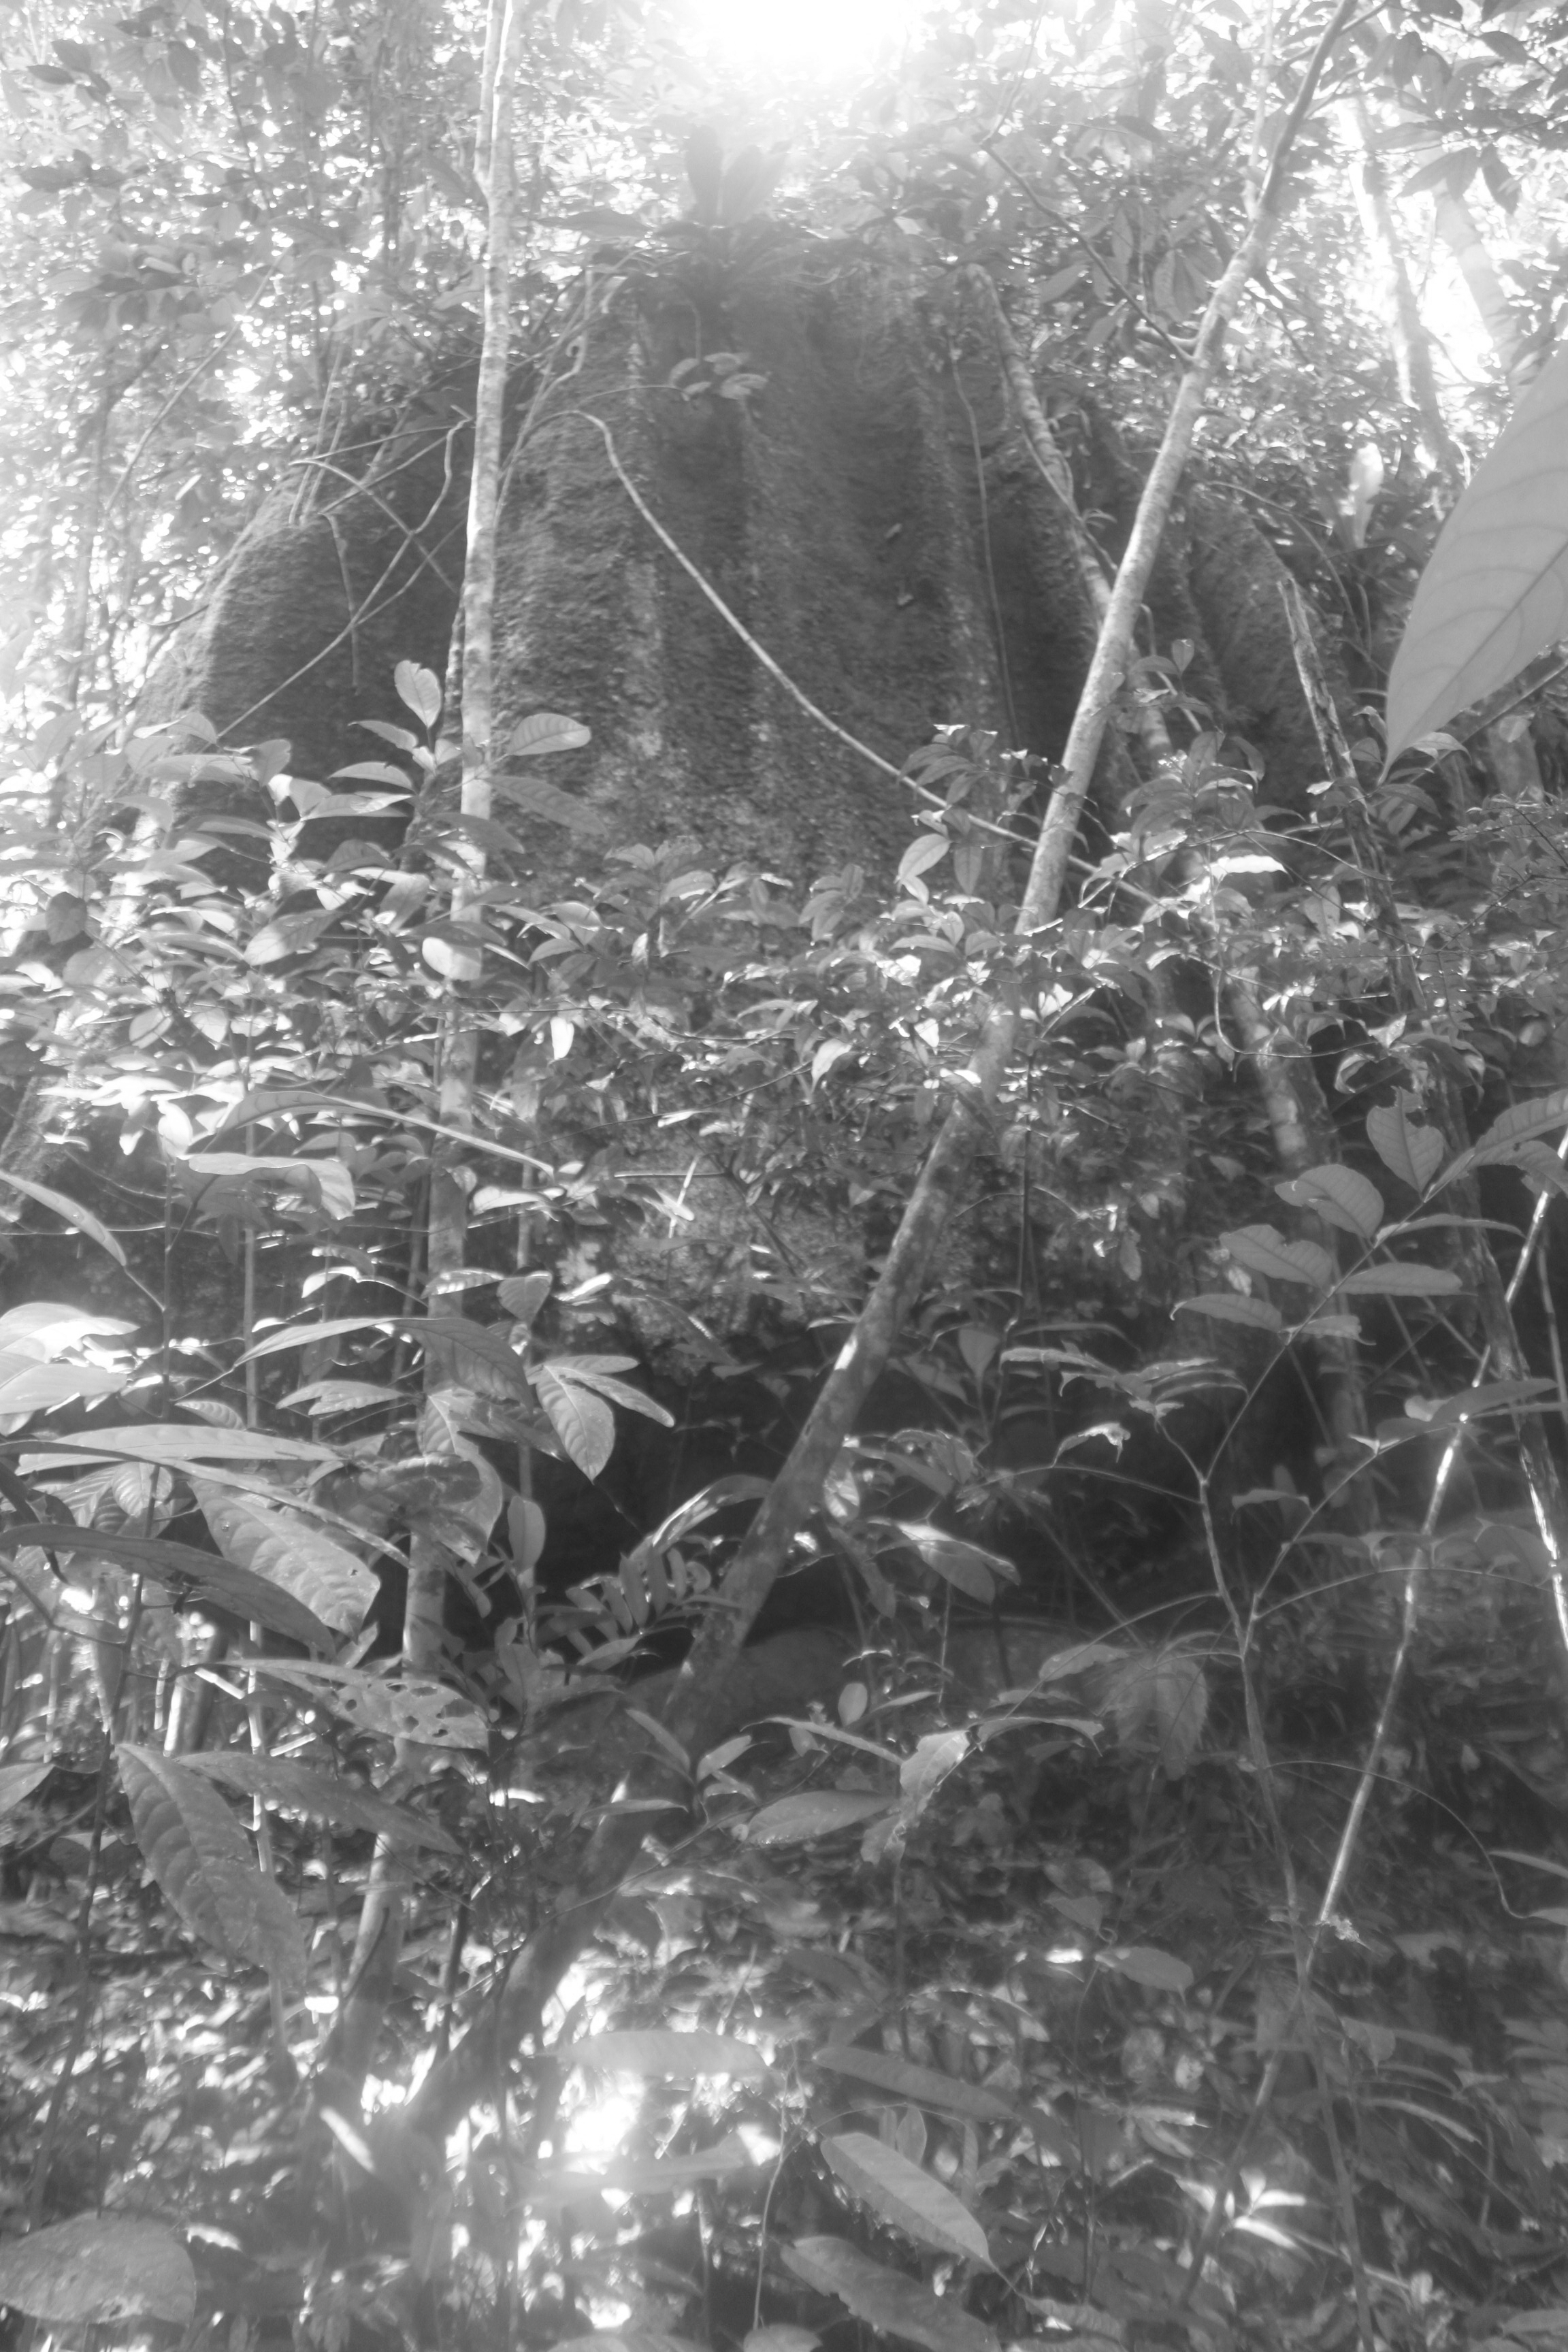
\includegraphics[width=\textwidth]{./img/021}
%\caption{Vista externa da Casa"-dos"-Animais (foto: Danilo P. Ramos, 2012)}
%\end{figure}

Na volta, quando já estávamos cruzando as roças da comunidade, Ponciano
ouviu o som de um macaco. Percebendo o balanço das folhagens próximas,
Ari começou a procurá"-lo. Tinha seu arco e flecha preparado. Imitava com
a boca o som do animal para atraí"-lo, enquanto aproximava"-se
vagarosamente. Num instante, soltou suas armas e trepou nos galhos. Logo
conseguiu agarrar o bicho que, na realidade, era um pequeno filhote
assustado. Ponciano disse que o levaríamos conosco para que seus netos
brincassem com ele.

Cansados da caminhada, fomos para a roda de coca logo que chegamos à
aldeia. Já sentados ou preparando o alimento da origem, os senhores
interromperam seus afazeres para ver as fotos que tiramos da
Casa"-dos"-Animais. ``Os veios das paredes são teias de jararaca'',
comentou Luis. ``Os antigos batiam na pedra e os animais saíam'',
continuou. As crianças que brincavam perto da roda amontoaram"-se em
torno de nós. Arregalavam os olhos para ver as fotos e ouviam
atentamente as histórias de \textit{Bisi̗w} que Ponciano começava a contar. É
sempre com muito medo que os pequenos ouvem sobre o \textit{Bisi̗w}, pois esse
ancestral é um abominável devorador de rapazes. As histórias que ouvi de
Ponciano e Jovino em encontros noturnos em 2011 são correntemente
narradas pelos avós a seus netos. Acredito que as versões abaixo
permitam entender melhor esse mal estar com que os menores ouvem sobre
esse dono dos animais.

\begin{quote}\index{24@\textsc{m}15\quad \textit{Bisi̗w}, o devorador de rapazes}
\mito{15}{\textit{bisi̗w}, o devorador de rapazes}

O \textit{Bisi̗w} deu as flautas. Primeiro ele era igual a uma pessoa. O som
dele zoava o som do Jurupari, da \textit{tã'ã̗y}, ``fêmea'', e do \textit{tiyi̖'},
``macho''. O \textit{Bisi̗w} transformou"-se num toco onde os meninos entraram.
Eles estavam imitando o som dele. Ele mostrou"-lhes o corpo e seu som
zoando. Falou para os rapazes fazerem uma festa para ele.

Cada povo conta o seu. A outra história começa assim, outra história ele
vem na origem. Cada grupo vinha com a sua história. Para nós, o \textit{Bisi̗w}
era forma de pessoa. Ele e \textit{We̗d B'ö̖'} são gêmeos e \textit{Bisi̗w} é \textit{pu̗y'},
``irmão menor''. Primeiro, ele tinha forma de gente, o corpo zoava.

Os meninos estavam imitando, ele mostrou como zoava o corpo. Pediu para
as crianças fazerem Dabucuri. O \textit{Bisi̗w} subiu na árvore de uacu e pediu
para os rapazes não saírem debaixo do pé. As crianças assaram o caroço
de uacu e a fumaça chegou para ele. Ele desmaiou. Depois, disse: ``Vocês
também vão sentir como eu senti''. Aí, ele fez uma chuva. Transformou"-se
em toco e os rapazes entraram dentro dele. (Entraram pelo seu ânus). Ele
comeu todos os meninos. Um escapou, comeu uacu e foi avisar os pais. Os
pais estavam querendo matá"-lo, e não conseguiram. Ele foi para a
\textit{Paç"-Mo̖y}, Casa"-de"-Pedra.

O pai do rapaz mandou preparar bebidas e falou para o pássaro \textit{weyt},
``periquito'', para avisar o \textit{Bisi̗w}. O pássaro foi e começou a dizer a
ele quais os tipos de bebida os homens tinham preparado. O \textit{Bisi̗w} não
queria aceitar, mas aceitou ir beber uma \textit{sawi̗h dëh},\footnote{\textit{sawi
  tëg}, ``pau amarelo'', árvore da família das rutáceas,
  \emph{Euxylophora sp.} Cf. Ramirez (2006). É uma árvore de terra firme
  que possui flores amareladas, aromáticas, frutos capsulares e uma
  madeira boa para artesanato (Silva, M.; Lisbôa, P.; Lisbôa, R., 1977).}
``caxiri da fruta de pau amarelo''. Então, ele foi até a casa dos pais
para beber. Deixaram uma panela de caxiri para oferecer a ele. A panela
era de barro como faziam antes, uma \textit{b'ok"-tä̗w}. Deixaram essa panela
para oferecer só para ele, pois o caxiri estava benzido para que ele
logo se embriagasse. \textit{Bisi̗w} falou: ``Vocês querem vingança!'' Eles
foram pegar lenha e fogo. Empurraram"-no. Ele queimou. Antes tinha dito:
``Vocês vão cortar lenha, vão me queimar e vão sentir o que eu senti.
Vocês vão brigar, vão matar, vão envenenar''. Foi aí que começou o corpo
dele desse jeito. Com esse fogo que queimaram o corpo dele é que
apareceram as flautas.

Foi \textit{K'e̖g Te͂h} quem pegou as flautas e entregou para cada grupo no Lago
de Leite. Do corpo queimado dele surgiram as flautas, muitas. Outros
grupos podem contar mais, saber mais, mas a gente conta assim. \textit{K'e̖g
Te͂h} encontrou o \textit{Bisi̗w} queimado e levou as flautas para o Lago de
Leite para dar à humanidade. As flautas eram os ossos de \textit{Bisi̗w}. Do
Lago de Leite a humanidade veio embaixo d'água na \textit{M'e̖h"-Hoh"-Të̖g}, a
Cobra"-Canoa, até Ipanoré, \textit{Hib'a̗h"-Höd}. Então, desceram de novo
até o Lago de Leite e subiram de novo, invisíveis. Foi aí que \textit{K'e̖g Te͂h}
entregou para cada grupo as flautas. Aí, a humanidade teve cada um a sua
flauta. Já subiram com a flauta na canoa. Essa transformação da canoa
foi em Ipanoré. Subiram todos os rios: Uaupés, Papuri, Tiquié. Subiram
de canoa e vieram todos se encontrar nessa Serra da
Menstruação, da Iniciação ou do Pedaço, \textit{Te͂h"-S'ɨ̗g"-Mo̖y"-Paç}. Saíram de canoa em
Ipanoré e, andando, atravessaram em São Tomé, perto de Boca da Estrada.
Lá tem a pedra onde eles atravessaram. Foram se encontrar nessa Serra da
Iniciação e daí mostraram o que receberam.

Nessa ``morada'', \textit{Mo̖y}, havia três casas. A primeira só tinha banco
para sentar. A segunda era a casa dos homens com as flautas. A terceira,
eles cercaram com pari para as mulheres ficarem dentro e não verem as
flautas. Na segunda casa é que mostraram, entre os cunhados, o que
receberam. Como agora que se faz a coca entre cunhados. Aí mostraram
cada flauta. Todos os grupos foram mostrando e tocando até o final. Foi
então que cada grupo se espalhou. Estavam lá os Tukano, os Desano.\footnote{Jovino, gravação sonora, 24 de agosto de 2011.}
\end{quote}

\begin{quote}\index{25@\textsc{m}16\quad A gestante tapada}
\mito{16}{a gestante tapada}

Primeiro, nasceram os dois filhos. O \textit{Bisi̗w} nasceu e o outro menino.
Eram dois dentro da barriga, dizem. Já estava na hora de receber, de
saírem os filhos, mas ela não tinha ânus (nem vagina). A mãe não tinha
ânus e já estava na hora de receber e saírem (os filhos). Foi um
ancestral que fez o ânus para ela.

Ele acompanhou e benzeu na hora de nascer o \textit{Bisi̗w} e o \textit{Wed B'ö̖'}. Fez
o ânus para ela e depois se diz que a mãe não sabia. Ela esqueceu (que
antes não tinha nem ânus nem vagina).

Naquele lugar, ela teve o \textit{Bisi̗w} e o \textit{Wed B'ö̖'}. (O pai tirou os dois
filhos, mas deu só \textit{W'ed B'ö̖'}.) Tirou os dois, mas escondeu um
(\textit{Bisi̗w}). Entregou somente \textit{Wed B'ö̖'} para a mãe. Então, ele cresceu
(ficou rapaz) sem mãe.

Dizem que morava só \textit{We̖d B'ö̖'} e a mãe. Aquele que não teve mãe ficava
sozinho (sem mulher), diz"-se.\footnote{Ponciano, gravação sonora e tradução,
4 de julho de 2011.}
\end{quote}

\index{25@\textsc{m}16\quad A gestante tapada}
\index{24@\textsc{m}15\quad \textit{Bisi̗w}, o devorador de rapazes}
Essas duas passagens da história dos gêmeos \textit{Wed B'ö̖'} e \textit{Bisi̗w} foram
contadas por Jovino (\textsc{m15}) e seu pai, Ponciano (\textsc{m16}).
Na noite de 4 de julho de 2011, sentado ao lado do pai enquanto comíamos
coca, Jovino traduzia a narrativa (\textsc{m16}) que era gravada por
mim. Em alguns momentos, o narrador mencionava meu nome, ou deixava
frases no ar para que eu repetisse como perguntas, enunciados fáticos
que certificavam o narrador da atenção do ouvinte. Em muitos pontos da
história, Ponciano parava de falar e perguntava aos demais,
principalmente a Firmiano e Miguel, que pilavam e misturavam a coca. A
partir dos comentários, acrescentava detalhes ou recontava trechos,
compondo um modo polifônico de tecer a narrativa entre afins. Jovino
havia chamado seus filhos para sentarem"-se à roda e ouvirem o avô.
Outras crianças juntaram"-se a nós, e, mesmo algumas mulheres que tinham
vindo pedir fumo, acomodaram"-se perto para ouvir a narrativa. Atentos à
fala, os senhores pediam silêncio quando as crianças começavam a fazer
barulho. Ao final, Ponciano pediu para ouvir a gravação. A emissão fez
todos rirem da voz de Ponciano imersa nos sons do pilão e das panelas do
preparo da coca.

\index{24@\textsc{m}15\quad \textit{Bisi̗w}, o devorador de rapazes}
Um mês depois, numa roda de coca, Jovino sentou"-se ao meu lado e
continuou a contar a história dos gêmeos (\textsc{m15}). Conversamos
longamente sobre a história de \textit{Bisi̗w} e das ``flautas Jurupari'', \textit{döhö̗
d'äh}. Quando era criança, por volta dos dez anos de idade, ele e Marino
fugiram de suas mães, escondidas na mata, enquanto os homens tocavam as
flautas. Correram para perto da maloca e espiaram os homens que dançavam
soprando os instrumentos. O avô de Jovino surpreendeu"-os. Homem bravo e
zeloso quanto às interdições rituais, repreendeu"-os e obrigou"-os a
participar de todo o cerimonial. Essa foi a primeira vez que Jovino viu
as flautas.

\index{24@\textsc{m}15\quad \textit{Bisi̗w}, o devorador de rapazes}
Em \textsc{m15}, \textit{Bisi̗w} pune as crianças transformando"-se em um toco de
pau. Cria uma tempestade no céu para que elas busquem abrigar"-se em seu
corpo. O ser, que tem forma de gente, zoa à medida que se movimenta. O
som de seu corpo será depois o som das flautas Jurupari, macho e fêmea.
Ele pede aos rapazes que façam um Dabucuri, enquanto sobe para apanhar
frutas uacu. Em vez de fazerem o Dabucuri, eles queimam o caroço de
uacu. A fumaça ascende e faz \textit{Bisi̗w} desmaiar. Irado, ele transforma seu
corpo, envolve os rapazes e devora"-os com seu ânus. Ele, então, foge
para uma \textit{Paç"-Mo̖y}, onde se esconde dos pais vingadores. Já em
\textsc{m16}, os gêmeos desenvolvem"-se no útero de uma mulher sem ânus
nem vagina. É preciso que seu esposo faça o ânus e a vagina para que as
crianças possam nascer. Os gêmeos são separados sendo que o segundo,
irmão menor, é afastado em segredo pelo pai e cresce sem mãe. Da mesma
forma que as mulheres são interditadas de ver as flautas Jurupari, essa
mãe não vê o filho cujo corpo queimado dará origem aos \textit{instrumentos
sagrados}.\index{25@\textsc{m}16\quad A gestante tapada}

Dentro da Casa"-dos"-Animais, temíamos a aparição desse dono com quem os
xamãs devem interagir para obter as presas. Os ossos de \textit{Bisi̗w} dão
origem à flautas Jurupari, ancestrais clânicos trazidos à vida pelo
sopro de seus filhos nos eventos rituais. Como poderá ser visto à
frente, essa interação ritual com os ancestrais fabrica o corpo dos
participantes, endurece a pele, cerca par proteger das doenças.\footnote{Ver
  capítulo \emph{Sopros na noite}.} De modo diferente, \textit{Bis̗iw} faz com que os Hup'äh sofram
o que ele sofreu. A briga, a morte e o envenenamento surgem
simultaneamente ao aparecimento das flautas, com a queima do corpo. Como
ressalta Reid,

\begin{quote}
Muitos dos poderes dos Baktupdʉ são atribuídos aos mestres dessas casas.
Eles são imateriais e imortais e, assim, potencialmente perigosos aos
humanos por poderem causar doenças, morte e azar. Caso alguém mate algum
membro das espécies protegidas por eles, os mestres podem ficar
extremamente bravos, a ponto de expressarem sua raiva agitando a água
dos rios, fazendo ventos fortes, trovões e relâmpagos. São seres
solitários que ocasionalmente vagam pela floresta desta Terra durante a
noite, caçam outros animais e almas humanas, especialmente as das
crianças.\footnote{1979, p.\,263.}
\end{quote}

Dono dos animais, \textit{Bisi̗w} cerca"-os em sua morada, assegura a reprodução
das presas obstruindo sua saída do morro. Se o útero materno tapado
assegura o desenvolvimento dos fetos, o morro tapado regenera a vida
animal criando essa espécie de útero ctônico. Em sonho ou em caminhada,
os xamãs penetram a morada de \textit{Bisi̗w} como pessoa"-sopro, \textit{hã̗wägät}, ou
como pessoa"-corporificada, \textit{sa̗pa̗t}. O estrondo sonoro do tambor rochoso
e a palavra diplomática são os dois modos de ação xamânica que permitem
que a interação com esse dono dos animais resulte na abertura do morro
para que as presas saiam para a mata. A desobstrução da passagem parece
em tudo análoga à criação, pela palavra paterna, de orifícios no corpo
da gestante para o nascimento dos gêmeos (\textsc{m16}). Enquanto
\textsc{m15} pode ser visto como uma narrativa sobre o canibalismo anal
ao qual os humanos estão sujeitos caso desrespeitem o ancestral,
\textsc{m16} revela a possibilidade de abertura e nascimento através do
uso correto da palavra. Caso não haja o pedido formal de permissão a
esse dono, além de diminuírem os animais, os caçadores hup tornam"-se
presas fáceis desse ancestral, que rouba e devora o \textit{hã̗wäg}.
\index{24@\textsc{m}15\quad \textit{Bisi̗w}, o devorador de rapazes}
\index{25@\textsc{m}16\quad A gestante tapada}

Descrevendo as relações entre humanos, espíritos, animais e plantas que
se dão em torno da caça e da comensalidade para os Makuna, Århem afirma
que:

\begin{quote}
Para os Makuna da Amazônia colombiana, todos os seres --- espíritos,
humanos, animais e plantas participam de um campo de interação social
definido em termos de predação e troca. O aspecto central de sua
ecocosmologia vem a ser a elaboração da predação humana como uma troca
revitalizante com a natureza. Essa troca é modelada pela regra da
reciprocidade entre afins e pelas trocas entre homens e deuses mediadas
xamanicamente.\footnote{1996, p.\,186.}
\end{quote}

O deslocamento onírico do xamã e o toque do tambor de pedra parecem ser
formas constantes de interação com o dono e com os animais baseadas
igualmente na reciprocidade e na predação. Entender como se dá essa
troca e em que medida ela é a condição para a revitalização de presas e
seres humanos fazem"-se objetivos importantes para uma melhor compreensão
sobre como os encontros noturnos contribuem para a regeneração da vida
em suas mais distintas formas, possibilitando o nascimento e a cura como
processos que envolvem a junção do \textit{hã̗wäg} e a viagem da pessoa hup. Um
percurso pelo universo da concepção e do nascimento ajudará a entender
melhor a importância da relação com o \textit{Bisi̗w}, ser que é a um só tempo
um dono dos animais, a matéria prima das flautas e um introdutor de
sofrimentos na existência humana. Esse percurso dará também mais
elementos para a descrição do papel dos \textit{comedores de coca} na geração
da vida e da cura.

%\section{Nascimentos}\label{nascimentos}

\section{\textit{ɨb' Mo̖y}, a «Casa da Vida»}\label{ux268b-moy-a-casa-da-vida}

Ainda com o gosto de cachaça na boca, caminhei vagarosamente pelos
cômodos da casa. Espiei pelo vão da porta e sorri. Mulheres, moças,
meninas, senhoras, todas sentadas a contemplar a mãe e a bebê. A água
escorria suavemente da mão e tocava a pele delicada. O choro povoava o
quarto, a casa e a aldeia, com o som da vida recém"-chegada. Na bacia de
metal, a pequena Marijane parecia sentar"-se no meio de um imenso lago.
Fora da barriga, ela começava a conhecer o mundo pelas mãos ternas de
sua mãe, Tereza. Em volta, as mulheres riam. Comentavam sobre os traços
maternos e paternos da bebê. Era a mais nova filha do clã \textit{Pi̖j Nowa̗ Te̖͂h
Däh}. Na porta da casa, o pai, Elias, orgulhoso, oferecia a todos as
deliciosas doses do \textit{Tɨ̖h Wähä̗d Töd}, o Velho Barreiro.

Naqueles dias de março de 2012, a chegada do casal com a filha
recém"-nascida tinha sido motivo de alegria e preocupação. Com a gestação
avançada, a professora Tereza fora obrigada a deixar a aldeia e viajar
para São Gabriel. Cumpria demanda burocráticas da Secretaria Municipal
de Educação. Deu a luz no quintal do escritório da \textsc{ong}"-\textsc{ssl} onde a
família estava abrigada. Paulina, sua sogra, acompanhou"-a, pegou a
criança e cortou o cordão umbilical. O velho Firmiano, o avô paterno,
foi quem soprou com cigarro e breu o \textit{Te͂h Bi'i̖d}, o ``benzimento do
filho'', para proteger os pais e a bebê durante o nascimento. Houve
pouco tempo para o resguardo e para o jejum. Antes de conhecer sua casa,
a recém"-nascida navegou as águas escuras dos rios Negro, Uaupés e
Tiquié. A febre e o pouco leite materno foram os primeiros desafios
vencidos pela pequena em seus poucos dias de vida.

Um mês depois, sentados à roda de coca, os senhores angus- tiavam"-se. O
choro da bebê ecoava. \textit{O̗t mi̗͂gi̗͂}, ``choro enlouquecedor'', comentavam os
xamãs enquanto comiam a coca e fumavam cigarros. Tereza tentava consolar
sua filha no colo. Ninava. Oferecia o peito. Nervosa, a avó
aproximava"-se de Firmiano para pegar mais um cigarro benzido. Defumava a
mãe e a criança. O \textit{choro enlouquecedor} é tido como uma doença
terrível ocasionada pelas tentativas dos seres malfazejos de roubar o
sopro vital da criança em sonho. É preciso que os xamãs regenerem o
\textit{hã̗wäg} e amarrem"-no com linhas firmes para segurá"-lo no peito do bebê.

Ao meu lado, Samuel comentou que as condições adversas do nascimento
tinham tornado frágil a proteção criada pelo avô através do \textit{benzimento
do filho}, já que a menina chorava sem parar e estava ficando muito
doente. Samuel levantou"-se e mostrou a fuligem impregnada nas palhas do
telhado da cozinha: ``Na viagem pelo Rio de Leite, o \textit{bi'i̖d hup i͂h},
`xamã"-soprador', acompanha a criança. Vai mostrando todas as \textit{Dëh"-Mo̖y},
Casas"-do"-Rio. Caso não a proteja da fuligem oleosa do telhado dessas
casas, a criança pode ficar muito doente, faz muito mal para ela''. A
exposição da neófita à intensidade térmica, oleosa e fumacenta da
fuligem dessa casa habitada pelas Gentes"-Cobra parece familiarizar a
criança com a perspectiva desses seres e causar uma abdução da
substância vital que tem um efeito patogênico sobre ela. Para entender
melhor esse processo de adoecimento vivido pela bebê, creio que seja
importante adotar o ponto de vista de McCallum, tentando mostrar como o
corpo é:

\begin{quote}
{[}\ldots{}{]} definido por fatores externos a ele, que os processos
sociais e sobrenaturais se misturam, sendo feitos por outros indivíduos
em um fluxo contínuo que envolve a alimentação, restrições alimentares,
aplicação de remédios, pintura corporal, batismos rituais e treinamento
formal. Os Kaxinawá veem esse fluxo como parte das relações de
parentesco e afinidade (consanguinidade), e o crescimento saudável de
uma criança depende dos laços com seus parentes próximos, até que ela
atinja uma idade a partir da qual poderá contribuir para o
desenvolvimento de outra pessoa, especialmente o próprio cônjuge ou
filhos.\footnote{1998, p.\,221.}
\end{quote}

A jornada pelo Rio de Leite para trazer o sopro vital da mãe e do bebê
ocorre quando o xamã realiza o \textit{benzimento do filho} e desloca"-se
\textit{hã̗wägät}, ``como pessoa"-sopro'', pelo cosmos até a paisagem da criação
para \textit{te͂h yoho̗y}, ``procurar o filho''. A mesma expressão é utilizada
para falar dos jovens casais que passam longas horas juntos na rede
\textit{procurando o filho}, distantes do convívio da aldeia. Casais que já
possuem filhos procuram seus novos rebentos indo juntos à roça para
\textit{a̗na̗y}, ``fazer amor''. Cientes do que possa estar ocorrendo, os demais
filhos ou parentes próximos evitam aproximar"-se das roças quando o
marido vai ajudar a esposa. Em dias de festa de caxiri, é comum que os
amantes deixem a maloca e dirijam"-se a locais reservados próximos aos
caminhos. Ainda que estejam cientes da ausência, evita"-se perguntar ou
procurar pelo par, pois os ciúmes de uma esposa, marido ou pretendente
podem gerar sérias brigas, além de atrapalhar \textit{a procura}. É no fluxo
da viagem xamânica e da cópula que ocorrem afastamentos do benzedor e do
casal, no início dessa busca para corporificar a pessoa.

Ponciano contou"-me o \textit{Te͂h Bi'i̖d} logo depois que seu filho, Samuel, foi
mordido por uma jararaca. Ressaltou que esse era um dos encantamentos
mais importantes tanto para a \textit{procura do filho} quanto para a
regeneração do \textit{hã̗wäg}, no caso de doenças. Por isso, eu deveria
gravá"-lo e logo transcrevê"-lo para o Livro de Benzimentos que estávamos
escrevendo.


\begin{quote}\index{ag@\textsc{b}6\quad \textit{Te͂h Bi'i̖d}\break Benzimento do filho}
\benzimento{6}{\textit{te͂h bi'i̖d}, «benzimento do filho»}

\begin{itemize}
\item[1º \textsc{mov}\quad] Primeiro, fazemos as mulheres sentarem para ter filhos. Falo para todos os animais grandes. Fiz e disse já. Da floresta, (eu menciono) as pacas (\emph{agouti paca}), os caititus (\emph{tayassu tajacu Linnaeus}), os porcos (\emph{tayassu pecari}), as antas (\emph{tapirus terrestris}). {[}\ldots{}{]} Vou falando para os filhos de animais pequenos. Menciono os ossos grandes do quadril. Menciono o fêmur das pacas fêmeas para fazer as mulheres sentarem. {[}\ldots{}{]} Menciono a abertura das pernas da paca e começo a fazer a mulher sentar. Falo para o porco quando as mulheres terão o primeiro filho. Menciono o fêmur e a abertura das pernas das porcas para que a mulher sente. Vou falando para as porcas e fazendo"-as abrir suas pernas. {[}\ldots{}{]} Vou fazendo a mulher sentar"-se de pernas abertas. Refiro"-me, então, à égua. Faço"-a abrir suas pernas para que a mulher hup se sente. Falo para a égua, para a anta fêmea e para seus ossos do fêmur. Faço as fêmeas sentarem"-se para a mulher sentar"-se de pernas abertas.
\paragraph{Comentário} Quando as mulheres vão dar à luz, elas gemem e seguram a
cabeça. Por isso, eu sopro para fazer a mulher hup dar à luz ao gemer.
Dizem que os animais não gemem quando vão ter filho. Eles ordenam e dão
à luz. {[}\ldots{}{]} Quando a mulher vai dar à luz, seu gemido, saindo,
pode causar doença para a criança.
\medskip

\item[2º \textsc{mov}\quad] Faço sair o banco para que a criança nasça e saia pela abertura da mãe. Quando a criança vai nascer, ela está sentada em seu banco com seus pertences primordiais: faca, punhal, bastão e pedra"-semente. Falo para ela ir saindo pela abertura. Falo para que o banco, assento da criança, saia também. Diz"-se que o menino já tem as suas coisas. (Sopro também) para os pertences da mulher. Faço a mulher sentar no seu banco como faço a samambaia de pintar sentar"-se em seu banco.
\paragraph{Comentário} Assim, a mulher saberá sentar para ter o filho vagarosamente como a samambaia. A criança sentada sovina seus pertences, seus bancos. Quer permanecer sentada. (No momento de seu) nascimento, a criança está sentada em seu banco. Faço as coisas e a criança saírem juntas pela abertura. 
\medskip

\item[3º \textsc{mov}\quad] Então, sopro a placenta. Do contrário, a criança pode morrer. Falo para transformar a água (do banho) em água"-pura {[}\ldots{}{]}. Menciono o sumo de maracujá, o sumo \textit{k'ö̖g} da fruta \textit{tat} pequena e o sumo da fruta \textit{tat} grande. Vou transformando essas águas"-puras e banhando a mãe para fazer com que a criança saia pela abertura. Transformo (a água do rio) em água"-pura de sumo de cucura, em água"-pura de sumo de cucura"-\textit{k'ö̖g kini̖m}. Para banhar a criança e fazê"-la nascer rápido pela abertura, menciono o sumo de cucura \textit{pe̖̖j pɨ͂g}, a água"-pura da cucura grande, o sumo de abiu.
\paragraph{Comentário} Se não for feito assim, a criança pode ficar doente. Por isso, vou fazendo e dizendo o encantamento da placenta para as crianças. 
\medskip

\item[4º \textsc{mov}\quad] Naquele lugar, eu profiro o benzimento de modo breve para ver se pega. Espero a criança sair e, com o breu, sopro o lugar onde a mulher está. {[}\ldots{}{]} Benzo com breu para cercar a cuia de beber \textit{caarpi} dos bichos"-de"-pé. Falo para os bichos"-de"-pé \textit{k'ö̖b}, para os bichos"-de"-pé \textit{na̗w}, para as abelhas mamangaba, e cerco seus potes de beber \textit{caarpi}. Menciono as minhocas. Cerco seus potes de beber \textit{caarpi}. Falando dessa forma para esses seres, eles não farão mal para a criança. Menciono as minhocas grandes, as cobras"-de"-duas"-cabeças. Cerco suas cuias de beber \textit{caarpi}. Quantos desses seres houver, é preciso cercar todos os potes de beber \textit{caarpi}.
\paragraph{Comentário} Do contrário, podem oferecê"-los à criança e fazê"-la sofrer de \textit{o̗t mi̗͂gi̗͂h}, ``choro enlouquecedor''. Cerco a cuia de beber das mamangabas, dos calangos, das minhocas, das cobras"-de"-duas"-cabeças. Cerco tudo. 
\medskip

\item[5º \textsc{mov}\quad] Sopro com breu, defumo, solto e firmo o pari"-breu no chão para o nascimento da criança. {[}\ldots{}{]} Solto e coloco no chão o pari"-lâmina"-de"-patauá, o pari"-lâmina"-de"-bacaba, o pari"-lâmina"-de"-inajá, o pari"-lâmina"-de"-bacaba"-\textit{si̗wi̗h wöh}, o pari"-de"-bacaba"-cotia. Menciono e sopro os paris e, com o breu, solo e dobro o pari em torno da mãe e da criança.
\medskip

\item[\textsc{pisar}\quad] Piso forte o chão. Dentro da casa, eu coloco o menino que nasceu no pari. Vou fazendo"-os (mãe e filho) entrar na casa e sentar. Começo a soltar os paris sobre o chão. Menciono a Gente"-Na̗h, a Gente"-Sã̗y. Falo para as facas da Gente"-Sã̗y. Faço"-os juntar (as armas), entrar em suas casas e ficar em pé. Faço com que as Gentes"-Sã̗y, o \textit{So̗ Hup ĩh}, as Cobras, os \textit{B'atɨ̖b'}, as Gentes"-Árvore entrem e fiquem em pé. Faço"-os largar e juntar suas facas. Faço o mesmo para a Gente"-Mariposa e para a Gente"-Borboleta. Cerco todas as suas cuias de beber \textit{caarpi}.
\paragraph{Comentário} Se acaso suas cuias de beber não forem cercadas, essas gentes podem dar de beber à criança e ela sofre de \textit{choro enlouquecedor}. 
\medskip

\item[6º \textsc{mov}\quad] Vou para cima e cerco a faca primordial de \textit{Wero Hup Te͂h i͂h}. Quando ele acende (sua lenha corporal) para a criança (ela adoece). Faço \textit{Wero Hup Te͂h i͂h} subir ao céu com sua lenha incandescente, entrar em sua casa e voltar"-se (com a cabeça) para cima. Cerco. {[}\ldots{}{]} Sopro a cuia e o mingau da mulher para quando ela entrar. Falo para o mingau, {[}\ldots{}{]} menciono todos os tipos de beiju de tapioca. Lavo o óleo do beiju"-de"-tapioca"-\textit{wöwö̖w}, do beiju"-de"-tapioca cunuri, do beiju"-de"-tapioca"-\textit{ko̗k ko̗h ti̗g}, do beiju"-de"-tapioca"-de"-maniva"-vermelha. Cerco as lagartas, suas tesouras e suas cuias de \textit{caarpi}. Sopro a cuia de beber mingau (da mulher). 
\paragraph{Comentário} A mulher deve ficar um dia inteiro parada.
\medskip

\item[7º \textsc{mov}\quad] No dia em que a mulher fica parada, faço"-a sentar (e sopro) a mãe e a criança com a folha \textit{bu̗y k'e̖t}. {[}\ldots{}{]} Vou até a beira do Lago de Leite, tiro a folha \textit{bu̗y k'e̖t} e trago"-a para cá. Lá, à beira do Lago de Leite, faço a mulher sair, sentar"-se e banho seu corpo com a folha \textit{bu̗y k'e̖t}. Vou juntando o \textit{hã̗wäg} da mulher. Menciono as plumas e o banco de plumas do pato d'água, o banco de plumas do pato \textit{pu̗u̗p} d'água, o banco de plumas do \textit{wãwãw} (pássaro), chamo o sopro vital e faço"-o sentar"-se no banco. Falo e faço a mulher sentar para que engorde. Para ela, eu vou chamando o \textit{hã̗wäg} e fazendo"-o sair (das casas) e sentar"-se. Defumo com a \textit{bu̗y k'et} e trago (o \textit{hã̗wäg}). Quando a mulher vai ter filho, menciono o banco de plumas e a faço sentar. Menciono todos os bancos"-de"-plumas e faço o osso do fêmur dela ficar como o osso do (pato) macho. Transformo o ombro da mulher e seu \textit{täy tëg} no enxó de plumas (do pato). Somente dessa forma a criança engordará. Falo e faço sair o \textit{hã̗wäg} defumando com a folha \textit{bu̗y k'et}. Junto o \textit{hã̗wäg} e desloco"-me com ele para dentro de nossa Casa"-de"-Nascimento, \textit{Dëh"-Säk"-Mo̖y}, na boca do rio. Vou para o meio do rio, para a cabeceira e reúno o \textit{hã̗wäg}. É preciso juntar o \textit{hã̗wäg} da criança, pois ele está completamente espalhado. Pego, reúno e faço"-o entrar e ficar em pé.
\medskip

\item[8º \textsc{mov}\quad] No momento do nascimento, faço os peixes, as minhocas grandes, as cobras"-de"-duas"-cabeças entrarem em suas casas. {[}\ldots{}{]}. Chamo todo o \textit{hã̗wäg} (da criança), faço"-o sair e dou banco. Faço"-o sentar"-se no banco de plumas do pato \textit{pup} d'água, no banco de plumas do pato d'água. Então, (o hã̗wäg) vem. Trago a folha \textit{bu̗y k'e̖t} da beira do Lago de Leite, a folha pequena e a folha grande, para defumar a mulher e (banhar) seu corpo com água. Tiro o \textit{hã̗wäg} da mulher (e da criança), faço"-os sair e sentar. Desloco"-me para o outro lado do Lago de Leite, para o final. Lá eu tiro a folha"-da"-mulher"-da"-mata {[}\ldots{}{]} para banhar o corpo da mãe. Banho o corpo e o \textit{hãwäg} da mãe com sabão. Sigo fazendo seu \textit{hã̗wäg} sair e sentar. Naquele lugar, falo para afastar as formigas pretas, as formigas de fogo, as formigas taracuá. Cerco todas essas (formigas), pois pode haver essas formigas na árvore \textit{sarah"-s'o̖m}.{[}\ldots{}{]}
\medskip

\item[9º \textsc{mov}\quad] Tiro o \textit{hã̗wäg} e venho trazendo. [\ldots{}] Eu venho trazendo direto e passo pelas diversas Casas"-do"-Rio. Entro dentro da Casa"-do"-Rio e continuo subindo. Entro na \textit{Hup"-Mo̖y}, Casa"-Hup. As mulheres ancestrais sobem junto (conosco). Desço um pouco. As mulheres ancestrais vêm subindo junto e, naquela casa, (sopro) para que o corpo da mãe não arrebente. Arrebento o carajuru. (O \textit{hã̗wäg}) está em pé. Faço"-o sentar no banco. Continuo subindo e vou colocando (o \textit{hã̗wäg}) dentro da pessoa. Desço novamente. Sigo para outra casa, outra Casa"-do"-Rio e falo. Subo desde onde estão os ancestrais (moradores) daquela casa. Falo e rumo para outra casa. Falo, subo e fico em pé. Sigo direto para Iauareté. Afasto"-me para o local de onde as mulheres ancestrais voltaram. {[}\ldots{}{]} Fico em pé dentro daquela Casa (Hup). Continuo soprando e fico em pé dentro das casas. Faço (a mãe e a criança) sentarem"-se em seus bancos primordiais. Venho trazendo seus bancos (para que se sentem). Faço (a mulher) sentar e segurar seu punhal. Prossigo subindo (o rio). Faço"-os (a mãe e o filho) portarem seus punhais e sentarem"-se. Atenuo as cores daquela casa para que a criança não fique louca, não sofra com o \textit{choro enlouquecedor}. Continuo subindo e ficando em pé naquelas casas.
\medskip

\item[10º \textsc{mov}\quad] Então, eu me afasto de Iauareté, continuo subindo e ficando em pé (dentro das casas) por onde os ancestrais passaram. Vou até Caruru"-Cachoeira. Fico em pé e desço até o rio Negro. Subo, fico em pé, tiro (o \textit{hã̗wäg}) continuamente. Retorno e desço até o rio Tiquié para ir até a Casa"-dos"-Ancestrais, lá onde eles foram e ficaram em pé. [\ldots{}] Subo e fico em pé. Eu entro. Continuo subindo e ficando em pé. Desço novamente. Volto a subir e a ficar em pé sempre que passo pelos locais de chegada dos ancestrais em Caruru"-Cachoeira. Rumo para a região acima de Pari Cachoeira. Fico em pé. Lá há um banco primordial. Desço novamente e começo a voltar até o rio Japú, lá onde (a Cobra"-Canoa) parou, na boca (para sair cada grupo e espalhar). Naquele lugar, nós subimos, pois foi lá onde a Cobra"-Canoa nos deixou. Venho trazendo (o \textit{hã̗wäg}) até aqui. Novamente, falo para os \textit{B'atɨ̖b'}.
\medskip

\item[11º \textsc{mov}\quad] Para a mulher sair para sua roça, eu menciono os tocos da roça, as abelhas, os calangos, as Gentes"-Árvore, os \textit{B'atɨ̖b'} e cerco suas cuias (de \textit{caarpi}) e suas facas. Cerco todas as (suas armas). Para quando (a mulher) voltar (da roça) e entrar em casa, eu falo para a água"-pura dela (leite), essa água que ela tem. Faço"-a sentar"-se em seu banco de leite, deitar"-se em sua rede"-de"-leite. (Para que possamos) chegar até aqui, para sair, (sopro com) a \textit{bu̗y k'ë̗t}, eu vou retornando e parando. Com a \textit{bu̗y k'ë̗t} eu falo para (todos os pertences da mulher). Cerco para que a criança possa descer para o porto. Falo e defumo (a mãe) com a \textit{bu̗y k'ë̗t}. Com o cheiro (da folha), eu cerco (a mãe) (da ameaça) do \textit{E̗d Hup ĩh}, (para que) ele não fique bravo com o odor dela. Dessa maneira, eu cerco (a mãe) da Gente"-Sãy, das Cobras"-de"-duas"-cabeças. Menciono e tiro as Gentes"-toco"-de"-pau. Cerco"-os para que a criança possa descer à beira para o banho.
\medskip

\item[12º \textsc{mov}\quad] (Faço com que a criança e a mãe) estejam dentro da canoa dos cabeçudos pequenos, das canoas do pato d'água e do inambu d'água. Faço borbulhar e, quando a mãe e a criança vão para a beira, faço"-os estar dentro da canoa (para protegê"-los) dos seres malfazejos. Para que, quando estiverem banhando"-se, esses seres não causem doenças {[}\ldots{}{]}. Cerco os filhos d'água, os seres d'água e suas roupas. Faço com que (a mãe e a criança) desçam (para a beira). (Os seres que estão) abaixo (eu vou fazendo) virarem suas caras para baixo, faço"-os entrar (em suas casas), sentar, viro suas caras para baixo (oeste), faço"-os entrar e sentar. Viro (a cara) para outro lado {[}\ldots{}{]}. Faço"-os entrar (na casa), subir e ficar em pé olhando para outro lado (leste).
\medskip

\item[\textsc{pisar}\quad] Então, faço a mulher subir, ficar em pé. Para nós já está bom.
Nós fizemos tudo e ela já pode sair.
\end{itemize}
\end{quote}

O encantamento revela"-se uma longa jornada ao Lago de Leite. Ele envolve
a interação com diversos seres, a passagem por muitas casas ancestrais e
a manipulação de elementos como folhas, fumaças, bancos e armas.
Pensando com Merleau"-Ponty,\footnote{2011, p.\,149.} a pessoa hup constitui"-se em
movimento, ``porque o movimento não se contenta em submeter"-se ao espaço
e ao tempo, ele os assume ativamente, retoma"-os em sua significação
original {[}\ldots{}{]}''. Atos de mostrar e atos de rememorar
combinam"-se no curso da viagem da Cobra"-Canoa, que passa a ser a viagem
do nascituro. No curso desses deslocamentos, o sentir se faz a
``comunicação vital com o mundo que o torna presente'' para si como
lugar familiar de sua vida. E nesse itinerário de socialização
encontram"-se igualmente os riscos da familiarização da pessoa com
perspectivas de outros seres como as Gentes"-Cobra.

É em meio aos movimentos e deslocamentos da mãe que o feto se forma e se
desenvolve no útero. As gestantes mantêm seus afazeres durante toda a
gravidez. Vão à roça diariamente e continuam a carregar seus cestos
\textit{ma̗j}, ``aturás'', pesados, cheios de manivas, para preparar o beiju e a
manicuera. Apesar de alguns maridos as ajudarem com mais frequência nas
atividades agrícolas, carregar o aturá pesado, puxado pela cabeça por
uma cinta de casca de embira e apoiado na região lombar, é visto com uma
ação importante para que a mulher tenha força na hora do parto. Carregar
os aturás ajuda a fortalecer e a enrijecer o quadril e a região lombar,
estruturas que suportam os cestos carregados e melhoram a capacidade de
dar à luz.

No momento do parto, o primeiro movimento listado acima, para proteger a mãe e a criança, o xamã
menciona os filhotes e as fêmeas de mamíferos, como a paca, o caititu, a
porca, a anta e a égua. A semelhança criada entre os ossos grandes do
quadril das fêmeas e da mulher hup possibilita que a mãe assuma a
postura \textit{pe̗me̗y}, ``acocorada'', considerada ideal para dar à luz. No
útero, o bebê encontra"-se sentado em seu banco de vida, segurando suas
armas e seus instrumentos. Para que a criança saia devagar com seus
pertences, o benzedor retira o assento e os pertences masculinos ou
femininos do feto, e cria uma semelhança entre a mãe sentada e a
samambaia (tipo de), uma planta utilizada antigamente para as pinturas
corporais. É possível dizer que no curso de seus movimentos diários a
mãe transforma seu corpo para sentar. A mobilidade materna gera um feto
sentado. Apenas o preparo físico da mãe e a ação xamânica desalojam o
bebê e despertam os seus movimentos próprios, conduzindo"-o ao nascimento, o segundo movimento. Se, como aponta Viveiros de Castro, ``o corpo humano precisa
ser, periodicamente, submetido a processos intencionais de construção'',
no caso hup, essa construção se dá em movimento (1979, p.\,31).

Depois de benzer o caminho e a roça com breu, a mãe já pode começar a
carregar seu bebê pelos percursos diários e reassumir seus afazeres
agrícolas. Depois de alguns meses, os bebês são carregados junto ao seu
corpo apoiados no quadril. Por vezes, tipoias feitas com casca de envira
são utilizadas para liberar os braços e as mãos da mãe. Um pouco
maiores, as crianças penduram"-se nas costas dos pais, agarrando"-se nos
ombros ou nos cabelos. Mulheres com ossos da bacia avantajados são
consideradas mais belas e boas para a maternidade. Conforme os bebês vão
crescendo, é possível vê"-los transitar para lá e para cá no colo de
meninas que, muitas vezes, não têm mais que quatro anos. Habilidosas
desde cedo, as irmãs e primas apoiam os pequenos nos ossos de suas
bacias, curvam o tronco lateralmente, correm e inserem os bebês em suas
brincadeiras sempre de modo cuidadoso e terno. Pensando com Caiuby
Novaes, a socialização vai se dando no curso dessa manipulação do corpo
do bebê possibilitada pelos movimentos integrados e pelo contato
constante com a mãe.

As cuias de \textit{caarpi} dos seres que povoam as imediações da roça familiar
são cercadas para que a mãe volte a seus afazeres tendo seu bebê sempre
consigo. As roças são clareiras na mata que expõem as agricultoras ao
calor e à luminosidade intensos. Por isso, viajando para o céu, o
benzedor faz com que \textit{Wero̗ Hup Te͂h I͂h}, o Sol, entre em sua morada
com sua lenha corporal e olhe para cima (6º mov.), (11º mov.). Nessa
postura, esse poderoso ser não vê nem a mãe nem a criança e, assim, não
causa febre ou dores de cabeça. A proteção desse ente, que é uma fonte
perigosa de calor, faz o xamã benzer também o mingau e o beiju,
alimentos preparados com o calor do fogo a partir da maniva colhida pela
mãe. O mingau cozido e o beiju assado são as principais fontes de
alimento do casal durante a \emph{couvade}. O mingau resfriado pelo
sopro dos pais é também o primeiro alimento a ser introduzido ao bebê
além do leite materno. Por isso, o xamã lava o óleo dos diversos tipos
de beiju para que não lhe façam mal, e cerca a cuia de \textit{caarpi} das
lagartas da maniva.

\index{ag@\textsc{b}6\quad \textit{Te͂h Bi'i̖d}\break Benzimento do filho}
Desse modo, para que mãe e bebê possam voltar a movimentar"-se juntos, é
necessário um período de pouca mobilidade, restrita à casa. Em
\textsc{b6}, Ponciano enfatiza que no primeiro dia a mãe deve ficar
completamente parada, imóvel, descansando em sua rede. O retorno aos
afazeres agrícolas ocorre depois de uma progressiva recuperação da
mobilidade que se inicia com as idas ao rio para banhar, passa pelas
visitas às rodas de mulheres no final da tarde até que conquista
novamente a segurança para transitar pelos caminhos e pelas roças. A
prerrogativa desse momento de calmaria contrasta enormemente com o
deslocamento do xamã, que vai do céu ao fundo do rio, transitando por
uma vasta região do cosmos. Logo se entende o problema gerado pelo
retorno de São Gabriel, que levou Marijane e seus pais a exporem"-se ao
sol forte e às ações de muitos seres que os fizeram sofrer com febre e
dores de cabeça.

As águas da bacia com que Tereza banhava sua filha indicavam a
impossibilidade do banho de rio devido ao odor de sangue ainda
impregnado em seus corpos. A partir da placenta, o xamã transforma as
águas do rio nos sumos, águas"-puras, de várias frutas para banhar a mãe
e o bebê. O xamã usa a fumaça da folha \textit{bu̗y k'e̖t} para evitar que \textit{E̗d
Hup i͂h}, habitante das profundezas dos rios, sinta o odor da mãe e
expresse sua ira (7º mov.). Para que mãe e bebê possam ir juntos ao
porto banhar"-se, entram nas canoas do cabeçudo (quelônio), do pato
d'água e do inambu d'água.\footnote{No que diz respeito à mitologia, a
  associação entre patos e canoas é mencionada por Lévi"-Strauss como uma
  relação estabelecida por muitos povos indígenas. Segundo o autor, a
  transformação de canoas em patos leva esses últimos a incorporarem
  objetos técnicos a si mesmos (2004, p.\,194).} Os seres aquáticos
dirigem"-se a suas moradas, abaixam suas cabeças ou viram"-nas para um
lado em que não vejam a mãe e o bebê. Na hora do parto, os bebês nascem
com o rosto virado para baixo, o que aponta para uma semelhança entre a
postura suscitada aos entes aquáticos e o momento de expulsão. Apenas
depois de realizar todas essas ações acompanhadas do resguardo e do
jejum é que a mãe e o bebê poderão sair de casa em segurança. É possível
dizer, com McCallum,\footnote{1998, p.\,217.} que se percebe o ``corpo como sendo
afetado e construído por diferentes processos materiais que ocorrem
perto ou dentro de seus corpos, como no \emph{couvade} e nas `relações
de substância' de forma mais geral''

Os cuidados com os pés do bebê vão sendo cada vez mais constantes à
medida que ele passa da fase \textit{sa̗k k'ë̗të̗y no̗h kiri}, ``levanta e
cai'', para a fase denominada \textit{sa̗k k'ë̗t ha̗ma̗wa̗y}, ``levanta"-se e vai
andando''. Um nó é dado numa folha de açaí para que a criança nunca
perca o rumo e consiga sempre voltar para casa depois de percorrer as
trilhas na mata. No começo da noite, a mãe esquenta uma bacia de água e
banha os pés da criança para aliviar a dor. Pela manhã, os pais pedem
para seus filhos maiores apanharem espinhos de patauá no mato. Começam,
então, a extração de bichos do pé do bebê que chora no colo paterno com
as espetadas. Tão logo a criança nasça, a fumaça do breu e/\,ou do tabaco
ajudarão a protegê"-la, cercando as cuias de \textit{caarpi} do bicho"-de"-pé, das
abelhas, das minhocas, das cobras"-de"-duas"-cabeças, dos calangos.
Aceitando beber o \textit{caarpi} oferecido por esses seres em sonho, a criança
sofrerá de \textit{o̗t mi̗͂gi̗͂}, ``choro enlouquecedor'' (\textsc{b6}). Assim, por
meio desses cuidados externos, os familiares protegem a criança para que
dê seus primeiros passos, ao mesmo tempo que começa a deslocar"-se
oniricamente.\index{ag@\textsc{b}6\quad \textit{Te͂h Bi'i̖d}\break Benzimento do filho}

Às margens do Lago de Leite, o xamã colhe as folhas \textit{bu̗y k'e̖t} e faz o
sopro vital da mãe e da criança sentarem"-se em bancos"-de"-plumas de
diversas aves. O mentor leva"-os para a Casa"-do"-Nascimento,
\textit{Dëh"-Säk"-Mo̖y}, onde reúne os fragmentos dos seus \textit{hã̗wäg} que, antes,
estavam distribuídos pelas casas ancestrais. Na cabeceira, o meio do
rio, a pessoa torna"-se uma \emph{singularidade múltipla} que, ereta,
entra no corpo como quem entra numa casa. Chamar e fazer sair o \textit{hã̗wäg}
espalhado pelas diversas casas é um movimento contínuo e simultâneo ao
nascimento que concentra a \emph{pessoa distribuída} do bebê, cujas
partes se encontravam dispersas pelo ambiente. Essa ação de junção da
pessoa parece análoga à formação do feto, pois para que o bebê se forme
por completo no útero é necessário que o casal tenha muitas e constantes
relações sexuais durante a gravidez, ``tem que transar mais de trinta
vezes até a barriga crescer e o bebê nascer'', contou a sra. Edvirges da
aldeia de \textit{Pɨ̖͂g"-Dëh}, Nova Fundação, à equipe da \textsc{ssl} durante uma
oficina de saúde sexual e reprodutiva. Nas palavras de Lolli,\footnote{2010,
p.\,83.} ``as ações de procurar, reunir e colocar os componentes das
pessoas fazem que essa pessoa distribuída volte a se concentrar no corpo
da pessoa''.

O xamã começa, então, a conduzi"-los de volta à aldeia e aos seus corpos
viajando pelo \textit{Pud"-Dëh}, o Rio de Leite. Ao longo do percurso, uma
navegação, os viajantes param diante das casas primordiais, as
Casas"-do"-Rio, \textit{Dëh"-Mo̖y}, moradas das Gentes"-Cobra. O mentor entra
com seus protegidos e mostra os interiores, os objetos mobiliários e os
moradores. O xamã fica em pé em cada uma dessas casas, mas faz com que
mãe e criança sentem"-se e estejam munidas com seus punhais, dada a
ameaça dos inimigos. As fortes cores de algumas casas devem ser
atenuadas para que a criança, recém"-saída do útero, um outro mundo, não
adoeça com o \textit{choro enlouquecedor}. O pari"-breu, feito com diversos
tipos de madeira, é colocado embaixo e em torno da criança, protegendo"-a
a partir do chão. As Gentes"-Árvore, Gentes"-Sãy, Gentes"-Na' (Mortos),
Gentes"-Cobra, \textit{B'atɨ̖b'}, Gentes"-Arco"-Íris, Gentes"-Mariposa começam a
largar suas facas, suas cuias de \textit{caarpi} e posicionar"-se em pé para
esperar a chegada do xamã.

Ainda que perigosa, a passagem e a visita às Casas"-do"-Rio fazem"-se
importantes, pois quando dorme, o recém"-nascido desloca"-se \textit{hã̗wägät}
como pessoa"-sopro pelo cosmos. Certamente transitará por essas casas,
cujo percurso conheceu ao nascer. Guiando o neófito, o xamã ensina"-o a
interagir nesses espaços sem que seja afetado pela agência desses seres,
algo próximo ao que McCallum descreve para os Kaxinawá,

\begin{quote}
O relacionamento correto entre o corpo e o ambiente é determinado acima
de tudo por estados de consciência. O mundo consciente, da vigília, dos
parentes vivos, é o lugar onde atua um corpo social saudável. O
invisível mundo dos sonhos está presente na floresta ou em cidades
distantes, porém é invisível para a pessoa em estado de vigília. É o
lugar onde atuam espíritos desencarnados que já perderam o poder da ação
física. Ainda assim, ambos os mundo são \textit{conhecidos} por uma pessoa
{[}\ldots{}{]} e este conhecimento é vital para os assuntos vivos.\footnote{1998, p.\,233.}
\end{quote}

A complexidade da sequência de ações exigidas nessa viagem \textit{hãwägät} faz
com que, muitas vezes, um detalhe, um movimento, um gesto seja
esquecido, o que pode ocasionar doenças ou mesmo trazer o risco da
morte. Os perigos que envolvem o primeiro parto de uma mulher exigem que
o benzimento do filho seja enunciado e soprado muitas vezes até \textit{hisu̗'},
``pegar''. Ponciano contou"-me que, se o primeiro parto for bem benzido,
há uma diminuição progressiva na quantidade de ações xamânicas que devem
ser realizadas nos partos subsequentes. Considera"-se que o corpo da mãe
e do pai já foram devidamente preparados para os eventos de parto, o que
diminui os riscos.

O benzimento do filho é composto de muitos encantamentos como o \textit{hã̗wäg
bi'i̖d}, ``benzimento do sopro vital'', o \textit{n'a̖n bi'i̖d}, ``benzimento do
bicho"-de"-pé'', o \textit{bu̗y k'e̖t bi'i̖d}, o ``benzimento da folha \textit{bu̗y k'e̖t}'',
dentre outros que podem ser somados pelo xamã para garantir a proteção e
concentração da pessoa distribuída.\footnote{Caiuby Novaes, descreve de
  forma semelhante para os Bororo a concepção como sendo um processo de
  união das forças vitais que se concentram como \textit{rakare} (1986,
  p.\,160).} Nessa tradução apresentada acima, muitos desses
encantamentos correspondem aos movimentos, sequências de ações e
interações realizadas pelo xamã em dadas regiões do cosmos
(planos"-casa). Como em relatos de viagem, é comum que nas exegeses de
benzimentos em cada um dos \textit{movimentos} haja explicações e comentários
que instruem o ouvinte aprendiz sobre as ações que precisam ser
executadas em um deslocamento.

O aprendizado e a habilidade de um benzedor para a realização desse
encantamento variam enormemente. Resultam dos aprendizados com o pai, da
participação nas rodas, das viagens oníricas, da quantidade de jornadas
ao Lago de Leite já realizadas e dos conhecimentos de caça e pesca. Os
detalhes dos trajetos, das moradas e dos elementos presentes nos vários
ambientes, bem como a destreza para a manipulação das fumaças, líquidos
e matérias vitais aprimoram"-se com o tempo e com a quantidade de filhos
e netos de um \textit{wähä̗d}, um ``velho hup''. Nesse sentido, os processos
sociais constantes de \textit{procura do filho} dependem de \textit{pessoas que
sabem fazendo outros corpos que sabem}.\footnote{McCallum, 1998, p.\,236.}

\section{Choro enlouquecedor}\label{choro-enlouquecedor}

Para os senhores hup, uma das causas do \textit{choro enlouquecedor} da
pequena Marijane fora a exposição que sofreu à fuligem oleosa do telhado
de uma \textit{Dëh"-Moy}, uma morada das Gentes"-Cobra. No caso, a ``cura'',
\textit{nawaya̗}, depende da conversa dos afins nas rodas de coca, da nova
execução do encantamento e da observância às restrições alimentares e de
comportamento pelos pais. Pensando e conversando, como fizeram os
ancestrais quando receberam a coca e o tabaco (\textsc{m13}),\index{22@\textsc{m}13\quad A dádiva da coca e do tabaco} os
senhores hup buscam a origem, a causa do mal para ajudar o avô ou a
pessoa responsável pela ação xamânica a refazer o benzimento. Retornando
ao Lago de Leite, é preciso juntar novamente o sopro vital do
recém"-nascido e protegê"-lo bem com paris e fumaças, atenuar as cores e
brilhos, transformar todas as águas em sumos de água"-pura para restituir
o \textit{hã̗wäg} ao peito e acalmar o choro. Interrompe"-se a identificação com
a perspectiva não hup e neutralizam"-se os agentes patogênicos que afetam
a bebê. Para Lolli, são as ações de neutralização, construção e proteção
que vão permitindo a melhora do doente, e no caso, o nascimento da
pessoa.

\index{24@\textsc{m}15\quad \textit{Bisi̗w}, o devorador de rapazes}
A fumaça do caroço de ucuqui queimado pelos rapazes faz \textit{Bisi̗w} sofrer
com uma \textit{pë̗'}, ``doença'', um desmaio (\textsc{m15}). Esse devorador de
\textit{hã̗wäg} de crianças faz a humanidade adoecer para sofrer como ele,
causando doenças e males. O \textit{choro enlouquecedor} pode ser visto como
uma primeira doença, um malefício que acomete a criança em seus momentos
iniciais de vida, tão logo deixe o ventre materno. Como a fumaça do
ucuqui queimado, a fuligem é o resíduo da fumaça gerada pelo fogo de
cozinha. Essa sujeira insere a criança em pleno contexto culinário das
Gentes"-Cobra, algo que gera o risco da identificação com sua perspectiva
pela partilha de substâncias. Como menciona Steele,

\begin{quote}
Seja através do incenso, do perfume ou da comida, a sincronização
olfativa acompanha as transições vitais nos ritos de passagem que vão do
nascimento à morte, estando presentes também nas observâncias
religiosas. Há ampla evidência dessa hipótese nas culturas amazônicas. A
fragrância facilita as transformações na religião, na magia e nos
rituais de cura.\footnote{Steele, 2006, p.\,233.}
\end{quote}

Nos termos do autor, a exposição da recém"-nascida à fuligem da morada
das Gentes"-Cobra promove uma \textit{sincronização olfativa} que talvez
levaria a neófita a assumir a perspectiva desses perigosos seres que se
incomodam facilmente com o cheiro de sangue dos corpos da mãe e do bebê.
Além disso, a fuligem é considerada um resíduo oleoso. Como visto em
\textsc{b1}, orifícios corporais devem ser abertos para que a pasta, ou óleo,
da coca seja expelido, deixando o corpo pela sola dos pés. Essa
pasta é o cerume da vagina de uma Mulher Peixe filha de um Velho
Cobra (\textsc{m9}).\index{18@\textsc{m}9\quad História de \textit{Wed B'ö̖'}}
\index{ab@\textsc{b}1\quad \textit{Pũ'ũ̖k bi'i̖d}\break Benzimento da coca}

``Para as cobras, o sangue da mãe e do bebê cheiram a timbó'', contou"-me
Samuel certa vez. Muito utilizado para tinguejar os igarapés, o veneno
dessa raiz se dispersa na água e atordoa ou mata os peixes e cobras
d'água que passem pelo trecho em que as famílias pescam.\footnote{Lévi"-Strauss
  refere"-se à percepção do sangue menstrual como sujeira e veneno como
  sendo generalizada para as populações ameríndias (2004b, p.\,193).} Os
peixes são facilmente capturados com a mão, arco e flecha ou cestos.
Como será visto à frente, a Cobra"-Canoa transporta dentro de si
Gentes"-Peixe que se transformarão em humanos ao saírem.

\index{ag@\textsc{b}6\quad \textit{Te͂h Bi'i̖d}\break Benzimento do filho}
Em \textsc{b6}, a partir da placenta, o xamã transforma as águas para
banhar a mãe e o bebê. O líquido placentário torna"-se água"-pura de
maracujá e de fruta \textit{tat}. As águas do rio passam a ser as águas do sumo
de cucura para banhar. O termo em língua hup para placenta é \textit{te͂h yu̖d},
``roupa'', ``envoltório do filho''. Como me explicou a sra. Catarina, depois
do nascimento a placenta deve ser jogada no rio, pois ela é \textit{hõ̖p ti̖p},
``ovo de peixe''. Assim, durante a gestação o feto desenvolve"-se
recoberto por sua roupa, como um humano, mas também dentro de um ovo de
peixe. Os banhos com sumos das frutas do mato, remédios humanos, talvez
possibilitem diferenciar o bebê hup das Gentes"-Peixe, transformando o
ambiente e as estruturas que envolvem o feto. A floresta passa a ser o
lugar de origem dos líquidos, e não o rio, a \textit{te͂h yu̖d}, e não o \textit{ovo de
peixe}. Jogar o ovo no rio mostra também essa necessidade de separar e
diferenciar o bebê hup enquanto humano hup.

Ao mesmo tempo, se vestidos com a roupa"-muçurana os andarilhos aparecem
como uma gigantesca devoradora de jararacas, o ovo de peixe, uma roupa,
faz o bebê humano aparecer para as Cobras como um alevino no ovo.
Vestido em sua roupa"-ovo, o nascituro protege"-se dos riscos de ser
identificado como um inimigo fedorento ou um assassino de peixes com
timbó. A sincronização olfativa do bebê com as Cobras através da
fumaça, da fuligem, ou do óleo culinários atingem"-no por essas afecções inimigas,
enquanto as Cobras ofendem"-se com o odor de sangue e timbó do corpo
infantil e materno, o que as conduz ao ataque e à predação. O \textit{choro
enlouquecedor} é uma doença causada pelo \textit{hã̗wäg s'ë̗kë̗y}, o ``roubo do
sopro vital'', que faz o recém"-nascido sofrer como os rapazes que se
recusaram a fazer o Dabucuri (\textsc{m15}), como os caçadores que matam
presas sem a autorização do dono.\index{24@\textsc{m}15\quad \textit{Bisi̗w}, o devorador de rapazes}

Partindo da reflexão de Buchillet, é possível dizer que, como para os
Desana, haja também para os Hupd'äh a busca etiológica para identificar
a causa e o agente responsável pela \textit{pë̗'}, ``doença'', podendo haver
``doenças de feitiço'', \textit{döh pë̗'}, causadas pela ação maléfica de xamãs,
e as ``doenças de animais e espíritos'', \textit{hã̗wäg pë̗'}, provocadas por
seres como \textit{Bisi̗w}, Gentes"-Cobra, bichos do pé, etc. quando utilizam
suas armas, corpos ou objetos.

Febres, tosses, diarreias, dores musculares, ferimentos são \textit{pë̗'} e
exigem que o doente fique em repouso deitado em sua rede. Depois de
beber uma cuia de caxiri, é comum que o bebedor franza a testa e diga ao
companheiro do lado: \textit{Huptök pë̗'}, ``esse caxiri é forte''. Embriagados,
os festeiros se deitam em redes, ou no chão, e quedam"-se \textit{äg na̗'ap i͂h
däh}, ``bêbados'' ou ``mortos de bêbados''. Quando mordem uma pimenta
forte ou preparam um caldo de peixe com muito tempero, diz"-se \textit{ko̗w pë̗'},
``a pimenta arde''. A exposição a estímulos visuais, como as luzes
coloridas da televisão ou a luminosidade solar forte, gera \textit{käwäg pë̗'},
``dor na vista''. O mesmo ocorre quando se ouvem barulhos e estrondos
que sujam o ouvido e causam \textit{b'oto̗k pë̗'}, ``dor de ouvido''. Assim, a
noção de \textit{pë̗'} assemelha"-se à descrita por Lolli para os Yuhupdëh,
aproximando doença e embriaguez por derrubarem a pessoa, mas também
expressa a exposição a estímulos sensoriais intensos que têm efeito
patogênico.

Se o banho com fumaça e sumos \textit{s'i̗d}, ``lava'', o \textit{hã̗wäg}, o barulho
(gemido), o odor (fuligem) e o forte colorido (pinturas) causam doenças
poluindo ou perturbando a pessoa a partir de seus sentidos. Visão,
olfato e paladar são sentidos que parecem ser potencializados no
nascimento, uma viagem pelo Rio de Leite ao longo da qual, a qualquer
momento, o sopro vital da mãe e do bebê pode ser abduzido e
desconstruído pela ação dos muitos seres malfazejos incomodados pelo
odor ofensivo exalado por seus corpos. Ao deslocar"-se, o neófito começa
a ver, ouvir, cheirar e tocar. Nos termos de Steele, o percurso ao longo
do caminho da Cobra"-Canoa é uma experiência sinestésica que leva a uma
ativação intersensorial que vai concentrando a pessoa distribuída no
corpo à medida que paisagens, objetos e seres vão sendo apresentados,
manipulados e observados pelo neófito. O risco da exposição pelos atos
de mostrar do mentor ou pelo retorno onírico do bebê \textit{hã̗wägät} seria
talvez um excesso de poder de reconhecer \textit{outros}, de familiarizar"-se,
estando suscetível sensorialmente a assumir perspectivas não humanas.

A viagem do \textit{Te͂h bi'i̖d} é assim um percurso de socialização que fabrica
não só o corpo e a pessoa, mas também constitui os sentidos para os
distintos regimes de percepção. Essa jornada revela"-se uma longa
experiência sensível, ``um processo vital assim como a procriação, a
respiração ou o crescimento''.\footnote{Merlau"-Ponty, 2011, p.\,31.} Pensando com
McCallum, o \textit{corpo é um agente construído no fazer social}, a pessoa
corporificada do neófito, \textit{hã̗wägät} e \textit{sa̗pa̗t}, é ``feita crescer'' por
intervenções constantes que se dão por meio do envolvimento do novo ser
nos percursos e movimentos da mãe e do xamã.

\textit{Te͂h yoho̗y}, a ``procura do filho'', e \textit{Te͂h bɨ̗'ɨ̗y}, ``fabricar o
filho'', mostram"-se processos longos e cuidadosos de fabricação da
pessoa dos quais participam desde parentes próximos até afins mais
distantes. Na \textit{busca da filha} de Tereza, xamãs afins a Firmiano, como
Ponciano e Miguel, sopraram cigarros e mingau para curar e proteger a
bebê. As senhoras Catarina e Maria estavam sempre próximas à casa da avó
Paulina, contribuindo com conselhos e plantas medicinais. Traziam raízes
e folhas de suas roças para o preparo de remédios, além de segurarem e
ninarem a pequena bebê quando preciso. Por muitas noites, os senhores
hup discutiram o \textit{te͂h bi'i̖d}, seus trajetos, casas e movimentos para
entender o que tinha causado o \textit{choro enlouquecedor}. Apenas quando
concluíram que o avô não tinha protegido o \textit{hã̗wäg} da bebê da fuligem
oleosa é que começaram a tentar ações xamânicas que pudessem proteger
melhor a criança e assegurar"-lhe a vida. Estavam, desse modo, ajudando
Firmiano em sua agência xamânica e fazendo a pequena Marijane surgir no
curso de seus próprios movimentos ao longo do mundo.

\section{O leitinho dos velhos}\label{o-leitinho-dos-velhos}

\textit{Pu͂'u̖͂k, tɨ̗h wähä̗däh hɨdnɨ̖h pud"-dë̖h}, ``a coca é o leitinho dos velhos'',
dizia Tereza, rindo e sentando"-se ao meu lado na roda. Sua brincadeira
revelava um modo de percepção do alimento de origem. Além do consumo
antropofágico da carne e dos ossos pilados de \textit{M'e̖h Hup i͂h}, o Velho
Cobra, os encontros noturnos são também momentos de amamentação
coletiva, não de bebês, mas de senhores que preparam e degustam o pó
verde. A piada ficava mais engraçada quando Tereza pegava o pote de coca
dos donos e dizia brincando: \textit{lata de leite ninho!} Benzendo e
conversando diante do Lago de Leite, sentados em seus bancos de leite,
os velhos riam, concordando com a professora, afinal, estavam mamando.

Na hora do parto, o feto encontra"-se sentado em seu banco de leite,
segurando seu punhal, sua faca e seu bastão. Como no peito dos pajés, os
nascituros têm pendurada uma pedra"-semente, um quartzo, fonte de
importantes poderes xamânicos. Durante toda a gestação, a criança
alimenta"-se com a coca e o tabaco, substâncias que a fazem crescer.
Referindo"-se à alimentação dos pais bororo durante a gestação, Sylvia
Caiuby Novaes\footnote{1986, p.\,159.} afirma que ``evidentemente, os padrões
alimentares têm papel de destaque desde a gravidez, pois é já a partir
desse momento que se inicia o processo de criação do indivíduo, não como
mero ser biológico, mas como alguém que deverá portar uma identidade
social''. Nesse sentido, os pertences e a comensalidade dos fetos
comedores de coca e dos velhos que mamam parecem apontar para um jogo de
inversões rituais que aproxima pessoas que ocupam posições
simetricamente inversas e extremas no ciclo vital. Refletindo com
Houseman e Severi, as identificações entre o feto, um noviço, e o xamã,
um iniciador, colocam"-se através de um campo complexo de relações
estabelecido no curso da convivência intensa dos avós com seus
netos.\footnote{Numa nota de \emph{Do mel às cinzas}, Lévi"-Strauss
  menciona a importância da relação simétrica entre o adulto na força da
  idade e o nascituro concebida por muitos povos ameríndios (2004b,
  p.\,193).}

Após o resguardo, para que os pais possam voltar a seus afazeres, é
comum que os avós cuidem de seus netos durante o dia enquanto se dedicam
ao artesanato, consertam instrumentos de trabalho ou simplesmente
descansam em suas redes. Os netos divertem"-se nos períodos que passam
com seus avós. São eles que contam as histórias que saciam aos poucos a
curiosidade de suas infinitas perguntas sobre o mundo. Nesses diálogos,
longas narrativas míticas são transformadas em histórias curtas para que
as crianças comecem a conhecer os diversos seres que habitam o mundo e
suas características principais. As ações e movimentos de alguns
encantamentos são sintetizados pelos xamãs aos pequenos para prepará"-los
desde cedo. Na presença dos netos, os avós falam sobre a vida nas
Moradas Antigas onde habitaram com seus antepassados. Comentam sobre a
opulência dos Dabucuris, grandes banquetes plenos de carne de caça e
imensa variedade de peixes e frutas. Mostram em seus corpos como os
antigos se adornavam ricamente com cocares, pinturas, pulseiras, flores,
sementes. Descrevendo a relação entre os avós e seus netos para os Piro,
Gow dirá que:

\begin{quote}
Os mitos são \emph{tsrunnini ginkakle}, ``histórias dos antigos''. Essas
histórias são contadas pelos anciões aos jovens num ambiente de
intimidade e de descanso. {[}\ldots{}{]} É porque seus netos estão
interessados que os anciões contam"-nos essas histórias. Pelo que pude
perceber, é simplesmente o fato de estarem interessados que motiva a
contação de histórias: o contador quer contá"-las e os ouvintes querem
escutá"-las. O estímulo para que se conte essas histórias parte das
próprias crianças.\footnote{2001, p.\,79.}
\end{quote}

\index{24@\textsc{m}15\quad \textit{Bisi̗w}, o devorador de rapazes}
Como no evento narrativo de \textsc{m15}, o interesse dos netos em ouvir
as narrativas leva os velhos a contar com base em sua experiência de
vida. Assim, as viagens de Ponciano à Casa"-dos"-Animais fazem"-no contar a
história de \textit{Bisi̗w} a partir de sua participação em eventos rituais e de
suas visitas oníricas. No mesmo sentido, as muitas viagens xamânicas
realizadas pelo benzedor ao Lago de Leite tornam"-no capaz de sintetizar
as ações e trajetos aos netos.

\textit{Tɨ̗h wähä̗d}, ``velhos'', ``anciões'', e \textit{tɨ̗h wähä̗d bɨ̖gay}, ``velhos
antigos'', são os termos utilizados para referir"-se aos idosos. O
nascimento do primeiro neto faz um \textit{pu̗b}, ``adulto'', passar a ser
chamado \textit{wähä̗d}, ``velho''. No início, os corpos dos \textit{wähä̗d} ainda estão
duros como a casca das árvores mais resistentes. Seus pés são firmes e
quase sem unhas, tendo sido moldados pelo chão dos caminhos percorridos,
na maior parte das vezes, descalços. Seus membros rijos garantem não só
a locomoção por longas distâncias, mas também o carregamento de troncos
e aturás extremamente pesados. É comum que os netos acompanhem seus avós
nas viagens a outras aldeias para conhecer seus parentes. Seguindo"-os,
os netos começam a conhecer as trilhas, os igarapés, os locais de caça,
as Moradas Antigas e as aldeias distantes. No curso dessas viagens,
muitas histórias são contadas pelos avós, que indicam, na paisagem, os
vestígios deixados pelos ancestrais. Como durante nossa caminhada à
\textit{Hu̗͂-Mo̖y}, deliciando"-se com o sabor das frutas da mata, observando
pegadas ou brincando com os filhotes de animais, os netos vão
familiarizando"-se com aspectos de um universo que será a referência para
a prática xamânica e para os afazeres da caça e da pesca. A viagem pelo
Rio de Leite (\textsc{b7}) e a viagem pela mata são caminhos vividos que
inserem as crianças em contextos para a aprendizagem através de suas
ações e movimentos.\index{ah@\textsc{b}7\quad \textit{B'a' Bi'i̖d} \break Benzimento do Beiju}

Já os \textit{antigos} passam a maior parte do tempo na aldeia, pois não
conseguem mais deslocar"-se pelos caminhos. Os \textit{tɨ̗h wähä̗d bɨ̖gay} caminham
pela aldeia apoiados em seus \textit{sö̖h tëg}, ``bastões'', ``cajados'', e muitas
vezes são guiados pelas mãos de um neto ainda criança. Enquanto os fetos
seguram seus próprios bastões no útero, o cajado torna"-se importante
para que o avô consiga deslocar"-se e participar do convívio da aldeia,
auxiliado pelo neto. A dificuldade de audição, de locomoção e mesmo de
fala, devido à ausência de dentes, vai transformando os \textit{wähä̗d} em
\textit{bɨ̖gay}. Deixam de ser procurados para realizar ações xamânicas, pois
não conseguem concentrar seu pensamento para deslocar"-se. Erram caminhos
cósmicos, deixam de realizar ações importantes. Tornam"-se incapazes de
cercar ou proteger. Em suas narrativas, confundem personagens e
passagens dos mitos. Iniciam, assim um processo fundamental de
``esquecimento'', \textit{himɨhɨ̗n}.

Após a morte, esquecendo seus descendentes, o morto seguirá como
pessoa"-sopro (duplo) seu caminho rumo à Serra Grande, e seu duplo
sombra, \textit{b'atɨ̖b'}, se afastará da morada da família para a floresta.
Inversamente, as primeiras palavras do bebê são justamente os termos de
parentesco, geralmente formas carinhosas de referir"-se aos pais e
irmãos. A fala expressa o início do \textit{hipã̗hã̗y}, ``saber'', que vai
inserindo o bebê na sociabilidade familiar. Num extremo, está aquele que
começa a esquecer para partir, no outro, aquele que começa a aprender e
a reconhecer para chegar. Como descreve Gow,

\begin{quote}
Os avós e netos piro encontram"-se através do ciclo de vida nesse mundo
vivido: aqueles próximos ao final do processo de \emph{nshinikanchi} e
estes no início. À medida que se aproximam da morte, os anciões vão
ficando \textit{cansados de viver} e prontos para tornar"-se algo diferente,
pessoas mortas. Seus próprios entes queridos, com os quais eles passaram
suas vidas, são agora pessoas mortas e \emph{tsrunni}, ``pessoas
antigas'', para seus parentes jovens.\footnote{2001, p.\,89.}
\end{quote}

Com a perda da dentição e a dificuldade na locomoção, a coca passa a ser
a base da alimentação. Além disso, pedaços de beijus, frutas, peixes,
etc. são oferecidos quando o \textit{antigo} chega à casa de seus inúmeros
descendentes para complementar sua dieta. No sentido inverso, o aumento
da dentição e a capacidade de arrastar"-se pelo chão são sinais de que o
bebê já pode comer peixes, formigas (manivara), certas frutas da mata e
carnes de caça, desde que esses alimentos sejam devidamente benzidos. O
desmame é uma ação fundamental para que o bebê comece a ser visto como
\textit{tɨh d'ö̗'}, uma ``criança''. Enquanto a coca passa a ser a base da
alimentação dos \textit{antigos} complementada por uma dieta livre de
restrições que insere a pessoa num processo de lembrar para esquecer, o
leite, após o nascimento, é a fonte exclusiva de nutrição do bebê que
vai aos poucos lembrando para reconhecer.

Uma das formas de referir"-se ao recém"-nascido é chamá"-lo de \textit{baha̗d tu̗
ay}, ``aquele que acabou de aparecer''. O colo da mãe e da avô são os
abrigos confortáveis e seguros para o bebê nessa fase. A expressão
\textit{hib'a̗h te͂h d'äh}, ``ancestrais'', pode ser igualmente traduzida como
``gente do nascimento'' ou ``gente do surgimento''. O verbo \textit{baha̗d}
designa o aparecimento e o surgimento, iluminando a proximidade entre o
nascituro e os ancestrais, ambos como seres do surgimento. O paralelo
entre os deslocamentos dos ancestrais e do nascituro permite considerar
a viagem xamânica do parto e a viagem da Cobra"-Canoa como movimentos que
criam a vida, a existência como mobilidade. Sentado e adornado em seu
banco às margens do lago (útero), ou navegando pelo rio, o nascituro é
ao mesmo tempo um ancestral e um neófito.

Pensando com Anne"-Christine Taylor, a coca do feto e o leite dos velhos
levam à identificação entre ambos a partir da comensalidade das rodas de
coca e do pós"-parto. Da mesma forma, os pertences do nascituro dotam"-no
de uma aparência humana específica, a dos antigos, ou ancestrais. O
nascimento ganha assim um sentido de reaparição. Nas palavras da autora,
``segue"-se disso que ser um ser humano real e vivo implica apresentar um
tipo especial de aparência corporal, praticar certos tipos de
comportamento comunicativo e social, e possuir certos estados de
consciência'' (p.\,205).

Deitados em suas redes de leite, os avós deslocam"-se oniricamente depois
das rodas de coca. O avô encontra seus ancestrais e aconselha"-se sobre
qual o melhor nome a ser dado a seu neto recém"-nascido. O nome cerca o
\textit{hã̗wäg} no peito, faz com que o sopro vital mantenha"-se concentrado na
\textit{Hãg"-Sa̗k"-Mo̖y}, a Casa"-do"-Pulsar. Às margens do Lago de Leite, dentre
os muitos nomes que constituem o estoque onomástico de seu clã, o avô
deve chamar o ancestral cujo nome será dado ao neto. Evocando o nome do
antepassado, o xamã retira e concentra as parcelas distribuídas do
espírito desse ancestral, dispersas pelas muitas moradas. Com essa ação,
o avô refaz a vida do antepassado na junção dos elementos para formar e
cercar o novo ser. O nome próprio protege das investidas de seres
maléficos, preservando"-o das doenças. Após o período de resguardo, o avô
sopra a fumaça do cigarro benzido no corpo do bebê para que receba o
\textit{sopro vital} do ancestral clânico cujo nome lhe será atribuído.
Através da nominação, o ancestral regenera"-se pela nova vida concebida
com o sopro xamânico. Segundo Athias,

\begin{quote}
{[}\ldots{}{]} o nome de um ancestral é trocado e colocado em um
recém"-nascido. Cada clã tem em geral um conjunto de cinco a sete nomes
próprios para sexo feminino e para sexo masculino. Esses nomes se
repetem e são dados de acordo com a ordem de nascimento dos ancestrais.
Na realidade, o recém"-nascido é trocado por um ancestral. E ele se
tornará efetivamente membro do clã quando esta troca se efetivar. O
filho primogênito recebe o nome de seu avô. Este, por sua vez, o recebeu
do seu próprio avô. Os filhos que se seguem podem receber qualquer um
dos nomes dos irmãos mais novos do avô ancestral. {[}\ldots{}{]} Aí lhe
é dado o fôlego, o sopro da vida, o sopro do ancestral comum e fundador
do clã. Essa cerimônia é feita com a criança perto do homem mais velho
de referência para o clã ou pelo avô paterno, caso esteja vivo.\footnote{2006,
p.\,15.}
\end{quote}

Nesse jogo de identificações, o feto sentado surge como os ancestrais
que, após o chamado de \textit{K'e̖g Te͂h}, sentaram"-se em seus bancos e, às
margens do lago, receberam a coca, o tabaco, o bastão, as flautas
Jurupari, a zarabatana, os adornos rituais e as pinturas corporais
(\textsc{m14})\index{23@\textsc{m}14\quad Sobre a dádiva do tabaco}. Em \textsc{b6}, depois de concentrar as pessoas da mãe e\index{ag@\textsc{b}6\quad \textit{Te͂h Bi'i̖d}\break Benzimento do filho}
do bebê, o xamã começa a conduzi"-los na viagem de volta pelo Rio de
Leite, visita as Casas"-do"-Rio. Ao longo dessa jornada, o nascituro e a
mãe aproximam"-se dos ancestrais, homens e mulheres, de suas moradas e de
seus pertences. Simultaneamente, enquanto se desloca, o xamã faz o
\textit{hã̗wäg} entrar no corpo e abrigar"-se no peito, na \textit{Hãg"-Sa̗k"-Mo̖y} da
pessoa. Parece haver, dessa forma, uma semelhança entre o corpo materno
que abriga o feto sentado e a paisagem da criação.

Durante a gravidez, o ventre e o peito maternos tornam"-se Lagos de
Leite. O leite forma"-se no seio, \textit{Pud}, próximo ao peito, à
\textit{Hãg"-Sa̗k"-Mo̖y}. Essa parte do corpo, que pode ser traduzida como
``peito'', é onde se situam o coração e o pulmão. Esses órgãos são
percebidos pelos Hupd'äh principalmente pelos movimentos de pulsar e
inflar, através do verbo \textit{hãg"-sa̗k}, ``pulsar'', ``respirar''. Como em
\textit{B'oto̗k"-Mo̖y}, ``orelha'' ou Casa"-da"-Audição, o substantivo \textit{mo̖y},
``morada'', ``casa'', adere para compor o sentido de uma
Casa"-do"-Pulsar, do Respirar, que é também uma morada do \textit{hã̗wäg}, ``sopro
vital'', e, portanto, uma \textit{ɨ̗b' mo̖y}, uma Casa"-da"-Vida. A semente de
pedra, um quartzo peitoral, talvez seja, nos pajés e no nascituro, a
cristalização de um Lago de Leite que protege a partir do peito.

Além da Casa"-do"-Pulsar, ou do Respirar, e da Casa"-da"-Audição, outras
partes do corpo são descritas por expressões compostas pelo substantivo
\textit{moy}. A \textit{Katɨt"-Moy}, ``garganta'', ``pescoço'', ``boca'' é também uma
Casa"-da"-Fala, ou do Paladar, uma morada vital que precisa ser protegida.
Criança pequenas e bebês são adornados com colares de miçangas benzidos
pelos xamãs para que tenham seus pescoços cercados. O nariz, \textit{tö̖j}, pode
também ser chamado \textit{Tö̖j"-Mo̖y}, Casa"-da"-Respiração. Todas essas
regiões corporais estão ligadas a modulações do ar pela fala, respiração
e sopro. É a partir dessas casas que se torna possível a transformação
do regime corporal \textit{sa̗pa̗t} em \textit{hã̗wägät}. ``Caminhos corporais'', \textit{sa̗p
ti̖w}, estendem"-se de uma casa a outra traçando os elos entre os sentidos
que permitem os distintos regimes de percepção. As casas-órgãos
situam"-se às margens do Lago de Leite e ligam"-se por caminhos que fazem
do corpo a própria superfície das viagens cósmicas. Às margens do Lago
de Leite, a Casa"-do"-Pulsar, a Casa"-da"-Audição, a Casa"-da"-Respiração e a
Casa"-da"-Fala assemelham"-se à Casa"-do"-Sol"-Nascente, à Casa"-da"-Cabeceira,
à Casa"-do"-Meio, à Casa"-do"-Trovão.

Desse modo, viajando para a paisagem da criação distante, o xamã
percorre os caminhos corporais e retira as parcelas distribuídas
simultaneamente das Casas"-Ancestrais e das Moradas"-Órgãos corpóreas,
corporificando os poderes de criação e de movimento do ancestral. As
moradas corporais às margens do Lago de Leite parecem apontar para uma
noção de vida expressa pela própria cosmografia do corpo.

A pessoa corporifica a essência da localidade em seu próprio ser,
formando, na junção dos sopros vitais, a substância de sua identidade. A
percepção de \textit{lagos de leite}, casas vitais e caminhos no corpo faz da
pessoa hup um nexo em si, um elo generativo do ser com o mundo. Sentados
em seus bancos, os fetos comedores de coca e os velhos que mamam têm um
lago diante de si, e fazem convergir as potências generativas para si. O
corpo transforma"-se, portanto, num lago de destino, assim como a vista
do alto da Serra Grande. O corpo da mãe, o do bebê e o do xamã são a
própria paisagem da criação, o lócus topográfico das potências em si.
Desse modo, começa"-se a entender em que medida o nascimento exige um
cuidadoso manejo de potências primordiais.

O feto comedor de coca e o velho que mama identificam"-se reciprocamente
como pessoas, pois constituem um contexto de interação particular que
possibilita a reciprocidade inicial entre ambos para que o nascituro dê
seus pertences de velho a um velho e possa nascer como um bebê. Se, após
a nominação, o bebê é o ancestral, ao longo da primeira infância, a
convivência com os avós é fundamental para que os noviços comecem a
reconhecer, e os velhos comecem a esquecer. Nas rodas de coca,
alimentando"-se com a coca, com o leite, os senhores hup postam"-se diante do
Lago de Leite, criam e movimentam"-se no universo imanente da paisagem da
criação. Como a paisagem da origem, o corpo mostra"-se um ambiente pleno
de casas situadas às margens de um Lago de Leite. O corpo materno
revela"-se a própria paisagem da criação, diante da qual o feto se situa
sentado e recebe seus pertences rituais, começando a vida como um velho
em plena roda de coca.

%\section{\textit{ɨb'} -- Vida}\label{ux268b-vida}

\section{A panela invertida}\label{a-panela-invertida}

Órfã de mãe, ainda menina, a professora Tereza perdeu o pai, brutalmente
assassinado por índios Tukano que reivindicavam para si o domínio sobre
o local onde o homem hup pescava. Ela foi levada pelas freiras
salesianas para viver no internato de Pari"-Cachoeira. Única menina hup a
estudar em sua época, Tereza teve que enfrentar muito cedo as chacotas,
as violências e o preconceito por parte dos demais alunos da escola, que
se recusavam a ter colegas Hupd'äh. Obrigada pelas freiras a falar
unicamente o português, ela foi aos poucos esquecendo sua língua
materna. Apenas quando já era moça, voltou a morar com seus parentes em
\textit{Ta̗t"-Dëh}. Casou"-se com Elias, teve um filho, Zeferino, e formou"-se
pedagoga em São Gabriel. Aos poucos voltou a falar a língua hup. Assumiu
as turmas de ensino fundamental e começou a cuidar da alfabetização das
crianças da aldeia, em língua hup e português. A professora procura
sempre conversar com os velhos, pois gosta de trabalhar as \textit{pɨnɨ̖g},
``histórias'', ``mitos'', com as crianças. Gosta também de ouvir sobre as
moradas antigas, os Dabucuris, e sobre os animais, para preparar seus
materiais didáticos e ensinar a seus alunos.

A primeira gravidez de Tereza foi muito difícil. Ela teve pouco leite
para alimentar o pequeno Zeferino e precisou da ajuda de outras
lactantes para nutrir seu bebê. Foi com grande felicidade que percebeu
estar grávida pela segunda vez. O casal tinha tentado por muitos anos,
mas ela não conseguia manter a gravidez. Nos comentários das rodas de
coca, era comum que os senhores hup julgassem que a dificuldade de
conceber de algumas mulheres como Tereza fosse atribuída à má realização
do \textit{b'a' bi'id}, o ``benzimento do beiju''.

\begin{quote}\index{ah@\textsc{b}7\quad \textit{B'a' Bi'i̖d} \break Benzimento do Beiju}
\benzimento{7}{\textit{b'a' bi'i̖d}, «benzimento do beiju»}
\begin{itemize}

\item[1º \textsc{mov}\quad] Eu vou contar para você, Danilo, o benzimento do beiju. Primeiro, quando as mulheres têm filhos, eu faço"-as entrar, sentar (no chão) e dou o beiju"-de"-tapioca"-tanajura a elas. Lavo para (tirar) o óleo do beiju dos diversos tipos de tapioca. Eu lavo o óleo da tapioca da maniva"-lâmina"-de"-cunuri, {[}\ldots{}{]} o óleo da tapioca da maniva"-mamangaba, o óleo da tapioca da maniva"- tanajura, o óleo do beiju de tapioca da maniva"-de"-inajá. Eu lavo o óleo do beiju da tapioca da maniva"-lagarta, {[}\ldots{}{]} o óleo do beiju da tapioca da maniva"-cuia. Começo a cercar o \textit{caarpi} das lagartas que dão nas manivas. {[}\ldots{}{]} Eu menciono todas as manivas com as quais elas fazem o beiju para lavar o cheiro do óleo. Menciono todos os beijus. Fico em pé para que fique bom, para que as mulheres não encontrem filho rápido. Eu piso e cerco bem. Fazendo isso, já lavei todo o óleo do beiju.
\medskip

\item[2º \textsc{mov}\quad] Então, eu menciono, para as mulheres, todas as plumas e pelos dos animais. Para fechar o útero das mulheres, eu me refiro à panela"-de"-pelos da preguiça pequena (tipo de). Falo e vou fechando. Assim, diz"-se que (o esperma) passa rápido, não acha. Falo o encantamento com o beiju delas e piso para cercar bem. Faço o sopro para cercar e piso. Menciono a panela"-de"-pelos do tamanduaí, a panela"-e"-pelos do jacuaçú, a panela"-de"-plumas do urumutum, a panela"-de"-pelos do macaco"-guariba, a panela"-de"-plumas do mutum, a panela"-de"-plumas do mutum"-de"-bunda"-marrom. Eu vou falando e fazendo fechar essa \textit{u̗k b'o̖'}, a cuia do nascimento da criança. Para essa eu falo e vou cercando, fechando e tirando para cada cuia coberta primordial, para dentro de todas, de cada panela"-de"-plumas da origem.

\item[3º \textsc{mov}\quad] \textit{Caba}. Com a caba fecho embaixo, falo para a caba (preta) do igapó da floresta que vive no rio grande. Conta"-se que os xamãs extraem a casca do pé de turi com essa caba. Faço as mulheres assemelharem"-se à caba para que não engravidem rápido. Vou cercando embaixo.

\item[4º \textsc{mov}\quad] Eu coloco também aquele beiju de tapioca"-marajá, a tapioca"-açaí, a tapioca"-buriti. Falo para esses (beijus), faço entrar, ficar apertado e em pé. (Para que as mulheres) não achem filho rápido, eu benzo para cercar e piso {[}\ldots{}{]}. Falo para os curiangos. Menciono o curiango pequeno, o curiango \textit{bo̖j'} para que elas se assemelhem a eles. Conta"-se que todo o nosso esperma (\textit{dëh}) cai como uma chuva sobre as aves. Ao cair, elas o espalham e o mandam para baixo, espalhando {[}\ldots{}{]}. Faço as mulheres assemelharem"-se à libélula, pois ela joga água para cima. (Benzo para) os \textit{dëy d'äh}, o \textit{k'a} pequeno, o \textit{bɨ'ɨp} pequeno. Faço"-os soltar a faca pequena que têm nas mãos, colocarem"-nas para baixo. O esperma é, então, jogado. Espalha"-se sendo mandado para fora. Mencionei todas as \textit{pã̗t b'o̖k} das quais nós falamos.

\item[5º \textsc{mov}\quad] \textit{Ko̗w}. Começo a lavar a pimenta. Lavo todo o óleo da pimenta amarela, da pimenta agulha, da pimenta \textit{pupu̗'}. Eu lavo todas as pimentas e cerco o \textit{caarpi} das lagartas da pimenta para que não tenhamos feridas de leishmaniose. Paro nesse lugar e fico em pé.

\item[6º \textsc{mov}\quad] \textit{Hõp}. Falo para os peixes. Lavo para tirar o óleo dos peixes do igarapé que nós comemos. Lavo os \textit{k'a̗p} machos, os acarapurus e os sarapós pequenos, os acarás, os mandis pequenos, as piabas, as piabas arredondadas, as piabas prateadas. {[}\ldots{}{]} Cerco a tesoura, o remo deles. O óleo (dos peixes) é preciso lavar e a tesoura deles você vai cercando. {[}\ldots{}{]} Falo para os peixes do rio grande: os aracus, os pacus, os \textit{hõ̖po̖y}. Lavo e tiro o óleo deles e {[}\ldots{}{]} o piolho que têm na brânquia. Cerco as tesouras dos piolhos (e dos peixes). Cerco todos os peixes: os aracus, os peixes do igarapé vermelho (caatinga), dos igarapés brancos. Falo para o peixe cabaré. Menciono todos os peixes que nós comemos, cada um deles. Lavo todo o óleo dos peixes que nós comemos, cabaris, mandis, jandiás. Refiro"-me a todos os peixes que nós conhecemos. {[}\ldots{}{]} Lavo e faço sair todo o óleo, Danilo. Cerco a tesoura (dos peixes) e do piolho dos peixes. Cerco e mando"-os colocá"-las sobre o jirau. Do contrário, as mulheres terão leishmaniose. Fico em pé (e termino) todo o benzimento dos peixes.

\item[7º \textsc{mov}\quad] \textit{Hu͂'}. Falo para os esquilos. Falo para os esquilos pequenos cinzentos e seus pertences. Mando"-os colocar suas tesouras (sobre o jirau). Lavo o óleo e cerco o piolho deles. Se não cercamos a faca de seus piolhos, diz"-se que as crianças terão \textit{hupse̗t} e nós teremos leishmaniose. Lavo o óleo e cerco a tesoura e os piolhos de todos os animais (aves) que voam: os jacundás, os urumutuns, os mutuns. (Sopro) todas as aves que voam. {[}\ldots{}{]} É preciso lavar o óleo e cercar a tesoura e os piolhos (de todos os animais que comem da) fruta \textit{ucuuba} (tipo de), \textit{su̗g}: as cutiuaias, as cotias. (Faço"-os colocar suas tesouras) para baixo. Prossigo falando para todos os animais que ficam em cima da árvore (\textit{pöhöy hũ̗ n'a̖n}) e para todos os animais do chão (\textit{tú hũ n'a̖n}), os porcos, os veados, os tamanduás, as antas. Menciono todos (os animais) que nós comemos ou experimentamos. Cerco para não haver \textit{hup"-sët}. Cerco o canto \textit{piha̗} deles. Se não cercarmos essa canção (com benzimento), ao comer (suas carnes), a criança terá \textit{o̗t mi̗͂gi̗͂h}, ``choro enlouquecedor''. Cerco suas tesouras, seus piolhos (com suas tesouras). Cerco a comida dos tatus. Cerco os tatus \textit{hõ} que comem areia. Cerco a minhoca que é seu alimento. Sem esse benzimento, as crianças têm dor de barriga quando comem o tatu. Falo para os tatus \textit{hõ̖'}, os tatus grandes, os inambus {[}\ldots{}{]}. Cerco a arma dos inambus que nos causa \textit{hup"-sët}. {[}\ldots{}{]} Falo para os tatus machos da caatinga, da terra firme, onde quer que eles busquem sua comida. É preciso cercar sua minhoca da areia.

\item[\textsc{pisar}\quad] Nesse lugar, eu chego e fico em pé, Danilo.
\end{itemize}
\end{quote}

\textit{Tök ni̗}, ``ter barriga'', é como se designa, em língua hup, a gravidez.
O termo diferencia"-se de \textit{tök k'ö̗d te͂h}, ``ter filho dentro'' ou ``estar
prenha'', utilizado para referir"-se a fêmeas, como a paca ou a anta.
Outro modo de referir"-se à gestante é comentar que os ``seios mostram o
leite'', \textit{pud"-dë̖h bë̗y}. A metamorfose corporal faz com que o ventre e o
peito da mulher sejam percebidos continuamente pelos xamãs como Lagos de
Leite que nutrem, protegem e desenvolvem a criança. O feto cresce na
chamada \textit{uk b'o̖'} ou \textit{hib'a̗h u̗k b'o̖'}, respectivamente ``útero'' e
``útero de nascimento''. A expressão compõe"-se pela junção do
substantivo ``cuia', \textit{b'o̖'}, ao verbo \textit{u̗k}, ``cobrir''. Nas conversas
noturnas, os xamãs também se referem ao útero feminino como \textit{te͂h b'o̗k},
``panela do filho'', e \textit{pã̗t b'o̗k}, ``panela de plumas''. Uma última
forma é designar o útero como \textit{b'o̖' m'a̖j'a̖t}, ``cuia de argila'',
atribuindo uma materialidade terrosa e úmida ao recipiente. Nessa forma,
assemelha"-se aos recipientes culinários antigos dos quais as lascas de
cerâmica de Semente"-de"-Tabaco, \textit{b'o̗k"-ka̗b b'a̗h}, são apenas os vestígios.
A ``linguagem dos benzimentos'', \textit{bi'i̖d ɨ̗d}, explicita o caráter de
recipiente do útero, uma \textit{cuia coberta} como as cuias de coca que
circulam nas rodas, uma \textit{panela}, um utensílio culinário feminino onde
o feto cresce protegido.

Numa tarde, conversando com Suzana e Catarina sobre a gravidez de minha
esposa, elas me pediram para ensinar"-lhes os nomes que os brancos dão
aos órgãos genitais. Em seguida listaram os diversos nomes com os quais
os Hupd'äh se referem ao pênis e à vagina:

\begin{itemize}
\item \textsc{tɨ̗b} ou \textsc{d'ök}\quad \textit{Pênis}
\item \textsc{ha̖t ti wäg}\quad \textit{Caroço de jacaré}
\item \textsc{ha̖t ti̖p}\quad \textit{Ovo de jacaré}
\end{itemize}

\begin{itemize}
\item \textsc{b'o̖y}\quad \textit{Vagina}
\item \textsc{kã̗ç}\quad \textit{Roer} ou \textit{roedora}
\item \textsc{hi͂} ou \textsc{te͂h hisu̗'}\quad \textit{Cobre} ou \textit{fecha filho}
\end{itemize}

Rindo, explicaram"-me que o homem deve saber \textit{d'ö̗' k'ë̗të̗y}, ``meter'',
para fazer um filho. Quando está com um bom parceiro, a mulher \textit{pub
no̗o̗p}, ``geme''. Através do gemido, uma \textit{fala forte}, demonstra sua
satisfação e expressa seu sentimento pelo parceiro. Disseram também que
o consumo constante de coca leva os velhos a ficarem com o ``pênis
fraco'', ``mole'', \textit{tɨ̗b we̖y meh}.

Para conceber, o útero deve conter a \textit{ɨ̗b' dëh}, a ``água da vida'', um
líquido feminino. É também como \textit{dë̖h}, ``líquido'', ``água'', que os xamãs se
referem ao esperma, \textit{si̖w}, substância masculina que, nas conversas
corriqueiras, é chamada também \textit{tak}, ``seiva''. O esperma é produzido a
partir das águas do Lago de Leite que há no ventre e no peito masculino.
É composto por \textit{hãg"-sa̗k}, ``sopro vital'', ``pulsar'', \textit{pud"-dë̖h}, ``leite'',
e \textit{yõ̖h dëh}, ``água"-pura'', substâncias capazes de gerar a vida.
Penetrando o útero, uma \textit{panela} ou \textit{cuia} plena de \textit{água da vida}, o
esperma mistura"-se a essa \textit{ɨ̗b' dëh}, compondo uma solução que cerca o
esperma, impede sua passagem e faz a criança surgir sentada em seu banco
de leite ([A-Z][0-9]). Do esperma, visto como a contribuição paterna da
concepção, originam"-se os ``ossos'', \textit{k'e̖g}, e o \textit{hã̗wäg}, ``sopro
vital'', da criança. Feitiços que visem a tornar a mulher estéril fazem
com que essa \textit{água da vida} seque em sua panela"-útero. A temperatura
dessa solução aquosa varia conforme a temperatura do corpo feminino que
se torna extremamente quente com a evolução da gravidez.\footnote{Correspondência
  eletrônica com a antropóloga Lirian Monteiro, do Instituto Sócio
  Ambiental (\textsc{isa}), São Gabriel da Cachoeira, \textsc{am}, em 27 de junho de 2013.}
Esse processo parece muito próximo ao que McCallum descreve para os
Kaxinawá,

\begin{quote}
O corpo da mulher é também um instrumento de transformação das
substâncias necessárias para a construção do corpo da criança. O útero é
comparado a uma panela que transforma \textit{o alimento cru em cozido} --- \textit{ba}.\footnote{Cozido, criado, formado.} O processo de gerar uma criança também é
chamado de \textit{ba} --- e o útero parece aquecer a criança assim crescendo ou
\textit{cozinhando} até que ela esteja pronta para nascer.\footnote{1998, p.\,222.}
\end{quote}

Pleno de sangue, o ventre materno é uma região quente que abriga uma
\emph{criança na panela}. A gestação ganha os contornos de um processo
culinário e a partir do sangue da mãe formam"-se o ``sangue'', \textit{biyi̖w}, a
``carne'', \textit{d'a̗p}, e a ``pele'', \textit{b'o̗k}, do feto. Na barriga, o bebê
cresce envolvido pela \textit{te͂h yu̖d}, a ``placenta'', que é também uma roupa
para cercar e proteger. O feto é o \textit{hup d'ö' su̗du̗y}, a ``criança
vestida'' ou ``envolvida''. Os primeiros meses da gravidez são
denominados \textit{d'äw tik d'a̗k}, ``neófito recostado'', quando a barriga
está ainda pequena. Uma segunda fase é a \textit{d'äw tök"-pö̗g}, ``nascituro na
barriga grande'', período que vai aproximadamente até o quinto mês de
gravidez e que revela importantes transformações no corpo da mãe como o
crescimento dos seios, o aumento da barriga, a subida do bebê e a
mudança na postura. Em seguida, todos se referem à gestante como \textit{su̗'
tëg wa̗y}, aquela que vai ``pegar o bebê a sair''. Nesse momento, já se
espera que o nascimento ocorra em breve. O mês em que a mulher dá à luz
é o \textit{su̗'u̗h të̗e̗p wero̗},
``mês do nascimento'' ou ``mês de pegar'', sendo importante iniciar os
preparativos para o parto. Uma das maneiras de referir"-se ao
recém"-nascido é a expressão \textit{po̗ho̗y ay} traduzida para mim como ``mole''
ou ``molengo'', mas que também pode ser glosada como ``cozido'' ou
``fervido''. Seguindo Lévi"-Strauss, a gestação assemelha"-se a uma
``endo"-cozinha'', sendo o bebê fervido na mediação da água, da qual
surge, e da panela"-útero que o contém, num momento de estreitamento dos
laços familiares.\footnote{Os nomes das fases do bebê variam de aldeia
  para aldeia.}

Silverwood"-Cope e Reid denominam de \textit{sistema de energia} o modo de
percepção hup que diferencia os corpos dos seres a partir de graus de
presença de energias \textit{k'ɨ̗}, ``quentes'', e \textit{tu̗t}, ``frias''.\footnote{Diferente
  da descrição de Reid (1979), meus interlocutores diferenciaram essas
  energias utilizando os termos \textit{kɨ} e \textit{tut}, e não \textit{ku͂ ponah} e \textit{mair
  ponah}.} Seguindo a descrição dos autores, o \emph{feto na panela}
surge como uma composição de elementos \textit{frios} e \textit{quentes} que
formam o ``corpo'', \textit{sa̗p}, o ``sopro vital'', \textit{hã̗wäg}, e a ``sombra'',
\textit{b'atɨ̖b'}. O sangue, a carne e a pele são dotados da energia \textit{quente}
do próprio sangue materno. Do sangue origina"-se também o \textit{b'atɨ̖b'}
infantil, um princípio vital ligado ao calor, à força e à agressividade.
A urina, as fezes, os suores e os odores são materializações do
\textit{b'atɨ̖b'} eliminadas pelos orifícios corporais. Já o esperma origina o
\textit{hã̗wäg}, um princípio vital essencialmente \textit{frio}, e os ossos, tidos
como \textit{mornos}. O \textit{hã̗wäg} forma"-se no peito do neófito e é constituído
por \textit{hãg"-sa̗k}, ``sopro'', ``pulsar'', \textit{yõ̖h dëh}, ``água"-pura'', e \textit{pud"-dë̖h},
``leite''. É um princípio vital ligado à serenidade, à fala, à sabedoria
e à ação xamânica protetora e terapêutica. Também o \textit{b'atɨ̖b'} está
situado no peito e torna"-se mais intenso quando a pessoa adoece com o
enfraquecimento ou roubo do \textit{hã̗wäg}. Ao nascer, a criança possui um
grande \textit{b'atɨ̖b'} que diminui ao longo da vida, ao contrário do \textit{hã̗wäg}
que cresce, atingindo seu auge com a velhice. Por isso, os velhos xamãs
que benzem o parto são considerados frios e quase inodoros. Não é raro
acenderem fogueiras pequenas, próximas a suas redes durante a noite ou
acomodarem"-se próximos ao fogo de cozinha da casa mesmo durante o dia.


%\begin{figure}
%\centering
%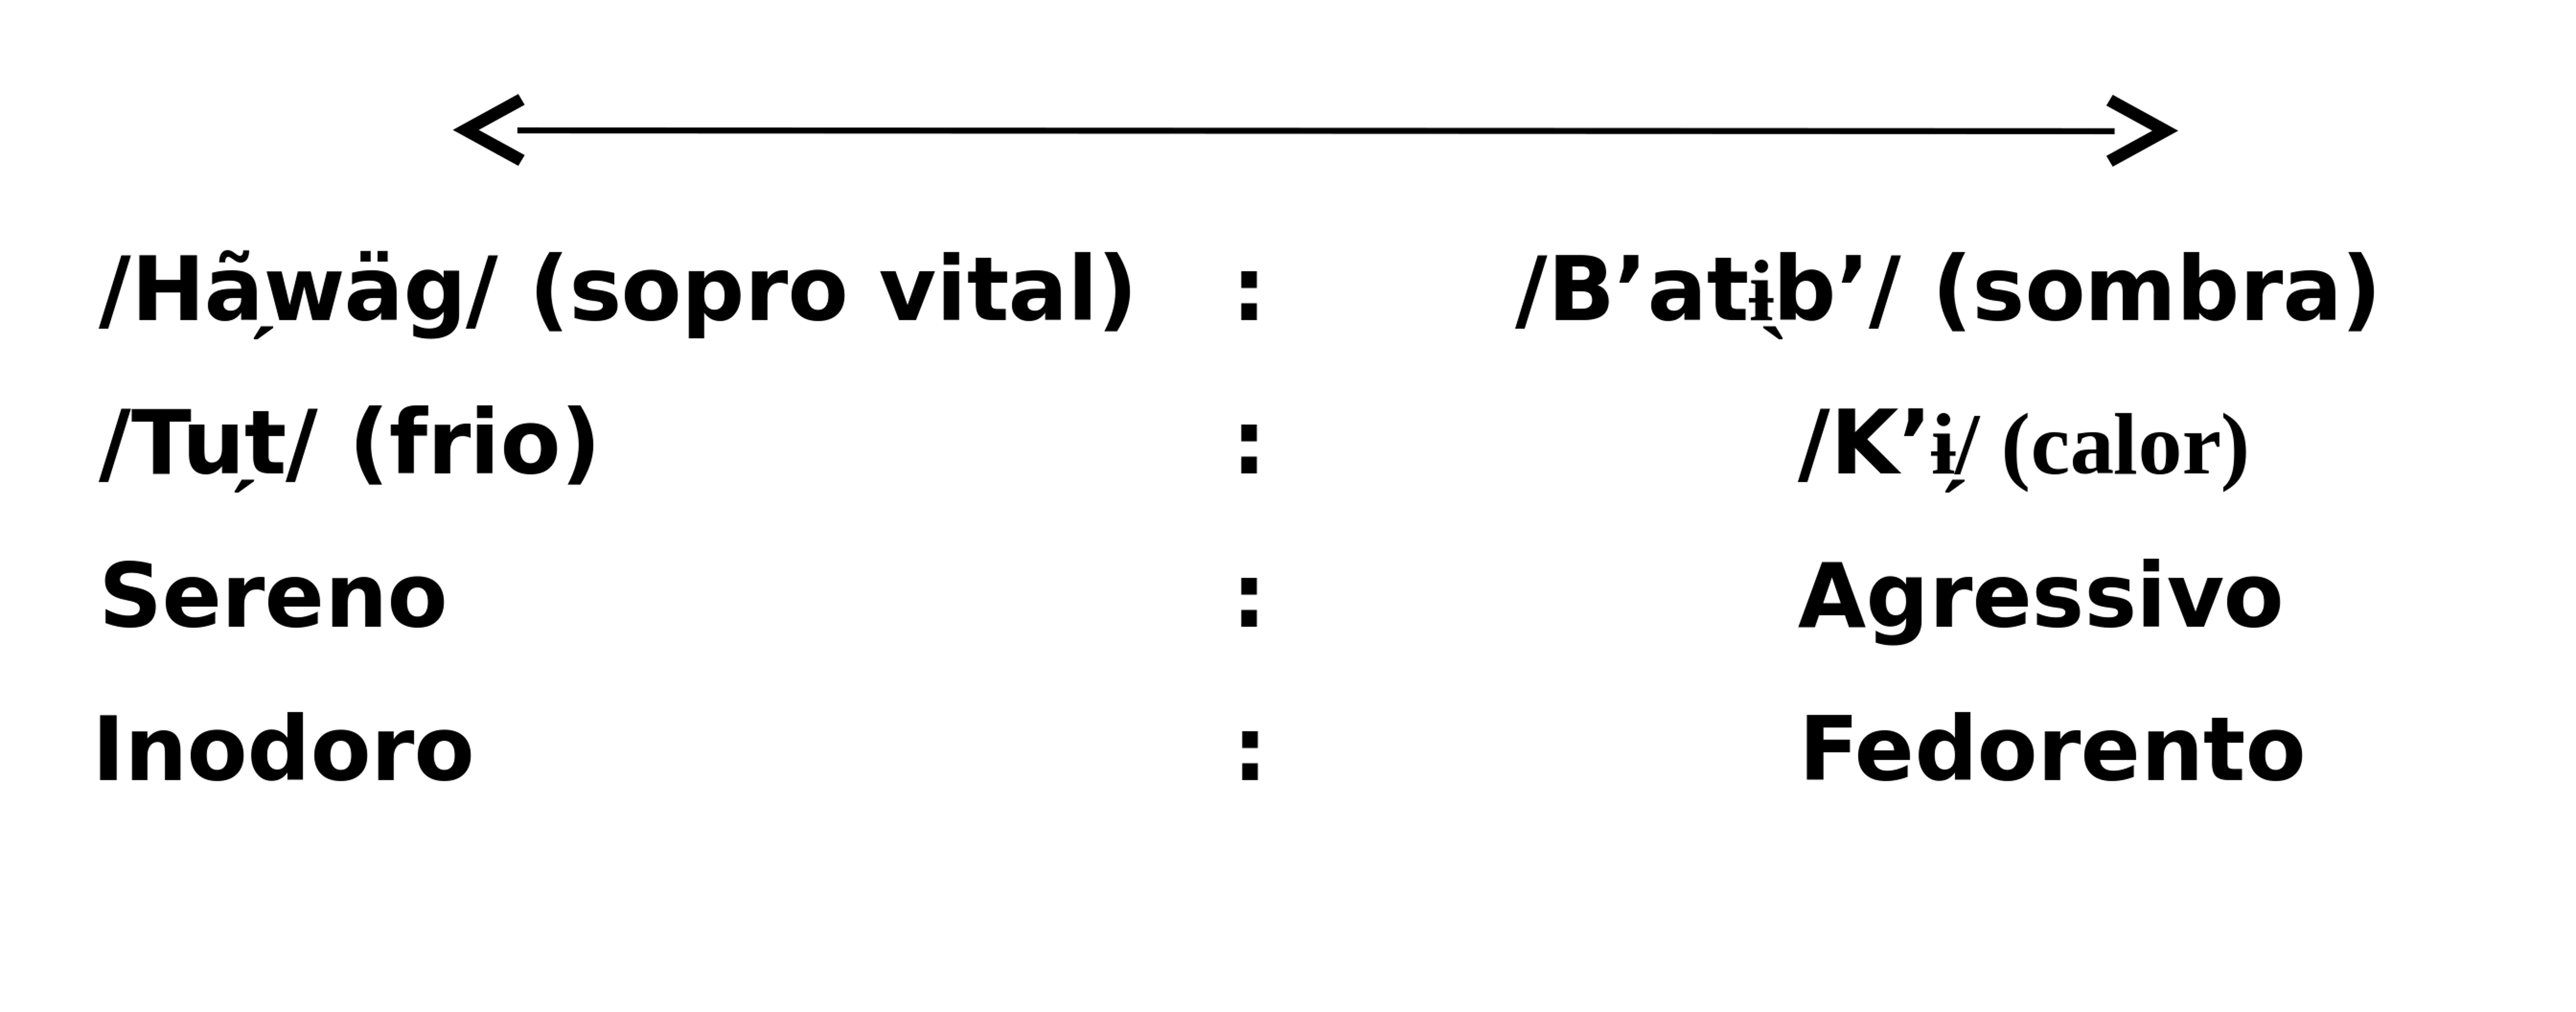
\includegraphics[width=\textwidth]{./img/q4_resize}
%\caption{Gradações de intensidade}
%\end{figure}

% Verificar tabela.
% \begin{center}
% \begin{table}[H]
% \centering
% \begin{tabular}{lcr}
% \leftarrow & \multicolumn{1}{l}{---} & \multicolumn{1}{l}{\hfill\rightarrow} \\
% \textit{Hã̗wäg} (sopro vital)    &                      & \textit{B'atɨ̖b'} (sombra)                            \\
% \textit{Tu̗t} (frio)             &                      & \textit{K'ɨ̗} (calor)                                 \\
% Sereno                    &                      & Agressivo                                      \\
% Inodoro                   &                      & Fedorento                                     
% \end{tabular}
% \caption{Gradações de intensidade.}
% \end{table}
% \end{center}


O recém"-nascido, \textit{molengo}, é um ser quente como sua mãe. Juntos
exalam odores intensos e têm grandes concentrações de sangue em seus
corpos, características que os tornam ofensivos seres malfazejos.
Analisando as restrições alimentares do sistema médico barasana e
taiwano, Langdon\footnote{1975, p.\,8.}) aponta que ``parece que tanto o sangue
menstrual quanto aquele que acompanha o parto são portadores de perigos
a toda a comunidade''. De forma semelhante, entre os Hupd'äh a presença
intensa de sangue faz com que seja perceptiva a evitação da casa nos
primeiros dias do pós"-parto. O casal permanece recluso com o bebê e
recebe apenas visitas do xamã e da senhora acompanhante. Esses perigos
que envolvem a presença excessiva do \textit{calor} nos corpos no pós"-parto
são bem contextualizados por Reid,

\begin{quote}
Para além dos limites das atividades culinárias, o sistema de energia
estende"-se também para a esfera ritual. Em períodos de crise, quando uma
pessoa está doente ou quando uma mulher dá a luz, aquele que está em
sofrimento deve apenas consumir comidas frias para conter as grandes
quantidades de Ku͂ Ponah que dominam o corpo. Quando executa benzimentos
de cura para pessoas doentes, o xamã deve alimentar"-se apenas de
alimentos \textit{frios} e evitar o contato com a luz do sol intensa ou com o
fogo. De modo inverso, um homem deve consumir alimentos \textit{quentes}
quando prepara o veneno de caça para fazer o veneno pegar. Aquele que
pretende praticar feitiços contra outra pessoa também come alimentos
quentes e evoca agentes \textit{quentes} para atacarem a vítima. Acredita"-se
que os Índios do Rio possuam mais Mair Ponah que os Hupdʉ, o que faz com
que tenham \textit{raiva} e perigosos feitiços. De modo semelhante, é a
presença de Ku͂ Ponah nos espíritos da floresta o que faz deles canibais
e malévolos.\footnote{1979, p.\,253.}
\end{quote}

Como os corpos dos seres humanos, todos os alimentos possuem equilíbrios
diferenciais de energias quentes ou frias. Após o nascimento, a mãe e o
pai devem, além de permanecer em resguardo na morada do casal, obedecer
às restrições alimentares. Durante os primeiros meses, a dieta baseia"-se
numa sequência progressiva de reintrodução de alimentos ao casal. O xamã
faz visitas constantes à casa para benzer cada um dos alimentos que vão
sendo oferecidos. Tendo um pedaço de beiju à mão, uma cuia com mingau,
um peixe ou pedaço de carne, o benzedor sopra o alimento mencionando
todas as plantas ou animais que pertencem à mesma categoria. Os óleos
são extraídos, as armas são repousadas e as cuias de \textit{caarpi} cercadas
para transformar o alimento em uma substância própria para o consumo. A
agência xamânica e a nutrição gradual levam ao resfriamento, à
desodorização e à pacificação dos corpos. Como mostra Århem para os
Makuna,

\begin{quote}
Benzendo os alimentos, os seres humanos transformam as pessoas"-animais
em alimentos humanos e, assim, afirmam sua humanidade. A capacidade
xamânica permite aos humanos superar os perigos inerentes à \textit{natureza}
e, ao mesmo tempo, incorporar a força vital que ela contém.\footnote{1996,
p.\,194.}
\end{quote}

O leite materno pode ser visto como um alimento composto essencialmente
por energia \textit{fria}, sendo comparável apenas a algumas frutas,
cultivadas e silvestres, e à água. A amamentação e a lactação
possibilitam, assim, o resfriamento dos corpos neonatais. Em
\textsc{b7}, o xamã menciona variedades de maniva e retira o óleo de
todos os derivados desse tubérculo para que a pouca quantidade de calor
desses alimentos seja neutralizada. O beiju, o mingau e a farinha passam
a ser a primeira fonte nutritiva do casal durante a \emph{couvade}.
\index{ah@\textsc{b}7\quad \textit{B'a' Bi'i̖d} \break Benzimento do Beiju}

Logo, frutas silvestres e da roça, como o \textit{si̖p}, ``biriba'', \textit{mi̖n},
``ingá'', \textit{dö̖g}, ``uirapixuna'', \textit{mo̗t}, ``tipo de cunuri'', \textit{pë̖d},
``cunuri'', \textit{sana̗}, ``abacaxi'', são reintroduzidas à dieta e, com o
tempo, começam a ser dadas ao bebê. São também muito consumidas durante
a gestação. O cubiu, fruta azeda, é uma das frutas prediletas das
gestantes por aliviar o enjoo. As formigas assadas, principalmente as
``manivaras'', \textit{kok'ã̗w}, são consideradas como um alimento não vegetal
rico em energia fria e, por isso, são boas para a refeição das
gestantes, sendo introduzidas já nas primeiras semanas da dieta
neonatal. Soma"-se a isso o fato de elas constituírem um alimento para a
\textit{troca de pele}, estando presentes na dieta da moça que passa pela
menarca e do rapaz que participa das cerimônias de \textit{Döhö d'äh},
Jurupari. Para endurecer a pele do bebê \textit{molengo}, as mulheres
alimentam"-se de frutas de árvores com casca dura de animais de couro
duro, como o jacaré, para que a criança seja \textit{tab'a̗'},
``dura'', ``resistente''.

\index{ah@\textsc{b}7\quad \textit{B'a' Bi'i̖d} \break Benzimento do Beiju}
Os vários tipos de pimenta mencionados em \textsc{b7} têm um papel muito
importante na culinária hup. Diferenciadas pelo grau de ardência, cor e
tamanho, as pimentas são o tempero necessário ao cozimento de peixes e
carnes pela sua propriedade de amainar o \textit{calor} e a agressividade
impregnados nesses alimentos. Para extrair a essência quente inerente à
própria pimenta, o xamã lava o óleo e cerca a cuia de \textit{caarpi} da lagarta
que come suas folhas. Como a gestação, a agência xamânica parece análoga
ao processo culinário, já que é um preparo para o consumo próprio das
substâncias. Pensando com Langdon, observa"-se que a sequência de menção
a tipos de alimentos em \textsc{b7} reflete uma ordem temporal de
reintrodução desses mesmos alimentos na dieta, cabendo à pimenta um
papel de transição entre vegetais e carnes.
\index{ah@\textsc{b}7\quad \textit{B'a' Bi'i̖d} \break Benzimento do Beiju}

Todos os seres designados como \textit{hu̗͂}, ``animais'', e como ``peixes'',
\textit{hõ̖p}, são fontes da essência \textit{quente} presente em maior grau no
sangue e na gordura, e em menor na carne, ossos e pele. Assim como os
humanos hup, também peixes e animais possuem \textit{hã̗wäg} e \textit{b'atɨ̖b'}. O
tamanho exacerbado desse segundo princípio vital faz com que a
característica fedorenta de seus corpos seja incorporada pelo
consumidor, que passa a exalar um forte cheiro. O abate da presa faz o
sopro vital e a sombra deixarem a carcaça, mas o calor, a agressividade
e o mau cheiro permanecem impregnados à carne e ao sangue. Esse odor
torna"-se perigoso por ser ofensivo aos \textit{parentes} das presas caçadas,
ofende igualmente seres como \textit{B'atɨ̖b'}, \textit{Bisi̗w}, Gentes"-Árvore, entre
outros. O tempo de cozimento em água ou de moqueio varia de acordo com o
grau de energia quente da carne, e seu consumo deve ser feito sempre com
pedaços de beiju, sumos de fruta e/\,ou manicuera. Nas palavras de Århem
(1996, p.\,194), ``comer envolve um processo de consubstanciação parcial
e identificação contextual entre quem come e a comida --- e, portanto,
também a potencialidade de o comedor ser `consumido' pela própria comida
que ele consome''. São os riscos representados por essa consubstanciação
entre o consumidor e o alimento que exigem a transformação xamânica e o
cozimento como pacificações simultâneas e combinadas dos pais, do bebê e
de seus respectivos alimentos.

Algumas grávidas dizem sentir náuseas com o cheiro e gosto de peixes
como o surubim, a \textit{b'ö̖y}, ``traíra'', o \textit{pö̗}, ``sarapó''. Isso as leva a
preferir o consumo de peixes mais \textit{frios}, como o \textit{poho̗t}, ``aracu'',
ou a piaba. As águas dos igarapés são tidas como mais frias que aquelas
dos rios grandes, o que parece delinear um critério de diferenciação
entre os peixes pelo calor de seus habitantes e também de seus corpos,
que variam de tamanho (grande ou pequeno), de forma (arredondado) e de
cor (prateada) em \textsc{b7}\index{ah@\textsc{b}7\quad \textit{B'a' Bi'i̖d} \break Benzimento do Beiju}. De acordo com uma gradação baseada nesses
princípios, os peixes vão sendo introduzidos à dieta do casal em
resguardo. O óleo é extraído e a agressividade é aplacada pelo
procedimento de cercar as \textit{tesouras}, armas laminares dos peixes e dos
\textit{piolhos}. Esses parasitas podem estar presentes nas brânquias do
peixe pescado sugando seu sangue.\footnote{Há uma atenção necessária às
  aberturas dos corpos de peixes e humanos hup devido aos perigos da
  entrada de substâncias e seres nocivos.} O consumo simbiótico de
parasita e hospedeiro, além de intensificar o calor, pode abrir sérias
feridas no corpo (leishmaniose).

Da copa das árvores para o solo, do chão ao subterrâneo, os \textit{hu̗͂},
``animais'', são progressivamente benzidos, tendo seus óleos lavados e
suas armas laminares cercadas. A atenção do xamã volta"-se, como no caso
dos peixes, para os minúsculos piolhos munidos de suas facas. Iniciando
pelo pequeno esquilo especificado por sua cor e por seu tamanho, fala"-se
para aves voadoras que possuem quantidade considerável de carne.
Cutiuaias e cotias, mamíferos que comem a fruta ucuuba, são os primeiros
animais de solo mencionados. A tendência dos \textit{pöhöy hũ̗ n'a̖n}, ``animais
do alto'', a serem herbívoros mostra"-se um critério importante porque
seus regimes alimentares permitem que tenham menos calor, cheiro e
agressividade em seus corpos. Animais carnívoros como as onças são
vistos como o extremo de concentração de essência \textit{quente}, pois
quanto maior o animal, maior será a quantidade de calor. A carne do
tamanduá, por exemplo, deve ser evitada durante a gestação e o resguardo
pelo odor intenso exalado pelo animal. O perigoso canto \textit{piha} de
oferecimento de \textit{caarpi} dos grandes mamíferos pode causar feridas no
corpo e fazer a pessoa sofrer com o \textit{choro enlouquecedor}.

Enquanto a ausência de carnes marca a dieta neonatal, durante a gestação
é importante que a futura mãe tenha uma alimentação carnívora, porque é
necessário aumentar a quantidade de sangue e calor em seu corpo para
formar e transformar o feto. As carnes de paca, cotia e macacos \textit{ö̗h} são
boas misturas, mas as carnes de ``tatu canastra'', \textit{o̖k}, e de
``tamanduá'', \textit{bɨ̗g}, devem ser evitadas. Não se pode comer animais que
tenham sido caçados com curare, pois o veneno, substância excessivamente
quente, pode fazer mal para o bebê e até mesmo causar abortos. Pode"-se
interromper uma gravidez indesejada consumindo"-se uma grande variedade
de plantas abortivas, os \textit{te͂h na̖m}, os ``curares de criança'',
conhecidas pelas mulheres desde a infância. Mantendo uma alimentação
carnívora equilibrada com muitas frutas, formigas e beiju, a gestante
assegura um aquecimento e o cozimento adequados ao desenvolvimento do
feto. Ao contrário, o superaquecimento leva a um cozimento que amolece,
apodrece o bebê, tendo como resultado o aborto. Como mostra
Lévi"-Strauss,

\begin{quote}
É patente o paralelismo com o cozimento por ebulição, cujos meios
culturais (recipientes) são preservados, mas o cozimento, este que é,
ele próprio, assimilado a um processo de autoaniquilação, uma vez que
seu resultado definitivo equivale, pelo menos verbalmente, a esta
putrefação que o cozimento deveria prevenir ou retardar.\footnote{1968, p.\,32.}
\end{quote}

Tão logo nasça a criança, o xamã sopra uma cuia de mingau mencionando as
panelas de plumas e pelos de aves e mamíferos, e vira o útero ao contrário
para impedir que o esperma entre no recipiente e molhe a argila. Essas
ações são fundamentais para que a mulher possa engordar, amamentar e
cuidar do recém"-nascido antes de conceber novamente.\footnote{Em termos
  ginecológicos, talvez esse encantamento aja invertendo a posição do
  colo e do corpo uterinos, bloqueando a continuidade entre o colo e o
  canal vaginal, algo que impede a passagem do sêmen (Bastos, 1971,
  p.\,5).} Quando o bebê começa a andar, esse 2º movimento do
encantamento, também designado \textit{benzimento do útero}, deve ser
desfeito para que o útero"-panela retorne à sua posição original e uma
nova gestação possa ocorrer. Se não for bem executado, o encantamento
pode impedir a boa lactação, esterilizar a mulher ou dificultar a
concepção. Uma nova gestação traz o perigo da concentração de sangue e
energia quente no corpo da mãe, impedindo o resfriamento, a
desodorização e o endurecimento do bebê. Como mostra Hugh"-Jones para os
Tukano,

\begin{quote}
No nascimento, na nominação, na puberdade e na iniciação, o kumu
controla as transições corporais e as transformações através da
manipulação de artefatos identificados com as partes do corpo.
Enunciados pelas divindades, os primeiros benzimentos afirmam essa
identidade, mas o processo se dá numa direção oposta --- longe dos corpos
concretos e próximo a artefatos mais abstratos que servem como sinais
para os componentes \textit{espirituais} desses corpos. Isso é o que permite
a socialização de pensamentos e de comportamentos~{[}\ldots{}{]}\footnote{2009,
p.\,47.}
\end{quote}

\index{ag@\textsc{b}6\quad \textit{Te͂h Bi'i̖d}\break Benzimento do filho}
A \emph{inversão da panela} pode ser vista como uma manipulação xamânica
desse artefato identificado ao útero que retoma a ação primordial de
junção do \textit{hãwäg} da mãe às margens do Lago de Leite (\textsc{b6}). As
panelas de plumas e os bancos de plumas são artefatos, potências
primordiais cujo manejo assegura a concentração da pessoa, o aleitamento
e o resfriamento dos corpos. Ao banhar o corpo da mulher ritualmente com
a fumaça da folha \textit{bu̗y k'e̖t}, o xamã faz com que ela se sente nos bancos
de plumas de patos e pássaros. Do mesmo modo como as plumas aumentam o
volume corporal das aves, elas engordam a mulher para que esta tenha
bastante leite e nutra seu bebê. Engordar a mãe e o recém"-nascido são
objetivos comuns que se tornam possíveis pelo resguardo, pela dieta
gradativa, pela interdição do intercurso sexual e pela ação xamânica.

``Quando chove, a água cai nas penas dos pássaros e vai embora, não
molha. Também a libélula joga a água para cima, espalha\ldots{}'', foi
como Samuel me explicou por que o benzedor menciona o curiango e a
libélula em \textsc{b7}\index{ah@\textsc{b}7\quad \textit{B'a' Bi'i̖d} \break Benzimento do Beiju}. Os insetos voadores devem ser desarmados, mas é
graças à semelhança criada entre as mães e as libélulas que o esperma,
uma água, é jogado longe, espalha"-se e não \textit{molha} o útero. As
panelas"-de"-plumas do jacuaçu, do urumutum, do mutum e as
panelas"-de"-pelos de mamíferos (como a preguiça, o tamanduaí, o guariba)
têm em comum com as asas dos insetos a propriedade de espalhar a água da
chuva. A não aderência da água, uma impermeabilidade, dispersa o
esperma, a água, evitando que a \textit{chuva fecundante} leve à nova concepção e
coloque em risco o desenvolvimento do bebê.

Para conseguir fechar o útero, o benzedor gira as panelas de plumas ao
contrário. Com isso, ele inverte a posição da abertura uterina, voltando
a boca da panela para o cóccix e o fundo para o canal vaginal. O ferrão
da caba ajuda a extrair o pedaço duro de casca de turi com o qual o xamã
vedará definitivamente a abertura vaginal. As mulheres assemelham"-se às
cabas, tornam"-se cercadas, tapadas em baixo, e não engravidam. Se em
\textsc{m16}\index{25@\textsc{m}16\quad A gestante tapada}, o pai abre a mãe para o nascimento dos gêmeos, abrindo uma
mulher tapada, em \textsc{b7}, o xamã tapa as mulheres abertas para
protegê"-las dos riscos de uma nova fecundação. Essa rotação que veda
assemelha"-se, em maior escala, à criação da barreira intransponível que
cerca o \textit{útero ctônico} da Casa"-dos"-Animais para impedir a saída de
presas e a entrada dos xamãs hup.\footnote{A temática da mulher tapada
  foi amplamente analisada por Lévi"-Strauss surgindo ora como uma esposa
  incompleta por impossibilitar a cópula, ora como uma grávida que
  precisa ser aberta, perfurada para que seja esvaziada das crianças que
  contém (2004b, p.\,221).}

\index{ah@\textsc{b}7\quad \textit{B'a' Bi'i̖d} \break Benzimento do Beiju}
O que está em jogo em \textsc{b7} é o ganho de peso da mulher articulado
ao resfriamento e à desodorização dos corpos consubstanciados para
assegurar a nutrição apropriada do bebê. O corpo da mãe é um instrumento
que, ao transformar as substâncias, constrói o corpo da criança.
Enquanto a gestação pode ser vista como um processo de cozimento uterino
que gera e desenvolve o feto, o aleitamento parece ser um processo de
resfriamento que, a partir da dieta materna benzida, garante a
desodorização e a atenuação do sangue que tanto ofendem os seres
malfazejos e coloca em risco toda a comunidade. O manejo da
panela"-útero, um artefato corporal, mostra"-se um movimento tenso de
manipulação de potências primordiais porque, embora assegure o
crescimento do bebê, pode causar esterilidade à mãe. Graças à ação
xamânica e aos esforços de \textit{busca do filho}, Tereza e Elias
conseguiram conceber novamente. Em 2012, partilhei a felicidade da
chegada da recém"-nascida à aldeia e o empenho coletivo dos \textit{comedores
de coca} para curar e proteger a bebê através da dieta de reintrodução
progressiva dos alimentos benzidos.

\section{A mãe sentada}\label{a-muxe3e-sentada}

O local do parto deve ser preparado previamente pelo xamã. Com a fumaça
do breu, ele defuma para cercar a casa, a roça ou a área próxima a um
caminho, espaço previamente escolhido pela mulher para ter o bebê.
Nenhum homem pode aproximar"-se do local depois que ele estiver
preparado. \textit{Te͂h su̗' hipã̗h nɨ̗h}, ``a mulher não saberá parir'' se houver
a presença masculina na hora do parto. O mesmo perigo corre a mulher que
vê as flautas Jurupari ou que passa a comer coca com os senhores. Assim,
da mesma forma como é interditado às mulheres ver as flautas Jurupari, é
vedado que os homens vejam o nascimento. Mesmo o xamã deve afastar"-se e
reencontrar a mãe apenas depois que ela já estiver com o bebê. Sempre
protegida do sol, devido à ameaça de \textit{Wero̗ Hup Te͂h i͂h}, a mulher
acocora"-se.

É geralmente uma senhora quem acompanha o parto. Seu vínculo com a mãe
pode ser de consanguinidade, mãe ou tia (\textsc{m}, \textsc{mm}, \textsc{mz}), ou de afinidade
(\textsc{hm}, \textsc{hd}) dependendo da configuração do casamento como bilocal ou
virilocal. Essa \textit{bab ni ãy}, ``acompanhante'', é considerada uma pessoa
experiente por ter se sentado muitas vezes sobre seu próprio banco de
leite para dar à luz. Além disso, a presença da anciã é também a
participação de uma senhora que não menstrua mais, algo importante, já
que o sangue feminino é tido como perigoso. É comum que a acompanhante
do parto cuide da gestante durante toda a gravidez, alimentando"-a e
curando"-a.

A velha senhora cuida da alimentação da gestante e do casal nas
primeiras semanas, quando a mãe não pode tocar os utensílios de cozinha.
Os \textit{s'u̖g yõh}, ``remédios do mato'', são trazidos da roça ou dos
caminhos pela acompanhante, caso a gestante sinta dores ou tenha algum
tipo de sangramento. Quando necessário, a acompanhante solicita que um
xamã benza o remédio a ser oferecido à gestante. Aquela que já se sentou
muitas vezes em seu banco é, igualmente, uma mulher seca ou fechada, por
não conceber mais. Não estará menstruada no momento do parto e poderá,
portanto, orientar e cuidar bem da mãe e do bebê.

Como já foi visto, os bancos em que os benzedores se sentam para
conversar e benzer são igualmente denominados \textit{bancos de leite} ou
\textit{bancos da vida}. Ainda que não esteja sentado em um banco de sorva, a
postura acocorada ou sentada no chão com o tronco curvado para frente e
as pernas contraídas é igualmente denominada \textit{banco da vida}. Sentado
sobre seu banco, o xamã sopra o cigarro. Enquanto a acompanhante cuida
do preparo dos alimentos, o xamã benze cada tipo de alimento que vai
sendo reintroduzido ao casal. Caso a mãe não tenha leite para alimentar
o bebê, um benzimento é realizado para que seus seios \textit{pud"-dë̖h bë̗y},
``mostrem o leite''. Ao longo de sua jornada, o xamã \textit{dá banco} aos
machos dos diversos seres que podem fazer mal, seja pelo calor (febre e
dores de cabeça), pelo \textit{caarpi} (choro enlouquecedor), pela intolerância
ao odor humano (abdução do \textit{hã̗wäg}) ou pelas armas laminares (feridas).
Como a \textit{parteira}, o benzedor faz a mãe sentar"-se no banco de leite
(cócoras).

Desse modo, as ações do xamã, um velho que se senta todas as noites em
seu banco de leite para proteger e regenerar a vida, e as da
acompanhante, uma senhora que já se sentou muitas vezes em seu banco de
leite para dar à luz, parecem ser complementares e fundamentais para o
nascimento. Como o sangue menstrual, o sêmen masculino também atrai e
causa a fúria dos seres malfazejos pelo seu odor. Por isso, o velho
benzedor, um \textit{comedor de coca}, e um \textit{tɨ̗b we̖y meh}, ``pênis mole'', e
a senhora que passou pela menopausa tornam"-se pessoas adequadas para
auxiliar o processo de nascimento. As ações \textit{hã̗wägät} do xamã agem
durante o acontecimento do parto. Manifestam sua presença sob outro
regime corporal, já que a participação masculina representa perigo. De
modo diferente, a acompanhante age \textit{sa̗pa̗t}, como pessoa corporificada
estando sempre ao lado da parturiente.

\index{ag@\textsc{b}6\quad \textit{Te͂h Bi'i̖d}\break Benzimento do filho}
Em \textsc{b6}, o xamã deve fazer sentar a mãe sobre seu banco de leite
e, ao mesmo tempo, tirar o banco primordial da criança para que ela
deixe o útero. Como me contou Catarina, com o auxílio da acompanhante, a
gestante se posta de cócoras. Para manter o equilíbrio em meio às
contrações e à força para os esforços expulsivos, a mãe ampara"-se na
rede, caso esteja em casa, ou em um galho de árvore, se estiver na roça.
Ajudada, a mãe abre bem suas pernas, alarga ao máximo a abertura vaginal
para que, a partir da coxa (fêmur e paleta) e da cintura pélvica (ilíaco, osso do quadril), concentre suas forças para empurrar o bebê.
Assumindo essa postura, a mulher senta"-se em seu banco de leite, um
alinhamento corporal formado pela contração da coxa e da cintura
pélvica, assume a postura primordial para trazer uma nova pessoa à vida.
O xamã sentado e a mãe acocorada tiram o banco da criança para que ela
se desloque do Lago de Leite à aldeia, do ventre aos braços da mãe.

A obstetrícia designa como posição vertical a postura acocorada assumida
por gestantes para dar à luz, diferenciando"-a da postura do decúbito
dorsal ou supina, com a pessoa deitada horizontalmente de barriga para
cima, posição normalmente adotada pela biomedicina para a realização dos
partos. Estudos atuais apontam que a posição vertical não diminui o
fluxo sanguíneo, como acontece na posição dorsal, reduz a duração do
período expulsivo, diminui a dor e possibilita a menor alteração nos
padrões de batimentos cardio"-fetais. Postando"-se em seu banco de leite
com a ajuda da acompanhante, a parturiente alinha"-se corporalmente,
encontra sustentação no fêmur (coxa) e no quadril (cintura pélvica) para
o movimento expulsivo, alivia a dor e sustenta"-se como as fêmeas para
parir.

\index{25@\textsc{m}16\quad A gestante tapada}
Ainda que não sejam mulheres tapadas (sem ânus nem vagina)
(\textsc{m16}), as mães hup têm pequenos orifícios se comparadas às
fêmeas mamíferas. Postar"-se sentada no banco de leite é uma habilidade
comum à mulher hup e às fêmeas que também contraem a região do fêmur e
do quadril para dar à luz. A sequência de interações xamânicas com as
fêmeas animais estabelece"-se como uma gradação que parte dos seres de
menor tamanho para, apenas no final, fazer menção à grande égua. A
homologia entre os bancos de leite expande gradativamente a estrutura
corporal materna. O xamã parte da paca, um roedor de médio porte (de 61--77\,cm, e 5--13\,kg), passa pelo caititu (de 70--90\,cm, e 17--30\,kg), pelas porcas (de 95--1.10\,m, e de 25--40\,kg), pelas antas (de
1.70--2,10\,m, e 227--250\,kg) e, por fim, menciona a égua, um grande
mamífero (de 1.50--1.60\,m, e 450--550\,kg). No sentido inverso,
fala"-se para os filhos dos mamíferos pequenos, fazendo com que o bebê
reduza sua dimensão corporal e passe mais facilmente pela abertura
vaginal alargada.

\textit{Roedora} é uma das formas dos homens hup referirem"-se às vaginas,
quando conversam sobre a vida sexual. Assim, ao mencionar a paca, o xamã
aproxima"-se dessa percepção anatômica do órgão sexual feminino como uma
boca pequena que rói o pênis. De acordo com Bonatelli, uma das
características notáveis da paca quanto a seu sistema reprodutivo vem a
ser o fato de seus membros pélvicos serem muito musculosos. Os animais
adultos apresentam dimorfismo sexual, o que permite diferenciar machos e
fêmeas pelo tamanho e formato da cabeça. Nos machos a cabeça é mais
achatada e larga, enquanto nas fêmeas a cabeça é mais fina e esguia. O
primeiro cio pode ocorrer com aproximadamente um ano de idade, período
em que os machos também iniciam a atividade sexual. O período de prenhez
é em média de 115 dias, nascendo um filhote na maioria dos casos, e,
raramente, dois ou três. As pacas vivem em casais monogâmicos num dado
território, mas deslocam"-se sempre separadamente à procura de alimentos
(frutas, brotos, raízes e tubérculos). Têm hábitos noturnos e podem ser
encontradas nas margens de grandes rios. Durante o dia mantêm"-se em
tocas (troncos ocos, buracos) com os orifícios vedados por folhas.

Os caititus e os porcos possuem sistemas reprodutivos semelhantes aos
dos suínos domésticos, acasalam"-se em todas as épocas do ano e possuem
placenta. As gestações são de 144 a 148 dias para os catetos e de 156 a
162 para os porcos"-queixada. A cada gestação são gerados dois filhotes,
em média, podendo, às vezes, nascer um ou três. Os caititus e os porcos
são animais gregários de hábitos diurnos, deslocam"-se em manadas de até
20 indivíduos (caititus) e de 50 a 300 indivíduos (porcos) por trilhas.
Ambos têm fortes odores que se acentuam quando são surpreendidos. Dormem
em buracos na terra e sob as raízes das árvores. Alimentam"-se de frutas,
castanhas e brotos, mas os porcos comem também lesmas e pequenos
animais.

Entre os mamíferos das terras baixas, as antas e os cavalos pertencem à
mesma ordem, \emph{Perissodactyla} (\emph{equidae},
\emph{rhinocerotidae}, \emph{tapirus}). Segundo May Jr., o ciclo
reprodutivo da anta é lento. A maturidade sexual ocorre por volta dos
quatro anos de idade. A gestação, que dura de 395 a 399 dias, gera um
único filhote e o intervalo entre gestações é de 18 meses, algo que
causa rápidos declínios populacionais quando uma população é alvo
constante da caça. No que diz respeito à reprodução equina, a idade
média de puberdade das éguas é de 12 a 15 meses. Um único filhote é
concebido por gestação. O olfato é fundamental para a reprodução dos
equinos, pois o macho sente"-se atraído pelos odores exalados pelos
genitais externos da égua, aproxima"-se, exibe"-se e inicia tentativas de
monta (cópula). O período médio de gestação oscila entre 335 e 340 dias,
havendo maior duração na gestação de fetos machos que na de fêmeas (dois a
sete dias a mais). Próximo ao momento do parto, as éguas afastam"-se para
dar à luz solitariamente. Começam a caminhar nervosas em círculos quando
a bolsa se rompe, e iniciam movimentos de tombar e levantar repetidas
vezes. Segundo Evans, quando o potro está saindo, as extremidades
anteriores e o tronco passam com facilidade, mas no momento em que a
bacia do feto penetra a pélvis da égua, \textit{pode produzir"-se um ligeiro
descanso}. Suponho que seja esse \textit{descanso}, uma postura sentada a
que \textsc{b6} faz referência, seja o ato de sentar"-se sobre o banco de
leite comum às fêmeas e às mulheres hup.
\index{ag@\textsc{b}6\quad \textit{Te͂h Bi'i̖d}\break Benzimento do filho}

Na sequência: paca \textgreater{} caititu \textgreater{} porco
\textgreater{} anta \textgreater{} égua, além da gradação crescente
das aberturas femininas, o tempo da gestação aumenta à medida que se
passa de um mamífero ao outro. A quantidade de filhotes por gestação,
que varia de um a três nos menores, passa a ser de um único filhote nas
antas e nas éguas. Amplia"-se também o intervalo entre as gestações e
restringe"-se a variabilidade do regime alimentar que, nos equinos, tem
como base as gramíneas. Se a paca evoca o ato sexual, a vagina roedora,
a égua parece relacionar"-se à dieta alimentar baseada exclusivamente em
beiju e mingau, ambos de origem vegetal (maniva). O forte odor, traço
marcante dos catetos e porcos, atenua"-se na anta e na égua, sendo que a
anta toma banhos frequentes de lama e água para aliviar"-se dos
carrapatos e moscas. Considerando"-se que a restrição alimentar e os
banhos diminuem os odores exalados pelos corpos da mãe e da criança, a
identificação passa de fedorentos a desodorizados. O aumento do
intervalo entre as gestações, igualmente gradativo nessa sequência de
fêmeas, é visto como importante para que as mulheres hup possam nutrir e
cuidar bem do bebê e, ao mesmo tempo, consigam recuperar"-se da gravidez
e engordar. O padrão de gestação de um único filhote no caso das antas e
éguas reflete o ideal de não gemelaridade gestacional hup, já que o
segundo rebento é considerado um \textit{b'atɨ̖b}, fruto do intercurso sexual
involuntário da mãe com um ser malfazejo. Um último aspecto comum às
fêmeas mencionadas em \textsc{b6} vem a ser sua mobilidade, que, como no
caso da paca, contribui para que todas tenham membros pélvicos
musculosos, como observa Descola,
\index{ag@\textsc{b}6\quad \textit{Te͂h Bi'i̖d}\break Benzimento do filho}

\begin{quote}
Essas restrições geram dois tipos de consequências para as populações de
herbívoros terrestres (pacas, antas, roedores e veados): de um lado, uma
frágil densidade geral engendrada pela dispersão do material vegetal
comestível e, por outro lado, uma tendência à mobilidade, principalmente
para as espécies gregárias que precisam forragear por vastas áreas de
nomadismo.\footnote{1986, p.\,77.}
\end{quote}

A vida gregária e a mobilidade para a procura de frutos e grãos
dispersos em vastas regiões são aspectos relevantes para a fabricação da
corporalidade da parturiente. Como visto, o feto desenvolve"-se em meio
aos afazeres diários da mãe, que se desloca continuamente para a roça e
vota com seu cesto carregado para fortalecer seu banco de leite. A ação
cotidiana de intervenção sobre o corpo e a semelhança com os animais
nômades potencializam a estrutura pélvica da mãe e criam essa intenção
para a sociabilidade, algo que talvez remeta ao excessivo exercício de
respeito às interdições para que, através de seu comportamento, a mãe
deixe de expor a comunidade aos perigos que sua condição representa. Há,
assim, um engajamento prático da mãe com a materialidade de seu próprio
corpo para gerar a forma banco de leite para dar à luz. A ação xamânica
complementa esse esforço cotidiano inserindo a mãe num campo relacional
orientado pela habilidade dos deslocamentos e do parto.

Portanto, fazer sentar revela"-se uma ação fundamental para que a mulher
hup adquira progressivamente os atributos corporais e sociais da
maternidade como uma habilidade. A agência xamânica promove a interação
da gestante com as fêmeas a partir de uma sequência específica que
transforma e protege à medida que se passa da pequena roedora à grande
ruminante. O banco de leite coloca"-se como uma postura anatômica e
relacional favorável à imitação e à metamorfose corporal que tem na
observação do comportamento e da morfologia de certos animais um
horizonte importante de referência generativa.

\index{af@\textsc{b}5\quad \textit{Ti̖wi̖t hamap bi'i̖d ta'}\break Benzimento dos caminhos}
Em \textsc{b5}, para proteger os viajantes das ameaças do percurso, o
xamã dirige"-se para dentro do corpo do esquilo marrom, para dentro do
corpo da onça pequena. Mamíferos, esses animais ocultam os andarilhos
com seus corpos e pedaços de tabaco. Um processo de contração, redução
corporal, invisibiliza e protege. Num sentido inverso, vestida de \textit{Döh
Ã̗y}, a mulher hup revela"-se uma insaciável amante, dona de uma enorme
vagina, e uma devoradora de homens, dona de uma boca ferina
(\textsc{m4}). O vestido de Branca maximiza sua corporalidade e sua
ferocidade, fazendo os homens correrem para não vê"-la. Ou seja, o
processo de expansão corporal de \textit{Döh Ã̗y} acentua sua visibilidade,
indesejada pelos viajantes.\index{13@\textsc{m}4\quad A \textit{Dö̗h Ã̗y} e seu marido}

Desse modo, talvez a pequena paca ajude a ocultar a mãe quando sua
abertura ainda é reduzida, e uma visibilidade cada vez mais acentuada vá
fazendo a mãe ser temida pelo tamanho, pela força e pelo grito. Nesse
sentido, creio que a égua, um animal de branco, aja como o vestido de
\textit{Döh Ãy} nesse momento de extremo aquecimento e sanguinidade corporal. A
égua possibilita que a mulher hup tenha uma vagina gigante, uma força
exacerbada, uma grande rapidez, tornando"-se perceptível e temida.
Enquanto a \emph{mulher} \emph{sedutora canibal} potencializa a
sexualidade, a predação e o apetite canibal de uma caçadora feroz, a
\emph{fêmea} \emph{ruminante sentada} intensifica a maternidade, o tônus
pélvico, o vegetarianismo, a intenção para a sociabilidade e para o
respeito às interdições necessárias à segurança durante o parto e o
resguardo. A identificação físico"-gestual à égua age, assim, como a
roupa de muçurana que veste os andarilhos e apavora as jararacas.

Além de transformar a postura corporal feminina, fazendo sentar e
abrir"-se, o xamã e a acompanhante devem intervir para transformar a
gestualidade sonora materna. O gemido de dor, perigoso para os ouvidos
das crianças, precisa tornar"-se um grito de ordem (gemido"-grito).
Enquanto o gemido pode ser considerado como um som contínuo de
lamentação que varia de acordo com a intensidade da dor ou estímulo, o
grito configura"-se como um som forte emitido de forma direta, intensa e
descontínua. Como gemido, o gesto vocal aproxima"-se, por um lado, ao som
das mulheres durante o intercurso sexual e, por outro, à lamentação em
decorrência da dor. Como o barulho do Trovão, o gemido da mãe suja a
\textit{b'oto̗k"-moy}, a Casa"-da"-Audição, ou o ``ouvido'', e faz com que a criança
sofra com o \textit{choro enlouquecedor}. Os contínuos urros de desconsolo do
bebê sujam o ouvido dos xamãs, impedem que pensem, conversem e benzam
corretamente. Desse modo, o barulho do \textit{choro enlouquecedor}, um
lamento emitido pela criança, torna as famílias vulneráveis aos ataques
dos seres malfazejos. Como os benzedores não conseguem cercar as
pessoas, o choro faz com que todos estejam visíveis e
desprotegidos.\footnote{Segundo Lévi"-Strauss, a equivalência entre gritos
  e sujeira faz com que esses termos sejam mutuamente conversíveis
  ``conforme o mito escolha um código acústico, alimentar ou sexual para
  se exprimir'' (2004b, p.\,360).}

\index{ag@\textsc{b}6\quad \textit{Te͂h Bi'i̖d}\break Benzimento do filho}
Com o grito de ordem, a voz materna metamorfoseia"-se em voz de mãe"-paca,
de mãe"-porca, de mãe"-égua que não sentem dor e ordenam ativamente a
saída de seus filhotes.\footnote{Seria interessante comparar as fêmeas
  mencionadas em \textsc{b6} à sarigueia nutriz, tal como surge no mito tupi
  analisado por Lévi"-Strauss (2004b), pois essa fêmea limpa as secreções
  fétidas de suas tetas e não sente dor ao parir (2004b, p.\,269).} Do
lamento (gemido), uma atitude paciente e passiva, a parturiente torna"-se
agente a partir de sua própria iniciativa (grito). Os caititus e os
porcos são animais quietos, mas emitem um \textit{latido} quando
surpreendidos. Já as antas são consideradas silenciosas, pois se
comunicam por assobios, mas bufam caso se sintam ameaçadas. As éguas
relincham sonoramente e defendem"-se empinando o corpo e investindo suas
patas traseiras ou dianteiras em coices contra a pessoa ou animal que
lhes cause insegurança. Seus sons são percebidos como gritos que ordenam
a saída, o afastamento. Analogamente, durante o parto, esses sons
protegem a fêmea da dor e suscitam uma expulsão precisa do feto.
Gritando, a mãe hup concentra sua potência sonora numa emissão intensa
e, ao ordenar a saída do bebê corretamente, cerca, protege o ouvido e o
pensamento da criança dos gemidos contínuos que sujam e causam
sofrimento a todos.

Dentro da Casa"-dos"-Animais, o eco do tambor de pedra fazia com que os
xamãs libertassem os animais para a floresta. \textit{Tããw} era o som forte e
preciso que Ponciano fazia com a boca para imitar o poderoso eco que
percorria as paredes rochosas, fazendo com que, \textit{Bisi̗w}, um terrível
dono dos animais, cedesse presas aos caçadores. O interior de sua morada
é visto como uma grande aldeia plena de festas, Dabucuris dos animais
que não param de copular e reproduzir"-se. Como mencionado, do alto de
\textit{Hu͂ya̗w"-Paç}, o grito assustador de \textit{Dö̗h Ã̗y} afugenta os caçadores que
passam da posição de predadores à de presas medrosas. O grito de ordem e
a percussão ritual podem ser vistos, nesse sentido, como gestos
imperativos de mando que provocam a saída ou a fuga das presas. Se o
grito das fêmeas expulsa os filhotes do útero, o eco do tambor rochoso é
também uma emissão sonora precisa que ordena ao dono dos animais a saída
das presas. Grito materno e estrondo rochoso abrem a mãe (útero) e o
morro (útero ctônico). A saída dos animais para a floresta mostra"-se uma
ação análoga ao parto, já que o movimento de expulsão imperativa e
precisa é suscitado pelo som potente da percussão da rocha e da voz.

\textit{Ye̗͂h}, ``mandar'', ``ordenar'', vem a ser uma atitude fundamental na relação
dos pais com seus filhos. Apesar do respeito que há à vontade das
crianças, saber mandar é importante para que todos participem das
atividades da casa e não queiram apenas \textit{ya̗ga̗t ni̗i̗}, ``estar na rede''.
Logo cedo, a mãe ordena que as filhas tragam água, enquanto um filho
mais velho já está cortando a lenha para fazer fogo. Meninas e moças
saem com a mãe para a roça e voltam com seus pequenos aturás plenos de
frutas e manivas. Os meninos saem para pescar com o pai e, logo, trazem
pequenos peixes. A ajuda alterna"-se com as brincadeiras e com as
atividades escolares, mas o pedido dos pais deve ser respeitado como uma
ordem.

Desse modo, quando a mãe reverte seu gemido em grito e ordena a saída da
criança, ela inicia um processo educativo, fazendo com que a criança não
queira \textit{ficar apenas em sua casa}. O bebê sentado que sovina suas
coisas tem uma atitude antissocial. Recusa"-se a deixar sua morada
uterina, recusa"-se a obedecer e recusa"-se a dar seus pertences.
Obedecendo à ordem, o bebê entrega seus pertences ao xamã como uma
dádiva. Ao mesmo tempo, cedendo suas armas, ele atende a um chamado
sedutor e lança"-se como uma presa frágil aos braços de sua mãe. Deixa o
útero como um filhote de paca, de porco, de anta, de égua, saindo, ao
fim de seu ritual de crescimento, pela grande abertura. Pensando com
McCallum, com o grito de ordem a mãe inicia a socialização da criança a
partir de uma \textit{pedagogia prática} que a faz, através de seu próprio
gesto de dar seus pertences, aprender princípios de reciprocidade e de
hierarquia que orientam as relações sociais. A expulsão do útero
introduz o bebê num contexto propício para perceber e agir em
consonância com esses preceitos aprendidos no curso de sua ação.

Na interpretação de Hugh"-Jones (2009, p.\,47), ``Como os benzimentos
deixam claro, estes artefatos são os resultados e índices de seus
pensamentos e intenções, e signos dos corpos humanos que futuramente
criarão, uma criação que se desloca do pensamento, por meio do artefato,
em direção ao corpo''. Seguindo Hugh"-Jones, é possível dizer que o banco
de leite relaciona"-se a uma estrutura óssea comum a animais e humanos
que permite assumir a postura ritual adequada para a ação xamânica e
para o nascimento. As fêmeas mamíferas servem de referência para o
alinhamento da atenção da mãe, que, dotada de uma corporalidade
expandida, consegue orientar seus movimentos para trazer seu filho ao
mundo a partir de seu banco de leite e de sua voz. A mãe insere"-se num
campo de força através de seu engajamento ativo e sensorial com a
materialidade de seu próprio corpo, o qual tem, na postura e musculatura
das fêmeas, horizontes de habilidade a seguir. Concentrando e
potencializando suas forças, as parturientes tornam"-se hipermulheres
sentadas sobre bancos e corpos animalizados. Abrem suas vaginas
expandidas e gritam para ordenar a saída do filho. O banco de leite, que
permite aos xamãs a postura adequada para comer coca, conversar e
benzer, possibilita que a mãe tenha forças para deslocar o filho do
útero para o mundo.

%\section{Filhotes e filhos}\label{filhotes-e-filhos}

\section{A mãe tamanduá e seu
filhote}\label{a-muxe3e-tamanduuxe1-e-seu-filhote}

\textit{Bɨ̗g ã̗h me̗h yɨ̗'ɨ̗h. Ayu̖p ã̗y pö̗g. Tɨnɨ̖h te͂h pɨ̗d}, ``Matei um tamanduá, uma
mãe com seu filhote'', comemorou Samuel logo que chegou da roça. À
tarde, enquanto caminhava com seu cachorro Juto, ouviu o som das
folhagens chacoalhando. Latindo, o cão avançou por entre as árvores.
Corria de um lado para o outro rosnando sem parar. Aproximando"-se,
Samuel viu uma enorme tamanduá"-bandeira acuada, tentando proteger seu
filhote das investidas do canino. Quando sentiu a presença do caçador,
ela disparou correndo. Samuel perseguiu o bicho empunhando seu terçado.
Com um golpe, feriu o rabo do animal que diminuiu a velocidade. Com duas
terçadadas, atingiu a fêmea na cabeça e no longo focinho, que logo em
seguida estatelou"-se no chão. Depois disso, foi fácil matar o filhote
que tentava, inutilmente, escapar do cachorro. Novamente, um golpe de
terçado tirou a vida do pequeno tamanduá. Samuel cobriu a mãe com
folhas, mergulhou a carcaça do filhote na água para escondê"-lo e
retornou para pedir ajuda a seu irmão Sabino, a sua esposa Virgínia e a
mim.

Naquele final de tarde, os caçadores, acompanhados de suas respectivas
esposas, voltaram para recolher as presas. As mulheres carregaram seus
aturás, que logo ficaram repletos com os membros esquartejados das
vítimas. O bucho dos animais foi descartado, mas os órgãos internos
somaram"-se à incrível quantidade de carne obtida. Primeiro, as presas
foram incineradas para a queima dos pelos e do couro. Em seguida, Samuel
cuidou do corte da carne, dividindo as partes que seriam de consumo
próprio, as que seriam dadas a seu irmão e, uma terceira, ao seu pai.
Afinal, Ponciano teria que benzer a carne para que não causasse feridas
ou \textit{choro enlouquecedor} às crianças.

Enquanto cortava a carcaça, Samuel explicava"-me sobre a anatomia do
tamanduá. O rabo é o ``remo'', \textit{he̖͂y' b'ah}, que faz com que o animal
corra rapidamente em sua fuga. Suas garras perigosas são suas \textit{yö̗k
b'ah}, ``espadas primordiais''. Caçador e xamã parecem estar
cientes dessa espécie de ``corporalidade \emph{artefactual}'' dos
animais para a realização de suas ações. Na manhã seguinte, depois de
ter sido benzida por Ponciano, a carne cozida da mãe tamanduá e do
filhote era chupada e degustada por suas netas, que caminhavam sorrindo
pelo terreiro.

Durante o encontro noturno, os senhores contaram que, conforme segue em
disparada, o tamanduá, assustado, defeca. O caçador tem que persegui"-lo
lateralmente para não pisar em suas fezes. A alimentação desse mamífero
baseia"-se exclusivamente em diversos tipos de formigas que ele persegue
desloando"-se por uma vasta região. O tamanduá é o \textit{kapi yo'o̖m i͂h}, o
``dono do \textit{caarpi}''. É ele quem prepara o \textit{caarpi} para todos os animais e
entoa o perigoso canto \textit{ya̗m piha}. Por isso, seus dejetos são venenosos
e extremamente fedorentos. O contato com suas fezes causa feridas que
podem ser mortais. O bucho desse bebedor de \textit{caarpi} é descartado para que
não cause malefícios. Em \textsc{b7}\index{ah@\textsc{b}7\quad \textit{B'a' Bi'i̖d} \break Benzimento do Beiju}, o benzedor cerca as armas
laminares e a cuia de \textit{caarpi} do tamanduá ao mencionar a canção que esse
ser entoa quando oferece o \textit{caarpi} aos outros animais. O consumo da carne
não benzida pode fazer a criança sofrer com o \textit{choro enlouquecedor}.
As armas e o canto \textit{piha} relacionam"-se à origem desse ser. Sua
agressividade manifesta"-se em sua corporalidade pelo odor, \textit{caarpi}, e
pelas garras. Como salienta Århem (1996, p.\,188) para os Makuna,
``Dentro da categoria inclusiva de \emph{masa} (gente), diferentes
classes de seres são distinguidas por traços específicos (referidos como
`armas') que são associados à origem mítica de cada classe e seus
hábitos reprodutivos e alimentares específicos''. Enquanto o
útero"-panela e o banco de leite ajudam a perceber o corpo como uma
composição de artefatos que são instrumentos para a postura e para a
culinária, viu"-se em \textsc{b4}\index{ae@\textsc{b}4\quad \textit{Sõ̖h ta̗' bi'i̖d}\break Benzimento de cercar a chuva, ou o inverno} que há a presença de armas laminares
nos membros de humanos e animais. Enquanto traduzíamos \textsc{b6},
Samuel fez o seguinte comentário: ``O homem é forte e a mulher fraca. As
armas da mulher são a \textit{wa̖n te͂h}, ``punhal'', \textit{yö̗k b'ah}, ``facão'',
\textit{k'i̗g"-b'ah}, ``arco'', \textit{sab'a̖k}, ``zarabatana'', todas pequenas. Estão
nos braços e nas pernas''.\index{ag@\textsc{b}6\quad \textit{Te͂h Bi'i̖d}\break Benzimento do filho}

Ainda no útero, meninos e meninas diferenciam"-se pelo tipo e tamanho dos
instrumentos e das armas que possuem. Para Samuel, essa diferença aponta
para a desigualdade de força física entre os gêneros. Os balaios e
aturás são grandes para as mulheres e pequenos para os homens. Essa
cestaria primordial compõe o corpo físico, como os bancos de leite,
constituindo a estrutura lombar da pessoa. Maiores e mais resistentes
nas mulheres, esses cestos conferem"-lhes uma capacidade superior no
carregamento de pesos, da mesma forma que o banco de leite feminino
dota"-as de quadris largos para o parto. Já os arcos e flechas,
zarabatanas, facões são maiores nos homens. São os membros superiores e
inferiores, braços e pernas, que concentram essas armas, carregadas
manualmente nas andanças pela mata. A mãe tamanduá possuía perigosas e
grandes espadas, percebidas também como suas garras. Enquanto caçador,
Samuel manejou com grande destreza seu terçado para matar e esquartejar
as presas. No entanto, foi sua esposa quem carregou o aturá pesadíssimo
com a carne dos tamanduás por quase três quilômetros, demonstrando uma
habilidade e força superiores às de Samuel quanto ao transporte da
carga.

O pequeno filhote de tamanduá que acompanhava sua mãe já possuía suas
armas corporais. Os caçadores não subestimam a destreza dos pequenos
tamanduás no manejo de suas armas. Suas garras são espadas cujo corte
pode rasgar a pele, abrindo sérias feridas. Assim como a presença do
feto sentado no útero em posse de seus pertences, o processo de
concepção e crescimento do filhote e da criança hup, como na origem
mítica, possibilita a apropriação de habilidades e poderes pelas armas
que vão, pouco a pouco, definindo a própria identidade do ser.

\index{ag@\textsc{b}6\quad \textit{Te͂h Bi'i̖d}\break Benzimento do filho}
Retomando \textsc{b6}, ao nascer, os fetos devem entregar suas armas,
bancos, adornos e instrumentos ao xamã. Esse ato, visto como um primeiro
ato de reciprocidade e respeito deixa o bebê desprovido de suas armas.
Em muitos encantamentos, vistos até aqui (\textsc{b2})\index{ac@\textsc{b}2\quad \textit{Hũ̖t bi'i̖d}\break Benzimento do tabaco} (\textsc{b5})\index{af@\textsc{b}5\quad \textit{Ti̖wi̖t hamap bi'i̖d ta'}\break Benzimento dos caminhos}
(\textsc{b6}) (\textsc{b7})\index{ah@\textsc{b}7\quad \textit{B'a' Bi'i̖d} \break Benzimento do Beiju}, encaminhar os seres malfazejos para suas
moradas e fazê"-los largar suas armas constituem ações que pacificam
Cobras, \textit{B'atɨ̖b'}, Gentes"-Árvore etc. Nesse sentido, fazer o nascituro
entregar suas armas pacifica"-o para que nasça sem causar males para a
mãe, uma poderosa fêmea. Conforme a criança cresce, seus pais vão
ensinando"-os a fabricar os \textit{muhu̗' tëg}, ``brinquedos'', pequenos arco e
flechas, aturás, zarabatanas para os filhos se divertirem e
acompanharem"-nos à roça ou à mata. Suponho que através dos brinquedos os
pais, gradualmente, restituam aos filhos seus artefatos primordiais
cedidos pelo bebê para o nascimento.

Logo cedo, é comum ver as mães com seus grandes aturás serem seguidas
por uma fila de meninas, suas filhas, que puxam aturás menores,
proporcionais a seus tamanhos. Na roça, aprendem a lidar com a maniva
que, depois de colhida e limpa, é transportada por todas elas até a
casa. Como visto, os aturás fortalecem o quadril e a região lombar para
o parto. Começada pela mãe, a trama de fios de cipó de arumã é
continuada pelas filhas, que aprendem a tecer desde muito novas. No fim
da tarde, as filhas sentam"-se perto da mãe, que tece, conversa com
outras mulheres e aguarda que o beiju asse no forno coletivo. Em meio à
trama dos fios, as meninas vão se inserindo na sociabilidade feminina
aldeã. Refletindo com Ingold, esse aprendizado ocorre não pela
internalização de regras do \textit{como fazer}, mas pela sintonia gradual
dos movimentos da mãe e da filha ao tramar os fios e ao carregar os
cestos pelos caminhos.

Se estiverem munidos de arco e flechas de bambu e breu, os meninos
passam o dia a percorrer os arredores da aldeia à caça de passarinhos.
Os menores pedem aos pais que tragam as varas e cipós para fabricarem os
brinquedos. Aprendem a fazê"-los com o pai ou com os irmãos mais velhos.
Divertem"-se muito nos campeonatos de tiro através dos quais comparam as
distâncias, as alturas e a precisão de seus lançamentos. Ao acompanhar o
pai numa caminhada, os meninos levam suas armas e imitam"-no no porte, no
lançamento, na mira e na busca pelos alvos. Ao longo do caminho, os pais
indicam árvores como a \textit{pe̗͂y"-tëg}, mostrada a mim por Ponciano, para
ensinar"-lhes qual a melhor madeira para fazer os arcos. É fundamental
saber fabricar as pontas de flecha específicas para cada tipo de caça.
Além disso, a partir das indicações dos rastros dos animais, os pais
descrevem com precisão a espécie, o tamanho, o sentido de seu percurso,
e o melhor local para estar à espreita com a flecha engatilhada. A
atenção ao modo de tensionar o arco, o tipo de lançamento, retilíneo ou
parabólico, são todas lições importantes aprendidas nessas caminhadas.
Conforme os meninos crescem, a ponta de breu da flecha das crianças dá
lugar à ponta de madeira que, com o tempo, será revestida com curare, ou
substituída pela ponta de ferro letal.

Através dos arco e flechas os meninos são introduzidos pelos pais e
irmãos maiores em contextos que propiciam a oportunidade para o uso de
suas armas. É esse uso que desenvolve o movimento controlado e regular
dos membros e das mãos integrando gesto e arma como formas geradas pela
ação. Nesse sentido, o manejo das \textit{armas próteses} é também um
agenciamento das \textit{armas primordiais} e ``{[}\ldots{}{]} nesses
caminhos aprende"-se a `desservir"-se' das armas tanto quanto servir"-se
delas, como se a potência e a cultura do afeto fossem o verdadeiro
objetivo do agenciamento, a arma sendo apenas um meio provisório''.\footnote{Deleuze; Guattari, 1997, p.\,85.}

%\begin{figure}
%\centering
%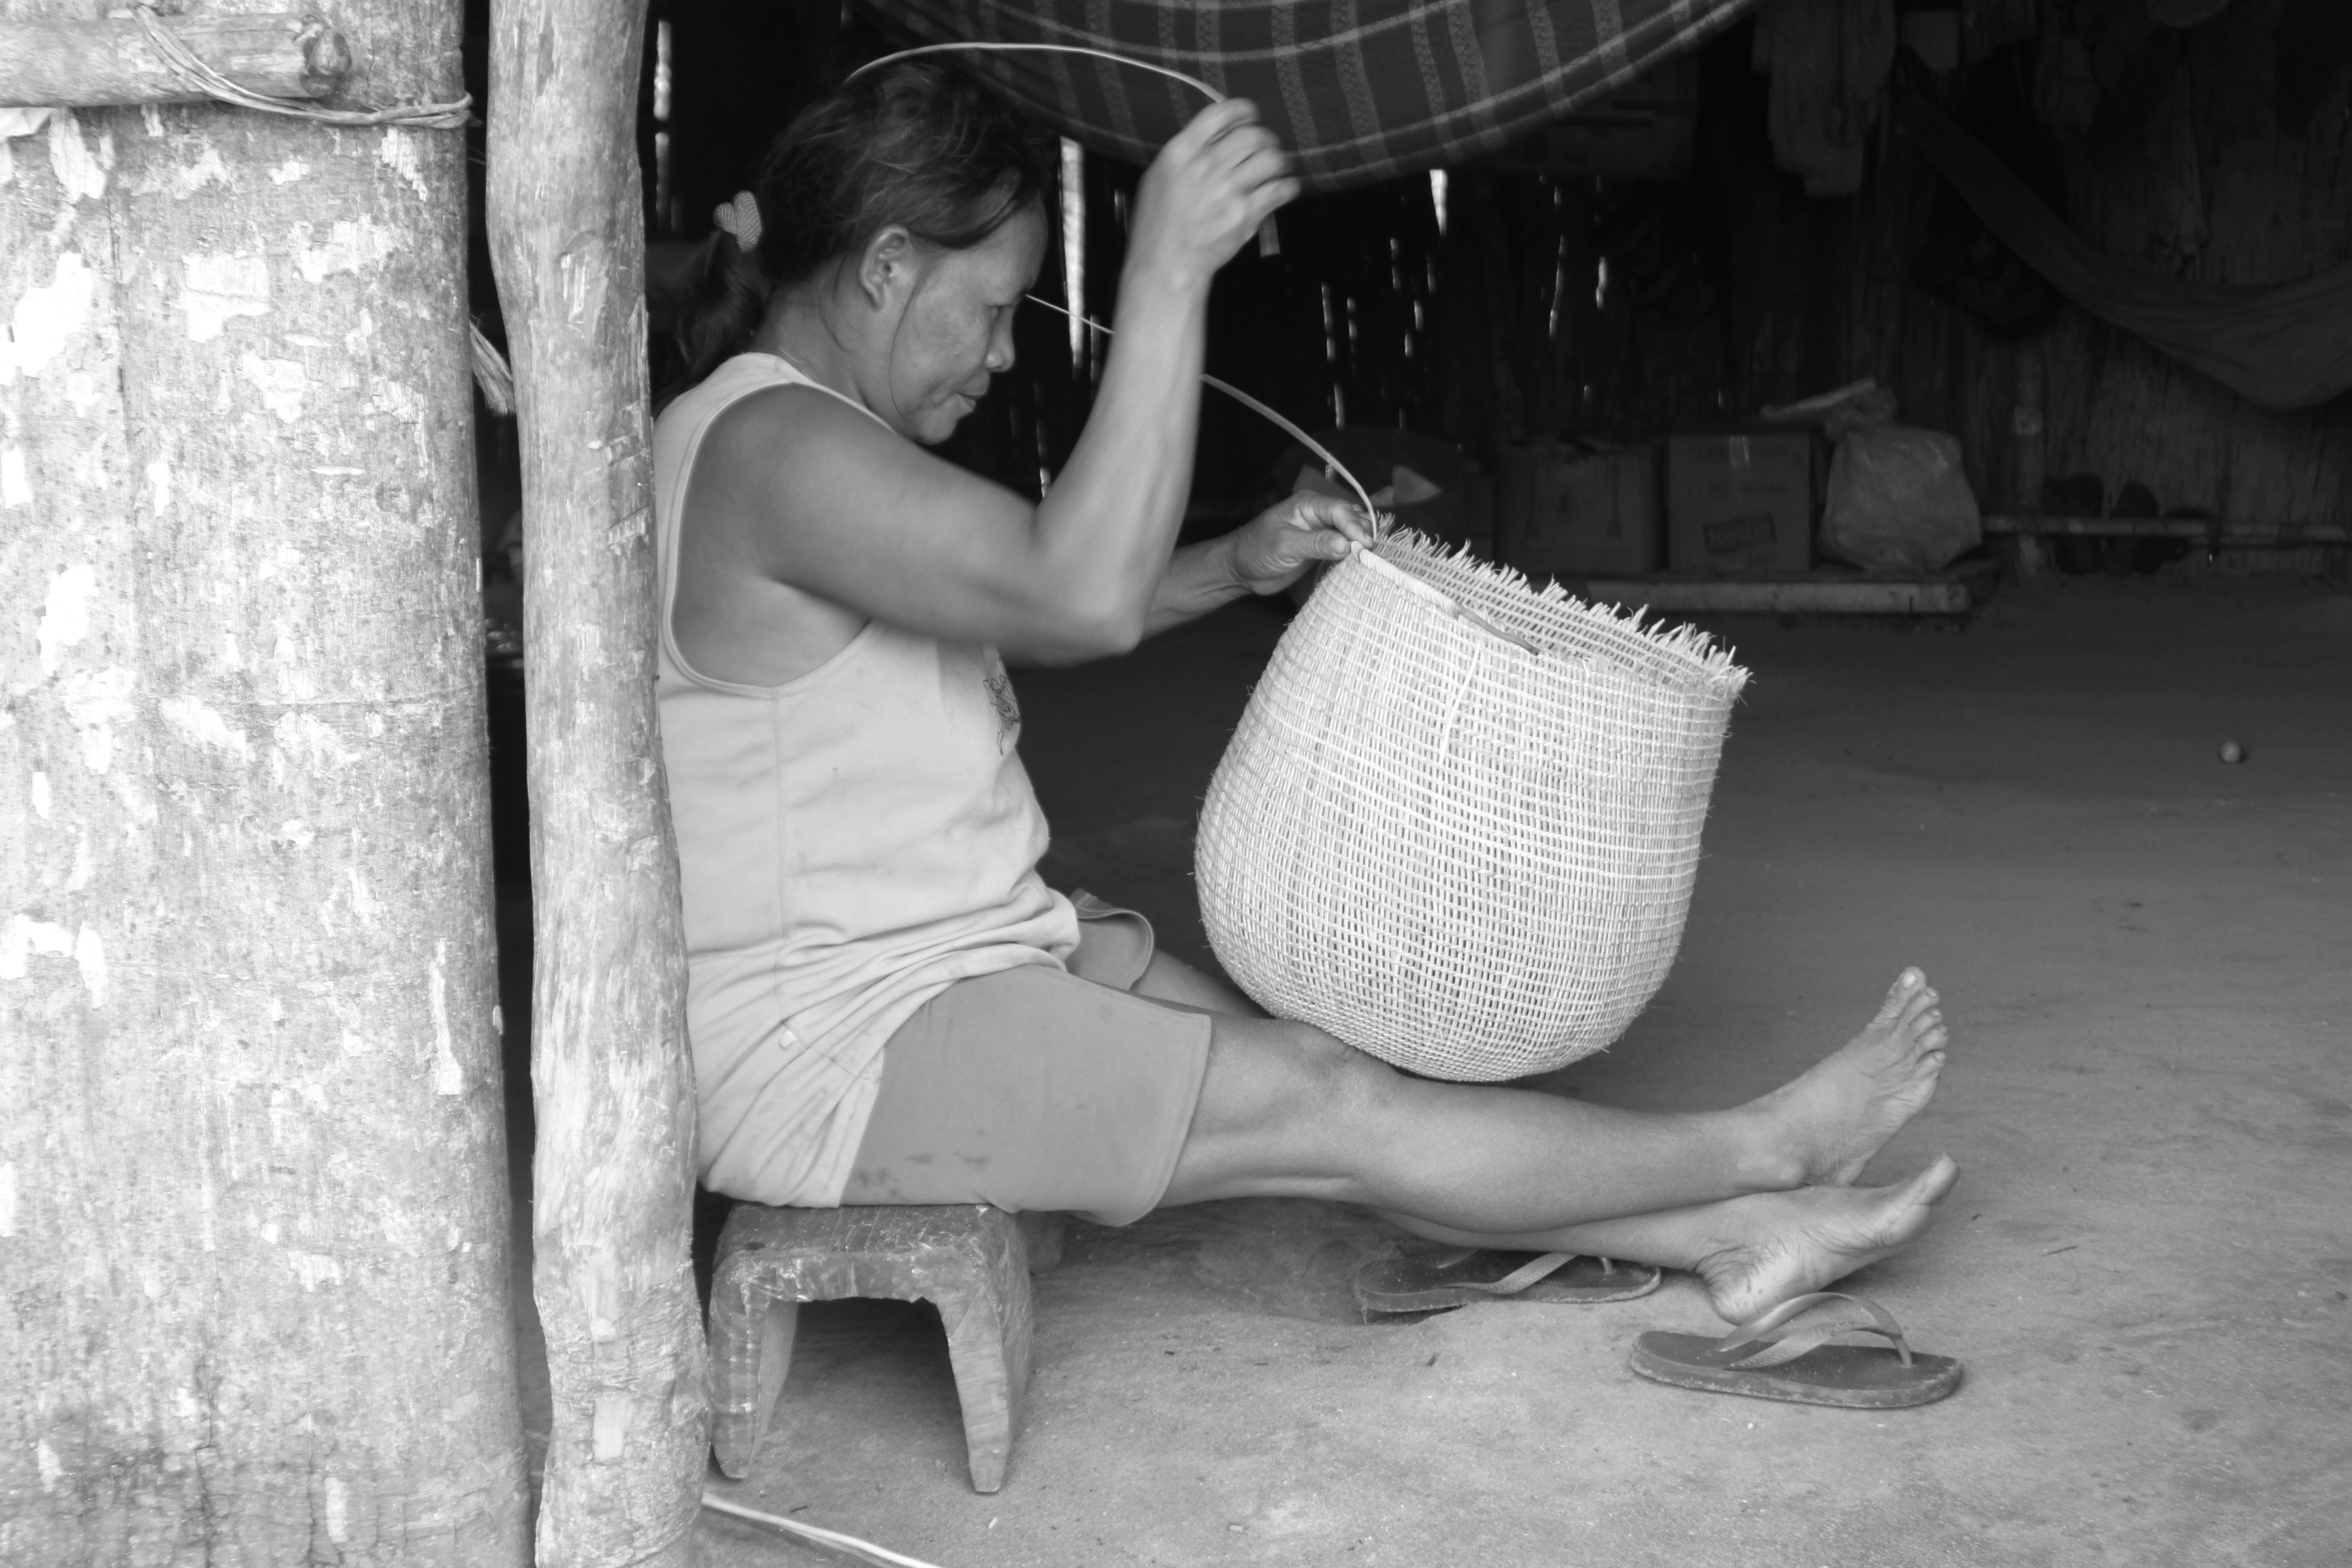
\includegraphics[width=\textwidth]{./img/022}
%\caption{Isabel terminando um aturá (foto: Danilo Paiva Ramos, 2012)}
%\end{figure}

Com o crescimento corporal, os aturás e os arcos e flechas aumentam de
tamanho, os meninos e a meninas tornam"-se mais hábeis para construí"-los.
Os meninos adquirem melhor mira e tônus muscular, enquanto as mãos
femininas passam a tramar com rapidez e leveza. No menino, o arco e
flecha presente nos braços aumenta de tamanho, mas seu aturá mantém"-se
pequeno, enquanto na menina o cesto cresce, mas o arco e flecha
permanece pequeno. Fabricando seus arcos e flechas, brincando com eles
ao acompanharem os pais, os meninos desenvolvem habilidades ligadas ao
braço, às mãos e às pernas que contribuem para o crescimento de seus
artefatos internos e para a sua socialização como homens. Sentadas
tramando os fios de arumã ou seguindo as mães carregando seus cestos, as
meninas fazem a si mesmas, agem sobre sua corporalidade, tornam"-se
habilidosas artesãs e fortes carregadoras.

Desacompanhado de sua mãe, o pequeno tamanduá manejava precisamente suas
lâminas e garras, mas não conseguia a mesma eficácia no uso de seu
rabo, que é um remo, para a fuga, o que aponta para sua condição de noviço, que,
como as crianças hup, é introduzido aos poucos pela mãe em contextos
para o uso de suas armas e instrumentos corporais. Como ressalta
Hugh"-Jones (2009, p.\,48-9), ``se as pessoas são progressivamente
construídas e socializadas como montagens de objetos, também os objetos
podem socializar pessoas {[}\ldots{}{]} Fazer coisas é, assim, fazer a
si e a maestria da técnica é a maestria do eu''.

Os golpes de terçado precisos foram dados no focinho, \textit{tö̖j"-moy}, e no
pescoço, \textit{k'atɨ̗t"-moy}, dos tamanduás. A mira dos arqueiros visa sempre
atingir o peito, \textit{hãg"-sa̗k moy}, das presas, uma técnica muito eficaz
principalmente na caça a grandes mamíferos como o tamanduá, a anta, os
porcos e os catetos. O caçador evita, desse modo, os membros, onde estão
as armas primordiais e corporais (garras) dos animais, para atingir seus
órgãos vitais. No encontro da caça, as facas (garras), espadas (garras)
e remos (rabo), manejados pelas presas para o enfrentamento e fuga, são
igualmente armas primordiais que lhes permitem defender"-se e atacar.
Assim, os corpos humanos e animais podem ser observados como
\emph{composições artefactuais} que indicam as habilidades, forças e
estruturas possuídas por cada ser. Como o filhote de tamanduá, as
crianças hup também têm suas armas, adornos e utensílios corporais.

Acredito que a designação de partes do corpo como artefatos, armas e
instrumentos expressa a habilidade de alternância entre a \textit{ɨ̗d},
``fala'', e a \textit{bi'i̖d ɨ̗d}, ``linguagem de benzimento''. Essa alternância
entre gêneros discursivos é também a alternância entre modos de
percepção da corporalidade do ser. Parece haver um paralelismo entre a
aquisição de habilidades no uso e fabricação de armas e instrumentos
pelo noviço e seu desenvolvimento físico"-motor com o seu crescimento.
Pensando com McCallum, a produção desses artefatos depende do
desenvolvimento de \textit{corpos que sabem}. Produzir seria, assim,
transmitir aquilo que o corpo sabe para o objeto produzido, permitindo
que o próprio objeto no curso do uso pela pessoa, humana ou animal,
molde as partes do seu corpo fazendo crescer os artefatos primordiais e
as habilidades. Os objetos têm, assim, graus relativos de materialidade
aos quais caçadores e xamãs se referem através de uma alternância
perspectiva da percepção que faz os corpos surgirem como composições
artefactuais vivas em dados contextos relacionais.

\section{O arco e o cesto}\label{o-arco-e-o-cesto}

Na noite de 17 de março de 2012, depois da roda de coca, voltei para a
casa de Américo, onde eu estava alojado. Abri a porta com cuidado, pois
as crianças e meus anfitriões pareciam já estar dormindo. Acendi minhas
velas, abri meu caderno de campo e, quando ia começar a escrever,
Isabel, que amamentava a pequena Creuza, perguntou se eu já conhecia o
\textit{benzimento do filho}. Como minha esposa estava grávida, era muito
importante que eu soubesse executá"-lo. Filha de um pajé de \textit{Pi̖j"-Dëh},
minha anfitriã descreveu algumas ações do encantamento que havia
aprendido com seu pai. Mãe de seis filhos, Isabel alertou"-me
principalmente quanto aos perigos do contato dos pais com alguns objetos
durante o resguardo. Para ela, a febre de Tereza e da recém"-nascida
tinham sido causadas por Elias ter \textit{pego em máquina}, ou seja, ter
dirigido a rabeta durante a navegação de retorno de São Gabriel.

A mulher não pode pegar em \textit{ma̗j}, ``aturá'', senão a criança terá doença
nos olhos. Se o pai pegar em máquina, a criança morrerá. O contato com o
arco e flecha fará o umbigo do bebê sair. É perigoso também que os pais
peguem em terçado, pois o filho pode ter \textit{Pu̖ç Way}, ``umbigo saído''.\footnote{Caderno de campo, 17 de março de 2012.}

\index{ag@\textsc{b}6\quad \textit{Te͂h Bi'i̖d}\break Benzimento do filho}
Após o nascimento, os pais devem ficar na rede. Além do jejum, é
necessário que o casal não toque em instrumentos de trabalho ou armas.
``Então, eu sopro a cuia de beber mingau da mulher. Se quiser, ela fica
um dia parada e já está bom'', explica Ponciano em \textsc{b6}. A
restrição do tato é também uma contenção dos movimentos que devem tender
à imobilidade. Como na dieta alimentar, o manuseio dos objetos acompanha
a restituição gradual dos deslocamentos. Com o tempo, o casal começa a
poder visitar as casas vizinhas, participar das rodas de conversa até
que, ao término do resguardo, possam finalmente caminhar para a roça,
mata ou igarapé. Pouco depois, a mulher pode manusear os cipós de arumã
e tramar os cestos de aturá. O marido pode igualmente dedicar"-se ao
artesanato de tipitis, cumatás e, posteriormente, arcos e flechas,
objetos produzido exclusivamente pelos homens. Os cipós são trazidos
pelos parentes. Os objetos fabricados pelo casal são trocados com outras
famílias por farinha, beijus e peixes.

A mobilidade dos parentes garante, assim, a reintrodução do casal aos
movimentos corporais. As mãos tramam os fios, os olhos acompanham os
nós. Deitados nas redes por muitos dias, os pais começam agora a
sentar"-se e a mover os braços sem ainda tocar utensílios ou armas. As
trocas de artesanatos com os parentes garantem uma quantidade
complementar de alimentos que, preparados pela acompanhante e benzidos
pelo xamã, resfriam e nutrem os corpos. Como no aprendizado da criança
sobre a fabricação de seus \textit{brinquedos}, o artesanato vai, através da
produção dos objetos, ressocializando o casal nas habilidades manuais
específicas de cada gênero. Fazendo os objetos, pai e mãe refazem"-se a
si mesmos como homem e mulher hup, ao mesmo tempo em que, pelo tato e
pela visão readquirem a precisão de seus movimentos. Pensando com
Deleuze e Guattari, nesse momento de restrição dos movimentos, os pais
seguem os cipós e as madeiras no fluxo de suas matérias, em suas
itinerâncias conforme fazem crescer seus artefatos,

\begin{quote}
De qualquer modo, trata"-se de seguir a madeira, e de seguir na madeira,
conectando operações e uma materialidade, em vez de impor uma forma a
uma matéria: mais que a uma matéria submetida a leis, vai"-se na direção
de uma materialidade que possui um nomos. Mais que a uma forma capaz de
impor propriedades à matéria, vai"-se na direção de traços materiais de
expressão que constituem \emph{afetos}.\footnote{1980, p.\,96.}
\end{quote}

Isabel alerta que a mãe que pega em aturá deixa os olhos da criança
\textit{mi͂gi͂}, ``loucos''. O pai que pega em arco e flecha ou terçado faz o
umbigo do bebê sair. Enquanto o arco e flecha e o terçado são armas
manejadas pelo caçador em seus combates com as presas, o aturá é o cesto
de carga que acompanha a mulher em praticamente todos os seus afazeres.
Como na produção do artesanato, o caçador com seu arco e flecha e a
agricultora com seu aturá às costas seguem com uma \textit{identidade vaga}
entre os corpos e as coisas. Seguem como matéria"-fluxo"-movimento na
sinergia entre os artefatos corpóreos primordiais, o peso do cesto às
costas e o volume do arco oprimido pela pressão da mão cerrada. São
assim conjuntos vagos que ``desprendem uma corporeidade (materialidade)
que não se confunde nem com a essencialidade formal intangível, nem com
a coisidade sensível, formada e percebida''.\footnote{Deleuze; Guattari, 1997,
p.\,95.} Dirigem"-se a contextos de agenciamento que se dão no encontro
com o animal e na lida com as manivas da roça, contextos plenos de
energia quente e agressividade que se impregnam em seus corpos"-objetos.

No encontro com o animal, o caçador hup maneja suas armas, facas e arcos
e flechas. Empunhadas externamente em suas mãos, as armas são também
parte constitutiva de seus membros corporais. A agressividade dos
combatentes, considerada como um calor excessivo, impregna"-se nos corpos
do predador e da presa. O arco e flecha ou o terçado incandescente faz
arder os braços do caçador. Chegando à sua casa, o caçador pendura logo
suas armas nos caibros do telhado de caranã e come pimenta para atenuar
a agressividade que o combate despertou em si. De forma semelhante, as
garras, dentes, cartilagens ou ossos espinhosos do animal abatido estão
plenos de agressividade e precisam logo ser descartados porque podem
ainda ferir o caçador ou sua família durante o consumo. A carne dos
animais precisa ser bem cozida com pimenta para impedir o ataque onírico
da vítima com suas armas primordiais, facas, espadas e cuias de \textit{caarpi}.

Durante a \emph{couvade}, ao tocar as suas armas ou ao ingerir a carne
não benzida, o pai faz sair o umbigo do recém"-nascido. Para a cura, o
xamã sopra uma colher de aço, objeto frio que, ao entrar em contato com
o umbigo, reverte sua dilatação e putrefação, endurece e resfria o
\textit{molengo} na parte que antes era o local de ligação materno"-fetal pelo
cordão"-umbilical. Esse aquecimento das armas e membros do caçador parece
análogo ao calor que a condução da rabeta, uma máquina, faz aderir ao
corpo do navegante. No caso de Elias, segurar a máquina quente foi a
causa da febre em sua esposa e na bebê recém"-nascida. Assim, o manejo de
arcos e flechas, terçados e motores parece impregnar o calor dos objetos
presentes no corpo do pai que, por sua vez, transfere essa intensidade
térmica e destrutiva ao corpo do filho. A melhora da febre ocorre com os
banhos, ingestão de frutas e repouso, ou seja, no contato do corpo com
essências frias.

Como contou certa vez Ari, é no peito, morada do \textit{hã̗wäg} e do \textit{b'atɨ̖b'},
que está situado o calor do corpo. Já o frio se encontra espalhado pelo
resto do corpo. Para verificar"-se a febre, coloca"-se a mão na testa, nos
braços e nas pernas, pois a doença faz espalhar o calor desse centro
vital para as extremidades corporais. Além do aquecimento da cabeça e
peito, quando estão com ``febre'', \textit{pë' wɨd ne̖n}, os Hupd'äh dizem ver
cores, manchas luminosas que os olhos começam a perseguir de modo
perturbado. O equilíbrio entre o frio das extremidades e as energias do
sopro vital, essencialmente frio, e da sombra, essencialmente quente, é
o que garante um estado saudável ao corpo. \textit{Mɨnɨ̗g këy}, ``ver direito'',
é também ver reto como o pensamento que \textit{mɨnɨ̗g ha̗m}, ``segue reto'',
algo que remete a um movimento \textit{retilíneo} ou \textit{focado} dos olhos.
\textit{Mi̗͂gi̗͂}, ``louco'', é a pessoa cujo pensamento se encontra espalhado.
Desloca"-se em muitos sentidos, mas não consegue concentrar"-se e seguir
um caminho. A febre que causa \textit{Käwä̖g mi̗͂gi̗͂}, ``olhos loucos'', faz os
olhos perderem o rumo, movimentarem"-se a esmo e perseguirem cores
espalhadas pelo espaço.

\index{ag@\textsc{b}6\quad \textit{Te͂h Bi'i̖d}\break Benzimento do filho}
Na roça, o aturá fica exposto ao sol por muito tempo, enquanto a mulher
trabalha a maniva. Nesse sentido, pegando"-o ou carregando"-o, a mulher
toca um objeto externo que se apoia sobre sua estrutura lombar, composta
por seu cesto primordial. Em \textsc{b6}, o xamã faz com que \textit{Wero̗ Hup
Te͂h i͂h}, o Sol, suba para sua morada celeste, apague sua lenha
corporal, largue sua faca e volte seu olhar para cima. Como visto, o
odor dos corpos da mãe e do bebê ofende esse ancestral que se vinga
através de sua luz e calor. O objeto pessoal e de carga da mulher
torna"-se o vetor da agressividade desse ser, que leva os corpos já
quentes da mãe e do bebê a arder em febre, e os olhos, a enlouquecer.
Nos termos de Buchillet, a doença causada pelo toque do aturá é um modo
de feitiço indireto causado pela ação maléfica do sol. Nas palavras da
antropóloga:

\begin{quote}
A segunda forma de feitiçaria consiste em alterar um objeto que pertence
a, ou que é utilizado pela pessoa que se pretende agredir, recitando um
encantamento sobre esse objeto: o mal é assim transferido ao indivíduo.
Como em numerosos grupos indígenas, os Desana postulam uma ligação entre
um indivíduo e seus pertences (vestes, utensílios, etc.) como
continuidades de si em efeitos pessoais ou nos objetos que ele utiliza.\footnote{Buchillet, 1983, p.\,137.}
\end{quote}

Da mesma forma como o sopro das palavras faz com que as ações \textit{hã̗wägät}
do xamã se condensem no cigarro para depois, quando inspiradas, agirem
no corpo da pessoa, creio que por meio do aturá ou das armas de caça, o
calor e a agressividade frutos da exposição à ação do Sol ou ao ardor
das batalhas impregnam"-se nos objetos, próteses externas e, ao mesmo
tempo, artefatos que compõem o corpo. O bebê, um molengo, em contato
permanente com os pais, é exposto a essas energias, que intensificam a
presença de \textit{k'ɨ̗}, ``calor'', em seu corpo, ocasionando a febre, a
perturbação ocular, a saída do umbigo e a abertura de feridas. O toque
dos objetos é um \emph{acontecimento"-afeto} que faz os agenciamentos
das armas e instrumentos convergirem dos pais para o bebê através do
fluxo existente entre a pessoa e os corpos"-objetos, conjuntos vagos de
matéria"-movimento, matéria"-energia e matéria"-fluxo.

\index{24@\textsc{m}15\quad \textit{Bisi̗w}, o devorador de rapazes}
Em \textsc{m15}, \textit{Bisi̖w}é vencido pelos pais vingadores ao beber o
caxiri soprado. Aceitando o oferecimento, ele toca um recipiente grande
de argila, uma \textit{bok tãw}, e bebe o líquido que o embriaga rapidamente.
Bêbado, \textit{ä̗g na̗' yɨ̗'ɨ̗y}, ele cai no chão. Os pais colocam"-no sobre a
lenha e o queimam. A ardência faz seu corpo desarranjar"-se. Seu corpo
\emph{artefactual} fragmenta"-se e surgem as flautas Jurupari, seus
ossos. Antes de morrer ele pragueja ameaçando fazer com que os Hupd'äh
sofram como ele sofreu. Algumas doenças que acometem os Hupd'äh derivam
dos sofrimentos que os antigos causaram a \textit{Bisi̗w}. Nesse sentido, o
canibalismo anal, que aniquila os rapazes, pode ser visto como uma
primeira ação de roubo do espírito para o consumo predatório. Se o fogo
que queima \textit{Bisi̗w} desconstrói seu corpo, fragmentando sua pessoa
corporificada em múltiplas flautas singulares, as doenças que acometem o
recém"-nascido parecem também desconstruí"-lo pela intensidade extrema de
calor.

A febre e o choro enlouquecedor atestam a viagem do recém"-nascido como
pessoa"-sopro que pode ter sido devorada por seres malfazejos. A saída do
umbigo mostra"-se uma dilatação, ou putrefação, no local que antes era a
ligação com a mãe. As feridas, aberturas corporais, podem também ser
vistas como tensões d fragmentação ocasionadas pela pele mole,
decompondo"-se. Sem estar duro o suficiente para suportar o ataque
onírico de seres como as Gentes"-Árvore, \textit{B'atɨ̖b'}, ou a vingança das
presas e peixes consumidos pelos pais que ferem com suas armas
laminares, as feridas abrem"-se e custam a fechar. Podem ocasionar dores
terríveis e agravar"-se como no caso da leishmaniose. A cuia de \textit{caarpi}
oferecida por insetos (como os bichos do pé), ou por animais consumidos
(como o tamanduá) são causas do choro enlouquecedor, que pode ocasionar
febres, umbigo saído e olhos perturbados. Pensando com Lolli (2010,
p.\,29), a exposição do bebê a essas afecções de outrem por intermédio de
seus pais revela, ``na doença, o caráter duplo de construção e de
desconstrução da função xamânica que se mostra mais patente, à medida
que concomitantemente implica de um lado a recuperação do doente e do
outro a desconstrução dos agentes patogênicos''.

Segundo McCallum,\footnote{1998, p.\,217.} o corpo é ``afetado e construído por
diferentes processos materiais que ocorrem perto ou dentro de seus
corpos, como no \emph{couvade} e nas `relações de substância' de forma
mais geral''. Durante o resguardo, a \emph{consubstancialização} entre
os pais e o bebê faz com que os movimentos, o tato e a dieta incidam
sobre a corporalidade, sentidos e o pensamento do recém"-nascido, que
pode sofrer com o \textit{umbigo saído}, o \textit{choro enlouquecedor}, as febres
ou as feridas abertas. As enfermidades causadas pelo tato indevido
parecem colocar em risco o processo de endurecimento corporal do
\textit{molengo}, fazendo com que, devido ao aquecimento, os olhos se
perturbem e percam seu foco, o umbigo dilate"-se e saia, a pele se abra
em feridas e o sopro vital deixe o corpo.

\section{O feto adornado e o dono dos
animais}\label{o-feto-adornado-e-o-dono-dos-animais}

Numa roda de coca, conversando sobre o benzimento do filho, Ponciano me
contou que, no útero, além de comer coca como os velhos, o ``feto de
sexo masculino'', \textit{tiyi̖'}, está armado com seu arco e flecha e com sua
zarabatana. Em sua cabeça, ostenta um lindo cocar colorido feito com
penas de arara e papagaio. Recobre sua nuca com o \textit{wi̖h huj}, ``cocar de
penas de gavião''. Em seus braços, tem pulseiras de tucum, suas \textit{K'ö̖b
s'o̗} e \textit{K'ö̖b hikub}. Sua perna vibra ao som de seu \textit{yã̖ç}, ``chocalho de
pé'', a cada passo de dança. Carrega, às costas, um pequeno cesto aturá.
Já a menina, \textit{tã'ã̗y}, decora seus cabelos pendurando uma ``flor'',
\textit{s'o̗}, na orelha. Carrega às costas seu grande aturá para levar a
maniva. Para o preparo do caxiri, a menina traz consigo seu ``ralador'',
\textit{hɨ̗p}, seu ``balaio'', \textit{pa̗'}, e seu suporte de cumatá, \textit{moho̖y}. Além dos
instrumentos de trabalho, está munida de um arco e flecha e uma
zarabatana pequenos. Os meninos têm as faces pintadas de preto. As
meninas, de vermelho. Ambos estão sentados sobre seus ``bancos de
nascimento'', \textit{hib'a̗h kä̗d}. Seguram firme seus ``bastões'', \textit{sö̖h tëg}, e
têm as ``sementes de pedra'', \textit{pa̖ç wäg}, penduradas em seus peitos.

Adornados dessa forma, assemelham"-se aos antigos em pleno Dabucuri
quando, dançando, manejavam as potências primordiais. Pensando com Gow,
os fetos adornados são \emph{agentes de seu próprio nascimento}, nas
palavras do autor sobre os Piro, ``o genitor e a genitora são os agentes
de seu vir a ter corpo; o feto é o agente de seu próprio nascimento.
Os bebês `surgem de dentro' ativamente; eles não são passivamente
`paridos' ou `dados à luz'''.\footnote{Gow, 1997, p.\,47.}

Os encontros cerimoniais entre moradores de aldeias distintas de um
mesmo grupo local para realizar trocas rituais de alimentos por caxiri
recebem, em língua hup, o nome de \textit{Pä̗'}, ``derramar'', que são os
\textit{Dabucuris} uaupésinos em língua geral. Trazendo cestos carregados com
frutas, carnes ou peixes, os \textit{convidados} derramam suas dádivas no
centro da maloca, ofertando"-as a seus anfitriões. Enunciados formais de
agradecimento e exaltação dos parceiros de troca acompanham o gesto de
derrama dos aturás e de recebimento das cuias de caxiri dadas pelos
\textit{anfitriões}. Esses encontros criam as condições para que ocorra a
iniciação masculina com a exibição das flautas \textit{döhö̗ d'äh},
Jurupari, aos neófitos, que começam a aprender a soprá"-las para
trazer à vida os ancestrais clânicos. Devido aos perigos que envolvem
essa prática, as mulheres e as crianças têm que permanecer isoladas na
mata para não verem as flautas que são, simultaneamente, os ancestrais e
os ossos do terrível \textit{Bisi̗w}.

Ainda hoje, momentos antes da realização do evento, os senhores hup
começam a comentar nas rodas de coca a \textit{queda das frutas},
referindo"-se à maturação do ingá, do ucuqui, do uacu, etc. que atraem os
animais. Em plena fartura, as pacas, cotias, tamanduás realizam danças e
cerimônias de trocas em \textit{Hu̗͂-Mo̖y }, a Casa"-dos"-Animais, junto ao seu
dono, \textit{Bisi̗w}. Esse é o momento de formar grupos para colher grandes
quantidades de frutos, abater um número substancial de presas, e/\,ou
tinguijar os igarapés. Os donos hup designam representantes para viajar
à aldeia dos parentes distantes para combinar a celebração. Realizados
secretamente na década de 1970 devido ao temor da repressão salesiana,
os \textit{Pä̗'} dos Hupd'äh não puderam ser observados por Reid, que escreveu
as seguintes notas sobre o ritual:

\begin{quote}
Durante os rituais formais, as crianças, meninos e meninas, são
obrigados a deixar a maloca e a manterem"-se afastados quando os
trompetes Jurupari entram na maloca. Entretanto, com aproximadamente 9
anos, os jovens são expostos aos trompetes pela primeira vez.
Disseram"-me que esse é o evento que marca formalmente a transição da
infância à idade adulta. {[}\ldots{}{]} As cerimônias rituais de troca
praticadas pelos Hupdʉ são denominadas \textit{Pwu!}, que significa derramar.
{[}\ldots{}{]} Essas cerimônias geralmente envolvem o uso dos trompetes
sagrados, que possuem diversos nomes em Hupdʉ. Desse modo, em rituais
formais, os jovens não somente performam e aprendem como tocar os
trompetes sagrados, mas também a dançar corretamente. Além disso,
recebem orientações dos anciões em mitologia e cantos. {[}\ldots{}{]}
Muitos dias antes da realização dos rituais, os homens Hupdʉ vão à
floresta para caçar ou coletar frutas silvestres demandadas, enquanto os
Índios do Rio preparam o caxiri, o tabaco e a coca. {[}\ldots{}{]} Na
alvorada, após algumas horas de descanso em seus cantos, os Hupdʉ
começam a apresentação das frutas aos anfitriões, vestindo suas melhores
roupas e tendo o rosto pintado. Eles dançam em linha até a maloca, e
após sequências de dança e consumo de bebida, depositam suas dádivas no
centro da maloca.\footnote{Reid, 1979, p.\,151-2; 181-2.}
\end{quote}

Para descrever os pertences dos seres intrauterinos, Ponciano remetia"-se
sempre às antigas cerimônias de Dabucuri que havia presenciado. Cores,
sons e gestos dos pais e avós teciam as linhas dessa memória ritual, que
fazia um imenso sorriso abrir"-se nos lábios do xamã. Ele explicava que a
tinta que colore os rostos dos nascituros é preparada com a mistura da
planta \textit{yawi̖'}, ``samambaia'' (tipo de), com a semente de \textit{me̖'},
``carajuru'',\footnote{\textit{me̖'}, ``carajuru'', planta cujas folhas produzem
  uma tinta vermelha para untar o rosto quando misturadas com urucum.
  Família da bigniniáceas, \emph{Arrabidae chica}. Cf. Ramirez (2006).}
para a pigmentação vermelha, ou com ``jenipapo'', \textit{d'a̖d}, para obter a
cor negra. ``Era assim que os antigos pintavam seus rostos para os
Dabucuris antes'', lembrava"-se. O ancião trouxe um \textit{yãç}, ``chocalho de
pé'', que havia fabricado depois de nossa caminhada à Casa"-dos"-Animais.
Colhera as castanhas enquanto caminhávamos. Para mostrar"-me o
instrumento que os fetos masculinos amarram em seus tornozelos, Ponciano
levantou"-se e começou a bater o pé no chão. Próximo à roda de coca,
segurando uma vassoura, ele dançou como se soprasse uma flauta Jurupari
e transformou o encontro noturno num Dabucuri.

Em eventos de iniciação, quando as flautas Jurupari terminam de ser
tocadas e exibidas aos rapazes, iniciam"-se os bailes e o oferecimento
generalizado de caxiri. As flautas Jurupari silenciam à beira do
igarapé. Os músicos desmontam seus instrumentos e enterram"-nos no leito
do córrego. As mulheres começam a circular as panelas de caxiri e as
crianças voltam a correr pela aldeia. As flautas cariçu são trazidas e
os chocalhos amarrados aos tornozelos dos dançarinos. As moças,
inicialmente sentadas na metade feminina da maloca, levantam"-se,
dirigem"-se a um dos flautistas e apoiam a mão no ombro do músico.
Juntam"-se ao corpo de baile que segue fazendo movimentos circulares e
zigue"-zague pela área central.

No útero, é a partir dos movimentos de dança do feto que o xamã percebe
o sexo do bebê. Se, ao soprar o cigarro, o benzedor sentir uma pressão
em seu tornozelo, a sensação indica haver um chocalho de dança masculino
amarrado à canela da criança. Do contrário, se sentir uma mão apoiada no
ombro do xamã, o bebê será uma menina. Após o nascimento, as mulheres
cantam \textit{yamido} e dançam no terreiro descrevendo passos de ``cariçu'',
\textit{hëhë}, para ninar a criança ou consolá"-la. Enquanto o xamã faz par com
a menina, seu corpo identifica"-se ao do nascituro menino.

Antigamente, pouco antes da chegada dos convidados, iniciavam"-se os
preparativos para o Dabucuri. Os \textit{convidados} formavam grupos de
viajantes e rumavam para as cabeceiras. Caçando e pescando, buscavam as
aves com cujas plumas adornariam seus corpos. Araras e papagaios
forneciam as penas azuis e vermelhas para a confecção dos \textit{yak pãt},
``cocares''. Já os cocares de nuca eram feitos com as penas dos ferozes
gaviões que habitam os morros, demonstrando a valentia de quem os
portasse. Podiam também ser organizadas grandes expedições de caça, ou
até mesmo a retirada de timbó para tinguejar os igarapés e obter grande
quantidade de peixe. Com a fibra do tucum, preparavam"-se os fios para a
confecção de pulseiras de braço e enfeites como braceletes e colares.
Para atrair as mulheres, os rapazes esfregavam pussangas, plantas com
odores agradáveis que os ajudavam na sedução. As flores que enfeitavam
as orelhas das moças podiam estar igualmente preparadas para atrair
parceiros. Ainda hoje, devido à imensa quantidade de caxiri ingerida
durante os Dabucuris, as mulheres passam os dias anteriores carregando
aturás cheios de maniva. Usam seus ``ralos'', \textit{hɨ̖p}, para extrair a
massa que depois é espremida nos cumatás para obter a manicuera.

O feto adornado parece fazer convergir para a gestação modos de ação
característicos dos Dabucuris. A transmissão de bens, adornos e
instrumentos corporificam potências primordiais. Esse processo ganha
expressão com as danças performadas durante os Dabucuris. Os gestos e
movimentos expressam as capacidades, intenções e responsabilidades que
poderão transformar os fetos em humanos em ancestrais e, reversamente,
regenerar o ancestral pelo novo ser. Agentes de seu nascimento, ao longo
do desenvolvimento uterino, os nascituros preparam"-se para a interação
com o \textit{avô xamã}, que, como Ponciano, lembra"-se de cada detalhe dos
adornos rituais dos antigos. Os fetos adornados surgem com seus
pertences que são também índices diacríticos de seus sexos e posições no
campo de interações rituais. Uma espécie de devir ancestral faz sua
pintura e adornos identificarem"-nos aos \textit{antigos} e aos \textit{velhos}.
Sentados diante de um Lago de Leite, os fetos são os próprios ancestrais
a receber de \textit{K'e̖g Te͂h} os ossos, ou flautas, de \textit{Bisi̗w}, os Jurupari, junto
com os demais bens e alimentos da origem (\textsc{m15}).
\index{24@\textsc{m}15\quad \textit{Bisi̗w}, o devorador de rapazes}

Às vésperas do Dabucuri, alguns mentores ainda levam os grupos de
rapazes para colher frutas como cucura, ucuqui, uacu, pupunha e ingá nas
roças do \textit{Bisi̗w}, espalhadas pela mata. Aqueles que estão prestes a ver
os ossos-flautas desse ancestral, queimados pelos antigos hup, precisam
caçar as presas liberadas pelo dono e colher as frutas por ele cedidas.
Para isso, os xamãs realizam viagens prévias à \textit{Hu̗͂-Moy}, para oferecer
sopros vitais e/\,ou tabaco como dádivas a \textit{Bisi̗w}. Todo o cuidado é pouco
para que os jovens hup não tenham seus sopros vitais devorados por esse
terrível predador. O ritual de troca entre grupos hup, \textit{pä̗'}, e a
iniciação masculina, \textit{döhö̗}, dependem, assim, do estabelecimento da
reciprocidade adequada com esse ancestral. Ao mesmo tempo, os animais
bebem, cantam, dançam e copulam no interior da \textit{Hu̗͂-Moy}, realizando seus
próprios Dabucuris para que os Hupd'äh possam, posteriormente, também
celebrar, \textit{procurar filhos} e transformar seus rapazes em homens
fortes.

\index{ag@\textsc{b}6\quad \textit{Te͂h Bi'i̖d}\break Benzimento do filho}
Enquanto o \textit{avô benzedor} convence o feto, sentado, a entregar seus
pertences (\textsc{b6}), os xamãs devem convencer \textit{Bisi̗w} a regenerar as
presas e libertá"-las para saírem para a floresta. Essa ação
\textit{diplomática} instaura a reciprocidade entre um avô e seu neto e entre
um ancestral e seus descendentes. Evocando o nome de um antepassado
clânico, o avô concentra a pessoa distribuída do neto, ou ancestral.
Soprando as flautas enquanto dançam, os netos reúnem os ossos, os
fragmentos de \textit{Bisi̗w} num corpo de dança, trazendo à vida o ancestral
para crescerem, endurecerem seus corpos e protegerem"-se das doenças.

Se, comendo a coca, os senhores hup predam os ossos e a carne do Velho
Cobra, e assumem a perspectiva de \textit{We̗d B'ö̖'}, o nascimento insere o bebê
num processo gradativo de oferecimento de alimentos, algo que aproxima
os bebês da pessoa de \textit{We̗d B'ö̖'}, o irmão maior de \textit{Bisi̗w}. É preciso
lembrar que esse primogênito não conhecia os alimentos próprios como
beiju, peixe moqueado, caxiri, coca, tabaco etc. Progressivamente, os
alimentos das Gentes"-Cobra vão sendo oferecidos a ele por uma Mulher
Peixe, sua esposa. De seu vômito surgem os alimentos próprios e as
plantas domesticadas. Ao longo de \textsc{b7}, para tornar os alimentos
próprios, o xamã manda os animais para suas moradas ancestrais e cerca
suas armas para que as presas não se vinguem daquele que preda seus
corpos. Seguindo Århem,\index{ah@\textsc{b}7\quad \textit{B'a' Bi'i̖d} \break Benzimento do Beiju}

\begin{quote}
Conforme o benzedor dos alimentos remove a \textit{armas} da comida e
manda"-as de volta a sua origem, ele performa um ato essencialmente
regenerativo: faz retornar a \textit{alma} do animal morto e cozido (ou da
planta comestível) para sua casa de nascimento e, por meio disso,
permite seu subsequente renascimento.\footnote{Århem, 1996, p.\,197.}
\end{quote}

A morte do animal é, como para os humanos, uma fragmentação de seus
princípios vitais com o retorno de seu sopro vital à morada primordial.
Numa conversa, Américo disse que \textit{Bisi̗w} chama os animais para juntá"-los
novamente. Seu grito, que pode ser ouvido pelos caçadores a ecoar pela
mata, concentra novamente os princípios vitais das presas abatidas,
regenerando a vida. A reunião dos animais suscitada por seu chamado é,
assim, a concentração de seus seres tornando"-os vivos novamente. Plena
de Dabucuris, a Casa"-dos"-Animais assemelha"-se a uma maloca onde a dança
e o sopro das flautas fazem surgir \textit{lagos de leite}. A predação constitui
a base da reciprocidade generativa entre os humanos e o dono dos
animais.

A iniciação dos rapazes pelo Dabucuri parece ser, dessa forma, não só
uma separação do universo feminino para a transformação do menino em
adulto, descendente de um ancestral clânico patrilateral, mas também a
possibilidade de trazer à vida os ancestrais, reunindo"-os na
reverberação de uma singularidade oculta, o \textit{Bisi̗w}. Suponho que
integrar"-se como sopro e som, como parte do \textit{hã̗wäg} desse ser, dota a
pessoa não só da habilidade de curar e gerar a vida, juntando o sopro
vital espalhado pelas casas, mas também do poder de entender a morte
como uma disjunção. Age"-se sobre o corpo \emph{artefactual} e
cosmográfico para curar e regenerar a vida.

O crescimento do feto e a regeneração dos animais se dão através de um
processo de \emph{autopoiesis} com a participação num sistema de
relações entre os organismos, os artefatos e as paisagens que são
trazidos à existência mutuamente. Através dos Dabucuris, os ritmos
temporais da vida são gradualmente corporificados pela pessoa hup e
pelos animais em meio ao uso de seus artefatos e ao consumo dos
alimentos. Quando a paisagem corporal torna"-se a passagem da vida, os
seres postam"-se diante dos \textit{lagos de leite}. Munidos e constituídos por
suas armas e pertences, eles fazem as potências primordiais convergirem
para si, regenerando"-os como presas ou predadores num potente círculo de
reciprocidade vital.

\chapter{Sopros na noite}\label{sopros-na-noite}

\setlength{\epigraphwidth}{.60\textwidth}
\begin{epigraphs} 
\qitem{Meu pai grande\\
Inda me lembro\\
Ai que saudade de você\\
Dizendo: \textit{Eu já criei seu pai\\
Hoje, vou criar você\\
Inda tenho muita vida pra viver}}{\textsc{milton nascimento}}
\end{epigraphs}

\section{«Jurupari»}\label{jurupari}\label{sopros}

%\subsection{Sopros}\label{sopros}

Sons graves ressoavam pela floresta. Pareciam ecos vindos de um lugar
muito distante. O vento espalhava os timbres aterradores pela madrugada.
Entre o sono e a vigília, os olhos de todos se abriram. Vagarosamente,
os sopros profundos avolumavam"-se. Da beira"-rio, a estranha melodia
aproximava"-se a passos firmes e constantes. Vinha de um mundo longínquo
para povoar a maloca, as casas, os ouvidos. As mulheres e as crianças
permaneceram deitadas em suas redes. Homens e rapazes levantaram"-se,
saíram da casa e dirigiram"-se para a palhoça. Esperaram, atentos, a
chegada dos ancestrais. Os tubos enfileirados foram entrando um após o
outro aos pares. Dançando, os descendentes pisavam firme o chão para
levantar e abaixar seus instrumentos. No trânsito da existência entre a
vida e a morte, os antepassados e seus filhos integravam"-se novamente
nos movimentos e sopros do Jurupari. As \textit{döhö d'äh}, ``flautas
sagradas'', erguiam"-se mais uma vez.

Naquela noite, despertei assustado com os timbres soturnos que pareciam
vir da floresta distante para invadir a aldeia. Quando entrei na maloca,
mal pude reconhecer os presentes, tamanha a penumbra e a seriedade dos
semblantes. Os peitos inflavam"-se. Lançavam sopros curtos e potentes. Os
pés repisavam o chão. Impulsionavam os dançarinos. Cadenciavam a
melodia. A mão direita dos flautistas segurava o bocal de paxiúba perto
da boca, enquanto a outra apoiava o corpo do instrumento para elevá"-lo e
abaixá"-lo. Ancestrais e descendentes percorriam juntos o círculo às
margens do Lago de Leite. Moviam"-se ao longo da paisagem da criação.
Tempos fracos e fortes sucediam"-se marcadamente. Tremendo de frio,
sentei"-me com o gravador, muito atento a tudo o que se passava. Era a
primeira vez que eu via a cerimônia das flautas.

\textit{Só bater foto não pode}, disse o capitão Elias, temeroso de que eu
desrespeitasse a interdição que proíbe a exibição das flautas às
mulheres. Mostrei a ele o gravador e pedi permissão para permanecer e
registrar a cerimônia. Agora, as flautas repousavam no chão. O riso dos
músicos sentados contrastava com a seriedade da dança. Uma panela
transbordando caxiri começava a ser oferecida por Pedro Paulo As cuias
matavam a sede dos flautistas e dos rapazes que chegavam aos poucos.
Traziam às costas cestos cheios de ``buriti da mata'',\footnote{\textit{s'a̖k
  tëg} -- ``buritizeiro'', palmeira da família das arecáceas,
  \emph{Mauritia flexuosa}. Cf. Ramirez (2006).} \textit{s'u̖gut s'a̖k}.
Entravam cambaleantes. Dirigiam"-se ao centro da maloca e derrubavam as
cargas no chão. Emitiam um sonoro \textit{\textsc{ahhh}! Hihihiii!}, comemorando o êxito
na tarefa cumprida. Sentavam"-se e pediam uma cuia, com urgência, \textit{Ayu̖p
b'o̖' d'ö' k'e ne̗n}, ``oferece"-me uma cuia logo, por favor!''.

De repente, interrompeu"-se a melodia soturna. As quatro flautas gigantes
deitaram"-se aos pés dos tocadores. Todos riam, debochavam uns dos
outros. Ao longe, ouvia"-se um som agudo. ``É o \textit{bi̖'}, `rato', a flauta
criança que tá brincando'', explicou"-me o capitão. Essa é a flauta que
vem à frente. Seu som assusta as mulheres e crianças que se mantêm nas
casas ou se escondem na mata. O sopro desse quinto instrumento, um
flautim, era ininterrupto e misturava"-se aos ruídos das gargalhadas e
vozes de todos. Das margens do Igarapé"-Taracuá, o tocador de flautim
voltou correndo e invadiu a maloca empunhando um ramo desfolhado de
ingá. Investia contra os rapazes, batendo forte e, em seguida, corria.
Fugia de algumas vítimas que, aceitando a provocação, o perseguiam rindo
para fora da maloca. Mas sempre, impune, o flautim retornava. Quando,
diante das flautas caladas, o instrumentista acocorava"-se e emitia
continuamente sua melodia aguda, os demais tocadores levantavam"-se,
reerguiam os trompetes e as flautas, inflavam o peito e recomeçavam a
dança. Na maloca, o flautim vinha sempre à frente, seguido pelos dois
pares de instrumentos médios e grandes. Após algumas paradas, um ou dois
rapazes assumiam o lugar dos flautistas principais e dançavam com um
determinado instrumento até que os demais completassem o percurso e se
sentassem novamente. Essas ações indicam o caráter iniciático do evento,
com os rapazes sendo transformados em homens através da exibição dos
instrumentos, das danças e dos açoites.

Após as pausas para beber caxiri, os aerofones circulavam juntos. Em
alguns momentos, apenas um dos pares dançava na maloca. Duas horas
depois da entrada, uma grande quantidade de cestos com buriti
amontoava"-se no espaço central. Depois de uma longa pausa, um dos
presentes dirigiu"-se ao monte, abriu os cestos e despejou os frutos pelo
chão. O dançarino com flautim deitou"-se sobre o monte de buritis. Foi
silenciando aos poucos seu instrumento e permaneceu como que imóvel por
alguns instantes. Quando se ergueu novamente, os demais flautistas
caminharam até o monte. Os dançarinos formaram uma roda em torno dos
buritis e sopraram intensamente as flautas na direção dos frutos.
Retomaram, então, o círculo maior e o movimento enfileirado da
dança.\footnote{Em sua descrição da cerimônia do Jurupari, Reid também se
  refere a essa ação de tocar os instrumentos voltando"-os para as frutas
  de oferecimento (1979, p.\,279).}

O som dos Juruparis alterou"-se. O andamento acelerado, as notas agudas
em \emph{staccato} davam agora a pulsação enquanto os rapazes sofriam
com as investidas do flautim que os golpeava nos braços e pernas sem
parar. Depois de tanto apanhar, os mais jovens deixaram a maloca. Não
lhes é permitido ver a saída das flautas. Como me explicou Jovino,
``Antes de sair, o Jurupari muda de som. Nessa hora, criança tem que
sair, não pode olhar. \textit{Hihihihi} faz quando muda o som. O caniço benzido
vem nessa hora para ter força, saúde. Para criança bate com folha de
ingá''.\footnote{Caderno de campo, setembro de 2011.} Assim, os golpes dados com o ramo
desfolhado de ingá tornavam o corpo dos rapazes forte e resistente às
doenças. Entretanto, na cerimônia que presenciei, não havia caniço para
que os homens maduros apanhassem também.

Seguiram"-se mais duas paradas para beber caxiri até que os trompetes e
as flautas começaram a deixar a palhoça saindo pela \textit{Dëh"-K'et"-Yoh"-Moyo̗},
a Porta"-da"-Cabeceira. Relembrando as palavras de Samuel, a dança do
Jurupari faz com que o Lago de Leite surja no centro da maloca. Os
troncos de sustentação passam a ser os morros, \textit{Pa̖ç"-Moy},
Casas"-de"-Pedra, habitadas pelos ancestrais. Ao oeste, a entrada
torna"-se a Porta"-da"-Cabeceira, e, ao leste, abre"-se a \textit{Sa̗ka̗n"-Moyo̗}, a
Porta"-do"-Sol"-Nascente. O igarapé faz"-se o \textit{Pud"-Dë̖h}, Rio de
Leite, local de onde as flautas emergem como os ancestrais para
caminharem pela trilha até a maloca que é também a \textit{Te͂h"-S'ɨ̖g"-Mo̖y"-Paç},
Serra da Iniciação ou Serra do Pedaço.

Após a mudança do som que anuncia a saída, os aerofones rumaram para seu
abrigo, no leito do pequeno \textit{Dö̗-Dëh}, Igarapé"-Vermelho. Uma roda
formou"-se para os últimos toques até que os instrumentos foram sendo
silenciados. Assim como na morte quando os princípios vitais da pessoa
são separados, os instrumentos, afastados da boca dos músicos, começaram
a ser desmontados e seus corpos, enterrados. O sopro vital deixava de
atravessar os tubos para concentrar"-se novamente no peito dos
descendentes. O céu já clareava. Logo as mulheres e as crianças
começariam a despertar.

Não havia senhores presentes à dança. O \textit{Pä̗'}, Dabucuri,
realizava"-se por ocasião do ``tempo da queda do buriti'', \textit{S'a̖k no̗h kiri̗
wero̗} (junho/\,julho). Nas semanas antes da realização do Dabucuri, ao
relatarem suas caminhadas pela mata, os senhores comentavam sobre a
imensa quantidade de buriti que estava maturando em algumas áreas.
Alguns que, como Mandu, foram pescar nos igarapés distantes explicavam
onde era possível encontrar a fruta. Nas orações comunitárias de
domingo, o capitão Elias já havia aludido à possibilidade da realização
de um Dabucuri. Durante muitos dias, pais, avôs e tios pediram a seus
filhos para acompanharem"-nos nas pescarias. Aos rapazes, cabia subir nas
palmeiras, recolher o buriti e carregar cestos pesadíssimos por
quilômetros para deixá"-los escondidos em pontos nas imediações da
aldeia. Indicando aos mais jovens os locais de colheita e o modo como
devia ser realizada a cerimônia, os senhores participaram intensamente
da preparação. Mas por que não participaram da dança das flautas?

No dia seguinte, enquanto todos dançavam cariçu e forró na maloca, os
anciões mantiveram"-se sentados na roda de coca. Por vezes, um deles
deslocava"-se à palhoça para reabastecer a panela de caxiri. As bocas
verdes da coca matavam a sede com a bebida embriagante. Nas conversas,
os velhos lembravam"-se das primeiras visões dos instrumentos que
tiveram, dos timbres e nomes de cada um dos trompetes e flautas, de
rituais em suas aldeias natais. Bebiam e sorriam comentando os namoros,
os incidentes e as viagens a outras comunidades para a realização dos
Dabucuri.

De acordo com Reid, os \textit{Pä̗'} são ritos de passagem que oscilam entre
eventos de maior ou menor magnitude para a iniciação dos rapazes
transformando"-os em homens adultos, ao mesmo tempo em que reafirmam a
reciprocidade entre grupos afins pelo circuito de dádivas.
Aconselhando"-se com os anciões, homens maduros dão início às ações de
coleta das frutas, preparo do caxiri e execução de benzimentos
necessários à retirada das flautas do igarapé. Fazem também o convite
aos parceiros de troca que podem ser desde moradores da própria aldeia,
de outras comunidades ou mesmo pessoas de outra etnia. O importante é
constituir as condições necessárias que levem ao crescimento do \textit{hã̗wäg}
e ao endurecimento das peles e ossos dos rapazes.

Desse modo, não parece haver uma divisão tão marcada entre a cerimônia
do Jurupari e a troca de alimentos como a descrita por Hugh"-Jones para
os Barasana. Para o autor, haveria a divisão entre um ritual de Dabucuri
(\emph{He} Casa de Fruta) que seria uma etapa do processo de iniciação,
preparando a todos para o rito principal, o \emph{He} Casa, uma grande
cerimônia iniciática marcada por ações masculinas que levam a uma
apropriação simbólica das capacidades femininas de reprodução e
menstruação para dar vida aos rapazes e transformá"-los em adultos,
membros do \emph{sib} de descendência patrilinear. Mais próximo ao que
descreve Lolli para os Yuhupdëh, creio que entre os Hupd'äh haja ainda
hoje a alternância entre eventos em que as trocas rituais se somam à
iniciação dos rapazes, e eventos em que a ênfase recai sobre o
oferecimento entre os parceiros, não sendo realizada a iniciação. Não se
observa, portanto, uma relação de etapas entre as ações ritualizadas.
Passo agora a descrever de que maneira aspectos observados através do
contínuo entre as rodas de coca e caminhos se relacionam com a sequência
de ações desse Dabucuri, constituindo um campo de percepção e ação que
diferencia e transforma as pessoas, definindo ou alterando as posições
ocupadas por cada uma na \emph{performance} e na sociabilidade da
aldeia.

\section{Instrumentos ambíguos}\label{instrumentos-ambuxedguos}

Em minha última viagem de campo, Américo me contou que as flautas
Jurupari vistas por mim no ano anterior não eram apenas diferenciadas em
trompetes \textit{machos} e flautas \textit{fêmeas}, mas que muitos dos aerofones
mantêm relações de parentesco entre si. Cada par pode ser formado por um
``marido'', \textit{te͂'ip}, e por uma ``esposa'', \textit{te͂'in}, o que revela um laço
matrimonial.\footnote{A descrição e análise do ritual do Dabucuri que
  segue exige que sejam feitas considerações sobre as posições ocupadas
  pelos participantes no campo de relações de parentesco da comunidade
  de \textit{Tat"-Dëh}. Por isso, alguns participantes serão identificados de
  acordo com suas posições genealógicas, segundo a notação inglesa: F =
  pai, M = mãe, B = irmão, Z = irmã, H = marido, W = esposa, S = filho,
  D = filha, e = mais velho (a), y = mais novo(a). Aspectos demográficos
  relativos ao parentesco foram melhor descritos na tese. Para um
  aprofundamento, ver a versão depositada no sistema de bibliotecas da
  Universidade de São Paulo.} Mas as flautas possuem também laços
fraternos, pois o \textit{macho} e a \textit{fêmea} podem ser igualmente irmão e
irmã entre si. Há casos como o do par \textit{Soho̗}, Caranguejo, e
\textit{Mo̗t},\footnote{\textit{Mo̗t} : fruta comestível semelhante ao cunuri, família
  das euforbiáceas. Cf. Ramirez (2006).} em que os dois termos são
considerados irmãos e cônjuges simultaneamente.

% Verificar tabela.
% \begin{figure}
% \centering
% 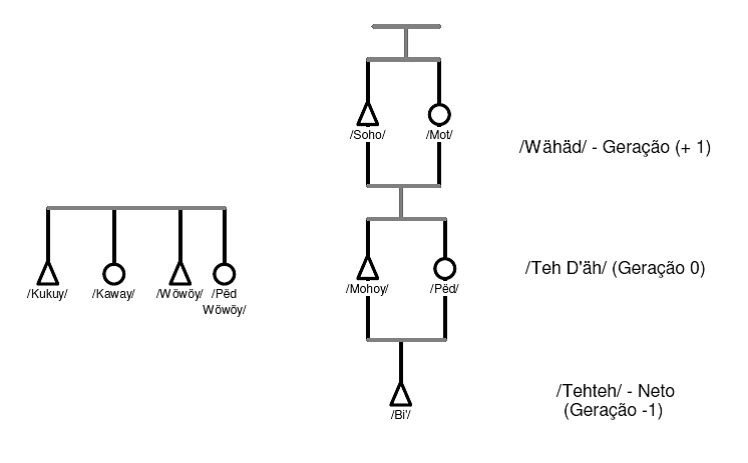
\includegraphics[width=\textwidth]{./img/023}
% \caption{Relações matrimoniais e fraternais de conjuntos de
% flautas do clã \textit{Sokw'ä̗t Noh K'öd Te̖͂h}}
% \end{figure}

Os nomes dos trompetes são todos nomes de animais como \textit{Moho̖y},
Veado, \textit{Kuku̗y}, Macaco"-da"-Noite, sendo que muitos deles
correspondem ao conjunto de nomes masculinos do clã \textit{Sokw'ä̗t}. Da mesma
forma, os nomes das flautas, cujo sentido remete a frutas como \textit{Pë̖d},
Cunuri, \textit{Mo̗t}, ou solos como \textit{Mu̖n}, Caatinga, compõem igualmente
o conjunto de nomes femininos do clã \textit{Sok'wä̗t}. Por fim, cada par de
dançarinos com suas flautas forma uma unidade geracional, havendo
instrumentos \textit{avós}, \textit{pais}, \textit{crianças} ou \textit{netos}, como é o
caso do flautim \textit{bi̖'}. De uma forma surpreendente, muitas das relações
sociais dos participantes do Dabucuri estabeleciam também a
sociabilidade dos instrumentos.

Como descreve Piedade, o conjunto de instrumentos tem sempre um trompete
como aerofone principal, o \textit{chefe}. Seu toque é repetido pelos demais
de acordo com as particularidades de articulação de cada instrumento
(técnica \emph{hocket}). Assim, nos pares, a fêmea repete o macho e
ambos repetem o \textit{chefe}. Ancestrais clânicos, os trompetes (machos)
podem apenas ser tocados por descendentes vistos como \textit{nɨ̖h ba̗bd'äh},
``nossos irmãos'', ou seja, agnatos reais ou classificatórios. Por outro
lado, as flautas (fêmeas) podem ser tocadas tanto pelos \textit{yo̖h d'äh},
``cunhados'', como pelos \textit{irmãos}. Os pares de dançarinos alternam"-se,
desse modo, entre duplas de agnatos ou duplas de afins, sempre tendo
como termo marcado o instrumento macho. As \textit{segundas flautas}, irmãs
ou esposas, constituem uma posição não marcada que pode ser ocupada de
forma a aludir a relações endogâmicas ou exogâmicas. Segundo Piedade que
analisou a Música de Jurupari dos Tukano,

\begin{quote}
Como na Música de Cariçu e de Japurutu, emprega"-se aqui uma técnica de
alternância em cada par de instrumentos, no entanto os papéis e as
regras são bastante diferentes. Novamente os papéis de chefe e
respondedor são associados a um instrumento macho e uma fêmea. Mas além
disso, os instrumentos miriá representam seres musicais da natureza, com
nomes de animais, cada um dotado de uma força espiritual específica. O
representante macho destes seres é o trompete, feito de paxiúba,
enquanto a fêmea é uma flauta, feita de jupatí. De fato, no simbolismo
Jurupari a questão do gênero (\emph{gender}) é uma temática central que
perpassa todos seus elementos. Os miriá"-põ'ra e a Música de Jurupari são
segredos dos homens.\footnote{1997, p.\,115.}
\end{quote}

De forma semelhante, no evento de Jurupari presenciado por mim, as
relações entre os pares de trompete e flauta delineiam"-se através de
diferenciações de gênero, de função musical (chefe, ou respondedor) e de
timbre que apontam também para um poder maior dos instrumentos
\textit{machos} com nomes de animais. Nos dois conjuntos representados em
esquema, é possível dizer que no grupo da direita a ênfase recai sobre
uma endogamia extrema, ao contrário do grupo de irmãos à esquerda. Os
diagramas podem ser lidos como modos de relação possíveis dos irmãos com
suas irmãs, quer os primeiros as tomem por esposas, negando assim a
aliança com grupos afins, quer aceitem considerá"-las apenas irmãs,
estabelecendo relações de afinidade com outros clãs.

Como descreve Reid, a estrutura social hup está baseada numa organização
clânica, havendo dois grupos de clãs hierarquicamente ranqueados e
correlacionados por afinidade (grupos exogâmicos). Cada clã é um grupo
de descendência patrilinear cujos membros são \textit{Te̖͂h däh}, os Filhos
de um mesmo ancestral fundador. Na \emph{performance} do Jurupari, uma
das formas de designar alguns dos trompetes é chama"-los de \textit{wähä̗d},
``anciões'', o que os vincula a uma geração (+ 1) da qual descendem os
instrumentos Filhos (0) e o pequeno flautim, um \textit{Te͂te͂h}, ``neto''
(-1). Com a dança e o toque, os instrumentos passam a ser ancestrais
fundadores dos clãs trazidos à vida pelo sopro dos descendentes. O autor
mostra ainda que a terminologia de parentesco distingue cinco gerações,
sendo duas acima e duas abaixo de ego. Assim, ao longo de sua vida, cada
indivíduo move"-se através de três gerações assumindo o lugar de filho,
de pai e de avô, de forma semelhante à diferenciação entre as flautas
Jurupari (1979, p.\,117).

%\begin{figure}
%\centering
%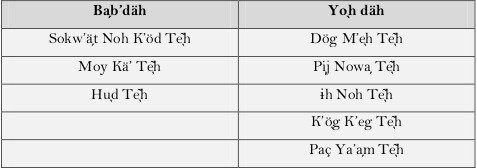
\includegraphics[width=\textwidth]{./img/q5}
%\caption{Quadro de grupos exogâmicos presentes em \textit{Ta̗t"-Dëh} divididos em
%/bab'däh/, ``irmãos'', e /yo̖h däh/, ``cunhados'', segundo a perspectiva
%do clã majoritário /Sokw'ä̗t Noh K'öd Te͂h/}
%\end{figure}

% Please add the following required packages to your document preamble:
% \usepackage{booktabs}
% Verificar tabela
% \begin{table}[]
% \centering
% \begin{tabular}{@{}ll@{}}
% \toprule
% \textbf{Ba̗b’däh} & \textbf{Yo̖h däh} \\ \midrule
% Sokw’ä̗t Noh K’öd Te̖͂h & Dög M’e̖h Te̖͂h \\
% Moy Kä’ Te̖͂h & Pi̖j Nowa̗ Te̖͂h \\
% Hu̖d Te̖͂h & ɨh Noh Te̖͂h \\
%  & K’ö̖g K’eg Te̖͂h \\
%  & Paç Ya’a̗m Te̖͂h \\ \bottomrule
% \end{tabular}
% \caption{Quadro de grupos exogâmicos presentes em \textit{Ta̗t"-Dëh} divididos em
% \textit{bab'däh}, ``irmãos'', e \textit{yo̖h däh}, ``cunhados'', segundo a perspectiva
% do clã majoritário \textit{Sokw'ä̗t Noh K'öd Te͂h}}
% \label{q7}
% \end{table}

Seguindo Reid, a divisão entre os clãs forma dois grandes grupos
exogâmicos não nominados que não geram um senso de pertencimento. Já os
aproximadamente 25 clãs nominados criam um forte senso de incorporação e
alteridade com outros clãs, levando seus membros a se perceberem num
plano geral como Hupd'äh. Cada clã relaciona"-se com o outro como irmão
maior (\textit{sät}) e irmão menor (\textit{yawa̗m}). A partir do sistema de
descendência patrilinear, observa"-se a prerrogativa do casamento entre
primos cruzados bilaterais reais. Com base nisso, as relações
matrimoniais entre instrumentos irmãos poderiam ser descritas como
casamentos incestuosos ou casamentos ``ruins'', \textit{pa̗y}. Entretanto, como
mostra Reid, são percentualmente raros os casamentos entre primos
cruzados bilaterais reais, sendo mais comuns aqueles entre primos
cruzados classificatórios de modo unilateral. A recorrência de número
considerável de casamentos entre membros de clãs agnatos ou com membros
do mesmo clã e a inexistência de sanções a tais uniões revelam a
importância dos casamentos com agnatos próximos.

Portanto, a ênfase em relações endo- ou exogâmicas entre os pares de
instrumentos situa, através da forma de interações da
\emph{performance}, as linhas que norteiam o sistema de parentesco hup
definindo a aliança matrimonial em termos de uma exogamia clânica de
grupos, mas tendo na endogamia entre clãs agnatos ou entre membros do
mesmo clã uma prática importante. A sequência de ações que se seguiu na
maloca após a saída das flautas foi especialmente interessante para
entender os papéis femininos e masculinos e as dimensões endo- e
exogâmicas nesse circuito de trocas.

\section{A dádiva do buriti}\label{a-duxe1diva-do-buriti}

No dia seguinte, quando as flautas já haviam deixado a maloca para
retornar a seu abrigo ribeirinho, mães, senhoras e moças dirigiram"-se à
palhoça com seus aturás. Começaram a recolher os frutos amontoados no
espaço central. Riam, conversavam, seguravam seus bebês no colo. As
crianças corriam para lá e para cá, desconhecendo o que havia se passado
durante a madrugada. Com os cestos plenos de frutos, elas foram deixando
a maloca e dirigindo"-se a suas casas. Logo retornaram carregando grandes
bacias de metal cheias de massa de tapioca para ser dada aos homens em
retribuição pela dádiva de buritis recebida. As bacias foram colocadas
no centro. Ocupavam agora o local onde antes se amontoara o buriti. De
modo interessante, os parceiros de troca do Dabucuri que presenciei não
eram parentes de outra aldeia, ou pessoas de outra etnia, mas, sim,
``homens'', \textit{tiyi̖' d'äh}, de um lado, que ofereciam os buritis da mata
às ``mulheres'', \textit{tã'ã̗y d'äh}, da comunidade. Como nas relações entre as
flautas, as relações de gênero mostravam"-se fundamentais para a
interação da troca de alimentos.

Postando"-se próxima à oferenda, Tereza iniciou uma fila de mulheres que
se estendeu até a Porta da Cabeceira, \textit{Dëh K'et Yoh Moyo̗}. Defronte
à professora, Mandu ficou em pé e deu início a uma fila de homens que se
esticou no sentido da Porta do Sol Nascente, \textit{Sa̗ka̗n Moyo̗}. Os
porta"-vozes iniciaram, então, as falas formais de agradecimento. Rindo e
meio sem jeito, Tereza voltou seu olhar para Mandu, mencionou o
sofrimento e os perigos enfrentados pelos homens para trazer e ofertar o
buriti. Em retribuição, as mulheres ofertavam a massa de tapioca com a
qual fariam beijus para alimentá"-los. Em nome dos homens, Mandu
agradeceu, louvando igualmente a bravura dos rapazes e o trabalho duro e
diário das mulheres na lida com a roça. Concluídos os pronunciamentos,
os homens recolheram as bacias oferecidas e levaram"-nas para casa. As
mulheres trouxeram suas panelas com caxiri e começaram a circular
oferecendo cuias aos homens já sentados. Comentando sobre os Dabucuri
realizados atualmente entre parceiros Tukano e Tariano na região de
Iauareté, Andrello afirma que:

\begin{quote}
O dabucuri estabelece, portanto, uma espiral de prestações e
contraprestações, pois para cancelar o débito criado é preciso um outro
dabucuri, no qual as posições irão se inverter. Apesar da plasticidade
que envolve o ritual --- atestada pelas novas situações que passam a
ocorrer hoje em dia ---, sua estrutura básica refere"-se essa justaposição
de identidades, cuja epítome é a relação entre dois grupos que trocam
mulheres, isto é, a relação entre cunhados. Tal relação é, precisamente,
a que se verifica entre os Tariano e Tukano.\footnote{2011, p.\,18.}
\end{quote}

No caso, as prestações e contraprestações no evento descrito colocam"-se
entre um grupo de homens e outro de mulheres, ambos os grupos justapondo
suas identidades de gênero ao mesmo tempo em que expressavam a
importância dos laços de afinidade clânica. Mas, para entender em que
medida a dádiva de buritis situa as relações de aliança entre os clãs de
\textit{Ta̗t"-Dëh}, é necessário detalhar um pouco melhor como se dá a preparação
e realização dos Dabucuris. Conversando com Américo, ele me explicou que
se pode realizar oferecimentos de diversos tipos de \textit{s'u̖gu̖t a̗g},
``frutas do mato'' como: ucuqui, buriti, açaí, \textit{mo̗t},\footnote{Tipo de cunuri.}
ingá \textit{po̗-min}, cucura do mato \textit{pɨ̖͂g}. Em suas palavras,

\begin{quote}
Quando cai ucuqui, vai ver no mato. Depois conversa com o pessoal: \textit{Eu
queria fazer Dabucuri para vocês}. O outro pergunta \textit{quantos dias dá
pra tirar?}. O que tá oferecendo diz se em três, quatro ou cinco.
\textit{Já! Eu quero}, responde o Joaquim, \textit{bora tirar}. Vão em grupo. O
outro fala: \textit{Vamos arrancar maniva pra fazer caxiri!}.\footnote{Caderno de
campo, abril de 2012.}
\end{quote}

Uma grande caça, a obtenção de muitos peixes ao tinguejar um igarapé ou
a maturação de uma enorme quantidade de frutos da mata são eventos que
motivam os parceiros de troca ao oferecimento. O arranjo envolve a
divisão dos papéis e a distribuição das tarefas para que a coleta, por
exemplo, leve à obtenção de um volume grande de frutas. Será considerado
o ``dono do Dabucuri'', \textit{pä̗' yo'o̖m i͂h}, aquele que \textit{ë̗yë̗p}, ``chamou a
ação'', ao perceber a maturação da fruta. É ele o \textit{kɨhsä̗t}, o
``primeiro'', que será seguido por seus parceiros de troca os \textit{hu͂y ha̗m
däh}, os ``acompanhantes'' ou os ``seguidores''. Como durante as
caminhadas em que o grupo de viajantes segue um \textit{kɨhsä̗t}, ``guia'' ou
``mentor'', o acordo de troca inicial define, de um lado, o \textit{kɨhsä̗t
ë̗yë̗p}, que será o dono a quem cabe coordenar os preparativos e produzir
uma grande quantidade de caxiri, e, de outro, os \textit{hu͂y ha̗m däh}, membros
de clãs afins ao do dono que devem organizar o trabalho dos rapazes para
que estes colham as frutas e as tragam para as imediações da aldeia.

Além da capacidade de observação, o \textit{dono chamador} deve certificar"-se
com a esposa da possibilidade de colheita de grande quantidade de
manivas para o preparo do caxiri que será oferecido aos dançarinos,
carregadores e demais presentes enquanto as flautas Jurupari forem
tocadas. A esposa do \textit{dono chamador} conta com a ajuda de suas filhas,
noras e sobrinhas para conseguir dar conta do preparo do volume exigido
pelo evento. O marido e seus filhos contribuem ajudando a carregar os
aturás, repletos de maniva, da roça até a casa. Por vezes, nas noites
que precedem as grandes festas de caxiri ou Dabucuri, é possível ouvir
as mulheres reunidas até tarde conversando e ralando a maniva,
cozinhando a manicuera ou esfregando a massa de caxiri no fundo das
``canoas de caxiri'', \textit{hu̗ptök hoh"-tëg}.

Quando o caxiri começa a ficar pronto, o \textit{dono chamador} benze ou pede
que seu pai sopre a canoa para acentuar a força e a fermentação da
bebida. Além da ação xamânica, o dono pode misturar caldo de cana ao
caxiri para acelerar a fermentação. No final da tarde, ele espera a
todos com uma grande canoa de caxiri plena de bebida. Ao longe,
começa"-se a ouvir o som das flautas Jurupari soar. Antes de retirar o
Jurupari do igarapé, é preciso que os dançarinos se banhem e bebam
algumas cuias de \textit{bi'i̖d hu̗ptök}, ``caxiri benzido'', na casa do dono
para intensificarem a energia quente de seus corpos. Com a aproximação
dos instrumentos, as panelas de caxiri começam a \textit{ferver}
intensamente. Nas palavras de Américo:

\begin{quote}
O caxiri vai fervendo conforme vai chegando o Jurupari. O chefe do
caxiri está chamando. Ele fala: ``Já chega, vocês sofreram muito no
mato, muito perigo. Agora vocês vão viver bem. Ele oferece duas cuias do
caxiri benzido. Todos bebem e ficam bêbados rápido. O dono fala: \textit{Hu̖͂t
döh tu̗u̗y. Hup he̖me̖y s'u̖gu̖t, tɨ͂hɨ̗͂y ni̗i̗, Bisi̗w ni̗i̗, Döh Ã̗y ni̗i̗. Hu̗ptök
ne̗ne̗n. K'o̗po̗p}, ``Vocês querem tabaco. Vocês sofreram na mata onde há
muita jararaca. Passaram pelos perigosos domínios do \textit{Bisi̗w}, da \textit{Döh
Ã̗y}. O caxiri já vem. Eu ofereço para que vocês se satisfaçam''.\footnote{Caderno de campo, abril de 2012.}
\end{quote}

Novamente, o dono \textit{chama} seus seguidores através do caxiri fervente.
Ele recebe aqueles que se arriscaram nos dias anteriores para colher e
carregar os cestos com frutos da mata. Passaram pelos territórios de
seres como \textit{Bisi̗w} e \textit{Döh Ã̗y}, muitas vezes retirando os frutos de áreas
consideradas como roças desses perigosos seres. Em sua fala, o dono
acolhe aqueles que sofreram e demonstraram sua valentia ao vencer tantos
perigos. Como retribuição, oferece a bebida extremamente embriagante e o
tabaco. Por volta das três da madrugada, quando todos já beberam
bastante e muitas danças foram realizadas com as flautas, o chefe fala:
\textit{A̗g ã̗h d'ö̗' ne̗n tëg}, ``Vou juntar a fruta'', e começa a abrir e a
despejar os cestos no centro da maloca.

Desse modo, o bom desempenho do papel de \textit{dono chamador} depende da
relação entre o dono com um grupo de mulheres composto por sua esposa,
suas filhas e sobrinhas (\textsc{bd}) que trabalharão intensamente para que ele
consiga realizar sua oferta de caxiri. Por outro lado, seus parceiros de
troca dependem do esforço e da capacidade de seus filhos e sobrinhos na
colheita e no carregamento de frutos. O \textit{oferecimento de caxiri} e o
\textit{derramamento de buritis} podem ser vistos como ações de troca entre
grupos afins que se tornam viáveis apenas graças à relação dos
\textit{acompanhantes} com seus descendentes agnatos, e do \textit{dono chamador}
com sua esposa e filhas. De um lado, a colheita de frutos é garantida
pelo respeito dos rapazes (-1) por seus \textit{sät däh}, ``irmãos maiores'',
agnatos da geração ascendente (0). Por outro lado, a complementaridade
das atividades produtivas no interior do grupo doméstico (\textit{kaka}) entre
o dono da casa e sua esposa e filhas é o que assegura o preparo e
oferecimento do caxiri.

A descrição de Américo ajuda a entender alguns dos papéis dos
participantes do Dabucuri que presenciei em 2011. O dono do caxiri era
Pedro Paulo, filho mais velho de Miguel, homem de referência do clã afim
\textit{Dög M'e̖h Te̖͂h}. Era ele quem servia as cuias de caxiri aos carregadores
cansados e foi também quem derramou os buritis no centro da maloca. A
cerimônia das flautas pode ser vista como o oferecimento de caxiri por
esse dono aos carregadores, rapazes membros do clã \textit{Sokw'ä̗t Noh K'öd
Te̖͂h}. Durante a dança das flautas eram os filhos e netos desse clã que
estavam sendo iniciados e, por isso, os instrumentos tocados pertenciam
a esse clã.

Eram eles que levavam surras com o ramo de ingá nas pernas, braços e
antebraços e foram também os que deixaram a maloca antes da saída das
flautas. Essas ações permitem vê"-los como neófitos participando de um
contínuo de ações ritualizadas. As flautas do clã \textit{Sokw'ä̗t} foram
tocadas para transformar esses rapazes em homens. O esforço físico para
o carregamento do peso, o afastamento da comunidade para áreas perigosas
na mata, o percurso pelas trilhas e as surras com ramos de ingá
delineiam as condensações rituais que vão aos poucos transformando os
rapazes em homens.

É possível ver agora a fila formada pelas mulheres como uma sequência
feminina de membros do clã majoritário. Sandra,\footnote{Sandra (\textit{Mo̗t},
  nasc. 1987).} esposa de Pedro Paulo, é membro do clã \textit{Sokwä̗t Noh K'öd
Te̖͂h}, assim como Tereza, esposa de Elias e Angelina, esposa de Mandu. A
dádiva às mulheres era também uma celebração das alianças estabelecidas
com os donos locais a partir dos casamentos com irmãs e filhas
\textit{Sokw'ä̗t}. A fila masculina era composta por aqueles que se fixaram em
\textit{Ta̗t"-Dëh} após se casarem com as irmãs, filhas ou netas dos \textit{Sokw'ä̗t}. A
recorrência de uniões que levaram os homens a estabelecer a moradia da
família num local próximo de onde vivem os cunhados e sogros ressalta a
importância das mulheres \textit{Sokw'ä̗t} para a consolidação de uma tendência
à uxorilocalidade dos membros de clãs \textit{de fora} (80\% dos casados) e
uma virilocalidade dos membros do clã majoritário (87\% dos casados).

As falas de Mandu no diálogo formal com Tereza são palavras proferidas
por um ancião do grupo de afins moradores de \textit{Ta̗t"-Dëh}. Ele é, ao mesmo
tempo, um ``tio classificatório'', \textit{pã̗ç} de Pedro Paulo. Sua
interlocutora é a filha do falecido Joanico, ancestral de referência de
uma das linhagens dos \textit{Sokw'ä̗t Noh K'öd Te̖͂h}. Assim, através do
Dabucuri, homens membros de clãs afins ofertavam buritis às mulheres
\textit{Sokw'ä̗t}, muitas vezes suas esposas e cunhadas. Pela via dessa mediação
feminina, a reciprocidade de gêneros recolocava a dádiva entre afins.
Num próximo encontro de Dabucuri seriam os donos \textit{Sokw'ä̗t} que deveriam
retribuir as ofertas, quer às mulheres, quer a seus cunhados.

% Verificar tabela
% \begin{figure}
% \centering
% 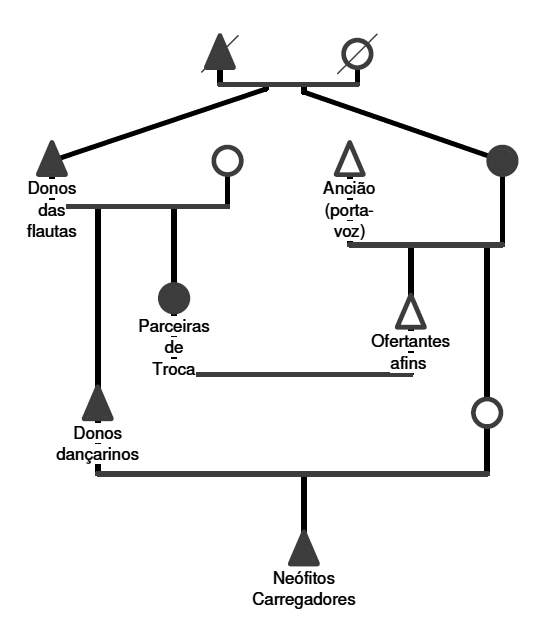
\includegraphics[width=\textwidth]{./img/024}
% \caption{Papéis rituais: clã \textit{Sokw'ä̗t Noh K'öd Te̖͂h} e clã
% afim \textit{Dög M'e̖h Te̖͂h}}
% \end{figure}

Tomando como referência a posição ocupada pelos neófitos, é possível
observar que o oferecimento de buritis e a contrapartida em massa de
tapioca eram realizados por tios maternos (\textsc{mb}) e tias paternas (\textsc{fz})
reais ou classificatórios, dependendo do neófito em questão. Através da
dádiva do buriti, o gesto de oferecimento e as falas evocavam as duas
relações de aliança consideradas ideais para o casamento, ou seja, a
união entre primos cruzados bilaterais. Se uma das ações importantes do
Dabucuri vem a ser transformar os rapazes em homens capazes de realizar
atividades árduas, deslocar"-se pelos caminhos e enfrentar a ameaça de
seres como \textit{Bisi̗w} e \textit{Döh Ã̗y}, tais esforços os tornam capazes de tomar
mulheres como esposas e exercer seus papéis de maridos, obtendo
alimentos, ensinando os filhos e convivendo com seus afins.

Tendo as mulheres \textit{Sokw'ä̗t} ocupado o papel de parceiras de troca, o
evento que presenciei foi fundamental para uma observação do Dabucuri
como uma forma de interação marcada por agências masculinas e femininas
que promovem interessantes condensações rituais em torno das relações de
aliança matrimonial e de descendência clânica. As flautas ancestrais
(fêmeas) constituem uma posição aberta à composição de duplas de
dançarinos entre afins. Na dança do Jurupari, as flautas (fêmeas)
sopradas pelos cunhados revelam a participação desejada desses afins na
iniciação dos rapazes para que, futuramente, novas alianças se
consolidem entre os diferentes clãs no interior do grupo local.

Distantes da maloca enquanto as flautas eram tocadas, as mulheres
exerceram um papel fundamental durante a cerimônia de troca. Tias
paternas (\textsc{fz}) elas não só geram filhas que poderão ser as esposas dos
neófitos, como também são atoras fundamentais nos movimentos uxorilocais
que configuram boa parte dos matrimônios em \textit{Ta̗t"-Dëh}. Essa capacidade
de atração contribui para fixarem"-se sogros e cunhados potenciais,
criando um ambiente favorável aos casamentos dos neófitos. Além disso, o
oferecimento de caxiri do \textit{dono chamador} depende do trabalho das
mulheres do grupo doméstico. É a complementaridade entre as atividades
produtivas masculinas e femininas do grupo doméstico que garante, nesse
nível, a produção da quantidade necessária de caxiri. São também as
mulheres que garantem as alianças matrimoniais das quais depende a
descendência clânica.

Retomando a dança das flautas, é possível dizer que, tocando as flautas
(fêmeas) e oferecendo o caxiri, uma bebida produzida pelas mulheres, os
afins ocupam uma posição feminina, ao mesmo tempo em que exercem o papel
de anfitriões. Ao contrário, tocando os trompetes (machos) e oferecendo
os frutos adquiridos pelo trabalho masculino, os agnatos se postam como
convidados situados numa posição masculina. Da dança das flautas para a
troca de alimentos, as posições se invertem, passando as mulheres
\textit{Sokw'ä̗t} a ocupar um papel feminino, ofertando, como anfitriãs, um
produto de seus trabalhos. Já os homens de clãs afins passam a ser os
doadores das frutas colhidas por seus primos e sobrinhos cruzados (\textsc{zs}),
ocupando, assim, um lugar masculino de convidados no Dabucuri. Ao
descrever as múltiplas formas de percepção da maloca tukano durante os
Dabucuris e cerimônias de Jurupari, Hugh"-Jones refere"-se à maloca como
sendo uma Casa Andrógena.

Entendo que a sequência de ações ritualizadas que presenciei se
estabelecia através de pares \emph{masculino e feminino}, \emph{sênior e
júnior}, \emph{marido e esposa}, \emph{irmão e irmã}, \emph{irmão maior
e menor} que situavam relações de consanguinidade e afinidade por meio
de modos de interação marcados ora pela simetria, ora pela assimetria. A
relação dos mentores, senhores e homens adultos, com os rapazes
baseia"-se na alternância das gerações num grupo de descendência que faz
com que os primeiros guiem os mais jovens pelos caminhos, curem"-nos e
protejam"-nos com o xamanismo, contem mitos e histórias dos antigos,
criem as condições para a transformação do guerreiro. Ao mesmo tempo, os
neófitos arriscam"-se na mata, carregam cestos pesadíssimos, aceitam os
açoites e obedecem a seus seniores. Já a reciprocidade entre afins cria
séries de posições masculinas e femininas pelas flautas e trompetes,
pelos alinhamentos de gênero durante o oferecimento ou pelo preparo e
oferecimento do caxiri para situar consanguíneos e afins nas posições de
doadores e receptores no circuito das dádivas. Seguindo Houseman e
Severi (2009, p.\,163), parece que ``é a forma do campo relacional no
qual os protagonistas são engajados que orienta o estabelecimento de um
contexto próprio ao comportamento ritual''.

A circulação dos casais de flautas e dos pares de dançarinos
(afins, ou agnatos) fazia com que os participantes se vissem através dos
olhos dos outros nas mudanças de perspectiva geradas pela dádiva de
buriti e pela oferta de caxiri. Desse modo, entendo que os pares
\emph{cônjuges/\,irmãos} da dança e os grupos de \emph{gênero/\,afinidade}
dos parceiros de troca mostram que os princípios de aliança matrimonial
são elaborados ritualmente tanto na cerimônia de troca de alimentos, que
enfatiza a celebração dos laços entre afins, como na dança do Jurupari,
cuja ênfase recai sobre a descendência. A partir de elementos ora
semelhantes, ora diferentes dos Tukano, a androgenia da maloca hup cria
um vasto campo de interações através do qual pessoas diferentes ocupam
as posições de doador e receptor, e situam formas múltiplas de
reciprocidade.

%\section{Cuias de coca}\label{cuias-de-coca}

\section{Flautas e domínios}\label{flautas-e-domuxednios}

Numa roda de coca no ano seguinte, conversando com os senhores hup sobre
a cerimônia de Jurupari que presenciei, Ponciano contou sobre os perigos
que os ancestrais enfrentaram para trazer as flautas Jurupari do Lago de
Leite dentro da Cobra"-Canoa. Todas as vezes que as flautas são tocadas e
trazidas para a maloca, é preciso que os participantes enfrentem
novamente os perigos da interação com o \textit{Bisi̗w}, as Gentes"-Cobra,
Gentes"-Árvore e demais seres que possam agir contra as pessoas hup.
Caminhar com as flautas e dançar na maloca são ações através das quais
os participantes do ritual refazem os percursos e deslocamentos dos
ancestrais ao trazerem as flautas e ao tocarem"-nas pela primeira vez. Ao
mesmo tempo, os conjuntos principais de instrumentos pertencem aos donos
locais, senhores como Ponciano e Firmino, a quem são atribuídos
territórios, agrupamentos residenciais e rodas de coca.


\begin{quote}\index{26@\textsc{m}17\quad Viagem com as flautas}
\mito{17}{viagem com as flautas}

Os Ancestrais, \textit{Hib'a̗h te̖͂h d'äh}, apareceram em Ipanoré. Daí, foram
dentro da Cobra"-Canoa para o Lago de Leite para receber suas coisas.
Receberam coca, tabaco, as histórias, a zarabatana, o arco e a flecha, o
pilão de coca, tudo. Todas as etnias receberam e depois vieram na
Cobra"-Canoa. Foram para o Papuri primeiro. Lá há o \textit{hib'a̗h kä̗d},
``banco de nascimento''. Em seguida, foram para \textit{Dëh Pohot},
Caruru"-Cachoeira. Dali, foram para \textit{S'ɨ̗g"-Mo̖y"-Paç}, Serra da
Iniciação. Foi lá que \textit{K'e̖g"-Te͂h} deu as flautas sagradas.

Foram então para \textit{To̗͂h"-Paç}, Serra dos Porcos. Lá em \textit{Tõ̗h} há um
cemitério dos \textit{Sokw'a̗t Noh K'öd Te̖͂h}. Essa Serra da Iniciação é na
cabeceira do \textit{K'a̗j"-Dëh}, Igarapé"-Cutivaia. Fui lá com meu pai. Há um
caminho, mas está muito ruim. Em \textit{Su̗g"-Dëh}, Igarapé"-Beija"-Flor, há
os ancestrais dos \textit{Paç Ya'a̗m Te̖͂h}. Já os ancestrais dos \textit{Dög M'e̖h Te̖͂h}
ficam na cabeceira de \textit{Ta̗t"-Dëh}. As flautas sagradas foram dadas aos
homens na Serra da Iniciação.

As flautas vieram do corpo queimado do \textit{Bisi̗w}. Ele comeu as crianças
pelo ânus e depois foi queimado pelos pais. De seu corpo fizeram"-se as
flautas. Seu \textit{hã̗wäg} saiu e foi para a \textit{Paç"-Mo̖y}, Casa"-de"-Pedra.

Houve um tempo em que eram as mulheres que tinham as flautas. Os homens
não sabiam fazer roça. Elas não sabiam tocar os \textit{Döhö däh},
Jurupari. Não tinham vagina nem menstruavam. Por causa da posse das
flautas Jurupari elas ficaram doentes e morreram, todas elas.

Tocar as flautas lava as frutas e a carne. \textit{Bisi̗w} não aparece, mas fica
ouvindo. As mulheres, quando roubaram as flautas, ficaram sem saber ter
filhos. Acabaram morrendo. Hoje, as mulheres têm muito medo. As flautas
ficam no igarapé para as mulheres não verem. A cerimônia faz os jovens
transformarem"-se em guerreiros. Se as mulheres virem, morrem todas.\footnote{Ponciano, 26 de fevereiro de 2012.}
\end{quote}

\index{26@\textsc{m}17\quad Viagem com as flautas}
\index{ag@\textsc{b}6\quad \textit{Te͂h Bi'i̖d}\break Benzimento do filho}
Em \textsc{m17}, a navegação pelo Rio de Leite na Cobra"-Canoa permite
aos ancestrais receber os alimentos primordiais, coca e tabaco, as armas
de caça, arco e flecha e zarabatana, o pilão para o preparo da coca e as
histórias.\footnote{As inúmeras referências presentes nas narrativas,
  encantamentos (\textsc{b6}) e cosmografia à viagem na Cobra"-Canoa após a
  emergência pelos buracos do surgimento em Ipanoré, designada pelos
  Hupd'äh como \textit{Hib'ah Huh}, Cachoeira do Nascimento, tornam
  necessária a revisão da afirmação de Reid (1979) e Athias (2010) de
  que a jornada na Cobra ancestral não estaria presente na mitologia
  hup.} No retorno à planície do Uaupés, os ancestrais sentam"-se para
conversar nos \textit{bancos de nascimento} às margens do rio Papuri, para
comer coca, fumar e \textit{saber como iriam habitar aquelas terras}
(\textsc{m13}). Após essa roda de coca primordial, os viajantes seguem
caminhando até a Serra da Iniciação, onde recebem as flautas Jurupari
como uma segunda dádiva de \textit{K'e̖g"-Te͂h}.
\index{22@\textsc{m}13\quad A dádiva da coca e do tabaco}

Ocorre, então, uma separação dos ancestrais que levam suas flautas e
passam a habitar regiões distintas. Ponciano menciona um cemitério do
clã \textit{Sokw'ä̗t Noh K'öd Te̖͂h} na região da Serra dos Porcos para referir"-se
ao primeiro assentamento de seu clã. Fala também dos territórios
originários de dois importantes clãs afins aos \textit{Sokw'ä̗t Noh K'öd Te̖͂h},
os \textit{Paç Ya'a̗m Te̖͂h}, que foram habitar as margens do Igarapé"-Beija"-Flor,
e os \textit{Dög M'e̖h Te̖͂h}, que seguiram para a cabeceira do Igarapé"-Taracuá.
Os antepassados desses clãs estão enterrados nesses primeiros
assentamentos, de onde partem seus caminhos, trilhas que atualmente se
encontram cerradas. Depois de descerem da Serra da Iniciação, caminhando
com as flautas sagradas, os diversos grupo constituíram territórios
originários, aos quais os Hupd'äh se referem como \textit{nɨ̖h s'a̗h}, ``nossa
terra''. Como descreve Athias, cada clã utiliza uma área comum
delimitada, no interior da qual perambulam e desenvolvem atividades
produtivas.

\begin{quote}
Para os Hupd'äh, nîh s'ah representa o espaço, o lugar, o território que
eles podem perambular, andar, caçar, neste caso, no interior da
floresta, os fazem parte deste mundo, mas habitado, com donos. A ideia
de fronteira existe, é como se eles estivessem ligados a esta terra
podendo usufruir de todo espaço necessário na floresta, no interior, o
que tenho chamado de área interfluvial. Cada clã hupd'äh utiliza uma
área comum e neste espaço encontram"-se os locais onde K'ég"-teh esteve
durante a criação do mundo.\footnote{2010, p.\,61.}
\end{quote}

\index{26@\textsc{m}17\quad Viagem com as flautas}
De modo interessante, os eventos narrados por Ponciano em \textsc{m17}
iluminam muitos dos acontecimentos que levaram à formação da comunidade
de \textit{Ta̗t"-Dëh}. Os ancestrais das famílias \textit{Sokw'ä̗t}, que hoje habitam
esse grande assentamento, nasceram e passaram suas infâncias numa Morada
Antiga, nas imediações da Serra Grande chamada \textit{B'o̖t"-Pe̗m"-Dëh Mo̖y"-Höd}.
Dos nove filhos que o avô (\textsc{ff}) de Ponciano teve, sete eram homens e
alguns deles deram origem a novas aldeias, caminhos e linhagens.
Referindo"-se a seus antepassados, Ponciano disse que seus tios paternos
brigavam muito nas festas de caxiri e, por isso, mudavam"-se e
constituíam novos assentamentos. Como mostra Pozzobon ao discutir a
mobilidade espacial dos povos Maku, as brigas são um dos fatores de
fissão dos grupos locais que leva um ou mais grupos domésticos a se
mudarem para se agregar a outro assentamento ou formar uma nova aldeia.

Esse foi o caso de Severiano, um \textit{sät}, ``irmão maior'', do
\emph{sibling}, que, após seu casamento e alguns desentendimentos,
constituiu uma morada chamada \textit{Hëhë Po̗ Mo̖y Höd}. Já Antônio, um dos mais
velhos, foi habitar a região de \textit{B'ö̖'"-Paç}. A formação do novo
assentamento envolvia a posse de conjuntos de flautas Jurupari por esses
que se tornaram donos de suas comunidades. Com o tempo, famílias de clãs
afins passaram a co"-habitar a morada desses senhores, devido ao
casamento de um(a) filho(a), pelo \emph{status} hierárquico desses
homens \textit{Sokw'ä̗t}, e pelas relações de troca mantidas por esses donos com
índios tukano ou comerciantes. A importância do processo de agregação de
famílias afins é descrita por Pozzobon como fundamental para a
composição cognática dos assentamentos, o que contribui para a
estabilidade e continuidade no tempo.

Entretanto, antes das primeiras visitas dos padres, esses ancestrais
\textit{Sokw'ä̗t} iniciaram conjuntamente um processo de constituição de
assentamentos.\footnote{Athias comenta que após muitas tentativas
  frustradas de evangelizar os Hupd'äh, nos anos de 1970, os
  missionários incitaram os Tukano a procurar famílias hup para
  catequizá"-las (2010, p.\,82). É possível ainda hoje encontrar
  indivíduos Tukano habitando assentamentos hup e desempenhando o papel
  de catequistas. Em \textit{Ta̗t"-Dëh}, esse é o caso do senhor Rosalino,
  catequista que se tornou cunhado do dono Firmino após casar"-se com sua
  irmã.} As novas moradas fixaram"-se em locais mais distantes das
cabeceiras e de acesso mais fácil aos comerciantes e índios tukano.
Durante a caminhada para a Serra Grande, passamos pelas Moradas"-Antigas
\textit{Pëd"-Dë̖h Mo̖y"-Höd}, onde Antônio voltou a habitar com seus irmãos
Francisco e Severiano. Segurando um pedaço de garrafa quebrada, Samuel
contou"-me que eram os restos da cachaça dos antigos, obtida em troca da
extração de látex, cipós e piaçava. Juntos, esses importantes donos
trouxeram seus conjuntos de flautas e passaram a realizar cerimônias de
Dabucuri constantemente, estabelecendo laços de reciprocidade
permanentes com as moradas de seus demais irmãos, espalhadas pela
região. Nosso percurso para a Serra Grande permitiu observar como os
assentamentos anteriores a \textit{Ta̗t"-Dëh} já vinham reaproximando os membros
desse \emph{sibling} que traziam consigo as famílias afins com as quais
coabitavam. Tomando como referência os dados de Pozzobon, esse movimento
de reaproximação do \emph{sibling} de mesmo sexo segue um padrão de
acordo com o qual os assentamentos hup procuram ``manter mais coeso o
grupo de \emph{siblings} de mesmo sexo, apesar de agregar afins''.

O aumento populacional vai se dando de modo progressivo e,
paralelamente, ocorre uma intensificação dos Dabucuri, que passam a ser
realizados tanto no interior desse grupo local, quanto externamente, com
aldeias do Igarapé"-Japú e com os Tukano do Tiquié. Nesse sentido, as
tentativas de \textit{atração} e composição de um povoado"-missão dos
salesianos articulam"-se de modo complexo a esse processo iniciado
anteriormente pelo \emph{sibling} \textit{Sokw'ä̗t}. Devido à presença
missionária, as cerimônias das flautas tornam"-se secretas aos brancos,
mas não menos constantes. Reid descreve a tendência de composição de
base agnática dos grupos locais hup com a agregação de famílias afins da
seguinte maneira:

\begin{quote}
Embora os Hupdʉ também empreguem esse princípio de aglutinação através
dos \emph{siblings} por gênero, o uso da aglutinação através dos
\emph{siblings} masculinos ocorre com maior frequência entre eles.
Consequentemente, a composição dos grupos locais Hupdʉ tende a ser menos
de base agnática do que entre os Bara"-Maku.\footnote{1979, p.\,127.}
\end{quote}

Desse modo, a formação do povoado"-missão de \textit{Ta̗t"-Dëh}, na década de
1970, reuniu membros de referência do clã \textit{Sokw'ä̗t Noh K'öd Te̖͂h} que
habitavam várias partes da região interfluvial dos igarapés \textit{K'a̗j"-Dëh} e
\textit{Pi̖j"-Dëh}. Atualmente, a comunidade é constituída por vinte e seis
``casas'', \textit{mo̖y}, concentradas às margens do Igarapé"-Taracuá. A
população da aldeia é de 202 indivíduos. Está dividida em trinta e oito
\textit{kaka}, ``grupos de fogo'', unidades familiares mínimas formadas
geralmente por um casal, seus filhos e alguns agregados. As moradas
abrigam desde um único grupo de fogo, um casal de união recente, até
famílias extensas, compostas por vários grupos de fogo. Como mencionado,
os senhores e senhoras hup habitam as moradas de um de seus filhos
casados. O dono de uma casa é geralmente um \textit{pu̗b i͂h}, ``homem adulto'',
casado e com filhos.

Como mencionado anteriormente, o senhor Henrique morava com sua família
nas cercanias da Serra da Cutivaia. Ao mudar"-se para a nova aldeia,
construiu sua casa próxima a uma trilha que o levava até o sítio de sua
antiga morada. Ao longo desse percurso, abriu roças com seus filhos, e
não deixou de pescar no \textit{K'a̗j"-Dëh} e caçar na serra. Trouxe consigo um
par de flautas (\textit{B'öh} e \textit{Wöwö̗y}) para tocar nos Dabucuris.
Acompanharam"-no os pais do senhor Miguel, parentes afins com quem esse
dono coabitava.\footnote{O pai de Miguel, sr. Antônio Oliveira, pertencia
  à etnia Dâw. Após fugir das investidas violentas de Manduca contra seu
  povo, ele foi acolhido pela família de Henrique e casou"-se com uma de
  suas primas paralelas do clã \textit{Hu̖d Te͂h} da região do Cabari"-Igarapé.
  Seus filhos são considerados Hupd'äh membros do clã \textit{Dög M'e̖h Te͂h}.
  Miguel e seus irmãos casaram"-se com mulheres \textit{Sokw'ät} tornando"-se
  importantes afins dos donos locais.} Henrique e seus filhos
tornaram"-se os donos de todo o território das imediações desse \textit{K'a̗j"-Paç
Ti̖w}, Caminho da Serra da Cutivaia. Até hoje, qualquer pessoa que
deseje abrir uma roça nessas terras, pescar nos igarapés, ou caçar deve
pedir permissão aos filhos de Henrique.

Numa festa de caxiri, Samuel revelou que as flautas \textit{Soho̗} e \textit{Mo̗t}
pertencem a seu pai, Ponciano, estendendo"-se a posse a ele e a seus
irmãos. São flautas médias que acompanharam as mudanças de Gustavo,
bisavô de Samuel (\textsc{fff}) e pai de Henrique (\textsc{f}). A flauta \textit{Soho̗} é
considerada a \textit{nu̗h}, ``cabeça'', a primeira numa hierarquia que
estabelece também seu grau de importância. \textit{Yo'o̗m i͂h}, ``dono'' de
\textit{Ta̗t"-Dëh}, Ponciano detém igualmente esse instrumento considerado o
\textit{Hib'a̗h Te͂h Döhö Pu̗b i͂h}, o Poderoso Ancestral Jurupari. Como no
caso da família de Henrique, o caminho que se abre de \textit{Ta̗t"-Dëh} e leva
até \textit{B'ö̖'"-Paç}, Serra do Tucunaré constitui o vasto território onde
Ponciano, seus irmãos e filhos abrem suas roças, pescam e caçam.%\footnote{Ver diagrama anexo -- Anexo 2.}

% Verificar tabela.
% \begin{figure}
% \centering
% 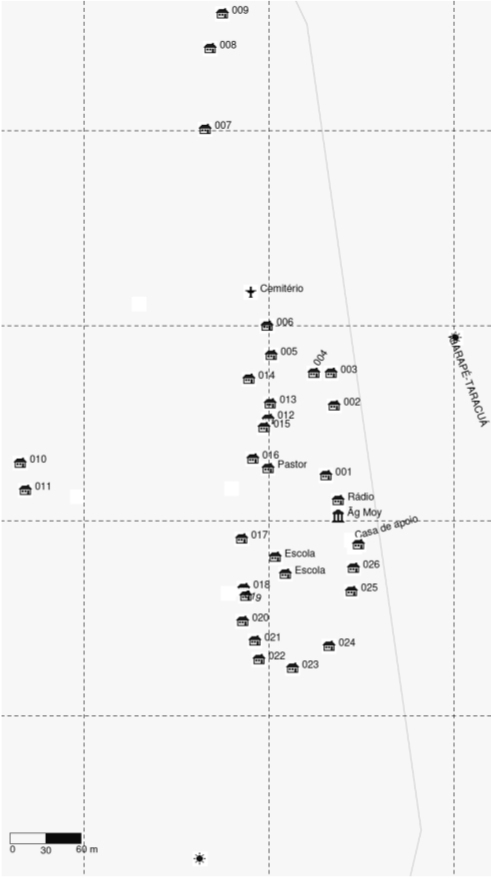
\includegraphics[width=\textwidth]{./img/025}
% \caption{Distribuição das casas de \textit{Ta̗t"-Dëh}}
% \end{figure}

Por ocasião da fundação de \textit{Ta̗t"-Dëh}, a reunião de muitos membros do
\emph{sibling} \textit{Sokw'ä̗t}, como Antônio, Francisco, Henrique, Joanico,
Paulino, fez com que conjuntos de flautas Jurupari, antes dispersos,
fossem concentrados e enterrados no Igarapé"-Vermelho. A coabitação
gravitava em torno da pessoa de Antônio, um irmã maior do grupo, que,
além de promover uma vida ritual intensa, atuou habilmente com sua
esposa Dabina para consolidar as relações com os missionários, os Tukano
e os comerciantes. Fabricados ou trazidos das antigas comunidades, os
Jurupari possibilitavam a iniciação de rapazes de diversos clãs e
linhagens.

Referindo"-se ao poder que seu avô passou a ter, Samuel contou sobre uma
batalha que seus antepassados tiveram com um grupo desana da região.
Após vencer o confronto, Antônio apoderou"-se da gigantesca flauta \textit{Bɨh
Kawah} dos inimigos. No evento que presenciei, esse instrumento foi
tocado pelos netos desse patriarca. Certa vez, Ponciano descreveu o
timbre inigualável desse Jurupari, \textit{tuhu̗p hõ̗h}, ``um som maravilhoso'',
exclamava o ancião a sorrir. Sempre que ouvem a \textit{Bɨh Kawah}, os filhos e
netos lembram"-se da valentia e da força desse antigo hup, um verdadeiro
\textit{u͂h me̗h i͂h}, ``guerreiro''.

Hoje, muitos dos descendentes de Antônio habitam a comunidade de
\textit{Ta̗t"-Dëh}. Quando os membros desse \emph{sibling} já estavam assentados
com as famílias afins que os acompanharam, outras famílias hup de clãs
afins ou agnatos começaram a visitar a nova comunidade por ocasião das
festas de caxiri ou Dabucuri. Algumas delas fizeram pedidos formais ao
dono para que pudessem se mudar para lá. Os afins obtiveram concessões
de uso de algumas áreas dos territórios de famílias \textit{Sokw'ä̗t} para abrir
roças ou pescar, condicionadas ao respeito dos limites estabelecidos
pelos donos. Seus territórios originários foram deixados em regiões
distantes. Sem possuir seus próprios caminhos, transitam pelos
territórios de seus ``cunhados'', \textit{yo̖h}, e de seus ``sogros'', \textit{k'o̗t}.
``Aqueles que são de outras terras'', \textit{sã̗p s'a̗h d'u̗u̗y d'äh}, são
considerados \textit{hu͂y ha̗m d'äh}, ``acompanhantes'' ou ``seguidores'',
aqueles que auxiliam seus donos na abertura ou capina de roças, na
extração de palhas de caranã para a cobertura dos telhados, na
realização de benzimentos para filhos e netos, e no papel de apanhadores
nas rodas de coca. A coabitação exigiu que as flautas desses outros clãs
fossem trazidas ou fabricadas para possibilitar a iniciação dos rapazes
afins. O domínio territorial e as alianças matrimoniais fazem com que os
donos ocupem continuamente a posição de \textit{kɨhsä̗t ë̗yë̗p}, ``donos
chamadores'', que são seguidos pelos \textit{acompanhantes}, seus afins reais
ou classificatórios.

Os motivos para a fixação desses grupos décadas atrás vão desde a busca
pela escola e capela inauguradas pelos salesianos, até a boa qualidade
dos solos para o plantio e a oportunidade de acesso a mercadorias
trocadas com os Tukano, cuja aldeia de beira"-rio dista algumas horas de
caminhada. Algo que sempre é mencionado pelos senhores hup quando
explicam o porquê da vinda de seus pais a \textit{Ta̗t"-Dëh} vem a ser a fama de
aldeia pacífica, com poucas brigas, que o assentamento possuía já
naquela época. A presença de muitos homens de alto ranque do importante
clã \textit{Sokw'ä̗t Noh K'öd Te̖͂h}, a realização frequente de Dabucuri e
cerimônias de iniciação com as flautas Jurupari e a atuação de poderosos
xamãs tornavam essa \textit{nova comunidade} uma morada especialmente
interessante para muitos dos antepassados. Seguindo a reflexão de Reid
sobre a mobilidade de grupos domésticos e indivíduos (\emph{short term
mobility}) é possível dizer que a busca por re"-expressar relações
sociais de um modo espacial norteou essa \emph{fluidez},\footnote{Reid
  (1979, p.\,123) entende que a mobilidade dos grupos domésticos
  baseia"-se num princípio de fluidez estrutural que leva o grupo local a
  ter uma grande capacidade de agregar unidades familiares ou clânicas
  ou fissionar"-se. Em suas palavras: ``A necessidade da estrutura social
  Hupdʉ de ser capaz de acomodar tal fluidez social no longo prazo
  advém, ao menos em parte, da natureza muito volátil do grupo local''.}
levando à fissão e agregação de diversos grupos em vários assentamentos
até a formação da aldeia de \textit{Ta̗t"-Dëh}.

Como mencionado, as casas do grande assentamento agrupam"-se em \textit{kopot},
``vilas'', que se formam em torno da relação que as famílias mantêm
entre si. Se, por um lado, as permissões de uso territorial e
contrapartidas em auxílios estabelecem laços em termos
político"-econômicos, um grande número de trocas matrimoniais foi
aproximando cada vez mais os senhores afins. Morando na casa de seus
filhos mais velhos, ao lado da morada de um irmão e geralmente próximo à
casa de um dono, ou cunhado, os senhores afins inserem"-se sempre no \textit{kopot}
de um dos donos \textit{Sokw'ä̗t}. Os filhos casam"-se com membros de uma das
linhagens do clã majoritário, e os netos são criados conjuntamente.

%Jovino (casa 1): retirado por conta da imagem que caiu.
Assim, as principais \textit{vilas} formaram"-se em torno de homens de
referência do \emph{sibling} \textit{Sokw'ä̗t}. A \textit{heyho̗ kopot}, ``vila
central'', tem como casa principal a de Jovino onde mora o dono
da aldeia, Ponciano. Fazem parte desse agrupamento as casas dos filhos
de Henrique e Paulino, e as dos filhos de Firmiano, homem de referência
do clã \textit{Pi̖j Nowa̗ Te̖͂h} e cunhado direto de Ponciano. Firmino, filho
primogênito do ancestral Francisco, agrega as casas de seus cunhados
reais, todas próximas à sua morada. Num ponto mais afastado encontra"-se
o \textit{kopot}, que tem em José, irmão menor de Ponciano, a figura central.
Recentemente, Luis veio morar na comunidade para que seu filho pudesse
frequentar a escola. Distante dos \textit{kopot} centrais, o primogênito do
ancestral Joanico construiu uma casa onde habita com a esposa e a sogra,
e uma segunda, para seu filho e sua nora.

% Verificar tabela.
% \begin{figure}
% \centering
% 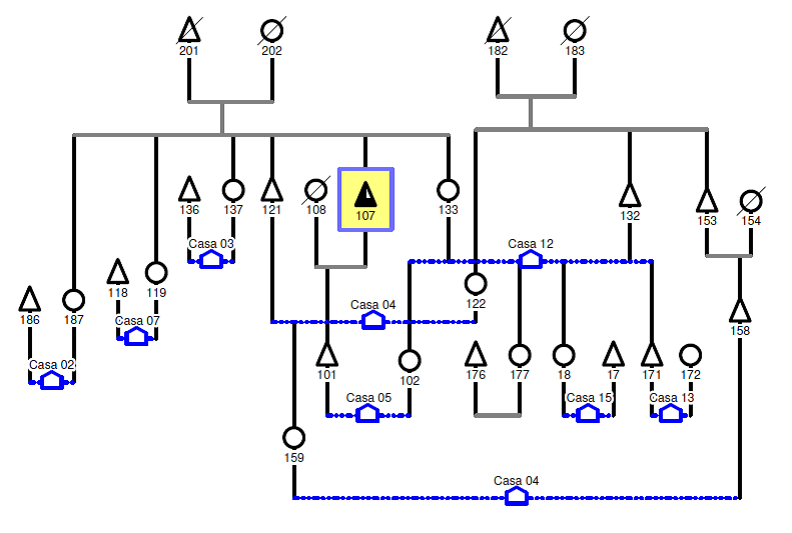
\includegraphics[width=\textwidth]{./img/026}
% \caption{Laços de afinidade e filiação do \textit{kopot} centrado
% em Firmino (ego)}
% \end{figure}

% \begin{figure}
% \centering
% 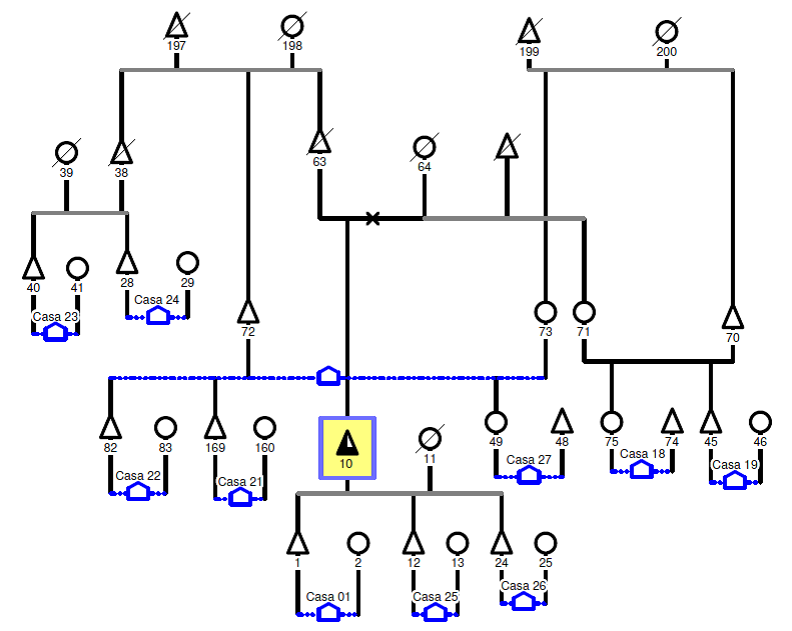
\includegraphics[width=\textwidth]{./img/026k}
% \caption{\textit{Kopot} centrado em Ponciano (ego) por laços de
% afinidade e filiação}
% \end{figure}

Os esquemas de parentesco permitem ver com clareza de que modo as casas
que compõem um agrupamento formam"-se a partir dos laços de afinidade e
filiação orientados em função da pessoa de um dos donos locais. Numa
escala maior, esses agrupamentos parecem seguir uma tendência descrita
por Pozzobon do \textit{líder} do grupo local consolidar laços de parentesco
em torno de si. Em suas palavras, ``vimos que o líder do grupo local é
como um feixe de laços de parentesco próximo, ao qual se ligam os demais
coabitantes através da filiação ou da afinidade. É frequente que o líder
pertença ao grupo agnato mais numeroso''.\footnote{2011, p.\,65.}

Importantes rodas de coca formam"-se todas as noites em torno dos pilões
de Ponciano, Firmino e José para que estes partilhem alimentos
primordiais e saberes com seus cunhados e irmãos. No mesmo sentido, suas
flautas são tocadas para que seus netos e sobrinhos transformem"-se em
guerreiros e casem"-se (\textsc{m17}). Observando o modo como rodas de
coca, flautas Jurupari, vilas e territórios se combinam como atributos
de poder dos donos \textit{Sokw'ät}, é possível retomar \textsc{m17} à luz das
articulações entre esses elementos.\index{26@\textsc{m}17\quad Viagem com as flautas}

Nessa narrativa (\textsc{m17}), Ponciano relembra a viagem que fez com
seu pai, Antônio, à Serra da Iniciação. Após a viagem na Cobra"-Canoa, os
ancestrais caminharam até essa serra para receberem as flautas Jurupari
de \textit{K'e̖g Te͂h}. Em pleno processo de reunião de famílias e instrumentos
sagrados do \emph{sibling} \textit{Sokw'ä̗t} e de clãs afins, esse dono leva o
filho a um local onde todos os grupos e instrumentos estavam reunidos.
Na Serra da Iniciação, os ancestrais comeram coca, beberam \textit{caarpi} e
dançaram com as flautas. De lá, rumaram para as diferentes regiões em
que constituíram suas moradas e territórios. Pensando com Lima (2005), o
processo de formação de \textit{Ta̗t"-Dëh} se dá através de um desdobramento de
relações de similaridade e de alteridade no espaço social, criando um
\emph{socius} onde uma multiplicidade de outros (\textit{yo̖h däh} -- ``gentes de
outras terras'') se situa como o lado de fora do sistema, enquanto uma
multiplicidade de grupos similares (\textit{bab'däh} -- ``donos da terras'') se
situa como seu lado de dentro (2005, p.\,48). As relações internas
expressas pelos \textit{kopot}, pelas rodas de coca ou pelas cerimônias de
Jurupari parecem indicar uma lógica da \textit{suplementaridade} entre os
\textit{donos da terra} e as \textit{gentes de outras terras} que constitui
relações de exterioridade necessárias à autoconstituição da aldeia.

\emph{Caminhar com as flautas} mostra"-se um modo de ação que, ao longo
do percurso, cria caminhos e territórios, e faz surgirem \textit{afastamentos
diferenciais no seio da sociedade}.\footnote{Lima, 2005, p.\,49.} Dispersando"-se
com suas flautas ou reunindo"-se novamente, os membros do \emph{sibling}
\textit{Sokw'ä̗t} consolidam o novo assentamento como um ponto nodal para o
convívio e a vida ritual. Eles mantêm seus caminhos e domínios como
linhas de fuga que os permitem alternar a sociabilidade da aldeia com
períodos de atividades produtivas em suas terras afastadas. Trama de
caminhos, a comunidade compõe a textura do mundo vivido.

Retirar as flautas Jurupari do igarapé, caminhar com elas até a maloca
para dançar em torno do Lago de Leite faz com que os múltiplos
deslocamentos dos ancestrais ao descerem da Serra da Iniciação, as
mudanças dos antepassados \textit{Sokw'ä̗t}, suas brigas, batalhas e
reaproximações se articulem através dos movimentos e timbres das flautas
para transformar os rapazes em guerreiros em plena paisagem da criação.

\index{26@\textsc{m}17\quad Viagem com as flautas}
Entendo que, na dança das flautas, os espaços da aldeia, os territórios
clânicos, as relações sociais e os caminhos percorridos pelos grupos
fazem da paisagem da criação uma trama complexa das múltiplas paisagens
e espaços vivenciados por cada indivíduo ao longo de sua trajetória de
vida. Os cemitérios mencionados por Poncino (\textsc{m17}) são o ponto
de partida para a diferenciação de domínios territoriais originários
entre os clãs, que faz com que aqueles que sejam de \textit{outras terras}
devam aceitar o papel de \textit{acompanhantes} e \textit{apanhadores}, trabalhar
roças distantes e pescar em igarapés com poucos peixes. Constroem suas
casas próximas ao homem de referência do clã local, sentam"-se nas rodas
de coca desses donos e estabelecem seus laços em torno da reciprocidade
matrimonial e ritual. Em muitos sentidos, a grande aldeia ganha os
contornos de uma Serra da Iniciação, onde pessoas de clãs diversos se
reúnem para sentar"-se nas rodas, dançar com as flautas Jurupari e
separar"-se para caminhar e habitar novas paragens. Seguindo Lima,
caminhar com as flautas faz com que a distância espacial faça surgirem
tantas perspectivas quantos forem os caminhos, ao mesmo tempo que os
\textit{kopot} e rodas de coca integram as partes através de relações de
complementariedade.

\section{Pilão"-Jurupari}\label{piluxe3o-jurupari}

Quase um mês depois de meu pedido para que Miguel fabricasse um pilão, o
objeto ficou pronto. Dado o trabalho intenso que a produção exige,
troquei com o artesão uma grande quantidade de bens como redes,
lanternas, bacias, baldes, anzóis e alimentos, como forma de pagamento.
\textit{Me̗y pö̗g nu̗p pu͂'u͂k tö̖k, bɨ̗' hisa̗p!}, ``custa caro esse pilão de coca, dá
muito trabalho para fazer!'', justificava para enfatizar a necessidade
de retribuí"-lo bem pelo esforço empreendido. Acompanhei o trabalho
diariamente fazendo visitas à sua casa para descrever bem os
procedimentos de carpintaria de corte, modelagem, escavação e polimento
da peça. Artesão competente, foi Miguel quem produziu os pilões de coca
de seus cunhados, os donos Firmino e José. Dadas suas habilidades
reconhecidas, além dos pilões de coca, ele recebe encomendas de muitas
famílias para fabricar os pilões de cozinha com os quais se trituram a
carne assada e a pimenta seca.

No dia 28 de agosto de 2011, Miguel acordou cedo e caminhou por algumas
horas pela trilha de sua roça. Levava o machado de um de seus cunhados
apoiado no ombro para tombar o tronco maciço do \textit{säsäw dö̗},
``pau"-brasil'' \emph{Sickingia tinctoria}). A árvore, não muito grande,
encontrava"-se numa área de solo úmido, próxima a um igarapé. Diante
dela, o artesão e seu filho mais velho, Pedro Paulo, demoraram algumas
horas para conseguir derrubar o tronco e cortar o pedaço que seria a
matéria prima para a fabricação do pilão. A medida foi tirada a partir
do corpo de Miguel, tomando como parâmetro o comprimento de sua perna
(chão até a coxa). Uma vez cortado o tronco, pai e filho levaram"-na para
casa. Nos primeiros dias, o trabalho ainda envolveu o uso do machado
para extrair o excesso de madeira. Pouco a pouco, o polimento da peça
com o terçado foi dando a forma cilíndrica ao objeto que, dia após dia,
passou a ser perfurado com um \textit{pica"-pau}, instrumento de carpintaria
semelhante a um enxó.

A fabricação evolveu a participação de filhos, netos e genros de Miguel
que, sempre que podiam, iam trabalhar um pouco na perfuração do pilão.
Nos períodos em que esculpia a peça, Miguel tomava conta dos netos
pequenos, filhos de Pedro Paulo. As crianças divertiam"-se ao ajudar o
avô em sua produção. Foram elas que sopraram a fumaça do breu
incandescente introduzido pelo artesão para vedar o tubo, tão logo
concluídos os processos de polimento e escavação. Miguel demorou ainda
alguns dias para fabricar o socador, pau que acompanha o tubo para
triturar os alimentos. Quando finalmente concluiu a produção, ele
carregou o objeto pesado até a casa onde eu estava alojado, recebeu o
restante do pagamento e disse que tinha fabricado um pilão bonito que
permaneceria resistente para que meus futuros filhos e netos, ao
envelhecer, pudessem preparar sua coca em São Paulo. O artesão envolvia
a todos num engajamento processual e relacional com a materialidade do
pilão, condensando e misturando histórias nas propriedades da madeira
que iam aos poucos dando forma ao objeto

Mal Miguel colocou o pilão no chão, Ari, seu sobrinho (\textsc{zs}), pegou o tubo
com as duas mãos, aproximou"-o da boca e começou a dançar como se tocasse
uma flauta Jurupari. Atentos à paródia, os rapazes, que estavam sentados
comigo estudando violão, começaram a gargalhar. Ari seguiu fazendo os
passos de dança e imitando o som do Jurupari até que não aguentou mais,
largou o pilão e começou a rir. Como Ari, muitos dos rapazes presentes,
iniciavam, nos últimos anos, sua participação nas cerimônias das
flautas. Esses jovens \textit{Sokw'ä̗t} participaram da dança do Jurupari que
presenciei. Imagino que a graça da piada tinha a ver com o fascínio
exercido pela experiência vivenciada. A graça que a figura de um
\emph{pilão"-Jurupari} evocava diz respeito, a meu ver, às diferenças
existentes entre esses dois instrumentos e entre as pessoas que
experienciam, prática e processualmente, as potências e histórias que
fluem a partir da materialidade dos pilões e das flautas.

A fabricação de um novo instrumento Jurupari assemelha"-se em muitos
aspectos ao nascimento humano. Após um período de jejum e banhos
constantes, o artesão dirige"-se à mata à procura de uma \textit{pu̖p tëg},
``paxiúba'',\footnote{\textit{pu̖p tëg}, certo tipo de paxiúba (palmeira da
  família das arecáceas, \emph{Socratea exorrhiza}). Cf. Ramirez (2006).}
encontrada em áreas afastadas da aldeia. Geralmente será acompanhado por
um grupo de rapazes interessados em aprender os procedimentos adequados
à fabricação do instrumento. A palmeira é encontrada nos igapós ou
margens de igarapés, áreas alagadas da floresta. É considerada uma
árvore de porte mediano, sustentada por um feixe cônico de raízes
adventícias recobertas por espinhos curtos e grossos. Constantemente, o
artesão dirige"-se ao local onde tombou a árvore para escavar e raspar o
tronco. Diferente da fabricação do pilão, o trabalho é realizado na
mata, distante das mulheres e crianças, devido aos perigos envolvidos na
fabricação. Um terçado e um enxó são os instrumentos utilizados pelos
artesãos para esculpir as peças. Macho e fêmea são feitos a partir do
mesmo tronco e costumam ter proporções semelhantes. Comparando passagens
da mitologia barasana com características botânicas da paxiúba,
Hugh"-Jones chama a atenção para o caráter mediador dessa palmeira que
cresce num terreno alagado e é usada para construir instrumentos que
permanecem enterrados no rio para, durante os rituais, serem montados e
trazidos para a maloca:

\begin{quote}
Os próprios instrumentos são feitos de partes do tronco da palmeira de
paxiúba, assim como todos os instrumentos de Yurupary. De acordo com os
mitos do Yurupary, essa palmeira cresceu a partir das cinzas do corpo
queimado de Yurupary. A alma de Yurupary {[}\ldots{}{]} penetrou a
palmeira durante seu crescimento e a partir dela ascendeu ao céu.
{[}\ldots{}{]} Os instrumentos He também estabelecem mediação entre a
terra e a água, devido ao fato de serem mantidos submersos nos rios,
sendo trazidos para a terra seca para o uso. A passagem da água para a
terra, e da floresta, onde são mantidos, para a maloca, onde são
utilizados, sinaliza também a passagem da morte, estado inerte, para a
vida, enquanto um estado ativo.
\end{quote}

\index{26@\textsc{m}17\quad Viagem com as flautas}
A versão mítica barasana mostra"-se como uma transformação de
\textsc{m17} com as flautas Jurupari surgindo do corpo queimado de uma
Anaconda, um ser da água, e não de \textit{Bisi̗w}, um ser da mata. Creio que
seja possível ver também o caráter mediador das flautas num sentido
próximo ao explicitado por Hugh"-Jones. Após a saída da \textit{água, do rio,
da cobra} (\textsc{m13})\index{22@\textsc{m}13\quad A dádiva da coca e do tabaco}, os ancestrais hup caminham pela mata e sobem
até o topo da Serra da Iniciação, onde recebem as flautas
(\textsc{m17}). Ao longo do percurso a saída da água, a caminhada pela
mata e a escalada ao topo permitem entender a mediação das flautas que,
como os ancestrais, são tiradas da água, seguem pelo caminho até a
maloca e lá circulam como no topo da Serra da Iniciação (ver
\textsc{m18}). Instrumentos e ancestrais tramam seus caminhos e
condensam suas histórias nos gestos e propriedades materiais do
Jurupari.\index{26@\textsc{m}17\quad Viagem com as flautas}\index{27@\textsc{m}18\quad O \textit{caarpi} do Tamanduá}

Quando os corpos do trompete e da flauta estão prontos, o artesão sopra
o breu para vedá"-los de forma semelhante ao procedimento realizado na
fabricação do pilão. O breu amolecido é passado nos lados externo e
interno do tubo para garantir o timbre adequado ao instrumento.
Murmurando palavras para um pedaço de breu ou para um cigarro, o artesão
executa o \textit{hã̗wäg bi'i̖d}, ``encantamento do sopro vital'', e o \textit{ha̖t
bi'i̖d}, o ``encantamento de nominação''. O xamã desloca"-se como \textit{hã̗wäg}
ao Lago de Leite, chama o ancestral cujo nome será dado à flauta e,
sentado em seu banco, concentra a pessoa"-sopro distribuída pelas moradas
(\textsc{b6})\index{ag@\textsc{b}6\quad \textit{Te͂h Bi'i̖d}\break Benzimento do filho}. A ação xamânica traz o instrumento à vida como um
ancestral através de um processo semelhante àquele que faz do
recém"-nascido um ser humano. O timbre do instrumento é o resultado da
destreza do artesão, bem como das características singulares da
pessoa"-sopro ancestral. Como aponta Cabalzar (2010, p.\,54), ``a
nominação (benzimento de nome) garante às pessoas a obtenção de certas
capacidades vitais essenciais, sem as quais elas não crescem nem
adquirem força ao longo da vida''. Timbre e nome são atributos da flauta
sempre ressaltados pelos tocadores para descrever a beleza, a magnitude
do som e o poder do instrumento. As ações xamânicas de nominação e
concentração do \textit{hã̗wäg} devem ser realizadas por um ancião agnato ao
ancestral"-Jurupari que será trazido à vida como uma pessoa hup pelo
sopro de seus descendentes, durante as danças.

Muitas vezes, sentado na roda, Ponciano dizia que, ao olhar e ouvir o
pilão, se lembrava de seu pai e se entristecia. Qualquer dia jogaria o
triturador no rio, como já devia ter feito quando Antônio morreu. Em
\textit{Ta̗t"-Dëh}, o pilão de Ponciano em torno do qual nos reuníamos todas as
noites, pertencera a seu pai, ao contrário os pilões de Firmino e José,
fabricados por Miguel. Diferente da flauta, o pilão não é benzido para o
uso e, assim, não possui nome ou sopro vital. Seu uso não é tão marcado
quanto o dos pares de flautas. É geralmente manipulado pelos
\textit{apanhadores}, mas pode também ser socado pelos \textit{donos}. Apesar de
poderem ser transmitidos de pai para filho, são muitas vezes jogados no
rio quando o dono morre. Novos pilões são fabricados para que os
descendentes adultos comam coca com seus afins.

Dessa perspectiva, creio que pelo ato de nominação da flauta o xamã não
dá a vida aos instrumentos, fazendo com que a vida passe a estar na
coisa, mas revela o fluxo generativo que traz o objeto e as pessoas à
existência por sua participação dinâmica e mútua num mesmo campo
relacional. As memórias evocadas pelo uso do pilão reestabelecem um
fluxo generativo de sua materialidade que produz o encontro entre sua
história como artefato fabricado e utilizado por antepassados num tempo
pretérito e o preparo da coca atual pelos descendentes que, através de
seu engajamento com o pilão, \textit{crescem nos saberes} ao relembrar e
benzer pelas palavras e sopros. Utilizado todas as noites para preparar
a coca e para chamar os senhores habitantes de \textit{Ta̗t"-Dëh}, o pilão reúne
a todos num modo de ação que gera a vida ``{[}\ldots{}{]} através do
contínuo da vida orgânica, sabendo que essa vida, ela mesma,
estabelece"-se pela geração contínua do fluxo das matérias''.\footnote{2000,
p.\,31.}

Entendo que a aproximação das ações rituais da cerimônia do Jurupari e
das rodas de coca a partir do pilão"-Jurupari ajude a entender como
jovens e anciões se situam num campo de relações com esses artefatos que
se tornam índices de seus pensamentos, intenções e capacidades
corporais. Segurando o pilão de um branco como se fosse um Jurupari, Ari
divertia a todos por dar ao triturador o \emph{status} de instrumento
musical de sopro. A paródia de Ari zombava dos próprios rapazes,
desconhecedores do xamanismo, tão jovens que não sabiam nem o que fazer
com o pilão. Inversamente, explicitava que o pilão era o Jurupari dos
velhos para tocarem sua coca. Certamente, fora esse jogo que levou o
artesão Miguel a sentar"-se ao meu lado para fumar um cigarro e rir com
os rapazes. Afinal, tinha fabricado um pilão para um branco que,
estranhamente, comia coca, se interessava pelo xamanismo e pela dança
das flautas.

\section{Pessoas"-sopro}\label{pessoas-sopro}

Conversando com Evaldo sobre as flautas"-Jurupari, ele me explicou que o
sopro que habita os tubos durante a dança deve partir de um músico cujo
nome emane de seu ancestral"-Jurupari homônimo. Como visto acima, cada
conjunto de Jurupari tem seu dono que transmite a posse e os cuidados de
suas flautas a seus filhos. Constituem, assim, o patrimônio de uma
linhagem clânica específica. Durante as danças, juntam"-se os
instrumentos de linhagens ou clãs distintos para circular pela maloca.
Refletindo sobre as palavras de Evaldo, creio poder dizer que enquanto a
patrilinearidade é um princípio fundamental para a transmissão dos
instrumentos, a \emph{performance} parece expressar a importância de
\textit{grupos de descendência corpórea}, que relacionam pessoas por meio da
identidade corporal e do continuo da mesma substância corporal que
atravessa ancestrais e descendentes.

Com o envelhecimento, o ``ancião'', \textit{wähä̗d}, começa a ter dificuldade em
soprar a flauta e dançar com ela durante horas na maloca. Os senhores
dão lugar para que novos flautistas comecem a manejar os instrumentos
durante a cerimônia. Além do nome \textit{döhö d'äh}, ``sopros'' ou
``pessoas"-sopro'', as flautas são também chamadas de \textit{wähä̗däh},
``velhos'' ou ``antigos''. De modo interessante, os senhores deixam de
dançar ao mesmo tempo em que passam a pertencer a uma categoria que
engloba os instrumentos, antepassados distantes tidos como os primeiros
ancestrais de uma linhagem clânica. Paralelamente, a interrupção da
execução das melodias do Jurupari acompanha a intensificação da prática
dos \textit{bi'i̖d}, ``sopros'', a partir do tabaco e outras substâncias para
proteger e fazer seus filhos crescerem sem doenças (\textsc{b2}). É
nessa fase da vida que os homens começam a frequentar as rodas com
assiduidade e a manusear o pilão para partilhar a coca e as palavras.
\index{ac@\textsc{b}2\quad \textit{Hũ̖t bi'i̖d}\break Benzimento do tabaco}

No que diz respeito à estrutura física, o envelhecimento leva à perda da
dureza da pele e dos ossos, o que pode ser visto como um processo de
\textit{amolecimento corporal}. Sem conseguir soprar as flautas Jurupari, os
anciões começam a não ter mais o corpo envolto pela casca dura das
árvores (\textsc{b1})\index{ab@\textsc{b}1\quad \textit{Pũ'ũ̖k bi'i̖d}\break Benzimento da coca} (\textsc{b5})\index{af@\textsc{b}5\quad \textit{Ti̖wi̖t hamap bi'i̖d ta'}\break Benzimento dos caminhos}. Ao longo da vida, a pele e os ossos
das pessoas hup vão se tornando progressivamente mais duras, atingindo o
auge de resistência na maturidade. Os jovens possuem \textit{corpos moles}
que ainda não foram endurecidos o suficiente para possuírem a
corporalidade do guerreiro (\textsc{m17})\index{26@\textsc{m}17\quad Viagem com as flautas}. Como aponta Reid (1979,
p.\,151), ``De modo mais geral, contudo, a iniciação é um processo por
meio do qual os jovens atravessam o estágio que os Hupdʉ chamam `aqueles
de corpos moles, não totalmente formados' ou adolescência''. Em ambos os
casos, jovens e velhos estão aquém e além da pele"-casca maciça. Possuem
cercas frágeis que não conseguem se erigir como barreiras para as
lanças, espinhos"-dardos ou tábuas culinárias, afecções patogênicas das
Gentes"-Cobra, Gentes"-Árvore e demais seres malfazejos.

Enquanto o bebê precisa passar por processos de resfriamento e
endurecimento, sendo açoitados em cerimônias rituais, caminhando pelas
trilhas, alimentando"-se com a carne de animais de couro duro ou sendo
benzidos continuamente por pais e avós, os rapazes vão tornando"-se \textit{u͂h
me̗h d'äh}, ``guerreiros'', cuja característica física principal é a
rigidez da pele e dos ossos. Em sua descrição, Reid ressalta que, na
divisão das partes do instrumento Jurupari, elas são designadas como
boca, pele, osso etc., o que explicita a analogia entre as flautas e o
corpo humano,

\begin{quote}
Um pouco antes do início do ritual, os convidados pegam suas cargas de
frutas da floresta e lá eles constroem os trompetes Jurupari a partir da
casca e do tronco de várias árvores. As palavras utilizadas para
descreveras várias partes do trompete são pele, osso, boca etc., o que
aponta que essas entidades representam corpos. Uma vez construídos esses
corpos, eles são penetrados pelas sombras ou fantasmas das gentes do
nascimento (ancestrais), e nesse estado são perigosos, pois estão
repletos de essência quente.\footnote{Reid, 1979, p.\,280.}
\end{quote}

Segundo o pesquisador, esses corpos construídos e formados pela boca,
ossos e pele se tornam plenos de energia quente e perigosa quando, ao
longo da dança, são penetrados pela \textit{sombra} ou \textit{fantasma} dos
ancestrais. Na cerimônia das flautas, os açoites fazem com que as peles
dos rapazes fiquem duras como as madeiras duras do pau"-brasil e da
paxiúba. O endurecimento da pele e a rigidez dos movimentos verticais da
dança são ações que se combinam nessa \emph{performance}. Atravessando
os corpos de dançarinos e ancestrais a vida é gerada como um contínuo
entre pessoas que possuem graus distintos de dureza e pulsação
respiratória.

``O certo é colocar três pimentas verdes, uma debaixo da língua e as
outras duas uma de cada lado da boca'', contou Américo quando
conversávamos sobre os perigos do Jurupari. A dança das flautas pode não
só gerar cura e proteção, como também causar doenças e sofrimento.
Afinal, com as flautas, \textit{Bisi̗w} fez a Humanidade \textit{sofrer como ele
sofreu} (\textsc{m15})\index{24@\textsc{m}15\quad \textit{Bisi̗w}, o devorador de rapazes}. Todos aqueles que participaram da cerimônia que
presenciei partilharam, pela manhã, as ardidas pimentas benzidas. É
preciso lembrar que as flautas compunham o corpo \emph{artefactual} de
\textit{Bisi̗w}. Ossos do corpo queimado desse ser, os instrumentos são uma
matéria plena de energia quente que precisa ser manuseada com cuidado.
Se, após o confronto com a presa na caça, o homem come pimenta para
atenuar a agressividade da batalha, logo depois de terminada a dança das
flautas, os participantes comem pimentas verdes sopradas com o
\textit{benzimento da pimenta} para enfraquecer o calor de seus corpos.
Durante uma roda de coca, Jovino alertou"-me sobre alguns gestos que não
devem ser feitos durante o Dabucuri:

\begin{quote}
Durante o Dabucuri, não pode coçar a cabeça, senão pega piolho. Coça
apenas com um pauzinho. Não pode cruzar os braços, senão vira \textit{o}, um
peixinho pequeno. Antes de chegarem as mulheres, pode pegar o cariçu
para fazer limpeza, porque elas não podem pisar na saliva do Jurupari.
Pode dar ferida na perna da mulher e do homem. Pode dar infecção. Toca o
cariçu e limpa. Na hora da festa, só velho pode comer peixe assado que
pesca no mato. {[}\ldots{}{]} Dá \textit{Sub}, ``ferida'', quando come carne
assada sem benzer durante a festa. Não pode assobiar nem gritar, senão
dá cárie. Não pode encostar na mulher, porque ela pode sentir o cheiro
da flauta.\footnote{Jovino, 24 de agosto de 2011.}
\end{quote}

É preciso limpar a maloca soprando as flautas cariçu para neutralizar a
afecção patogênica da saliva do Jurupari. O contato dos dedos com a
cabeça torna o couro cabeludo suscetível à presença de piolhos. O
assobio e o grito degeneram os dentes pelas cáries e o contato corporal
com as mulheres deve ser evitado para que não sintam o odor das flautas
impregnado nos homens. Como destaca Reid (1979, p.\,282), ``Os Hupdʉ são
bastante explícitos quanto ao fato de que praticar rituais faz todas as
pessoas crescerem, ao regenerar a alma dentro delas, e dizem que deixar
de praticá"-los causa doenças, deterioração e morte''.

Assim, a cerimônia do Jurupari revela"-se um perigoso manejo de potências
que podem agir como um feitiço, causando metamorfoses, feridas,
coceiras, dentre outros males. Atingem a pessoa em seu envoltório"-cerca
corporal ou nos dentes que, expostos à energia quente das flautas, se
abrem e/\,ou se desfazem em feridas que levam também à flacidez e ao
amolecimento"-putrefação corporal. Do contrário, o manejo correto dessas
potências primordiais envolve o uso das flautas para benzer as frutas
depositadas no centro da maloca e os açoites com ramos de ingá, ações
que fazem crescer e endurecer. Quer pelos açoites com ramos de ingá,
quer pelas águas"-celestes da Serra Grande, os corpos tornam"-se rijos com
a ação de substâncias frias. Dependendo do modo como as flautas são
utilizadas, a dança pode levar tanto à proteção como ao amolecimento e
adoecimento. Revela"-se a importância do equilíbrio entre a energia
quente dos tubos rijos e do caxiri e a energia fria dos ramos de ingá e
da água.

Enquanto tocam as flautas, os rapazes são inseridos numa forma de
interação sensorial direta e potencialmente perigosa com os
ancestrais"-Jurupari. Artefatos"-pessoa, os corpos das flautas passam a
ser a referência para a fabricação dos corpos dos participantes. A
harmonização entre sopros e resistência física dos \textit{jovens de corpo
mole} com os \textit{ancestrais Jurupari de corpo duro} se dá no contato com
a pele, ossos e boca desses primeiros hup. Como o feto adornado no
ventre materno, a postura e a gestualidade aproximam o neófito e o
antepassado que, apesar de extremamente velho, é um guerreiro maciço.
Nesse sentido, os corpos humanos são percebidos a partir de um
\emph{devir"-jurupari} que é igualmente um \emph{devir"-guerreiro}.

\index{ag@\textsc{b}6\quad \textit{Te͂h Bi'i̖d}\break Benzimento do filho}
Através de seus movimentos e da atenção que mantêm, os rapazes
desenvolvem uma sensibilidade íntima e pessoal para outros modos de ser
como aqueles dos primeiros Hupd'äh e dos velhos. Com a análise de
\textsc{b6}, foi possível entender que, evocando o nome do ancestral, o
xamã retira as parcelas distribuídas da pessoa desse antepassado. Se o
sopro concentrado do antepassado dá a vida ao bebê, pelo toque da flauta
e movimentos de danças, os descendentes trazem à vida os antigos com a
essência vital que receberam como uma dádiva ao nascer. Refletindo com
Lima, o \emph{feto adornado} e o \emph{rapaz flautista} parecem deixar
ver a concentração do sopro vital e do sopro das flautas como processos
de individuação da pessoa que se torna um ser para si e para outrem. Na
dança, as linhas"-vitais de antepassados e descendentes se interpenetram,
atravessam"-se através dos movimentos e das ações \emph{progenerativas}
que compõem um campo relacional em que seres emergem cada qual com suas
formas, capacidades e disposições para fazer crescer e fortalecer os
rapazes.

Tomando como referência a comparação de Viveiros de Castro entre
\textit{totemismo} e \textit{sacrifício}, creio poder dizer que soprar a flauta
revela"-se uma ação de \emph{transdução} que corporifica simultaneamente
as pessoas do descendente e do ancestral homônimos no fluxo contínuo da
respiração e gesto musical. Diferenciados enquanto polos pressupostos
como autossemelhantes, o sopro, um gesto de indução ou transdução, cria uma
zona, um momento de indiscernibilidade entre eles, acionando ``relações
intensivas que modificam a natureza dos próprios termos, pois `fazem
passar' algo entre eles'' (p.\,89). As ações de \emph{soprar as flautas}
e de \emph{concentrar a pessoa"-sopro distribuída} realizadas pelos
dançarinos e pelos xamãs parecem regenerar a vida pela energética do
contínuo entre \textit{wähä̗däh}, ``velhos'', e \textit{te̖͂h d'äh}, ``filhos'', por meio
da transdução entre sopros, corpos e objetos (\textsc{b2}). Na
energética do contínuo desses \textit{grupos de substância} todo cuidado é
pouco, pois o endurecimento e crescimento são o reverso da degeneração e
da morte.\index{ac@\textsc{b}2\quad \textit{Hũ̖t bi'i̖d}\break Benzimento do tabaco}

%\section{Cuias de caxiri}\label{cuias-de-caxiri}

\section{O caxiri das manivas}\label{o-caxiri-das-manivas}

À medida que os dançarinos começam a se aproximar da maloca, o caxiri
\textit{po̗ho̗y}, ``ferve'', cada vez mais. O gosto doce das primeiras cuias
oferecidas passa a ser marcado pelo amargor da bebida em seu ponto forte
e ideal para o consumo. Com apenas poucas cuias, dançarinos e
carregadores embriagam"-se. Suas gargalhadas e vozes tomam conta da
palhoça enquanto as flautas estão quietas no chão. O caxiri é uma bebida
preparada pelas mulheres através de um processo que envolve uma série de
procedimentos e etapas de trabalho com a maniva.

Dentre as ações fundamentais para o preparo da bebida, podem ser
destacadas a colheita dos tubérculos, a extração das cascas, a lavagem e
hidratação nos igarapés, o uso do ralador para triturar a massa, o uso
do tipiti para espremê"-la, o longo cozimento da manicuera. O calor do
fogo livra o líquido de sua toxidade permitindo que a manicuera seja
adicionada à massa feita a partir de beijus torrados, mastigados,
cuspidos e raspados na canoa de caxiri. À mistura podem"-se adicionar
sumos de fruta como a pupunha, o ingá, a cucura, ou massas como a de
batata doce, dentre outras. Para intensificar a fermentação costuma"-se
colocar caldo de cana ou pacotes de açúcar. Depois de terminada a
mistura, a preparadora tampa a canoa com folhas de bananeira para que a
bebida fermente até atingir o ponto de consumo. Caxiris preparados no
intervalo de um dia são chamados \textit{ɨ̗b' dëh}, ``caxiris vivos'', que serão
sempre menos fortes e mais adocicados que os \textit{tä̗w hu̗ptök}, ``caxiris
bravos'', cujo tempo de descanso varia de dois a três dias. O preparo do
caxiri e seu oferecimento nas festas são atividades femininas que
definem a posição ocupada pelas mulheres no campo de interações da
maloca.

Em março de 2012, caminhei com Isabel e Américo para as roças da
família, durante dias seguidos. Minha anfitriã levava seu aturá, pois
colhia manivas e algumas batatas doces para o preparo do \textit{kiwi̗' dëh},
``caxiri de batata doce''. O dia da festa de caxiri aproximava"-se, e
ela, esposa do capitão, precisava produzir uma grande canoa para
\textit{kɨhsä̗t}, ``estar à frente'', e superar a produção de suas vizinhas.
Afinal, não queria que as outras maculassem sua fama de mulher
trabalhadeira. Quando chegamos, Isabel guiou"-me pelas muitas \textit{kopot},
``vilas'', que há em suas roças. As manivas são plantadas em grupos que
se espalham por toda a clareira do espaço agrícola. Numa parte estão as
\textit{kaya̖k ti̖g töhö̗}, ``manivas brancas'', mais utilizadas para a produção
de farinha e beiju. Apesar de haver alguns tipos de \textit{maniva branca}
utilizadas para o preparo do caxiri, o mais comum é colher as \textit{kaya̖k
dö̗}, ``manivas vermelhas'', em grande quantidade, para o preparo da
bebida.\footnote{Há tipos de \textit{manivas vermelhas} utilizadas para o
  preparo de farinha e beijus (\textsc{ssl}, 2012).} Foi às \textit{kopot}, ``vilas'',
dessas manivas que nos dirigimos naquela manhã. Comentando sobre o
trabalho feminino, Reid enfatiza o caráter árduo da lida com as manivas
e a pouca especialização entre as agricultoras,

\begin{quote}
As mulheres geralmente colhem, capinam e replantam pedaços de
aproximadamente 4x4 metros em algumas horas. Depois disso, retornam ao
porto próximo à casa. Todas as mulheres se reúnem nesse local,
banham"-se, banham seus bebês e lavam os tubérculos de mandioca.
{[}\ldots{}{]} Na maior parte dos dias, o cultivo e processamento de
mandioca leva entre seis e nove horas, sendo o restante do tempo
preenchido pelas atividades domésticas. Do modo como pude observar, há
pouca especialização individual entre as mulheres, embora as mulheres
mais velhas possam preparar a farinha de mandioca e, especialmente,
tramar cestos de carga muito mais rápido que as mulheres jovens.\footnote{Reid,
1979, p.\,39.}
\end{quote}

De certo modo, enfatizando não a especialização das agricultoras segundo
suas competências técnicas, mas sim o modo como fazem crescer as plantas
de acordo com a origem, a sociabilidade e as formas de interação e
consumo das manivas que coabitam as roças, talvez seja possível perceber
o caráter singular desses arranjos produtivos que revelam as habilidades
de cada mulher para criar e desenvolver as plantas e os filhos.

Como me explicou Américo, cada \textit{vila} agrupa apenas as manivas de
mesmo nome e origem que são plantadas uma próxima à outra. Sentando"-se
no meio da plantação, Américo mostrou a \textit{vila} onde o casal cultiva um
tipo de maniva branca que foi transmitida a Isabel por sua sogra. Fora
essa maniva que fizera o capitão crescer forte e sem doenças e, por
isso, seus filhos sempre comiam os beijus preparados com as plantas
dadas pela mãe de Américo. Quando se casou, Isabel ganhou de sua própria
mãe em \textit{Pi̖j"-Dëh} tubérculos de diversos tipos de maniva para que
iniciasse sua plantação nas terras de \textit{Ta̗t"-Dëh}. Cultivados há décadas,
esses ramos deram origem a agrupamentos que hoje garantem a colheita
para o preparo de farinha, beiju e caxiri, pela família.

Desse modo, a roça pode ser descrita como uma grande aldeia formada por
\textit{vilas} de manivas que podem ter sido trazidas de outras comunidades
ou transplantadas das roças das mães e tias das agricultoras.
Interpretando a relação entre as mulheres barasana e o cultivo de
manivas, C. Hugh"-Jones\footnote{1979, p.\,173.} ressalta que ``a confiança que se
pode ter em uma plantação sugere que a mulher harmoniza"-se com a
mandioca, em vez de empregar seus poderes físicos e mentais contra
ela''. No caso, o agrupamento das manivas em \textit{vilas} que assemelham a
roça a uma aldeia ou a um grupo local parece apontar para um modo de
habitação dos tubérculos muito próximo àquele dos arranjos sociais hup.
Nas vilas, as manivas diferenciam"-se também como aquelas que são \textit{de
outras terras} e aquelas que são \textit{da terra}, dependendo do modo de
transmissão. Cada arranjo produtivo é o resultado da história de vida da
agricultora que, através de sua produção, cuida de seu marido e dos
filhos, fazendo"-os crescer. Partindo da reflexão de Ingold,\footnote{2000,
p.\,87.} as mulheres hup estabelecem as condições para o crescimento das
plantas e de suas próprias famílias, ``{[}\ldots{}{]} suas atividades
são parte do ambiente para as plantas''.

Em cada uma das \textit{vilas}, as manivas formam rodas de conversa e
oferecem caxiri umas para as outras. ``Se não plantar junto, a maniva
não conversa e não cresce'', dizia a agricultora, orgulhosa de sua vasta
plantação. As vilas e rodas de manivas são arranjadas de modo parecido
ao do plantio da coca, para que os pés conversem e ofereçam cuias de
coca entre si. Não é à toa que as roças de coca são feitas sempre ao
lado de \textit{vilas de maniva}. Além das folhas da maniva proporcionarem o
sombreamento adequado ao crescimento da coca, os tubérculos oferecem
cuias de caxiri aos pés de coca. Satisfeitos com a dádiva, os
\textit{velhos"-coca} retribuem executando encantamentos que protegem as
manivas. A mesma sociabilidade pode ser observada na relação entre as
rodas de maniva e a roça de pimenta que germina sempre próxima.
Igualmente dotadas de habilidade xamânica, as pimentas também benzem as
manivas em troca de cuias de caxiri. Apontando para o chão, Américo
revelou que um imenso Rio de Leite se estende por debaixo da terra e
alimenta as plantas com seu leite e águas"-puras, nutrientes que
possibilitam o crescimento dos vegetais. Como no caso Achuar descrito
por Descola, ``essa pequena população de plantas estabelece em seu meio
aspectos de sociabilidade idênticos aos dos homens''.\footnote{1986, p.\,244.}

Assim, a harmonização da mulher com a maniva revela"-se também em termos
de seus modos de ação e sociabilidade, o que permite ver o processo de
crescimento das plantas a partir de suas analogias com o desenvolvimento
humano, com os encantamentos, com os oferecimentos de caxiri e com o
aleitamento.

Analisando as analogias entre o processo de trabalho feminino com as
manivas, ações rituais e passagens míticas, C. Hugh"-Jones mostra como a
lida com a maniva pode ser vista como uma contraparte feminina às
cerimônias masculinas de Jurupari. Enfatizando aspectos de renovação, de
crescimento e transformação, a antropóloga explicita os paralelos entre
o ciclo vital masculino e o feminino e as etapas de processamento do
tubérculo para o preparo de alimentos e bebidas que dotam as mulheres do
poder de agregar pessoas em torno das substâncias resultantes de seus
trabalhos. Marido e filhos reúnem"-se para comer o beiju e beber o mingau
nas refeições diárias, ao mesmo tempo em que o caxiri cria as condições
para a reunião das famílias na maloca para festejar ou para realizar
Dabucuri. Nas roças das mulheres hup, a convivência das plantas parece
dar"-se de forma ritualizada, já que a reciprocidade entre manivas e coca
se estabelece através da articulação entre uma forma de interação
própria das festas, o oferecimento de caxiri, e outra comum às rodas de
coca, o pedido de benzimento. Seguindo a reflexão de Descola (1986,
p.\,263), ``quando postulamos que as plantas cultivadas são seres
animados, é evidentemente normal tentar estabelecer com elas relações
sociais harmoniosas {[}\ldots{}{]} que servem, igualmente, aos fins das
relações entre humanos''.

Longe da maloca, entre uma colher de coca e uma cuia de caxiri, os
senhores hup divertem"-se nos \textit{hu̗ptök wa̗g}, ``dias de festa de caxiri''.
Nos dias anteriores, apanhadores e donos colhem uma quantidade grande de
folhas para que todos possam comer e conversar durante toda a festa. O
pilão começa a soar no meio da manhã e seu som mistura"-se aos timbres
das flautas pã (cariçu) e, mais tarde, ao volume dos aparelhos de som
estéreo que divertem a todos com os forrós e as guitarradas. Vez ou
outra, um dos senhores levanta"-se, dirige"-se para a maloca levando uma
panela de caxiri já vazia para ser reabastecida pelas mulheres. Tendo a
boca esverdeada, as bochechas cheias de coca e os cabelos desgrenhados,
a entrada dos velhos no salão de baile provoca o riso automático dos
jovens e dos adultos. Na maloca eles ensinam melodias de cariçu aos
flautistas, comentam sobre as roupas, danças e músicas dos mais jovens
e, logo, retornam à roda. As mulheres fazem questão de dar aos senhores
grandes quantidades de caxiri, pois sabem que sua generosidade será
lembrada pelos xamãs quando elas pedirem um benzimento aos \textit{comedores
de coca}.

As festas de caxiri iniciam"-se quando as mulheres começam a trazer para
a maloca panelas plenas de bebida. Os homens já sentados nos bancos vão
recebendo as cuias a eles oferecidas. Não beber tudo de um gole só nesse
momento pode ser uma grave ofensa, já que o caxiri é oferecido pelas
preparadoras como degustação. Depois de virar a cuia, é de bom tom
emitir um sonoro \textsc{ahhhh}!!!, um arroto ou dizer enfaticamente para a
pessoa ao lado: \textit{pë̖' hisa̗p, hu̗ptök pë̖' hisa̗p, na̗w kɨd}, ``caxiri forte,
muito forte, bom demais!''. Mas é claro que apenas receberão tais
elogios aquelas mulheres que possuem maior experiência e habilidade no
preparo. Diz"-se que o caxiri de moças novas é doce e fraco, ao contrário
do caxiri das senhoras, considerado forte, amargo e saboroso. Pessoas de
paladar apurado, aprimorado ao longo de toda a vida, os senhores hup
procuram geralmente as panelas das mulheres mais velhas, pela certeza da
boa bebida.

Depois de circularem com suas panelas pela maloca, as donas do caxiri
sentam"-se em roda próximas à Porta"-da"-Cabeceira. Oferecem cuias umas
às outras e começam a comentar sobre o sabor e força dos caxiris. À
semelhança das rodas de maniva, as mulheres conversam enquanto bebem,
riem e preparam"-se para pegar mais uma vez suas panelas do chão e
fazê"-las circular pela maloca. Durante a dança das flautas, quando os
tocadores se sentam para beber as cuias de caxiri oferecidas pelo dono,
os instrumentos mantêm"-se em repouso no chão, enquanto os músicos
conversam e gargalham. Sentam"-se, assim, da mesma forma que as mulheres
nas festas de caxiri. São os movimentos das panelas de caxiri e das
flautas Jurupari que fazem surgir \textit{lagos de leite} na maloca transformada
na paisagem da criação.

Enquanto o sopro traz à vida os ancestrais"-Jurupari, artefatos"-pessoa
que estabelecem os parâmetros para a fabricação dos corpos dos neófitos,
os úteros femininos são percebidos como panelas ou cuias"-recipientes cheios
de \textit{ɨ̗b' dëh}, ``água"-da"-vida'', líquido que envolve o esperma para gerar
o feto"-sentado. Como no desenvolvimento humano intrauterino, a
\textit{fermentação é uma transubstanciação da bebida}\footnote{Lima, 2005, p.\,295.}
e não é por acaso que chamam de \textit{ɨ̗b' dëh} uma das formas de caxiri com
pouca fermentação. A gestação se dá por um processo análogo ao
cozimento"-fermentação que faz o nascituro crescer como um ancestral hup
dentro da panela, ou cuia. Creio que a aproximação entre flautas Jurupari e
panelas de caxiri revela a articulação entre duas agências fundamentais
para a criação e desenvolvimento da vida. Seguindo Hugh"-Jones, num plano
abstrato, tubos e recipientes relacionam"-se às capacidades e processos
de reprodução. Por um lado, os tubos soprados são uma forma gerada ao
longo dos movimentos da dança que contribui para a expressão da
continuidade entre ancestrais e descendentes pelo sopro vital e pelo
envoltório da pele"-casca que cerca os \textit{bravos guerreiros}. Por outro
lado, as panelas de caxiri fazem da fermentação e do aquecimento
processos importantes para o desenvolvimento do corpo e dos saberes que
nutrem a pessoa através das conversas, danças e viagens. Enquanto os
açoites, banhos e benzimentos parecem resfriar para endurecer
(contenção), o caxiri, a fermentação e os recipientes aquecem para fazer
crescer (expansão).

A sociabilidade das plantas na roça parece delinear"-se a partir de um
campo de interações muito semelhante ao dos dias de festa de caxiri.
Como para os Humanos, as conversas nutrem e fazem crescer as plantas, os
oferecimentos de caxiri garantem a reciprocidade do xamanismo entre
senhores e mulheres, entre a coca e os tubérculos. No evento do Dabucuri
que presenciei, as mulheres receberam como dádiva dos homens uma imensa
quantidade de buritis soprados pelas flautas Jurupari durante a
madrugada. Trazidos à vida pelos descendentes, os ancestrais Jurupari
são \textit{wähä̗d'äh}, ``anciões'', que benzem as frutas com as quais as
mulheres prepararão sumos, águas"-puras para serem bebidas pela família.
Fervidos e ralados, os buritis transformam"-se numa massa que é
adicionada ao caxiri a ser oferecido a todos durante as festas.

Se a vila de maniva leva Américo a lembrar"-se de sua mãe que, com o
beiju preparado a partir dessas plantas, fez crescer seus filhos como
pessoas fortes, a massa de tapioca oferecida pelas mulheres aos homens
explicita a habilidade feminina de fazer crescer os filhos e o marido
através do preparo dos alimentos e dos cuidados com as plantas na roça.
Como as manivas que oferecem as cuias de caxiri à coca, as mulheres
oferecem a massa a um velho xamã, Mandu, em retribuição aos frutos
benzidos pelos ancestrais"-Jurupari. Pensando com C. Hugh"-Jones, é
possível ver em que medida o consumo das substâncias é também um consumo
dos processos míticos, xamânicos e práticos que fazem com que a
sociabilidade das plantas e de humanos ocorram a partir de formas de
interação semelhantes e complementares. O caxiri e a coca são veículos
de interação social que agregam pessoas, plantas e humanos, em torno do
consumo das substâncias, das conversas e dos encantamentos.

\section{A fala poderosa}\label{a-fala-poderosa}

Numa festa de caxiri, depois que as mulheres já tinham abandonado a
maloca com suas panelas, Vicente e João Brasil sentaram"-se um ao lado do
outro. Tinham uma panela de caxiri diante de si e, entre uma cuia e
outra, conversavam intensamente. No momento em que me aproximei, eles me
ofereceram caxiri e disseram: \textit{ɨ̗d pa̗y, nɨ̖h ɨ̗d}, ``fala ruim, a nossa
conversa''. João Brasil explicava ao primo paralelo as ações de um
feitiço. Rapidamente, enfatizaram que essa era uma \textit{fala ruim} em
oposição à \textit{fala boa}, a \textit{fala dos benzimentos} através da qual eles
curam e protegem seus filhos. Segundo eles, precisam conhecer os
feitiços causados pela ação agressiva dos Tukano e de benzedores e pajés
hup de outras regiões para que possam cercar bem a maloca. Só assim não
haverá brigas, envenenamentos ou assassinatos. Mas a força da \textit{fala
poderosa} permite a aquisição de habilidades xamânicas para causar
\textit{döhöy}, ``estragos'', punir ou vingar a morte ou desgraça sofrida por
parentes.

Quando se encontram sentados nas rodas de coca bebendo caxiri, além das
piadas e conversas amistosas, os senhores hup conversam pela \textit{pu̗b ɨ̗d}, a
``fala poderosa'', ou \textit{döh ɨ̗d}, ``fala dos sopros'', por meio da qual
aprendem e ensinam feitiços. Os estragos podem fazer pessoas ou famílias
adoecerem, e até mesmo dizimar aldeias inteiras, impedir a caça e a
pesca devido ao aprisionamento dos animais, e induzir pessoas ao
suicídio. Retomando \textsc{m15}\index{24@\textsc{m}15\quad \textit{Bisi̗w}, o devorador de rapazes}, a queima do corpo de \textit{Bisi̗w} faz
surgirem as flautas Jurupari, mas em meio à sua agonia o ser ancestral
amaldiçoa os Hupd'äh que passam a sofrer com as brigas, os
envenenamentos e as mortes após a vingança dos pais dos rapazes
devorados. Como descreve Reichel"-Dolmatoff (1986, p.\,188) para os
Desana:

\begin{quote}
O fato de que o mesmo sentimento de segurança pessoal também exige, por
vezes, atitudes negativas, é apenas natural. Agressões mágicas para
causar uma desgraça ao próximo, doença ou até a morte são frequentes
entre os Desana e as causas para essas inimizades podem ser múltiplas: a
invasão de um território de caça ou de pesca; um roubo cometido em uma
roça ou, talvez, algum desgosto ocorrido durante uma festa.
\end{quote}

A palavra \textit{döhöy} traduzida pelos Hupd'äh como ``estrago'' ou
``feitiço'' possui a mesma raiz da palavra \textit{döhö}, um dos nomes dados
aos Jurupari. O caxiri extremamente forte que ferventa com a aproximação
das flautas e o caxiri que os senhores hup bebem nas rodas de coca em
dias de festa levam a uma intensificação da energia quente de seus
corpos. Sentados em seus bancos"-de"-leite, os anciões conseguem atingir
esse estado de extrema agressividade sem brigar uns com os outros, um
controle difícil para os mais jovens que, sob o efeito das muitas cuias
de caxiri, começam a se desentender. Como me explicou Samuel, a
agressividade e o aquecimento fazem com que os senhores hup fiquem como
\textit{Wero̗ Hup Te̖͂h}, o Sol, e como o próprio \textit{Bisi̗w} em seu momento de
ódio intenso antes de ser queimado na fogueira (\textsc{m15})\index{24@\textsc{m}15\quad \textit{Bisi̗w}, o devorador de rapazes}. Os
senhores que bebem caxiri não praticam encantamentos e, enquanto
conversam sobre a \textit{fala poderosa}, não podem realizar ações xamânicas
para cercar ou curar, pois suas palavras apenas causarão malefícios aos
outros. Para Buchillet\footnote{1983, p.\,131} as \textit{doenças de feitiço} são
causadas pela realização de encantamentos semelhantes aos benzimentos de
cura e proteção:

\begin{quote}
Por outro lado, os textos foram concebidos para cuidar (encantamentos
terapêuticos) ou para provocar (encantamentos maléficos) esses
malefícios. Esses textos são elaborados a partir de episódios míticos
relativos às situações de criação das doenças. {[}\ldots{}{]} A cura e o meio
de produzir as doenças são transmitidas aos ku͂bu͂ pelas gerações. Os
Desana insistem sempre sobre o fato de que não há \textit{bons ku͂bu͂} ou
\textit{ku͂bu͂ malfeitores}, toda cura é ensinada e aprendida ao mesmo tempo
que seu contrário, encantamentos terapêuticos e agressões fazem parte de
um arsenal terapêutico de todo ku͂bu͂, encantamentos terapêuticos e de
agressões são, portanto, complementares.
\end{quote}

Na explicação dada por meus interlocutores, a \textit{fala poderosa} pode ser
vista como complementar às ações terapêuticas, pois permite aos xamãs
entenderem o mal causado por outrem para poder tratá"-lo, ao mesmo tempo
em que os dota do poder de se vingar, agredindo aqueles que provocaram o
sofrimento. Refletindo sobre a cerimônia de rupari, Reid\footnote{1979, p.\,281.}
afirma que os participantes induzem um estado pleno de energia quente e
extremamente perigoso. Em suas palavras,

\begin{quote}
Desse modo, os Hupdʉ induzem neles mesmos um estado muito quente e
perigoso que leva ao clímax do dia seguinte, quando as mulheres e as
crianças correm da casa e os trompetes Jurupari e as frutas são trazidas
para dentro.
\end{quote}

\index{24@\textsc{m}15\quad \textit{Bisi̗w}, o devorador de rapazes}
Retomando \textsc{m15}, é possível perceber que os males que acometem
\textit{Bisi̗w} delineiam um processo de intensificação de energias e elementos
quentes. O caroço de uacu queimado, que o leva primeiro ao desmaio, em
seguida a uma agressividade intensa que o faz devorar os rapazes vivos.
Em seguida, o caxiri soprado, oferecido pelos pais, embriaga rapidamente
o ancestral que seria, então, queimado vivo. As flautas surgem do
extremo aquecimento de seu corpo pelo caxiri e pelo fogo, num momento de
extrema agressividade e violência que resulta no aparecimento das
doenças, das brigas e dos envenenamentos como modos de a humanidade
``sofrer como \textit{Bisi̗w} sofreu''. Esses males são, portanto, feitiços
causados pela ação maléfica de \textit{Bisi̗w}.

Substâncias plenas de energia fria, os buritis atenuam o calor extremo
da fermentação do caxiri para que, durante as conversas, as palavras
possam fazer crescer sem potencializar a agressividade ou as
enfermidades nos dias de alegria. Como mencionado, os dançarinos
precisam banhar"-se antes de retirar as flautas do rio. Como um Rio de
Leite, as águas do igarapé são compostas pela energia fria que conserva
os instrumentos num estado de resfriamento. É possível ver, então, a
sequência de ações da dança do Jurupari como um manejo combinado de
potências frias e quentes. Os ramos de ingá que ferem as peles dos
rapazes são uma essência fria que atinge a pele mole para endurecê"-la e
moldá"-la. O exercício de controle sobre a agressividade que leva os
rapazes a perseguirem o agressor, mas não a revidar os açoites parece
constituir o contexto relacional para o aprendizado de um controle de
si.

Em meio às cuias de caxiri e às \textit{falas poderosas}, os xamãs
intensificam a energia quente de seus corpos, mas o consumo de coca e a
postura sentada nos bancos de leite mantêm o equilíbrio para que atenuem
ou dirijam sua agressividade contra seus inimigos. Nos encontros
noturnos, a carne e ossos assados e pilados do Velho Cobra são
cuidadosamente misturados com o \textit{pu͂'u͂k"-b'ö̖h}, o ``sal de coca'', obtido
a partir das cinzas das folhas secas de embaúba queimadas. A própria
embaúba recebe o nome de \textit{pu͂'u͂k"-b'ö̖h"-tëg}, ``árvore de sal de coca'',
expressão que a identifica pela sua condição de tempero culinário para o
preparo da coca.\footnote{Em sua análise, Lévi"-Strauss ressalta a
  importância da embaúba (\emph{Cecropia}), uma árvore de tronco oco
  muito utilizada por povos ameríndios para a produção de instrumentos
  musicais como tambores (2004b, p.\,342).} O sal é um condimento pleno
de energia fria que atenua o calor dos alimentos. Da mesma maneira, o
\textit{sal da coca} permite que a coca, uma substância plena de calor,
atinja um equilíbrio térmico e gustativo. Bem temperada com sal, a coca
fica doce como o leite, mantendo certo grau de calor bom para fazer
crescer os saberes, mas fria o suficiente para que os xamãs se mantenham
serenos e falem apenas sobre encantamentos de cura e proteção. Desse
modo, é possível ver como nas cerimônias de Jurupari, nas rodas de
caxiri e nos encontros noturnos há um equilíbrio tenso entre energias
quentes e frias, entre estados de serenidade e violência, cujo domínio
pelo xamã se torna fundamental para que consiga curar, cercar ou
agredir. As festas de caxiri e danças de Jurupari se colocam como formas
de interação perigosas, por envolverem processos coletivos e pouco
controlados em que neófitos, mulheres e homens intensificam
demasiadamente a potência quente e violenta de seus seres.

Muitos dos desentendimentos iniciam"-se em festas de caxiri, indo desde
bate"-bocas até confrontos corporais. Em casos extremos, as brigas podem
levar ao assassinato com os oponentes empunhando terçados ou
atingindo"-se com flechas envenenadas. O envolvimento de grupos em defesa
de ambas as partes pode gerar guerras como as que ocorreram no início
dos anos 2000, em \textit{Pɨ̖͂g"-Dëh} e em \textit{To̗͂h"- Haya̗m}. Essas \textit{u͂h me̗h},
``guerras'', ``batalhas'', de enfrentamento entre clãs oponentes causaram
muitas mortes e culminaram na fissão do grupo local. Comentando sobre as
brigas durante as festas de caxiri, Reid vê nos
conflitos suscitados pelos eventos coletivos e pelo consumo da bebida um
contexto de expressão das tensões, frustrações e ódios entre pessoas e
grupos. Nas palavras do autor:

\begin{quote}
Os Hupdʉ são calmos, quietos e autocontrolados no dia a dia, mas à
medida que a festa se inicia, a casa torna"-se cada vez mais barulhenta
{[}\ldots{}{]} Nos momentos finais da festa ocorrem brigas sérias que
irrompem entre coabitantes, ou entre anfitriões e convidados, terminando
quase sempre em mortes ou em injúrias sérias. {[}\ldots{}{]} Exceto
pelos desentendimentos ocasionais entre maridos e esposas, as brigas
ocorrem somente durante as festas de caxiri ou rituais. {[}\ldots{}{]}
Desejos, frustrações, ciúmes, afetos ou desafetos pessoais e outras
tensões propensas a ocorrer entre grupos pequenos de pessoas vivendo em
intensa intimidade encontram expressão durante as festas de caxiri, ao
passo que são completamente reprimidas no dia a dia.\footnote{Reid, 1979, p.\,135-6.}
\end{quote}

Nos dias de festa de caxiri, depois de beber na maloca, é comum haver
desentendimentos entre rapazes, irmãos entre si, que começam a brigar. O
irmão maior procura repreender o caçula por dirigir"-se
desrespeitosamente às moças, por discutir com um rapaz de clã afim. A
repreensão do irmão maior causa a ira do rapaz, porque, de seu ponto de
vista, apenas o pai pode chamar a sua atenção. Mas mesmo os
enfrentamentos de filhos com pais não são raros durante as festas. As
brigas e pancadas são acompanhadas de perto por mulheres, crianças e
rapazes. Terminam apenas quando o pai ou senhores aproximam"-se,
atendendo aos pedidos desesperados das mulheres, e tentam acalmar a
todos.

De modo diferente, as brigas de mulheres acontecem principalmente entre
aquelas que pertencem ao clã local e suas afins, que são \textit{gente de
outras terras}. Ao longo da festa, as rodas de caxiri das mulheres vão
ficando cada vez mais animadas. Com suas panelas, elas começam a rir e a
falar alto. Quando se levantam, iniciam ``cantos'', \textit{yamido̗'} dedicados
ao homem sentado para quem estão oferecendo o caxiri. Esse deve beber
todo o caxiri da cuia e não pode devolvê"-la enquanto a cantora não
terminar sua canção. Num dado momento, elas levantam"-se e começam a
cantar canções de improviso umas para as outras. As melodias são
aprendidas desde a infância com as mães e avós. Nos versos dessas
trovas, as cantoras afins contam sobre suas vidas em outras terras,
falam sobre seus clãs, suas famílias, seus maridos. Já as \textit{donas da
terra} contam de sua vida, do casamento com maridos de outras terras,
bem como sobre seus filhos, roças e caxiris. Se o diálogo musical for
amistoso, os versos de uma e outra trarão agradecimentos por ajudas e
pela boa convivência. Esses cantos constituem um gênero denominado
\textit{hisösö̗y yamido̗'}, ``cantos alegres''. Entretanto, os desafios podem
culminar em \textit{tä̗w yamido̗'}, ``cantos de ira'', com versos que vão
insultando a oponente através da desqualificação de sua pessoa.
Atacando"-se mutuamente, as cantoras maculam a imagem de boas
trabalhadoras e de boas mães, acusam"-se de roubo, de mau comportamento
etc. As disputas são acompanhadas por outras mulheres e podem suscitar
brigas corporais entre as interlocutoras que terminarão com a
intervenção de um marido ou filho.

Nos encontros noturnos dos dias que se seguem às festas, os senhores
conversam muito sobre as brigas. Comendo coca, procuram entender a causa
e a origem do sopro que fez irmãos verem"-se como inimigos, e
\textit{cunhadas} a porem risco sua boa convivência. Dependendo das pessoas
que se envolveram na disputa e dos motivos que levaram ao confronto, os
xamãs saberão se o causador foi um feiticeiro tukano, ou um xamã hup de
outro grupo local como \textit{Pi̖j"-Dëh} ou \textit{To̗͂h"-Ha̗yam}, comunidades que possuem
membros residentes em \textit{Ta̗t"-Dëh} e que já agiram xamanicamente contra as
famílias da aldeia. Entretanto, brigas no seio de famílias de alto
ranque são atribuídas geralmente à ação maléfica de índios tukano
habitantes de comunidades próximas. Pozzobon (2011, p.\,59) vê as brigas
entre agnatos como um dos fatores que leva à fissão dos grupos locais e
de unidades sociais:

\begin{quote}
Mas em muitos casos {[}\ldots{}{]} as fissões resultam efetivamente de
más relações entre irmãos ou primos paralelos próximos. A competição por
mulheres e as acusações mútuas de feitiçaria podem não somente levar à
fissão do grupo, mas também à segmentação do clã em clãs menores.
{[}\ldots{}{]} a dispersão e a agregação são processos complementares:
quando um assentamento se fissiona, é muito provável que outro receba os
novos habitantes.
\end{quote}

Tendo observado inúmeras brigas entre mulheres afins e nenhuma entre
cunhados, entendo que as inúmeras tensões que existem entre as famílias
que possuem territórios de domínio e aquelas que têm permissões para
viver e trabalhar na região se expressam, muitas vezes, através desses
confrontos entre cantoras. No Dabucuri que presenciei, ao receberem a
dádiva, as mulheres \textit{Sokw'ä̗t} posicionavam"-se num campo de relações que
celebrava as boas alianças e a convivência entre os clãs. Inversamente,
entendo que os cantos e as brigas de mulheres afins permitem que as
tensões e inimizades entre as famílias venham à tona sem fazer com que a
família \textit{de fora} abandone a aldeia. Esse é, por exemplo, o resultado
de brigas entre homens afins, principalmente se forem adultos ou pais de
família. No entanto, os desentendimentos mais temidos são aqueles que se
dão entre donos de linhagens distintas de um mesmo clã, ou entre
senhores xamãs. Os relatos de situações em que isso ocorreu são
trágicos. Além de levar muitas famílias a abandonarem a comunidade, a
briga pode fazer com que ambos iniciem uma série de agressões xamânicas
que culminam em epidemias, na migração das famílias para a cidade, na
fome pela falta de peixes e presas ou na infertilidade do solo das
roças.

Durante as rodas de coca nos dias de festa, enquanto circula o caxiri,
os benzedores deixam de cercar as famílias e a aldeia. A ausência ou
enfraquecimento do \textit{pari de fumaça} faz com que a agência agressiva
dos xamãs estrangeiros consiga se efetivar. É, portanto, nos momentos em
que os benzedores conversam sobre feitiços que os estragos acometem a
comunidade. O reestabelecimento da grande barreira que cerca a aldeia e
a intensa atividade dos xamãs para curar as pessoas que adoeceram após a
festa dão a magnitude do mal que fora causado durante o caxiri.

O grande número de casas e o temor de que os instrumentos Jurupari
fossem vistos suscitaram a mudança da dança para a madrugada, quando as
mulheres estão dormindo. Anteriormente, elas tinham que correr para a
mata próxima para se esconderem com seus filhos quando as flautas
começavam a soar. Na cerimônia que presenciei, antes de as flautas
soarem, todos os senhores hup estavam presentes à roda de coca.
Entretanto, nenhum deles deixou a rede para dirigir"-se à maloca e
participar da dança. Nesse sentido, é interessante observar que os
Jurupari começaram a ser ouvidos algumas horas após o término do
encontro noturno. Esse é o momento em que os velhos estão deitados em
suas redes, começando a dormir e a deslocar"-se oniricamente pelo cosmos.
Nessas viagens, acalmam seres, encontram"-se com ancestrais, visitam
diversas moradas e protegem seus descendentes. Caso adormeçam antes, os
velhos têm ``pesadelos'', \textit{so̖͂h ni pa̗y}, e acordam gritando, têm seus
sopros vitais e saberes roubados por feiticeiros ou seres malfazejos.
Assim, no evento que presenciei, as flautas foram trazidas à maloca no
intervalo de tempo em que os senhores se movimentavam pelo universo.

Pensando com Buchillet, é possível dizer que o domínio e maestria das
potências corporais é fundamental para que os indivíduos tenham controle
de si ao consumirem substâncias como o caxiri e a coca, bem como para
manterem suas posturas adequadas durante a cerimônia das flautas. Os
senhores hup dizem \textit{trabalhar muito} nesses períodos posteriores às
festas. Rodas grandes realizam"-se e contam com a presença dos membros do
\emph{sibling} \textit{Sokw'ä̗t} e dos principais benzedores afins. Os
\textit{comedores de coca} sentam"-se entre cunhados, o que é fundamental,
pois sendo membros de clãs diferentes e tendo vivido em outras aldeias,
possuem habilidades diferenciais e complementares para curar as doenças
e para reestabelecer as barreiras que cercam a todos. Sentados em seus
bancos"-de"-leite e comendo a coca bem temperada, eles agem a partir de
uma postura serena e livre do calor intenso. À luz das conversas da
\textit{fala poderosa}, refletem sobre os conflitos e doenças, dando início a
uma série de ações terapêuticas e protetoras para atenuar os males
causados e cercar a todos contra feitiços dos inimigos estrangeiros.

%\section{Cuias de caarpi}\label{cuias-de-caarpi}

\section{na serra da iniciação}\label{na-serra-da-iniciauxe7uxe3o}

\index{26@\textsc{m}17\quad Viagem com as flautas}\index{27@\textsc{m}18\quad O \textit{caarpi} do Tamanduá}
Numa festa de caxiri de 2012, Samuel sentou"-se ao meu lado na roda de
coca, longe da maloca, e começamos a conversar sobre a Serra da
Iniciação (\textsc{m17}) (\textsc{m18}). Os senhores presentes
disseram que os antigos se referiam a esse morro igualmente como
\textit{Huphisɨh"-Paç}, a Serra da Menstruação. A alteração da toponímia
devia"-se à importância de esconder das mulheres e crianças o verdadeiro
nome do local onde os ancestrais tocaram as flautas pela primeira vez.
Segundo Samuel, os antigos valiam"-se muito dessa \textit{yä̗d ɨ̗d}, ``linguagem
de ocultar'', para que encantamentos e toponímias fossem inacessíveis às
mulheres e aos brancos. Atualmente, é permitido revelar o verdadeiro
sentido de palavras até então acessíveis apenas a iniciados, pois os
\textit{homens deixaram de ser caçadores}. Nesse sentido, a caça é um modo de
relação específico entre Humanos e Animais que impõe a necessidade de
ocultar dados sentidos. A \textit{linguagem de ocultar} é utilizada ainda nas
conversas dos xamãs sobre os \textit{döh}, ``feitiços'', devido ao perigo
inerente ao xamanismo de agressão.

Após a saída da Cobra"-Canoa, os ancestrais caminharam pela mata e foram
abrindo as primeiras trilhas até chegarem à Serra da
Iniciação, ou da Menstruação. Durante o percurso, colheram todas as frutas que
são hoje mencionadas nos encantamentos: \textit{Siwi̖b}, ``bacaba'',\footnote{\textit{Siwi̖b}: 
bacaba comum (palmeira da família das arecáceas, \emph{Oenocarpus
  sp.}). Cf. Ramirez (2006).} \textit{Yã̗h}, ``uacu''\footnote{\textit{Yã̗h}: uacu
  (árvore grande cujas sementes assadas ou cozidas são comestíveis,
  leguminosa da família das papilionoídeas, \emph{Monopteryx uacu}). Cf.
  Ramirez (2006).} \textit{Mi̖n},\footnote{\textit{Min}: ingá (nome dado a várias
  espécies de plantas, silvestres ou cultivadas, leguminosas da família
  das mimosoídeas, \emph{Inga spp.}). Cf. Ramirez (2006).} ``ingá'',
\textit{Po̗-min}, ``ingá silvestre'', \textit{Buhu̗}, ``curura''.\footnote{\textit{Buhu̗h} ou
  \textit{Buhu̗}: mapati, cucura (planta de fruta comestível, família das
  cecropiáceas, \emph{Pourouma cecropiaefolia}). Cf. Ramirez (2006).}
Como nas caminhadas em que os anciões mostravam frutas e plantas aos
rapazes enquanto os guiavam pelos trajetos para familiarizá"-los com
elementos e potências importantes para as ações xamânicas, essa viagem
dos antigos se constitui como um percurso de observação através do qual
sentidos imanentes ao mundo iam se revelando para que, mais tarde, os
ancestrais soubessem quais frutas poderiam ser oferecidas nos Dabucuris
e quais substâncias deveriam ser utilizadas para a cura e proteção.
Continuando, Samuel contou que:

\begin{quote}
No alto do morro havia duas casas. Numa delas ficaram as mulheres com
suas crianças. Essa casa foi toda cercada com pari para ocultar os
instrumentos sagrados. A outra era uma casa grande, uns 100 metros ela
tinha. Os homens tiraram as flautas e começaram a tocá"-las. Foram
caminhando até entrarem na maloca onde seus cunhados os esperavam.
Dançaram. Mostraram as flautas pros cunhados que eram todos animais:
\textit{me̖t}, ``cotia'', \textit{k'a̗j}, ``cutivaia'', \textit{ta̖h}, ``anta'', \textit{pɨ̖͂g},
``preguiça'', \textit{e̖ç}, ``uacari'', \textit{tõ̗h}, ``porco'', \textit{töhö̗t}, ``caititu'',
\textit{bɨ̗g}, ``tamanduá''. O \textit{kɨhsä̗t}, ``primeiro'' ancestral, era \textit{Döhö Pu̗b
i͂h}, que é o \textit{soho̗}, ``caranguejo''.\footnote{Caderno de campo, fevereiro de 2012.}
\end{quote}

Chegando ao topo do morro, os ancestrais depararam"-se com duas casas,
uma próxima à outra. A divisão em duas casas, uma cercada, destinada às
mulheres e crianças e a outra, destinada aos homens que dançavam e
exibiam suas flautas faz lembrar a Casa"-do"-Trovão. Junto com seus
cunhados, as Onças, o Trovão toca as flautas enquanto as mures de sua
morada se mantêm cercadas na Casa"-da"-Fermentação. Como foi discutido
acima, os retiros dos anciões para a ingestão emética de água das
nascentes e para as práticas oníricas antes das cerimônias de Dabucuri
faziam das grutas moradas semelhantes à Casa"-do"-Trovão.\footnote{A
  analogia entre a maloca durante os eventos rituais e a Casa do Trovão
  é descrita também por Hugh"-Jones para os povos tukano (1993, p.\,112).}
Nesse sentido, a divisão entre uma casa masculina aberta e outra
feminina cercada (tapada) parece remeter a uma interdição generalizada
do manejo e visão das flautas pelas mulheres para todos os seres,
Humanos, Espíritos e Animais.\footnote{Uma relação semelhante entre
  interdição visual e permissão auditiva para as mulheres parece ocorrer
  na cerimônia do \textit{Aije}, quando o zunidor é usado no ritual de
  iniciação dos Bororo (Caiuby Novaes, 1994).} Como bem ressalta
Piedade, a interdição visual segue paralela à permissão da audição, já
que mulheres e crianças escutam continuamente a melodia das flautas. Nas
palavras do pesquisador:

\begin{quote}
Como se sabe, a simbologia que envolve os ritos Jurupari (e portanto
também sua musicalidade) está vinculada a um idioma da masculinidade,
que perpassa rito e música, e envolve também os \emph{miriá"-põ'ra},
formando um complexo cultural interdito às mulheres. Quero sugerir que
esta proibição parece ser principalmente visual: reclusas fora da
maloca, elas podem ouvir o som do Jurupari. É significativo que os sons
musicais Jurupari sejam assim um código de acesso permitido a elas, uma
via aberta que as leva a este complexo simbólico. Os homens sabem disso,
e portanto pode"-se levantar a hipótese de que proibição visual e
permissão sonora façam parte das regras de comunicabilidade entre
masculinidade e feminilidade, e não da dominação masculina que
caracteriza a visão do antagonismo sexual no \textsc{arn}.\footnote{Piedade, 1997,
p.\,116.}
\end{quote}

Em \textit{Ta̗t"-Dëh}, a separação entre a dança dos homens na maloca e o sono
das mulheres e crianças nas casas mostra"-se uma atualização dessa
divisão necessária em termos da constituição de um espaço masculino
coletivo e de múltiplos espaços femininos singulares. A proibição visual
é também o impedimento da presença feminina no espaço da
\emph{performance}, ao mesmo tempo em que a audição generalizada cria um
campo relacional entre os homens presentes e as mulheres ausentes. Já a
linguagem oculta, que altera a toponímia da Serra da Iniciação para
Serra da Menstruação, impede a percepção dessa serra como local da
execução da dança pela primeira vez, mas revela a analogia entre a
transformação do rapaz e a menarca feminina.

Um dos indícios da necessidade de participação de um rapaz na cerimônia
das flautas para ser \textit{iniciado} vem a ser os sonhos em que ele copula
com mulheres. Quando desperta de seu sono, o rapaz encontra"-se molhado
com a própria ejaculação, algo que traz perigo para toda a família, já
que o odor do esperma ofende as Gentes"-Cobra. A menarca vem acompanhada
igualmente dos sonhos eróticos das meninas, que precisam ser logo
benzidas com o \textit{bu̗y k'e̖t bi'i̖d}, ``benzimento da folha buy"-ket'', para
estarem protegidas. Como visto acima, o odor do sangue menstrual é
percebido como veneno de timbó pelos Homens"-Cobra. Furiosos, eles atacam
a família da moça. Descritas como \textit{hikad ni}, ``transformações'' ou
``trocas'', a menarca e a primeira ejaculação aproximam os mais novos
dos mais velhos. As ações xamânicas e os rituais fabricam paris para
envolver os neófitos, alteram seus odores corporais e endurecem a pele e
ossos ainda moles. A atividade sexual dos jovens é importante nesse
período para que deixem de ter esses perigosos sonhos. Contam os
senhores que, antigamente, as moças ficavam reclusas em partes da casa
isoladas com pari durante a menarca, havendo também um período de
afastamento dos rapazes do convívio social durante a iniciação. Ao mesmo
tempo em que a denominação da Serra da Iniciação como Serra da
Menstruação oculta os fatos que lá ocorreram, aproxima o sentido da
iniciação masculina como uma menstruação ou uma menarca, algo próximo ao
descrito por Hugh"-Jones para os Barasana.

\index{26@\textsc{m}17\quad Viagem com as flautas}
Como me explicaram os senhores hup, essas interdições visuais e
linguísticas fazem"-se necessárias para que as mulheres não se apossem
novamente das flautas, o que levaria todas à morte e sofrimento
(\textsc{m17}). Tomando as palavras de Lima (2005, p.\,311),
``incorporando a feminilidade, os homens se tornam suscetíveis à
experiência da alteridade, enquanto as mulheres, arrastadas neste
processo, parece que são banidas para fora da humanidade''. Se a
interdição da visão das flautas é também a interação num campo sonoro,
como constata Piedade, acredito que a \textit{linguagem oculta} que esconde a
referência ao local de iniciação e mostra o espaço da \textit{menstruação
masculina} explicite para as mulheres sentidos importantes para sua
proteção e afastamento durante a \emph{performance}.

Interagindo com os Animais como neófitos, os ancestrais são por eles
iniciados e transformam"-se em guerreiros-caçadores. Esses se abrem pelo
sopro das flautas a uma comunicação e continuidade com os ancestrais. A
menstruação feminina é também a abertura de um corpo tapado
(\textsc{m16})\index{25@\textsc{m}16\quad A gestante tapada} que cria um campo de comunicação olfativa com as
Gentes"-Cobra. A percepção do sangue (uma afecção feminina) como timbó
por esses seres situa as mulheres na posição de predadoras de modo
semelhante à posição de caçadores-guerreiros dos homens. O que a
\textit{linguagem oculta} revela às mulheres é que a Serra da Menstruação é o
local primordial de transformação dos homens em guerreiros e que,
banidas desse espaço, elas se situam na posição de predadoras apenas
para num momento seguinte serem presas fáceis das Gentes"-Cobra caso não
sejam protegidas, cercadas com a fumaça da folha \textit{bu̗y k'e̖t}, pelos
homens. Deixam, assim, de almejar à sua condição de caçadoras e de
mulheres tapadas que detinham o domínio das flautas
(\textsc{m17}).\footnote{Seguindo Lévi"-Strauss (2004b, p.\,391) a
  realização da dança do Jurupari durante a madrugada faz com que a
  noite seja a condição para a disjunção entre os sexos e o dia para a
  conjunção. A meu ver, a conduta linguística da \textit{linguagem de
  ocultar} e não linguística da proibição visual colocam"-se igualmente
  como condições para a disjunção de gênero.}\index{26@\textsc{m}17\quad Viagem com as flautas}

\section{A grande maloca}\label{a-grande-maloca}

Na noite, a vigília masculina e o sono feminino, a \emph{performance}
masculina na maloca e o sono individual das mulheres em suas casas
possibilitam a separação necessária entre homens e mulheres para a
execução das flautas. Como mostra Hugh"-Jones,\footnote{1979, p.\,248.} ao analisar
as cerimônias de Jurupari entre os Barasana,

\begin{quote}
Na Casa He, categorias que são normalmente mantidas separadas são
fundidas e confundidas: a casa torna"-se o universo, o passado e o
presente fundem"-se a tal ponto que os mortos vivem e os vivos morrem, o
tempo presente torna"-se o tempo mítico, um tempo quando os seres
humanos, animais, e ancestrais eram ainda indiferenciados.
\end{quote}

No alto da Serra da Iniciação, a reciprocidade se estabelece entre os
ancestrais hup e seus cunhados, afins animais. A casa grande, onde os
ancestrais receberam as flautas assemelha"-se à maloca de \textit{Ta̗t"-Dëh}, para
onde se dirigiram os instrumentos sagrados, criando também essa
indiferenciação entre Humanos, Espíritos e Animais. \textit{Ä̗g"-Mo̖y},
Casa"-de"-Beber, é como os Hupd'äh se referem à maloca que, no
português regional, é também chamada de \textit{clube} ou \textit{centro
comunitário}. As palhas de caraná agrupam"-se para formar o telhado
sustentado pelos caibros e pelos troncos grossos que constituem as
colunas de sustentação. O piso é feito com o barro argiloso extraído das
margens dos igarapés próximos. A estrutura delineia uma arquitetura
hexagonal com duas aberturas laterais. Tábuas de madeira apoiadas sobre
tocos constituem os bancos que formam dois anéis periféricos. O espaço
central livre é onde se realizam as danças nos dias de festa. Se,
enquanto as flautas Jurupari são tocadas, a maloca é um espaço
exclusivamente masculino, nas festas de caxiri, a casa divide"-se ao
meio, sentando os homens de um lado e as mulheres do outro. Senhoras e
moças circulam com as panelas de caxiri oferecendo cuias a todos. No
centro, casais formam"-se, e as danças não param até o cair da noite.

%\begin{figure}
%\centering
%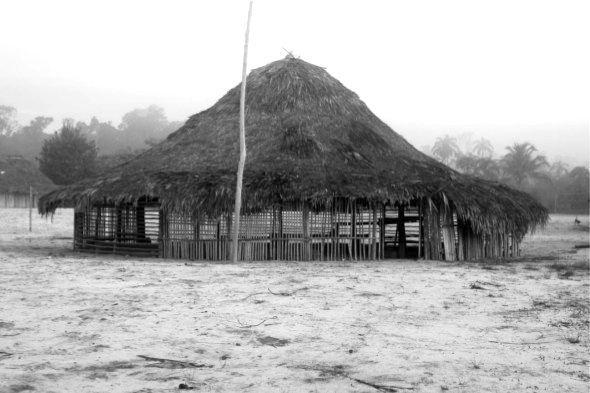
\includegraphics[width=\textwidth]{./img/027}
%\caption{Vista externa da maloca de \textit{Ta̗t"-Dëh} (foto: Danilo P. Ramos, 2011)}
%\end{figure}

Comparada às malocas de outras aldeias, a \textit{Ä̗g"-Mo̖y} de \textit{Ta̗t"-Dëh} pode ser
vista como uma das maiores e talvez a única construída a partir dos
princípios de arquitetura desana. A construção foi orientada por um
professor desano que assumiu turmas de ensino fundamental e passou a
morar na comunidade com sua família. Já as malocas das aldeias do
Cabari, Japú e Papuri, que visitei, têm dimensões mais modestas. Suas
estruturas se assemelham às das casas de moradia hup. É comum também
que, em muitas comunidades, a casa do dono, geralmente maior que as
demais, se constitua como espaço para a realização de festas de caxiri e
Dabucuris.

Seis ou quatro troncos firmes (acariquara)\footnote{\textit{w'ɨ̗h},Acariquara
  (\emph{geissospermum sericeum}). Cf. Ramirez (2006).} são fincados no
chão para constituir as fundações das casas. A essas colunas são
amarradas as ripas e os caibros\footnote{Usa"-se varas de paxiuba, mas
  também de \textit{tom tëg}, ``macucu'' (\emph{chrysobalaneaceae}), \textit{b'ä̖w
  tëg}, ``escorrega macaco'' (\emph{peltogyne paniculata}).} que darão
sustentação à cobertura de palhas de caranã que reveste o telhado. Em
\textit{Ta̗t"-Dëh}, a maior parte das casas possuem paredes laterais feitas com
casca de embaúba ou de embira, que criam a divisão entre um espaço
interno e externo. O piso é feito a partir do barro argiloso retirado da
beira dos igarapés. As casas fechadas possuem uma ou duas portas que se
abrem para dentro, feitas com varas e palhas de caranã. Jiraus feitos
com varas de paxiúba são instalados logo abaixo do telhado para guardar
caniços de pesca, arco e flechas, roupas, panelas, bacias, livros, entre
outros pertences dos moradores da casa.

Samuel descreve a maloca do alto da Serra da Iniciação como uma imensa
casa com 100 metros de área. Como em \textit{Ta̗t"-Dëh}, os ancestrais retiraram
seus instrumentos do local onde eram escondidos e caminharam para a
palhoça onde seus cunhados os esperavam. A imensa maloca constitui o
cenário hiperbólico para o encontro entre os habitantes da região, donos
animais, e aqueles que vinham de outras terras, do Lago de Leite. Os
forasteiros exibem suas flautas e dançam para seus cunhados, criando um
laço forte de reciprocidade. À luz da cerimônia de Dabucuri descrita, é
possível dizer que, ao longo da caminhada até a Serra da Iniciação, os
ancestrais assumem o lugar dos neófitos ao recolher e conhecer as
frutas, potências passíveis de gerar importantes relações de
reciprocidade. Pensando com Hugh"-Jones, ancestrais hup constituem"-se
como \textit{os de outras terras} e os animais como os \textit{donos da terra},
mas formam uma casa singular erigida por aqueles que dançam e conversam
dentro dela para criar as bases de um modo simétrico e complementar de
relação entre grupos afins.

Na maloca, ao tocar e exibir as flautas longe das mulheres, os
ancestrais hup assemelham"-se aos cunhados do \emph{sibling} \textit{Sokw'ä̗t},
``gente de outra terra'', que oferece frutos, respeita as interdições,
conversa pela \textit{linguagem de ocultar} e cria as condições para que os
descendentes sejam iniciados e se casem. Enquanto, na caça, o chamado
sedutor explicita o papel masculino do caçador e feminino da presa,
trazendo os frutos, os ancestrais hup ocupam uma posição masculina,
enquanto os Animais assumem posições femininas. A dança das flautas no
alto da serra parece apresentar os ancestrais como humanos plenos,
possuidores de objetos que são potências primordiais necessárias à
habitação e regeneração da vida nessas novas paragens. Dando as flautas
e constituindo um contexto próprio para que os ancestrais hup dancem, os
Animais apreendem os Hupd'äh como humanos e revelam"-se dotados de
perspectivas que contêm outras perspectivas.

Se em \textit{Ta̗t"-Dëh} é necessário que as \textit{gentes de outra terra} peçam
autorização aos donos e tornem"-se cunhados, o Dabucuri da Serra da
Menstruação não deixa de ser uma demonstração das habilidades dos
peregrinos para que possam, ao descer da serra e caminhar com suas
flautas, dispersar"-se e constituir seus próprios domínios (\textsc{m17})
(\textsc{m18})\index{27@\textsc{m}18\quad O \textit{caarpi} do Tamanduá}. Tomando as palavras de Lima, a dádiva das flautas na
Serra da Iniciação explicita que \textit{para os animais, a nossa alteridade
relativa com eles é humana, isto é, política}.\footnote{2005, p.\,215.}
\index{26@\textsc{m}17\quad Viagem com as flautas}

\section{Assentos marcados}\label{assentos-marcados}

Além da relação de afinidade entre Humanos e Animais, a assimetria
revela os Animais como os \textit{senhores da terra}, os primeiros a chegar e
a estabelecer os modos de ação que dão forma às interações durante os
Dabucuris. Entretanto, os recém"-chegados tiveram ainda que se sentar em
roda e beber o \textit{caarpi} oferecido pelo Tamanduá para revelar suas
habilidades xamânicas. Seguindo nossa conversa, Samuel contou a seguinte
narrativa:

\begin{quote}\index{27@\textsc{m}18\quad O \textit{caarpi} do Tamanduá}
\mito{18}{O \textit{caarpi} do Tamanduá}

O Tamanduá é o dono do \textit{caarpi}. \textit{Bɨ̗g we̗d no̗'o̗p, kapi̖', hu̖͂t}. Ele deu
comida a todos os animais, \textit{caarpi}, tabaco. Primeiro, deu para a Arara,
para o Papagaio e para o Periquito. Eles beberam e comeram a língua
(parte da). Não sabiam beber \textit{caarpi}. É por isso que falam hoje em dia.

A merda do tamanduá fede muito porque ele é o dono do \textit{caarpi}. Disse que
todos tinham bebido \textit{caarpi}. Daí, o \textit{Yawa̖ç}, Macaco"-Prego, escondeu o
rabo dele no banco e falou para os outros comerem o rabo. Disse que ele
já tinha comido. A Cotia, a Paca, a Cutivaia, a Anta, a Preguiça também.
O Uacari, o Porco, o Caititu, todos comeram o próprio rabo. Só o macaco
não comeu. Ele tinha escondido o dele. Tava enganando. Aí, o cunhado
perguntou onde estava o rabo deles. E eles já tinham comido. Ficaram sem
rabo.

Isso tudo aconteceu lá na Serra da Menstruação. Depois que tocaram, os
ancestrais hup sentaram nos bancos. Havia três tipos de banco: os
\textit{pud"-dë̖h käd}, ``bancos de leite'', os \textit{sãy käd}, ``bancos sãy'', e os
\textit{wahna̗w käd}, ``bancos de abiu''. Estavam usando cocar de penas de
mutum, arara e papagaio. Na cintura tinham pussangas: \textit{yo̗ k'e̖t} e \textit{hõ̗
pë̖' k'e̖t}. Tavam bebendo as cuias de \textit{caarpi} oferecidas pelo Tamanduá.
Eles ficavam alegres e cantavam \textit{kapiwaia}.\footnote{Caderno de campo,
27 de março de 2012). Uma versão desana dessa narrativa mítica é
  analisada por Buchillet (1983) em sua tese de doutorado.}
\end{quote}

\index{27@\textsc{m}18\quad O \textit{caarpi} do Tamanduá}
Entre um gole e outro de caxiri oferecido pelas mulheres, Samuel
contou"-me \textsc{m18} para explicitar o poder do Tamanduá como aquele
que dá o \textit{caarpi} aos Animais e aos Humanos. Dentro de sua grande maloca,
os Animais realizavam rodas de \textit{caarpi}. A bebida era oferecida aos demais
por esse mamífero que é um poderoso xamã. O oferecimento de \textit{caarpi}
diferencia os Animais entre aqueles que sabem e aqueles que não sabem
beber, ou seja, de acordo com suas habilidades. Aqueles que sabem beber
permanecem com seus corpos originais, mas aqueles que enlouquecem
intervêm sobre suas matérias corporais, automutilam"-se e veem"-se, ao
final da roda, desprovidos de suas longas línguas ou de seus longos
rabos. Como o pretendente a receber o cigarro do possível sogro
(\textsc{m18}), os forasteiros procuram demonstrar, através de seus
pertences, posturas e disposição para beber \textit{caarpi}, sua aptidão para a
prática do xamanismo e para a aliança.

\index{27@\textsc{m}18\quad O \textit{caarpi} do Tamanduá}
Aves como a Arara, o Papagaio e o Periquito comem partes de suas línguas
e, por isso, adquirem a capacidade de fala. É interessante reparar que
são justamente penas de papagaio e de arara que compõem os cocares dos
ancestrais (\textsc{m18}) e dos bebês no útero, estabelecendo uma
relação metonímica com essas \textit{aves que falam}. Como nas rodas de coca,
nos círculos de \textit{caarpi} as conversas entre os presentes e entre esses e
seus interlocutores cósmicos fazem da fala e da escuta importantes meios
sensoriais para a aquisição de saberes. Diferente das aves, o
Macaco"-Prego pode ser visto como um \textit{bom bebedor} já que não se
mutila. Mas sua extrema destreza xamânica faz dele um enganador capaz de
dissimular a autopredação para que os outros, embriagados, devorem seus
próprios rabos.

Sua ação o mantém como um animal do alto da floresta, diferente dos
animais de solo que, sem saber beber, se veem desprovidos de rabo e da
possibilidade de ocupar os níveis superiores da mata. Segundo Reid, os
Hupd'äh classificam a floresta verticalmente dividindo"-a em três níveis:
o ``chão'', \textit{su̗m}, o ``meio'', \textit{hak ten}, e o ``topo'', \textit{k'et d'öh}.
Como visto em \textsc{b7}\index{ah@\textsc{b}7\quad \textit{B'a' Bi'i̖d} \break Benzimento do Beiju}, essa separação tem importância tanto para a
caça, quanto para as práticas xamânicas, pois permite identificar os
animais de acordo com o nível habitado e com suas armas. Sentado num
banco, o macaco oculta seu rabo e, pela fala, mostra"-se capaz de agir
agressivamente contra seus companheiros. O banco oculta algo que será
perdido pelos maus bebedores de \textit{caarpi}, assim como a casa cercada oculta
as flautas Jurupari que seriam perdidas pelas mulheres, dada sua
incapacidade de tocá"-las (\textsc{m17}).\index{26@\textsc{m}17\quad Viagem com as flautas}

Durante a cerimônia do Jurupari, o flautim surge como uma figura ao
mesmo tempo cômica e agressiva. Neto dos grandes Jurupari, ele
\textit{brinca} com os rapazes agredindo"-os com o ramo de ingá. \textit{Rato} é o
nome desse instrumento"-criança, remetendo"-o a um espaço baixo da
floresta, a um nível inferior extremo, se comparado ao nível ocupado
pelo Macaco"-Prego. Como o macaco, sua ação intervém na matéria corporal
dos neófitos, endurecendo suas peles e transformando"-os em guerreiros. É
a partir de seus movimentos que a sequência oscila entre os momentos
descontraídos do caxiri, quando as flautas repousam no chão, e a dança
solene. Seus açoites criam a diferença entre os rapazes perseguidos e os
adultos oficiantes que gargalham à custa das reações dos novatos. Como o
flautim, o divertimento do Macaco"-Prego explicita a divisão entre \textit{os
que sabem} e \textit{os que não sabem} beber \textit{caarpi}, ou seja, revela a
diversidade de competências xamânicas a partir da corporalidade dos
presentes. Torna manifesto, igualmente, o enlouquecimento, já que os
\textit{maus bebedores} atentam contra si mesmos.\footnote{No caso,
  entretanto, os pássaros parecem aproximar"-se mais da posição do
  macaco"-prego (bom bebedor), que daquela dos animais que comeram o
  próprio rabo (maus bebedores), pois apesar de atentarem contra si,
  adquirem o domínio da fala.}

Seguindo com essa aproximação, as falas do Tamanduá: \textit{todos já
beberam} e \textit{onde está o rabo?} marcam transições na roda entre um
momento de comunhão e igualdade de oferecimento a todos, e outro em que
se ressalta a desigualdade de poderes xamânicos. Antes da saída, as
flautas fazem \textit{hihihi}, sinal para que os neófitos deixem a maloca. Já
os primeiros sopros e a melodia da entrada na maloca marcam movimentos
que evocam a presença de todos. De forma semelhante, ao sentarem"-se para
beber o \textit{caarpi} do Tamanduá, os ancestrais hup recebem o oferecimento de
modo equânime, mas diferenciam"-se de acordo com os bancos que ocupam.

\index{27@\textsc{m}18\quad O \textit{caarpi} do Tamanduá}
A narrativa \textsc{m18} delineia os traços de uma forma de interação
articulada à cerimônia de Jurupari, que se assemelha muito às rodas de
coca noturnas. O oferecimento é realizado por um dono que, como o dono
da coca, concentra a substância para oferecê"-la a seus agnatos Animais e
a seus afins Humanos hup. Como nos encontros noturnos, os participantes
permanecem sentados em bancos e conversam sob o efeito do alucinógeno.
Contam os senhores hup que antes de morar em \textit{Ta̗t"-Dëh}, sempre que se
realizava um Dabucuri, os mais velhos formavam rodas para fumar os
grandes cigarros cerimoniais, comer coca e beber \textit{caarpi}. Depois de
algumas cuias, os participantes animavam"-se e começavam a cantar os
\textit{kapiwaia}, os ``cantos do \textit{caarpi}''. Adornavam"-se, seguravam seus \textit{sö̖h},
``bastões'', e começavam a dançar na maloca. Os passos da dança, o som
dos bastões ocos chacoalhando as sementes, as visões de cores, formas e
seres criavam campos de percepção e ação através dos quais os
participantes viajavam pelo cosmos, interagiam com ancestrais e ouviam
encantamentos. Hoje, afastados da maloca em suas rodas nos dias de festa
de caxiri, vez ou outra um dos presentes cantarola um \textit{kapiwaia} e é
seguido por outros que, no entanto, não arriscam passos de dança.

As danças de \textit{kapiwaia} são lembradas em muitas das conversas dos
senhores nos encontros noturnos. Era geralmente em meio a Dabucuris de
iniciação dos rapazes, quando as flautas Jurupari eram tocadas, que se
formavam as rodas para o consumo conjunto do \textit{caarpi} e da coca.
Percebendo a nostalgia desses tempos em que os senhores bebiam \textit{caarpi} e
dançavam, perguntei muitas vezes o porquê da não realização do
\textit{kapiwaia} nos dias de hoje. Meus interlocutores respondiam: \textit{kapi̖' yu̗m
nɨ̗h, toho̗y ay}, ``não se planta mais caapi, acabou"-se''. O cultivo do
\textit{caarpi} era uma prática generalizada entre os senhores hup, mas
atualmente apenas os pajés mantêm plantações para o consumo próprio ou
para realizar encontros de iniciação xamânica.

Recebendo aqueles que pretendem beber o líquido em sua casa, geralmente
afastada da aldeia, o pajé prepara três tipos de \textit{caarpi}: \textit{ä̗g kapi̖'},
\textit{bi'i̖d kapi̖'} e \textit{ya̗m kapi̖'}, respectivamente ``\textit{caarpi} de beber'',
``\textit{caarpi} de benzer'' e ``\textit{caarpi} de cantar''. Ele sopra os potes de
\textit{caarpi} para que a substância fique mais forte, da mesma forma como o
dono do caxiri benze a bebida antes de oferecê"-la aos dançarinos no
Dabucuri. Seus visitantes, já abstêmios de relações sexuais há algum
tempo, permanecem dias deitados na rede alimentando"-se apenas com mingau
e beiju. Nesse período, todos bebem das cuias de \textit{caarpi} oferecidas pelo
anfitrião. Fumam e comem coca em grande quantidade. Dançam e cantam
\textit{kapiwaia}. Buscam, dessa forma, viajar para interagir com seres
diversos e encontrar seus antepassados. A partir desses deslocamentos,
os viajantes conhecem percursos e moradas, adquirem habilidades
xamânicas e ouvem encantamentos e mitos de seus interlocutores.

Ponciano, que participou de uma roda quando era jovem, contou"-me que ao
beber \textit{caarpi} soube que seria um ``xamã"-do"-banco'', \textit{kä̗d hup i͂h}, porque
seus ouvidos não permaneceram silenciosos durante o evento.\footnote{Numa
  festa de caxiri, em comemoração por nosso retorno da viagem às serras,
  o pajé Armando perguntou se eu gostaria de provar o \textit{caarpi}. Como
  manifestei interesse, ele me convidou para visitá"-lo em sua morada.
  Semanas depois, viajei com Samuel para a morada do pajé. Quando
  perguntei a ele se podia experimentar a bebida, ele disse que não me
  ofereceria mais o \textit{caarpi}, pois, conversando com parentes de \textit{Tõh
  Hayam}, ouviu que um antigo antropólogo enlouquecera ao tomar \textit{caarpi}.
  Segundo o pajé, embora pesquisadores bebam \textit{caarpi} com os Tuyuca ou
  Tukano, a força do \textit{caarpi} hup torna desaconselhável seu consumo por um
  branco.} Ouvia continuamente um ``chiado'', \textit{huhu̗y}. Esse barulho é
visto com uma sujeira que impede a concentração plena para ouvir e
aprender com os ancestrais e demais seres com quem o xamã interage
durante seus deslocamentos oníricos. Um som auricular mais intenso será
ouvido pelos \textit{bi'i̖d hup i͂h}, ``xamãs"-sopradores'', que serão capazes de
realizar apenas certos tipos de encantamentos, além de correr sérios
risco de enlouquecimento caso consumam tipos fortes de \textit{caarpi} como o
\textit{se͂he̖͂k kapi̖'}, ``\textit{caarpi} paricá'', e o \textit{hã̗wäg su̗' kapi̖'}, ``\textit{caarpi} de
pegar o sopro vital'', de consumo exclusivo dos pajés. Esses benzedores
têm no \textit{ä̗g caapi}, na coca e no tabaco substâncias cujo consumo os
permite sonhar, proteger e curar. Entretanto, não é necessário que um
senhor participe de uma cerimônia de \textit{caarpi} para tornar"-se um
xamã"-soprador. A participação nas rodas de coca, o encontro com
ancestrais em sonho, como no caso de Mandu (\textsc{s1})\index{ba@\textsc{s}1\quad O pai conta em sonho}, e a prática de
encantamentos vão, pouco a pouco, fazendo com que a pessoa se torne um
xamã"-soprador.\footnote{De um modo parecido, analisando a relação entre
  gritos e sujeira, Lévi"-Strauss (2004, p.\,360) aponta que ambos os
  termos surgem como mutuamente conversíveis dependendo da escolha do
  mito entre um código acústico, alimentar ou sexual. As restrições
  sexuais, alimentares e sonoras nas práticas xamânicas hup parecem
  explicitar também a conversibilidade mútua entre os termos barulho e
  sujeira.}

Como mencionado, a \textit{b'oto̗k wäg}, ``semente do ouvido'', localiza"-se
dentro da Casa"-da"-Audição (orelha) e desenvolve"-se principalmente
através das palavras que a fazem crescer à medida que a pessoa adquire
habilidades e saberes pelo aprendizado com pais e avós, pela interação
nas rodas de coca, pelas conversas oníricas e pelas viagens. Órgão
associado ao pensamento, a semente do ouvido está envolta por um algodão
branco semelhante ao que era encontrado pelos antigos no interior de
formigueiros e usado para acender fogo pela fricção de pedras. Trovões,
alimentos defumados e assados como carnes e peixes, barulhos, entre
outros fatores, sujam esse algodão e impedem que ao comer coca ou beber
\textit{caarpi} a pessoa cresça com as conversas e interações. Assim, os cuidados
com a alimentação do filho ajudam a manter a Casa"-da"-Audição o mais
limpa possível e contribuem para o desenvolvimento xamânico bem como a
narração de versões de mitos e encantamentos simplificadas e a
participação da criança em caminhadas, como a feita por Ponciano com seu
pai à Serra da Iniciação (\textsc{m17}). Essas ações preparam a pessoa
para que possa, mais tarde, ao participar da roda de \textit{caarpi}, ao beber a
água das nascentes ou ao ingerir a água do lago no topo da Serra Grande,
manter"-se em silêncio para ouvir da forma mais apurada possível os
ensinamentos dos ancestrais.\index{26@\textsc{m}17\quad Viagem com as flautas}

Dessa maneira, nas rodas de \textit{caarpi}, serão considerados \textit{säw}, ``pajés'',
somente aqueles que, ao beber, se encontrem em completo silêncio, sejam
habilidosos para viajar pelo cosmos, tenham marcantes experiências
visionárias e aprendam com os diversos interlocutores. A forma como um
pajé retira a doença do corpo da pessoa é levada em conta para
diferenciar os \textit{säw}. Aspergir água é uma ação realizada apenas por
alguns pajés que fazem com que o agente patogênico deixe o corpo
escorrendo com o líquido para o chão. Já os pajés que chupam extraem a
afecção maléfica pela sucção, retirando do corpo espinhos, pelos,
dentes, afecções de seres que tenham investido contra o doente. Com o
tempo, as viagens xamânicas tornam os pajés cada vez mais respeitados
tanto pelas curas e proteções que são capazes de executar, quanto pelos
feitiços e mortes que causam. A maestria no uso das variadas roupas
cósmicas, na realização de procedimentos de cura e proteção e na
capacidade para agredir e matar podem fazer do pajé um \textit{saka̗ka̗}, um xamã
extremamente poderoso e temido que concentra em si uma grande variedade
de técnicas, saberes e recursos.\footnote{Nos trabalhos de Hugh"-Jones
  (1996) e João Paulo Lima Barreto (2013) há referências aos pajés
  \textit{sakaka} tukano como sendo xamãs cujas habilidades advêm de suas
  roupas de cobra e da interação com seres dos rios e igarapés. Para os
  Hupd'äh de Vila Fátima, segundo Bruno Marques (comunicação pessoal),
  os pajés \textit{sakaka} são também aqueles cujas habilidades estão ligadas a
  roupas de cobra e às interações com os seres das Casas"-do"-Rio. Já no
  trabalho de Lolli (Lolli, 2010, p.\,70), \textit{sakaka} refere"-se à resina de
  uma árvore usada por caçadores para obterem mais presas.} Como
ressalta Hugh"-Jones,

\begin{quote}
Um segundo tipo de distinção, envolvendo graus relativos de saber e
poder, pode ser usado para ranquear os xamãs em uma hierarquia formal ou
informal. Nesses casos, o aumento de poder geralmente caminha lado a
lado com o aumento de ambivalência --- poderosos xamãs poderão ser
melhores na cura e também potencialmente mais perigosos que seus
semelhantes menos poderosos.\footnote{1996, p.\,36.}
\end{quote}

Se a sensibilidade auricular é um fator crucial para a diferenciação
entre os praticantes do xamanismo, a roda de consumo de \textit{caarpi},
coordenada pelo Tamanduá, diferencia os ancestrais hup de acordo com os
bancos que ocupam. Os \textit{sãy kä̖d} são os bancos de poder dos
xamãs"-do"-banco, enquanto os xamãs"-sopradores têm na madeira de abiu e,
portanto, no \textit{wahna̗w kä̖d}, ``banco de abiu'', uma substância fundamental
para curas e ações protetoras. Já os \textit{pud"-dë̖h kä̖d}, ``bancos de leite'',
constituem"-se como assentos comuns a todos os xamãs. De um modo
interessante, as categorias de praticantes do xamanismo hup e a relação
diacrítica estabelecida através dos bancos, índices das habilidades de
cada xamã, parecem assemelhar"-se ao modo como os Tukano atribuem aos
bancos e à postura sentada modos de ação marcados pela assimetria, pela
meditação calma que permite as viagens e a aquisição de saberes.

Como visto, nos encontros noturnos os anciões sentam"-se entre afins e
dividem"-se entre \textit{donos} e \textit{apanhadores}. As ações de preparo e
oferecimento diferenciam os presentes entre os \textit{donos da coca}, que
são também os \textit{donos da terra}. Já os \textit{apanhadores} são sempre
\textit{gentes de outras terras}, afins que raramente possuem plantações de
coca. Muitas vezes, na falta de bancos, os apanhadores sentam"-se no
chão, mas os donos sempre terão seus assentos, ainda que estes sejam
muito simples, como tocos de árvore ou tábuas de madeira. De modo sutil,
os assentos demarcam as posições hierárquicas na roda.

Entretanto, os anciões diferenciam"-se também de acordo com suas
habilidades, muitas vezes reveladas através das rodas de \textit{caarpi}. Nos
encontros noturnos, ao realizarem encantamentos, os bancos sobre os
quais se sentam os senhores hup, artefatos corporais e assentos
externos, surgem igualmente como bancos de leite, bancos de abiu e
bancos \textit{sãy}. Partilhando a coca e sentando"-se cada qual em seu banco,
os xamãs percebem"-se a partir da complementaridade e hierarquia de seus
poderes e habilidades múltiplas. Dessa forma, \textit{apanhadores} podem ser
grandes xamãs, como é o caso de Miguel, o que cria linhas transversais
às hierarquias estabelecidas com base no clã e na origem. Não é por
acaso que, ao contar uma narrativa mítica, o dono sempre interpela um
``cunhado'', \textit{yo̖h}, para confirmar e complementar suas palavras.
Movimentos e ações de determinados encantamentos, bem como curas e
proteções podem igualmente ser feitas de modo complementar, com o
beneficiário recebendo cigarros e/\,ou cuias com líquidos de xamãs afins.

Se as vozes e os rabos diferenciam os animais e suas capacidades por
meio de suas corporalidades, as roupas cósmicas, os ruídos e os bancos
xamânicos são igualmente índices diacríticos dos poderes dos senhores
hup. Retomando desenvolvimentos do capítulo \emph{Lagos de leite}, é possível ver a
importância que os xamãs hup têm para a regeneração da vida dos animai e
para a realização de seus constantes Dabucuri. Viajando para a
Casa"-dos"-Animais, os pajés oferecem tabaco e Espíritos humanos em troca
de presas. Batendo na pedra acústica, os xamãs"-do"-banco causavam o
estrondo que libertava as presas para a mata. Já o benzimento dos
alimentos realizado por xamãs"-sopradores e xamãs"-do"-banco destina os
espíritos dos animais para suas casas primordiais, possibilitando que
seus donos lhes restituam a vida, regenerando"-os. Segundo Århem, entre
Animais e Humanos haveria um pacto de reciprocidade cujo desrespeito
leva ao ataque predatório que causa doenças aos humanos.

Desse modo, se a relação entre Humanos e Animais se constitui por meio
do laço de afinidade e pelos Dabucuris, a atuação dos diferentes tipos
de xamã hup possibilita tanto a predação da caça quanto a regeneração da
vida. Enquanto a afinidade clânica é fundamental para que, através dos
casamentos, novos descendentes sejam gerados, a afinidade entre Humanos
hup e Animais permite que a caça seja como um casamento que estabelece
as condições para o convívio. No alto da Serra da Iniciação, o
oferecimento de \textit{caarpi} pelo Tamanduá diferencia os bebedores a partir de
suas habilidades xamânicas, corporalidades e pertences. As ações
complementares dos xamãs hup tornam"-se chave para que a afinidade dos
Humanos e Animais recrie a vida e possibilite as interações, danças e
cópulas dos Dabucuris. Já as flautas Jurupari marcam as diferenças entre
os \textit{donos da terra} e as \textit{gentes de outra terra}, dividem os
participantes entre neófitos e homens plenos e suscitam uma forma de
interação que, ao celebrar os laços de afinidade, fabrica o corpo dos
rapazes, produz as condições para boas alianças entre cunhados e
engendra um campo de percepção e ação através do qual ancestrais e
descendentes interagem a partir da continuidade entre seus corpos e
substâncias. A \textit{linguagem de ocultar} num tempo de caçadores refere"-se
à necessidade de honrar tal pacto de reciprocidade celebrado entre
Homens e Animais, do qual as mulheres foram excluídas. Não ver as
flautas poderosas que possuem nomes de animais talvez corresponda
paralelamente à não realização de caças pelas mulheres, formas de
afastá"-las da interação com as presas e com as potências dos animais.

\section{Caminhos de emaranhar}\label{caminhos-de-emaranhar}

O \textit{caarpi} e as flautas revelam"-se modos de mover"-se e interagir com
antepassados no fluxo de uma energia de contínuo que faz crescer xamãs e
neófitos a partir de sons, palavras e visões. Nesse sentido, minha
compreensão afasta"-se daquela de Reid (1979), que vê na dança das
flautas e no consumo de \textit{caarpi}, durante a cerimônia, modos de \textit{elevação
da alma} e de alternância entre vivos e mortos.

A análise do autor baseia"-se na analogia entre cipós que se estendem de
um plano cósmico a outro, conectando"-os, e a ingestão do \textit{caarpi}, bebida
preparada a partir de um cipó que, segundo o antropólogo, permitiria a
ascensão da alma à zona superior do cosmos onde se encontra a morada dos
ancestrais.\footnote{Ainda que tenha ouvido sobre cipós que ligam os
  planos"-casa cósmicos da mesma forma como os cipós conectam os níveis
  da floresta, não compartilho, a partir de meus dados, do princípio
  triádico, espécie de tríade estrutural que faz Reid (1979) ver
  analogias entre os modos de classificação do espaço florestal, do
  cosmos, dos mitos e dos encantamentos.} Entendo que, durante a
cerimônia das flautas, a dança e a ingestão de \textit{caarpi} fazem ancestrais e
descendentes coabitarem a maloca"-universo que se torna a paisagem da
criação, assim como o corpo passa a abrigar o Lago de Leite e as Casas
Ancestrais no nascimento e na agência xamânica. Certamente o \textit{caarpi}, o
caxiri e as flautas são elementos plenos de energia quente, uma potência
de crescimento e movimento, bem como de agressividade e força.
Entretanto, creio mais na energia de contínuo que atravessa ancestrais e
descendentes por meio dos gestos de dança, da coca, do sopro e do
\textit{caarpi}, do que na \textit{elevação das almas} e na alternância entre vivos e
mortos.

Do modo como compreendi, o \textit{caarpi} permite sonhar de um modo específico,
assim como o permitem o consumo noturno da coca e a ingestão de água nas
nascentes. Sob efeito dessas substâncias e a partir de posturas
corporais específicas (deitado na rede ou sentado no banco), os xamãs
deslocam"-se como pessoa"-sopro, fazendo surgir em si a paisagem da
criação ao mesmo tempo em que viajam para as moradas de outros seres. A
habilidade do ato de mover"-se por sonhos e encantamentos faz crescer os
xamãs, assim como o toque das flautas faz os jovens crescerem nos
saberes e fortalecerem"-se corporalmente. Pensando com Lima, posturas,
gestos e substâncias tornam a pessoa suscetível à perspectiva de Outrem,
permitindo que seja capaz de gerar um outro para si e dentro de si.

Surpreendido em minha segunda estada em campo pela melodia soturna das
flautas Jurupari, foi apenas após a partilha contínua da coca e dos
passos com meus interlocutores que comecei a entender melhor como a
interação dos rapazes com os velhos e ancestrais"-Jurupari faz com que
\textit{cresçam nos saberes} através de suas próprias ações e percepções na
partilha de experiências com seus preceptores e artefatos"-pessoa.
Trazidas para as aldeias e para as malocas no curso de viagens, as
flautas possuem longas histórias de interação com os antepassados que,
após a descida da Serra da Iniciação, separaram"-se para estabelecer suas
terras e suas moradas. Tocando as flautas, os rapazes aprendem a ligar
eventos e experiências próprias àquelas dos predecessores para retraçar
percursos.

No encontro da caça, predador e presa percebem"-se a partir de sua
história comum à luz das danças de Jurupari e das rodas de \textit{caarpi}
realizadas no topo da Serra da Iniciação. Soprando as flautas, os
rapazes conhecem os ancestrais partilhando sua companhia, assumem
posições num campo relacional que lhes permite partilhar experiências.
Nas rodas de coca, apanhadores e donos partilham igualmente esse
companheirismo que garante a agência xamânica complementar a partir das
habilidades singulares reveladas também pelas rodas de \textit{caarpi} e pelas
águas das serras.

Sentados nas rodas, seguindo pelos caminhos ou dançando com as flautas,
as pessoas são seus movimentos, \textit{crescem em saberes} à medida que
sopram, narram e se deslocam pelo mundo. Nos movimentos conjuntos, a
vida faz"-se um contínuo nascimento.

Explicitam"-se, assim, as relações entre esses diversos modos de ação,
formas de interação ritual que se constituem como campos de percepção e
ação entrelaçados por caminhos percorridos pelos viajantes hup em
contínuo processo de formação e transformação de si ao longo do mundo.
Os encontros noturnos e a cerimônia de Jurupari são o destino comum a
que todos chegam apenas para trilhar novos caminhos que os façam sentar
outras vezes em rodas e dançar novamente com as flautas em torno da
paisagem em perpétua criação.

%\begin{figure}
%\centering
%\includegraphics[width=\textwidth]{./img/029}
%\caption{Ponciano segue por um de seus caminhos (foto: Danilo P. Ramos, 2012)}
%\end{figure}

\chapter{Viagens a São Gabriel}\label{viagens}

\setlength{\epigraphwidth}{.60\textwidth}
\begin{epigraphs} 
\qitem{Toda vez que eu dou um passo\\
O mundo sai do lugar\\
E o mundo por ser redondo\\
Tem por destino embolar}{\textsc{siba}}
\end{epigraphs}

%\section{Rio abaixo}\label{rio-abaixo}

\section{O deslizar das canoas}\label{o-deslizar-das-canoas}

%\textsc{12 de abril de 2012}

No porto, a canoa grande de Américo nos esperava. O capitão, que fora
meu anfitrião durante a última estada em campo, navegaria comigo rio
abaixo até a comunidade tukano do Cunuri para que eu conseguisse
transportar minhas bagagens pelo igarapé seco e encontrasse Marcelino,
barqueiro e amigo desana, que me levaria de volta a São Gabriel. Samuel
animara"-se a viajar comigo à cidade para tentar expedir seus documentos
e dar entrada no pedido do bolsa"-família. Sentados lado a lado,
rumaríamos pelos rios grandes até esse estranho centro urbano que em
nada se assemelha à aldeia ou aos caminhos na mata. Logo cedo, visitei
algumas casas para dizer \textit{bay'ay}, ``adeus'', e fazer trocas finais. As
danças e o gosto do caxiri da festa de minha despedida do dia anterior
já manifestavam a saudade que começava a nascer.

Samuel pegou a pequena Graciela no colo, acenou para a esposa, vestiu a
mochila e seguiu comigo para a embarcação. Semanas depois, traria
histórias, algumas roupas para os filhos, documentos e a certeza da
aquisição do benefício social para os seus. A esposa levaria os filhos
para a roça e cuidaria da casa enquanto o marido estivesse longe. Os
filhos de Américo fizeram desenhos para mim e quiseram ir com a mãe
Isabel na canoa para despedirem"-se de mim no Cunuri. Todos instalados na
canoa, o capitão deu a partida na velha rabeta e zarpamos pelas águas
escuras do \textit{Ta̗t"-Dëh}, ziguezagueando pelas curvas, bancos de areia e
troncos caídos.

De repente, a canoa parou e ficamos de bubuia, sendo levados pela
correnteza. As crianças agarraram galhos das margens e Américo abriu a
cabeça do motor para analisar a situação e ver se dava \textit{jeito} na
rabeta. Na manhã anterior, sentamo"-nos ao redor dos motores de Américo e
de Rosalinho. Um deles estava com a pata quebrada, enquanto o outro
apresentava problemas no carburador. Engenhosamente, o capitão
substituiu o rabo de sua rabeta. Seu filho mais velho, Álvaro, passava a
chave inglesa, a chave de fenda, os pinos e dava a partida para testar o
funcionamento. Em torno das máquinas, formava"-se o contexto ideal para o
aprendizado da mecânica de navegação.

Os Hupd'äh foram descritos pela literatura etnológica como um povo \textit{sem
canoas} e desprovido de conhecimento sobre os grandes rios. Remando e
aceitando ser conduzido pelas rabetas, fui percebendo a íntima relação
que meus interlocutores têm com as canoas, com a pesca e com as águas.
\textit{Hoh"-të̖g hup nɨ̖h päpäd"-të̖g}, ``as canoas são os automóveis dos
Hupd'äh'', disse certa vez Samuel, rindo, numa festa de caxiri. Muitas
das canoas feitas a partir dos troncos escavados de \textit{hã̗'},
``louro'',\footnote{\textit{hã̗'}, ``louro'' \emph{(Ocotea tabacifolia)}, nome
  dado a várias espécies de árvores da terra firme utilizadas para a
  fabricação de canoas. Cf. Ramirez (2006).} foram fabricadas por
artesões tukano, de comunidades próximas, em troca de cestos de aturá ou
do trabalho de abertura de roças para suas esposas. Poucas embarcações
são novas, o que leva à necessidade de reparos constantes feitos com
breu. O uso das embarcações para a pesca intensificou"-se com a formação
da aldeia de \textit{Ta̗t"-Dëh} e com a permissão de pesca em partes do rio
Tiquié, dada pelos moradores do Cunuri.

%\begin{figure}
%\centering
%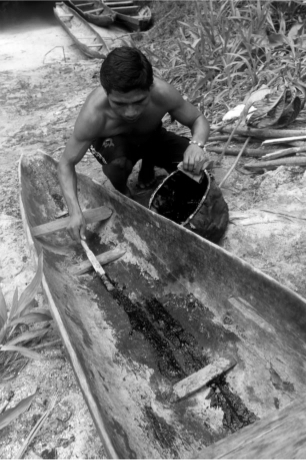
\includegraphics[width=\textwidth]{./img/030}
%\caption{Paulo repara a canoa com breu (foto: Danilo P. Ramos, 2012)}
%\end{figure}

Entretanto, as viagens para São Gabriel exigem embarcações maiores,
apropriadas para levar toda a família. Essas são compradas no comércio
local com o dinheiro de aposentadorias, bolsa"-família,
auxílios"-maternidade, salários de professores. As rabetas e a gasolina
tornaram"-se necessárias para os longos percursos pelos rios Tiquié,
Uaupés e Negro, que duram dias. Lonas de \textsc{pvc} azuis são estendidas nas
paradas para o repouso nos bancos de areia às margens dos rios quando
todos comem os peixes pescados e os beijus trazidos de casa. Por vezes,
alguma comunidade tukano pode se fazer de ancoradouro para o sono e para
a troca, mas é sempre preciso estar atento aos galões de combustível por
causa dos furtos recorrentes durante as paradas.

Quando chegamos à aldeia do Cunuri, Marcelino já nos esperava com a
grande \textit{ma̖yt hoh"-të̖g}, ``canoa de alumínio'', que, na região, recebe o
nome de voadeira. \textit{Quarentão pu̗b}, ``motor quarenta é forte'', exclamava
Samuel. Contou que o possante motor dos brancos é também o meio de
transporte com que \textit{Bisi̗w} foge logo que se apodera do \textit{hã̗wäg} das
pessoas. Ele escapa tão rápido que nenhum xamã consegue alcançá"-lo com
seus meios de transporte, roupas ou canoas movidas a remo e rabeta.
Assim, as máquinas e suas velocidades são percebidas como signos de
poder e riqueza por aqueles que levam muitos dias para chegar à cidade.
Alocamos nossas coisas na \textit{voadeira com quarentão}, despedimo"-nos de
Américo, Isabel e das crianças e seguimos cortando as águas, conduzidos
agora por Marcelino.

Mal começávamos nosso percurso, vimos, ao longe, alguém acenar para que
parássemos a voadeira. Um senhor tukano tinha morrido. O capitão da
comunidade nos pediu para levarmos o corpo até a aldeia de São Luis,
rio"-acima, para a família do falecido. Dois homens trouxeram o corpo
deitado em sua rede erguida por uma vara comprida. Um senhor hup, de
\textit{Pɨ̖̃g"-Dëh}, Nova Fundação, nos acompanharia, pois o morto era um dono
tukano com quem sua família mantinha uma história de trocas e afazeres.
Seu Avelino conhecia a irmã do falecido e, por isso, seria ele quem
entregaria a ela o corpo. Horas depois, tão logo aportamos, o homem hup
desceu, conversou com dois sobrinhos do defunto. Chorando e emitindo um
grito contínuo de dor, a irmã do dono tukano veio ao nosso encontro. Em
meio a sua tristeza, ela lamentava. Aproximou"-se do corpo, descobriu o
rosto, colocou a mão no peito do irmão e chorou sua perda. Os dois
sobrinhos ergueram o finado e todos subiram o barranco sem olhar para
trás. Sensibilizados e um pouco atordoados, retomamos nosso curso. O fim
da tarde aproximava"-se e, por isso, decidimos interromper nossa viagem
na aldeia tukano de Serra do Mucura. O senhor hup ficou para ajudar com
o enterro e depois seguir, caminhando, para sua aldeia.

Em Serra do Mucura, encontramos abrigo para nossa refeição noturna e
para o sono tranquilo. Somamos nosso macarrão à paca e beijus oferecidos
por nossos anfitriões. Marcelino e o capitão conversaram sobre política.
As eleições se aproximavam, Massa pensava em candidatar"-se como vereador
por seu partido. Comentaram sobre a corrupção da gestão do prefeito
tariano Padro Garcia e das promessas dos novos candidatos. Diante da
conversa em língua tukano, Samuel mantinha"-se quieto. Olhava para o chão
e, por vezes, comentava alguma coisa comigo. Sua atitude expressava o
respeito diante dos tukano, donos nesse universo que já não era mais
aquele de sua morada e de suas terras. Em língua hup, meu companheiro
contou"-me que próximo às casas onde estávamos havia rochas espalhadas
pelo morro que se erguia atrás da aldeia. (\textsc{m19})\index{28@\textsc{m}19} Antes de ser
morada de um ancestral tukano, o morro foi a \textit{Pa̖ç"-Moy},
Casa"-de"-Pedra, de um antepassado hup, \textit{S'ä̗bä̗y Hup i͂h}, o Lua.
Esse demiurgo possuía um \textit{me̖t"-bok}, ``tambor"-de"-pele"-de"-cutia''. Quando
tocava seu instrumento, as mulheres eram atraídas e vinham até ele para
se casar. Encantadas pelo som da percussão queriam a todo custo
deitar"-se em sua rede.

No dia seguinte, navegando as águas do rio Negro, Samuel avistou o morro
onde \textit{Wed B'ö̖'} habitou antigamente. Cutucou"-me e comentou que muitas
das histórias que eu tinha ouvido tinham se passado naquele lugar. Lá o
ancestral encontrou sua esposa, a Mulher Peixe. Lá ele provou a coca e o
tabaco pela primeira vez. Seu pai dissera que a Casa"-de"-Pedra desse
antepassado ainda possui as marcas de sua presença, assim como as serras
que visitamos, onde é possível encontrar, ainda hoje, os restos dos
potes de Semente de Tabaco. Guiado por Samuel, comecei a perceber as
paisagens que levam a São Gabriel, as interações com os Tukano e as
próprias embarcações que nos transportavam a partir de uma outra
perspectiva.

Seguindo Sahlins, as viagens a São Gabriel fazem circular pessoas,
ideias, objetos, coca, dinheiro nos deslocamentos entre polos culturais
estrangeiros e indígenas. De acordo com o autor, ao mesmo tempo em que
os viajantes hup adaptam"-se aos campos relacionais urbanos, mantêm
compromissos com suas famílias e comunidades gerando, assim, formas de
socialidade transculturais. Nas crônicas que seguem, procuro refletir um
pouco sobre como, através das viagens a São Gabriel, as pessoas hup
movimentam"-se pelos grandes rios, pelas ruas e pela escrita,
transformando modos de percepção e ação a partir das posições que
assumem em seus novos percursos orientados para a paisagem urbana.

\section{A coca de Marino}\label{a-coca-de-marino}

%\textsc{15 de abril de 2012}

A viagem a São Gabriel marcava a transição entre a convivência da aldeia
e o retorno vagaroso a minha cidade, São Paulo. Mas além de minha volta
e da busca de Samuel por seus documentos e benefícios sociais, nossa
incursão ao meio urbano tinha um outro objetivo importante, levar coca a
Marino para que ele se lembrasse de sua vida em \textit{Ta̗t"-Dëh} e retornasse
para casa com a família. Desde que seu pai, Henrique, falecera devido a
um tombo no banheiro mal equipado do posto de saúde da cidade, o xamã
passara a viver num bairro periférico na estrada que leva ao porto de
Cucuí.

Às vésperas de minha viagem de volta, Américo perguntou se eu levaria
coca para Marino. O irmão mais novo sabia que o outro estava com
saudades de comer coca. \textit{Pu͂'u̖͂k pa̖͂, noh k'ö̖d o̗to̗y}, ``se não tem coca a
boca chora'', foi a expressão que meu anfitrião utilizou para justificar
o pedido. Os riscos eram grandes. O exército andava revistando canoas,
na chegada a São Gabriel, por conta das punições ao comércio de carne de
caça e ao tráfico de cocaína. Entendendo a importância do pedido e a
saudade que Américo sentia de seu irmão, aceitei a missão que iria
cumprir com Samuel logo que chegasse à cidade. Por sorte, quando
atracamos no porto Queiroz havia apenas militares embarcando em um bongo
para Iauareté. As revistas estavam suspensas. Nossa carga valiosa estava
segura e, possivelmente, conseguiríamos cumprir nossa tarefa.

Ao encontrarmos Marino, deveríamos transmitir a ele também as ``palavras
do velho Firmiano'', \textit{Firmiano nɨ̖h ɨ̗d}. Sempre que conversava com
Américo, o preparador da coca dizia sentir falta de Marino nas rodas.
Para ele, como Henrique, Marino era um dos poucos que sabia conversar
bem nos encontros noturnos. Devido a alguns desentendimentos antigos,
Firmiano pouco falava nas rodas. Logo que terminava a preparação,
sentava"-se de costas para todos, voltando"-se para as cabeceiras. \textit{Hãwäg
hihu̗͂'u͂p tɨ̖h}, ``ele tem tristeza'', dizia Américo para explicar a
atitude de Firmiano. Dada sua afeição por Marino, fora ele quem nos
ajudara a preparar a grande quantidade de folhas de coca que colhemos
nos dias anteriores à partida.

Por cerca de três dias caminhamos para as roças de Marino todas as
manhãs. Seus pés de coca estavam cheios de mato, o que tornou nosso
trabalho mais difícil, pois foi preciso limpar a plantação. Colhíamos
com todo o cuidado e, com a ajuda de Samuel, logo enchemos um grande
saco com punhados de coca. Utilizamos o forno da casa de Américo para ar
as folhas e meu pilão para triturar bem a carne e os ossos do alimento
de origem. Deitando"-se folgadamente em sua rede enquanto eu pilava e
Samuel assava, Américo disse ser o \textit{dono da coca}, enquanto nós eramos
seus \textit{preparadores}. Rindo, o capitão lembrou"-se que antes, uma das
formas divertidas dos anciões se referirem à coca era chamá"-la de \textit{me̖t},
``cutia''. ``Quando tavam fazendo a coca, os velhos diziam: `Cadê a
cutia? Traz logo a carne pra gente assar. Pega o sal e a pimenta pra
preparar essa cutia!'", contou. A piada ficava mais engraçada quando
um participante pedia para ficar com o bucho, outro com o fígado, um
terceiro com os pés.

Essa \textit{muhu̗' ɨ̗d}, ``fala engraçada'', era também uma forma de \textit{yä̗d ɨ̗d},
``fala de ocultar'', pois, como caçavam muito, referir"-se à coca como
\textit{pu͂'u̖͂k} poderia causar diarreia aos comedores. Da mesma forma como o
Tamanduá é o dono do \textit{caarpi}, o Cutia é o dono da coca; por isso, ao
comer esse alimento é preciso explicitar as posições de presa da
cutia e da coca sendo devoradas pelos xamãs e caçadores hup. À predação da carne
e ossos do Velho Cobra sobrepõe"-se esse outro modo de ação, que faz do
encontro noturno um hilário consumo e distribuição da carne da cutia. O
sal da coca, imbaúba, transforma"-se no sal da carne e o tabaco em
pimenta, ambos para atenuar a presença de energia quente na presa
abatida. Predando a carne dos donos, os antigos predavam também a
posição de dono da coca, partilhando o alimento, o código culinário e
distribuindo a magnificação de suas vítimas no curso da fabricação
divertida de si enquanto \textit{comedores de coca}.

``Quando sonha com coca, que tá segurando um punhado de coca é que vai
caçar cutia. Pode pegar o terçado e o arco e flecha que vai matar'',
ensinou"-me Américo. Ele começava a se lembrar de como seu irmão Marino
era um bom caçador de cutias. Marino e seu pai, Herique, costumavam sair
logo cedo para a Serra da Cutivaia e, se tivessem sonhado, traziam
sempre uma cutia. Por conta de sua partida para São Gabriel, Marino
pediu que Samuel tomasse conta de seu cão de caça. Assando as folhas,
Samuel lamentou que o cachorro tivesse sido devorado por uma onça pouco
depois da mudança do dono para São Gabriel.

Em seu trabalho sobre o sistema hup de interpretação dos sonhos, Reid
afirma que a capacidade de traduzir símbolos oníricos pode ser vista
como uma fonte de informação sobre si mesmo e/\,ou sobre eventos latentes
no cosmos, imperceptíveis quando se está acordado. À luz de seu
comentário, no consumo da coca ou no sonho com cutia, a ação ritualizada
e a ação onírica situam as pessoas hup na posição de predadores. De modo
diferente, a viagem a São Gabriel faz Marino parar de comer coca e,
assim, \textit{cutia}. O \textit{esquecimento da aldeia}, a \textit{roça de coca cheia
de mato} e o \textit{cão devorado} vão situando o xamã na perigosa posição
de presa cuja condição humana precisa ser regenerada pela dádiva de seu
irmão menor, a coca.

Na manhã seguinte à nossa chegada, logo que acordamos pegamos de nossa
bagagem a lata com coca, tomamos um gole de café e seguimos para a vila
de Aparecida, no quilômetro 10 da estrada para Cucuí. Estávamos alojados no
escritório da \textsc{ssl} no centro de São Gabriel e, por isso, precisávamos de
uma lotação que nos levasse até lá. Conforme caminhávamos pelas ruas,
alguns rapazes riam do modo como Samuel usava suas meias altas calçando
uma sandália. Sem notar a burla, meu companheiro seguiu atento aos
carros, às lojas, ao movimento das pessoas. Da avenida principal,
levamos cerca de meia hora para chegar ao bairro distante. Casas de
madeira amontoavam"-se umas sobre as outras e formavam a vila de
Aparecida onde famílias tariano, tukano, desano, baniwa construíam suas
moradas. Perguntamos pelo xamã hup. Indicaram"-nos uma casa retirada,
mais para o fundo da vila.

Marino não estava. Era domingo e ele fora, acompanhado de dois vizinhos,
colher açaí na mata próxima. \textit{20 reais ayup balde}, ``20 reais o
balde'', comentou dona Mariquinha, esposa do xamã, segurando um pote com
chibé para oferecer"-nos. Durante a semana, seu marido trabalhava numa
pedreira, ganhando 20 reais por dia. Cuidava também do sítio de uma
funcionária do distrito de saúde, o que lhe dava uma renda adicional. As
filhas estudavam na escola do bairro. Não pensavam em voltar logo para
\textit{Ta̗t"-Dëh}, pois queriam que ambas terminassem os estudos. Moravam com um
cunhado do Cabari e com a família tariano de cunhados de um falecido
soldado hup, sobrinho de Marino, que se enforcara no ano anterior.
Entregamos o oferecimento de Américo a Mariquinha, transmitimos as
palavras de Firmiano e partimos. Na manhã seguinte, ela e seu marido
iriam à cidade para que eu os ajudasse a tirar documentos e a dar
entrada no pedido do bolsa"-família.

Na segunda"-feira, finalmente encontramo"-nos com o xamã que chegara ao
escritório acompanhado de sua esposa. Trazia nas mãos sua rede e a lata
com sua coca para que comêssemos juntos antes de irmos \textit{suk'e̖t yoho̗y},
``procurar os papéis''. O alimento da origem nos daria a força e a
serenidade necessárias para enfrentarmos as filas na polícia federal e
no cartório, para ignorar as burlas dos tukano, para caminhar por ruas
de asfalto tão distintas dos \textit{hup ti̖w}, ``caminhos de hup''. Antes de
sairmos, Marino viu as fotos que tiramos do alto da Serra Grande.
Comentou que no topo do morro há um pé de inajá. Se o viajante se banhar
nos lagos quando essa árvore está seca, seu corpo envelhecerá logo, mas
se ela estiver viva o corpo se regenerará. Os lagos de banhar eram
profundos antigamente e havia pés de coca às suas margens.

Tão distantes de \textit{Ta̗t"-Dëh}, em meio ao cenário urbano de São Gabriel,
posicionávamo"-nos numa roda de coca. Nossas conversas traziam à vida a
paisagem da criação cujas águas têm o poder tanto de degenerar quanto de
rejuvenescer. Como queria Américo, com o gosto da coca na boca, Marino
lembrava"-se de seu mundo vivido e de sua própria história naquelas
terras agora tão distantes. Entendo que ``comer coca antes de ir à
procura dos papéis'' revele"-se um \emph{esquecimento do esquecimento},
um ato de memória capaz de regenerar o xamã como um predador hup dos
encontros noturnos, que devora os donos da coca e partilha, com
caçadores (parentes hup da aldeia), a matéria e o poder do
inimigo"-outro, no caso funcionários e patrões, brancos e Tukano. Penso
haver uma reconstrução do sentido que permite a Marino e a Américo
estabelecer relações íntimas através do reforço mútuo dos planos
(aldeia, Serra Grande, São Gabriel) em que se exprimem seus
\emph{habitus} de pessoas hup em contínuo movimento ao longo do mundo.

%\section{Política}\label{poluxedtica}

\section{Carta para o prefeito
indígena}\label{carta-para-o-prefeito-induxedgena}\label{poluxedtica}

Eu havia acabado de retornar do trabalho de campo e escrevia os
relatórios a serem enviados às instituições locais na sede da Associação
Saúde Sem Limites (\textsc{ssl}) em São Gabriel da Cachoeira. Ricardo, um jovem
professor hup da comunidade de \textit{Yuyu̖-Dëh}, Barreira Alta, em sua
nova função de Assessor Pedagógico Indígena (\textsc{api}), estava na cidade para
entregar as listas de alunos das escolas hup do rio Tiquié e um abaixo
assinado à Câmara Municipal. Ele sentou"-se à mesa com o papel e o lápis
diante de si.\footnote{Até 2011, Ricardo exerceu a função de Assessor
  Pedagógico Indígena (\textsc{api}), responsável pelas escolas Hupd'äh do rio
  Tiquié. A função de \textsc{api} está vinculada ao fomento do controle social
  no âmbito do sistema escolar de São Gabriel da Cachoeira"-\textsc{am}.} Em
completo silêncio, escrevia uma carta ao presidente da câmara dos
vereadores. Seus olhos não desgrudavam do papel. Muitas palavras eram
arriscadas, mas logo a borracha desfazia suas marcas. A tensão parecia
tomar conta de seu corpo inteiro.

A apresentação do abaixo"-assinado para a construção de uma casa de apoio
para os Hupd'äh, na cidade, era muito importante. Sem nenhuma
interrupção no processo de escrita, depois de duas horas, Ricardo pediu
que eu lesse o rascunho que havia feito em seu caderno de anotações. Li
com atenção o pedido e apenas sugeri que fossem colocados a data e o
título do documento. Ele voltou para a mesa e começou a passar a limpo a
carta em uma folha de papel almaço com a caneta. Todo cuidado era pouco,
pois não queria errar e ter que escrever tudo de novo. Quando terminou,
pediu que eu a lesse novamente. Ricardo me olhava fixamente enquanto eu
relia a apresentação. Eu disse que estava ótima. Ele sorriu e seus
ombros soltaram"-se. Estava pronta a solicitação de casa de apoio que ele
apresentaria na manhã seguinte ao presidente da câmara.\footnote{Caderno de
campo, 2009.} Abaixo, transcrevo a carta redigida por Ricardo:

\begin{center}
\textit{Solicitação de casa de apoio para o povo Hupd'äh,\\
das comunidades dos rios Tiquié, Japu e Papuri}
\end{center}

Nós povos hupd'äh na região do rio Japu e papuri tanto do rio Tiquié. Solicitamos um casa de apoio, enquanto nós chegamos na cidade é difícil hospedar. Portanto nós queríamos essa casa poderia ser bem equipado tem banheiro masculino e feminino. Tem sala de cozinha, essa casa poderia ser duas quarto. Um quarto pode ser do rio Japu e Papuri, e outro quarto vai seria do Rio Tiquié. Nós queremos com mais ajuda a vocês com todas as instituições como: \textsc{funai}, Foirn, \textsc{semec}, e \textsc{prefeitura} Municipal. Como nós tambem professores indígenas, hupd'äh não tem como ficar no alojamento dos Tukano esses necessidades que nós tivemos na cidade. As vezes os Tukano que nos ralhava e sovina o alojamento, assim nós temos maior dificuldades que sentimos. Na hora da campanha o nosso prefeito indígenas \textsc{sr}. Pedro Garcia providenciou. Por esses motivo nós votamos o nosso prefeito indígenas para nos ajudarem a fazer.

\begin{flushright}
\textsc{são gabriel da cachoeira}\\
\textit{15 de maio de 2009}
\end{flushright}

A carta de solicitação acompanharia o abaixo assinado colhido nas
comunidades Hupd'äh de \textit{Yuyu̖-Dëh}, \textit{Ta̗t"-Dëh} e \textit{Pɨ̖͂g"-Dëh} durante o
período em que viajei, em maio de 2009, com uma equipe da \textsc{ssl},
realizando oficinas para projetos de alternativas econômicas. Os
professores hup haviam entregado um abaixo assinado, na câmara, com suas
assinaturas, mas o mesmo não foi suficiente para que o presidente
encaminhasse o projeto, pois este continha poucas assinaturas. A pedido
dos professores Pedro e Ricardo, nossa equipe conversara com os capitães
das outras aldeias e pedira que passassem o abaixo assinado. Todos os
capitães foram favoráveis ao pedido e escreveram, eles mesmos, os nomes
dos adultos da comunidade. Ao final, a lista era assinada pelo capitão,
atestando sua validade legal.

No documento acima, chama a atenção o modo como Ricardo seleciona os
argumentos e constrói a necessidade e importância da construção de uma
casa de apoio para os Hupd'äh. A solicitação é feita devido à
dificuldade de hospedagem. Em seguida, há a sugestão do modo como pode
ser construída a casa, incluindo suas divisões de dormitórios,
banheiros, cozinha. A solicitação torna"-se então um pedido de ajuda
feito a \textit{vocês com todas as instituições}. O relato da experiência dos
professores no alojamento tukano é evocado dando maior ênfase à
necessidade de auxílio. A campanha e a \textit{providência} do candidato
tukano eleito, Sr. Pedro Garcia,\footnote{O prefeito Pedro Garcia (\textsc{pt})
  foi eleito em 2008. Sua gestão durou até 2012 com sua derrota na
  tentativa de reeleição.} são lembradas no sentido de salientar o
apoio dado pelos Hupd'äh, com seus votos, e a importância da \textit{ajuda}
para que a construção se efetivasse de fato.

Chama a atenção o modo como Ricardo usa o sujeito \textit{nós} de diferentes
formas ao longo do documento. A princípio, \textit{nós} designa os \textit{povos
Hupd'äh} que solicitam a casa de apoio, havendo uma divisão entre
\textit{Hupd'äh do rio Japu e Papuri} e \textit{Hupd'äh do rio Tiquié}, onde mora
Ricardo. Essa divisão é retomada na distribuição dos quartos, um para o
rio Tiquié, outro para o rio Japu e Papuri. Em seguida, o \textit{nós},
\textit{povos hupd'äh}, ressurge oposto ao \textit{vocês} que engloba todas as
instituições detalhadas que ajudariam na construção. A intensificação da
dificuldade vivida pelos \textit{povos hupd'äh} emerge através do relato das
tentativas de hospedagem dos professores hup em São Gabriel, quando são
\textit{ralhados} (agredidos verbalmente) pelos Tukano que \textit{sovinam} o
alojamento, não permitindo, assim, a pousada dos professores hup. A
oposição entre o \textit{nós}, povos hupd'äh, e os \textit{outros}, tukano, revela
as dificuldades sentidas que justificariam a solicitação. Por fim, o
\textit{nós} mostra o apoio dado ao então prefeito, sr. Pedro Garcia, durante
as eleições. Ao mesmo tempo em que é ressaltada uma oposição entre
Hupd'äh e Tukano, parece haver uma unidade com o \textit{prefeito indígena},
um Tariano, na expectativa de que ele \textit{ajude a fazer}, assim como
\textit{providenciou} durante a campanha. Por fim, Pedro Garcia soma"-se ao
\textit{vocês} das instituições para ajudar a fazer a casa de apoio de que
tanto necessitam os povos hupd'äh.

Nesse sentido, pensando com Carneiro da Cunha, a elaboração do documento
situa"-se tanto no plano do ato quanto do discurso político, constituindo
sociedade, grupos e coletividades. O minucioso trabalho de fazer e
desfazer oposições entre \textit{nós}'' e \textit{outros} presente no documento pode
ser percebido como o processo de produção e discussão da autoridade para
representar os \textit{povos hupd'äh}. Isso permitiria a constituição da
autoridade do documento para representar um grupo indígena e para
realizar atos jurídicos em nome dessa autoridade.

Entre o rascunho e a finalização da carta, a leitura e aprovação de um
não indígena, antropólogo, seriam gestos importantes na busca pela
garantia de eficácia do documento enquanto instrumento dotado de
autoridade para representar o grupo indígena. Acredito que,
simultaneamente, o ato de escrever fosse também nutrindo Ricardo com os
atributos necessários para constituir"-se enquanto representante
legítimo. Ao mesmo tempo em que tece um elo entre as aldeias, o \textsc{api}
preserva a autonomia das mesmas na figura dos \textit{povos Hupd'äh}, e não
do povo Hupd'äh como poderia ser esperado. Além disso, ele cria uma
divisão arquitetônica entre os Hupd'äh do rio Tiquié e seu quarto, e os
Hupd'äh dos rios Japu e Papuri, e seu quarto comum. Algo que faz lembrar
as divisões presentes na grande maloca, onde os ancestrais hup tocaram
as flautas Jurupari para seus cunhados animais (\textsc{m18}), e as
divisões da casa celeste habitada pelo Trovão e seus cunhados, as Onças.
\index{27@\textsc{m}18\quad O \textit{caarpi} do Tamanduá}

Partindo da reflexão de Generre, o viajante"-escritor hup busca, a um só
tempo, exercer influência sobre o ambiente em que realiza seu ato
linguístico, mobilizar e concentrar a autoridade acumulada em sua pessoa
e exercer, assim, o poder da palavra. Seguindo Carneiro da Cunha,
percebe"-se haver, nos sentidos atribuídos à escrita, a confluência de
concepções de \textit{cultura com aspas} --- enquanto categoria manejada em
discursos para que reivindicações sejam atendidas --- e de \textit{cultura sem
aspas} --- enquanto ``esquemas interiorizados que organizam a percepção
das pessoas e que garantem certo grau de comunicação a grupos sociais''
. Nesse sentido, a concentração silenciosa por horas, o corrente
escrever e apagar, a elaboração do rascunho para submetê"-lo à aprovação
e o passar a limpo podem ser vistos como gestos de uma demonstração
performática de uma \textit{cultura com aspas}.\footnote{Carneiro da Cunha, 2009,
p.\,313.}

Visualizo essa \emph{performance} da escrita como um ``evento de
letramento'' (\emph{literacy}), uma ocasião em que a escrita se integra
à natureza das interações daquele que escreve e a seus processos de
interpretação. Na elaboração escrita das reivindicações dos \textit{povos
hupd'äh}, Ricardo elabora um discurso sobre a \textit{cultura com aspas} dos
Hupd'äh, marcada pela falta, pela discriminação e pela necessidade de
ajuda. Por um lado, os Tukano são aqueles que os discriminam e fazem com
que não possuam um alojamento próprio, por outro, apela"-se para o
prefeito tariano, um poderoso dono que, no entanto, encontra"-se em
débito com os Hupd'äh pelos votos recebidos. Sua ajuda, no final das
contas, trata"-se de uma forma de honrar uma relação de reciprocidade, um
circuito de dádivas semelhante ao do Dabucuri, iniciado pelos Hupd'äh ao
\textit{darem seus votos}.

\section{A política da
Cobra"-Canoa}\label{a-poluxedtica-da-cobra-canoa}

\begin{quote}\index{29@\textsc{m}20\quad A política da Cobra-Canoa}
\mito{20}{a política da cobra"-canoa}

No magistério, muitos Tukano contaram da história da Cobra"-Grande
dizendo que eles tinham saído primeiro. Política. Mas a verdade é que os
Hup tinham saído primeiro. Foi o Hupd'äh quem saiu primeiro da
Cobra"-Grande. Os Tukano dizem que foram eles, mas não é verdade, não.
Porque esses Hupd'äh, Dâw, eles foram timoneiros.

Saíram lá do Lago de Leite no Rio de Janeiro e vieram dar aqui. Primeiro
foram ali pra Ipanoré. Depois foram indo lá pra o Papuri, Iauareté, e
deixando os povos. Os Hupd'äh ficavam ali no rio Turi e daí foram
descendo, porque todos os povos vieram como peixes dentro da Cobra, mas
quando chegaram nos seus lugares eles já saíam e transformavam em gente.

Os Tukano falam muita coisa diferente do caminho da Cobra, por onde ela
foi primeiro, depois. É política, né. Falam que os Hupd'äh saíram
depois. Política.\footnote{Ricardo, 13 de maio de 2009.}
\end{quote}

Ricardo contou"-me essa narrativa enquanto jantávamos. Ele comia uma
quentinha que havia comprado por 5 reais. Para mim, comprou um espeto de
churrasco, que eu comia com gosto. O agrônomo Bruno Guimarães, professor
do \textsc{ifam},\footnote{Instituto Federal Amazonas (\textsc{ifam}).} que nos
acompanhava, apenas bebia suco. Conversávamos sobre o magistério
indígena\footnote{Segundo Azevedo (2003), na Região do Alto Rio Negro,
  as escolas tiveram início pela ação dos missionários salesianos no
  início do século \textsc{xx}. As escolas funcionavam com turmas multisseriadas,
  sendo os professores supervisionados pelas irmãs e pelo Instituto de
  Educação Rural do Amazonas (\textsc{iera}). A criação de escolas municipais nas
  terras indígenas torna"-se possível apenas em 1998, com a aprovação da
  lei do Sistema Municipal do Ensino. A partir daí, a prefeitura
  municipal realiza, através de magistérios, iniciativas de formação de
  professores indígenas de diversas etnias. São também ampliadas as
  séries de muitas escolas municipais.} e os Tukano. De repente, Ricardo
calou"-se, olhou para baixo. Ficou alguns segundos em silêncio e começou
a contar essa história. Da comida, seus olhos fixaram"-se em nós. Os
movimentos da Cobra"-Grande eram sinalizados por suas mãos que
ziguezagueavam pelo ar. A saída de cada povo era demonstrada por uma breve
pausa na narrativa e um leve movimento de erguer"-se e sentar"-se na
cadeira (Caderno de campo, 2009).

Contada dias antes do evento em que Ricardo redigiu a carta de
solicitação, a história surge em meio a uma conversa sobre o magistério
indígena, quando os Tukano narram a viagem na Cobra"-Canoa, afirmando sua
saída anterior. Essa forma tukano de contar é tida como sinônimo de
\textit{política}. Para além dessa forma de contar estaria a \textit{verdade} no
fato de os Hupd'äh terem saído primeiro da Cobra"-Grande. A explicação
mostra os Hupd'äh e os Dâw como timoneiros, aqueles que conduziram a
Cobra em sua jornada do Lago de Leite, no Rio de Janeiro, até a
cachoeira de Ipanoré. Na unidade interior da Cobra"-Grande, todos os
povos eram peixes que, ao sair, chegavam a seus lugares e
transformavam"-se em gente. O modo diferente de narrar dos Tukano é visto
como \textit{política} e \textit{não verdade}, diferente da fala Hupd'äh, cuja
verdade seria manifestada pelo modo de relatar o percurso da cobra, pela
condução da embarcação e pela saída anterior. Afinal, foram eles os
timoneiros.

Nessa narrativa, opõem"-se modos de narrar que revelam a oposição entre
Hupd'äh e Tukano em termos políticos de verdade e não verdade. O
magistério e a Cobra"-Grande são totalidades que contêm a multiplicidade
dos povos. No magistério, os Tukano contam de forma diferente sobre o
percurso da Cobra. Dizem que saíram primeiro. Fora do magistério, o Hup
Ricardo conta a dois não indígenas a história, revelando o caminho
verdadeiro e a saída anterior dos Hupd'äh. Como aponta Hugh"-Jones,

\begin{quote}
A mito"-história do Alto Rio Negro é uma história política em um duplo
sentido. Por um lado, fazendo referência a estrangeiros, as narrativas
de todos os grupos da região refletem uma longa história de resistência
à dominação externa e servem para legitimar reivindicações indígenas
pelo território. Por outro lado, histórias particulares servem também
para legitimar reivindicações pelo território, bem como status de um
grupo particular em face aos demais.\footnote{2012, p.\,163.}
\end{quote}

Creio que a \textit{política} à qual se refere Ricardo tenha a ver com essa
busca por legitimar territórios e \emph{status} por meio da
mito"-história da região. Segundo Athias, na visão de mundo dos Tukano,
os Hupd'äh habitam as florestas, e não as margens dos rios, não possuem
moradas fixas nem ornamentos, não praticam a exogamia linguística e não
são horticultores. Contrastivamente, do ponto de vista tukano, os
Hupd'äh são marcados por aspectos negativos e não humanos que os levam a
comportamentos incestuosos, animalescos e selvagens. Já do ponto de
vista Hupd'äh, como visto anteriormente, é preciso cuidado e atenção ao
interagir com os Tukano, dada a presença excessiva de energia quente e
agressividade em seus corpos. Atitudes arbitrárias, a altivez e mando,
inabilidade para caminhar pela mata ou para caçar, por exemplo, são
aspectos que aderem à identidade atribuída pelos Hupd'äh aos Tukano.
Apesar de violentos e agressivos, os Tukano, restritos ao universo
ribeirinho, desconhecem saberes fundamentais imanentes às paisagens e
ouvidos nas interações com animais e espíritos que habitam as moradas ao
longo das trilhas. Desconhecem as narrativas \textit{verdadeiras} sobre a
origem dos povos da região, chegaram depois às terras do Uaupés e foram
impelidos, pelos feitiços praticados contra eles, a deixar suas aldeias
e migrar para São Gabriel.\footnote{Em \textit{Ta̗t"-Dëh}, em discursos feitos
  antes de uma festa de caxiri, algumas lideranças hup manifestaram ter
  pena das famílias tukano por terem sido vítimas de tantos feitiços que
  acabaram sendo forçadas a deixar suas moradas e tentar a vida em São
  Gabriel. Os objetivos das viagens dos Hupd'äh a São Gabriel visavam a
  obtenção da maior quantidade possível de recursos, bens e benefícios
  para serem trazidos às aldeias. Pensando com Sahlins (1997), parece
  haver a intenção para a atuação em contextos transculturais que, tendo
  como referência sempre a aldeia hup, busca englobar poderes, objetos e
  signos para proteger a todos da ação xamânica agressiva que faz com
  que as pessoas tenham que abandonar suas casas e parentes.} São,
assim, vistos como pessoas fracas por não dominarem a agressividade que
degenera no \textit{autoritarismo} com que tratam os Hupd'äh.

Na carta, o \textit{ralhar} e \textit{sovinar} dos Tukano, atitudes antissociais
reprovadas pela socialidade hup, reforçam uma oposição entre nós, povos
Hupd'äh, e outros, Tukano. Essas atitudes atestam a dificuldade para a
hospedagem e justificam a unidade com o \textit{prefeito indígena}, Tariano,
e com \textit{vocês}, todas as instituições, na ajuda para fazer a casa de
apoio. Na narrativa acima, a fala política dos Tukano opõe"-se à fala
verdadeira dos Hupd'äh, havendo, no caso, certa superioridade dos
segundos por terem \textit{a verdade}, já que foram os timoneiros da
Cobra"-Grande que saíram primeiro e, assim, povoaram a terra
anteriormente. Os gestos de ondular os braços, de erguer"-se levemente a
cada saída de um povo da Cobra"-Grande mostram o saber e a verdade do que
se fala, já que o narrador \textit{sap bë'ëy}, ``gesticula'', demonstrando a
partir dos movimentos feitos com o próprio corpo o saber sobre o que
fala.

No documento escrito, a oposição entre Tukano e Hupd'äh embasa certo
sentido de uma \textit{cultura com aspas}, em que os primeiros são superiores
aos segundos. Salienta"-se também as dificuldades sentidas pelos Hupd'äh
e a necessidade de serem ajudados. A anterioridade tukano pode ser
percebida pelo fato de terem alojamento antes dos Hupd'äh, de serem
capazes de \textit{ralhar} e \textit{sovinar}. No magistério, a narrativa oral dos
Tukano, sua política, procura mostrar uma origem comum onde eles,
Tukano, seriam superiores. Essa fala, tida pelo narrador como sinônimo
de inverdade, transforma"-se, na carta, na possibilidade de construção da
casa de apoio. Como afirma Carneiro da Cunha,

\begin{quote}
Para atingir seus objetivos, porém, os povos indígenas precisam se
conformar às expectativas dominantes em vez de contestá"-las. Precisam
operar com conhecimentos e com a cultura tais como são entendidos por
outros povos, e enfrentar as contradições que isso venha a gerar.\footnote{Carneiro da Cunha, 2009, p.\,330.}
\end{quote}

Como afirma Andrello ao analisar uma narrativa tukano, ``no presente,
não se trata de se apropriar da perspectiva de outrem, mas de afirmar a
sua própria''.\footnote{2006, p.\,421.} Movimentando"-se entre o oral e o escrito,
Ricardo mescla de diferentes formas concepções de ``cultura'' e cultura.
Parte de um campo de interações marcado pelas relações com os Tukano em
meio ao convívio dos afazeres em aldeias e roças ribeirinhas, às festas
de Dabucuri e de caxiri interétnicas, à passagem pelas comunidades
tukano durante as viagens à cidade, e à participação conjunta nos
magistérios. Em sua carta, a ``cultura'' surge no discurso escrito pela
caracterização dos Hupd'äh como inferiores. No discurso oral, a cultura,
sem aspas, delineia os Hupd'äh como superiores pela verdade,
anterioridade e saber. Em diferentes situações, tenho observado a
inversão que marca a diferença entre esses dois discursos. Quer no modo
de manifestar"-se diante da presença dos Tukano ou em sua ausência, quer
na interação com equipes de saúde, pastores evangélicos, representantes
da \textsc{funai} ou lideranças, essa inversão, de acordo com o contexto
relacional e a posição assumida, permite, a meu ver, que suas
reivindicações sejam atendidas.

\section{Livro de Encantamentos e\break círculos de
cachaça}\label{livro-de-encantamentos-e-cuxedrculos-de-cachauxe7a}

Sentado ao meu lado numa roda de coca, Jovino lembrou"-se de quando a
polícia federal chegou às comunidades na década de 1980. Os policiais
aproximavam"-se, mandavam chamar aqueles que tivessem plantações de coca.
Os anciões aproximavam"-se e eram acompanhados até suas roças de coca.
Lá, furiosos, os brancos arrancavam os pés de coca. Xingavam e
humilhavam os senhores, enquanto faziam montes com as plantas. Atônitos,
os velhos viam suas plantações serem queimadas diante de seus olhos, sem
poder fazer nada. ``É por isso que os Tukano e algumas aldeias hup mais
próximas do Tiquié não têm mais muita coca, os velhos não conversam mais
e não têm benzedores bons'', disse Jovino, para reforçar a importância
de escrevermos conjuntamente um Livro de Encantamentos hup, como aqueles
que algumas comunidades tukano estavam fazendo com a ajuda de
pesquisadores. \textit{Surara tä̗w pu̗b}, ``os milicos são violentos'', era como
os xamãs referiam"-se aos oficiais quando recontavam para mim a história
da queima da coca que, reversamente, manifestava a importância que
atribuíam ao meu trabalho. Poucas plantações hup foram atingidas pela
truculência dos policiais, mas, como no caso do Jurupari, roças e
encontros noturnos passaram a ser motivo de reserva.

A urgência da preparação do livro devia"-se também à dificuldade da
geração atual de adultos em adquirir as habilidades necessárias para a
realização de encantamentos. Como visto anteriormente, a pessoa é
preparada desde muito cedo para a participação nas rodas de coca e para
o aprendizado das palavras, modos de interação e mobilidade xamânica. Ao
longo das últimas décadas, a dificuldade na obtenção de alimentos, a
permanência de algumas crianças nos internatos salesianos, os períodos
de trabalho no garimpo e as viagens a São Gabriel tornaram difícil aos
pais a preparação de seus filhos para as práticas xamânicas. Ao ouvirem
encantamentos, seus pensamentos se espalham, ao invés de seguirem direto
(movimento retilíneo). As Casas"-da"-Audição possuem constantes ruídos,
resultado da dieta ruim e da exposição à música e sons de motores e
máquinas dos brancos. Ao contrário, a habilidade de leitura e escrita
adquirida pelos filhos adultos com os estudos nas escolas salesianas
surpreendia os xamãs, sendo vista como um poder fundamental de interação
com os brancos, o qual poderia ser utilizado para contribuir com o
aprendizado. Pensando com Carneiro da Cunha, creio que essa articulação
entre viagens cósmicas, atos de fala (encantamentos soprados) e palavras
escritas revele o processo como uma tradução xamânica é ``capaz de
apreender os pontos de ressonância, de fazer com que a \emph{intentio}
em uma língua reverbere em outra'' (1998, p.\,13).

Logo que as primeiras transcrições ficavam prontas, os escritos eram
levados às rodas. De modo muito atento, os senhores acompanhavam a
leitura em voz alta, realizada por mim ou pelo neófito que havia me
ajudado a transcrever e traduzir os encantamentos narrados pelos xamãs e
registrados em meu gravador. Nessas audições, as versões eram comentadas
e complementadas, pois os textos diziam respeito apenas a movimentos
elementares do conjunto de ações que precisavam ser realizadas pelo
benzedor.\footnote{As exegeses analisadas nessa tese dizem respeito a
  esses textos mais elementares.} Os textos passaram a ser veículos de
mediação para as conversas entre os mais jovens e os comedores de coca.
Alguns, como Samuel, dedicaram"-se durante longo tempo à leitura e
conversa com os mais velhos sobre encantamentos importantes, para
proteger e curar suas famílias. A participação de Samuel na viagem à
Serra Grande partiu desse interesse em caminhar pelos lugares aos quais
seu pai se referia nas histórias e nos encantamentos que lhe ensinava.
As linhas de nossa escrita buscavam não aquilo que Ingold denomina
linearização, uma cadeia de ligações ponto a ponto que exclui a vida nas
conexões do gesto, mas sim descrever os movimentos dos viajantes ao
longo do mundo para que as linhas da escrita se movessem como os
próprios xamãs.

Desse modo, o processo de preparação do livro estabeleceu um campo mútuo
de interação em torno de palavras e escrituras que foi aos poucos
gerando transformações no modo de circulação de saberes e habilidades
das rodas de coca e dos caminhos. Apesar de não haver mais a necessidade
de \textit{yä̗d}, ``ocultar'', tantas palavras e tantos sentidos dos
encantamentos, os senhores hup decidiram que seria importante que o
livro resultante de nosso trabalho fosse um exemplar único, que deveria
ser mantido apenas nas mãos dos participantes das rodas, para que
crianças, mulheres e pessoas de outras aldeias hup não tivessem acesso.
Se o poder da escrita contribuía para o aprendizado dos homens, o
contato indevido com esses saberes poderia ameaçar a saúde das mulheres
e mesmo fortalecer a ação de feiticeiros inimigos. Em minha tese, eu
poderia utilizar as versões traduzidas das exegeses de encantamentos,
mas não aquelas em língua hup. A tradução para a língua dos brancos e a
escrita geram um enfraquecimento das palavras e ações dos encantamentos,
o que ajuda a \textit{ocultar} os sentidos e diminuir os riscos do uso
agressivo dos saberes ou do impacto prejudicial das ações.

Num sentido inverso, nesse gradiente de poder das palavras, acompanhei o
uso cada vez mais frequente da língua portuguesa nas festas de caxiri,
quando moradores retornavam de São Gabriel com engradados de cachaça.
Regadas às doses de Velho Barreiro, rodas de consumo da bebida
formavam"-se com o oferecimento feito pelo viajante recém"-chegado.
Oferecer a cachaça é uma maneira de expressar o sentimento de que, em
sua incursão à cidade, a pessoa não se esqueceu dos parentes e de sua
vida em \textit{Ta̗t"-Dëh}. À medida do efeito embriagante do álcool, a energia
quente e agressiva dos brancos começa a tomar conta dos corpos e
expressões dos bebedores. \textit{Seu merda}, \textit{filho da puta},\textit{vai tomar
no cu}, \textit{burro} são ofensas proferidas por alguns dos participantes
das rodas que começam a se desentender com parentes próximos. Nas rodas
de coca, consumido algumas doses de cachaça, os anciões observam o
comportamento e a violência que toma conta de alguns dos homens e
rapazes.

Como na situação da queima das roças de coca, os xingamentos são vistos
como uma \textit{tä̗w ɨ̗d}, uma ``fala furiosa'' que manifesta potências
destrutivas e, ao mesmo tempo, a força dos brancos em si. Beber a
cachaça e falar como os brancos revelam uma complexa mimese através da
qual os bebedores situam"-se num campo de interação com esses Outros, o
que torna possível o alinhamento de suas atenções, gestos e falas a
partir da observação do comportamento violento desses Outros. Se as
roupas"-cósmicas dotam os xamãs das habilidades das onças, mulher"-fera e
\textit{Bisi̗w}, creio que as rodas de cachaça e os xingamentos em português
deflagrem um processo reflexivo de apreensão de potências arbitrárias e
violentas que marcam as viagens e as interações na cidade a partir de
alinhamentos da atenção proporcionados pela cachaça. Num outro sentido,
a escrita parece ser um modo de ação que, articulado às rodas de coca,
abre a possibilidade de atenuar efeitos negativos da interação com os
brancos em suas escolas, igrejas e cidades. As \textit{falas furiosas} e a
escrita parecem ser modos de colocar"-se em perspectiva e assumir o olhar
e a agência de outrem.

Numa roda de coca de 2011, conversei com João sobre as casas cósmicas
que são visitadas pelos xamãs durante suas incursões ao universo
celeste. O benzedor contou que uma das moradas fundamentais para a
viagem do xamã vem a ser a \textit{Sib'i̖-Moy}, a Casa"-da"-Cachaça. Suas
paredes de tijolo, suas telhas de barro e suas janelas de vidro dão a
ela a aparência de uma construção de alvenaria. Chegando à
Casa"-da"-Cachaça, o benzedor precisa encontrar"-se com os xamãs, \textit{bi'i̖d
hupd'äh}, e ``feiticeiros'', \textit{pë̗' hupd'äh}, ``gentes"-da"-doença'', que lá
habitam. Atualmente, essa morada abriga dentro dela a Casa"-da"-coca, a
Casa"-do"-Tabaco, a Casa"-do"-Caxiri, a Casa"-da"-Pimenta e a Casa"-da"-Farinha,
todas essas substâncias fundamentais para o crescimento e alimentação.
Essas moradas são, assim, englobadas pela grande Casa"-da"-Cachaça,
espécie de campo transcultural a partir do qual os xamãs buscam se
posicionar para observar de todos os ângulos e empreender suas
tentativas de totalização dos pontos de vista singulares e irredutíveis
que se encontram em contínua ressonância. Partilhando os alimentos com
os xamãs dessas moradas e assumindo suas perspectivas, o viajante
adquire habilidades e saberes que lhe permitem maior êxito nas ações
protetivas ou agressivas.

A Casa"-da"-Cachaça edifica"-se como uma estrutura que contém outras
moradas, revelando"-se um sintético campo relacional branco que envolve
outros planos de atuação e percepção proporcionados pelas demais
substâncias. Enquanto as práticas eméticas pela ingestão de águas nas
nascentes dos morros mostram"-se formas de relacionar"-se, como ocorre com
as potências da morada do Trovão e das Onças que dominam as
armas"-de"-fogo e se enfurecem quando bebem cachaça, o consumo do
destilado e a viagem à Casa"-da"-Cachaça parecem fazer o xamã assumir a
perspectiva dos brancos alinhando sua atenção e ação para um modo de
abdução da agressividade e força desses Outros num sentido próximo ao
das rodas de cachaça na chegada dos viajantes.

%\begin{figure}
%\centering
%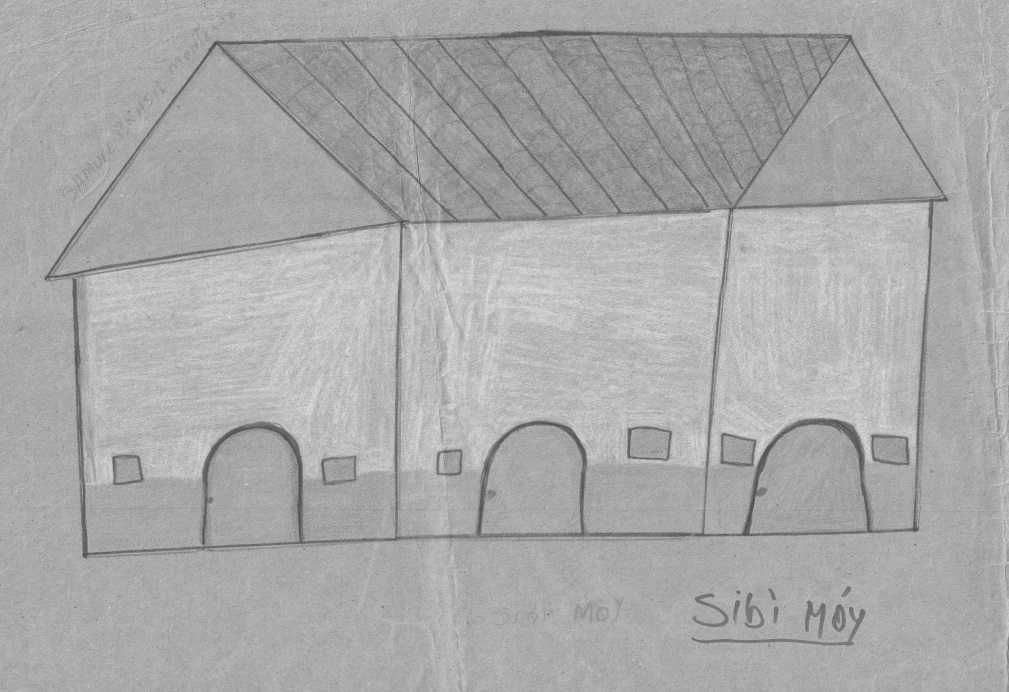
\includegraphics[width=\textwidth]{./img/031}
%\caption{Casa"-da"-Cachaça (Desenho de Samuel Brasil Monteiro, /M'e̖h Sɨh/)}
%\end{figure}

Nos últimos anos, têm se tornado cada vez mais frequentes as incursões
de senhores hup a São Gabriel. Deslocam"-se conduzidos pelos filhos para
o centro urbano em busca do acesso a seus direitos de aposentadoria.
Devido à morosidade, burocracia e discriminação locais, são necessárias
inúmeras viagens e períodos longos de permanência longe da aldeia. Sem
alojamento ou local seguro para a estada, os senhores permanecem
acampados, nas pedras de Parauari, em barracas, enquanto seus filhos
transitam pelas ruas da cidade solicitando a expedição de documentos e
dando entrada no pedido dos benefícios. Quando sua presença é exigida,
os senhores deixam o acampamento e são levados para se apresentarem no
cartório, banco, \textsc{funai}, etc.

As rodas de cachaça são comuns nesses períodos quando os viajantes bebem
com parentes de outras comunidades e com pessoas de outras etnias em São
Gabriel. A embriaguez que marca a experiência da cidade é contada nos
encontros noturnos da volta em meio às impressões sobre a música, a
comida, a polícia, os automóveis e demais aspectos que tenham chamado a
atenção dos anciões. Novamente em seus lugares nas rodas, os
recém"-chegados falam de suas bocas que choraram a falta da coca, dos
roubos dos quais foram vítimas e de desentendimentos que seus filhos
tiveram com pessoas de outras etnias, principalmente tukano. O sabor da
coca e a ardência da cachaça acompanham sorrisos e piadas que traduzem a
sensação de terem vencido perigos e desafios nas aventuras pela cidade,
uma imensa, fascinante e terrível Casa"-da"-Cachaça.

Conviver com os brancos, viajar para as cidades, estudar nas escolas
enfraquecem o corpo para a aquisição de habilidades xamânicas, ao mesmo
tempo em que a escrita em língua hup e a tradução para o português
enfraquecem a força das palavras dos encantamentos. Inversamente, as
viagens à Casa"-da"-Cachaça, à cidade de São Gabriel, o consumo de cachaça
e o aprendizado da escrita colocam"-se como modos de ação que levam à
abdução de poderes que fortalecem os xamãs, asseguram o aprendizado dos
adultos e garantem que sempre que estejam em São Gabriel, como nas
visitas aos planos"-cósmicos de seres perigosos do universo, os viajantes
lembrem"-se de seus parentes e voltem para suas comunidades. No curso das
viagens a São Gabriel, a ressonância de pontos de vista torna"-se
possível pelo consumo da cachaça e pela escrita, agências essas que
revelam poderosas relações analógicas que tanto reestruturam fenômenos
quanto conferem significado. A cachaça e a escrita demonstram, na
aldeia, aquilo que a \emph{coca de Marino} e a \emph{carta ao prefeito
indígena} procuravam revelar na cidade, ou seja, a importância da
percepção de si como Hupd'äh interagindo com brancos, Tukano, para
adquirir habilidades e substâncias outras, abduzir poderes que os
permitam se posicionar em campos de percepção e ação englobantes para
apreender pontos de vista em ressonância e retornar, proteger e curar os
seus.

\section{Saudades de Henrique}\label{saudades-de-henrique}

Em 2009, sem saber ainda a melhor forma de despedir"-me para um longo
período de afastamento, abracei o senhor Henrique. Sofrendo com uma
gripe aguda, ele passava agora seus dias deitado em sua rede reanimando
o fogo que mantinha seu corpo aquecido. Não ia mais às rodas comer sua
coca e também não era mais conduzido pelas mãos de seus netos durante as
perambulações que fazia pelas casas de seus muitos \textit{te̖͂h däh},
``filhos''. Dei a ele minha rede e disse, com as poucas palavras hup que
sabia, que no próximo ano nos reencontraríamos. Henrique olhou para mim
e disse que não estaria mais lá quando eu voltasse. Seu filho, Américo,
explicou"-me que além da doença, seu pai tivera um terrível pesadelo,
presságio de um agravamento da doença.

\begin{quote}\index{bc@\textsc{s}3\quad Viagem ao mundo subterrâneo}
\sonho{3}{viagem ao mundo subterrâneo}

\noindent\textbf{Américo}\quad O pessoal levou ele até no fundo. Esse dia ele ficou\\
tristbfquandocontou. \\
\textbf{Köd i͂h\quad} Por que trazer você pra cá? Você aqui não importa à gente. {[}\ldots{}{]} \\
\textbf{Henrique}\quad Aqui é muito longe, aqui nessa terra {[}\ldots{}{]}\\
\textbf{Köd i͂h\quad} De onde tu vem?\\
\textbf{Henrique}\quad De cima da terra. Não tem caminho pra chegar aqui nessa terra de vocês.\\
\textbf{Américo}\quad Ficou triste! Ele acordou.\\
\textbf{Danilo}\quad E como é o nome desse pessoal que levou ele?\\
\textbf{Américo}\quad \textit{Köd' Däh}. \\
\textbf{Henrique}\quad Acordei. \\
\textbf{Américo}\quad \textit{Nup tëg ham? Sug teg ham? Sug, Sug"-Meh}. \\
\textbf{Américo}\quad Beija"-flor. Essa canoa. Beija"-flor e canoa.  \\
\textbf{Köd i͂h\quad} Vai, vai com ele. \\
\textbf{Henrique}\quad Peguei com \textit{Sug} mesmo. Aí, acordei na hora {[}\ldots{}{]} \\
\textbf{Américo}\quad Quando às vezes sonha, ele viu assim. \\
\textbf{Köd i͂h\quad} Essa canoa vai pra chegar nessa sua terra {[}\ldots{}{]}. \\
\textbf{Américo}\quad Canoa ou escada ou caminho\ldots{} Aí ele pega. Quando ele pega aí, ele acorda logo. Ele dorme e acorda e fica triste {[}\ldots{}{]} Beija"-flor é caminho mesmo. Lá no fundo ele vive.\\
\textbf{Henrique}\quad Rapaz. Não sei. Pra voltar, nem canoa nem nada aqui no fundo, embaixo, no fundo. {[}\ldots{}{]} Quando você chega no fundo da terra, se não acordar, a essa hora já perde, você perdeu a vida {[}\ldots{}{]} Você não volta não. Há essa hora você já morreu. Perdeu a vida. Chorando as outras pessoas\ldots{} {[}\ldots{}{]} Ficou triste esse dia ele {[}\ldots{}{]}\\
\textbf{Köd i͂h\quad} Esse beija"-flor vai pra chegar à sua terra\ldots{} {[}\ldots{}{]}\\
\textbf{Henrique}\quad Aqui tá muito ruim, não dá pra ficar. Não tem não, acabou. \\
\textbf{Köd i͂h\quad} É, vai direto até chegar essa terra {[}\ldots{}{]}\\
\textbf{Henrique}\quad Quando acordei, {[}\ldots{}{]} rapaz eu cheguei lá no fundo. O pessoal levaram pra mim {[}\ldots{}{]} Minha vida, meu coração! Meu coração tá saindo! Aqui tá muito triste! Não dá pra mim, não!\\
\textbf{Américo}\quad Ele ficou triste, rapaz. Meu pai\ldots{} A vida dele está lá ainda. Embaixo da terra. Aí eu chamei. Professor Rosalino benzeu pra ele e Ponciano também. Duas vezes. Agora não. Só gripe mesmo. Quase já deu pneumonia pra ele.
\end{quote}

Na época, interessado em realizar um estudo sobre a relação entre os
sonhos e as rodas de coca, pedi a Américo para registrar a narrativa com
o gravador. Não voltei a ela durante todo o percurso da pesquisa e
análise, pois esse texto passou a ser visto por mim como um presságio da
morte desse meu amigo que eu não tive, à época, sensibilidade para
compreender. Em sua fala, o narrador reproduz os diálogos entre seu pai
e o interlocutor, uma pessoa \textit{k'ö̗d}. Henrique parece ter tido seu
\textit{hã̗wäg} capturado por esses seres que, no entanto, manifestam seu
desinteresse pelo velho hup. O caminho inexistente surge apenas quando o
xamã hup assume a perspectiva \textit{k'ö̗d} e aceita viajar dentro de um
beija"-flor"-canoa, para ascender novamente à sua terra. Desperto do
pesadelo, Henrique narrou o sonho a seu filho que, preocupado, pediu que
Rosalino, um xamã tukano, e Ponciano, um xamã hup, realizassem
benzimentos para cercar e proteger seu pai das investidas dos seres
malfazejos.

Semanas depois de minha partida, Américo e Marino viajaram com o pai
para São Gabriel, pois queriam que ele acessasse seu benefício de
aposentadoria. Recuperado da forte gripe, o ancião navegou com seus dois
filhos para a cidade numa canoa movida a rabeta. Durante o trajeto pelo
rio Tiquié, fizeram trocas de aturás por dinheiro e peixes moqueados. Os
quatro dias de viagem foram marcados pela exposição de Henrique ao sol
forte, à chuva e ao frio. Tão logo chegaram à cidade, o pai estava
novamente doente e precisou ser internado na \textsc{casai}.\footnote{Casa de
  Saúde Indígena (\textsc{casai}).} Os filhos iam diariamente cuidar do pai, que
estava sendo tratado por enfermeiros e técnicos de enfermagem do posto
de saúde. Numa ida ao banheiro, Henrique desequilibrou"-se, caiu e bateu
sua cabeça. O traumatismo fez com que fosse levado de avião para Manaus,
mas seu \textit{hã̗wäg} deixou seu corpo durante o voo. Em meio à dor da perda,
Américo voltou com o pai numa voadeira para enterrá"-lo em suas terras
junto à família. A revolta contra o descaso dos profissionais de saúde
fez com que Américo, Conselheiro Distrital de Saúde hup, apresentasse
denúncia ao Controle Social, órgão indígena que inspeciona a atuação em
saúde na região. No meu caso, distante de São Gabriel, pude apenas
conversar com pesquisadores e amigos da região para que ajudassem
Américo em meio a sua indignação e tristeza.

Como voltar à narrativa onírica sem entendê"-la como um presságio da
morte? Como não pensar no avião-voadeira como transformações temporais e
materiais do beija"-flor-canoa? Como não ver semelhanças entre os \textit{K'ö̗d
d'äh}, povo subterrâneo, e os brancos de São Gabriel que, igualmente
indiferentes ao ancião, provocaram indiretamente seu acidente, fizeram
seu \textit{hã̗wäg} deixar o corpo, e forneceram os meios de transporte para que
esse velho hup voltasse para a sua terra? Novamente em \textit{Ta̗t"-Dëh},
Henrique iniciaria sua jornada para a Serra Grande após o sepultamento
de seu corpo. Seu \textit{b'atɨ̖b'} continuaria sua rotina de colheita de folhas
de coca, participação nos encontros noturnos e repouso na rede de dormir
na morada do filho, por algum tempo, até que a casa fosse cercada por
encantamentos e a saudade deixasse de habitar o peito de seus filhos e
netos.

Retomar a viagem onírica ao subterrâneo de Henrique me faz perceber que
só agora posso \emph{esquecer meu esquecimento} para perceber como
busquei, ao longo das viagens para as serras e da participação contínua
nas rodas de coca, reencontrar a vida que fez nascer esse primeiro laço
de amizade estabelecido entre eu, o pesquisador branco, e Henrique, um
ancião hup.\footnote{Valendo"-me das palavras de Goldman, ``{[}\ldots{}{]}
  foi também preciso escutar os tambores dos mortos para que os dos
  vivos passassem a soar de outra forma'' (2003, p.\,452).} De certo
modo, vejo agora que a experiência etnográfica e os movimentos de
análise realizados constituíram"-se como uma longa jornada em que
procurei me situar com meus companheiros ao longo de múltiplas paisagens
que me permitem ver agora a enunciação desse sonho como um aceno, um
gesto sincero de alguém que está prestes a empreender uma grande viagem
situada no intercurso entre a vida e a morte. Refletindo sobre um mito
que ouviu de Artemio como uma história para ser recontada, Gow dirá que
``Artemio me contou esta história. Entendê"-la, portanto, exige mais
conhecimento sobre Artemio, sobre mim, sobre aquela conversa, e sobre
aquela noite''.\footnote{Gow, 2001, p.\,36.}

Enquanto a morte é marcada pela viagem à \textit{Paç Pög}, a pessoa chega à
vida conduzida pelo Rio de Leite como um ancestral. Em meio a minha
convivência com os Hupd'äh, sofri a dor da perda de meu avô e tive a
alegria de ver nascer minha filha Rosa. Sentando nas rodas, fui guiado
por sentidos e habilidades que fazem as pessoas crescerem à medida que
se inserem em campos mútuos de percepção e ação. Seguindo os senhores
pelos caminhos, viajei, como Henrique, para a Serra Grande, essa \textit{casa
dos mortos}, que é também uma paisagem de criação e renovação da vida.
Fui aos poucos entendendo que os movimentos das pessoas pelos percursos
da mata, pelas trilhas da roça, pelas casas cósmicas, para as serras, de
aldeia em aldeia e também para São Gabriel fazem de cada pessoa um
emaranhado de linhas constituídas pelos passos, voos, navegações que
fazem a vida fluir no contínuo entre a partida e a chegada, a saudação e
o aceno da despedida, a saudade e a alegria do encontro. Narrando seu
sonho ao filho como um presságio e aceitando ser benzido por outros
xamãs, Henrique ensinava"-nos a partir, para que num outro lugar, num
outro tempo, depois de um longo caminho, o reencontro fosse possível,
quem sabe, numa roda de coca onde todos estarão sentados no alto de uma
imensa Serra Grande. De lá talvez se possa sentir confluir em si a
ressonância de perspectivas e movimentos para gerar a vida pelos
encontros dos círculos de coca e dos caminhos abertos pelo mundo.

\chapter*{À luz das rodas de coca}\label{considerauxe7uxf5es-finais}
\addcontentsline{toc}{chapter}{À luz das rodas de coca
\bigskip}

%\section{Coca para os viajantes}\label{coca-para-os-viajantes}

Sentado numa roda de coca, o etnógrafo alemão Theodor Koch"-Grünberg
observava de longe os \textit{Maku escravos} acocorados num canto escuro da
maloca tukano situada na margem direita do rio Tiquié. Naqueles meses de
março e abril de 1904, o viajante rumava para Pari"-Cachoeira com seu
auxiliar, Schmidt, e sua equipe de remadores indígenas. A coca oferecida
pelos anfitriões tukano era preparada pelos Maku que, quando não estavam
pilando, reuniam"-se para conversar entre si e beber cuias de caxiri.

Aproximando"-se do pilão, o pesquisador tomou nota detalhadamente do
processamento e da mistura da coca com as cinzas de embaúba. O sabor e o
efeito estimulante da substância levaram"-no a caracterizar a coca como
boa para saciar a fome, para caminhar e para manter"-se disposto durante
as festas. Um paneiro, uma cuia, uma colher, uma cabaça e um saquinho
são os utensílios que figuram nas fotos e desenhos em meio a seu relato
científico. Sentindo o gosto da coca em sua boca e intrigado com esses
\textit{escravos maku}, o viajante reuniu"-os para uma foto e, depois,
realizou com eles difíceis entrevistas linguísticas.

Como discutido, as impressões do pesquisador eram guiadas pela
\emph{mediação tukano} e levavam à apresentação de uma imagem negativa,
depreciativa e preconceituosa desse povo, marcada por um modo de vida
baseado na mobilidade (nomadismo),

\begin{quote}
Os Tukano de Parý-Cachoeira, que eram senhores muito acomodados e, como
Schmidt afirmava maliciosamente, mal conheciam o caminho das suas
próprias roças, mantinham escravos Maku, os quais lhes deviam fazer
todos os trabalhos. Estes Maku, três homens cujo \textit{iára} era o chefe,
viviam com suas mulheres e numerosas crianças em algumas choças
miseráveis na selva, perto do povoado. Quase cada dia vinham os homens
para a maloca, trazendo aos seus senhores caça, peixes e frutas da mata
ou se entregavam aos variados trabalhos caseiros. Os Tukano tratavam"-nos
bem, como aos animais mansos. {[}\ldots{}{]} Os Maku do Tiquié que eu
cheguei a ver, eram na média gente pequena, pouco mais de 1,50 m de
altura, a cor da sua pele era clara. Eles tinham aspecto de mal
nutridos, o que bem poderia ser atribuído à sua vida selvagem na mata.
Especialmente caía na vista a compleição desproporcionada dos homens,
seus braços longos, mãos e pés grandes, e pernas curvas, em forma de
sabre. {[}\ldots{}{]} O distintivo acentuado, porém, entre todos os
Maku, é a boca em forma de focinho que fica externamente muito
sublinhada pela dobra profunda da pele entre as ventas do nariz e os
ângulos da boca.\footnote{Koch"-Grünberg, 1909/2005, p.\,286-7.}
\end{quote}

Entre a fisionomia e as tarefas realizadas para os Tukano, os
apontamentos vão delineando uma imagem antropomorfa de homens com \textit{boca
em forma de focinho} e \textit{pernas curvas em forma de sabre} que são
escravos mal nutridos, trabalhadores subordinados aos senhores tukano
locais. Paradoxalmente, esses \textit{mal nutridos} obtinham uma grande
quantidade de carne, peixes e frutos para seus \textit{senhores tukano}. Os
\textit{animais mansos} que viviam em \textit{choças miseráveis na floresta} eram,
no entanto, perigosos inimigos a quem os Tukano atribuíam as mortes de
seus parentes por feitiços e venenos.

À luz das rodas de coca e dos caminhos vividos descritos ao longo dessa
tese, creio poder dizer que, à revelia do que pretendia o pesquisador
alemão em seu relato, a imagem dos \emph{homens com pernas como sabre}
parece sintetizar a potência de andarilhos"-guerreiros, mobilizando as
potências de seus corpos \emph{artefactuais}. Em sua adjetivação, o
etnógrafo possivelmente traduz a percepção tukano de uma alteridade que
via temerosamente as \textit{pernas laminares hup} como instrumentos"-armas
para abrir caminhos, aniquilar presas e, xamanicamente, assassinar seus
parentes. Talvez esses Maku"-sabre não sejam tão diferentes do patriarca
Moisés, cujos braços laminares abriram o mar Vermelho, ou das
tartarugas"-da"-amazônia que rasgam a água dos rios com suas nadadeiras,
afastam as nuvens negras para a cabeceira e têm a incrível capacidade de
acalmar a fúria do Trovão e de seus cunhados felinos. Preparadores da
coca, os Maku parecem agir como os viajantes hup em plena visita às
moradas cósmicas. Sentindo ainda os impactos do terror do \textit{boom da
borracha}, creio que essas pessoas maku provavelmente vestissem
\textit{roupas de animais mansos} para oferecer coca e acalmar a violência
dos Tukano e de seu convidado, o ilustre pesquisador alemão branco, que
os agredia com adjetivos desumanizadores, fotos impessoais e
\textit{torturantes sessões de trabalho linguístico}.

Nas rodas de coca, o \textit{Häw} ressurgia nas lembranças de João como um
branco, irmão de Peter, que caminhava pelas trilhas descalço, caçava com
zarabatana, comia coca e ouvia bem os benzimentos. A etnografia
compreensiva de Howard Reid e Peter Silverwood"-Cope fizeram esses
pesquisadores viverem na memória de alguns de meus interlocutores como
\textit{ingled'äh}, membros de um povo branco habilidoso e sensível, capaz de
aprender a caçar e a caminhar como os Hupd'äh e Kákwa.

Entretanto, as rodas de coca presenciadas pelo \textit{Häw} surgem apenas em
poucas notas de Howard Reid em meio a colocações sobre o fraco
xamanismo, sobre o desprazer das atividades árduas do \textit{mundo da
aldeia} e sobre a submissão dos Hupd'äh aos Tukano no \textit{mundo dos
índios do rio}. O pesquisador cindia, assim, o mundo vivido dos Hupd'äh
para valorizar a imagem dos caçadores especialistas e decodificar as
analogias entre as formas de classificação de animais, planos cósmicos,
fases da vida, níveis florestais a partir da descrição indireta de ações
rituais e xamânicas prototípicas. A mobilidade descrita por Reid
revela"-se marcada pelo caráter exploratório, técnico, utilitário e
formal, distanciando"-se dos \textit{Maku"-nômades e escravos} de Koch"-Grünberg
para propor um modelo que vê a \textit{cultura hup} como moldada por práticas
sociais que, imersas na natureza, buscam a satisfação de interesses
individuais.

Em 2007, sentei"-me numa roda de coca pela primeira vez na aldeia de
\textit{Ta̗t"-Dëh} a convite do senhor Henrique. Mal sabia que as conversas dos
participantes, a cuia a circular de mão em mão, o soprar dos cigarros, o
gosto do pó verde em minha boca já tramavam meus rumos aos destinos que
percorreríamos juntos com passos e palavras entre encontros e
despedidas. Na época, eu viajava com a equipe da \textsc{ssl} para visitar as
comunidades hup do rio Tiquié e realizar um diagnóstico para avaliar os
impactos do processo de sedentarização sobre a saúde e a qualidade de
vida dos Hupd'äh. Informados pelas análises de Reid e Silverwood"-Cope,
buscávamos encontrar, com os Hupd'äh, alternativas para a \textit{pouca
mobilidade atual} que fazia esses \textit{caçadores especialistas} perderem
sua prática tradicional devido aos impactos da agência missionária e do
comércio local.

Preocupados com formas de minimizar as altas taxas de desnutrição e de
mortalidade infantil, tentávamos propor soluções para problemas que
levavam os Hupd'äh a serem subjugados por outros povos e se tornarem
vítimas do inexorável avanço da sociedade envolvente. Distante do mundo
vivido pelos Hupd'äh, valíamo"-nos da mediação tukano e do caçador
especialista (homem econômico ou \emph{optimal}) para propor
alternativas produtivas e econômicas que os fizessem transitar novamente
por suas terras, caçar e aprimorar seus arranjos produtivos agrícolas.

Entendo que a coca oferecida para mim pelos senhores hup em 2007 não era
tão diferente daquela que em 1904 os Maku preparavam para que os Tukano
servissem ao etnógrafo alemão, ou daquela que foi suprimida dos relatos
de Reid. Representante da \textsc{ong}, eu era um antropólogo que, de perto,
comprometido com a intervenção e com a proposição de alternativas
urgentes, via meus interlocutores apenas de longe, num distanciamento
tão grande que comprometia a escuta e o surgimento da sensibilidade
íntima para seus outros modos de ser e de agir. Dadas as restrições de
tempo e recurso, deixávamos de vê"-los como sujeitos de seus movimentos,
ignorávamos suas trajetórias, suas experiências e seus modos singulares
e múltiplos de posicionarem"-se e engajarem"-se mutuamente em processos de
transformação ao longo do mundo.

\section{A coca dos viajantes}\label{a-coca-dos-viajantes}

Numa de minhas viagens de volta a São Gabriel, enquanto seguíamos
rio"-abaixo em nossa voadeira, cruzamos com uma canoa grande na qual
navegavam aproximadamente dez pessoas. Os tripulantes acenaram.
Marcelino desligou o motor de popa e deixou a voadeira deslizar
lentamente até a outra embarcação. Ponciano levantou"-se sorrindo: \textit{ha̗ma̗y
am?}, ``vocês estão indo embora já?'' Aos pouco fomos cumprimentando seu
filho, o prof. Sabino, sua cunhada e seus netos. Retornavam de São
Gabriel, onde permaneceram durante aquele mês por conta do magistério
indígena e de demandas burocráticas da Secretaria da Educação. Remexendo
suas coisas, Ponciano retirou uma lata de leite do meio de suas roupas.
Estendeu"-a em minha direção e disse: \textit{Ama̗n pub, we̗de̗y, a̗m}!, ``Seu
poder, coma''! Com a colherzinha de café, remexi o fundo da lata e
trouxe à boca o pó verde para fortalecer"-me para minha longa jornada de
volta. Ponciano disse que sentiria saudades e que, em São Paulo, minha
boca choraria pela falta da coca. Em pleno curso do rio Tiquié,
despedimo"-nos como os ancestrais hup, partilhando o alimento primordial
para buscar \textit{formas de habitar o mundo}.

Navegando pelo Médio Tiquié, Koch"-Grünberg visitou uma comunidade tukano
próxima ao Conorý-Igarapé. Como visto, a aldeia hup de \textit{Ta̗t"-Dëh}
localiza"-se perto da comunidade tukano do Cunuri na margem direita do
rio Tiquié. O etnógrafo conta que toda a vasta região que se estendia
desse igarapé até o rio Papuri era habitada por grupos maku. Retomando o
processo de formação de \textit{Ta̗t"-Dëh}, é possível que esses grupos maku, aos
quais se refere o pesquisador, sejam os antepassados de muitos de meus
interlocutores Hupd'äh, que abriam seus caminhos e mudavam seus
assentamentos no interior dessa vasta região interfluvial, tendo sempre
como referência os morros, as cabeceiras, a Serra Grande e os rastros
dos \textit{hib'a̗h tẽ̖h däh}.

Às vésperas das viagens, comer coca, discutir os itinerários e soprar os
cigarros benzidos eram ações que nos fortaleciam para atravessarmos a
floresta rumo às serras. Nas rodas de coca primordiais,
Semente"-de"-Tabaco e seu irmão menor comeram coca, fumaram cigarros,
conversaram e pensaram para encontrar seus rumos e entender as formas de
habitar a terra após a saída \textit{da água, do rio, da cobra}. Reunindo"-se
para comer coca ou para circular com as flautas Jurupari, os
antepassados fortaleciam suas peles"-cascas, faziam crescer seus
pensamentos, brigavam, enfrentavam inimigos e reuniam"-se novamente para
coabitar outras paragens, partilhar novamente a coca e transformar seus
filhos e netos em bravos guerreiros a partir de ações ritualizadas que
fazem as linhas"-vitais de antepassados e descendentes se
interpenetrarem.

Nós, envoltos pela pele da muçurana"-canoa"-caminho e rondados pelo pajé
em pele de onça, atravessamos diversas Moradas Antigas que suscitaram
aos viajantes importantes atos de relembrar. Ao longo de nossos
percursos de observação, a fertilidade das roças, a alegria dos
Dabucuris, a violência das brigas misturavam"-se ao sabor da carne das
presas, ao frescor e doçura das águas das serras, a embriaguez da
cachaça nas lembranças de nossos mentores. Percebemos que, atualmente,
muitos caminhos, Moradas Antigas, roças e Casas"-de"-Pedra estão sob o
domínio de seres perigosos como as Onças, \textit{Bisi̗w} e \textit{Döh Ã̗y}.
Situando"-nos pelos movimentos dessas paisagens, foi possível ver os
deslocamentos para as cabeceiras dos antepassados, não como fugas diante
da \textit{invasão} de índios tukano (ou Betoya) e de brancos; não como
formas de alternar a utilização dos recursos de dadas áreas exauridas,
mas como aproximações a centros e meios progenerativos para banhos e
sonhos, modos de ação de viajantes que buscavam situar"-se em meio às
transformações vivenciadas e para fazer convergir para si as potências
de seres, percursos e paisagens.

As ações ritualizadas realizadas nas Casas"-de"-Pedra ou na Serra Grande
permitem deslocamentos e encontros com antepassados importantes para a
aquisição de habilidades xamânicas e para trazer à vida memórias,
narrativas e vestígios. Dentro das cavernas"-nascentes, a ingestão
emética de águas"-puras permite aos viajantes tornarem"-se pessoas"-sopro
para deslocarem"-se pela matriz dos múltiplos campos de rastros
convergentes e retornarem, dia após dia, às rodas de coca. Na volta à
aldeia, tais experiências fazem"-nos cercar as famílias com paris de
fumaça mais resistentes, guiar com mais atenção os recém"-nascidos pelo
Rio de Leite, contar narrativas e benzimentos enriquecidos em detalhes,
e oferecer coca para acalmar mais diplomaticamente a fúria de habitantes
das Casas celestes, terrestres e ribeirinhas. Passam a ser capazes de
perceber com maior atenção o surgimento de \textit{lagos de leite} no centro da
roda e de contribuir melhor com o crescimento de seus filhos, netos e
das plantas de coca. Nas idas a São Gabriel, os senhores levam sua coca
para proteger seus filhos e netos nessas paisagens urbanas. Levam suas
latas também para oferecer aos parentes que se mudaram para São Gabriel,
de modo que, comendo, lembrem"-se de suas vidas em \textit{Ta̗t"-Dëh} e saibam
encontrar o caminho de volta.

No esforço para situar um ponto de vista entre oposições como movimento"-repouso, 
fluidez"-forma, mobilidade"-imobilidade, simetria"-assimetria,
sedentarismo"-nomadismo, corpo"-alma, procurei seguir as
direções movediças, as linhas de fuga despontadas dos círculos de coca,
campos de rastros que nos lançavam a percursos de observação abertos
pelas palavras, pelos passos e pelos sopros. Os deslocamentos do vagar,
do soprar e do narrar permitiram estabelecer as relações entre os modos
de ação associados às rodas em paisagens distantes como o topo da Serra
Grande, ou na imanência de nossos próprios corpos. Numa roda de coca,
surpreso, senti a coceira de meu próprio pé como a reverberação visceral
dos gestos de rodas de coca de minúsculos e abomináveis bichos do pé.
Admirei com encantamento a vista do topo da Serra Grande como a paisagem
da criação onde \textit{K'e̖g Tẽh} chamou e a humanidade respondeu. Intuí o
crescimento de minha filha no ventre de minha esposa diante de um
belíssimo Lago de Leite materno.

Tentando acompanhar a organização da ação performática nela mesma,
descrevi o modo de estruturação das \emph{performances} na diferenciação
dos participantes por suas posições, gestos e ações. Atento às
articulações entre os modos de ação das rodas de coca, dos Dabucuris,
dos encontros de caça e nascimentos, foi possível explicitar o contínuo
dessa intensa vida ritual que atravessa as formas constantes de
interação. Analisando as analogias, trajetórias de vida e memórias
rituais, abriu"-se a possibilidade de justapor à descrição da organização
da ação performática nela mesma, a reflexão sobre a organização das
ações performáticas para além delas mesmas.

A pesquisa de campo foi vagarosamente tornando"-se uma travessia em meio
à qual trilhávamos percursos de observação através das planícies
florestais, do relevo dos morros, da arquitetura das casas cósmicas e
dos vestígios das moradas antigas, para reunirmo"-nos novamente em torno
do pilão. Posicionados nesses círculos de coca e fumaça, os senhores hup
fazem convergir para si potências primordiais e situam"-se, como os
antepassados, para cercar, curar e manifestar a essência dos movimentos
que fazem os seres pulsarem na partilha de um mesmo mundo vivido. Os
movimentos dos viajantes e dos comedores de coca articulam múltiplos
processos de educação da atenção para revelar sentidos no curso de
engajamentos perceptuais totais. Posicionando"-se em campos relacionais a
estenderem"-se continuamente, os viajantes hup adquirem disposições e
sensibilidades através das atividades práticas e situações concretas que
os fazem voltar suas atenções para condensações rituais fundamentais à
existência.

Enfocando as rodas de coca como \emph{performances}, procurei mostrar
como os encontros noturnos mobilizam modos de percepção e sensibilidades
por meio de sequências de ações verbais e não verbais. A atenção para os
gestos e alinhamentos corporais foi fundamental para entender a
diferenciação das posições assumidas pelos participantes nas rodas como
donos e apanhadores, bem como as analogias entre modos de ação de
pessoas hup, animais, plantas e \textit{espíritos}. Não analisar as
narrativas míticas transcritas e exegeses de benzimentos apenas como
textos, mas também como modos de ação, foi essencial para acompanhar o
fluxo intersemiótico de gestos narrados e gestos performados. Apenas
dessa maneira foi possível encontrar no grito da parturiente hup a
potência do gesto vocal e da postura da égua e da anta; no sopro do
xamã, o itinerário da tartaruga rumo à cabeceira; no riso do pajé, a
omnipresença da onça"-preta.

Levantando"-se das rodas para as andanças como pessoas corporificadas ou
perfazendo"-se pessoas sopro para deslocar"-se pelo cosmos, os viajantes
indicavam as bases de um modo de agência constituído por distâncias que
variam ao atravessar multiplicidades, por pessoas que, sentadas,
deitadas ou a caminho, engajam"-se diariamente em processos de
transformação ao longo do mundo. Seguindo o itinerário da fumaça dos
cigarros, percorri as linhas de fuga dos encontros noturnos traçadas
pelos movimentos dos xamãs que viajam como palavras sussurradas, como
sopros a estender"-se pelo universo. Percebi que agências de abdução e
transdução concentram os deslocamentos e interações do xamã nos cigarros
fechados para, em seguida, como fumaça soprada, fazer ressoar no outro
os movimentos do viajante e regenerar e/\,ou cercar a vida.

Outras linhas de fuga evidenciaram"-se pelo exercício de abrir caminhos
pela mata, pela sedução e combate das caças, e pelas ações ritualizadas
no interior da Casa"-dos"-Animais. Andando envoltos pela pele da
muçurana"-canoa"-caminho, os jovens acompanhavam os velhos senhores e
aprendiam a situar"-se em singularidades múltiplas, máquinas de guerra
nômades poderosas, para afastar as jararacas, as onças, a terrível \textit{Döh
Ã̗y} e os brancos. Seguindo para as serras, os andarilhos faziam"-se
pescadores a transitar pelos igarapés experimentando os poços, as iscas
e o sabor de diferentes tipos de peixe. Como caçadores, interagiam com
animais lançando flechas, assobiando, analisando rastros atentamente e
investindo contra jagarés, tamanduás, inambus. Desde pequenos, esses
caminhantes aprendem que a alimentação carnívora depende da regeneração
da vida dos animais e peixes pela ação mútua dos xamãs hup. Os
benzedores livram a carne das armas primordiais das presas, atenuam o
calor e agressividade dos combates e conduzem os \textit{espíritos} para suas
moradas no exercício de um potente círculo de reciprocidade vital. Se
antes, rumando para a Casa"-dos"-Animais, os xamãs percutiam a pedra
acústica, ofereciam sopros vitais e tabaco ao \textit{Bisiw} e conseguiam
liberar animais dessa morada, num tempo em que feiticeiros inimigos
sustentavam barreiras que tapavam os orifícios dos úteros ctônicos, os
jovens caçadores enfrentam sérios desafios que geram dificuldades para a
obtenção de presas.

Numa de minhas viagens a campo, fui guiado por minha orientadora Sylvia
Caiuby Novaes para sentidos presentes na sociabilidade feminina da
aldeia. Até então, minha atenção voltava"-se apenas para as atividades
masculinas no fluxo das quais eu era inserido diariamente por meus
interlocutores, anciões, homens adultos e rapazes. Em campo,
acompanhando a gravidez de minha esposa à distância, fui convidado pelas
mulheres a participar de eventos como o banho dos bebês, a ouvir mitos e
ensinamentos xamânicos femininos, enquanto minhas interlocutoras
amamentavam, teciam, assavam o beiju ou ninavam seus filhos. Compreendi
aos poucos que, seguindo para as roças, as gestantes fabricam seus
corpos e fazem crescer seus fetos em movimento. E é em movimento que os
xamãs conduzem a mãe e o recém"-nascido pelo Rio de Leite, visitando as
Casas"-do"-Rio, banhando com águas puras e concentrando o sopro vital
cercado no peito, na Casa"-do"-Pulsar. Com surpresa, entendi que, aos
olhos dessas mulheres, minha filha crescia no ventre de Mariana diante
de um Lago de Leite. Tão distante de minha casa, eu começava a aprender
com minhas interlocutoras a ser pai e a cuidar de minha filha em seus
primeiros momentos de vida.

Imbuído dessa sensibilidade íntima, tentei ver os \textit{lagos de leite} a
surgir diante dos comedores de coca, no ventre da gestante, na vista da
Serra Grande não como a projeção de imagens ou como símbolos para serem
decodificados pelo analista, mas como vestígios, campos de rastros a
apontar sentidos desse centro ou meio progenerativo da vida imanentes aos
afazeres diários de pessoas concretas, amigos, companheiros de viagem,
mentores que me guiavam e me transformavam no curso de nossos percursos
e encontros compartilhados. Minha atenção voltou"-se assim menos para os
contornos (\emph{frames}) que destacam as ações do fluxo dos eventos
cotidianos, e mais para as sutis condensações rituais, para o discreto
movimento de pessoas que, em meio a seus afazeres, voltam suas atenções
mutuamente para modos específicos de atuação. É a interpenetração dessas
\emph{formas constantes de interação}, o que permite fazer convergir
potências, pontos de vista e sensibilidades para campos relacionais,
abertos e porosos, a expandir"-se e contrair"-se para revelar paisagens e
rituais como processos vitais que fazem as pessoas ao mesmo tempo em que
são feitos por elas.

Assumindo uma abordagem \textit{movediça} procurei religar os movimentos aos
chamados padrões de mobilidade para descrever e analisar as experiências
vividas mutuamente com meus interlocutores. Na tentativa de reverter a
\textit{mediação tukano} e a \textit{mediação do homem especialista} que levaram
pesquisadores e indigenistas a descreverem os Hupd'äh sob o signo da
falta, como um povo sem rituais elaborados, de fraco xamanismo, com uma
agricultura insignificante, sem canoas, vítimas do contato a perderem
sua especialização como caçadores, seu modo de vida nômade, caminhando e
sentando"-me nas rodas, fui percebendo como nessa grande aldeia dita
\textit{sedentarizada} a \textit{mobilidade} é nutrida diariamente pelos
movimentos vivos de todos, seja como pessoas"-sopro, seja como pessoas
corporificadas numa existência em permanente estado de transformação.

A meu ver, em meio às águas negras do rio Tiquié, depois de tantos
caminhos e rodas vivenciadas mutuamente, a oferta de coca de Ponciano
não era mais um gesto para acalmar e proteger do branco, dando coca para
o viajante estrangeiro, mas sim a partilha da coca dos viajantes hup, com
a qual, desde os tempos de Semente de Tabaco, os Hupd'äh se nutrem com
essa potência primordial para deslocar"-se pelo mundo. Sentando"-me nas
rodas de coca, situei"-me em centros nodais que emaranham caminhos apenas
para lançar"-nos a outras tantas direções, fazendo a vida pulsar através
de \emph{performances} e paisagens, de perspectivas e sensibilidades,
nos encontros de pessoas que são seus próprios movimentos e que,
seguindo, perfazem"-se.

\index{0@{\large \formular\textbf{Mitos}}|gobbleone}\medskip

\index{a@{\large \formular\textbf{Benzimentos}}|gobbleone}\medskip

\index{b@{\large \formular\textbf{Sonhos}}|gobbleone}\medskip

\renewcommand\indexname{Índice de mitos, benzimentos\break e sonhos}
\movetooddpage
\addcontentsline{toc}{chapter}{Índice de mitos, benzimentos e sonhos}
{\footnotesize\printindex}


\chapter{Bibliografia}

\begin{bibliohedra}
\tit{andrello}, Geraldo. 2006. \emph{Cidade do índio}. São Paulo: Editora
Unesp/\textsc{isa}; Rio de Janeiro: \textsc{nuti}.

\titidem. 2011. \emph{Histórias tariano e tukano: política e ritual
no rio Uaupés}. (mimeo)

\tit{århem}, Kaj. 1981. \emph{Makuna social organization}. Stockholm: Almqvist
\& Wiksell.

\titidem. 1993. Ecosofia Makuna. In: \textsc{correa} \textsc{rubio}, François.
\emph{La selva humanizada: ecologia alternativa en el tropico húmedo
colombiano}. Bogotá: Incan/Fondo \textsc{fen} Colombia/Cerec.

\titidem. 1996. The cosmic food web. In: \textsc{descola}, Philippe; \textsc{pálsson},
Gísli. \emph{Nature and Society}. Londres/Nova Iorque: Routledge.

\tit{associação saúde sem limites}. 2010. \emph{Saúde sexual e reprodutiva
entre os Hupd'äh do Médio Tiquié}. São Gabriel da Cachoeira (\textsc{am}).

\titidem. 2012. \emph{Etnodesenvolvimento e alternativas econômicas
para os Hupd'äh da região do Alto Rio Negro, Amazonas}. Relatório anual
-- Projetos demonstrativos de Povos Indígenas (\textsc{pdpi}). Ministério do Meio
Ambiente.

\tit{athias}, Renato. 1995. \emph{Hupdah"-Maku/Tukano: les rélations inègales
entre deux societés du Uaupés Amazonien (Brésil)}. 1995. Tese (Doutorado
em Antropologia). Université de Paris X Nanterre.

\titidem. 1998. Doença e Cura. \emph{Horizontes Antropológicos}, ano
4, n.~9, p.\,237-261.

\titidem. 2006. Os Hupd'äh. In: \textsc{ramirez}, Henri. \emph{A língua dos
Hupd'äh do Alto Rio Negro}. São Paulo: Saúde Sem Limites.

\titidem. 2010. Ocupação espacial e territorialidade entre os Hupdah
do Rio Negro, Amazonas. In: \textsc{becerra}, Gabriel. (org). \emph{Viviendo en
el bosque}. Medellín: Ed. Universidad Nacional de Colombia.

\tit{austin}, John. L. 1962. \emph{How to do things with words}. Cambridge
(\textsc{ma}): Harvard University Press.

\tit{azevedo}, Marta. 2003. Projeto Educação Indígena no Alto Rio
Negro\emph{.} In: \emph{Programa Regional de Desenvolvimento Indígena
Sustentável do Rio Negro}. São Gabriel da Cachoeira (\textsc{am}).

\tit{barcelos} \textsc{neto}, Aristóteles. 2001. O universo visual dos Wauja (Alto
Xingu). \emph{Journal de la Société des Américanistes}, v.~87,
p.\,137-160, 2001.

\titidem. 2008. \emph{Apapaatai}. São Paulo: Edusp.

\tit{bakhtin}, Mikhail. 2006. \emph{Estética da criação verbal}. São Paulo:
Martins Fontes.

\tit{barreto}, João Paulo L. 2013. \emph{Wai"-Mahsã: peixes e humanos}.
Dissertação (Mestrado em Antropologia Social) -- Programa de Pós
Graduação em Antropologia Social, Universidade Federal do Amazonas,
Manaus.

\tit{bastos}, Álvaro da Cunha. 1971. \emph{Noções de ginecologia}. São Paulo:
Atheneu.

\tit{bauman}, Richard. 1977. \emph{Verbal Art as Performance}. Illinois:
Waveland press.

\tit{bauman}, Richard; \textsc{sherzer}, Joel. 1989. \emph{Explorations in the
Ethnography of Speaking}. Cambridge: Cambridge University Press.

\tit{becerra}, Gabriel; \textsc{calvo}, Carlos \& \textsc{rubio}, Dany. 1996/1997. Los Maku
del noroeste amazônico. \emph{Revista Colombiana de Antropología}, v.~33, p.\,85-132.

\tit{benjamin}, Walter. 1992. Problemas da Sociologia da Linguagem. In:
\emph{Sobre arte, técnica, linguagem e política}. Lisboa: Relógio
D'Água.

\titidem. 1993. A obra de arte na era de sua reprodutibilidade
técnica. In: \emph{Magia e técnica, arte e política}. São Paulo:
Brasiliense.

\tit{bíblia}. \emph{Êxodo}. Bíblia Sagrada. Edição Pastoral. São Paulo:
Paulus, 1990.

\tit{biocca}, Ettore. 1965. Viaggi tra gli Indi: Alto Rio Negro"-Alto Orinoco.
\emph{Consiglio Nazionale delle Richerche}, Roma.

\tit{bonatelli}, Marina. 2001. \emph{Análise morfológica da placenta da Paca}.
Dissertação (Mestrado em Medicina Veterinária) -- Faculdade de Medicina
Veterinária e Zootecnia, Universidade de São Paulo, São Paulo.

\tit{buchillet}, Dominique. 1983. \emph{Maladie et mémoire des origins chez
les Desana du Uaupés}. Thèse (doctorat en etnologie) -- Université de
Paris X, Paris.

\tit{cabalzar}, Flora. 2010. \emph{Até Manaus, até Bogotá}. Tese (Doutorado em
Antropologia Social) -- Programa de Pós Graduação em Antropologia
Social, Universidade de São Paulo, São Paulo.

\tit{caiuby} \textsc{novaes}, Sylvia. 1986. \emph{Mulheres, homens e heróis}. São
Paulo: Editora \textsc{fflch}"-\textsc{usp}.

\titidem. 1994. Aije. \emph{Revista de Antropologia}, v. 37,
p.\,184-201.

\titidem. 1998. Paisagem Bororo. In: \textsc{niemeyer}, Ana Maria; \textsc{godoi},
Emília P. \emph{Além dos territórios}. Campinas: Mercado de Letras.

\titidem. 2012. Voyages as exercises of the gaze. \emph{Vibrant,
Virtual Braz. Anthr}, v. 9, n. 2, p.\,272-291.

\tit{carneiro} \textsc{da} \textsc{cunha}, Manuela. 1998. Pontos de vista sobre a floresta
amazônica. \emph{Mana}, v. 4, n. 1, p.\,7-22.

\titidem. 2009. \emph{Cultura com aspas}. São Paulo: Cosac Naify.

\tit{castellón}, Eloy G.; \textsc{souza}, Luiz Augusto G. 2012. \emph{Projeto
Fronteiras}. \textsc{inpa}.

\tit{castro}, João César Bedran; \textsc{nogueira}, Guilherme de Paula; \textsc{oliveira}, Cláudio Alvarenga. 2001. \emph{Post partum
reproductive assessment in lowland Tapir (Tapirus terrestris): a case
report.} Braz. J. vet. Res. anim. Sci., São Paulo, v. 38, n. 6,
p.\,290-292.

\tit{chaumeil}, Jean"-Pierre. 1983. \emph{Voir, savoir, pouvoir}. Paris: \textsc{ehess}.

\tit{coudreau}, Henri A. 1887. \emph{La France equinoxiale}. Vol. 2 -- Voyage à
travers les Guayanes et l'Amazone. Paris, 1887.

\tit{de certeau}, Michel. 2011. \emph{A invenção do cotidiano}. Vol. 1.
Petrópolis: Vozes.

\tit{deleuze}, Gilles; \textsc{guattari}, Félix. 1995. \emph{Mil platôs}. Vol 1. São Paulo:
Editora 34.

\titidem. 1997. \emph{Mil platôs}. Vol 5. São Paulo: Editora 34.

\tit{descola}, Philippe. 1986. \emph{La nature domestique}. Paris: Editions de
la Maison des sciences de l'homme.

\titidem. 1998. Estrutura ou sentimento: a relação com o animal na
Amazônia. \emph{Mana}, v. 4, n. 1, p.\,23-45.

\tit{douglas}, Mary. 1976. \emph{Pureza e Perigo}. São Paulo: Perspectiva.

\tit{emst}, P. van. 2010. Sometimiento voluntario. In: \textsc{becerra}, G. (org.).
\emph{Viviendo en el bosque}. Medellín: Ed. Universidad Nacional de
Colombia.

\tit{emmons}, Louise. 1990. \emph{Neotropical Rainforest Mammals}. Chicago:
The University of Chicago Press.

\tit{epps}, Patience. \emph{A Grammar of Hup}. 2005. Dissertation (Ph.D).
Graduate Faculty of the University of Virginia.

\tit{evans}, J.; \textsc{borton}, A.; \textsc{hintz}, H.; \textsc{vleck}, L. 1997. \emph{El caballo}.
Zaragoza: Editorial Acribia.

\tit{fausto}, Carlos. 2002. Banquete de gente: comensalidade e canibalismo na
Amazônia. \emph{Mana}, v. 8, n. 2, p.\,7-44.

\titidem. 2008. Donos demais: maestria e domínio na Amazônia.
\emph{Mana}, v. 14, n. 2, p.\,329-366.

\tit{favret}"-\textsc{saada}, Jeanne. 2009. \emph{Désorceler}. Paris: Éditions de
l'Olivier.

\tit{gallois}, Dominique. 1996. Xamanismo Waiãpi. In: \textsc{langdon}, Esther (org.).
\emph{Xamanismo no Brasil}. Florianópolis: Ed. \textsc{ufsc}.

\tit{garcia}, Uirá Felippe. 2010. \emph{Karawara: A caça e o mundo dos
Awá"-Guajá}. Tese (Doutorado em Antropologia) -- Faculdade de Filosofia,
Letras e Ciências Humanas, Universidade de São Paulo.

\tit{gell}, Alfred. 1998. \emph{Art and Agency}. Oxford: Caledon Press.

\tit{generre}, Maurizzio. 1991. \emph{Linguagem, escrita e poder}. São Paulo:
Martins Fontes.

\tit{giacone}, Antonio. 1969. \emph{Os Tukano e outras tribos do rio Uaupés}.
São Paulo, {[}s.n{]}.

\tit{goldman}, Marcio. 2003. Os tambores dos mortos e os tambores dos vivos.
\emph{Revista de Antropologia}, São Paulo, \textsc{usp}, v. 46, n. 2. p.\,445-447.

\tit{goldman}, Irving. 1972. \emph{The Cubeo}. Urbana: University of Illinois
Press.

\tit{gow}, Peter. 2001. \emph{An Amazonian Myth and its History}. New York:
Oxford University Press.

\titidem. 1997. O parentesco como consciência humana. Mana, v. 3, n.
2.

\tit{graham}, Laura R. 2003. \emph{Performing Dreams}. Austin: University of
Texas Press.

\tit{houseman}, Michael; \textsc{severi}, Carlo. 2009. \emph{Naven ou le donner à
voir}. Paris: \textsc{cnrs}"-Éditions.

\tit{hugh}"-\textsc{jones}, Christine. 1976. \emph{Skin and Soul}. Actes du \textsc{xlii} ͤ
Congres International des Américanistes, Vol. \textsc{ii}, Paris.

\titidem. 1979. \emph{From the Milk River}. Cambridge: Cambridge
University Press.

\tit{hugh-jones}, Stephen. 1979. \emph{The Palm and the Pleiades}. Cambridge:
Cambridge University Press.

\titidem. 1993. Clear Descent or Ambiguous Houses ? A Re"-Examination of Tukanoan Social Organisation.
\emph{L'Homme}, Paris, École des Hautes Études en Sciences Sociales, v. 33, n. 126/128,
p.\,95-120, abril/dezembro, 1993.

\titidem. 1995. Coca, beer, cigars and yagé. In: \textsc{goodman}, Jordan;
\textsc{lovejoy}, Paul; \textsc{s.e. ratt}, Andrew. \emph{Consuming habits}. London and New
York: Routledge.

\titidem. 1996. Shamans, prophets, priests, and pastors. In:
\textsc{humphrey}, Caroline; \textsc{thomas}, Nicholas (org.). \emph{Shamanism, History,
and the State}. Ann Arbor: University of Michigan Press, p.\,32-75.

\titidem. 2009. The fabricated body. In: \textsc{sa n.o.}"-\textsc{granero}, Fernando.
\emph{The occult life of things}. Tucson, University of Arizona Press.

\titidem. 2012. Escrever na pedra, escrever no papel. In: \textsc{andrello},
Geraldo (org). \emph{Rotas de criação e transformação}. São Gabriel da
Cachoeira e São Paulo, \textsc{isa}/\textsc{foirn}.

\tit{humphrey}, Caroline.; \textsc{laidlaw}, James. 2004. \emph{The Archetypal Actions
of Ritual}. Oxford: Clarendon.

\tit{ingold}, Tim. 2000. \emph{The Perception of the Environment}. London:
Routledge.

\titidem. 2004. Culture on the ground. \emph{Journal of Material
Culture}. v. 9, n. 3, p.\,315-340.

\titidem. 2007. \emph{Lines: A Brief History}. London: Routledge.

\titidem. 2011. \emph{Being Alive}. London: Routledge.

\tit{jackson}, Jean. 1983. \emph{The Fish People}. Cambridge: Cambridge
University Press.

\tit{jacopin}, Pierre"-Yves. 2010. Structuralisme et ethnographie. Maguaré,
Bogotá, Numero especial de homenaje a Claude Lévi"-Strauss.

\tit{jaguar conservation fund}. \emph{A onça"-pintada}. Disponível em:
\textless{}\emph{https://bit.ly/2MquN9B}\textgreater{}.
Acesso em: 18 mai. 2013.

\tit{journet}, Nicolas. 1995. La paix des jardins. \emph{Institut
d'Ethnologie}, Paris.

\tit{karadimas}, Dimitri. 2000. La parole engendrée: Analyse des conceptions
miraña de la prise de coca. In: \textsc{jamard}, J"-L., \textsc{terray}, E. et \textsc{xanthakou}, M.
(orgs). En substances. Textes pour Françoise Héritier. Paris: Fayard,
p.\,443-456.

\tit{kelly}, George. 1955. \emph{The Psychology of Personal Constructs}. New York:
Ed. Norton.

\tit{kendon}, Adam. 2004. \emph{Gesture: Visible Action as Utterance}.
Cambridge: Cambridge University Press.

\tit{kessler}, Danny; \textsc{diezel}, Celia; \textsc{baldwin}, Ian. 2010. Changing Pollinators
as a Means of Escaping Herbivores. \emph{Current Biology}, v. 20, n. 3,
Maryland Heights, Cell Press.

\tit{koch-grümberg}, Theodor. \emph{Dois anos entre os indígenas}.
Manaus:~\textsc{edua}/\textsc{fsdb}, {[}1909{]} 2005.

\titidem. Die Maku. In: \textsc{becerra}, G. (org).
\emph{Viviendo en el bosque}. Medellín: Ed. Universidad Nacional de
Colombia, 2010.

\tit{kraus}, Michael. 2004. Y cuándo finalmente pueda proseguir, eso solo ló
saben lós dioses. \emph{Boletín de Antropología}, Medellín, v. 18, n. 35,
p.\,192-209.

\tit{kuper}, Adam. 1978. \emph{Antropólogos e antropologia}. Rio de Janeiro:
Ed. Francisco Alves.

\tit{langdon}, Thomas A. 1975. \emph{Food Restrictions in the Medical System
of the Barasana and Taiwano Indians of the Colombian Northwest Amazon}.
1975. 302 f. Thesis (Ph.D.~in Philosophy) -- Tulane University, New
Orleans.

\tit{leach}, Edward. \emph{Culture and
Communication}. Cambridge: Cambidge University Press, 1976.

\tit{lévi-strauss}, Claude. O triângulo culinário (1968). In: \textsc{goldberg}, Ana M.;
\textsc{netto}, C.; \textsc{bonumá}, Eduardo. \emph{Lévi"-Strauss}, São Paulo, {[}s.n.{]}.

\titidem. \emph{O Pensamento selvagem}. Campinas: Papirus, 2002.

\titidem. \emph{Antropologia estrutural}. Rio de Janeiro:
Tempo Brasileiro, 2003.

\titidem. \emph{O Cru e o cozido}. São Paulo: Cosac Naify, 2004a.

\titidem. \emph{Do mel às cinzas}. São Paulo: Cosac Naify, 2004b.

\tit{lima}, Tânia Stolze. \emph{Um peixe olhou para mim}. São Paulo:
Editora Unesp, 2005.

\tit{lolli}, Pedro. \emph{As redes de trocas rituais dos Yuhupdeh no
igarapé Castanha, através dos benzimentos (mihdɨɨd) e das flautas
jurupari (Ti')}. Tese (Doutorado em Antropologia Social) --
Universidade de São Paulo, São Paulo, 2010. 

\tit{marques}, Bruno. \emph{Figuras do movimento: Os Hupda na literatura
etnológica do Alto Rio Negro}. Dissertação (Mestrado em
Antropologia Social) -- Programa de Pós Graduação em Antropologia
Social, Museu Nacional, Universidade Federal do Rio de Janeiro, Rio de
Janeiro, 2009.

\tit{may jr.}, Joares A. \emph{Avaliação de parâmetros fisiológicos e
epidemiológicos da população de anta"-brasileira (Tapirus terrestris,
Linnaeus, 1758) na Mata Atlântica do Parque Estadual Morro do Diabo,
Pontal do Paranapanema, São Paulo}. Dissertação (Mestrado
em Epidemiologia Experimental Aplicada às Zoonoses) -- Faculdade de
Medicina Veterinária e Zootecnia, Universidade de São Paulo, São Paulo, 2011.

\tit{mauss}, Marcel. \emph{Sociologia e antropologia}. São Paulo: Cosac
Naify, 2003.

\tit{mccallum}, Cecilia. O corpo que sabe. In: \textsc{alves}, Paulo C.; \textsc{rabelo},
Mirian C. \emph{Antropologia da saúde}. Rio de Janeiro: Relume Dumará, 1998.

\titidem. \emph{Gender and Sociality in Amazonia}. Oxford and
New York: Berg, 2001.

\tit{merlau-ponty}, Maurice. \emph{Fenomenologia da Percepção}. São
Paulo: Ed. Martins Fontes, 2011.

\tit{métraux}, Alfred. The hunting and gathering tribes of the Rio Negro
BasIn: In: \textsc{s.e. ard}, J. \emph{Handbook of South American Indians}. New
York: Ed. Cooper Square Publishers, 1963.

\tit{monteiro}, Lirian. \emph{Territorialidade e mobilidade Hupd'äh}.
Dissertação (Mestrado em Antropologia Social) -- Programa de
Pós Graduação em Antropologia Social, Universidade Federal da Bahia,
Salvador, 2011.

\titidem. Correspondência eletrônica (Comunicação pessoal).
São Gabriel da Cachoeira, 2013.

\tit{münzel}, Mark. Notas preliminares sôbre os Kabori (Makú
entre o Rio Negro e o Japurá). \emph{Revista de Antropologia}, São Paulo,
v.17/20, p.\,137-181, 1969/1972.


\tit{nimuendajú}, Curt. \emph{Textos indigenistas}. São Paulo: Ed. Loyola, 1982.

\tit{organização mundial da saúde}. Assistência ao Parto Normal.
Brasília, Ministério da Saúde, 1996.

\tit{pessoa}, Fernando. Tabacaria. In: \_\_\_\_\_\_. \emph{Ficções do
interlúdio}, São Paulo, Cia. das Letras, 2002.

\tit{piedade}, Acácio T. \emph{Música Ye'pâ"-Masa}. 
Dissertação (Mestrado em Antropologia Social) -- Programa de Pós
Graduação em Antropologia Social, Universidade Federal de Santa
Catarina, Florianópolis, 1997.

\tit{pozzobon}, Jorge. \emph{Parenté et Demographie chez les Indiens
Maku}. Thèse (Doctorat en Ethnologie) -- U. F.
D'Ethnologie, Anthopologie e Science des Religions, Université de Paris
\textsc{vii}, Paris, 1991.

\titidem.  \emph{Isolamento e endogamia}. 
Dissertação (Mestrado em Antropologia Social) -- Pós"-graduação em
Antropologia, Política e Sociologia, Universidade Federal do Rio Grande
do Sul, Porto Alegre, 1983.

\titidem.  \emph{Sociedade e improviso}. Rio de Janeiro: Museu
do Índio/Funai, 2011.

\tit{pritchard}, Peter C.  \emph{Encyclopedia of Turtles}. Neptune, \textsc{tfh}
\textsc{publ}, 1979.

\tit{ramirez}, Henri. \emph{A língua dos Hupd'äh do Alto Rio Negro}. São
Paulo: Editora Associação Saúde Sem Limites, 2006.

\tit{ramos}, Alcida et. al.  \emph{Hierarquia e simbiose}. Brasília:
Hucitec, 1981.

\tit{reichel-dolmatoff}, Gerardo. \emph{Los Kogi}, Bogotá: Procultura, 1949.

\titidem. Desana curing spells. \emph{Journal of Latin American
Lore}, University of California, Los Angeles, p. 157-219, 1976.

\titidem.  \emph{El chamán y el jaguar}. Bogotá: Ed. Siglo
Veintiuno, 1978.

\titidem. \emph{Desana}. Bogotá: Procultura, 1986.

\titidem.  \emph{Shamanism and Art of the Eastern Tukanoan
Indians}. Leiden: E. J. Brill, 1987.

\titidem. \emph{The Forest Within:} London: Themis Books, 1996.

\tit{reid}, Howard.  Dreams and their interpretation among the Hupd'äh
Maku Indians of Brazil. \emph{Cambridge Anthropology}, v. 4, n. 3, 1978.

\titidem. \emph{Some aspects of movement, growth and change
among the Hupdu Maku Indians of Brazil}. Thesis (PhD in
Social Anthropology) -- Faculty of Archaeology and Anthropology,
University of Cambridge, Cambridge, 1979.

\tit{sahlins}, Marshall. \emph{Stone Age Economics}. Chicago \& New
York: Aldine/Atherton Inc., 1978.

\titidem. O ``pessimismo sentimental'' e a experiência
etnográfica. \emph{Mana}, Rio de Janeiro, v. 3, n. 2, p.\,41-73;
p.\,103-150, out./1997.

\tit{santos}, Tatiana. \emph{A relação materno"-fetal em Tayassuidae:
catetos (Tayassu tajacu \textsc{linnaeus}, 1758) e Queixadas (Tayassu pecari
\textsc{link}, 1795)}. Tese (Doutorado em Anatomia dos animais
domésticos) -- Faculdade de Medicina Veterinária e Zootecnia,
Universidade de São Paulo, São Paulo, 2002.

\tit{santos}, Pablo de Queiroz; \textsc{souza}, Maria de Lourdes; \textsc{pinheiro}, Carlos E.
de Andrade; \textsc{sa n.o.}, Marcos Leite dos; \textsc{monticelli}, Marisa; \textsc{diniz}, Carmen
Simone G.  Maternal position at birth and newborn Apgar score.
\emph{Online Brazilian Journal of Noursing}, v. 8, n. 3, 2009.

\tit{schaden}, Egon. A obra científica de Koch"-Grünberg. \emph{Revista
de Antropologia}, São Paulo, v. 1, n. 2, p.\,133-136, 1953.

\tit{schechner}, Richard. \emph{Between Theater and Anthropology}.
Philadelphia: University of Pennsylvania press, 1985.

\tit{schouten}, André"-Kées. \emph{Do estruturalismo ao perspectivismo,
uma história de vencedores nas terras baixas sul americanas}. {[}no
prelo{]}, 2010.

\tit{seeger}, Anthony. \emph{Os índios e Nós: Estudos sobre sociedades
tribais brasileiras}. Rio de Janeiro: Ed. Campus, 1980.

\tit{severi}, Carlo. \emph{La memoria ritual}. Castilla: Ediciones
Abya"-Yala, 1996.

\titidem. A palavra emprestada ou como falam as imagens.
\emph{Revista de Antropologia}, \textsc{usp}, São Paulo, v. 52, n. 2, p.\,459-502, 2009.

\tit{seymour}, Kevin. Panthera Onca. \emph{Mammalian Species}, n° 340, p.\,1-9. The
American Society of Mammalogists, Lawrence, 1989. 

\tit{silva}, Alcionilio Brüzzi Alves da. \emph{A civilização indígena do
Uaupés}. São Paulo: Centro de pesquisas de Iauareté, 1962.

\tit{silva}, Marlene F.; \textsc{lisbôa}, Pedro L. B.; \textsc{lisbôa}, Regina C. L. 
\emph{Nomes vulgares de plantas amazônicas}. Manaus: Editora \textsc{inpa}, 1977.

\tit{silverwood-cope}, Peter. \emph{A contribution to the ethnography of the
colombian Maku}. Thesis (Ph.D.~in Social
Anthropology), University of Cambridge, Cambridge, 1972.

\titidem. \emph{Os Maku: povo caçador do noroeste da
Amazônia}. Brasília: Ed. Universidade de Brasília, 1990.

\tit{sociedades bíblicas unidas}. 2013. \emph{Provável rota do êxodo}.
Disponível em: \textless{}\emph{https://goo.gl/wfMWi9}\textgreater{}. 
Acesso em: 18 mai. 2013.

\tit{steele}, John. Perfumeros and the sacred use of fragrance in
Amazonian shamanism. In: \textsc{drobnick}, Jim. \emph{The Smell Culture Reader}.
Oxford and New York: Berg, 2006. 

\tit{street}, Brian. What's ``new'' in New Literacy Studies?
\emph{Current Issues in Comparative Education}, Columbia, v.5, n. 2., 2003.

\tit{sulkin}, Carlos D. L. \emph{Muinane: um projecto moral a
perpetuidad}. Medellín: Editora Universidad de Antioquia, 2004.

\tit{tastevin}, Constant. Os Makú do Japurá. In: \textsc{faulhaber}, Priscila;
\textsc{monserrat}, Ruth (orgs.). \emph{Tastevin e a etnografia indígena:
coletânea de traduções de textos produzidos em Tefé (\textsc{am})}. Rio de
Janeiro: Ed. Museu do Índio, 2008.

\tit{taussig}, Michael. \emph{Xamanismo, colonialismo e o homem
selvagem}. Rio de Janeiro: Ed. Paz e Terra, 1987.

\tit{taussig}, Michael. \emph{Mimesis and Alterity}. London and New
York: Routledge, 1993.

\tit{taylor}, Anne"-Christine. The soul's body and its states. \emph{The
journal of the Royal Anthropological Institute}, v. 2, n. 2, 1996.

\tit{terribilini}, Mario; \textsc{terribilini} Michel. Enquete chez des indiens
Maku Du Caiari"-Uaupes. Bulletin de La Société Suisse des Américanistes,
Geneva, v. 21, p.\,2-10, 1960.

\tit{tok \& stok}. Produto Eco"-social: Banco Kumurõ. Disponível em:
\textless{}\emph{https://goo.gl/jP7FPJ}\textgreater{}. Acesso em 08 de novembro de 2011.

\tit{torres}, Alcides Di Paravicini. \emph{Animais da fazenda brasileira}. São Paulo:
Melhoramentos, 1958.

\tit{turner}, Victor. \emph{O processo ritual}. Petrópolis: Ed. Vozes, 1974.

\titidem. \emph{The forest of symbols}. Ithaca: Cornell
University Press, 1967.

\titidem. \emph{From ritual to theatre: the human seriousness
of play}. New York: \textsc{paj} Publications, 1982.

\titidem. \emph{The anthropology of performance}. New York:
\textsc{paj} Publications, 1988.

\tit{velasquez}, Jaime. \emph{Ecologia e} \emph{Conservação de
Peltocephalus dumerilianus (testudines podocnemididae) em Barcelos,
Amazonas}. Tese. Doutorado em Ciências Biológicas, 
Programa de Pós"-Graduação em Biologia Tropical e Recursos Naturais
(\textsc{inpa}/\textsc{ufam}), Universidade Federal do Amazonas, Manaus, 2007.

\tit{viveiros de castro}, Eduardo. A fabricação do corpo na sociedade xinguana.
\emph{Boletim do Museu Nacional,} n° 32, 1979.

\titidem. \emph{A inconstância da alma selvagem e outros ensaios}. São
Paulo: Cosac Naify, 2002.

\titidem. Sociedades minimalistas. \emph{Anuário Antropológico
85}, Brasília, p.\,265-282, 1986.

\titidem. Os pronomes cosmológicos e o perspectivismo
ameríndio. \emph{Mana}, Rio de Janeiro, v. 2, n. 2, p.\,115-114, 1996.

\titidem. Xamanismo transversal. In: \textsc{queiroz}, Rubens; \textsc{nobre},
Renarde Freire. (orgs). \emph{Lévi"-Strauss: leituras brasileiras}. Belo
Horizonte: Ed. \textsc{ufmg}, 2008.

\tit{von ihering}, Rudolf. \emph{Dicionário dos animais do Brasil}. São
Paulo: Secretaria da Agricultura, Indústria e Comércio do Estado de São
Paulo, 1940.

\tit{wallace}, Alfred Russel.  \emph{A Narrative of Travels on the
Amazon and Rio Negro {[}1889{]}}. Reprint. New York: Dover, 1972.

\tit{wagner}, Roy. The fractal person. In: \textsc{godelier}, Maurice., \textsc{strathern}, Marilyn.
(Ed.) \emph{Big Men and Great Men. Personifications of Power in
Melanesia}. Cambridge: Cambridge University Press, p.\,159-173, 1991.

\titidem. \emph{A invenção da cultura}. São Paulo: Cosac
Naify, 2010.

\titidem. \emph{Symbols that Stand for Themselves}. Chicago:
The University of Chicago Press, 1986.

\tit{whiffen}, Thomas. \emph{The North"-West Amazons}. London: Constable and
Company Ltd., 1915.

\tit{wright}, Robin. \emph{História indígena e do indigenismo no Alto
Rio Negro}. São Paulo: \textsc{isa}/Mercado das Letras, 2005.

\tit{zilberberg}, Claude. Précis de grammaire tensive. \emph{Tangence},
n. 70, p.\,111-143, 2002.
\end{bibliohedra}


\chapter{Agradecimentos}\label{agradecimentos}

À professora Sylvia Caiuby Novaes, por me guiar com atenção, carinho,
entusiasmo e rigor pelos caminhos e descaminhos desta tese.

Ao Marcelino Massa, amigo e mestre, sempre pronto a me ensinar e a me
acompanhar nas reflexões, na navegação e nas lutas.

Aos Hupd'äh de \textit{Ta̗t"-Dëh} como um todo, e em específico ao Henrique Socot
\textit{B'o̖'} (\emph{in memoriam}), ao Samuel Monteiro \textit{M'e̖h Sɨh}, ao Ponciano
Socot \textit{Hu̖d}, ao José Socot \textit{K'ö̗d}, ao Vicente Monteiro \textit{B'o̖'}, ao Miguel
Oliveira \textit{Dö̖g}, ao João Oliveira \textit{Hõ̖p ĩh}, ao Manuel Barbosa \textit{Wi̖h}, ao
Evaldo Pires \textit{B'o̖'}, ao Aristides Monteiro \textit{M'e̖h Sɨh}, ao Angélico \textit{M'e̖h
Sɨh}, à Suzana Monteiro \textit{Nahaw}, ao Sabino Monteiro \textit{Ed}, ao Américo
Socot \textit{Kä'}, à Isabel Socot \textit{Ko̖k}, ao Álvaro Socot \textit{B'o̖'}, à Carmen Socot
\textit{Pëd}, à Tereza Socot \textit{Mu̖n}, ao Elias Brasil \textit{Pi̖j}, ao Jovino Socot
\textit{Hu̖d}, à Amália Salustiano \textit{Hu̗y}, pelo acolhimento, pelo companheirismo,
pelo interesse e pela amizade em meio às cuias de coca, às festas de
caxiri e aos caminhos trilhados.

Aos professores John Cowart Dawsey e Renato Sztutman, pelas sugestões e
pelas críticas no exame de qualificação.

Aos professores Márcio Silva, Dominique Gallois e Marta Amoroso, pelas
sugestões, pelas críticas e pelas ajudas em momentos cruciais do
trabalho.

À professora Patience Epps, pela viagem, pelas traduções, pelas
indagações e pelas experiências compartilhadas.

Ao professor Luis Schiesari, pelas orientações e pelas referências em
Zoologia.

À Lirian Monteiro, à Georgia Silva, e à Fernanda Nunes, pelos engajamentos
e pelas ações compartilhadas.

Ao Pedro Lolli, ao Diego Rosa Pedroso e ao Bruno Marques, pela amizade,
pelas conversas, pelas sugestões, pelas críticas e pelos rumos
conjuntos.

Ao Frederic Pouget, pela amizade, pelas sugestões, pelas orientações
arqueológicas e pelas reflexões compartilhadas.

Ao André"-Kees Schouten, ao Giovanni Cirino, ao Romain Bragard, ao
Herbert Rodrigues, à Joana Cabral de Oliveira, Andrea Cadena Giberti e
Fábio Cesar Alves pela amizade, pelas conversas e pelo interesse.

Ao Alexandre Kuma, ao Carlos Assan, ao Francisco Merçon, ao Flávio di
Sarno, Laura Sobral e ao Diego Bellorin, pela amizade e pelo auxílio
quanto à preparação de fotos, mapas e textos.

Aos colegas do Núcleo de Antropologia da \emph{Performance} e do Drama
(\textsc{napedra}) e do Centro de Estudos Ameríndios (\textsc{cesta}), pelo apoio, pelo
interesse e pelos debates.

À equipe técnica do Laboratório de Imagem e Som em Antropologia (\textsc{lisa}),
Mariana Vanzolini, Leonardo Fuzer, Ricardo Dionisio e Paula Morgado,
pela colaboração, pelo suporte e pelas orientações.

À Bonnie Chaumeil, pelo acolhimento, pelas conversas e pela convivência
estimulante durante o estágio no \textsc{erea}.

Aos professores Valentina Vapnarsky, Isabelle Daillant, Florencia Tola e
Jean"-Pierre Chaumeil, pelas conversas e pelas sugestões, e por terem me
recebido para a realização de meu estágio no \textsc{erea}.

Ao David Jabin, ao Ernesto Belo e à Larissa Barcellos, amigos e colegas
do \textsc{erea}, pela convivência e pelo estímulo ao trabalho.

Ao professor Stephen Hugh"-Jones, que me acolheu tão bem em Cambridge e
disponibilizou materiais e artigos fundamentais para este trabalho.

Ao professor Carlo Severi, que me recebeu no seminário \emph{L'image
rituelle} (\textsc{ehess}).

À professora Luciana Storto e ao meu colega Wallace Andrade, pela ajuda
e pelas orientações no trabalho linguístico.

Ao professor Renato Athias e à Maria Elvira Toledo, pelo interesse e
pelo estímulo ao trabalho.

Aos professores Anamaria Ospina e Gabriel Cabrera, pelo acolhimento na
Colômbia, pelas sugestões, pela disponibilização de materiais e pela
ajuda à pesquisa.

À Mariana, por me esperar, por me acolher e por me dar forças sempre.

À Rosa, por sorrir e animar toda a vida que este trabalho procura
transmitir.

À minha mãe Lúcia, pelo interesse, pela correção dos textos, pelo afeto,
pelo apoio incondicional e pelas ajudas.

Ao meu pai, Valdecir Ramos, pelo interesse e incentivo.

Ao meu irmão André, pelas conversas, pelas ajudas e pelo carinho.

Aos meus avós, Maria da Anunciação e Afonso Henrique (\emph{in
memoriam}), pelo carinho, pelo interesse, pela preocupação e pelos
tantos ensinamentos.

À Associação Saúde Sem Limites (\textsc{ssl}), por despertar em mim o interesse
pelo mundo vívido dos Hupd'äh, por contribuir com equipamentos,
transporte, alojamento durante as viagens de campo e pela concessão de
materais e de dados.

À Biblioteca Mário de Andrade, por propiciar um ambiente adequado ao
trabalho de escrita, de análise e de reflexão durante o período de
redação da tese.

Ao Centre Enseignement et Recherche en Ethnologie (\textsc{erea}), pelas
condições de trabalho e pelo estímulo à pesquisa durante o estágio na
França.

À Federação das Organizações Indígenas do Rio Negro (\textsc{foirn}), pela
autorização, pelo interesse e pelo suporte à pesquisa e às viagens.

À \textsc{foirn} e ao Instituto Sócio"-Ambiental (\textsc{isa}) pela concessão de base
cartográfica para a composição dos mapas da tese.

À \textsc{funai}, pelas autorizações e suportes à pesquisa.

À \textsc{fapesp}, pela bolsa e pela verba do projeto temático (\textsc{napedra})
concedidas a esta pesquisa.

À \textsc{capes}, pela bolsa de doutorado"-sanduíche.


%\protect\hypertarget{m1_pescaria}{}{\protect\hypertarget{M1_Pescaria}{}{}}

\pagebreak
\blankAteven

\pagestyle{empty}

\begingroup
\fontsize{7}{8}\selectfont
{\large\textsc{coleção <<bolso>>}}\\
\begin{enumerate}
\setlength\parskip{4.2pt}
\setlength\itemsep{-1.4mm}
\item \textit{Don Juan}, Molière
\item \textit{Contos indianos}, Mallarmé
\item \textit{Triunfos}, Petrarca
\item \textit{O retrato de Dorian Gray}, Wilde
\item \textit{A história trágica do Doutor Fausto}, Marlowe
\item \textit{Os sofrimentos do jovem Werther}, Goethe
\item \textit{Dos novos sistemas na arte}, Maliévitch
\item \textit{Metamorfoses}, Ovídio
\item \textit{Micromegas e outros contos}, Voltaire
\item \textit{O sobrinho de Rameau}, Diderot
\item \textit{Carta sobre a tolerância}, Locke
\item \textit{Discursos ímpios}, Sade
\item \textit{O príncipe}, Maquiavel
\item \textit{Dao De Jing}, Lao Zi
\item \textit{O fim do ciúme e outros contos}, Proust
\item \textit{Pequenos poemas em prosa}, Baudelaire
\item \textit{Fé e saber}, Hegel
\item \textit{Joana d'Arc}, Michelet
\item \textit{Livro dos mandamentos: 248 preceitos positivos}, Maimônides
\item \textit{O indivíduo, a sociedade e o Estado, e outros ensaios}, Emma Goldman
\item \textit{Eu acuso!}, Zola | \textit{O processo do capitão Dreyfus}, Rui Barbosa
\item \textit{Apologia de Galileu}, Campanella 
\item \textit{Sobre verdade e mentira}, Nietzsche
\item \textit{O princípio anarquista e outros ensaios}, Kropotkin
\item \textit{Os sovietes traídos pelos bolcheviques}, Rocker
\item \textit{Poemas}, Byron
\item \textit{Sonetos}, Shakespeare
\item \textit{A vida é sonho}, Calderón
\item \textit{Escritos revolucionários}, Malatesta
\item \textit{Sagas}, Strindberg
\item \textit{O mundo ou tratado da luz}, Descartes
\item \textit{Fábula de Polifemo e Galateia e outros poemas}, Góngora
\item \textit{A vênus das peles}, Sacher{}-Masoch
\item \textit{Escritos sobre arte}, Baudelaire
\item \textit{Cântico dos cânticos}, [Salomão]
\item \textit{Americanismo e fordismo}, Gramsci
\item \textit{O princípio do Estado e outros ensaios}, Bakunin
\item \textit{Balada dos enforcados e outros poemas}, Villon
\item \textit{Sátiras, fábulas, aforismos e profecias}, Da Vinci
\item \textit{O cego e outros contos}, D.H.~Lawrence
\item \textit{História da anarquia (vol.~1)}, Max Nettlau
\item \textit{Imitação de Cristo}, Tomás de Kempis
\item \textit{O casamento do Céu e do Inferno}, Blake
\item \textit{Flossie, a Vênus de quinze anos}, [Swinburne]
\item \textit{Teleny, ou o reverso da medalha}, [Wilde et al.]
\item \textit{A filosofia na era trágica dos gregos}, Nietzsche
\item \textit{No coração das trevas}, Conrad
\item \textit{Viagem sentimental}, Sterne
\item \textit{Arcana C\oe lestia} e \textit{Apocalipsis revelata}, Swedenborg
\item \textit{Saga dos Volsungos}, Anônimo do séc.~\textsc{xiii}
\item \textit{Um anarquista e outros contos}, Conrad
\item \textit{A monadologia e outros textos}, Leibniz
\item \textit{Cultura estética e liberdade}, Schiller
\item \textit{Poesia basca: das origens à Guerra Civil} 
\item \textit{Poesia catalã: das origens à Guerra Civil} 
\item \textit{Poesia espanhola: das origens à Guerra Civil} 
\item \textit{Poesia galega: das origens à Guerra Civil} 
\item \textit{O pequeno Zacarias, chamado Cinábrio}, E.T.A.~Hoffmann
\item \textit{Entre camponeses}, Malatesta
\item \textit{O Rabi de Bacherach}, Heine
\item \textit{Um gato indiscreto e outros contos}, Saki
\item \textit{Viagem em volta do meu quarto}, Xavier de Maistre 
\item \textit{Hawthorne e seus musgos}, Melville
\item \textit{A metamorfose}, Kafka
\item \textit{Ode ao Vento Oeste e outros poemas}, Shelley
\item \textit{Feitiço de amor e outros contos}, Ludwig Tieck
\item \textit{O corno de si próprio e outros contos}, Sade
\item \textit{Investigação sobre o entendimento humano}, Hume
\item \textit{Sobre os sonhos e outros diálogos}, Borges | Osvaldo Ferrari
\item \textit{Sobre a filosofia e outros diálogos}, Borges | Osvaldo Ferrari
\item \textit{Sobre a amizade e outros diálogos}, Borges | Osvaldo Ferrari
\item \textit{A voz dos botequins e outros poemas}, Verlaine 
\item \textit{Gente de Hemsö}, Strindberg 
\item \textit{Senhorita Júlia e outras peças}, Strindberg 
\item \textit{Correspondência}, Goethe | Schiller
\item \textit{Poemas da cabana montanhesa}, Saigy\=o
\item \textit{Autobiografia de uma pulga}, [Stanislas de Rhodes]
\item \textit{A volta do parafuso}, Henry James
\item \textit{Ode sobre a melancolia e outros poemas}, Keats 
\item \textit{Carmilla --- A vampira de Karnstein}, Sheridan Le Fanu
\item \textit{Pensamento político de Maquiavel}, Fichte
\item \textit{Inferno}, Strindberg
\item \textit{Contos clássicos de vampiro}, Byron, Stoker e outros
\item \textit{O primeiro Hamlet}, Shakespeare
\item \textit{Noites egípcias e outros contos}, Púchkin
\item \textit{Jerusalém}, Blake
\item \textit{As bacantes}, Eurípides
\item \textit{Emília Galotti}, Lessing
\item \textit{Viagem aos Estados Unidos}, Tocqueville
\item \textit{Émile e Sophie ou os solitários}, Rousseau 
\item \textit{A fábrica de robôs}, Karel Tchápek 
\item \textit{Sobre a filosofia e seu método --- Parerga e paralipomena (v.~\textsc{ii}, t.~\textsc{i})}, Schopenhauer 
\item \textit{O novo Epicuro: as delícias do sexo}, Edward Sellon
\item \textit{Revolução e liberdade: cartas de 1845 a 1875}, Bakunin
\item \textit{Sobre a liberdade}, Mill
\item \textit{A velha Izerguil e outros contos}, Górki
\item \textit{Pequeno-burgueses}, Górki
\item \textit{Primeiro livro dos Amores}, Ovídio
\item \textit{Educação e sociologia}, Durkheim
\item \textit{A nostálgica e outros contos}, Papadiamántis 
\item \textit{Lisístrata}, Aristófanes 
\item \textit{A cruzada das crianças/ Vidas imaginárias}, Marcel Schwob
\item \textit{O livro de Monelle}, Marcel Schwob
\item \textit{A última folha e outros contos}, O. Henry
\item \textit{Romanceiro cigano}, Lorca
\item \textit{Sobre o riso e a loucura}, [Hipócrates]
\item \textit{Anarquia pela educação}, Élisée Reclus 
\item \textit{Ernestine ou o nascimento do amor}, Stendhal
\item \textit{Odisseia}, Homero
\item \textit{O estranho caso do Dr. Jekyll e Mr. Hyde}, Stevenson
\item \textit{História da anarquia (vol.~2)}, Max Nettlau
\item \textit{Sobre a ética --- Parerga e paralipomena (v.~\textsc{ii}, t.~\textsc{ii})}, Schopenhauer 
\item \textit{Contos de amor, de loucura e de morte}, Horacio Quiroga
\item \textit{A arte da guerra}, Maquiavel
\item \textit{Elogio da loucura}, Erasmo de Rotterdam
\item \textit{Oliver Twist}, Charles Dickens
\item \textit{O ladrão honesto e outros contos}, Dostoiévski
\item \textit{Sobre a utilidade e a desvantagem da histório para a vida}, Nietzsche
\item \textit{Édipo Rei}, Sófocles
\item \textit{Fedro}, Platão
\item \textit{A conjuração de Catilina}, Salústio
\end{enumerate}\medskip

{\large\textsc{coleção <<hedra edições>>}}\\

\begin{enumerate}
\setlength\parskip{4.2pt}
\setlength\itemsep{-1.4mm}
\item \textit{A metamorfose}, Kafka
\item \textit{O príncipe: bilíngue}, Maquiavel
\item \textit{Hino a Afrodite e outros poemas: bilíngue}, Safo de Lesbos 
\item \textit{Jazz rural}, Mário de Andrade
\item \textit{O chamado de Cthulhu}, H.\,P.\,Lovecraft
\item \textit{Ludwig Feuerbach e o fim da filosofia clássica alemã}, Friederich Engels
\item \textit{Hino a Afrodite e outros poemas}, Safo de Lesbos 
\item \textit{Pr\ae terita}, John Ruskin
\item \textit{Manifesto comunista}, Marx e Engels
\item \textit{Rashômon e outros contos}, Akutagawa
\item \textit{Memórias do subsolo}, Dostoiévski
\item \textit{Teogonia}, Hesíodo
\item \textit{Trabalhos e dias}, Hesíodo
\end{enumerate}\medskip

{\large\textsc{coleção <<metabiblioteca>>}}\\

\begin{enumerate}
\setlength\parskip{4.2pt}
\setlength\itemsep{-1.4mm}
\item \textit{O desertor}, Silva Alvarenga
\item \textit{Tratado descritivo do Brasil em 1587}, Gabriel Soares de Sousa
\item \textit{Teatro de êxtase}, Pessoa
\item \textit{Oração aos moços}, Rui Barbosa
\item \textit{A pele do lobo e outras peças}, Artur Azevedo
\item \textit{Tratados da terra e gente do Brasil}, Fernão Cardim 
\item \textit{O Ateneu}, Raul Pompeia
\item \textit{História da província Santa Cruz}, Gandavo
\item \textit{Cartas a favor da escravidão}, Alencar
\item \textit{Pai contra mãe e outros contos}, Machado de Assis
\item \textit{Iracema}, Alencar
\item \textit{Auto da barca do Inferno}, Gil Vicente
\item \textit{Poemas completos de Alberto Caeiro}, Pessoa
\item \textit{A cidade e as serras}, Eça
\item \textit{Mensagem}, Pessoa
\item \textit{Utopia Brasil}, Darcy Ribeiro
\item \textit{Bom Crioulo}, Adolfo Caminha
\item \textit{Índice das coisas mais notáveis}, Vieira
\item \textit{A carteira de meu tio}, Macedo
\item \textit{Elixir do pajé --- poemas de humor, sátira e escatologia}, Bernardo Guimarães
\item \textit{Eu}, Augusto dos Anjos
\item \textit{Farsa de Inês Pereira}, Gil Vicente
\item \textit{O cortiço}, Aluísio Azevedo
\item \textit{O que eu vi, o que nós veremos}, Santos-Dumont
\item \textit{Democracia}, Luiz Gama
\item \textit{Liberdade}, Luiz Gama
\item \textit{A escrava}, Maria Firmina dos Reis
\item \textit{Contos e novelas}, Júlia Lopes de Almeida


\end{enumerate}\medskip

{\large\textsc{<<série largepost>>}}

\begin{enumerate}
\setlength\parskip{4.2pt}
\setlength\itemsep{-1.4mm}
\item \textit{Dao De Jing}, Lao Zi
\item \textit{Escritos sobre literatura}, Sigmund Freud
\item \textit{O destino do erudito}, Fichte
\item \textit{Diários de Adão e Eva}, Mark Twain
\item \textit{Diário de um escritor (1873)}, Dostoiévski
\end{enumerate}


% Série Lovecraft
%\item \textit{A vida de H.P.~Lovecraft}, S.T.~Joshi
%\item \textit{Os melhores contos de H.P.~Lovecraft} 
\medskip

{\large\textsc{<<série sexo>>}}

\begin{enumerate}
\setlength\parskip{4.2pt}
\setlength\itemsep{-1.4mm}

\item \textit{A vênus das peles}, Sacher{}-Masoch
\item \textit{O outro lado da moeda}, Oscar Wilde
\item \textit{Poesia Vaginal}, Glauco Mattoso 
\item \textit{Perversão: a forma erótica do ódio}, Stoller
\item \textit{A vênus de quinze anos}, [Swinburne]
\item \textit{Explosao: romance da etnologia}, Hubert Fichte

\end{enumerate}

\medskip
{\large\textsc{coleção <<que horas são?>>}}

\begin{enumerate}
\setlength\parskip{4.2pt}
\setlength\itemsep{-1.4mm}
\item \textit{Lulismo, carisma pop e cultura anticrítica}, Tales Ab'Sáber
\item \textit{Crédito à morte}, Anselm Jappe
\item \textit{Universidade, cidade e cidadania}, Franklin Leopoldo e Silva
\item \textit{O quarto poder: uma outra história}, Paulo Henrique Amorim
\item \textit{Dilma Rousseff e o ódio político}, Tales Ab'Sáber
\item \textit{Descobrindo o Islã no Brasil}, Karla Lima
\item \textit{Michel Temer e o fascismo comum}, Tales Ab'Sáber
\item \textit{Lugar de negro, lugar de branco?}, Douglas Rodrigues Barros
\item \textit{Machismo, racismo, capitalismo identitário}, Pablo Polese
\item \textit{A linguagem fascista}, Carlos Piovezani \& Emilio Gentile
\item \textit{A sociedade de controle}, J.\,Souza; R.\,Avelino; S.\,Amadeu (orgs.)
\item \textit{Ativismo digital hoje}, R.\,Segurado; C.\,Penteado; S.\,Amadeu (orgs.)
\item \textit{Desinformação e democracia}, Rosemary Segurado
\end{enumerate}

\medskip
{\large\textsc{coleção <<mundo indígena>>}}

\begin{enumerate}
\setlength\parskip{4.2pt}
\setlength\itemsep{-1.4mm}
\item \textit{A árvore dos cantos}, Pajés Parahiteri
\item \textit{O surgimento dos pássaros}, Pajés Parahiteri
\item \textit{O surgimento da noite}, Pajés Parahiteri
\item \textit{Os comedores de terra}, Pajés Parahiteri
\item \textit{A terra uma só}, Timóteo Verá Tupã Popyguá
\item \textit{Os cantos do homem-sombra}, Mário Pies \& Ponciano Socot
\item \textit{A mulher que virou tatu}, Eliane Camargo
\item \textit{Crônicas de caça e criação}, Uirá Garcia
\item \textit{Círculos de coca e fumaça}, Danilo Paiva Ramos
\item \textit{Nas redes guarani}, Valéria Macedo \& Dominique Tilkin Gallois
\item \textit{Os Aruaques}, Max Schmidt
\item \textit{Cantos dos animais primordiais}, Ava Ñomoandyja Atanásio Teixeira
\item \textit{Não havia mais homens}, Luciana Storto
\end{enumerate}

\medskip
{\large\textsc{coleção <<artecrítica>>}}

\begin{enumerate}
\setlength\parskip{4.2pt}
\setlength\itemsep{-1.4mm}
\item \textit{Dostoiévski e a dialética}, Flávio Ricardo Vassoler
\item \textit{O renascimento do autor}, Caio Gagliardi
\item \textit{O homem sem qualidades à espera de Godot}, Robson de Oliveira
\end{enumerate}

\medskip
{\large\textsc{coleção <<narrativas da escravidão>>}}

\begin{enumerate}
\setlength\parskip{4.2pt}
\setlength\itemsep{-1.4mm}
\item \textit{Incidentes da vida de uma escrava}, Harriet Jacobs
\item \textit{Nascidos na escravidão: depoimentos norte-americanos}, \textsc{wpa}
\item \textit{Narrativa de William W. Brown, escravo fugitivo}, William Wells Brown
\end{enumerate}

\medskip
{\large\textsc{coleção <<walter benjamin>>}}

\begin{enumerate}
\setlength\parskip{4.2pt}
\setlength\itemsep{-1.4mm}
\item \textit{O contador de histórias e outros textos}, Walter Benjamin
\item \textit{Diário parisiense e outros escritos}, Walter Benjamin
\end{enumerate}

\medskip
{\large\textsc{coleção <<anarc>>}}

\begin{enumerate}
\setlength\parskip{4.2pt}
\setlength\itemsep{-1.4mm}
\item \textit{Sobre anarquismo, sexo e casamento}, Emma Goldman
\end{enumerate}

\pagebreak	   % [lista de livros publicados]
\pagebreak

\ifodd\thepage\blankpage\fi

\parindent=0pt
\footnotesize\thispagestyle{empty}

% \noindent\textbf{Dados Internacionais de Catalogação na Publicação -- CIP}\\
% \noindent\textbf{(Câmara Brasileira do Livro, SP, Brasil)}\\

% \dotfill\\

% \hspace{20pt}ISBN 978-65-86238-31-0 (Livro do Estudante)

% \hspace{20pt}ISBN 978-65-86238-30-3 (Manual do Professor)\\[6pt]

% \hspace{20pt}\parbox{190pt}{1. Crônicas Brasileira. 2. Contos Brasileiro. 3. Rosa, Alexandre. I. Título.}\\[6pt]

% \hspace{188pt}\textsc{cdd}-B869.8

% \dotfill

% \noindent{}Elaborado por Regina Célia Paiva da Silva CRB -- 1051\\

\mbox{}\vfill
\begin{center}
		\begin{minipage}{.7\textwidth}\tiny\noindent{}
		\centering\tiny
		Adverte-se aos curiosos que se imprimiu este 
		livro na gráfica Meta Brasil, 
		na data de \today, em papel pólen soft, composto em tipologia Minion Pro e Formular, 
		com diversos sofwares livres, 
		dentre eles Lua\LaTeX e git.\\ 
		\ifdef{\RevisionInfo{}}{\par(v.\,\RevisionInfo)}{}\medskip\\\
		\adforn{64}
		\end{minipage}
\end{center}		   % [colofon]